%The following line prevents the headers and the \begin{document}\end{document}
%from being executed in the individual files.
\def\whole{}
\documentclass[leqno,ebook]{gsm-l}

\input style-for-curves.sty
%\input sl-macros.sty
\usepackage{hyperref}
\usepackage{msribib}

\usepackage{pdfpages}
\usepackage{draftwatermark}
\SetWatermarkText{DRAFT:\ \ \today}
\SetWatermarkScale{.3}
\SetWatermarkColor[gray]{0.9}

\usepackage{amstix2}
\usepackage{microtype}

\errorcontextlines=1000

\setcounter{tocdepth}{2}
\numberwithin{figure}{chapter}

%\usepackage{makeidx}
\makeindex
% \index{word} in the doc; \index{variety!algebraic} gives variety, algebraic
% PUT a % after each \index{***}

\overfullrule=5pt
\catcode`\@\active
\def@{\mskip1.5mu} %produce a small space in math with an @ = 1/2 of \,
\mathcode`\@="8000 
\mathcode`\`="8000
\bgroup\catcode`\`\active 
\AtBeginDocument{\def`{\mskip-1mu}} % backspace, 1/3 of \!
\egroup

%%the following allows flexible naming of chapters, but then the sections don't appear in the toc
\newcommand{\mychapter}[2]{
    \setcounter{chapter}{#1}
    \setcounter{section}{0}
    \chapter*{#2}
    \addcontentsline{toc}{chapter}{#2}
}

\title{The Practice of Algebraic Curves}
\author{\copyright David Eisenbud and Joe Harris}
%\includeonly{2-RR, 5-Curvesofgenus2and3}
%\includeonly{5-Curvesofgenus2and3}
%\includeonly{0-intro, 1-LinearSeries, 2-RR, 3-CurvesOfGenus0And1, 4-Jacobians, 5-Curvesofgenus2and3}
%\includeonly{0-intro, 1-LinearSeries, 2-RR, 3-CurvesOfGenus0And1, 4-Jacobians, 5-Curvesofgenus2and3}
%\includeonly{0-intro, 1-LinearSeries, 2-RR, 3-CurvesOfGenus0And1, 4-Jacobians, 5-Curvesofgenus2and3, 7-Curvesofgenus45}
%\includeonly{2-RR}
%\includeonly{1-LinearSeries, 2-RR, 3-CurvesOfGenus0And1, 4-Jacobians}
%\includeonly{12-HilbertSchemes, 13-HilbertSchemesII }
%\def\all{toc,out1,chern,out2,lefschetz,out3,bib,ind, out1a}
%\includeonly{\all}

\includeonly{6-Curvesofgenus2and3}

\seriesinfo{gsm}{eisenbud2}{000}

\let\cal\mathcal

\definecolor{linkblue}{rgb}{0,0,.65}
\newif\ifcolorlinks 
\colorlinkstrue   

\ifcolorlinks
  \hypersetup{%
    bookmarks=true,%
    colorlinks=true,%
    linkcolor=linkblue,%
    citecolor=linkblue,%
    filecolor=linkblue,%
    menucolor=linkblue,%
    pagecolor=linkblue,%
    urlcolor=linkblue,%
  }
\else
  \hypersetup{%
    bookmarks=false,%
    colorlinks=false,%
    linkcolor=black,% for super-prudent similarity
    citecolor=black,%
    filecolor=black,%
    menucolor=black,%
    pagecolor=black,%
    urlcolor=black,%
  }
\fi

\begin{document}

\frontmatter

\makehalftitle

\maketitle

%\begin{dedication}
%Dedicated to\dots
%\end{dedication}

\tableofcontents

\mainmatter

%header and footer for separate chapter files

\ifx\whole\undefined
\documentclass[12pt, leqno]{book}
\usepackage{graphicx}
\input style-for-curves.sty
\usepackage{hyperref}
\usepackage{showkeys} %This shows the labels.
%\usepackage{SLAG,msribib,local}
%\usepackage{amsmath,amscd,amsthm,amssymb,amsxtra,latexsym,epsfig,epic,graphics}
%\usepackage[matrix,arrow,curve]{xy}
%\usepackage{graphicx}
%\usepackage{diagrams}
%
%%\usepackage{amsrefs}
%%%%%%%%%%%%%%%%%%%%%%%%%%%%%%%%%%%%%%%%%%
%%\textwidth16cm
%%\textheight20cm
%%\topmargin-2cm
%\oddsidemargin.8cm
%\evensidemargin1cm
%
%%%%%%Definitions
%\input preamble.tex
%\input style-for-curves.sty
%\def\TU{{\bf U}}
%\def\AA{{\mathbb A}}
%\def\BB{{\mathbb B}}
%\def\CC{{\mathbb C}}
%\def\QQ{{\mathbb Q}}
%\def\RR{{\mathbb R}}
%\def\facet{{\bf facet}}
%\def\image{{\rm image}}
%\def\cE{{\cal E}}
%\def\cF{{\cal F}}
%\def\cG{{\cal G}}
%\def\cH{{\cal H}}
%\def\cHom{{{\cal H}om}}
%\def\h{{\rm h}}
% \def\bs{{Boij-S\"oderberg{} }}
%
%\makeatletter
%\def\Ddots{\mathinner{\mkern1mu\raise\p@
%\vbox{\kern7\p@\hbox{.}}\mkern2mu
%\raise4\p@\hbox{.}\mkern2mu\raise7\p@\hbox{.}\mkern1mu}}
%\makeatother

%%
%\pagestyle{myheadings}

%\input style-for-curves.tex
%\documentclass{cambridge7A}
%\usepackage{hatcher_revised} 
%\usepackage{3264}
   
\errorcontextlines=1000
%\usepackage{makeidx}
\let\see\relax
\usepackage{makeidx}
\makeindex
% \index{word} in the doc; \index{variety!algebraic} gives variety, algebraic
% PUT a % after each \index{***}

\overfullrule=5pt
\catcode`\@\active
\def@{\mskip1.5mu} %produce a small space in math with an @

\title{Personalities of Curves}
\author{\copyright David Eisenbud and Joe Harris}
%%\includeonly{%
%0-intro,01-ChowRingDogma,02-FirstExamples,03-Grassmannians,04-GeneralGrassmannians
%,05-VectorBundlesAndChernClasses,06-LinesOnHypersurfaces,07-SingularElementsOfLinearSeries,
%08-ParameterSpaces,
%bib
%}

\date{\today}
%%\date{}
%\title{Curves}
%%{\normalsize ***Preliminary Version***}} 
%\author{David Eisenbud and Joe Harris }
%
%\begin{document}

\begin{document}
\maketitle

\pagenumbering{roman}
\setcounter{page}{5}
%\begin{5}
%\end{5}
\pagenumbering{arabic}
\tableofcontents
\fi


\setlength{\parskip}{5pt}

\addtocounter{chapter}{-1}
\chapter{Introduction}
\label{IntroChapter}

\section{Why you want to read this book}

Algebraic geometry is an old subject. Descartes' introduction in 1637 of coordinates in the plane and in space made it possible to relate the algebra of polynomials to the geometry of their zero loci. Gauss' proof of the Fundamental Theorem of Algebra showed that the degree of a polynomial, an algebraic invariant, was equal to the number of roots counted with multiplicity, a geometric invariant. Mathematicians have been doing what is recognizably algebraic geometry for more than two centuries.

Within algebraic geometry, the study of algebraic curves is the oldest topic. Newton already classified all the possible types of real affine cubics. By the middle of
the 19th century a rich theory of curves in the complex projective plane was a central topic, overturned by Riemann's work in mid-century---what became the theory of Riemann surfaces, which introduced new techniques of complex analysis into the field. This was  taken up and made algebraic as a theory of plane curves by Alexander Brill, Max Noether, F. S. Macaulay and many others. By the end of the century Halphen and others were interested in the classification of space curves as well. The interested reader will find more about the
early work on algebraic curves in the Appendix to this book, written by historian Jeremy Gray.

The development continues unabated today: in the second half of the 20th century Grothendieck's foundations led to the solution of many classical problems and, in particular, to a firm foundation for the theory of moduli, allowing mathematicians to exploit the fact that algebraic varieties generally come in families parameterized by other algebraic varieties---something that we will return to often in this book. Algebraic geometry has merged more and more with number theory, and the moduli space of curves plays an important role in string theory, responding to the needs of physicists.

For these reasons, the subject of algebraic curves is one of the richest in algebraic geometry, if not in all of mathematics. If you want to know whether a conjecture is plausible, you can generally find well-understood special cases on which to test it. Some of the fundamental constructions of algebraic geometry, like the construction of moduli spaces and their description, can be carried out in the setting of algebraic curves with a degree of precision and detail far beyond what has been possible in higher dimensions. 

Already the geometry of plane curves of degrees 3 and 4 shows some of the promise of the subject:

Every smooth plane cubic has exactly 9 flexes---points where the tangent line has contact of order 3 with the curves---and these points form a remarkable configuration; they're the only known example of a finite, non-colinear set of points in the plane such that the line joining any two contains a third. Generalizing the notion of the flexes of a plane cubic leads us to the subject of inflectionary behavior of linear series on curves in general, which arose separately in the theory of Weierstrass points on Riemann surfaces, and  has become a powerful tool. 

\pict{small pictures illustrating this could go here}

Every smooth quartic curve has exactly 28 bitangents, also forming a beautiful and mysterious configuration; see
Figure~\ref{28bitangents}. In \cite{MR0115124}, first published in 1837, Salmon computed the number (315) of 4-tuples of bitangents whose eight points of tangency lie on a conic. The extension of these ideas to curves of higher genus leads us to the rich theory of theta-characteristics, bringing together algebra (in the form of a bilinear pairing on the points of order 2 in the Jacobian of a curve), analysis (in the form of theta-functions) and of course projective geometry.

The richest subject in what is arguably the richest branch of mathematics\footnote{Number theorists may quibble}---of course you want to read this book! 

\section{Why we wrote this book}

The wealth of beauty, both in theory and in examples, certainly makes the study of algebraic curves an attractive prospect. But it comes at a price: to absorb in detail all the things we've learned over the centuries about algebraic curves would take years, if not decades. This is, in essence, the conundrum facing anyone who undertakes to write a book on the subject: how to convey the wealth of information  (and the many many ways in which our knowledge is incomplete) without writing an encyclopedia. We have chosen to try to be useful and broad but not necessarily complete. 

When we introduce a technique or a construction without full proofs, we do so as a ``cheerful fact'', in a different font, 
and we try to make clear which category is which.\footnote{Hats off to the Berkeley ``Many cheerful facts'' seminar run
by the graduate students, which gave us this idea!}''

\begin{quote}\it{I'm very well acquainted, too, with matters mathematical,\\
I understand equations, both the simple and quadratical,\\
About binomial theorem I am teeming with a lot o' news,\\
With many cheerful facts about the square of the hypotenuse.}
\end{quote}
---Gilbert and Sullivan, Pirates of Penzance, Major General's Song


Our intended audience is a graduate student considering working in the field of algebraic curves, or a researcher in a related field whose work has led them to questions about algebraic curves. Our goal is to equip the reader with the understanding of both the techniques and the state of our knowledge necessary to read the current literature and work on open problems.

\section{What's Practical?}

\begin{quote}
Be simple by being concrete. Listeners are prepared to
accept unstated (but hinted) generalizations much more than they are able, on the spur of the moment, to
decode a precisely stated abstraction and to re-invent the special cases that motivated it in the first place. 
\end{quote}

--Paul Halmos, How to Talk Mathematics

Although mathematicians aspire to understand their subjects deeply, we feel that we learn in stages: in early stages we accept large and difficult results as black boxes and explore the rich examples that they yield. That is how we have tried to organize this book: 
We begin with two chapters that we hope will bridge the gap between first courses in algebraic geometry/commutative algebra at the level of Fulton's or  Reid's well-known books \cite{Fulton1989}, \cite{MR982494} and the professional language of invertible sheaves, cohomology and linear series. An ideal background would
be Hartshorne's book \cite{Hartshorne1977} or Vakil's notes \cite{Vakil-notes} but in \emph{practice} very much less will suffice if the reader is willing to accept some advanced ideas or look them up at leisure---we have tried to give precise references where this might be required. Subsequent chapters roughly alternate between expositions of basic techniques (partly without proofs) and families of examples, treated in detail. 

We love T. S. Eliot's book, \emph{Old Possum's Book of Practical Cats}, a collection of light verse introducing a collection of cats with distinct personalities. In a way, our approach in the chapters of examples reflects Eliot's: different areas and questions under the general umbrella of algebraic curve theory have distinct aspects---personalities, if you will.


\section{What's in this book}
In organizing this book we faced a common problem of  mathematical exposition:
\begin{quote}
\small\sf
We are dealing here with a fundamental and almost paradoxical difficulty. Stated briefly, it is that learning is sequential but knowledge is not. A branch of mathematics... consists of an intricate network network of interrelated facts, each of which contributes to the understanding of those around it. When confronted with this network for the first time, we are forced to follow a particular path, which involves a somewhat arbitrary ordering of the facts.

--Robert Osserman\cite{Poetry}

\end{quote}

In Chapters~\ref{linear series} and~\ref{RiemannRochChapter} we lay out the central objects of algebraic curve theory: invertible sheaves, linear systems, canonical sheaves and the Riemann-Roch theorem, as well as
Hurwitz' theorem,
the adjunction formula and  some elementary facts about the geometry of surfaces. We prove or sketch the
proofs of many of these basic results. These chapters may serve as review for someone who has been exposed already to material roughly equivalent to Chapter IV of \cite{Hartshorne1977}. 

Thereafter, we alternate between chapters focussed on special cases and chapters developing more of the theory. Chapter~\ref{genus 0 and 1 chapter}  describes the geometry of curves of genus 0 and 1 in projective space. We emphasize some of the things that make rational normal curves so special, and take the opportunity to introduce the conditions implying that a curve is \emph{arithmetically Cohen-Macaulay}. We describe the low-degree linear series on curves of genus 1, and demonstrate how counts of parameters suggest the presence of a moduli space. 

In genus $\geq 2$ there is a fundamental shift: not all invertible sheaves of a given degree on a curve $C$ of genus $g \geq 2$ are congruent modulo the automorphism group of the curve.
It is a salient feature of algebraic geometry that families of similar algebro-geometric objects are often naturally parameterized by algebraic varieties. This idea goes back to the beginning of algebraic geometry and the family of plane curves of degree $d$, but was only fully clarified in the work of Grothendieck, Deligne and Mumford,

Chapter~\ref{Jacobians chapter} introduces our first examples of this phenomenon: the \emph{fine moduli spaces} of divisors on a curve, as well as the Jacobian, for which we give the classic analytic construction, and the Picard varieties $\Pic_d(C)$ parametrizing isomorphism classes of invertible sheaves. We also introduce the subvarieties $W^{r}_{d}(C)$ parametrizing invertible sheaves with many sections. 

 Since the Jacobian is irreducible, we can speak meaningfully of a \emph{general} invertible sheaf, and of the dimension of various families of special invertible sheaves. With this in hand we prove
that every curve of genus $g>1$ can be embedded in $\PP^{3}$ as a curve of degree $g+3$.

Equipped with information about the Jacobian, we proceed in Chapter~\ref{genus 2 and 3 chapter} to study curves of genus 2 and 3, describing in particular how the geometry of maps of our curve to projective space given by sections of invertible sheaves depends on the sheaf. We show how a hyperelliptic curve of genus $g$
can be described by a set of $2g+2$ points in $\PP^{1}$, and we describe the canonical maps. Again, this
suggests the existence of moduli spaces.

We spend Chapters~\ref{ModuliChapter} and~\ref{CurvesModuli chapter} on other moduli spaces as they appear in the world of curves, though we do not give complete proofs of all the assertions made. We start in Chapter~\ref{ModuliChapter} with some central examples of fine moduli spaces, primarily
the Hilbert scheme. Using properties of the Hilbert scheme we show that curves of genus $\geq 2$
can have only finitely many automorphisms, and more generally that there can only be finitely
many morphisms from one such curve to another.

The most interesting example of a moduli space, the moduli of smooth (or stable) curves of genus $g$, is not a fine moduli space, and we spend Chapter~\ref{CurvesModuliChapter} describing what it is and isn't. In that chapter we also describe the Hurwitz space of coverings and the Severi variety of nodal plane curves.

After this, it's back to examples: in Chapter~\ref{genus 4, 5 Chapter} we analyze aspects of the geometry of curves of genus 4 and 5.  

In the following two chapters we take up 
the properties of the points of a general hyperplane sections of a curve in projective space. 
In Chapter~\ref{linear general position chapter} we give Rathmann's proof that
the points of a general hyperplane section of a reduced irreducible curve are in linearly general position (independent of the characteristic).
Consequences include Castelnuovo's bound  on the maximal genus of curves of a given degree.
We show that the curves that achieve the maximum genus, called Castelnuovo curves,
are arithmetically Cohen-Macaulay. These include all plane curves, as well as
canonical curves and linearly normal curves of high degree compared to their genera. 

We also
use the linear general position result to prove the strong forms of Clifford's and Martens' theorems
on special linear series; to show that every curve has a nodal plane model; and to show that a 
general invertible sheaf  of degree $g+2$ on a curve of genus $g$  maps the curve to a nodal curve
in the plane---unless the curve is hyperelliptic, in which case the image has a single multiple point of
multiplicity $g$.

In characteristic 0 an even stronger statement than linearly general position is true: the monodromy of the hyperplane divisors is the full symmetric group. We take up this
and some other monodromy questions in Chapter~\ref{uniform position} and prove consequences
for secant planes and for sums of linear series.

In Chapter~\ref{Brill-Noether} we return to the general question: ``What linear series exist on curves of genus $g$?" We give three possible interpretations of this question, and the answers to each: Clifford's theorem, the Castelnuovo bound, and the Brill-Noether theorem, postponing the proof of the latter. 
We apply the Brill-Noether result to explore  various special classes of curves of genus 6.

Chapter~\ref{inflections chapter} prepares for the proof of the Brill-Noether theorem 
with a discussion of inflection points of linear series, generalizing the flexes of plane curves. The Pl\"ucker formula
counts the number of inflection points, with appropriate weights. In this chapter we explain
the remarkable connection between the study of inflections on a rational curve and the Schubert calculus of cycles in the Grassmannian. In Chapter~\ref{BrillNoetherproofChapter} we use this material, together with a degeneration to cuspidal rational curves, to give a relatively short proof of the Brill-Noether theorem.

In Chapter~\ref{PlaneCurvesChapter} we take the classical point of view of Brill and Noether,
and describe an explicit algorithm for finding the complete linear series on a smooth curve, using a singular plane model. This involves the result classically known as the completeness of the adjoint linear series. For the general case we use a simple case of the theory of dualizing sheaves, introduced in more generality in the next chapter.

Returning to curves in $\PP^{3}$ in Chapter~\ref{LinkageChapter} we explain the theory of Hartshorne and Rao classifying curves up to linkage. This theory applies to all purely 1-dimensional subschemes of $\PP^{3}$, and to explain this
we detour to discuss dualizing sheaves and Grothendieck's $f^{!}$ operation.

Curves that lie on a quadric in $\PP^3$ are easy to understand. In Chapter~\ref{ScrollsChapter} we systematically describe a natural generalization: rational normal scrolls and the curves that lie on them. This includes all the Castelnuovo curves of high degree. 

Chapter~\ref{SyzygiesChapter} presents some aspects of the theory of syzygies of the homogeneous ideals of curves and the the famous---and, as of this writing, open---conjecture of Mark Green that connects syzygies of canonical curves to the Clifford index and the theory of rational normal scrolls. A table reproduced from work of Frank-Olaf Schreyer shows the sensitivity of the numerical information in the free resolution of a canonical curve to questions of the existence of special linear series on the curve.

Chapter~\ref{HilbertSchemesChapter} is in some ways the culmination of the book. It is concerned with \emph{Hilbert schemes}, schemes $\cH_{g,3,d}$ that parametrize smooth curves of genus $g$ and degree $d$  in $\PP^3$. We work out examples up to degree 7, define the ``principal component"---the only one dominating the moduli space of curves---and derive dimension estimates from deformation theory and from the Brill-Noether theorems
using most of the ideas we have introduced. 

The historical appendix written by Jeremy Gray, Chapter~\ref{Appendix-History},  is a survey of some of the work on
algebraic curves up to that of Brill and Noether, and we are grateful to him for allowing us to include it.

\subsection{Relation of this book to other texts} 
Chapter IV of~\cite{Hartshorne1977} has a similar flavor to that of this book, and contains details of most of the 
results in our Chapters~\ref{linear series} and~\ref{RiemannRochChapter}. A beautiful (and brief) account of a number of topics in a style we particularly admire is found in \cite{MumfordCJ}.

A far more extensive treatment, partially overlapping that of the present book and containing many other topics, can be found in the important and encyclopaedic~\cite{ACGH} and~\cite{ACG}, and yet even these works do not cover all the major topics in the field. 
One of the topics we do not cover is the construction of the moduli space of curves, which can be found
in~\cite{ACG}. Though not a complete account,~\cite{HarrisMorrison1998} deals directly with this
topic. 

There are more elementary accounts of some of our material, in~\cite{Fulton1989} and \cite{Walker1978} (who goes farther than we do into local resolution of singularities) as well as~\cite{Griffiths-curves}. The book~\cite{Kunz} treats plane curves and their normalizations via the theory of valuations, and contains a detailed  account of the ideas we treat in Chapter~\ref{PlaneCurvesChapter} from this more algebraic point of view.  A comprehensive treatment of the local topological theory of plane curves and their singularities in \cite{Brieskorn1986}. The topological questions there are developed in different directions in~\cite{MR0239612} %Milnor
 and~\cite{MR817982}. %Eisenbud-Neumann}. 
 An  idiosyncratic collection of interesting topics is presented in~\cite{Clemens-Scrapbook}.

 The Riemann surface point of view is well represented in the books \cite{Forster}, \cite{Gunning}, \cite{Gunning-2}, \cite{Kirwan}, and \cite{Miranda}. 


\section{Prerequisites, notation and conventions}
The reader should be familiar with the (Krull) dimension of rings and varieties, and their primary decomposition at the level of \cite{Atiyah-MacDonald}. Ideally the reader  will already have some familiarity with the geometry of curves and surfaces
at the level of \cite[Chapter IV]{Hartshorne1977} and the beginning of Chapter V, there, though our summary of the necessary material in the first two chapters of this book may suffice for the intrepid.

Unless otherwise mentioned, we assume that the ground field is the field of complex numbers $\CC$, though much of what we do
could be done over any field.

\subsection{Commutative Algebra} 
All the rings we consider are commutative with unit and Noetherian.

Since we are working over  a field of characteristic 0, we use the terms smooth and nonsingular interchangeably when
referring to a point on a scheme.

Some results that we use:
 \begin{theorem}[Lasker's Theorem]\label{Lasker}
If $f_1,\dots, f_c \subset \CC[x_0,\dots, x_n]$ generates an ideal of codimension $c$, then 
the ideal $(f_1,\dots, f_c)$ is unmixed (all its primary components have codimension $c$).
\end{theorem}

\begin{theorem}\label{finiteness of normalization}
 If $R$ is a domain that is a finitely generated algebra over a field or a localization of such an algebra, then the
normalization ($=$ integral closure) of $R$ is a finitely generated $R$-module.
If $R$ is 1-dimensional, then its normalization is nonsingular.
\end{theorem}

\subsection{Projective geometry}
 
Schemes are assumed quasi-projective, and \emph{varieties} (including curves) are reduced and irreducible schemes unless otherwise stated. ``Points'' will always be closed points unless we explicitly say otherwise. 
{\bf Note to the patient reader: We usually use the term curve to refer to a smooth irreducible projective purely 1-dimensional scheme, but the usage in this DRAFT is not completely consistent.}

Though we occasionally use the classical topology, 
the term ``open set'' refers to the Zariski topology unless otherwise stated.

The results we assume are
 well-represented by the following classical theorems:

\begin{theorem}[B\'ezout's Theorem]
If $X,Y\subset \PP^r$ are subvarieties, and if $\codim(X\cap Y) = \codim X + \codim Y$,
then $\deg (X\cap Y) = \deg(X)\deg(Y)$.
\end{theorem}

\begin{theorem}[Bertini's Theorem]\label{Bertini}
If $X\subset \PP^r$  is a nonsingular quasi-projective variety, and $\{H_\lambda \mid \lambda\in \Lambda\}$ is a linear family of hyperplanes of $\PP^r$, then for an open subset of $\lambda\in \Lambda$ the scheme $H_\lambda \cap X$ is nonsingular away from the union of the \emph{base locus}
$
\cap_{\lambda \in \Lambda} H_\lambda
$
and the singular locus of $X$.
\end{theorem}

\begin{theorem}[Main theorem of elimination theory]
 Any morphism $\phi: X\to Y$ of projective varieties (or schemes) is closed: if $X'\subset X$ is a Zariski closed subset,
 then $\phi(X') \subset Y$ is also closed.
\end{theorem}

\begin{corollary}
If $\phi: C\to D$ is a non-constant morphism of (projective) curves, then $\phi$ is finite and surjective. 
\end{corollary}

If $D$ is a 
smooth curve then the local ring of $D$ at any point is a discrete valuation ring, so any torsion free module is flat. 
Thus:

\begin{proposition}
If $\phi: C\to D$ is a non-constant morphism of smooth curves, then $\phi$ is finite, surjective, and flat.
\end{proposition}

If $X\subset \PP^{r}$ is any scheme, we define the \emph{homogeneous coordinate ring} of $X\subset \PP^{r}$
to be $R_{X} = R_{X/\PP^{r}}:= S/I(X)$, where $S =\CC[x_{0}, \dots, x_{r}]$ is the homogeneous coordinate ring of $\PP^{r}$. We emphasize
that, unlike the coordinate ring of an affine variety, this is not an intrinsic invariant of $X$, but depends on the 
embedding in $\PP^{r}$. 

\subsection {Sheaves and cohomology} 

Some familiarity with coherent sheaves is recommended; a possible source is
the first chapter of our book \cite{GeomSchemes}. 
As for cohomology, it is probably enough if the reader can write down $H^i$ and exact sequences without blushing.
In any case we review some of the theory of coherent sheaves and their cohomology theory, and that of divisors on projective 
varieties, in the first two Chapters. 

We occasionally use the bijection between algebraic and analytic sheaves on smooth projective curves, which preserves
cohomology and exact sequences. This is a special case of the results in \cite{GAGA}. 

If $\sF$ is a sheaf on $X$ and $X\subset Y$ then we will identify $\sF$ with
the sheaf usually written $\iota_*\sF$, where $\iota:X\to Y$ is the inclusion map,
 and thus regard $\sF$ as a sheaf on $Y$ as well.
The cohomology  $H^i(X, \sF) = H^i(Y,\iota_*\sF)$ canonically, so we will
simply and unambiguously write $H^i(\sF)$ for either of these. 

We write $h^i(\sF)$ or (if $D$ is a divisor) $h^{i}(D)$ for 
$\dim_{\CC}H^i(\sF)$ or $\dim_{\CC}H^i(\cO_X(D))$. 

If $\sF$ is a sheaf on projective space (perhaps supported on a subvariety) we write $H^i_*(\sF)$ for
$\oplus_{m\in \ZZ} H^i(\sF(m))$. 



%footer for separate chapter files

\ifx\whole\undefined
%\makeatletter\def\@biblabel#1{#1]}\makeatother
\makeatletter \def\@biblabel#1{\ignorespaces} \makeatother
\bibliographystyle{msribib}
\bibliography{slag}

%%%% EXPLANATIONS:

% f and n
% some authors have all works collected at the end

\begingroup
%\catcode`\^\active
%if ^ is followed by 
% 1:  print f, gobble the following ^ and the next character
% 0:  print n, gobble the following ^
% any other letter: normal subscript
%\makeatletter
%\def^#1{\ifx1#1f\expandafter\@gobbletwo\else
%        \ifx0#1n\expandafter\expandafter\expandafter\@gobble
%        \else\sp{#1}\fi\fi}
%\makeatother
\let\moreadhoc\relax
\def\indexintro{%An author's cited works appear at the end of the
%author's entry; for conventions
%see the List of Citations on page~\pageref{loc}.  
%\smallbreak\noindent
%The letter `f' after a page number indicates a figure, `n' a footnote.
}
\printindex[gen]
\endgroup % end of \catcode
%requires makeindex
\end{document}
\else
\fi



%header and footer for separate chapter files

\ifx\whole\undefined
\documentclass[12pt, leqno]{book}
\usepackage{graphicx}
\input style-for-curves.sty
\usepackage{hyperref}
\usepackage{showkeys} %This shows the labels.
%\usepackage{SLAG,msribib,local}
%\usepackage{amsmath,amscd,amsthm,amssymb,amsxtra,latexsym,epsfig,epic,graphics}
%\usepackage[matrix,arrow,curve]{xy}
%\usepackage{graphicx}
%\usepackage{diagrams}
%
%%\usepackage{amsrefs}
%%%%%%%%%%%%%%%%%%%%%%%%%%%%%%%%%%%%%%%%%%
%%\textwidth16cm
%%\textheight20cm
%%\topmargin-2cm
%\oddsidemargin.8cm
%\evensidemargin1cm
%
%%%%%%Definitions
%\input preamble.tex
%\input style-for-curves.sty
%\def\TU{{\bf U}}
%\def\AA{{\mathbb A}}
%\def\BB{{\mathbb B}}
%\def\CC{{\mathbb C}}
%\def\QQ{{\mathbb Q}}
%\def\RR{{\mathbb R}}
%\def\facet{{\bf facet}}
%\def\image{{\rm image}}
%\def\cE{{\cal E}}
%\def\cF{{\cal F}}
%\def\cG{{\cal G}}
%\def\cH{{\cal H}}
%\def\cHom{{{\cal H}om}}
%\def\h{{\rm h}}
% \def\bs{{Boij-S\"oderberg{} }}
%
%\makeatletter
%\def\Ddots{\mathinner{\mkern1mu\raise\p@
%\vbox{\kern7\p@\hbox{.}}\mkern2mu
%\raise4\p@\hbox{.}\mkern2mu\raise7\p@\hbox{.}\mkern1mu}}
%\makeatother

%%
%\pagestyle{myheadings}

%\input style-for-curves.tex
%\documentclass{cambridge7A}
%\usepackage{hatcher_revised} 
%\usepackage{3264}
   
\errorcontextlines=1000
%\usepackage{makeidx}
\let\see\relax
\usepackage{makeidx}
\makeindex
% \index{word} in the doc; \index{variety!algebraic} gives variety, algebraic
% PUT a % after each \index{***}

\overfullrule=5pt
\catcode`\@\active
\def@{\mskip1.5mu} %produce a small space in math with an @

\title{Personalities of Curves}
\author{\copyright David Eisenbud and Joe Harris}
%%\includeonly{%
%0-intro,01-ChowRingDogma,02-FirstExamples,03-Grassmannians,04-GeneralGrassmannians
%,05-VectorBundlesAndChernClasses,06-LinesOnHypersurfaces,07-SingularElementsOfLinearSeries,
%08-ParameterSpaces,
%bib
%}

\date{\today}
%%\date{}
%\title{Curves}
%%{\normalsize ***Preliminary Version***}} 
%\author{David Eisenbud and Joe Harris }
%
%\begin{document}

\begin{document}
\maketitle

\pagenumbering{roman}
\setcounter{page}{5}
%\begin{5}
%\end{5}
\pagenumbering{arabic}
\tableofcontents
\fi


\chapter{Linear Series}\label{linear systems}\label{linear series}
This Chapter is intended largely as a review of material that should be familiar, couched in the language we will use throughout the book. Experienced readers 
may want to skip it, and return if and when it is needed. Nearly all of the material can be found in texts such as \cite{H}, the main exception being the treatment of
Noether's Theorem on canonical curves in Section~\ref{Noether theorem section}.

\section{Projective varieties, Morphisms to projective space, and families of Cartier divisors}

Though affine varieties are defined by the functions on them---the coordinate ring, which is defined by the variety---projective varieties have very few functions, and
the homogeneous coordinate ring of a variety $X\subset \PP^n$ is not characteristic of $X$, but of $X$ together with some auxiliary data, an 
either a family of divisors of a simple kind or an invertible sheaf and a collection of global sections. Such data, more generally, can be used to define a morphism or a birational map
to a projective space, and we begin by describing these relations.

Let $\phi: C\to \PP^{r}$ be a morphism from a smooth curve $C$. If $H\subset \PP^r$ is a hyperplane that does not contain $\phi(C)$, then the preimage of $\phi(C)\cap H$ is a finite sets of points on $C$, with multiplicities when $H$ is tangent to $\phi(C)$ or (possibly) when $H$ passes through a singular point of $\phi(C)$. Such a set of points with non-negative integer multiplicities is called an \emph{effective divisor} on $C$; more generally, a \emph{divisor} (sometimes called a \emph{Weil divisor}) on a scheme $X$ is an integral linear combination of codimension 1 subvarieties, and it is called \emph{effective} if the coefficients are all non-negative. The \emph{degree} of a divisor on a smooth curve
is the sum of the coefficients. 

The divisors that arise as the pullbacks of general hyperplanes are special: since a hyperplane is defined by just one equation, which is locally given by the vanishing of a function, the pullback of a hyperplane will be locally defined by the vanishing of a single function,
and for a general hyperplane, this will be a nonzerodivisor; that is, it is an  \emph{effective Cartier divisor}. See \cite[pp. 140-146]{H} for more information; on a smooth curve every divisor is Cartier, so the difference between Weil and Cartier divisors will not be an issue for us.) 
The  word ``local'' scattered through the previous paragraph is needed because, if $X$ is a projective variety, then the only algebraic functions $X\to \CC$ are constant functions. (Proof: the image of a projective variety
is again projective, and the only projective subvarieties of an affine variety are points.)

If we are given the family of divisors on $C$ that are the preimages of the intersections of hyperplanes with  $\phi(C)$, we can recover the morphism $\phi$ set-theoretically: it takes a point $p\in C$ to the point of projective space that is the intersection of those
hyperplanes whose preimages contain $p$. 

The relationship of two divisors on $C$ that are preimages of intersections of $\phi(C)$ with hyperplanes is simple to describe: If hyperplanes
$H, H'\subset \PP^r$ are defined by the linear forms $h, h'$  then $h/h'$ has a simple pole along $H'$---we may say that it ``vanishes along $H$'' to degree $-1$.
In this sense the divisor $H-H'$ on $\PP^n$ is defined by the rational function $\lambda= h/h'$. If neither $H$ nor $H'$ contain $C$ then the pullback of $\lambda$ is a well-defined, nonzero rational function on $C$, and the divisor 
$\phi^{-1}(\phi(C)\cap H') - \phi^{-1}(\phi(C)\cap H)$ is defined by the pullback  $\phi^*(\lambda) := \lambda \circ f$. Thus the divisors arising from a given morphism to $\PP^{r}$ differ by the divisors of zeros minus poles of rational functions on $C$. 


If $C$ is a smooth curve then the local ring $\sO_{C,p}$ of $C$ at a point $p$ is a discrete valuation ring, and if $\pi$ is a generator of the maximal ideal of $\sO_{C,p}$, then any rational
function $\lambda$ on $C$ can be expressed uniquely as $u\pi^k$ where $u\in \sO_{C,p}$ is a unit and $k\in \ZZ$. We say that $k$ is
the \emph{order} of $\lambda$ at $p$, and write $k = \ord_p \lambda$. We associate to $\lambda$  the divisor
$$
(\lambda) := \sum_{p\in C} (\ord_p\lambda)p.
$$
The \emph{class group} of $C$ is defined to be the the group of divisors on $C$ modulo the divisors of rational functions.
Thus the divisors on $C$ that are preimages of intersections of $\phi(C)$ with different hyperplanes all belong to the same
\emph{divisor class}, and form a linear system in the sense of the following section.

It is important to note that the degree of the divisor associated to a rational function on a smooth curve is always 0: this is evident on $\PP^1$, where rational 
functions are the ratios of two forms of the same degree; and a rational function $\phi$ on a smooth curve may be regarded as the pullback of a rational function
on $\PP^1$ under the map given by $\phi$; since any non-constant map of smooth curves is flat, the pullback multiplies the degree of a divisor by the degree 
of the covering. 

\section{Morphisms and linear systems}
We want to understand morphisms to $\PP^r$ more than set-theoretically, and we want to be able to produce them from data on $C$. For this we use the notion of linear system (sometimes called linear series). Our goal in the next sections is to explain this connection:

\begin{definition}
 A \emph{linear system} on a scheme $C$ is a pair $\sV  = (\sL, V)$ where $\sL$ is an invertible sheaf (defined in Section ~\ref{Invertible sheaves}) on $C$ and
 $V$ is a vector space of global sections of $\sL$. We define the \emph{dimension} of the linear series to be 
 $$
 \dim \sV := \dim V -1,
 $$
 If $C$ is a smooth curve, then the divisor of zeros and the divisor of poles of a (rational) section of of $\sV$ are subschemes, and the \emph{degree} of $\sV$ is by definition the degree of the divisor of poles minus the degree of the divisor of zeros of any of its sections; since the 
 ratio of two sections is a rational function, this is independent of the section chosen. A $g^r_d$ is by definition a linear system
 of dimension $r$ and degree $d$.
\end{definition}



\begin{theorem}\label{morphisms and linear systems}
There is a natural bijection between the set of nondegenerate morphisms $\phi : C \to \PP^r$ modulo $PGL_{r+1}$, and basepoint-free linear systems of dimension $r$ on $C$.\end{theorem}

Here ``nondegenerate" means the image of the morphism $\phi$ is not contained in any hyperplane; the dimension of the series
 $\sV  = (\sL, V)$ is $\dim_\CC V -1$; and basepoint-free means that there is no point of $C$ where all the sections in $V$
vanish.


\subsection{Invertible sheaves}\label{Invertible sheaves}
Recall first that a \emph{coherent sheaf} $\sL$ on a scheme $X$ may be defined by
giving 
\begin{itemize}
 \item An open affine cover $\{U_{i}\}$ of $X$; 
 \item For each $i$, a finitely generated $\sO_{X}(U_{i})$-module $L_{i}$;
 \item For each $i,j$, an isomorphism $\sigma_{i,j}: L_{i}\mid_{U_{i}\cap U_{j}} \to L_{j}\mid_{U_{i}\cap U_{j}}$
 satisfying the compatibility conditions $\sigma_{j,k}\sigma_{i,j} = \sigma_{i,k}$. 
 \end{itemize}

A \emph{global section} of $\sL$ is a family of elements $t_{i}\in L_{i}$ such that 
$\sigma_{i,j} t_{i} = t_{j}$. Such a section may be realized as the image of the constant function 1 under
a homomorphism of sheaves $\sO_{X} \to \sL$. If $X$ is projective, then 
by Theorem \cite[Thm III.5.2]{H} the space $H^{0}(\sL)$  of global sections is
a finite-dimensional vector space. If, moreover, $X$ is reduced and irreducible, then $H^{0}(\sO_{X}) = \CC$ because the only globally defined
functions on $X$ are the constant functions.

The coherent sheaf $\sL$ is said to be an \emph{invertible sheaf} on $X$ if there is an open cover as above with the additional property
that $F_{i} \cong \sO_X(U_{i})$, the free module on one generator. 

If $\sigma \in H^0\sL$ is a global section of an invertible sheaf
on $X$, and $p\in X$ is a point, then $\sigma(p)$ is in the stalk of $\sL$ at $p$, a module isomorphic to $\sO_{X,p}$. Since the isomorphism is not canonical, $\sigma$ does not define a function on $X$ at $p$; but since any two isomorphisms
differ by a unit in $\sO_{X,p}$, the vanishing locus, denoted $(\sigma)_0$ of $\sigma$ \emph{is} a well-defined subscheme of $X$. Moreover, if $X$ is integral, then the ratio of two global sections is a well-defined rational function, so the divisor class of 
$(\sigma)_0$ is independent of the choice of $\sigma$.

\begin{proposition}
 The invertible sheaves on $X$ form a group under $\otimes_{X}$, called the 
\emph{Picard group of $X$}, denoted $\Pic(X)$. 
\end{proposition}
\begin{proof}
 If $\sF, \sG$ are invertible sheaves then so are $\sF\otimes_{\cO_X}\sG$ and  $\Hom_{\cO_X}(\sF, \sG)$, as one sees immediately by
restricting to the open sets where $\sF$ and $\sG$ are isomorphic to $\sO_{X}$. Moreover the natural isomorphisms
$$
\sF(U) \otimes_{X} \Hom(\sF(U), \sO_{X}(U)) \to \sO_{X}(U)\quad s \otimes f \mapsto f(s)
$$ 
patch together to define a global isomorphism 
$$
\sF \otimes_{\cO_X} \Hom(\sF, \sO_{X}) \to \sO_{X}
$$
justifying the definition
$\sF^{-1} := \Hom(\sF, \sO_{X})$ and thus the name ``invertible sheaf''. 
\end{proof}
 
If $D\subset X$ is an effective divisor, then we define $\sO_{X}(-D)$ to be the ideal sheaf of $D$. If $D$ is locally defined by the vanishing of a (locally defined) nonzerodivisor in $\sO_{X}$, (that is, $D$ is a Cartier divisor), then
$\sO_{X}(-D)$ is an invertible
sheaf.
We write $\sO_{X}(D)$ for the inverse, $\sO_{X}(-D)^{-1}$. The dual of the inclusion
$\sO_{X}(-D)\subset \sO_{X}$ is a map $\sO_{X} \to \sO_{X}(D)$ sending the global section $1\in \sO_{X}$ to a section
$\sigma\in \sO_{X}(D)$ that vanishes precisely on $D$.

\begin{example} [Invertible sheaves on $\PP^{r}$]\label{linear systems on Pr} If $H\subset \PP^{r}$ is a hyperplane defined by the vanishing of a linear form $\ell = \ell(x_{0}, \dots x_{r})$ then the ideal sheaf $\sO_{\PP^{r}}(-1) := \sI_{H/\PP^{r}}\subset \sO_{\PP^{r}}$ is generated on the open affine set 
$U_{i}:= \{x_{i}\neq 0\} \cong \AA^{r}$
by $\ell/x_{i}$, and is thus an invertible sheaf. 
Moreover, if $H'$ is the hyperplane defined by another linear form $\ell'$, then 
$$
\frac{\ell'}{\ell}\cdot\sI_{H/\PP^{r}} = \sI_{H'/\PP^{r}} 
$$
so the sheaves $\sI_{H/\PP^{r}}$ and $\sI_{H'/\PP^{r}} $ are isomorphic, justifying the name $\sO_{\PP^{r}}(-1)$.

The $p$-th tensor power of $\sO_{\PP^{r}}(-1)$ is called $\sO_{\PP^{r}}(-d)$; it is isomorphic to the
ideal sheaf of any hypersurface of degree $d$. Because polynomials satisfy the unique factorization property,
every effective divisor $D\subset \PP^{r}$ is a hypersurface of some degree $d$, so
$\sO_{\PP^{r}}(-D) \cong \sO_{\PP^{r}}(-d)$. Note that if $d>0$ then $H^{0}(\sO_{\PP^{r}}(-D)) = 0$, since it may be realized
as the sheaf of locally defined functions vanishing on $D$, and there are no such
globally defined functions except 0.

We take $\sO_{\PP^{r}}(d)$ to be the inverse of $\sO_{\PP^{r}}(-d)$. If $D$ is the hypersurface defined by 
a form $F$ of degree $d$, then $\sO_{\PP^{r}}(-D)$ is generated on $U_{i}$ by $F/(x_{i}^{d})$, so
$\sO_{\PP^{r}}(D)$ is generated on $U_{i}$ by $x_{i}^{d}/F$.
Starting from the inclusion 
$
\sO_{\PP^{r}}(-D) \subset \sO_{\PP^{r}}
$
and taking inverses, we see that 
$
\sO_{\PP^{r}} \subset \sO_{\PP^{r}}(D)
$
and the global section $1\in H^0(\sO_{\PP^{r}})\subset H^0(\sO_{\PP^{r}}(D))$, restricted to
$U_{i}$, is $F/(x_{0}^{d})$ times the local generator of $\sO_{\PP^{r}}(D)$ and thus vanishes on $D$.
 
To compute $H^0(\cO_{\PP1} (d))$ directly, let $D = z_1 +z_2 +\cdots+z_d$ be a divisor of degree d and suppose that the coordinates are chosen so that none of the $z_i$ are at infinity. The sections of $\cO_{\PP1} (D)$ are the rational functions with poles in $\AA^1$ only at 
the $z_i$. In affine coordinates, identifying the $z_i$ with complex numbers, these can each be written
$$
\frac{g(z)}{(z-z_1)(z-z_2)\cdots(z-z_d)}
$$
where $g$ is a polynomial. The condition that the point at infinity is not a pole is the condition $\deg(g) \leq d$. With this condition, these rational functions form a vector space of dimension $d+1$.

More generally, because every
rational function on $\PP^{r}$ has degree 0, and any two global sections differ by a rational
function, it follows that every global section of $\sO_{\PP^{r}}(d)$ vanishes on a divisor of degree $d$. Thus
we may identify $H^{0}(\sO_{\PP^{r}}(d))$ with the ${r+d\choose r}$-dimensional vector space of forms of degree $d$ on $\PP^{r}$.
\end{example}

The proof of Theorem~\ref{morphisms and linear systems} is contained in the material of the next two subsections:

\subsection{The morphism to projective space coming from a linear system} 
For any $\CC$-vector space $V$ of dimension $r+1$ with basis $x_{0}, \dots, x_{r}$, we write $\Sym(V) \cong \CC[x_{0},\dots, x_{r}]$ for the symmetric algebra on $V$, and
$\PP(V)\cong \PP^{r}_{\CC}$ to be the projective space ${\rm Proj}(\Sym(V))$, which is naturally isomorphic to the
space of lines in $V^{*}$. Note that the isomorphism $\PP(V)\cong \PP^{r}_{\CC}$ is well-defined up to the action
of $\Aut(\PP^r) = PGL(r+1)$.


Given a linear system $\sV:=(\sL, V)$  of dimension $r$ on a scheme $X$, 
we define the \emph{base locus} of $\sV$ to be the closed subscheme 
$$
B_\sV := \bigcap_{i= 0}^{r}\{\sigma_{i} = 0\}.
$$
Let $W:=X\setminus B_\sV$ be the open subscheme where not all sections $\sigma_{i}$ vanish.

For any point $q\in W$ we  may choose an open neighborhood $W'\subset W$ of $q$, and an identification 
$$
t: \sL\mid_{W'} \rTo^{\cong} \sO_{W'}
$$
and define $\phi_{\sV}: W' \to \PP(V)$ by 
$$
W'\ni p \mapsto \bigl(t(\sigma_{0}(p)),\dots, t(\sigma_{r}(p))\bigr) \in \PP(V).
$$
This  is a morphism on $W'$. A change of neighborhoods $W'$ or of identifications $t$ would multiply
each value $t(\sigma_{i}(p))$ by a unit, the same one for each $i$, and thus the construction would define the same morphism. It follows that the morphisms
defined on different $W'$ agree on overlaps, and thus define a morphism $W \to \PP(V) \cong \PP^r$. This is the reason
that the dimension of $\sV$ is defined to be $r=\dim V -1$ instead of $\dim V$.

The most useful linear series are those that define morphisms defined on all of $X$. This happens when $B_\sV = \emptyset$,
that is, for every point $q\in X$, there is a section $\sigma \in V$ such that $\sigma$ does not vanish at $x$. In this case we say that $(\sL, \sV)$ is \emph{basepoint free}.

\begin{example}\label{Veronese definition}
The morphism from $\PP^r$ defined by the complete linear system $|\cO_{\PP^r}(d)|$ has target
$\PP^{{r+d\choose r}-1}$, and takes a point $x_0,\dots x_r$ to the point whose coordinates are all the monomials of
degree $d$ in $x_0,\dots x_r$. It is called the \emph{$d$-th Veronese morphism} from $\PP^r$. For example on $\PP^1$, this has the form
$$
(x_0,x_1) \mapsto (x_0^d,\ x_0^{d-1}x_1,\ \dots,x_1^d).
$$
The image of $\PP^1$ under this morphism is called the \emph{rational normal curve} of degree $d$; in the case $d=2$ is the
\emph{plane conic}, and in the case $d=3$ it is called the \emph{twisted cubic}. Veronese himself studied the image of $\PP^2$
by the Veronese morphism of degree 2 now simply called \emph{the Veronese surface}.
\end{example}

\begin{exercise}\label{here there be basepoints}
 Show that there is no non-constant morphism $\PP^r\to \PP^s$ when $s<r$ by showing that any nontrivial linear
 system of dimension $<r$ has a non-empty base locus.
\end{exercise}

\subsection{The linear system coming from a morphism to projective space}

Conversely, suppose that we are given a morphism $\phi: X\to \PP^{r}$. With notation as in Example~\ref{linear systems on Pr} we may choose an open affine cover $W_{i,j}$ of $X$ such that $\phi(W_{i,j})\subset U_{j}$. Composing the regular
functions
$x_{0}/x_{j},\dots, x_{r}/x_{j}$ with $\phi$ we get functions $\sigma_{0},\dots,\sigma_{r}$ on $W_{i,j}$.  The function $\sigma_{j}$ is the image under $\phi^*: \sO_{U_j} \to \sO_{W_{i,j}}$ of the function $x_j/x_j = 1$ on $U_{j}$, so it $\sigma_j = 1\in \sO_{W_{i,j}}$. 
\fix{I got a little lost here. What does it mean to say ``$x_j/x_j = 1$"?}
In particular, the module $\sL_{\phi^{-1}(U_j)}$ generated by the rational functions 
$$
\{(\sigma_i)_{\phi^{-1}(U_j)} = \phi^*(x_i/x_j)\}_{0\leq i\leq r}
$$
 is a free $\sO_{W_{i,j}}$-module on 1 generator. On the preimage of $U_j\cap U_k$ these sections differ by the common unit $\phi^*(x_k/x_j)$, and thus the collection of these modules defines an invertible sheaf $\sL$ on $X$ together with an
$r+1$-dimensional space of global sections $\sV := \langle \sigma_0,\dots \sigma_r\rangle$ that forms a basepoint free linear system. Note that the subscheme  $\{\sigma_k = 0\} \subset W_{i,j}$  is the scheme-theoretic preimage of the
the hyperplane $\{x_k = 0\}\subset \PP^r$. This completes the explanation and proof of Theorem~\ref{morphisms and linear systems}


\subsection{More about linear systems}


Let $\sV = (\sL, V)$ be a linear system on $X$.  The linear system is said to be \emph{complete} if $V = H^0(\cL)$; in this case it is sometimes denoted $|\cL|$. If $\cL \cong \cO_C(D))$, we also write it as $|D|$. 
 If $D$ is any divisor on $C$ we write $r(D)$ for the dimension of the complete linear series $|D|$; that is, $r(D) = h^0(\cO_C(D)) - 1$. Finally, a linear system of dimension 1 is called a \emph{pencil}, a linear system of dimension 2 is called a \emph{net} and, less commonly, a three-dimensional linear system is called a \emph{web}. 

We can relate the geometry of the morphism associated to an incomplete linear system $V \subset H^0(\cL)$ to the geometry of the morphism associated to the complete linear system $|\cL|$. In general, if $V \subset W \subset H^0(\cL)$ are a pair of nested linear systems, we have a linear map $W^* \to V^*$ dual to the inclusion $V \hookrightarrow W$, and a corresponding linear projection $\pi : \PP W^* \dashrightarrow \PP V^*$, with indeterminacy locus the subspace $\PP(Ann(V)) \subset \PP W^*$. In this case, we have 
$$
\phi_V = \pi \circ \phi_W;
$$
that is, we have the diagram 

\begin{diagram}
& & \PP W^* \\
& \ruTo^{\phi_W} & \dDashto_\pi \\
C & \rTo^{\phi_V} & \PP V^*.
\end{diagram}
In this case, given that $W$ is base-point-free, the condition that $V$ be base-point-free is equivalent to saying that the center $\PP(Ann(V))$ of the projection $\pi$ is disjoint from $\phi_W(C)$.

By way of language, we will say that a curve $C \subset \PP^r$ embedded by a complete linear series is \emph{linearly normal}; this is equivalent to saying that the restriction map
$$
H^0(\cO_{\PP^r}(1)) \to H^0(\cO_{C}(1))
$$
is surjective, which is in turn equivalent to saying that $C$ is not the regular  projection of a nondegenerate curve $\tilde C \subset \PP^{r+1}$.

A linear system $\sV = (\sL, V)$ is called  \emph{very ample}  if it is basepoint-free and defines an embedding. If $D$ is a Cartier divisor on $X$, then we say that $D$ is \emph{very ample} if the complete linear system $|D|$ is very ample, and we say that $D$ is \emph{ample} if $mD$ is very ample for some integer $m>0$.


Given a linear system $\sV = (\sL, V)$ and an effective divisor $D$ on $C$, we'll  set
$
\sV(-D) = (\sL(-D),V(-D))
$
where
$$
\sL(-D): = \sL \otimes \sO(-D)\hbox{ and } V(-D) := \{ \sigma \in V \mid \sigma(D) = 0 \}.
$$
The difference $\dim \sV - \dim \sV(-D)$ is called the \emph{number of conditions imposed by $D$ on the linear system $\sV$}; we say that $D$ \emph{imposes independent conditions} on $\sV$ if $\dim \sV - \dim \s V(-D) = \deg(D)$.

%On the other hand,  the invertible sheaf $\cL(D) = \cL \otimes \cO(D)$ to be the sheaf of rational sections $\sigma$ of $\cL$ satisfying $\ord_{p_i}(\sigma) \geq -m_i$ for all $i$; as a line bundle, this is the same as $\cL \otimes \cO_C(D)$.

Via the correspondence of Theorem~\ref{morphisms and linear systems}, the statements about the geometry of a morphism $\phi : C \to \PP^r$ can be formulated as statements about the relevant linear systems. We will see this in many instances throughout this book. It will be most convenient to formulate this in terms of the vector space $H^{0}(\sL)$ of global sections of $\sL$, and we write $h^{0}(\sL)$ for the dimension of this vector space. Here is a first example:

\begin{proposition}\label{very ample}\cite[Thm. IV.3.1]{H}
Let $\cL$ be an invertible sheaf on a smooth curve $C$. The complete linear system $|\cL|$ is base-point-free iff
$$
h^0(\cL(-p)) = h^0(\cL) - 1 \quad \forall p \in C;
$$
and $\sL$ is very ample, iff
$$
h^0(\cL(-p-q)) = h^0(\cL) - 2 \quad \forall p, q \in C.
$$
\end{proposition} 

\begin{proof}
Since a divisor of degree $d$ cannot impose more than $d$ condtions on a linear system, the statement $h^0(\cL(-p-q)) = h^0(\cL) - 2$ for all $p, q$ implies the condition for base-point freeness; and saying that $\phi_\cL(p) \neq \phi_\cL(q)$ implies that the linear system defines a set-theoretic injection. The tangent space of $C$ at $p$ is $(\sI_C(p)/\sI_C(p)^2)^*$, so the condition that there is a section of $\sL$ that vanishes at $p$, but does not vanish
to order 2, implies that the differential $d\phi_\cL$ is injective at $p$ as well.

Let $\phi$ be the map defined by $\sL$, and suppose that the image of $\phi$ is the curve $D$. To say that $\phi$  is an isomorphism locally at a point $p$, we need to know that the map of local rings
$$
\phi^*: \sO_{D,\phi(p)} \to \sO_{C,p}
$$
is an isomorphism. What we have shown so far is that 
$$
\phi^*: \frac{\sO_{D,\phi(p)}}{\gm_{D,\phi(p)}^2} \to \frac{\sO_{C,p}}{\gm_{C,p}^2}
$$
is an isomorphism. This is not enough, as we can see from the fact that the completion of $\sO_{C,p}$ is not
isomorphic to $\sO_{C,p}.$

The key additional fact is that $\phi$ makes $\sO_{C,p}$  a \emph{finitely generated} module over 
$\sO_{D,\phi(p)}$;
given this, the conclusion follows from Nakayama's Lemma, which shows that
$\sO_{D,\phi(p)}$ is generated as a module by the element 1.
See the exposition in \cite[Proposition 7.3 and Lemma 7.4]{H} for details.
\end{proof}


\begin{exercise}
Extend the statement of Proposition~\ref{very ample} to incomplete linear systems; that is, prove that the morphism associated to a linear system $(\cL, V)$ is an embedding iff
$$
\dim\big( V \cap H^0(\cL(-p-q))\big) = \dim V - 2 \quad \forall p, q \in C.
$$
\end{exercise}

\begin{exercise}
An automorphism of $\PP^r$ takes hyperplanes to hyperplanes. Deduce that it is given by the linear system
$\sV = (\sO_{\PP^r}(1), H^0(\sO_{\PP^r}(1)))$, and use this to show that $\Aut \PP^r = PGL(r+1)$. 
\end{exercise}

For another example of the relationship between linear series on curves and morphisms of curves to projective space, consider a smooth curve $C \subset \PP^r$ embedded in projective space, and assume that $C$ is linearly normal. If $\phi : C \to C$ is any automorphism, we can ask whether $\phi$ is induced by an automorphism of $\PP^r$; in other words, does there exist an automorphism $\Phi : \PP^r \to \PP^r$ such that $\Phi(C) = C$ and $\Phi|_C = \phi$? The answer is expressed in the following exercise.

\begin{exercise}\label{projective automorphism}
In the circumstances above, the automorphism $\phi$ is induced by an automorphism of $\PP^r$ if and only if $\phi$ carries the invertible sheaf $\cO_{C}(1)$ to itself; that is, $\phi^*(\cO_{C}(1)) = \cO_{C}(1)$.
\end{exercise}

\begin{example}
Consider the rational normal curve of degree $d$, which is the image of the morphism $\PP^1\to \PP^d$ given by the complete linear system $|\cO_{\PP^1}(d)|$. Since there is a unique invertible sheaf of each degree $d$ on $C$, and the curve is linearly normal, we see that \emph{every automorphism of a rational normal curve $C \subset \PP^d$  is projective}.
\end{example}

%If $\sL, \sL'$ are linear systems on a smooth curve $C$ and $D = (\sigma)_0,D' = (\sigma')_0$ are the divisors of zeros of sections of $\sL$ and $\sL'$ respectively, then $D+D'$ is the divisor of zeros of the section $\sigma\otimes \sigma'$ of
%$\sL\otimes \sL'$.
\fix{The following paragraph seems to be giving two different notions of the degree of a morphism of a curve to projective space. Which one do we actually want to adopt?}

If $\phi:X \to \PP^r$ is a generically finite morphism, then the \emph{degree of $\phi$} is the number of points in the preimage of a general point of $\phi(X)$. Thus, for example, if $D := \sum_{p\in C} n_pp$ is a divisor on a smooth curve, and the linear system $|D|$ is basepoint free, then the degree of the morphism associated to $|D|$ is $\deg D := \sum_{p\in C} n_p$.

\subsection{The most interesting linear system}

The most important invertible sheaf on a smooth variety $X$ is the sheaf of global sections of the top exterior power of the  the cotangent bundle of $X$, called the canonical sheaf $\omega_X$ of $X$. A section of 
$\omega_X$ is thus a differential form of degree equal to the dimension of $X$, and the divisor class
of such a form is usually denoted $K_C$. 
\begin{theorem}
 The canonical sheaf of $\PP^{r}$ is $\sO_{\PP^{r}}(-r-1)$. 
\end{theorem}
\begin{proof}
Let $x_{0}, \dots, x_{r}$ be the projective coordinates on $\PP^{r}$ and let  $U = \PP^{r}\setminus H$ be the affine open set where $x_{0} \neq 0$. Thus $U \cong \AA^{r}$ with coordinates $z_{1 := }x_{1}/x_{0}, \dots, z_{r}:=x_{r}/x_{0}$. The space of $r$-dimensional differential forms on $U$ is spanned by $d(x_{1}/x_{0})\wedge\cdots\wedge d(x_{r}/x_{0})$, which is regular everywhere in $U$. In view of the formula
$$
d\frac{x_{i}}{x_{0}} = \frac{x_{0}dx_{i}-x_{i}dx_{0}}{x_{0}^{2}}
$$
we get
$$
d(x_{1}/x_{0})\wedge\cdots\wedge d(x_{r}/x_{0}) = \frac{dx_{1}\wedge\cdots\wedge dx_{r}}{x_{0}^{r}}-
\sum_{i=1}^{r} x_{i} \frac{ dx_{1}\wedge\cdots \wedge \widehat{d_{x_{i}}}\wedge \cdots \wedge dx_{r}}{x_{0}^{r+1}}
$$
which has a pole of order $r+1$ along the locus $H$ defined by $x_{0}$. Thus the divisor of this differential form
is $-(r+1)H$, and this is the canonical class.
\end{proof}

\begin{fact}
A different derivation: there is a short exact sequence of sheaves of differentials, called the Euler sequence:
$$
0\to \Omega_{\PP^{r}} \to \sO_{\PP^{r}}^{r+1} (-1) \to \sO_{\PP^{r}} \to 0.
$$
Taking exterior powers, we see that
$$
\bigwedge^{r}\Omega_{\PP^{r}} \otimes \bigwedge^{1}\sO_{\PP^{r}} = \bigwedge^{r+1} (\sO_{\PP^{r}}^{r+1} (-1)) = \sO_{\PP^{r}}(-r-1).
$$
\end{fact}

Computations of the canonical sheaf on a variety usually involve comparing the variety to another variety, such as projective space, where the canonical sheaf is already known. The most useful results of this type are  the \emph{adjunction formula}
and the \emph{Hurwitz' Theorem}.

\subsection{The Adjunction Formula}\label{Adjunction Formula}
\begin{proposition}\label{adjunction}(Adjunction Formula)
 Let $X$ be a variety that is a Cartier divisor on a variety $Y$. If the canonical divisor of $S$ is $K_{Y}$, then
 $K_{X}$ is the restriction to $X$ of the divisor $K_{Y}+X$.
\end{proposition}
This is a special case of \cite[****]{H}.
\begin{proof}
 There is an exact sequence of sheaves
 $$
0\to  \sI_{X/Y}\mid_{X} \to \Omega_{Y}\mid _{X} \to \Omega_{X} \to 0
 $$
 where $\Omega_{X}$ is the sheaf of differential forms on $X$ (see \cite[Theorem ***]{Eisenbud95}), and
$ \sI_{X/Y}\mid_{X} = \sO_{Y}(-X)\mid_{X} = \sO_{X}(-X)$. The proposition follows by taking top exterior powers.
\end{proof}

\begin{corollary}\label{canonical of plane curve}
If $C\subset \PP^{2}$ is a smooth plane curve of degree $d$, then $\omega_{C} = \sO_{C}(d-3)$; more generally, if
$X\subset \PP^{r}$ is a complete intersection of hypersurfaces of degrees $d_{1},\dots, d_{c}$ then
$\omega_{X} = \sO_{X}(\sum_{i}d_{i }-r-1).$
\end{corollary}

\subsection{Hurwitz' Theorem}
 Given a (nonconstant) morphism $f : C \to X$ of smooth projective curves, the Riemann-Hurwitz formula computes the canonical sheaf  $C$ in terms of that of  $X$ and the local geometry $f$. To do this we define the
\emph{ramification index} of $f$ at $p$,  denoted $\ram(f,p)$, by the formula of divisors
$$
 f^{-1}(f(p)) = \sum_{p\in C \mid f(p)=q} (\ram(f,p)+1)\cdot p
 $$
In terms of a suitable choice of local coordinates $z$ on $C$ around $p$ and $w$ on $X$ around $f(p)$, we can write the morphism as $z \mapsto w = z^m$ for some integer $m > 0$, and $\ram(f,p) = m-1$.

It follows from complex analysis (or the separability of field extensions in characteristic 0) that there are only finitely many
points on $C$ where $\ram(f,p) \neq 0$ (this would be false in characteristic $>0$ in the case where the
induced extension of fraction fields was inseparable.) Thus we may define the \emph{ramification divisor} of $f$ to be the divisor
 $$
 R = \sum_{p \in C} \ram(f,p)\cdot p \; \in \;  \Div(C).
 $$
 and the \emph{branch divisor} to be
 $$
 B = \sum_{q \in X} \Big(\sum_{p \in f^{-1}(q)} \ram(f,p) \Big)\cdot q \; \in \; \Div(X).
 $$
 Note that $R$ and $B$ have the same degree $\sum_{p \in C} \ram(f,p)$. 

 
\begin{theorem}(Hurwitz' Theorem) \cite[****]{H} \label{Hurwitz}
If $f:C\to X$ is a non-constant morphism of smooth curves, with ramification divisor $R$, then 
$$
\omega_{C} = f^{*}\omega_{X}(R).
$$
\end{theorem}
 
 
\begin{proof}
Choose a rational 1-form $\omega$ on $X$, and let $\eta = f^*(\omega)$ be its pullback to $C$. For simplicity, we will assume that the zeroes and poles of $\omega$ lie outside the branch divisor $B$, so that $\omega$ will be regular and nonzero at each branch point. (Since we have the freedom to multiply by any rational function on $X$ we can certainly find such a form, and in any event the calculation goes through without this assumption, albeit with more complicated notation.) 

Since the zeroes of $\omega$ lie outside the branch divisor $B$, for every zero of $\omega$ of multiplicity $m$ we have exactly $d$ zeroes of $\eta$, each with multiplicity $m$; and likewise for the poles of $\omega$. Meanwhile, at every point of $B$, the form $\omega$ is regular and nonzero. At a point $p$ where (locally) $f$ has the form $z \mapsto w = z^{e}$
and $\omega = dw,\ \eta dz$ we have $\eta = z^{e-1}dz$; that is $\eta$ has a zero of multiplicity $\ram(f,p)$ at  $p$.
Thus the divisor $K_{C}$ of $\eta$ is
$K_{C} = f^{*}(K_{X})+R$.
\end{proof}

\begin{example}
 Let $V$ be the vector space of homogeneous polynomials of degree $d$ in two variables; that is, $V = H^0(\cO_{\PP^1}(d))$. In the projectivization $\PP(V^{*}) \cong \PP^d$, let $\Delta$ be the locus of polynomials with a repeated factor. Since $\Delta$ is defined by the vanishing of the discriminant, it is a hypersurface. What is its degree?
 
 To answer this, let $W^{*}\subset V^{*}$ be a general 2-dimensional linear subspace---that is, a general pencil of forms of degree $d$ on $\PP^1$. The linear system $\sW = (\sO_{\PP^{d}}, W^{*})$ defines a morphism $\phi_{\sW} : \PP^{1} \to \PP(W) \cong \PP^{1}$ and the fiber over the point of $\PP(W)$ corresponding to a form $f$ of degree $d$ is the divisor $f = 0\subset \PP^{1}$. Thus the locus of polynomials in $W$ with a multiple root is the branch locus of $\phi_{\sW}$, where we count an $m$-fold root $m-1$ times.
 By Hurwitz' formula, the degree of the branch locus $B$ of a degree $d$ morphism from $\PP^{1}$ to $\PP^{1}$ is
 $$
 \deg B = \deg \omega_{\PP^{1}} - d\deg \omega_{\PP^{1}} = 2d-2.
 $$
 \end{example}
 
\begin{fact}
A famous result asserted by Franchetta and proved by **** is that the canonical sheaf (and its powers) are the \emph{only} sheaves that can be chosen uniformly among all, or even almost all, smooth curves. For a more precise statement, see ****.
\end{fact}

\section{Genus, Riemann-Roch and Serre Duality}

We will henceforward assume that the reader is acquainted with sheaf cohomology, at least sufficiently to write
$H^i(X, \sF)$ or  $H^i(\sF)$ without blushing. If $D$ is a divisor on a scheme $X$ we will often
abbreviate $H^i(\sO_X(D))$ to $H^i(D)$, and we write $h^i(\sF)$ or $h^{i}(D)$ for $\dim_{\CC}H^i(\sF)$ or $\dim_{\CC}H^i(D)$. For $i>0$, $h^{i}(\sF)$ often appears as a kind of ``error term'' in formulas when one would like to compute
$h^{0}(\sF)$, so vanishing theorems have an important place in all of algebraic and analytic geometry. We will use the simplest of these often.
Note that if $\sF$ is a sheaf on $X$ and $X\subset Y$ then the cohomology  $H^i(X, \sF) = H^i(Y,\sF)$ canonically, so we will
simply and unambiguously write $H^i(\sF)$ for either of these.

\begin{theorem}[Serre Vanishing Theorem]\label{Serre vanishing} If $\sF$ is a coherent sheaf on $\PP^n$, then
$H^{i}(\sF)= 0$ for all $i>\dim \supp \sF$; and  $H^{i}(\sF(d))= 0$ for all $i>0$ and $d\gg 0$  
\end{theorem}

The (Zariski) Euler characteristic of a coherent sheaf $\sF$ is by definition 
$$
\chi(\sF) = \sum_{i=0}^\infty (-1)^ih^i(\sF).
$$
Using the second part of Theorem~\ref{Serre vanishing}, we see that the Euler characteristic of a coherent sheaf $\sF$ on a curve
 is  $\chi(\sF) = h^0(\sF) - h^1(\sF)$.
 
 The other important cohomological result we will use is duality. We will use it only for invertible sheaves on curves, so we give it in
 that special case:
 
\begin{theorem}[Serre Duality]\label{sd}
If $C$ is a smooth curve and $D$ is a divisor on $C$, then
$$
H^1(D) =H^0(K_C-D)^*,
$$
and thus $h^1(D) = h^0(K_C-D)$.
\end{theorem}

\subsection{The genus of a curve}

The sole topological invariant of a smooth projective curve $C$ is its genus. We can think of $C$ as a submanifold of the complex projective space $\PP^r(\CC)$ with the classical topology; as such, it is a compact, oriented surface, and its genus is half the rank of its first integral homology, $H^{1}(C; \ZZ)$---informally, the ``number of holes'':

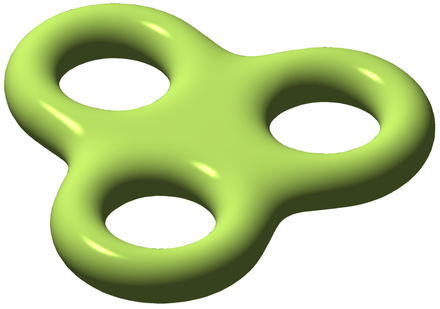
\includegraphics[scale = 1]{RiemannSurface}
**** Riemann Surface of genus 3, from Wikimedia ****

Of course this definition does not apply to curves over fields other than $\CC$, and doesn't relate the genus to the algebra of the curve. However, we can relate the topological genus of a curve directly to its topological Euler characteristic. Since $C$ is topologically compact, connected, and oriented, we have
$H^{0}(C; \ZZ)=H^{2}(C; \ZZ) = \ZZ$, so:
$
\chi_{top}(C) = 2-2g.
$
By the Hopf index theorem, the topological Euler characteristic is the degree of the tangent sheaf, or equivalently, minus the degree of the cotangent sheaf $\omega_{C}$; that is, $\deg K_{C} = 2g-2$, and thus
$$
g(C) = \frac{\deg(K_C)}{2} + 1.
$$
This formula serves to define the genus of a smooth projective curve over any field. 
Other characterizations of the genus require more machinery to establish. We will state some here, and use  tools from the following section to prove equivalence.

\begin{enumerate}

\item 
$
g(C) = 1 - \chi(\cO_C). \label{pa}
$

\item\label{genus Hilbert} If $C \subset \PP^r$ is a smooth curve of degree $d$  with homogeneous coordinate ring
$S_C$, then for sufficiently large $d$ the function $m \mapsto h_C(m) := \dim_\CC (S_C)_m$ is equal to a linear function
$$
p_C(m) =  dm - g + 1,
$$
so $g(C) = dm+1-p_C(m)$. 

\item\label{genus 1forms} $g(C)$ is the dimension of the vector space of regular 1-forms (that is, global sections of the
canonical sheaf) on $C$.
\end{enumerate}

\subsection{Arithmetic genus and geometric genus}
In this section, we'll deal with a  curve $C_0$ that is assumed to be reduced and irreducible.
Any reduced, irreducible 1-dimensional scheme $C_0$ has a normalization $\nu: C \to C_0$ which is a birational
map from a smooth curve. The genus of $C$ is called the \emph{geometric genus} of $C_0$.


The geometry of singular curves is a fascinating topic, from the local analysis of the singularities to the global questions involving linear series on singular curves, and most of the results of this book have analogues for singular curves. But this is a topic beyond the scope of this book; for us, the questions are about smooth curves, with singular curves appearing as a useful adjunct, for example in Chapter~\ref{PlaneCurveChapter}.

Applied to a possibly singular or even non-reduced 1-dimensional projective scheme, the formula~\ref{pa} and the equivalent~\ref{genus Hilbert}, define
what is called the \emph{arithmetic genus} $p_a(C)$. 

We can relate the two notions via the map of sheaves
$$
\cO_{C} \to \nu_*\cO_C.
$$
This is injective; the cokernel sheaf will be a skyscraper sheaf supported exactly on the singular points of $C_0$. Denoting this sheaf by $\cF$, we have an exact sequence
$$
0 \to \cO_{C_0} \to \nu_*\cO_C \to \cF \to 0.
$$

The normalization map $\nu: C \to C_0$ is finite, so that the higher direct images $R^i\nu_*\cO_C = 0$ for $i > 0$; it follows from the Leray spectral sequence that $\chi(\nu_*\cO_C) = \chi(\cO_C)$. Thus
$$
p_a(C_0) - g(C) =  \chi(\cO_{C}) -   \chi(\cO_{C_0}) = \chi(\cF) = h^0(\cF);
$$ 
in other words, the difference between the arithmetic and geometric genera of $C_0$ is the sum of the vector space dimensions of the stalks on $\cF$; colloquially, it's the number of linear conditions a function $f$ on $C$ has to satisfy to be the pullback of a function from $C_0$. The length of the stalk of $\cF$ at a particular singular point $p \in C_0$ is called the \emph{$\delta$-invariant of the singularity}; to rephrase the statement above in these terms, we have
$$
p_a(C_0) - g(C) = \sum_{p \in (C_0)_{sing}} \delta_p
$$ 

The $\delta$ invariant of a singularity is easy to compute in simple cases. For example:
\begin{enumerate}

\item (nodes) If $p \in C_0$ is a node, with points $r,s \in C$ lying over it, the condition for a function $f$ on $C$ to descend is simply that $f(r)=f(s)$; this is one linear condition and accordingly $\delta_p = 1$.

\item (cusps) If $p \in C_0$ is a cusp, with  $r \in C$ lying over it, the condition for a function $f$ on $C$ to descend is simply that the derivative $f'(r)=0$; again, this is one linear condition and accordingly $\delta_p = 1$.

\item (tacnodes) Suppose now that $p \in C_0$ is a \emph{tacnode}, that is, $C_0$ has two smooth branches at $p$ simply tangent to one another. There will be two points $r, s \in C$ lying over it, and the condition for a function $f$ on $C$ to descend is that in terms of suitable local coordinates both $f(r)=f(s)$ and $f'(r)=f'(s)$.  This represents two linear conditions and accordingly $\delta_p = 2$.

\item (planar triple points) Next up, consider an ordinary triple point $p \in C_0$ of a plane curve: that is, a singularity consisting of three smooth branches meeting pairwise transversely, such as the zero locus of $y^3-x^3$. There will be three points $r,s,t \in C$ lying over $p$, and certainly a necessary condition for a function $f$ on $C$ to descend is that $f(r)=f(s)=f(t)$---two linear conditions. But there's a third, less obvious linear condition: in order for $f$ to descend, the derivatives $f'(r), f'(s), f'(t)$ have to satisfy a linear condition---a reflection of the fact that a function on $C_0$ cannot vanish to order 2 on each of two branches without vanishing to order 2 along the third as well. Thus $\delta_p = 3$

\item (spatial triple points) We will be concerned in what follows only with planar singularities, but spatial triple points provide a useful contrast to the last example. A spatial triple point is a singularity consisting of three smooth branches, with linearly independent tangent lines, so that its Zariski tangent space is 3-dimensional. An example would be the union of the three coordinate axes in $\AA^3$.

In this case, in contrast to the last one, the condition that $f(r)=f(s)=f(t)$ is both necessary and sufficient for $f$ to descend, and accordingly we have $\delta_p=2$.

\end{enumerate}

\begin{exercise}
Let $p \in C$ be a singular point of a reduced curve $C$. Show that if $\delta_p = 1$, then $p$ must be either a node or a cusp.
\end{exercise}



\subsection{The Riemann-Roch Theorem}

To prove that these formulas for the genus are correct, we use \trr and Serre duality (sometimes called Kodaira-Serre duality, since Kodaira was responsible for the analytic version.)

\begin{theorem}[Riemann-Roch Theorem]\label{RR}
 If $C$ is a smooth, connected projective curve of genus $g$, and $D$ a divisor of degree $d$ on $C$ then
$$
h^0(D) = d - g + 1 + h^0(K_C - D).
$$
\end{theorem}

For example, if we take $D=0$, this tells us that $h^0(K) = g$, proving the characterization~(\ref{genus 1forms}) above. Using this and \trr for $D=K$
we get $\deg K = 2g-2$. Also, since $h^0(D) = 0$ for any divisor $D$ of negative degree, the formula gives the dimension of $h^{0}(D)$ when $\deg D$ is large:

\begin{corollary}\label{nonspecial RR}
For any divisor $D$ of degree $d$ we have
$$
h^0(D) \geq d - g + 1,
$$
with equality if $d > 2g-2$.
\end{corollary}
This was the theorem originally proven by Riemann; his student Roch supplied the correction term $h^0(K_C - D)$ for divisors of lower degree.
The dimension $h^0(K_C-D) = h^1(D)$ was called the \emph{superabundance} of $D$.

Corollary~\ref{nonspecial RR} and Proposition~\ref{very ample} together show that all high degree divisors come from hyperplane sections in 
suitable embeddings:

\begin{corollary}\label{degree 2g+1 embedding}
Let $D$ be a divisor of degree $d$ on a smooth, connected projective curve of genus $g$. If $d \geq 2g$, the complete linear series $|D|$ is base point free; and if $d \geq 2g+1$ the associated morphism $\phi_D : C \to \PP^{d-g}$ is an embedding, so that
$D$ is the preimage of the intersection of $C$ with a hyperplane in $ \PP^{d-g}$.
\end{corollary}

Since the complement of a hyperplane in projective space is an affine space, we get an affine embedding result too:

\begin{corollary}
 If $C$ is any smooth, connected projective curve and $\emptyset \neq \Gamma \subset C$ a finite subset then $C \setminus \Gamma$ is affine.
\end{corollary}
\begin{proof}
Let $D$ be the divisor defined by $\Gamma$. By Corollary~\ref{degree 2g+1 embedding} a high multiple of $D$ is very ample,
and gives an embedding $\phi: C\to \PP^n$ such that the preimage of the intersection of $C$ with some hyperplane $H$
is a multiple of $D$. It follows that $C\setminus \Gamma$ is embedded in $\AA^n = \PP^n\setminus H$.
\end{proof}
 
We can  use Corollary~\ref{nonspecial RR} to determine the Hilbert polynomial of a projective curve. To do this, let $C \subset \PP^r$ be a smooth curve of degree $d$ and genus $g$, and consider the exact sequence of sheaves
$$
0 \rTo \cI_{C/\PP^r}(m) \rTo \cO_{\PP^r}(m) \rTo \cO_C(m) \rTo 0
$$
and the corresponding exact sequence
$$
 H^0(\cO_{\PP^r}(m)) \rTo^{\rho_m} H^0(\cO_C(m)) \rTo H^1(\cI_{C/\PP^r}(m)) \rTo 0.
$$

The \emph{Hilbert function} $h_C$ of $C$  is defined by
$$
h_C(m) = \dim_{\CC} (S_{C})_{m} = \rank(\rho_m).
$$
By Theorem~\ref{Serre vanishing} we have $H^1(\cI_{C/\PP^r}(m)) = 0$ for large $m$, so $h_{C}(m) = h^0(\cO_C(m))$ for large $m$, which, by the Riemann-Roch theorem, equals $md-g+1$, again for large $m$. Thus, the Hilbert polynomial of $C \subset \PP^r$ is $p_C(m) = dm-g+1$, establishing the characterization~(\ref{genus Hilbert}).
 
The Riemann-Roch formula does \emph{not} give us a formula for the dimension $h^0(D)$ when $h^0(K_C - D)>0$; such divisors $D$ are called \emph{special divisors}, or \emph{special divisor classes}. The existence or non-existence of divisors $D$ with given $h^{0}(D)$ and $h^{1}(D)$ often serves to distinguish one curve from another, and will be an important part of our study.

\begin{fact}
If $k$ is a field that is not algebraically closed there may be smooth projective genus 0 curves over $k$ that are not isomorphic to $\PP^1$. However, they must be ``forms'' of $\PP^1$ in the sense that they become isomorphic to $\PP^1$ after extension of scalars to 
the algebraic closure $\overline k$ of $k$. The unique example with $k = \RR$ is the conic $x^2+y^2+z^2 = 0$. Indeed, any form of $\PP^1$ over any field $k$ can  be embedded in $\PP_{k}^2$  using the anti-canonical linear system.

The curve $\PP_k^1$ itself may be described as the scheme of left ideals of $k$-vector-space dimension 1 in the ring of
$2\times 2$ matrices over $k$ (such an ideal can be embedded in the matrix ring as a linear combination of the 2 columns in an appropriate sense). More generally, any scheme that is a form of $\PP^1$ over $k$
may be described as the scheme of 1-dimensional left ideals in a 4-dimensional central simple ($=$ Azumaya) algebra over $k$. For example, the
conic $x^2+y^2+z^2 = 0$ with no points over $\RR$ is the scheme of left ideals in the algebra of quaternions.\end{fact}

\subsection{A partial proof}

If, following~\ref[Chapter IV]{H} we take the definition of the genus of  a smooth connected curve $C$ to be $h^1(\sO_C)$ (so that $g = h^0(K_C)$ becomes a Corollary of Theorem~\ref{sd}), then it is easy to establish the following form of the Riemann-Roch Theorem:

\begin{corollary}
 If $C$ is a smooth, connected projective curve and $D$ is a divisor on $C$ then
$$
\chi(\sO_C(C)) := h^0(D) - h^1(D) = d-g+1
$$
or in other words, for any invertible sheaf $\cL$ of degree $d$ on $C$,
$$
\chi(\cL) = d-g+1.
$$
\end{corollary}
\begin{proof}
 Taking $D=0$ the statement becomes $h^0(\sO) - h^1(\sO) = 1-g$, which is our definition of $g$. On the other hand,
for any divisor $D$ on $C$ and any point $p \in C$ we have an exact sequence of sheaves
$$
0 \to \cO_C(D-p) \to \cO_C(D) \to \frac{\cO_C(D)}{\gm_{C,p}\cO_C(D)} \to 0
$$
Since $\cO_C(D)$ is locally isomorphic to $\sO_C$ we see that $\cO_C(D)/\gm_{C,p}\cO_C(D)\cong \kappa(p)$ is a sky-scraper sheaf of dimension 1, concentrated at $p$,
and thus has Euler characteristic 1. 
\end{proof}


Thus the Riemann-Roch Theorem for $\cO_C(D)$ is equivalent to the Riemann-Roch Theorem for $\cO_C(D-p)$. Since any divisor can be obtained from 0 by adding and subtracting points, the Riemann-Roch formula for an arbitrary $\cL$ follows from the special case $\cL = \cO_C$.

\subsection{Clifford's theorem}

While the Riemann-Roch Theorem gives a lower bound for the dimension of a linear system, $r(\sL) := h^0(\sL)-1 \geq \deg \sL -g$, Clifford's Theorem
gives an upper bound. If $\deg \sL>2g-2$, then the Riemann-Roch inequality becomes an equality, so it is enough to treat the case $\deg \sL \leq 2g-2$.
To state the sharpest form, we define a curve $C$ of genus $\geq 2$ to be \emph{hyperelliptic} if there exists a $g^1_2$ on $C$; that is an
invertible sheaf $\cL$ of degree $2$ with 2 independent global sections. We will see in Chapter~\ref{genus 2 and 3 chapter} that such a sheaf would be unique, and $h^0(\cL) = 2$.


\begin{theorem}\label{Clifford}
Let $C$ be a curve of genus $g$ and $\cL$ a line bundle of degree $d \leq 2g-2$. Then
$$
r(\cL) \leq \frac{d}{2}.
$$
Moreover, if  equality holds then we must have either
\begin{enumerate}
\item $d=0$ and $\cL = \cO_C$;
\item $d = 2g-2$ and $\cL = K_C$; or
\item $C$ is hyperelliptic, and $|\cL|$ is a multiple of the $g^1_2$ on $C$.
\end{enumerate}
\end{theorem}

\fix{We haven't defined ``hyperelliptic" at this point, or talked about ``the $g^1_2$". Should we just state the weak form of Clifford here, or should we move the definition of hyperelliptic?}

The proof of the inequality will follow easily from a basic result about the addition of linear series, defined as follows:
$\cD = (\cL,V)$ and $\cE = (\cM, W)$ be two linear series on a curve $C$. By the \emph{sum} $\cD + \cE$ of $\cD$ and $\cE$, we will mean the pair 
$$
\cD + \cE = (\cL \otimes \cM, U) 
$$
where $U \subset H^0(\cL \otimes \cM)$ is the subspace generated by the image of $V \otimes W$, under the multiplication/cup product map $H^0(\cL) \otimes H^0(\cM) \to H^0(\cL \otimes \cM)$---in other words, it's the subspace of the complete linear series $|\cL\otimes \cM|$ spanned by divisors of the form $D+E$, with $D \in \cD$ and $E \in \cE$.
 
\begin{proof}
If $\cD$ and $\cE$ are two nonempty linear series on a curve $C$, then
$$
\dim(\cD + \cE) \geq \dim \cD + \dim \cE.
$$
To see this, we observe that to say $\dim \cD \geq m$ means exactly that we can find a divisor $D \in \cD$ containing any given $m$ points of $C$; since $\cD + \cE$ contains all pairwise sums $D + E$ with $D \in \cD$ and $E \in \cE$, we can certainly find a divisor $F \in \cD + \cE$ containing any given $\dim \cD + \dim \cE$ points of $C$.

The proof of the inequality in Clifford's Theorem follows  by applying this observation to the pair $|\cL|$ and $|K_C\otimes \cL^{-1}|$: by 
the Riemann-Roch Theorem, we have
$$
r(K_C\otimes \cL^{-1}) = r(\cL) +g - d - 1
$$
and so we deduce that
$$
g = r(K_C) + 1 \geq r(\cL) + r(K_C\otimes \cL^{-1}) + 1 \geq 2r(\cL) +g - d;
$$
hence $r(\cL) \leq d/2$.

For the proof of the second half of Clifford we will use a basic fact about the geometry of hyperplane sections of a curve in projective space (Proposition~\ref{monodromy of hyperplane section}); we defer it to there.
\end{proof}



\section{The canonical morphism}

Given the central role played by the canonical divisor class, it is natural to look at the geometry of the morphism $\phi_K : C \to \PP^{g-1}$ associated to the complete canonical series $|K|$.  

\begin{definition}
A curve $C$ of genus $g \geq 2$ is said to be \emph{hyperelliptic} if there exists a morphism $f: C \to \PP^1$ of degree 2. \end{definition}

\begin{theorem}\label{canonical system is very ample}
If $C$ is a smooth curve of genus $\geq 2$ then the canonical morphism $\phi_K : C \to \PP^{g-1}$ is an embedding if and only if $C$ is not hyperelliptic.
\end{theorem}

\begin{proof}
By Corollary~\ref{degree 2g+1 embedding} we have to show that for any pair of points $p, q \in C$ we have
$$
h^0(K_C(-p-q)) = h^0(K_C)-2 = g-2.
$$
Applying \trr we see this fails if and only if $h^0(\cO_C(p+q)) \geq 2$ for some $p,q \in C$. By Lemma~\ref{deg 2 morphism}, this implies that $C$ is hyperelliptic.
\end{proof}

\begin{lemma}\label{deg 2 morphism}
Let $C$ be a smooth, projective curve of genus $g\geq 2$. If $C$ has an invertible sheaf $\cL$ of degree 2 with two independent sections, then
$|\cL|$ defines a morphism of degree 2 to $\PP^{1}$, and $C$ is hyperelliptic. In particular, if $g(C) = 2$ then the canonical series $|K_{C}|$ defines a 2 to 1 morphism to $\PP^{1}$, so $C$ is hyperelliptic.
\end{lemma}

\begin{proof}
If $\cO_C(p+q)$ has two independent sections and has $d$ basepoints, then it defines a morphism of degree $2-d$ to $\PP^1$. Since $C$ is not rational,
we must have $d=0$, proving the first statement. 
\end{proof}

\subsection{The geometric Riemann-Roch theorem}

If $C$ is a nonhyperelliptic curve, embedded in $\PP^{g-1}$ by its canonical series and  $D = p_1+\dots + p_d$ is a divisor consisting of $d$ distinct points, let $\overline D$ be the span of the points $p_i \in C \subset \PP^{g-1}$. Since the hyperplanes in $\PP^{g-1}$ containing $\{p_1,\dots,p_d\}$ correspond (up to scalars) to sections of $K_C$ vanishing at all the points $p_i$, we see that
$$
h^0(K_C-D) = g - 1 - \dim \overline D.
$$
Plugging this into the Riemann-Roch formula, we arrive at the statement
$$
r(D) = d - 1 - \dim \overline D;
$$
or in other words, the dimension of the linear series $|D|$ in which the divisor $D$ moves is equal to the number of linear relations on the points $p_i$ on the canonical curve. Thus, for example, if $D = p_1+p_2+p_3$, we see that $D$ moves in a pencil if and only if the points $p_i$ are collinear.

We can extend this statement to the case of arbitrary effective divisors $D$ on any smooth curve if we define our terms correctly. To do this, suppose $f : C \to \PP^d$ is any morphism, and $D \subset C$ any divisor. We define the \emph{span} of  $f(D)$ to be the intersection
$$
\overline{f(D)} = \bigcap_{H \mid f^{-1}(H)\supset D} H 
$$
of all hyperplanes in $\PP^d$ whose preimage in $C$ contains $D$. The argument above applies to prove:

\begin{theorem}[Geometric Riemann-Roch Theorem]\label{geometric RR}
If $C$ is any curve of genus $g \geq 2$,  $\phi : C \to \PP^{g-1}$ its canonical morphism and $D \subset C$ any effective divisor of degree $d$, then
$$
r(D) = d - 1 - \dim \overline{\phi(D)}.
$$
\end{theorem}
 
 \section{Canonical Curves}\label{Noether theorem section}

When we analyze the embedding of a curve $C\subset \PP^n$ we generally ask first whether $C$ is contained in any low-degree
hypersurfaces, and if so how many, in the sense of the dimension $(I_C)_d)$ the degree $d$ part of the homogeneous ideal of $C$.
From the long exact sequence in cohomology
$$
0\to H^0(\sI_{C/\PP^n}(d)) \to H^0(\sO_{\PP^n}(d)) \to H^0(\sO_C(d)) \to H^1(\sI_{C/\PP^n}(d)) \to H^1(\sO_{\PP^n}(d)) \to\cdots
$$
together with the facts that  $H^0(\sO_{\PP^n}(d))$ is the vector space of degree $d$ forms on $\PP^n$ and 
 $H^1(\sO_{\PP^n}(d)) = 0$ for $n>1$ and $d\geq 0$, we see that
 $$
 \dim (I_C)_d = h^0(\sI_{C/\PP^n}(d)) = h^0(\sO_{\PP^n}(d)) - h^0(\sO_C(d)) + h^1(\sI_{C/\PP^n}(d)).
$$
If $d$ times the degree of $C$ is $>2g-2$, the the Riemann-Roch Theorem tell us the value of
 $h^0(\sO_C(d))$, and thus a lower bound for $ \dim (I_C)_d$, but if, in addition, the map
 $H^0(\sO_{\PP^n}(d) \to H^0(\sO_C(d))$ is surjective (or equivalently $h^1(\sI_{C/\PP^n}(d))=0$),
 then we get $ \dim (I_C)_d$ exactly.
 
 
\begin{definition} An embedding of a smooth curve
$C\subset \PP^n$ is said to be \emph{projectively normal} if all the maps $H^0(\sO_{\PP^n}(d)) \to H^0(\sO_C(d))$ are surjective,
or equivalently $h^1(\sI_{C/\PP^n}(d))=0$ for all $d\geq 0$.
\end{definition}
 
By Serre's Criterion of Normality  a 1-dimensional scheme  $C\subset \PP^n$
is a smooth, projectively normal curve iff the homogeneous coordinate ring of $C$ is a normal ring, whence the terminology in
this definition. The criterion has two parts, which are interesting separately: A local or graded ring is normal if it is nonsingular in
codimension 1; and
locally of depth $\geq 2$ in codimension $\geq 2$. In the case of the homogeneous coordinate ring of a curve, 
the first condition means that the curve is nonsingular and the second means that $h^1(\sI_{C/\PP^n}(d))=0$ for all $d$.
In particular, for any very ample invertible sheaf $\sL$ on a smooth curve $C$, the ring 
$$
R(C, \sL) := \bigoplus_{m=0}^\infty H^0(\sL^m)
$$
is normal. See for example \cite[Theorem ***]{Eisenbud1995}.

\begin{example}\label{rnc is projectively normal}
For $d\geq 1$ the rational normal curve $C\subset \PP^d$ of degree $d$ is projectively normal. 
We have $H^0(\sO_{\PP^1}(md))  = \CC[s,t]_{md}$. Th natural natural map
$$
\CC[x_0,\dots,x_d] \to\bigoplus_{m = 0}^\infty H^0(\sO_{\PP^1}(md)));\quad x_0,\dots, x_d \mapsto s^d,s^{d-1}t,\dots, t^d
$$ 
is surjective since every monomial of degree $md$ can be written as a monomial in  
the elements $s^d,s^{d-1}t,\dots, t^d$, and the ring is normal (Exercise~\ref{normality of RNC}).
\end{example}

\begin{exercise}\label{normality of RNC}
 Show that $\CC[s^d,s^{d-1}t,\dots, t^d]$ is normal (ie, integrally closed) by noting that its integral closure must be
 contained in $\CC[s,t]$ and then showing that if $f$ is any polynomial
 in the integral closure then the homogeneous components of $f$ are also in the integral closure.
\end{exercise}


We will now show that the canonical image of a smooth curve is always projectively normal. When the curve is hyperelliptic,
the canonical image is the rational normal curve, treated above, so we may assume that the curve $C$ is embedded
by $|K_C|$ as a smooth curve in $\PP^{g-1}$.


To do this we will make use of an auxiliary construction, a \emph{simple $(g-4)$-secant $(g-3)$-plane.}

\begin{lemma}
 If $C\subset \PP^n$ is a reduced, irreducible, nondegenerate curve, and $m\leq n-1$, then the linear span $L := \overline{p_1,\dots, p_m}$
 of $m$ general points of $C$ is a simple $m$-secant; that is, a plane of dimension $m-1$ such that
 $C\cap L = \{p_1,\dots,p_m\}$ scheme-theoretically.
 \end{lemma}
 
 
\begin{proof}
The plane $L$ is contained in a hyperplane $H$, and since the points are general, we may take this to be a general hyperplane. By Bertini's Theorem, $C\cap H$ is reduced, so $C\cap L$ is also reduced.
 If $C\cap L$ had length $>m$, then by Lemma~\ref{general position lemma} every set of $m+1$ points of $C\cap H$ would be dependent,
 and the span of $C\cap H$ would thus have dimension $\leq m-1<n-1$, and we could choose a hyperplane section $C\cap H'$ with more points than $C\cap H$, which is absurd.
\end{proof}

The following was proven by Max Noether, Emmy's father:

\begin{theorem}[Max Noether]\label{canonical curves are ACM}
A canonical curve in $\PP^{g-1}$ has degree $2g-2$ and arithmetic genus $g$. If the curve has a simple
$g-2$ secant, then it is arithmetically Cohen-Macaulay; that is,
$\HH^{1}(\sI_{C/\PP^{g-1}}(m)) = 0$ for all $m\in \ZZ$.
\end{theorem}
 
For a canonically embedded irreducible curve the simple $g-3$-dimensional $g-2$ secant planes $\Lambda$  correspond to base-point-free pencils of degree $g = 2g-2 -(g-2)$: Given $\Lambda$, the linear series of hyperplanes containing $\Lambda$ intersects $C$ in $\Lambda$ plus the fibers of this pencil. Conversely, given such a pencil, the plane is the span of the complement of a general  member $P$ of the pencil in  $C\cap \overline P$, where $\overline P$ is the hyperplane that is the linear span of $P$.
   
\begin{proof} The Hilbert polynomial $\chi_{C}(t) = h^{0}\sO(t)-h^{1}\sO(t)$ of $C$ has degree equal to
$\dim C = 1$, so it is determined by two values.

We begin by showing that $\sO(-m)$ has no global sections for $m>0$.
If $D$ is a divisor equivalent to $m$ times the hyperplane section, we have an exact sequence
$$
0\to \HH^{0}(\sO_{C}(-m)) \to \HH^{0}(\sO_{C}) \to \HH^{0}(\sO_{D}) \to \cdots.
$$
By hypothesis, the vector space $\HH^{0}\sO_{C}$ is spanned by the constant functions, and these
restrict non-trivially to $\sO_{D}$, and $\HH^{0}(\sO_{C}(-m)) = 0$ as claimed.

Using the Riemann-Roch Theorem we can now compute the Hilbert function $\chi_{C}(m)$:
We have 
\begin{align*}
 \chi_{C}(0) &= h^{0}(\sO_{C}) - h^{1}(\sO_{C}) = h^{0}(\sO_{C}) - h^{0}(\omega_{C}) = 1-g.\\
\chi_{C}(1) &= h^{0}(\sO_{C}(1)) - h^{1}(\sO_{C}(1)^{*}\otimes \omega_{C}) = h^{0}(\omega_{C}) - h^{0}(\sO_{C}) = g-1.
\end{align*}
and we deduce
$\chi_{C}(m) = (2g-2)m -g+1$, whence we see that the degree of $C$ is $2g-2$ and $p(C) = g$ as claimed.

To show that
$C$ is arithmetically Cohen-Macaulay we use the sequence
$$
\cdots \to \HH^{0}(\sO_{\PP^{n}}(m)) \to \HH^{0}(\sO_{C}(m))
\to \HH^{1}(\sI_{C}(m))\to \HH^{1}(\sO_{\PP^{n}}(m)) \to\cdots .
$$
Since $\HH^{1}(\sO_{\PP^{n}}(m)) = 0$, it
is enough to show that the natural map 
$$
\HH^{0}(\sO_{\PP^{n}}(m)) \to \HH^{0}(\sO_{C}(m))
$$
 is surjective for all $m\in \ZZ$. For $m=0,1$ this is immediate from the hypothesis.

For $m <0$ we must show $\HH^{0}(\sO_{C}(m))=0.$ 
If $D$ is a divisor equivalent to $-m$ times the hyperplane section, we have an exact sequence
$$
0\to \HH^{0}(\sO_{C}(m)) 
\to \HH^{0}(\sO_{C}) 
\to \HH^{0}(\sO_{D}) \to \cdots.
$$
By hypothesis, the vector space $\HH^{0}\sO_{C}$ is spanned by the constant functions, and these
restrict non-trivially to $\sO_{D}$, so the kernel, $\HH^{0}(\sO_{C}(m))$, is 0 as claimed. 

To prove surjectivity for $m\geq 2$ we use the remaining hypothesis, the existence of
a simple $g-3$-dimensional $g-2$ secant plane $\Lambda$  and an idea sometimes called the \emph{base-point-free pencil trick}. Let $p_{0},\dots p_{g-3}$ be the points in which $\Lambda$ meets $C$.  Since the
$p_{i}$ are linearly independent by hypothesis, we may choose homogeneous coordinates $x_{i} \in \HH^{0}(\sO_{C}(1))$ so that
$x_{i}(p_{j}) \neq 0$ if and only if $i = j$. It follows that the sections
$x_{i}^{m}$ of $\sO_{C}(m)$ span $\HH^{0}(\sO_{C}(m)|_{\{p_{0}, \dots, p_{g-3}\}})$. Let 
$V\subset \HH^{0}(\sO_{C}(1))$ be the two-dimensional subspace of linear forms vanishing on
$\Lambda$, and thus on the $p_{i}$. 

For $m\geq 2$ there are maps of vector spaces
$$
\wedge^{2} V\otimes \HH^{0}(\sO_{C}(m-2)) \to V\otimes \HH^{0}(\sO_{C}(m-1)) 
\to \HH^{0}(\sO_{C}(m))
$$
where the right hand map is multiplication and the left hand map sends
$s_{1}\wedge s_{2}\otimes \sigma$ to $s_{1}\sigma-s_{2}\sigma$ for any local section $\sigma$.
The sequence is exact because the sections $s_{1},s_{2}$ that span $V$ never vanish simultaneously except on the $p_{i}$, and has image  consisting of sections that vanish on the points $p_{i}$

\end{proof}

\begin{corollary}\label{canonical hilbert function}
If $C\subset \PP^{g-1}$ is a canonical curve with a simple $g-3$-secant, then the Hilbert function of the homogeneous coordinate ring $S_{C}$ of  $C$ depends only on $g$, and is given by:
$$
\dim({S_{C}})_{d} = h^{0}(\cO_{C}(d)) = 
\begin{cases}
 0 &\mbox {if } d<0\\
 1 & \mbox {if }  d=0\\
 g & \mbox {if }  d=1\\
 (2n-1)g+1 & \mbox {if }  d>1\\
\end{cases}
$$
\end{corollary}
\begin{proof}
Theorem~\ref{canonical curves are ACM} implies, in particular, that the homogeneous coordinate ring of $C$ can be identified with 
$\oplus_{n\in \ZZ}\HH^0\sO_C(n)$.  
\end{proof}

 \section{A bit about surfaces}
 We will often analyze curves  on a smooth surface; here are a few results that will be useful. We refer to~\cite[Chapter V]{Hartshorne1977}
 and~\cite[Chapter I]{Beauville} for proofs.
 
 We suppose for this section that $X$ is a smooth projective surface.
 We define $\Pic(X)$ to be the group whose elements are invertible sheaves on $X$.
When two divisors $D,E$ on $X$ meet transversely we define $D\cdot E$ to be the number of points in which they meet. If they have no common
components, we can still define a non-negative intersection multiplicity $m_X(D,E,p)$ at each point $p$, and then set
$$
D\cdot E = \sum_p m_X(D,E,p).
$$
Over the complex numbers each codimension 1 subvariety $D$ of $X$ has a fundamental class
$[D]\in H^2(X, \ZZ)$ and the product is the cup product with values in $H^4(X,\ZZ)$, which is $\ZZ$ since $X$ is compact and orientable. Thus
there is an extension of the product to the cases where $D,E$ have common components. From a geometric point of view, we may choose an
appropriate $C^\infty$
normal vector field along $E$ and define $E'$ by ``pushing'' $E$ out slightly along the direction of this field, until $D$ and $E'$ are transverse,
and the intersections can be computed in the usual way. It should be noted that such intersection numbers can be either positive or negative,
since they depend on the relative orientations of $D$ and $E'$ at the intersection points; this is in contrast to the case when $D$ and $E$
themselves meet properly; in this case the fact that the complex numbers are canonically oriented makes the intersection number non-negative.

The intersection product can also be defined algebraically, over any field: Setting $\sL := \sO_X(C)$ and
$\sM := \sO_X(D)$ to simplify the notation, we set 
$$
D\cdot E = \chi(\sO_X)-\chi(\sL^{-1}) -\chi(\sM^{-1}) -\chi(\sL^{-1}\sM^{-1}) 
$$
\begin{theorem} The pairing $(D,E) \mapsto (D.E)$ is the unique bilinear map
$\Pic(X) \times \Pic(X) \to \ZZ$ extending the case of intersections of two transverse curves on $X$. 
\end{theorem}

A frequent use of the the intersection pairing is to compute the (arithmetic) genus of a curve on a surface,
a result called the adjunction formula.

\begin{theorem}[Adjunction Formula]\label{adjuction formula}
If $C$ is a curve lying on a smooth surface $X$ then 
$$
\omega_C = \omega_X \otimes \sO_X(C) \otimes \sO_C.
$$
In particular \label{genus formula}
$$
p_a(C) = \frac{(K_X+C)\cdot C}{2} +1
 $$
\end{theorem}

We will frequently be interested in curves on quadrics in $\PP^3$, and we can spell out the
intersection theory on these surfaces very concretely; see for example~\cite[****]{Hartshorne1977}.
We will treat them and the curves on them in detail in Section~\ref{curves on scrolls} as part of the larger family of 2-dimensional rational normal scrolls; for
now we sketch the situation as an example of the theory of this section. 

\begin{example}[Quadrics in $\PP^3$]\label{Div of quadric}
 
Quadric surfaces $S$ in $\PP^3$ are classified by their rank:
\begin{itemize}
\item A quadric of rank 2 is the union of two planes; it cannot contain an nondegenerate irreducible curve
\item A rank 3 quadric $S$ is a cone over a plane conic. Suppose that $C$ is a smooth,
curve on such a quadric:
\begin{itemize}
\item  If $C$  does
not pass through the vertex then it is the intersection of the quadric with a hypersurface of some
degree $d$. In this case $C$ has degree $2d$ and genus $(d-1)^2$. 
 \item if $C$ passes through the vertex, then $C$ lies in the divisor class of a line through the origin plus the intersection of $S$ with a hypersurface of some degree $d$. In this case $C$ has degree $2d+1$ and 
 genus $d(d-1)$. 
\end{itemize}

%If  it contains smooth irreducible curves that do not pass through the vertex of the cone, and smooth irreducible curves that of
%degree $2d$ that are intersections of $S$ with hypersurfaces of degree $d$; and smooth 
%irreducible curves of degree $2d+1$ that 

\item A quadric of rank 4 is nonsingular, and is isomorphic to $\PP^1\times \PP^1$.


\item The Picard group of $\PP^1\times \PP^1$ is $\ZZ\oplus \ZZ$, generated by the 
classes of the lines $\{p\}\times \PP^1$ and $\PP^1\times \{p\}$, where $p\in \PP^1$
is any point. These lines have self-intersection 0, and meet transversely in a point,
so the intersection pairing is given by $(a,b)\cdot(c,d) = ad+bc$. From the adjunction formula
applied to the classes of the lines $(1,0)$ and $(0,1)$ we that the canonical
class is $(-2,-2)$, and thus the arithmetic genus of a curve of type $(a,b)$ is thus
$$
\left(((a,b)+(-2,-2))\cdot (a,b)\right)/2 +1 = (a-1)(b-1).
$$

\item Writing $\pi_1, \pi_2$ for the two projections of
$\PP^1\times \PP^1 \to \PP^1$, the sheaf 
$$
\sL := \sO_{\PP^1\times \PP^1}(a,b) = \pi_1^*\op1a \otimes \pi_2^*\op1b
$$
has cohomology given by the K\"unneth formula, for example
\begin{align*}
 H^0(\sL) &= H^0(\op1a)\otimes H^0(\op1b) \hbox{ and thus }\\
 h^0(\sL) &= (a+1)(b+1) \hbox{ if } a\geq 0, b\geq 0.
\end{align*}

\item Any smooth quadric surface $S\subset \PP^3$ is the 
image of $\PP^1\times \PP^1$ embedded by the complete linear system
$|\sO_{\PP^1\times \PP^1}(1,1)|$ and thus contains two families of lines. 
A curve in the class $(a,b)$ thus has degree $(a,b)\cdot(1,1) = a+b$. 
\end{itemize}
\end{example}

Often we wish to compute the dimension of the space of sections of an invertible sheaf, but
as with the case of curves, the Euler characteristic is more accessible:

\begin{theorem}[Riemann-Roch for surfaces] Let $\sL$ be an invertible sheaf on a smooth surface $S$.
the Euler characteristic $\chi(D) := h^0(\sL)-h^1(\sL)+h^2(\sL)$, where $\sL = \sO_S(D)$, is given by
$$
\chi(D) = \chi(\sO) + \frac{(D-K_S)\cdot D}{2}+1
$$
\end{theorem}

\fix{Possible addition:  the Hodge Index theorem as corollary. This could be used to prove finiteness of the automorphism group of a curve following Hartshorne V Ex. 1.11, perhaps in place of the proof now in the inflections chapter.}

It is useful to know what happens under mappings of surfaces, particularly the case of the mapping
corresponding to blowing up a point.

\begin{theorem}
If $\pi: X \to Y$ is a birational map of smooth surfaces, then the pullback map on divisors
preserves the intersection pairing. If $X$ is the blowup of $Y$ at a point $p$, with exceptional
divisor $E = \pi^{-1}(p)$ then:

\begin{enumerate}
 \item $\Pic X =\pi^*(\Pic Y) \oplus \ZZ E$.
\item The canonical class on $X$ is given by $K_X = \pi^*(K_Y)+E$.
 \item The intersection pairing on $\Pic X$ is given by
 
\begin{itemize}
\item $\pi^*(D)\cdot\pi^*(D') = D.D'$ for all $D,D'\in \Pic Y$.
\item $\pi^*(D)\cdot E = 0$ for all $D\in \Pic Y$.
 \item $E\cdot E = -1$.
 \item $K_X\cdot E = -1$.
 \item If $C$ is a curve that has an $m$-fold point at $p$ then $\pi^{-1}(C)$ contains $E$ with multiplicity $m$.
 \end{itemize}
\end{enumerate}
\end{theorem}

Blowups occur frequently in the theory of surfaces, and are easy to characterize:
\begin{theorem}
If $E\subset X$ is a curve on a smooth projective surface $X$ and
 that $E^2 = E\cdot K_X = -1$ then $E$ can be ``blown down'' in the sense that
 $X$ is the blowup of a smooth surface $Y$ at a point $p\in Y$, and $E$ is the exceptional divisor.
\end{theorem}


\input footer.tex
%header and footer for separate chapter files

\ifx\whole\undefined
\documentclass[12pt, leqno]{book}
\usepackage{graphicx}
\input style-for-curves.sty
\usepackage{hyperref}
\usepackage{showkeys} %This shows the labels.
%\usepackage{SLAG,msribib,local}
%\usepackage{amsmath,amscd,amsthm,amssymb,amsxtra,latexsym,epsfig,epic,graphics}
%\usepackage[matrix,arrow,curve]{xy}
%\usepackage{graphicx}
%\usepackage{diagrams}
%
%%\usepackage{amsrefs}
%%%%%%%%%%%%%%%%%%%%%%%%%%%%%%%%%%%%%%%%%%
%%\textwidth16cm
%%\textheight20cm
%%\topmargin-2cm
%\oddsidemargin.8cm
%\evensidemargin1cm
%
%%%%%%Definitions
%\input preamble.tex
%\input style-for-curves.sty
%\def\TU{{\bf U}}
%\def\AA{{\mathbb A}}
%\def\BB{{\mathbb B}}
%\def\CC{{\mathbb C}}
%\def\QQ{{\mathbb Q}}
%\def\RR{{\mathbb R}}
%\def\facet{{\bf facet}}
%\def\image{{\rm image}}
%\def\cE{{\cal E}}
%\def\cF{{\cal F}}
%\def\cG{{\cal G}}
%\def\cH{{\cal H}}
%\def\cHom{{{\cal H}om}}
%\def\h{{\rm h}}
% \def\bs{{Boij-S\"oderberg{} }}
%
%\makeatletter
%\def\Ddots{\mathinner{\mkern1mu\raise\p@
%\vbox{\kern7\p@\hbox{.}}\mkern2mu
%\raise4\p@\hbox{.}\mkern2mu\raise7\p@\hbox{.}\mkern1mu}}
%\makeatother

%%
%\pagestyle{myheadings}

%\input style-for-curves.tex
%\documentclass{cambridge7A}
%\usepackage{hatcher_revised} 
%\usepackage{3264}
   
\errorcontextlines=1000
%\usepackage{makeidx}
\let\see\relax
\usepackage{makeidx}
\makeindex
% \index{word} in the doc; \index{variety!algebraic} gives variety, algebraic
% PUT a % after each \index{***}

\overfullrule=5pt
\catcode`\@\active
\def@{\mskip1.5mu} %produce a small space in math with an @

\title{Personalities of Curves}
\author{\copyright David Eisenbud and Joe Harris}
%%\includeonly{%
%0-intro,01-ChowRingDogma,02-FirstExamples,03-Grassmannians,04-GeneralGrassmannians
%,05-VectorBundlesAndChernClasses,06-LinesOnHypersurfaces,07-SingularElementsOfLinearSeries,
%08-ParameterSpaces,
%bib
%}

\date{\today}
%%\date{}
%\title{Curves}
%%{\normalsize ***Preliminary Version***}} 
%\author{David Eisenbud and Joe Harris }
%
%\begin{document}

\begin{document}
\maketitle

\pagenumbering{roman}
\setcounter{page}{5}
%\begin{5}
%\end{5}
\pagenumbering{arabic}
\tableofcontents
\fi


\chapter{The Riemann--Roch theorem}\label{RiemannRochChapter}

\section{How many sections?}

To study curves via their maps to projective spaces, we want to estimate the dimension of the space of global
sections of an invertible sheaf $\cL$. The beginning
of the story is the Riemann--Roch theorem.

Though we would like to be able to compute $h^0(\sL)$, it is much
easier to compute the 
\blue{Euler characteristic}
\index{Euler characteristic}%
$$
\chi(\sL):= \sum_{i\geq 0} (-1)^i h^i(\sL).
$$
This computes $h^0(\cL)$ itself in many cases, by virtue of the following result:
\marginpar{indexed theorem name}

\begin{theorem}[Serre--Grothendieck vanishing theorem]
\label{Serre--Grothendieck vanishing}
\index{Serre--Grothendieck vanishing theorem}%
\index{vanishing theorem!Serre--Grothendieck}%
If $\sF$ is a coherent sheaf on a projective scheme $X$ of dimension $n$, then for any $i$, the vector space $H^i(\sF)$ is finite-dimensional, and is 0 if  $i> n$. Moreover,
if $X\subset \PP^m$ then for $d\gg 0$, $\sF(d)$ is generated by its global sections and $H^i(\sF(d)) = 0$ for all $i>0$.\qed
\end{theorem}

\begin{proof}
This is a combination of 
theorems due to Grothendieck and Serre. See
\cite[Theorems III.2.7 and III.5.2]{Hartshorne1977}, 
and
also \cite{Serre1955} for a 
reasonably
concrete proof.
\end{proof}

A 
shortcoming
of this vanishing theorem is the lack of a bound on the number $d$ needed to achieve the second assertion. For smooth curves
and invertible sheaves
this is corrected by Theorem~\ref{RR theorem}, which gives a bound in terms of the genus and the degree.

One immediate consequence of Theorem~\ref{Serre--Grothendieck vanishing} is that on a smooth variety the groups of invertible sheaves and divisor classes are the same:

\begin{corollary}\label{invertible sheaves and divisors}
If $X$ is a projective variety that is nonsingular in codimension $1$,
every invertible sheaf $\cL$ on $X$ is of the form $\cL =\cO_C(D)$ for some 
\index{Cartier divisor}\index{divisor!Cartier}%
Cartier divisor $D$ on $X$. Thus if $X$ is a smooth projective variety
\index{notation!div}%
the map $\div$ is an isomorphism from the group of invertible sheaves
to the group 
of divisor classes.
\end{corollary}

\begin{proof}
Let $H \subset \PP^r$ be a general hyperplane, and $E$  the divisor  of intersection of $C$ with $H$. We know that for $n \gg 0$, $\cL(n)$ has sections; and if $F$ is the divisor of zeroes of one such section, we have
$$
\cL = \cO_C(F - nE).
$$
If $X$ is smooth, then, since a regular local ring is a unique
factorization domain, every codimension-one subvariety is defined locally 
by a single nonzerodivisor, and thus corresponds to a Cartier divisor.
This implies that $\div$ is surjective. Furthermore any 
\blue{isomorphism between invertible sheaves}
\index{invertible sheaf!isomorphism between -s}%
is defined by multiplication with a global rational function, so that invertible sheaves defining linearly equivalent divisors are
isomorphic. Thus $\div$ is injective as well.
\marginpar{(de): this proof is pretty swift, and the result fundamental. Let's give a Hartshorne citation too.}
\end{proof}

\subsection*{Riemann--Roch without duality}

It follows from Theorem~\ref{Serre--Grothendieck vanishing} that on
any scheme $X\subset \PP^r$ we have $\chi(\sL(d)) = h^0(\sL(d))$ for
large $d$, 
and that $\chi(\sL) = h^0(\sL) - h^1(\sL)$ in the case of a curve.

\begin{theorem}[easy Riemann--Roch]\label{easy RR}
If $C$ is a smooth projective curve, and $\sL$ is an invertible sheaf on $C$, then $\chi(\sL) = \deg \sL + \chi(\sO_C)$.
\index{Riemann--Roch theorem!easy}%
\end{theorem}

\begin{proof}
 The result is tautological if $\sL = \sO_C$. Every invertible sheaf on $C$ has the form $\sL = \sO_C(D)$ for some
divisor $D$. If $p\in C$, then writing $\kappa(p)$ for the
structure sheaf of the subscheme $p\in C$, the long exact sequence in cohomology
associated to the short exact sequence
$$
0\to \sL(-p) \to \sL \to \sL\otimes \kappa(p)\to 0
$$
together with the isomorphism $\sL\otimes \kappa(p) \cong \kappa(p)$
and the vanishing of higher cohomology of a sheaf with zero-dimensional support allows us to compute 
$$
\chi(\sL) = \chi(\sL(-p)) + \chi(\kappa(p)) = \chi(\sL(-p)) + 1.
$$
Since every divisor on $C$ can be reached by adding and subtracting points, this suffices.
\end{proof}

Since the Euler characteristic of a sheaf is well-behaved, we can extend the result of Theorem~\ref{easy RR} 
to invertible sheaves on any one-dimensional scheme $C$, by defining
$\deg \sL := \chi(\sL) -\chi(\sO_C)$.
We will use this definition to express the self-intersection of a divisor on a surface in Section~\ref{surface basics}.

We can make the Riemann--Roch theorem still more useful by understanding the error term $h^1(\sL)$. This requires
the canonical divisor and Serre duality, to which
we now turn.


\section{The most interesting linear series}\label{most interesting}

The most important vector bundles on a manifold are the tangent and cotangent bundles. For reasons that
will become clear, the focus in algebraic geometry is on the cotangent
bundle or, equivalently, the sheaf of differential 1-forms. On a
smooth curve $C$ the \emph{canonical sheaf} is the sheaf of
differentials, which is an 
\index{canonical sheaf}\index{sheaf!canonical}\index{sheaf!of differentials}%
invertible sheaf; on a smooth
variety of dimension $n$ we define the canonical sheaf to be the 
$n$-th exterior power of the sheaf of differentials. A section of 
$\omega_C$ is thus a differential form, and the class of the divisor
of such a form is usually denoted 
\blue{$K_C$.}
\index{notation!$K_C$}%

\begin{fact}
Canonical sheaves are defined for any projective scheme; see 
Definition~\ref{dualizing sheaf for singular curve}.
They are usually called 
\index{dualizing sheaf}\index{sheaf!dualizing}%
{\it dualizing sheaves} 
in that generality. The condition for the dualizing sheaf to be an invertible
\index{Gorenstein scheme}%
sheaf is that the scheme is (locally) Gorenstein, something that is true, for example, for any subscheme of $\PP^r$
that is locally a complete intersection (see Section~\ref{dualizing sheaves section}).
\end{fact}
 

On projective space we can compute the canonical sheaf directly; other computations of the canonical sheaf will usually reduce to this central case.

\begin{theorem}
 The 
\blue{canonical sheaf of $\PP^{r}$}
\index{canonical sheaf!of $\PP^{r}$}%
is $\sO_{\PP^{r}}(-r-1)$. 
\vspace*{-\parskip}
\end{theorem}

\begin{proof}
Let $x_{0}, \dots, x_{r}$ be the projective coordinates on $\PP^{r}$
and let  $U = \PP^{r}\setminus H$ be the affine open set where $x_{0}
\neq 0$. Thus $U \cong \AA^{r}$ with coordinates $z_{1} :=
x_{1}/x_{0}$, $\dots$, $z_{r}:=x_{r}/x_{0}$. The space of
$r$-dimensional differential forms on $U$ is spanned by
$d(x_{1}/x_{0})\wedge\cdots\wedge d(x_{r}/x_{0})$, which is regular
everywhere in $U$. In view of the formula
$$
d\frac{x_{i}}{x_{0}} = \frac{x_{0}\,dx_{i}-x_{i}\,dx_{0}}{x_{0}^{2}}
$$
we get
$$
d\frac{x_1}{x_0}\wedge\cdots\wedge 
d\frac{x_r}{x_0}
= \frac{dx_{1}\wedge\cdots\wedge dx_{r}}{x_{0}^{r}}-
\sum_{i=1}^{r} x_{i} \frac{ dx_{1}\wedge\cdots \wedge \widehat{dx_{i}}\wedge \cdots \wedge dx_{r}}{x_{0}^{r+1}}
$$
which has a pole of order $r+1$ along the locus $H$ defined by $x_{0}$. Thus the divisor of this differential form
is $-(r+1)H$, and this is the canonical class.
\end{proof}

\begin{fact}
A different derivation: there is a short exact sequence of sheaves,
\index{Euler sequence}%
\marginpar{Ch. II $\to$ II (or else Chapter II, \S8 if you feel it's safer)}
called the Euler sequence \cite[II.8]{Hartshorne1977}:
$$
0\to \Omega_{\PP^{r}} \to \sO_{\PP^{r}}^{r+1} (-1) \to \sO_{\PP^{r}} \to 0.
$$
Summing over all twists, and taking global sections, that is, applying $H^0_*$, we see that 
$H^0_*(\Omega_{\PP^{r}})$ fits into an exact sequence:
$$
0 \to H^0_*(\Omega_{\PP^{r}}) \to S^{r+1}(-1) \ruto{\delta_{1}} S \to \CC \to 0,
$$
where $S$ is the homogeneous coordinate ring of $\PP^r$ and $\delta_1$ sends the $i$-th basis vector of
$S^{r+1}(-1)$ to the $i$-th variable of $S$; that is, $H^0_*(\Omega_{\PP^{r}})$ is the second syzygy of the residue field $\CC$ of $S$. We can extend this sequence to the Koszul complex that is the free resolution
of $\CC$, 
\index{Koszul complex}%
\cite[\S17.5]{Eisenbud1995}:
$$
0 \to S(-r-1) \ruuto{\delta_{r+`1}} 
\mwedge^rS^{r+1}(-r) \ruto{\delta_{r}} \cdots \to S^{r+1}(-1) \to S \to \CC \to 0.
$$
For each $i$, the $i$-th exterior power of the map $H^0_*(\Omega_{\PP^{r}}) \to S^{r+1}(-1)$ is an inclusion, and
represents $\mwedge^i(\Omega_{\PP^{r}})$ as the sheaf associated to the graded module that is the $(i+1)$-st syzygy of $\CC$.
In particular, the canonical module $\omega^{}_{\PP^r} = \mwedge^r(\Omega_{\PP^{r}})$ is the sheaf associated to the 
$(r+1)$-st syzygy, $S(-r-1)$.

For more on syzygies, see Chapter~\ref{SyzygiesChapter}.
\end{fact}

The most important invariant of a smooth curve can be defined in terms of the canonical sheaf:

\begin{definition}
If $C$ is an irreducible smooth curve we define the genus $g(C)$ to be the dimension of $H^0(\omega_C)$.
\end{definition}

Computations of the canonical sheaf on a variety usually involve
comparing the variety to a variety 
whose
canonical sheaf is already known. The most useful results of this type
are  the \emph{adjunction formula}
and \emph{Hurwitz's theorem}. 

\subsection*{The adjunction formula}%\label{Adjunction Formula}

In the simplest case, the adjunction formula says that the canonical divisors of a smooth plane 
curve $C$ of degree $d$ are the intersections of $C$ with curves of degree $d-3$ 
(see Figure~\ref{canonical of quartic}). 
More generally, for a divisor $X$ on a smooth variety $Y$, it says that
the canonical sheaf on $X$ is $\omega_Y(X)|_X$. This is an immediate consequence of
the still more general formula below because the normal bundle of $X$ is $\sO_Y(X)$.

In general, the adjunction formula describes the difference between the canonical divisor of
a  subscheme and the restriction of the canonical divisor from the ambient variety.
If $X\subset Y$ we define the \emph{conormal sheaf} of $X$ in $Y$ to be $\sI_{X/Y}/\sI_{X/Y}^{2}$,
and the \emph{normal sheaf} of $X$ in $Y$ to be its dual, 
$$
\sN_{X/Y} = \sHom(\sI_{X/Y}/\sI_{X/Y}^{2}, \sO_{Y}).
$$
If $X$ and $Y$ are smooth, $X$ is locally a complete intersection in $Y$, so
 $@\sI_{X/Y}/\sI_{X/Y}^{2}$ 
is a vector bundle on $X$ of rank equal to the codimension, $\dim Y -\dim X$.
 When, in addition, the codimension is 1, so that $X$ is a divisor and $\sI_{X} = \sO_{Y}(-X)$, we get
 $$
 \sN_{X/Y} = \sO_{X}(X).
 $$


\begin{proposition}[adjunction formula]\label{adjunction}
 Let $X\subset Y$ a smooth subscheme of codimension $c$ in a smooth variety $Y$, and let $K_{Y}$ be the canonical class of $Y$. The canonical class $K_X$ of $X$ is 
\index{adjunction formula}\index{formula!adjunction}%
 $$
 \omega_{X} = \mwedge^{c} \sN_{X/Y} \otimes \omega_{Y}.
 $$
In particular, when $X$ is a divisor, $K_{X}$ is the restriction to $X$ of the divisor $K_{Y}+X$ on $Y$.
\end{proposition}

\begin{figure}
\centerline{\includegraphics[width=2.5in]{"main/Fig02-1"}}
\caption{On a smooth plane quartic, the canonical divisors are its
  intersections with lines.
}\label{canonical of quartic}
\end{figure}


\begin{proof}
 Because $X$ is locally a complete intersection in $Y$ there is an exact sequence of sheaves
 $$
0\to  \sI_{X/Y}/\sI_{X/Y}^{2} \to \Omega_{Y}| _{X} \to \Omega_{X} \to 0
,
 $$
 where $\Omega_{X}$ is the sheaf of differential forms on $X$ (see \cite[Proposition 16.3]{Eisenbud95}), and
$ \sI_{X/Y}|_{X} = \sO_{Y}(-X)|_{X} = \sO_{X}(-X)$. The proposition follows by taking top exterior powers, 
as in Lemma~\ref{exterior powers}.\end{proof}

\begin{lemma}\label{exterior powers}
 If 
$$
0\to \sE \to \sF\to \sG \to 0
$$
is a short exact sequence of locally free sheaves of ranks $e,f,g$ 
 on a scheme $X$, then there is a natural
isomorphism 
$$
\mwedge^e\sE \otimes \mwedge^g \sG \to \mwedge^f\sF.
$$
\end{lemma}

\begin{proof}[Proof of Lemma~\ref{exterior powers}]
 We may define a map
$
\mwedge^e\sE \otimes \mwedge^g \sG \to \mwedge^f\sF
$
in terms of local sections as
$$
(\epsilon_1\wedge\cdots \wedge \epsilon_e) \otimes (\gamma_1\wedge\cdots\wedge \gamma_g)
\mapsto \epsilon_1\wedge\cdots \wedge \epsilon_e\wedge\gamma_1\wedge\cdots\wedge \gamma_g.
$$
This is globally well-defined because changing one of the $\gamma_i$ by a local section of $\sE$ would not
change the exterior product.
To check that the map is an isomorphism, it is enough to show that this is true locally.

Because $\sG$ is locally free, there is a covering of $X$ by open sets $U$
so that the sequence
$$
0\to \sE|_U \to \sF|_U\to \sG|_U \to 0
$$
is a split exact sequence of free modules, $\sF|_U = \sE|_U\oplus \sG|_U$.
It follows that
$$
\mwedge^f\sF|_U = 
\tsty\bigoplus\limits_{i+j = f} \mwedge^i \sE|_U \otimes \mwedge^j\sG|_U.
$$
In our case all the exterior powers of $\sE$ vanish above the $e$-th, and all the 
exterior powers of $\sG$ vanish above the $g$-th, so 
$$
\mwedge^f\sF|_U =  \mwedge^e \sE|_U \otimes \mwedge^g\sG|_U,
$$
with isomorphism given as above.
\end{proof}


\begin{corollary}\label{canonical of plane curve}\label{canonical of complete intersection}
If $C\subset \PP^{2}$ is a smooth plane curve of degree $d$, then
$\omega_{C} = \sO_{C}(d-\nobreak 3)$; more generally, if
$X\subset \PP^{r}$ is a smooth complete intersection of hypersurfaces of degrees $d_{1},\dots, d_{c}$ in $\PP^r$ then
$\omega_{X} = \sO_{X}(\sum d_{i }-r-1).$
\vspace*{-3pt}
\end{corollary}

\begin{proof}
Since $\sN_{X/Y} = \bigoplus\limits_{i=1}^{c} \sO_{X}(d_{i})$, the result follows from Theorem~\ref{adjunction}.
\end{proof}

\subsection*{Hurwitz's theorem}
 Given a (nonconstant) morphism $f : C \to X$ of smooth projective
 curves, the Riemann--Hurwitz formula computes the canonical sheaf
 $C$ in terms of that of  $X$ and the local geometry of $f$. To do
 this we define the
\index{Hurwitz's theorem}\index{theorem!of Hurwitz}%
\index{Riemann--Hurwitz formula}\index{formula!Riemann--Hurwitz}%
\index{ramification index}%
\blue{\emph{ramification index}}%
of $f$ at $p \in C$,  denoted $\ram(f,p)$, 
by the formula 
$$
 f^{-1}(q) = \!\sum_{\substack{\,p\in C\\ f(p)=q}}\! (\ram(f,p)+1)\cdot p
 $$
 for any point $q \in X$. 

\begin{proposition}
If $f : C \to X$ is a (nonconstant) morphism  of smooth projective curves,
there are only finitely many
points $p\in C$ such that $\ram(f,p)>0$.
\end{proposition}

In light of this result we define the \emph{ramification divisor}
\index{ramification divisor}% 
of $f$ to be the divisor
 $$
 R = \sum_{p \in C} \ram(f,p)\cdot p \; \in \;  \Div(C).
 $$
 and the \emph{branch divisor} to be
 $$
 B = \sum_{q \in X} \Big(\sum_{p \in f^{-1}(q)} \ram(f,p) \Big)\cdot q \; \in \; \Div(X).
 $$
Note that $R$ and $B$ have the same degree, which is $\sum_{p \in C} \ram(f,p)$.

\begin{proof}
The result follows from the separability of the map of fields of rational functions, $K(X) \to K(C)$, which holds because we
are in characteristic 0 (in characteristic $p$ the 
\blue{Frobenius map}
\index{Frobenius map}%
provides a counterexample). A proof using separability
is given in~\cite[Section IV.2]{Hartshorne1977}. Here is an analytic version:

In terms of local parameters $z$ on $C$ around $p$ and $w$ on $X$ around $f(p)$, we can write the morphism as $z \mapsto w = z^m$ for some integer $m > 0$; that is,
if $w$ is a local parameter on $X$ and $z$ is a local parameter in the source, then
the map
$$
 \CC\{` `\{w\}` `\} \cong \widehat\sO_{X,f(p)} \ruto{\hat f^*}\widehat\sO_{C,p}\cong  \CC\{` `\{z\}` `\} 
$$ 
of convergent power series rings induced by $f^*$
sends $w$ to $uz^m` `$, where $u$ is a power series with nonvanishing constant term.
In this case $\ram(f,p) = m-1$. These power series expansions are valid in a neighborhood
of $p$, and the derivative of $f$ vanishes at the ramification points in this neighborhood. Since
the zeros of a nonconstant analytic function are isolated, the ramification points are isolated. 
Since $C$ is compact in the classical topology, there are only finitely many.
\end{proof}

Hurwitz's theorem describes the difference between the canonical
divisor of $C$ and the pullback of the canonical divisor of $X$.
\index{Hurwitz's theorem}%

\begin{theorem}[Hurwitz's theorem] 
{\rm\cite[Proposition IV.2.3]{Hartshorne1977}} \label{Hurwitz}
If $f:C\to X$ is a nonconstant morphism of smooth curves, with ramification divisor $R$, then 
$$
K_C = f^{*}(K_{X})+R,$$
or equivalently
$
\omega_{C} = (f^{*}\omega_{X})(R).
$
\end{theorem}
 
\begin{proof}
Let $B$ be the branch divisor of $f$.
Choose a rational 1-form $\omega$ on $X$, and let $\eta = f^*(\omega)$
be its pullback to $C$. 
Since we have the freedom to multiply by any rational function on $X$,
we can arrange for 
the zeroes and poles of $\omega$ to 
avoid
$B$, so that $\omega$ 
is
regular and nonzero at each branch point. (Actually the calculation
goes through even without this assumption, albeit with more
complicated notation.)  

With this arrangement,
for every zero of $\omega$ of multiplicity $m$ we have exactly $d$
zeroes of $\eta$, each with multiplicity $m$; and likewise for the
poles of $\omega$. 
 At a point $p$ where (locally) $f$ has the form $z \mapsto w = z^{e}$
and $\omega = dw$, we have $\eta = z^{e-1}@dz$; that is, $\eta$ has a zero of multiplicity $\ram(f,p)$ at  $p$.
Thus the divisor $K_{C}$ of $\eta$ is
$K_{C} = f^{*}(K_{X})+R$.
\end{proof}

\begin{example}
Let $C\subset \PP^2$ be a smooth plane curve and let $p$ be a point of $\PP^2$ not on $C$. Suppose that the coordinates on $\PP^2$ are chosen so that the ideal sheaf of $p$ is  
 generated by the vector space of linear forms $W = \langle x_0,x_1\rangle$. 
The linear series $(\sO_C(1), W)$ defines the projection of $C$ from $p$ to $\PP^1` `$, a map of degree
$d = \deg C$ (see Figure~\ref{projection of cubic}).

\begin{figure}   % appears as 2.2
\centerline {\includegraphics[height=1.8in]{"main/Fig02-ProjectionPlaneCubic"}}
\captionPlus{Fig02-ProjectionPlaneCubic}{Projection of a plane cubic from a general point $p$ to $\PP^1$ is a three-to-one map.
}
\label{projection of cubic}
\end{figure}

The canonical sheaf of $\PP^1$ has degree $-2$, so by Hurwitz's theorem
$K_C$ has degree $ -2d+ \deg R$, where $R$ is the 
ramification divisor. 
We may choose coordinates
so that none of the branch points lie on the line $x_0 = 0$. Taking this to be the line at infinity, we
may compute 
$R$
after passing to the affine open set $x_0\neq 0$, where the projection
map is given by the function $z = x_1/x_0$.  Suppose that $C$ is defined, in this open set,
by the equation $f(x,y)= 0$. A point $q\in C$ is a 
\index{ramification point}%
ramification
point if the tangent line to $C$ at $q$
passes through $p$, that is, if $dx$  and 
$$
df = \frac{\partial f}{\partial x} dx + \frac{\partial f}{\partial y} dy
$$
\medmuskip1mu
are linearly dependent.
Since $C$ is smooth, $\frac{\partial f}{\partial x} $ and $\frac{\partial f}{\partial y}$ cannot vanish
simultaneously,  this happens if and only if $\partial f/{\partial y}$ vanishes at $q$. The intersection of 
$C$ with the curve defined by $\partial f/{\partial y}=0$ has degree $d(d-1)$ by B\'ezout's theorem,
so the degree of the ramification divisor $R$ is $d(d-1)$. Thus the degree of the canonical
divisor on $C$ is $\deg K_C = -2d@+@d(d-1) = d(d-3)$, which is in accord with 
Corollary~\ref{canonical of plane curve}.
\end{example}

\begin{example}
Let 
$V= H^0(\cO_{\PP^1}(d))$
be the vector space of  homogeneous polynomials of degree $d$ in
two variables. In the
projectivization $\PP(V^{*}) \cong \PP^d` `$, let~$\Delta$ be the
locus of polynomials with a repeated factor. Since $\Delta$ is
defined by the vanishing of the discriminant, it is a hypersurface.
What is its degree? 
 
To answer this, we intersect $\Delta$ with a general line; the degree
of $\Delta$ is the degree of the intersection.  Let $W\subset V$ be a
general 2-dimensional linear subspace, that is, a general pencil of
forms of degree $d$ on $\PP^1` `$. The linear series $\sW =
(\sO_{\PP^{1}}, W)$ defines a morphism $\phi_{\sW} : \PP^{1} \to
\PP(W) \cong \PP^{1}$ and the fiber over the point of $\PP(W)$
corresponding to a form $f$ of degree $d$ is the divisor $\{f =
0\}\subset \PP^{1}$. Thus the intersection of $\Delta$ with the line
is the locus of polynomials in $W$ with a multiple root; that is, the
branch locus of $\phi_{\sW}$, where we would count an $m$-fold root
$m-1$ times if there were multiple roots. 
 By Hurwitz's formula, the degree of the branch locus $B$ of a 
degree $d$ morphism from $\PP^{1}$ to $\PP^{1}$ is
 $$
 \deg B = \deg \omega^{}_{\PP^{1}} - d\deg \omega^{}_{\PP^{1}} = 2d-2.
 $$
 Thus $\deg \Delta = 2d-2$.
 \end{example}
  

\section{Riemann--Roch with duality}

We now return to the task of understanding $h^0(\sL)$ for an invertible sheaf $\sL$ on a smooth curve. Since $\chi(\sL) = h^0(\sL)-h^1(\sL)$ is easier to compute, we would like to understand $h^1(\sL)$ in a more concrete way. The key is duality:
 
\begin{theorem}[Serre duality]\label{sd}
If $C$ is a smooth curve and $D$ is a divisor on $C$, then
\marginpar{indexed ``Serre duality''}%
\index{Serre duality}%
\index{duality!Serre}%
$$
H^1(D) =H^0(K_C-D)^* := \Hom_\CC(H^0(K_C-D), \CC),
$$
and thus $h^1(D) = h^0(K_C-D)$.
\end{theorem}

For proofs see \cite[Theorem III.5.2 and III.7.6]{Hartshorne1977}. 

For example we see that if $C$ is a smooth connected curve then $h^1 (\sO_C) = h^0(K_C) = g(C)$ and thus $\chi(\sO_C) = 1-g(C).$   
Using this we can recast Theorem~\ref{easy RR}
in the more useful form:

\begin{theorem}[Riemann--Roch]\label{RR theorem}
If $D$ is any divisor on $C$, then 
$$
h^0(D) - h^0(K_C -D) = \deg D - g(C) +1.
$$
In particular $\deg K_C = 2g(C) -2$.
\end{theorem}

\begin{proof}
Combine Theorem~\ref{easy RR} with Theorem~\ref{sd}. For the second statement,
apply the formula with $D = K_C$.
\end{proof}

See Sections~\ref{duality} and Theorem~\ref{general RR with duality} for the corresponding results on singular curves.

We can now explain the relationship between the genus of a smooth curve, as we have defined it and the 
topological genus, the ``number of holes'' in the Riemann surface (Figure~\ref{RiemannSurface}):


\begin{figure}   % appears as 2.3
\vskip-20pt
\rotatebox{15}{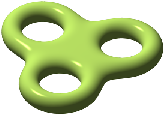
\includegraphics[scale=1.25]{main/Fig02-RiemannSurface}}
\vskip-15pt
\caption{A Riemann surface of genus 3.
\marginparhere{\redden{call in text?}}
}
\label{RiemannSurface}
\end{figure}


\begin{fact} (Hodge theory)
The sole topological invariant of a smooth projective curve $C$,
viewed as an analytic space, is its genus. As a manifold it is a
compact, oriented surface, and its genus is half the rank of its first
singular cohomology, $H^{1}(C; \CC)$, which is equal to its first 
de Rham 
cohomology.
Breaking up the de Rham cohomology of any smooth projective complex variety $X$ in terms of holomorphic and antiholomorphic differential
forms we get the \emph{Hodge decomposition}
$$
H^i(X,\CC) = H^i_{\mathrm{de\,Rham}}(X) = 
\tsty\bigoplus\limits_{j=0}^i H^j(\mwedge^{i-j} \Omega_X).
$$
For a smooth curve $C$, this says in  particular that
$$
H^1(C; \CC) = H^0(\omega_C)\oplus H^1(\sO_C) = H^0(\omega_C)\oplus (H^0(\omega_C))^\vee, 
$$
so $ h^0(\omega_C)$ is half the rank of the middle singular cohomology
group, justifying the name ``genus''. For details, 
see~\cite[p.\,116]{Griffiths-Harris1978}.
\end{fact}

A divisor $E$
of negative degree 
satisfies the equation
$H^0(E) = 0$,
so we get the form of the Riemann--Roch theorem
originally proved by 
\blue{Riemann:}
\index{Riemann, Georg}%

\begin{corollary}\label{nonspecial RR}
For any divisor $D$ of degree $d$ we have
$$
h^0(D) \geq d - g + 1,
$$
with equality if $d > 2g-2$.
\end{corollary}
%
It was 
\blue{Gustav Roch,}
\index{Roch!Gustav}%
a student of
Riemann's, 
who supplied the correction term $h^0(K_C - D)$ for divisors of lower degree.
The dimension $h^0(K_C-D) = h^1(D)$ was called the 
\blue{\emph{superabundance}}
\index{superabundance}%
of $D$: the ``expected'' number of sections was $d-g+1$, and $h^1(\cL)$ reflected how much larger the actual number was.

Corollary~\ref{nonspecial RR} and Proposition~\ref{very ample} together show that all high degree divisors come from hyperplane sections in 
suitable embeddings; and unlike the general vanishing theorems, they give a bound on the degree necessary for vanishing
of cohomology and for
global generation:

\begin{corollary}\label{degree 2g+1 embedding}
Let $D$ be a divisor of degree $d$ on a smooth, connected projective curve of genus $g$.
\begin{enumerate}
 \item If $d>2g-2$ then $H^1(\sO_C(D)) = 0$.
 \item If $d \geq 2g$ then $\sO_C(D)$ is generated by global sections; that is, the complete linear series $|D|$ is basepoint free; and $\sO_C(D)$ is very ample unless $D = K_{C}+E$ for some divisor $E$ of degree 2.
 \item If $d \geq 2g+1$ then $\sO_C(D)$ is very ample; that is, the associated morphism $\phi_D : C \to \PP^{d-g}$ is an embedding, and
$D$ is the preimage of the intersection of $C$ with a hyperplane in $ \PP^{d-g}$.
\end{enumerate}
\end{corollary}

\begin{proof}
If $d>2g-2$ then $K-D$ has negative degree, and thus 
$$h^1(D) = h^0(K-D) = 0. $$ 
The last two parts follow
from the Riemann--Roch theorem and Proposition~\ref{very ample}.
\end{proof}

Since the complement of a hyperplane in projective space is an affine space, we get an affine embedding result too:

\begin{corollary}
 If $C$ is any smooth projective curve and $\Gamma \subset C$ a nonempty finite subset then $C \setminus \Gamma$ is affine (that
 is, isomorphic to a closed subscheme of an affine space).
\marginpar{moved period past parens}     
\end{corollary}

\begin{proof}
Let $D$ be the divisor defined by $\Gamma$. By Corollary~\ref{degree 2g+1 embedding} a high multiple of $D$ is very ample,
and gives an embedding $\phi: C\to \PP^n$ such that the preimage of the intersection of $C$ with some hyperplane $H$
is a multiple of $D$. It follows that $C\setminus \Gamma$ is embedded in $\AA^n = \PP^n\setminus H$.
\end{proof}
 
We can  use Corollary~\ref{nonspecial RR} to determine the Hilbert polynomial of a projective curve. To do this, let $C \subset \PP^r$ be a smooth curve of degree $d$ and genus $g$, and consider the exact sequence of sheaves
$$
0 \to \cI_{C/\PP^r}(m) \to \cO_{\PP^r}(m) \to \cO_C(m) \to 0
$$
and the corresponding exact sequence
$$
 H^0(\cO_{\PP^r}(m)) \ruto{\rho_m} H^0(\cO_C(m)) \to H^1(\cI_{C/\PP^r}(m)) \to 0.
$$

The  $h_C$ of $C$  is defined in terms of the
\blue{\emph{Hilbert function}}
\index{Hilbert function}%
homogeneous coordinate ring $R_{C}$ of $C$ by
\marginpar{removed colon}
$$
h_C(m) = \dim_{\CC} (R_{C})_{m} = \rank \rho_m,
\marginparhere{removed parentheses around argument of rank}
$$
where $(R_{C})_{m}$ is the degree $m$ component of the homogeneous coordinate ring of $C$ in $\PP^n` `$.

By Theorem~\ref{Serre--Grothendieck vanishing} we have
$H^1(\cI_{C/\PP^r}(m)) = 0$ for large $m$.
\redden{Therefore}
\marginpar{to allow line break}
$h_{C}(m) = h^0(\cO_C(m))$ for large $m$, which, by 
\redden{Riemann--Roch}, equals $dm-g+1$, again for large $m$. 
Thus, the Hilbert polynomial of $C \subset \PP^r$ is $p_C(m) = dm-g+1$.  
More generally, we define what is called the \emph{arithmetic genus}:

\begin{definition}\label{genus Hilbert}\label{pa}\label{genus formula}
If $C\subset \PP^n$ is a 1-dimensional projective scheme with Hilbert polynomial
$p_C(m) = \chi(\sO_C(m))$, the \emph{arithmetic genus} of $p_a(C)$ is $1-\chi(\sO_{C}) = 1-p_C(0)$. If $C$ is reduced and irreducible, then
the \emph{geometric genus} $g(C)$ is the genus of the normalization of $C$.
\end{definition}

We see from the Riemann--Roch theorem that if $C$ is smooth and connected, then $p_a(C) = g(C) = h^0(\omega_C)$, the genus of $C$. We
will see that for reduced and irreducible curves $p_a(C) \geq g(C)$, with equality only when $C$ is smooth.
  For some examples with curves that are not
reduced and irreducible, see Exercise~\ref{pa example}.
  

The Riemann--Roch theorem and Serre duality have extensions to arbitrary coherent sheaves in place of invertible sheaves 
and to singular curves, which we will explain in Chapter~\ref{LinkageChapter}.

Divisors $D$ for which $h^0(K_C - D)>0$ are called \emph{special divisors}. The existence or nonexistence of divisors $D$ with given $h^{0}(D)$ and $h^{1}(D)$ often serves to distinguish one curve from another, and will be an important part of our study.

\subsection*{Residues, and a complex analytic argument for 
the Riemann--Roch theorem} 

The 
\marginpar{\vskip-35pt \hskip-14pt{\Large$\downarrow$} the hyphen in ``theorem'' is ugly, but I've been unable to fix it. Perhaps drop ``the'' and ``theorem'' around RR? It will lighten up the section title.\\[4pt]dropped ``as well'' after red text.}
Rie\-mann--Roch theorem is so central to the study of curves that it is worth understanding from another point
\redden{of view.}
We remarked at the beginning of Chapter~\ref{linear series} that a
smooth projective curve over $\CC$ is the same thing as a compact
Riemann surface. 
\redden{Here we will briefly adopt}
the complex analytic viewpoint, and give an explanation of 
\index{complex analytic viewpoint}%
\marginpar{\hskip-50pt $\leftarrow$ streamlined; also removed hyphen in ``complex analytic'' in
  section header to agree with this instance and Chapter 1}
a special case of Theorem~\ref{RR theorem}.

If $D = \sum a_ip_i$ is an effective divisor 
\marginpar{new paragraph}
on a compact Riemann surface $X$ then we write $L(D)$ 
for the vector space of meromorphic functions on $X$ with poles of order 
\marginpar{$\leq\,\to$ at most}
at most $a_i$ at $p_i$. 

\begin{theorem}
Let $X$ be a compact Riemann surface of genus $g$, and let $D$ be an effective divisor of degree $d$ on $X$. Suppose that $K-D$ is also effective for some canonical divisor $K$.
The dimension of  $L(D)$ is
$d-g+1+\dim_\CC L(K-D)$.
\end{theorem}
% avoid double skip
Because  meromorphic functions on a Riemann surface are rational functions on the corresponding
algebraic curve, and $L(D) = H^0(\sO_C(D))$, the assertion is equivalent to Theorem~\ref{RR theorem}.

\begin{proof}
% We will prove this using residues, under the additional assumption that  $D$ and $K-D$ are both effective (that is, $D$ is both effective and \emph{special} in the sense that there are nonzero functions
%both in $L(D)$ and in $L(K-D)$.)
%
Recall that the 
\blue{\emph{residue}} 
of a meromorphic 1-form $\phi$ at a
\index{residue}%
point $p$ on $X$ is defined by an integral: choose a disc $\Delta \subset X$ containing $p$ and in which $\phi$ is holomorphic except
\marginpar{replaced \{\string\rm\ res\} by \string\Res\ (defined with \string\operatorname\string) for the reasons explained in my email to the AMS}
for its pole at $p$. The residue $\Res_p(\phi)$ is $\sfrac{1}{2\pi i}$
times the integral of $\phi$ along the boundary of $\Delta$. If $z$ is
a local coordinate on $\Delta$ zero at $p$ and we write the
differential $\phi$ as
{\meshing
$$
\phi = \sum_{i=-n}^\infty \!a_iz^i \,dz
$$
then by Cauchy's formula, the residue of $\phi$ at $p$ is the coefficient $a_{-1}$. 
}

\begin{proposition}\label{residue sum}
 If $\phi$ is a meromorphic differential on a compact Riemann surface $X$, then the sum of the residues of $\phi$
 at all the poles of $\phi$ is $0$.
\marginpar{made 0 upright, ok?}
 \end{proposition}
 
\begin{proof}
Apply 
\blue{Stokes' theorem}
\index{Stokes' theorem}%
to the complement of the union of small discs around each of the poles of $\phi$.
\end{proof}

Let  $D = \sum a_ip_i$ be an effective divisor on $X$, and set $d = \sum a_i = \deg D$. Locally, a function with a pole of order at most $n$ at $p$ may be written in terms of a local coordinate $z$ at $p$ as $\sum_{i=-n}^\infty a_{i}z^{i} $;
the sum $\sum_{i=-n}^{-1} a_{i}z^{i}$ is called its \emph{polar part}.
By the maximum principle, a meromorphic function in $L(D)$ is determined, up to the addition of a constant, by its polar parts at the points~$p_i$. Thus we have $\dim L(D) \leq d+1$.
{\meshing\par}

When is a given collection $c_1,\dots,c_d \in \CC[z^{-1}]$ the polar parts of a global meromorphic function $f$ on $X$? A necessary condition
is that if $\phi \in L(K)$ is a holomorphic differential on $X$, then
$$
\sum \Res_{p_i}(f \cdot \phi) = 0.
$$
This gives $g$ linear relations on the $c_i$. However, if $\phi$ is a holomorphic differential vanishing at all the points $p_i$
then the corresponding relation is trivial. Thus the number of linearly independent relations on the polar parts of $f$ is actually $g - \dim L(K-D)$; and we arrive at an inequality
$$
\dim L(D) \leq d + 1 - g + \dim L(K-D).
$$

This is a priori only an inequality. But we can apply the same logic to an effective divisor $K-D$, and we see that
\begin{align*}
\dim L(K-D) &\leq \deg(K-D) + 1 - g + L(K - (K-D)) \\
& = 2g - 2 - d + 1 - g  + L(D) \\
&= g - d - 1 + L(D).
\end{align*}
Adding the two inequalities we have
\marginpar{\vskip-20pt added period}
$$
L(D) + L(K-D) \leq L(D) + L(K-D).
$$
Since the sum of the inequalities is an equality, we conclude that each inequality is also an equality; this is the Riemann--Roch formula
in our special case.
\end{proof}

\subsection*{Arithmetic genus and geometric genus}

Throughout this book, we will be primarily concerned with the geometry of smooth curves. Of course singular curves will arise\emdash for example, as images of smooth curves under morphisms that are not embeddings. At least when $C$ is a 1-dimensional variety (that is, a 
reduced irreducible 1-dimensional scheme) we can  regard $C$ as the image of a smooth curve in an optimal way:
\marginpar{replaced ``(Proposition~\ref{resolution of singularities})'' by colon}

\begin{proposition}\label{resolution of singularities}
If $C_0$ is a projective variety of dimension 1 then the \emph{normalization} $\phi: C \to C_0$ of $C_0$ is a birational
morphism from a smooth curve $C$. The curve $C$ is again projective, and the pair $(C, \phi)$ is
unique up to  isomorphism. In particular, every birational map of smooth curves is an isomorphism.
\end{proposition}
 
\begin{proof}
  We use the result that the normalization ($=$ integral closure) of a domain
finitely generated over a field is again finitely generated, and nonsingular in codimension 1 \cite[Theorem 4.14 and 11.5]{Eisenbud1995}. Thus,
starting with a projective embedding of $C$ we normalize the homogeneous coordinate ring of $C$. The resulting ring
may have generators in many degrees, but a suitable Veronese subring will be generated in a single degree, and thus
is the homogeneous coordinate ring of a smooth projective curve. 

Localization
\marginpar{reworded to avoid unpleasant hyphens}
commutes with normalization, and any map from a normal ring to a
domain factors uniquely through the normalization. 
\redden{Therefore}
the normalization is unique.
\end{proof}

A different, less canonical procedure for finding a smooth curve birational to a given curve
is explained in 
\marginpar{the xref here was undefined; I assume the last 3 exercises are relevant and coded accordingly. Please check}
\redden{Exercises \ref{Veronese of plane curve} to \ref{Mumford resolution argument}}.


Still assuming that $C_0$ is reduced and irreducible, we can relate
\marginpar{it's it obvious what these terms mean?}
\index{arithmetic genus}%
\index{geometric genus}%
\index{genus!arithmetic versus geometric}%
the
\redden{arithmetic and geometric genera}
of $C_0$ using the map of sheaves
$$
\cO_{C_0} \to \nu_*\cO_C.
$$
Since the normalization map of rings  is injective and finite, this map is injective. The cokernel $\sF$ is a coherent sheaf supported on the singular points of $C_0$, and is thus finite over $\CC$. 
The definition implies that there is a short exact sequence
$$
0 \to \cO_{C_0} \to \nu_*\cO_C \to \cF \to 0.
$$

\begin{proposition}\label{pa and delta}
Suppose that $C_{0}$ is a reduced, irreducible curve and let  $\nu: C\to C_{0}$ be its normalization.
Let $\sF = \nu_{*}\sO_{C}/\sO_{C_{0}}$. If we set 
$\delta(C_{0}) := h^{0}(\sF)$, 
\redden{then}
 $$
p_a(C_0) - g(C) =  \delta(C_{0})
$$ 
\end{proposition}

\begin{proof}
 Since the normalization map $\nu: C \to C_0$ is finite,  the direct images $R^i\nu_*\cO_C$ vanish for $i > 0$, 
so the Leray spectral sequence 
\redden{(see \ref{Leray} just below)}
computes $\chi(\nu_*\cO_C) = \chi(\cO_C)$. Thus
$$
p_a(C_0) - g(C) =  \chi(\cO_{C}) -   \chi(\cO_{C_0}) = \chi(\cF) = h^0(\cF) 
$$ 
since the support of $\cF$ is finite.
\end{proof}

The operation of normalization localizes, so we can understand $\sF$ by looking at it locally.
Writing $R$ for the affine ring of some affine subset $U\subset C_{0}$ we see that $\sO_{C}|_{U}$
is the integral closure $\ovR$ of $R$, so $\sF|_{U}$ is $\ovR/R$. Thus
the annihilator of $\sF|_{U}$, called the \emph{conductor}
$\ff_{\ovR/R}$,
\marginpar{added comma before red phrase}
\redden{is an ideal of both $\ovR$ and $R$,}
and correspondingly $\nu^{-1}(\ff_{C/C_{0}})$ 
is also an ideal sheaf in $\sO_{C}$.

Informally, we may say that $\delta(C_{0})$ is the number of linear
conditions a locally defined function $f$ on $C$ has to satisfy to be
the pullback of a function from $C_0$. The length of the stalk of
$\cF$ at a particular singular point $p \in C_0$ is called the
\index{delta invariant|$\delta$-invariant}
\emph{$\delta$-invariant} $\delta_p$ of the singularity. Thus 
\marginpar{semicolon $\to$ colon; added punctuation in display}
$$
p_a(C_0) - g(C) = \sum_{p @\in@ (C_0)_{\mathrm{sing}}\!\!} \delta_p.
$$ 

\begin{fact}~\label{Leray}
 In general, the 
\blue{Leray spectral sequence}
\index{Leray spectral sequence}%
addresses the situation of  a morphism $f:X\to Y$ of varieties or schemes, 
 and a coherent sheaf $\sG$  on the source $X$; it says in this circumstance that there is a spectral sequence
  $$
  \HH^p(R^qf_*(\sG)) \Longrightarrow \HH^{p+q}(\sG).
  $$
(This is a special case of the spectral sequence for the derived functors of a composite functor ($H^0$ composed with $f_*$);
see~\cite[II.4.17.1]{Godement} or \cite[Section III.7]{Gelfand-Manin} for proofs.)
\end{fact}

In the simplest cases the $\delta$ invariant is easy to compute:


\begin{enumerate}

\item A 
\index{node}%
\blue{\emph{node}}
of a curve $C_0$ is a point $p$ such that
\marginpar{removed ``(nodes)''}
  an analytic neighborhood of $p$ in $C_0$ consists of two smooth arcs
  intersecting transversely at $p$ 
\redden{(See Figure \ref{simplesing}, left.)}
Equivalently, the completion of
  the local ring $\cO_{C_0,p}$ is isomorphic to $k\[x,y\]/(xy)$. If $p
  \in C_0$ is a node, its preimage in the normalization $C$ of $C_0$
  consists of two points $r,s\in C$. The condition for a function $f$
  on $C$ to descend to $C_0$\emdash that is, to be the pullback of a function
on $C_0$\emdash is  that $f(r)=f(s)$; this is one 
linear condition, so $\delta_p = 1$.

\item  
\redden{A}
\index{cusp!ordinary}%
\blue{\emph{cusp}} 
\marginpar{I'm reacting here to the ``(cusps)'' in parens in the versus the term actually defined.}
\redden{(strictly speaking, an \emph{ordinary cusp})}
of a curve $C_0$ is a point $p$
  such that an analytic neighborhood of $p$ in $C_0$ is given by the
  equation $y^2=x^3` `$. 
\redden{(See Figure \ref{simplesing}, second from left.)}
If $p \in C_0$ is an ordinary cusp then its
  preimage in the normalization $C$ of $C_0$ will consist of one point
  $r\in C$. The condition for a function $f$ on $C$  is that the
  derivative $f'(r)=0$; again, this is one linear condition, so
  $\delta_p = 1$. 
\marginpar{moved \string\end\{enumerate\} so the break appears before ``We will''}
\end{enumerate}

We will give more examples at the end of
Chapter~\ref{PlaneCurvesChapter}.



\begin{figure}   % appears as 2.4
\centerline{%
  \includegraphics[height=2in]{"main/Fig02-sing-node"}\hfil\quad
  \includegraphics[height=2in]{"main/Fig02-sing-cusp"}\hfil\quad
  \includegraphics[height=2in]{"main/Fig02-sing-tacnode"}\hfil\quad
  \includegraphics[height=2in]{"main/Fig02-sing-triple"}}
\caption{Simple planar curve singularities.
\index{tacnode}%
\index{triple point}%
\index{planar curve singularities}%
\index{singularity!of planar curve}%
\label{simplesing}
}
\end{figure}


\section{The canonical morphism}

We now return to the world of smooth curves.
\index{canonical morphism}\index{morphism!canonical}%

 The canonical sheaf on $\PP^1$ has negative degree, so $|K_{\PP^1}| = \emptyset$. If $C$ is a curve
 of genus $1$ then the canonical sheaf     has a nonzero global section, and since the sheaf has degree $2g-2=0$ this is nowhere vanishing, whence
 $\omega_C = \sO_C$, and $K_C = 0$. Thus in studying the canonical series we restrict our attention to curves $C$ of genus $g\geq 2$. 
 
 \begin{theorem}\label{canonical series is very ample} Let $C$ be a smooth curve of genus $\geq 2$.
\begin{enumerate}
 \item $|K_C|$ is basepoint free.
 \item $|K_C|$ is very ample if and only if $C$ admits no map of degree 2 to $\PP^1` `$.
\end{enumerate}
\end{theorem}

A curve of genus $\geq 2$
is said to be \emph{hyperelliptic} if there exists a 
\blue{morphism}
$f: C \to \PP^1$ 
\begingroup\def\marginpar#1{}%
\blue{of degree 2.}
\endgroup
\index{hyperelliptic}%
\index{morphism!of degree 2}%
It is easy to describe this in terms of linear series:

\begin{lemma}\label{deg 2 morphism}
Let $C$ be a smooth, projective curve of genus $g\geq 2$. If $C$ has an invertible sheaf $\cL$ of degree $\leq 2$ with two independent sections, then $\cL$ has degree~$2$ and
$|\cL|$ defines a morphism of degree $2$ to $\PP^{1}$, so $C$ is
hyperelliptic. In particular, if $g(C) = 2$ then the canonical series
\marginpar{hyphenated 2-to-1 (and uprighted digits in statements) to agree with the math occurrences}
$|K_{C}|$ defines a $2$-to-$1$ morphism to $\PP^{1}$, so $C$ is
hyperelliptic.
\end{lemma}

\begin{proof}
Since $C \not\cong \PP^1` `$,  Theorem~\ref{characterization of P1} shows that $C$ cannot have a 1-dimensional linear series
of degree $< 2$. Thus $\sL$ has degree exactly 2, and no 
\marginpar{\redden{You defined ``base point'' in chapter 1; this must be the same thing, but here you're writing it as one word. Either is fine, but we should be consistent.  I lean toward no space, since ``base point free'', ``base-point free'' or ``base-point-free'' are all awkward. But it's up to you.}}
\redden{basepoints,}
so it defines a morphism of degree 2 to $\PP^1$ as claimed.
\end{proof}

\begin{proof}[Proof of Theorem~\ref{canonical series is very ample}]
A point $p$ is a basepoint of $|K_C|$ if and only if 
\marginpar{displayed to allow line break}/that
$$h^0(K_C-p) = h^0(K_C) = g.$$ 
By the Riemann--Roch theorem,
this is eqivalent to $h^0(p) =2$, which would imply that $C\cong \PP^1$ by Theorem~\ref{characterization of P1}. Thus $K_C$
has no basepoints.

By Proposition~\ref{very ample} we 
\redden{must}
show that for any 
\redden{two}
points $p, q \in C$ we have
\unskip\marginpar{for better layout}
$$
h^0(K_C(-p-q)) = h^0(K_C)-2 = g-2.
$$
Applying the Riemann--Roch theorem we see 
\marginpar{added ``that'' to allow line break}
that this fails if and only if $h^0(\cO_C(p+q)) \geq 2$ for some $p,q
\in C$. By Lemma~\ref{deg 2 morphism}, this implies that $C$ is
hyperelliptic. Conversely, if $C$ is hyperelliptic then for some
divisor $D = p+q$ we have $h^0(D) = 2$, whence $h^0(K-p-q) = h^0(K)
-1$ by 
the Riemann--Roch formula.
\emergencystretch5.5pt
\end{proof}

The image of the canonical morphism of a nonhyperelliptic curve of
genus $g>2$ is called a 
\blue{\emph{canonical curve},}
\index{canonical curve}%
and (for a nonhyperelliptic curve) we  
speak of the image as being \emph{canonically embedded}.


\subsection*{Geometric Riemann--Roch}

There is a useful way of expressing the Riemann--Roch formula in terms
of the geometry of the canonical map. Suppose $C \subset \PP^r$ is a
smooth curve and $D$ an effective divisor on $C$, thought of as a
subscheme of $C$. We define the 
\blue{\emph{span}}
\index{span!of effective divisor}%
$\ovD$ of $D$ to be the
\marginpar{the index entry is ``span of effective divisor; this covers $\overline{\phi(D)}$ as well, right?}
intersection of the hyperplanes $H \subset \PP^r$ containing $D$. More
generally, if $\phi : C \to \PP^r$ is a map and $D$ an effective
divisor on $C$, we define the span $\overline{\phi(D)} \subset \PP^r$
to be the intersection 
$$
\overline{\phi(D)} := \bigcap_{ 
\substack{H \subset \PP^r \text{ a hyperplane} \\D \subset
  \phi^{-1}(H)}}
H.
\marginparhere{stacked conditions to avoid superwide subscript, ok?}
$$

Now suppose $C$ is a smooth curve of genus $g\geq 2$ and $\phi_K: C\to \PP^{g-1}$ is the canonical morphism.
If  $D$ is an effective divisor on $C$ of degree $d$, then since the hyperplanes in $\PP^{g-1}$ containing $\phi_K(D)$ correspond (up to scalars) to sections of $K_C$ vanishing on $D$, we see that
$$
h^0(K_C-D) = \codim \overline{ \phi_K(D)} \subset \PP^{g-1}= g - 1 - \dim \overline{ \phi_K(D)}.
$$
\index{geometric!Riemann--Roch theorem}%
\index{Riemann--Roch theorem!geometric}%
Applying the Riemann--Roch theorem we obtain  the \emph{geometric Riemann--Roch theorem}:

\begin{corollary}\label{geometric RR}
If $D$ is a divisor on a smooth curve $C$ of genus $\geq 2$ then
$$
r(D) = d - 1 - \dim \overline{ \phi_K(D)}.
\vspace*{-3pt}
$$
\end{corollary}
%
In particular, if $D = \sum_{i=1}^dp_i$ is a sum of distinct points, then
 the dimension of the linear series $|D|$  is equal to the number of linear relations among the images of the $p_i$ on the canonical 
 image of $C$. 
 Thus, for example, a divisor given as the sum $D = p+q+r$ of three
 points will move in a pencil if and only if the three points are
\marginpar{\hskip-100pt $\leftarrow$ colinear $\to$ collinear (there were about equal numbers of each, I uniformized toward the old-fashioned spelling, ok?\\[3pt] streamlined passage in red; original had $\mathrm{p}_{\mathrm{a}})$, but that  seems to have been a coding error}
 collinear on the canonical model. 

In general, 
the condition on forms of degree $d$ to vanish at 
\redden{a given point $p$ in $\PP^r$ is expressed}
by one homogeneous linear
 linear equation on the coefficients of the form, obtained by evaluating the variables at 
 the coordinates of $p$, so vanishing on a set $\Gamma$ of $\gamma$ points is given by
 $\gamma$ linear equations and the same is true when $\Gamma$ is a finite subscheme
 of length $\gamma$, as one sees from the exact sequence
 $$
 0\to H^0(\sI_\Gamma(d) \to H^0(\sO_{\PP^r}(d)) \ruto{ev} H^0(\sO_{\Gamma}(d)) \to 0,
 $$
 bearing in mind that 
 $$
 H^0(\sO_{\Gamma}(d)) \cong H^0(\sO_{\Gamma}) \cong \CC^\gamma.
 $$
However, the linear equations may be linearly dependent; that is, the map marked $ev$
above may have rank $<\gamma$. We will say that the points of $\Gamma$
\emph{fail to impose independent conditions on hypersurfaces of degree $d$}
by the amount equal to $\gamma - \rank(ev)$. 

With this terminology, the geometric Riemann--Roch theorem says that 
the dimension of the complete linear series $|D|$ on a smooth curve $C$
is the amount by which the points of $D$ fail to impose independent conditions
on canonical divisors, and the geometric version simply translates this into 
 hyperplanes in the canonical embedding of $C$. 
\index{Cayley--Bacharach--Macaulay theorem}%
The Cayley--Bacharach--Macaulay
theorem~\ref{CBM} and the result of 
\marginpar{\redden{missing xref `pluricanonical'}}
Exercise~\ref{pluricanonical} are other useful
special cases.

\begin{remark}
For a singular curve $C_0$ to have a canonical morphism it is necessary first of all that its canonical sheaf
 $\omega_{C_0}$ be invertible; when this is the case, we say that $C_0$ is (locally) Gorenstein, and then
\index{locally Gorenstein}%
\index{Gorenstein!locally}%
the theory above can be applied. See for example \cite{graphcurves} and \cite{ribbons} for examples. 
\end{remark}

\subsection*{Linear series on a hyperelliptic curve}
We can describe the canonical map of a hyperelliptic curve\emdash and indeed all its special linear series\emdash quite precisely:

\begin{corollary}\label{canonical on hyperelliptic}
Let $C$ be a smooth hyperelliptic curve of genus $g\geq 2$. The curve $C$ admits a unique degree 2 morphism $\pi: C\to \PP^1` `$,
and the canonical map $\phi_K: C\to \PP^{g-1}$ is the composition of $\pi$ with the Veronese map of degree $g-1$ from
\index{Veronese map}%
$\PP^1$ to the rational normal curve of degree $g-1$; in particular, every canonical divisor is a sum of $g-1$ fibers of $\pi$ and vice versa.
\end{corollary}

\begin{proof}
If $D$ is a general fiber of a degree 2 map $\pi:C\to \PP^1$ so that $D= p+q$ and $r(D) = 1$, then by the Riemann--Roch theorem or its geometric version, $D$ imposes only one condition on sections of $K_C$; that is, $\phi_K(p) = \phi_K(q)$. Consequently the degree of the canonical morphism $\phi_K$ is at least 2, and the image is thus a nondegenerate curve in $\PP^{g-1}$ of degree $\leq (2g-2)/2 = g-1$. By Theorem~\ref{characterization of P1}, the image of $\phi_K$ is the rational normal curve of degree $g-1$ and every fiber of $\phi_K$ is a divisor linearly equivalent to $D$. It follows that $\pi$ is determined by $K$, so it is unique. Since every canonical divisor is the pullback of a hyperplane section of the rational normal curve,
every canonical divisor is a sum of $g-1$ fibers of $\pi$.
\end{proof}

We can use these ideas to analyze all special divisors.
\index{special divisor}%
\index{divisor!special}%

\begin{corollary}\label{special on hyperelliptic} Let $C$ be a smooth 
\blue{hyperelliptic curve}
\index{hyperelliptic curve}%
with map $\pi: C\to \PP^1$ of degree 2.
Every special divisor $D$ of degree $d$ on 
\marginpar{a hyperelliptic curve $\to C$}
$C$ is a sum of $s$ fibers of $\pi$ and $d-2s$ points
$p_1,\dots,p_{d-2s}$ with distinct images under the canonical map; and
in this case we have $r(D) = s$ and the points $p_i$ are base points
of the linear series $|D|$.
\end{corollary}

\redden{Thus}
\emph{no divisor on a hyperelliptic curve is both special and very ample}.
\marginpar{streamlined}

\begin{proof}
Suppose that $D$ contains the sum $E$ of $s$ fibers of $\pi$ and no more; and write $D = E+D'$, with $\deg D' = d-2s$.
 
If $\phi_K:C \to \PP^{g-1}$ is the canonical map, then $\phi_K(D')$ consists of $d-2s$ distinct points, while $\phi_K(E)$ consists of
$s$ points. By Corollary~\ref{independence of points on a RNC} the span of $\phi_K(D)$ has dimension $\min\{g-1, d-s-1\}$, so 
$r(D) = d-1-\min\{g-1, d-s-1\} = \max \{s,d-g\}$. Since $D$ is a special divisor, $r(D) > d-g$, so $r(D) = s$. 
Since $r(E) =s$, we see that $E$ is basepoint free, so $D'$ is the base locus of $D$.
\end{proof}

\section{Clifford's theorem}\label{Clifford Section}

While the Riemann--Roch theorem gives a lower bound for the dimension of a linear series, $r(\sL) := h^0(\sL)-1 \geq \deg \sL -g$, Clifford's theorem
\index{Clifford's theorem}%
gives an upper bound. If $\deg \sL>2g-2$, then the Riemann--Roch
inequality becomes an equality, so it is enough to treat the case
$\deg \sL \leq 2g-2$. The bound is actually a corollary of the 
Riemann--Roch theorem.

\begin{corollary}\label{Clifford bound}
 Let $C$ be a curve of genus $g$ and $\cL$ a line bundle of degree $d \leq 2g-2$. Then
$$
r(\cL) \leq \frac{d}{2}.
$$
\end{corollary}

\begin{proof}
If $\cL$ is nonspecial then, since $g\geq d/2 + 1$, we have $r(\cL) = d-g+1\leq d/2$.
Otherwise we have
$$
r(K_C\otimes \cL^{-1}) = r(\cL) +g - d - 1
$$
by the Riemann--Roch theorem,
and so by Proposition~\ref{sum of linear series}
$$
g = r(K_C)+1  \geq r(\cL) + r(K_C\otimes \cL^{-1}) +1  = 2r(\cL) +g - d;
$$
hence $r(\cL) \leq d/2$.
\end{proof}

The usual statement of Clifford's theorem includes a description of when equality can occur:

\begin{theorem}\label{Clifford}\label{Clifford equality}
Let $C$ be a curve of genus $g$ and $\cL$ a line bundle of degree $d \leq 2g-2$. If
$$
r(\cL) = \frac{d}{2},
$$
the largest possible value, then either
\begin{enumerate}
\item $d=0$ and $\cL = \cO_C@$;
\item $d = 2g-2$ and $\cL = K_C@$; or
\item $C$ is hyperelliptic, and $|\cL|$ is a multiple of the $g^1_2$ on $C$.
\end{enumerate}
\end{theorem}

From Corollary~\ref{canonical on hyperelliptic} and Corollary~\ref{geometric RR} we see that the equality does indeed hold
in each of the cases enumerated. See
Corollary~\ref{equality in Clifford from Martens} for the converse and \cite[IV.5.4]{Hartshorne1977}
for a different proof.

 \section{Curves on surfaces}\label{surface basics}
 
 We will often analyze curves  on a smooth surface. Compared to the theory of linear series on curves, there is a new element: the intersection pairing. We refer to~\cite[Chapter V]{Hartshorne1977}
\index{intersection pairing}%
 and~\cite[Chapter I]{Beauville} for 
\marginpar{``proof'' ok? Or would ``proofs'' be better?}
\redden{proof} 
of the unproven statements in this section.
 We suppose for this section that $S$ is a smooth projective surface,
 and write $\Pic(S)$ for the group of invertible sheaves on $S$.

\subsection*{The intersection pairing}

When two codimension-1 subschemes $D,E$ on $S$ 
\marginpar{upgraded to a subsection (instead of subsub; see also note at top of page 50}
meet transversely we define $D\cdot E$ to be the number of points in which they meet.  
It is less obvious how one might define an intersection number $D\cdot E$ in more general cases,
including the case $D=E$. However 
a codimension-1 subvariety of $S$ has a 
\index{fundamental class}%
fundamental class in $H^{2}(X,\ZZ)$, and the product just defined
agrees with the cup product pairing
\index{cup product pairing}%
$$
H^{2}(S,\ZZ) \times H^{2}(S,\ZZ) \to H^4(S,\ZZ)\cong \ZZ,
$$
showing that it is possible. For example, the self-intersection $D\cdot D$ can be realized geometrically
 by choosing a  vector field $\sigma$ on $D$ and using it to push a copy $D'$ of $D$ infinitesimally away from $D$; then
 one can count the points where $\sigma$ becomes tangent to $D$. Here one must take orientations into account,
 and the result is that $D\cdot D$ may be negative. In the previous case (and when $\sigma$ is complex analytic)
 the multiplicities are all positive because a complex subvariety is canonically oriented using the orientation of $\CC$
 itself.

\begin{figure}   % appears as 2.5
\inprogress
\centerline {\includegraphics[height=1.75in]{"main/Fig02-strip"}}
\captionPlus{Fig02-strip}{The result, $D'$, of moving $D$ infinitesimally along a normal vector field meets $D$ twice.
\marginparhere{\hsize=2.5in\redden{call in text?} Also, this needs redrawing; the arrows are supposed to be perpendicular to the curve, but in perspective they may not look so, since the the supporting surface is not planar, right?}
}
\end{figure}

This pairing can be realized algebraically as follows:

First, if $D$ and $E$ have no common
\index{intersection multiplicity}%
components, then the \emph{intersection multiplicity} 
$m_S(D,E,p)$ at $p\in S$
is defined as the vector space dimension of the local ring $\sO_{S,p}/(\sI_{D,p}+\sI_{E,p})$, and 
$$
D\cdot E = \sum_p m_S(D,E,p).
$$

Quite generally, 
the intersection product can be computed using the (algebraic) Euler
characteristic. 
\marginpar{dropped ``and'' and started new sentence}
\redden{This}
works even for 
\blue{Cartier divisors}
on a singular surface: Setting $\sL := \sO_S(D)$ and
\index{Euler characteristic}%
\index{Cartier divisor}%
$\sM := \sO_S(E)$ to simplify the notation, we have 
$$
D\cdot E = \chi(\sO_S)-\chi(\sL^{-1}) -\chi(\sM^{-1}) +\chi(\sL^{-1}\otimes \sM^{-1}) 
.
$$

\begin{theorem} The pairing $(D,E) \mapsto (D\cdot E)$ is the unique bilinear map
$\Pic(S) \times \Pic(S) \to \ZZ$ extending the case of intersections of two curves meeting transversely at smooth points of $S$. 
\end{theorem}

An important special case is that of the self-intersection $D\cdot D = D^2` `$. The general formula reduces immediately to the case of an effective divisor, and in that case it resembles the $C^{\infty}$ construction above:

\begin{corollary}\label{self-intersection number}
If $D$ is a codimension $1$ subscheme of $S$, then the self-intersection $D\cdot D$ is the degree of the normal bundle
$\sN_{D/S} := \sO_{D}(D)$.
\end{corollary}

\begin{proof}
Substituting $\sO_{S}(-D)$ for both $\sL^{-1}$ and $\sM^{-1}$ we
\redden{have the}
\marginpar{streamlined and undisplayed sequences for better layout}
%compute from the short 
exact sequences
\begingroup
\thickmuskip = 4.5mu plus 1mu 
$ 0\to \sO_{S}(-D)\to \sO_{S}\to \sO_{D}\to 0@$ and 
$@0\to \sO_{S}(-2D)\to \sO_{S}(-D)\to \sO_{D}(-D)\to 0$;
the Riemann--Roch theorem 
\endgroup
\redden{then gives}
\begin{align*}
\chi(\sO_{S}) -\chi(\sO_{S}(-D)) &= \chi(\sO_{D}) = -p_{a}(D) +1,\\
\chi(\sO_{S}(-D)) -\chi(\sO_{S}(-2D)) &= \chi(\sO_{D}(-D)) = -\deg \sO_{D}(D) - p_{a}(D) +1.
\end{align*}
Subtracting the second of these equations from the first we see that
$D\cdot D = \deg \sO_{D}(D)$.
\end{proof}

Using the intersection pairing we can turn the adjunction formula of Proposition~\ref{adjunction} into a numerical formula:

\begin{theorem}[adjunction formula]\label{adjunction formula} 
If $C$ is a Cartier divisor on a smooth surface $S$ then
\index{adjunction formula}%
$$
p_a(C) = \frac{(K_X+C)\cdot C}{2} +1.
 $$
\end{theorem}

\subsection*{The Riemann--Roch theorem for smooth surfaces}
Often we wish to compute the dimension of the space of sections of an invertible sheaf, but
\marginpar{\redden{The section ``Curves on surfaces'' had three subsections: a long one on curves on quadrics, and two shorter ones.  As they seemed independent, I've placed the shorter ones first, and made the one on quadrics into a section (2G) instead of a subsection.}}
as with the case of curves, the Euler characteristic is more accessible:

\begin{theorem}[Riemann--Roch for surfaces] Let $\sL$ be an invertible sheaf on a smooth surface $S$.
\index{Riemann--Roch theorem!for surfaces}%
\index{Euler characteristic}%
The Euler characteristic $\chi(D) := h^0(\sL)-h^1(\sL)+h^2(\sL)$, where $\sL = \sO_S(D)$, is given by
$$
\chi(D) = \chi(\sO_S) + \frac{(D-K_S)\cdot D}{2}+1
.
\marginparhere{added punctuation in these and some other displays}
$$
\end{theorem}

\subsection*{Blowups of smooth surfaces}

It is useful to know what happens under mappings of surfaces, particularly the case of the mapping
\index{blowup!of smooth surface}
corresponding to blowing up a point.

\begin{theorem}\label{divisor classes on blowup}
If $\pi: X \to Y$ is a birational map of smooth surfaces, then the pullback map on divisors
preserves the intersection pairing. If $X$ is the blowup of~$Y$ at a point $p$ with exceptional
divisor $E = \pi^{-1}(p)$, then:

\begin{enumerate}
 \item $\Pic X =\pi^*(\Pic Y) \oplus \ZZ E$.
\item The canonical class on $X$ is given by $K_X = \pi^*(K_Y)+E$.
 \item The intersection pairing on $\Pic X$ is given by:
 
\begin{itemize}
\item $\pi^*(D)\cdot\pi^*(D') = D\cdot D'$ for all $D,D'\in \Pic Y$.
\item $\pi^*(D)\cdot E = 0$ for all $D\in \Pic Y$.
 \item $E\cdot E = -1$.
 \item $K_X\cdot E = -1$.
 \item If $C$ is a curve that has an $m$-fold point at $p$ then
   $\pi^{-1}(C)$ contains $E$ with multiplicity $m$, so that the 
\index{proper transform}
proper transform
 $\tilde C$\emdash that is, the closure in $X$ of the preimage of $C \setminus \{p\}$\emdash has class
 $$
 \tilde C \sim \pi^*C - mE.
 $$
 \end{itemize}
\end{enumerate}
\end{theorem}

Using these facts, we can compare the adjunction formula applied to a curve $C$ on a smooth surface $S$ to the formula applied to the proper transform $\tilde C \subset \tilde S$: we have
$$
\tilde C \cdot \tilde C = C \cdot C - m^2 \quad \text{and} \quad \tilde C \cdot K_{\tilde S} = C \cdot K_S + m.
$$
Combining these, we arrive at the formula
$$
p_a(\tilde C) = p_a(C) - \mbinom{m}{2},
$$
and thus the $\delta$-invariant of $p \in C$ is $\tbinom{m}{2}$ plus the sum of the $\delta$-invariants of all the 
points of $\tilde C$ in the preimage of $p$. One can resolve the curve singularity by repeatedly blowing up in this way and thus compute the $\delta$-invariant
of any singularity as a sum of binomial coefficients.

In the special case where $\tilde C$ is smooth\emdash for example, if
the point $p \in C$ is an \emph{ordinary $m$-fold point}, consisting
\marginpar{\redden{what should ``ordinary $m$-fold point'' be indexed under}}%
\index{ordinary $m$-fold point}%
of $m$ smooth branches with distinct tangent lines\emdash we conclude
that the $\delta$-invariant of the point $p$ is $\tbinom{m}{2}$. 


Blowups occur frequently in the theory of surfaces, and are
\index{Castelnuovo's theorem}%
characterized by \emph{Castelnuovo's theorem} 
\cite[Theorem V.5.7]{Hartshorne1977}. 

\begin{theorem}
If $E\subset X$ is a curve on a smooth projective surface $X$ and
\index{blow-down}%
 that $E^2 = E\cdot K_X = -1$ then $E$ can be ``blown down'' in the sense that
 $X$ is the blowup of a smooth surface $Y$ at a point $p\in Y$, and $E$ is the exceptional divisor.
\end{theorem}




\section{Quadrics in $\PP^3$ and the curves they contain}
\label{Div of quadric}
 
 We will frequently be interested in curves on a quadric surface in $\PP^3` `$, and we can describe these
curves and their intersections very concretely.

\subsection*{The classification of quadrics} The form defining a quadric $Q\subset \PP^{3}$ can be written in suitable
\index{classification of quadrics}\index{quadric!classification of --s}%
coordinates $x_{i}$ as 
$$q = \sum_{i=0}^{3} x_{i}^{2},$$ 
where $r\leq 4$ is the \emph{rank} of $Q$. (The corresponding
statement is also true in $\PP^{r}$, with $m\leq r+1$.) Equivalently, this is the rank of the symmetric matrix $M$
representing the bilinear form $\frac12(q(x+y)-q(x)-q(y))$.

\begin{enumerate}
\item A quadric of rank 1 is a double plane.
\index{double plane}%
\marginpar{changed to \{enumerate\} for ease of reference to the result in (d)}
\item A quadric of rank 2 is the union of two distinct planes. 
\item A quadric $Q$ of rank 3 is a cone over a smooth plane conic. The cone point is called the vertex. Every line
\index{vertex}%
on such a quadric passes through the vertex. The 
\blue{Picard group}
\index{Picard group}
of $Q$ is $\ZZ$
\cite[Exercise II.6.5]{Hartshorne1977}.
\marginpar{removed parens around cite}

\item A quadric $Q$ of rank 4 is smooth and is isomorphic to
  $\PP^{1}\times \PP^{1} \subset \PP^{3}$, embedded by the Segre
  embedding. Every line on such a quadric has the form $\PP^{1}\times
  \{p\}$ or $\{p\} \times \PP^{1}$; the two families of such lines are
  called 
\blue{\emph{rulings}.}
\index{ruling}%
\index{Segre embedding}%
\label{smooth quadric}
The Picard group of $Q$ is $\ZZ\times \ZZ$, generated by the lines of the rulings.
\cite[Example II.6.1]{Hartshorne1977}.
\marginpar{removed unmatched right parens}

\item Quadrics in $\PP^{r}$: Inside the space $\PP(\sO_{\PP^{r}}(2)) = \PP^{\binom{r+2}{2}-1}$ the space
of singular quadrics is a hypersurface of degree $r+1$, called the \emph{discriminant}, which is defined by the determinant of a generic symmetric
\index{discriminant}%
$(r+1)\times (r+1)$ matrix $M$. More generally, the rank $k$ locus is defined by the $(k+1)\times (k+1)$
minors of $M$.
\end{enumerate}

%\subsection*{Curves on quadrics}

\redden{It follows that}
\marginpar{\redden{the \{itemize\} here wasn't a coherent list. The first item became this paragraph and the next two became examples, because in an exercise, you referred to one of them as Example~(section number).}}
an irreducible nondegenerate  curve cannot be contained in a quadric of rank 1 or 2.

\subsection*{Some classes of curves on quadrics}

\begin{example}
Let $C$ be a reduced curve on a quadric $Q$ of rank 3 in $\PP^{3}$. 
If $C$ has even degree $2m$ then $C$ is a complete intersection
of the quadric with a hypersurface of degree $m$. Therefore if the curve is smooth it cannot contain the vertex of the quadric. The genus of $C$ is $(m-1)^{2}$.

If $C$ has odd degree $2m+1$, then the union of $C$ with a line on the quadric has even degree,
so if $L_{1}, L_{2}$ are lines on the quadric, then 
$$
C\cup L_{1} = Q\cap F_{1} \quad\hbox{and}\quad C\cup L_{2} = Q\cap F_{2}
$$
are complete intersections of $Q$ with forms of degree $m+1$, and the homogeneous ideal of $C$ is generated by the equations
of $Q,F_{1}$ and $F_{2}$. The genus of $C$ is $m(m-1)$. The curve $C$ contains the vertex, and is a 
\index{Weil divisor}%
\index{Cartier divisor}%
Weil divisor, not a Cartier divisor. These things follow from the description of the desingularization
of $Q$ in Corollary~\ref{singular scrolls}.
\end{example}

\begin{example}
\label{curves on quadrics}
If $C$ is a reduced curve on a quadric $Q$ of rank 4, then in terms of the isomorphism
$Q \cong \PP^{1}\times \PP^{1}$ we can express the divisor class of $C$ as $(a,b)\in \Pic(Q) = \ZZ\oplus \ZZ$.
The intersection form on $Q$ is determined by the fact that the lines of a ruling are all linearly equivalent,
so that $(1,0)^{2} = (0,1)^2=0$ and $(1,0)\cdot (0,1) = 1$; thus $(a,b)\cdot (d,e) = ae+bd$. The hyperplane section
has class $(1,1)$, and the canonical class is $(K_{\PP^{3}}+Q)\mid_{Q} = (-2,-2)$ by the adjunction formula. 

Thus
if $C$ has class $(a,b)$ then the degree of $C$ is $a+b$, while the genus of $C$ is $(a-1)(b-1)$. Note that 
if  $a =b$, the curve is a complete intersection, and if $b = a+1$ then the curve is residual to
a line in a complete intersection of the quadric with a surface of degree $b$. In these cases we get the same genus and degree as we would for a curve
on a rank 3 quadric.


The cohomology of $\sO_{Q}(a,b)$ is determined by the K\"unneth formula
\index{K\"unneth formula}%
\index{Leray spectral sequence}%
(or the Leray spectral sequence) as
$$
H^{i}(\sO_{Q}(a,b)) = \tsty\bigoplus\limits_{i = s+t}H^{s}
(\sO_{\PP^{1}}(a))\otimes H^{t}(\sO_{\PP^{1}}(b)).
$$
The degrees of the generators of the homogeneous ideal of $C$ can be determined from the exact sequence
$$
0\to \sI_{Q/\PP^{3}} \to \sI_{C/\PP^{3}} \to \sI_{C/Q} \to 0.
$$
Since $ \sI_{C/Q} (m) = (m-a,m-b)$ we see that, supposing $0<a\leq b$ and $1<b$
there are no generators other than the equation $q$ of $Q$ having degree $<b$, and there are 
$b-a+1$ generators of degree exactly $b$; with $q$ these are the minimal generators of the homogeneous
ideal (Exercise~\ref{curve on rank 4 quadric}).
\end{example}

\section{Exercises}


\begin{exercise}\label{characterization of degree}
\begin{enumerate}
\item The degree of a zero-dimensional subscheme $X\subset \PP^r$ is by definition the value of the Hilbert polynomial of $X$, which is a constant. Show that
this is the sum of the lengths of the components of $X$. (Hint: use the 
\blue{Serre--Grothendieck vanishing theorem.)}
\index{Serre--Grothendieck vanishing theorem}%
\index{vanishing theorem!Serre--Grothendieck}%

\item The degree of a projective subscheme $X\subset \PP^r$ of dimension $n$ is defined to be the degree of the $0$-dimensional scheme
\index{degree!of projective subscheme}%
\index{projective subscheme!degree of}%
that is the intersection of $X$ with a general plane of degree $r-n$. Prove that this is the leading coefficient of the Hilbert polynomial, multiplied
\index{Hilbert polynomial}%
by $n!@$. (Hint: compare the Hilbert polynomial of $X$ with that of a hyperplane section of $X$.)

\item If $C\subset \PP^r$ is a smooth curve of genus $g$ and degree
  $d$, show that the 
 Hilbert polynomial of $C$ is $H_C(m) = dm-g+1$.
  (Hint: use the Riemann--Roch formula together with the
\index{vanishing theorem!Serre--Grothendieck}%
  Serre--Grothendieck vanishing theorem.)
\end{enumerate}
\end{exercise}

\begin{exercise}
If $C\subset \PP^r$ is a 1-dimensional variety with normalization $\phi: \widetilde C\to C$, and $X\subset \PP^r$ is any subscheme that does
not contain $C$
we define the 
\index{multiplicity%
 of intersection $\mult(C,X;p)$ at the point $p \in X \cap C$ to be the sum of the lengths of the finite scheme $\phi^{-1}(X)$ at the points of $\phi^{-1}(p)$.
\begin{enumerate}
\item Show that $C$ is singular at $p$ if and only if $\mult(C,X;p) \geq 2$ for all $X$ containing $p$. Show further that if $H\subset \PP^r$ 
is a hyperplane then
 $\deg C = \sum_{p\in C} \mult(C,H;p)$. 
 \item Show that the degree of the image of $C$ under projection from $p$
 is 
\redden{the degree of $C$ minus}
$\mult(C,H;p)$ for a general hyperplane $H$.
\end{enumerate}
 
Hint: for 
\marginpar{lowercased ``For'' to agree with others}
the degree formula note that $\smash{\sum_{p\in C}}
\mult(C,H;p) p$ is the divisor associated to the morphism 
$\widetilde C \to \PP^r$ with image $C$.

\end{exercise}

In the following series of exercises, we will work with the
\blue{smooth projective curve birational} 
to a possibly 
\index{smooth projective curve!birational to an affine curve}%
\marginpar{indexed ``singular affine curve'' as requested, but isn't ``singular'' incidental?}
singular affine curve
\index{singular affine curve}%
$C^\circ := V(f(x,y)) \subset \AA^2$; this is the unique smooth
projective curve containing the normalization of $C^\circ$ as a
Zariski dense open subset.

\begin{exercise}
\def\ovCcirc{\overkern11{C^\circ}}
Let $C$ be the smooth projective curve birational to the affine plane curve $C^\circ := V(y^3 +x^3 - 1)$, and let $\pi : C \to \PP^1$ be the map given by the rational function $x$.
\begin{enumerate}
\item Show that the closure $\ovCcirc$ of $C^\circ$ in $\PP^2$ is smooth (i.e., $C = \ovCcirc$). 
\item Find the 
\blue{branch points and ramification points}
\index{branch point}%
\index{ramification point}%
of $\pi$, and deduce that the genus of $C$ is 1.
\item For any two points $p, q \in C$ find the complete linear series
  $|p+q|$. (Hint: let $r$ be the third point of intersection of the
  line $\overkern20{pq}$ with the closure of $C^\circ$, and consider the
  pencil of lines through $r$.) 
\item Find the unique 
\marginpar{dropped parentheses around ``unique'' to avoid bad break}
map $\eta : C \to \PP^1$ of degree 2 such that $\eta((1,0)) = \eta((0,1))$, 
and determine the ramification points of $\eta$.
\item Show that $C$ is isomorphic to the smooth projective curve associated to the affine plane curve $y^2 +x^3 = 1$.
\end{enumerate}
\end{exercise}

For the next three exercises, let $C^\circ$ be the affine plane curve
given as the zero locus of $y^2 - x^6 +1$, and let $C$ be the
corresponding smooth projective curve. 
\marginpar{dropped ``Note that''}
The map $C^\circ \to
\AA^1$ given by the projection $(x,y) \mapsto x$ extends to a map $\pi
: C \to \PP^1` `$, expressing $C$ as a 2-sheeted cover of $\PP^1$
branched over the points $1, \zeta, \dots, \zeta^5` `$, where $\zeta$
is any primitive sixth root of unity. In addition, let $p$ and $q \in
C$ be the two points lying over the point $\infty \in \PP^1` `$.

\begin{exercise}\label{hyperelliptic curve a}
With $C^\circ$ and $C$  as above show  that the map $C^\circ \to
\AA^1$ given by the projection $(x,y) \mapsto x$ extends to a map $\pi
: C \to \PP^1` `$, expressing $C$ as a 2-sheeted cover of $\PP^1$
branched over the points $1, \zeta, \dots, \zeta^5` `$, where $\zeta$
is any primitive sixth root of unity. Show that there are two distinct
points $p$ and $q \in C$  lying over the point $\infty \in \PP^1` `$,
so that $C$ is unramified over $\infty$.

What is the genus of $C$?
\end{exercise}

\begin{exercise} With $C$ as in Exercise~\ref{hyperelliptic curve a}:
\begin{enumerate}

\item Let $r_\alpha$ be the ramification point over $\zeta^\alpha$. Show that
$$
p+q \sim 2r_\alpha \quad \text{and} \quad \sum_{\alpha = 0}^5 r_\alpha \sim 3p+3q.
$$

\item Find the vector space $H^0(\cO_C(D))$ where $D = r_0 + r_2 + r_4$, and find the (unique) divisor $E$ on $C$ such that $E + r_1 \sim r_0 + r_2 + r_4$.

\end{enumerate}

\end{exercise}

\begin{exercise}
With $C$ as in Exercise~\ref{hyperelliptic curve a}:
Let $D$ be the divisor $D = p + q + r_0 + r_3$
\begin{enumerate}
\item Find the vector space $H^0(\cO_C(D))$.
\item Describe the map $\phi_{|D|} : C \to \PP^2` `$.
\item Find the equation of the image curve $\phi_{|D|}(C) \subset \PP^2` `$, and describe its singularities.
\end{enumerate}
Hint: for the first part, find rational functions in $x$ and $y$ whose pullback to $C$ has poles along $D = p + q + r_0 + r_3$ but nowhere else. For the last part, observe that the equation of the image corresponds to the kernel of the map $\Sym^v H^0(\cO_C(D)) \to H^0(\cO_C(4D))$.
\end{exercise}
 
\begin{exercise}
Let $C$ be the smooth projective curve associated to the affine curve
$y^3 = x^5 -1$. 
\marginpar{dropped ``Note that''}
The map $\pi : C \to \PP^1$ given by the
function $x$ expresses $C$ as a cyclic, 3-sheeted cover of $\PP^1` `$,
branched over the fifth roots of unity and the point at $\infty$. By
way of notation, if we take $\eta = e^{2\pi i/5}$ a primitive fifth
root of unity, we'll denote by $r_\alpha$ the point $(\eta^\alpha, 0)
\in C$ lying over $\eta^\alpha$, and by $p$ the point lying over
$\infty \in \PP^1` `$.

\begin{enumerate}
\item Verify that there is indeed a unique point $p \in C$ lying over $\infty \in \PP^1` `$, and the map has ramification index 2 at $p$. 
\item Show that the genus of $C$ is 4.
\item Establish the linear equivalences
$$
3p \sim 3r_\alpha \quad \text{and} \quad r_1+ \dots + r_5 \sim 5p.
$$
\item Find a basis for the space $H^0(K_C)$ of regular differentials on $C$.
\item Show that $C$ is not hyperelliptic.
\item Describe the canonical map $\phi_K : C \to \PP^3$ and find the equations of the image.
\item Let $D$ be the divisor $D = r_1+\dots+r_5$. Show that $h^0(K_C(-D)) = 1$; deduce that $r(D) = 2$, and find a basis for $H^0(\cO_C(D))$.
\item If $E = 3p$, show that $r(E) = 1$; that $|E|$ is the unique $g^1_3$ on $C$ and that $2E \sim K$.
\end{enumerate}
\end{exercise}


\begin{exercise}\label{pa example}
\begin{enumerate}
 \item Show that the 
\index{arithmetic genus}%
arithmetic genus
of the disjoint union of two lines is $-1$.
\item Let $L\subset Q\subset \PP^3$ be a line on a smooth quadric surface in $\PP^3` `$. Show that the 
divisor $3L$, regarded as a 1-dimensional scheme, has $p_a(3L) = -2$.
\item Compare these results with the result of simply applying the adjunction formula.
\end{enumerate}
\end{exercise}

\begin{exercise}\label{gonality exclusion}
Show that a curve of genus $g \geq 3$ cannot be simultaneously hyperelliptic and a three-sheeted cover of $\PP^1` `$.
See Proposition~\ref{general gonality exclusion} for a generalization.
\end{exercise}

\begin{exercise}\label{planar triple pt}
Show that normalization of the affine curve 
\marginpar{\vskip10pt displayed}
$$C = V(xy(x-y) \subset \AA^2$$ 
is the disjoint union of three
affine lines (that is, $\Spec(\CC[x] \times \CC[y]\times \CC[z])$. Compute the linear conditions on the values and derivatives of three polynomial functions $f,g,h$ defined on
these three lines that they ``descend'' to give a regular function on
the planar 
\blue{triple point.}
\index{triple point}%
\end{exercise}

%\begin{exercise} Generalize the results on planar triple points, above, to the case of a plane curve with $n$ pairwise
%transverse branches, called an \emph{ordinary multiple point}.
%
%Hint: I'd propose getting rid of this problem, unless you know of a reasonable way of expressing the answer.
%\end{exercise}

\begin{exercise}\label{delta=1 characterization}
Let $p \in C$ be a singular point of a reduced curve $C$. Show that if $\delta_p = 1$, then $p$ must be either a node or an ordinary cusp.

Hint: first show that there are at most two points in the normalization of $C$ lying over $p$.
\end{exercise}

\begin{exercise}\label{curve on rank 4 quadric}
 Suppose that $C\subset Q\subset \PP^{3}$ is a curve on a smooth quadric $Q$, and that $C$ lies
 in the class $(a,b)$ with $0\leq a\leq b$.
\marginpar{added period}
 
\begin{enumerate}
 \item Compute the generators of the homogeneous ideal of $C$ in the case $a=0$; and in the case
 $(a,b) = (1,1)$ not treated in Example~\ref{curves on quadrics}.
 \item Prove the assertion  
\redden{made at the end of Example~\ref{curves on quadrics}}
\marginpar{moved}
about the generation of the homogeneous ideal by forms of degrees 2 and $b$.
\end{enumerate}
\end{exercise}

The following three exercises give a proof (in arbitrary characteristic) of resolution of singularities for curves; that is, every reduced curve is birational to a smooth curve.


\begin{exercise}\label{Veronese of plane curve}
Let $C_0 \subset \PP^2$ be an irreducible and reduced plane curve of degree $d$. Show that for large $m$, the $m$-th Veronese map $\PP^2 \hookrightarrow \PP^{\binom{m+2}{2} - 1}$ embeds $C_0$ as a curve $C$ of degree $md$ spanning a linear space $\PP^N$ of dimension
$$
N \; = \; md - \mbinom{d-1}{2}.
$$

Hint: observe that the linear forms in $\PP^{\binom{m+2}{2} - 1}$ vanishing on the image of $C_0$ correspond to elements of the kernel of the map $H^0(\cO_{\PP^2}(m)) \to H^0(\cO_{C}(m))$.
\end{exercise}


\begin{exercise}
We define the \emph{multiplicity} $m_p(C)$ of a point $p \in C$ on a
\index{multiplicity}%
curve $C \subset \PP^r$ to be the degree of the component of the
intersection $H \cap C$, where $H \subset \PP^r$ is a general
hyperplane through $p$. (The 
\marginpar{dropped ``Note that''; alternatively, we could move the parenthetic to the end of the exercise?\\[2pt]dropped ``for more'' after citation}
definition of multiplicity is
\redden{trickier}
for varieties of dimension greater than 1;
see~\cite{3264}.) 
Show that if the projection $\pi_p : C \to \PP^{r-1}$ from $p$ is
birational onto its image, then the degree of the image curve $C_0 =
\pi_p(C) \subset \PP^{r-1}$ is $\deg C_0 = \deg C - m_p(C)$, and more
generally if $\pi_p : C \to \PP^{r-1}$ has degree $k$ onto its image, then
$$
\deg C_0 \; = \; \frac{\deg C - m_p(C)}{k}.
$$
\end{exercise}


\begin{exercise}\label{Mumford resolution argument}
Returning to the situation of Exercise~\ref{Veronese of plane curve}, suppose we take the curve $C \subset \PP^N$ and project it from a singular point, then do the same to its image $C_1 \subset \PP^{N-1}$ and continue in this fashion to produce a sequence of curves $C_n \subset \PP^{N-n}$. Combining the last two exercises with the statement of Corollary~\ref{minimal degree curves}, show that
\begin{enumerate}
\item 
\redden{all}
the projection maps are birational onto their images; and
\marginpar{lowercased to agree with punctuation}
\item 
\redden{for}
some $n$, the process terminates; that is, the image curve $C_n$ is smooth.
\end{enumerate}
\end{exercise}

 %footer for separate chapter files

\ifx\whole\undefined
%\makeatletter\def\@biblabel#1{#1]}\makeatother
\makeatletter \def\@biblabel#1{\ignorespaces} \makeatother
\bibliographystyle{msribib}
\bibliography{slag}

%%%% EXPLANATIONS:

% f and n
% some authors have all works collected at the end

\begingroup
%\catcode`\^\active
%if ^ is followed by 
% 1:  print f, gobble the following ^ and the next character
% 0:  print n, gobble the following ^
% any other letter: normal subscript
%\makeatletter
%\def^#1{\ifx1#1f\expandafter\@gobbletwo\else
%        \ifx0#1n\expandafter\expandafter\expandafter\@gobble
%        \else\sp{#1}\fi\fi}
%\makeatother
\let\moreadhoc\relax
\def\indexintro{%An author's cited works appear at the end of the
%author's entry; for conventions
%see the List of Citations on page~\pageref{loc}.  
%\smallbreak\noindent
%The letter `f' after a page number indicates a figure, `n' a footnote.
}
\printindex[gen]
\endgroup % end of \catcode
%requires makeindex
\end{document}
\else
\fi


\chapter{Curves of genus 0}
\label{genus 0 chapter}\label{3a}\label{genus 0 and 1 chapter}

We
begin our project of describing curves in projective space with the
simplest case,
that of
genus 0.
Even here, there are interesting
statements to make about the geometry of their embeddings in $\PP^r` `$,
and there are many open problems.
Though we won't treat such questions, curves of genus $0$ over other fields pose their own interesting problems: the study of such curves
over $\QQ$ was a major part of
Gauss's
\index{historical context}%
\index{Gauss @Gauss, Carl Friedrich}%
work.

Using Theorem~\ref{characterization of P1} and the
Riemann--Roch theorem,
\index{Riemann--Roch theorem}%
we can show that (over an algebraically closed field) $\PP^1$
is the only curve of arithmetic genus 0:

\begin{corollary}
 Every reduced irreducible projective curve $C$ of arithmetic genus~$0$
\index{genus 0 curve|(}%
over an algebraically closed field is isomorphic to $\PP^1` `$.
\unif
\end{corollary}

\begin{proof}
The curve $C$ is smooth since otherwise its normalization would have negative genus.
By the Riemann--Roch theorem, any linear series $\cL$ of degree $d$ on $C$ has $h^0(\cL) \geq d+1$, so we may use Theorem~\ref{characterization of P1}
to conclude that $C\cong\nobreak \PP^1` `$.
\unif
\end{proof}

Even images of genus 0 curves must have genus 0. The following proof works as well if we replace $\CC$ by any algebraically
closed field.

\begin{npt}
\begin{theorem}[\cite{Luroth}]\label{Lueroth}
\begin{enumerate}
\item If $C\to D$ is a nonconstant map of reduced, irreducible projective curves, then the geometric genus of $C$ must be at least that of $D$.
\index{Luroth @L\"uroth, Jacob}%
In particular, if $C$ has geometric genus \0,
then
so does
$D$.
 \item If $K$ is a field with $\CC \subsetneq K \subset \CC(x)$
  then $K = \CC(y)$ for some $y \in \CC(x)$.
\unif
\end{enumerate}
\end{theorem}
\end{npt}

\begin{proof}
\noindent (1) Normalizing, we get a map  $ \tilde C \to \tilde D$, and
the first statement follows from
Hurwitz's theorem.
\index{Hurwitz's theorem}%

\smallbreak

\noindent (2) Since $\CC$ is algebraically closed,
$K$ is a
transcendental extension.
\index{transcendental extension}%
\vadjust{\allowbreak}%
Since $\CC(x)$ has
transcendence degree 1, if $z\in K\setminus \CC$
then $x$ is algebraic over $\CC(z)$. Thus $\CC(x)$ is finite over $\CC(z)$, so $K$ is finite over $\CC(z)$
as well. In particular, $K$ is finitely generated over $\CC$. It follows that $K$ is the field of rational functions
on a curve $D$, and the inclusion $K\subset \CC(x)$ corresponds to a finite map $\PP^1\to D$. Applying
part (1),
we see that $D\cong \PP^1$ so $K \cong \CC(y)$ for some $y$.
\end{proof}

\begin{fact}[(rational curves over other fields)]
\emph{L\"uroth's theorem} refers to statement (2) in Theorem \ref{Lueroth}.
\index{Luroths@L\"uroth's theorem}%
For an elementary proof of it, valid over any
field, see
\cite[Section 8.13]{JacobsonII}.

Over a non-algebraically closed field, a curve $C$ of genus 0 need not
have any points, or any invertible sheaves of odd degree. Since the
canonical sheaf $K_C$ has degree $-2$, there necessarily exist
invertible sheaves of every even degree; thus an arbitrary curve of
\index{conic}%
genus 0 is isomorphic to a  plane conic.

A projective curve of genus 0 over a field $k$ is called a
\,\emph{form}
\index{form of $\PP\sp1$}%
of $\PP^1$ if it becomes isomorphic to $\PP^1$ after extension
of scalars to
the algebraic closure of $k$. The unique example with $k = \RR$ that
is not isomorphic over $\RR$ to $\PP^1$
is the conic with no $\RR$-rational points, $x^2+y^2+z^2 = 0$.
\index{genus 0 curve|)}%
The classification of curves of genus 0 over $\QQ$ is a subject that goes back to Gauss.



Noncommutative algebras enter the subject of forms of $\PP^1$ (and
$\PP^n$ more generally) in a surprising way: The curve $\PP_k^1$
itself may be described as the scheme of
\index{left ideals, scheme of}%
\index{ideal!scheme of left --s}%
left ideals of $k$-vector-space dimension 2 in the ring of
$2\times 2$ matrices over $k$: such an ideal can be embedded in the
matrix ring as a linear combination of the 2 columns in an appropriate sense.
More generally, any scheme that is a form of $\PP^1$ over $k$
may be described as the scheme of 2-dimensional left ideals in a
4-dimensional central simple ($=$
Azumaya) algebra
\index{Azumaya algebra}%
over $k$. For example, the
conic $x^2+y^2+z^2 = 0$ with no points over $\RR$ is the scheme of
left ideals in the algebra of
quaternions.
\index{quaternions}%
See \cite[Section X.6]{Serre1979}.

 There is an analogue
of the last statement of part (1) of Theorem \ref{Lueroth}
for rational surfaces,
proved
by
\index{Castelnuovo @Castelnuovo, Guido}%
Castelnuovo: every complex surface admitting a dominant rational
map from $\PP^2$ is rational (see \cite[Corollary V.5]{Beauville}, for
example).
However, the analogue in higher
dimensions
is false; for example, \cite{MR0302652} shows that a smooth cubic threefold $X$ admits a dominant rational map $\PP^3 \to X$ but is not rational.
\end{fact}

\section{Rational normal curves}\label{rational normal curves section}

\subsubsection*{The homogeneous coordinate ring of a rational normal curve}

If $\sV = (V,\sL)$ is a linear series on a scheme $X$, then the inclusion
$V\subset H^0(\sL)$ induces by multiplication a map
$$
\rho_{\sV}: \Sym(V) \to  \bigoplus_{n\in \ZZ} H^0(\sL^n)
$$
from the symmetric algebra of $V$.
\index{Sym@$\Sym$, $\Sym^i$}%
When $\sV$ embeds $X$ in $\PP^r = \PP V` `$, the image $R_{X}$ of this map is called the \emph{homogeneous coordinate ring} of $X$.
\index{homogeneous coordinate ring}%
\index{coordinate ring!homogeneous}%

The
rational normal curve
\index{rational!normal curve}%
$C\subset \PP^d$ of degree $d$ is embedded by the complete linear series
$\sV = (\sO_{\PP^1}(d), \CC[s,t]_d)$. Since any form of degree $nd$ in $\CC[s,t]$ is a sum of products of $n$ forms of degree $d$,
the corresponding homogeneous coordinate ring of the rational normal curve is
$$
\CC[s,t]_{(d)} \colonequals \bigoplus_n(\CC[s,t]_{nd}),
$$
and the map $\rho_{\sV}$ is surjective. This is expressed by saying
that $C$ is
\emph{arithmetically Cohen--Macaulay};
\index{ACM}%
\index{Cohen--Macaulay}%
more generally, if $C\subset \PP^r$ is
\index{linearly normal}%
\index{quadratically normal}%
\index{normal!linearly / quadratically / $n$-ically}%
a one-dimensional scheme, we say that $C$ is linearly (respectively, quadratically, \dots, $n$-ically) normal
if  the natural maps
$$
\rho_m: H^0(\sO_{\PP^r}(m)) \to H^0(\sO_{C}(m))
$$
are surjective for  $m=1$ (respectively $m=2,\dots, m=n$). We say that $C$ is arithmetically Cohen--Macaulay
(usually abbreviated ACM)
 when $\rho_m$ is surjective for all $m$. We'll discuss the
 significance of this condition in Section~\ref{ACM},
and we will prove that it is equivalent to the condition
that $R_{C}$ is a Cohen--Macaulay ring, justifying
\index{Cohen--Macaulay!ring}%
 the name.



\subsubsection*{The equations defining a rational normal curve}

Choosing a basis $s,t$ for the linear forms on $\PP^1` `$, we can
write the $d$-th
\index{Veronese!map}%
Veronese map $\PP^{1}\to \PP^{d}$ as
$$
\phi_d : (s,t) \mapsto (s^d, s^{d-1}t,\dots, t^d)
,
$$
from which we see that the image $C$ of $\phi_d$ lies in the zero locus of the homogeneous quadratic polynomial $x_i x_j - x_{i+1}x_{j-1}$ for every $i,j$. We can realize these quadratic forms as the $2\times 2$ minors of the matrix
$$
M \; = \; \begin{pmatrix}
x_0 & x_1 & \dots & x_{d-1} \\
x_1 & x_2 & \dots & x_d
\end{pmatrix}.
$$
Note that if we substitute $s^it^{(d-i)}$ for $x_i$ and identify $H^0(\cO_{\PP^1}(i))$ with $\CC[s,t]_i$, this becomes the multiplication table
$$
H^0(\cO_{\PP^1}(1)) \times H^0(\cO_{\PP^1}(d{-}1)) \to H^0(\cO_{\PP^1}(d)).
$$


It is easy to see that $C$ is
set-theoretically
\index{set-theoretic equality}%
\index{minors, $2\times 2$}%
defined by the $2\times 2$ minors of $M$: the affine set $s=1$ in $\PP^1$ maps
to the affine set $x_0 = 1$ in $\PP^d` `$, and the affine form of the map is $t \mapsto (t, t^2, \dots, t^d)$. But if $x_1 = t$ then from
the equations $x_0x_i = x_1x_{i-1}$ we see successively that $x_i = t^i$;
that is, the vanishing of the minors of $M$ at a point $p$
implies that $p$ lies on $C$.

A much stronger statement is true:

\begin{proposition}\label{RNC generators} The homogeneous ideal of the
rational normal curve
\index{rational!normal curve}%
$$
\PP^1 \rOnto C \subset \PP^d,\quad (s,t) \mapsto (s^d, s^{d-1}t, \dots, t^d),
$$
 is generated by the
 $2\times 2$ minors of $M$.
  \end{proposition}

% By way of notation, we write
% $\CC[s,t]_{(d)}$ for the subring of $\CC[s,t]$ generated by all forms whose degree is a multiple of $d$.
% Since any monomial of degree $nd$ is a product of $n$ monomials of degree $d$, the map
% $$
% \Sym^d H^0(\sO_{\PP^1}(n)) \to H^0(\sO_{\PP^1}(nd)) = \CC[s,t]_{nd}
% $$
% corresponding to $\phi_d$ is surjective, so $\CC[s,t]_{(d)}$ is the homogeneous coordinate ring of $C$,
% and the Proposition amounts to saying that $\CC[x_0,\dots, x_d]/I \cong \CC[s,t]_{(d)}$.
%

\begin{proof}
Let $I\subset \CC[x_0,\dots, x_d]$ be the ideal generated by the $2\times 2$ minors of $M$.
As we have seen, the map
$$
\phi: \CC[x_0, \dots, x_d]/I \rOnto \CC[s,t]_{(d)},\quad x_i\mapsto s^{d-i}t^i,
$$
is surjective, and we must show that this is a monomorphism, or equivalently that the source of $\phi$ in degree $n$ has
(at most) the same dimension $nd+1$ as the target of $\phi$ in degree $nd$.

If $0<i\leq j<d$ then
$$
x_ix_j \equiv x_{i-1}x_{j+1}  \ (\mathrm{ mod}\ I).
$$
Thus every monomial in the $x_i$ of degree $t$ is equivalent, modulo $I$, to a monomial of the form
 $$
 x_0^ax_1^{\epsilon_1}\cdots x_{d-1}^{\epsilon_{d-1}}x_d^b
 $$
 where at most one $\epsilon_i$ is 1, and the rest are 0. There are $n+1$ such elements of degree $n$ with all the $\epsilon_i = 0$
 and $n(d-1)$ elements with one of the $\epsilon_i = 1$. Thus there are $nd+1$ such elements in all, proving that $\phi$ is
 an isomorphism.
  \end{proof}

\begin{fact}\label{Veronese equations fact}
The description of the equations above can be considerably extended;
see Proposition~\ref{some equations}. For example, the equations of the
\index{Veronese!surface}%
Veronese surface, which is the image of $\PP^{2}$
 under the complete linear series of quadrics, is defined by the $2\times 2$ minors of the generic
 symmetric matrix
 $$
 \begin{pmatrix}
 x_{0}&x_{1}&x_{2}\\
  x_{1}&x_{3}&x_{4}\\
   x_{2}&x_{4}&x_{5}\\
\end{pmatrix}
,
$$
which arises from the multiplication table of
\belowdisplayskip-\baselineskip
$$
H^{0}(\sO_{\PP^{2}}(1)) \otimes H^{0}(\sO_{\PP^{2}}(1)) \to H^{0}(\sO_{\PP^{2}}(2)).
$$
\end{fact}

\vspace*{3pt}

\begin{corollary}\label{forms vanishing on the RNC}
The dimension of the degree $n$ part of the homogeneous ideal of the
rational normal curve
\index{rational!normal curve}%
of degree $d$ is
$$
H^0(\sI_{C/\PP^d}(n)) = \mbinom{n+d}{n} - (nd+1).
$$
In particular
the $\tbinom{d}{ 2}$ minors of the matrix $M$ are linearly independent.
\end{corollary}

\begin{proof}
The
homogeneous coordinate ring
\index{homogeneous coordinate ring}%
of the rational normal curve is
$$\CC[s,t]_{(d)}\subset \CC[s,t].$$
Comparing the dimension
of $\CC[x_0,\dots,x_d]_n$ with the dimension of $\CC[s,t]_{nd}$ gives the result.
\end{proof}

The number of quadrics containing the
rational normal curve
\index{rational!normal curve}%
is extremal:
\index{extremal number of quadrics}%
\index{quadric surface!containing the rational normal curve}%

\begin{proposition}\label{rnc on most quadrics}
If $C \subset \PP^d$ is any irreducible, nondegenerate curve, then
$$
h^0(\cI_{C/\PP^d}(2)) \leq  \mbinom{d}{2}.
$$
Equality holds only if
$C$ is a rational normal curve.
\unif
\end{proposition}

In the proof we will use a general fact about hyperplane sections:
\index{hyperplane section}%

\begin{proposition}\label{arbitrary hyperplane}
If $\,X\subset \PP^r$ is a nondegenerate, reduced, irreducible variety,
then $H^0(\sI_X(1)) = H^1 (\sI_X) = 0$.
Moreover if $H$ is any hyperplane of $\PP^r` `$, defined by
a linear form $h$, then the natural
sequence
$$
0\to \sI_{X/\PP^r} \ruto {\ h} \sI_{X/\PP^r}(1)\to \sI_{(H\cap X)/H}(1)\to 0
$$
arising from the restriction of the ideal sheaf $\sI_{X/\PP^r}$ to $H$ is exact, and the subscheme
$H\cap X$ spans $H$; that is, $H^0(\sI_{(H\cap X)/H}(1)) = 0$.
\unif
\end{proposition}

See Exercise~\ref{arbitrary hyperplane examples} for the necessity of the hypotheses
and Exercise~\ref{restriction of ideals} for a generalization.

\begin{corollary}\label{minimal degree bound}
If $X\subset \PP^r$ is a nondegenerate, reduced, irreducible variety of codimension $c$, then $\deg X \geq c+1$.
\unif
\end{corollary}

\begin{proof}
 The intersection of $X$ with a general plane $\Lambda$ of dimension $c$ is a finite scheme spanning $\Lambda$.
\unif
\end{proof}
%Note that
%${H\cap X}$ could have embedded components of dimension $<\dim X -1$, though in the case where $X$ is a curve
%this is obviously impossible.

\begin{proof}[Proof of Proposition~\ref{arbitrary hyperplane}]
Since
$X$ is reduced, irreducible and  \null nondegenerate,
$h$ is a nonzerodivisor modulo
$\sI_{X/\PP^r}@$, so $h\sI_{X/\PP^r} = (h)\cap \sI_{X/\PP^r}$ where
$(h) = h\sO_{X}$.
Setting $\Gamma = {H\cap X}$
we have
$$
\begin{aligned}
\sI_{X/\PP^r}(1)/h\sI_{X/\PP^r} &= \sI_{X/\PP^r}(1)/((h)\cap\sI_{X/\PP^r})\\
 &=(\sI_{X/\PP^r}(1)+(h))/(h)\\
 &= \sI_{\Gamma/H}(1),
\end{aligned}
$$
from which the exactness assertion follows.

 Again because $X$ is reduced and irreducible, $H^0(\sO_X)$ contains only the constant function, so the map $H^0(\sO_{\PP^r}) \to H^0(\sO_X)$ is surjective,
from which it follows that $H^1(\sI_{X/\PP^r}) = 0$. From the long exact sequence in cohomology it follows that
 the restriction map $H^0(\sI_{X/\PP^r}(1))\to H^0(\sI_{\Gamma/H}(1))$ is surjective. Since
$X$ is nondegenerate, $H^0(\sI_{X/\PP^r}(1)) = 0$, and the desired result follows.
\unif
\end{proof}


\begin{proof}[Proof of Proposition~\ref{rnc on most quadrics}]
Consider the restriction of the quadrics containing $C$ to a general hyperplane $H \cong \PP^{d-1} \subset \PP^d` `$, and let $\Gamma = H \cap C$. There is an exact sequence:
$$
0 \to \cI_{C/\PP^d}(1) \to \cI_{C/\PP^d}(2) \to \cI_{\Gamma/\PP^{d-1}}(2) \to 0.
$$
Proposition~\ref{arbitrary hyperplane} shows that $h^0(\cI_{C/\PP^d}(1)) = h^1(\cI_{C/\PP^d}(1))=0$, so $\Gamma$
imposes the same number of conditions on quadrics as $C$ does.

Proposition~\ref{arbitrary hyperplane} also shows that $H$ is the
\vadjust{\allowbreak}%
linear span of  $\Gamma$.
Therefore
the hyperplane section $\Gamma$ of $C$ must contain at least $d$
linearly independent points (this gives another proof that
such a curve must have degree $\geq d$).
Any set of linearly independent points imposes independent conditions
\index{independent conditions}%
(cf.~Definition~\ref{indep})
on linear forms, and thus also on quadrics (see
Proposition~\ref{min hilb} for a stronger result).
Thus
$$
h^0(\cI_{\Gamma/\PP^{d-1}}(2)) \leq h^0(\cO_{\PP^{d-1}}(2)) - d =
\mbinom{d+1}{2} - d = \mbinom{d}{2},
$$
establishing the desired inequality.

To prove that
equality can be achieved only with the rational normal curve,
suppose that $C\subset \PP^{d}$
is not a rational normal curve, so that $\deg C >d$. Let
$$
\Gamma' \subset H \cong \PP^{d-1}
$$
be a subset
of $d$ linearly independent points of a general hyperplane section $H\cap C$
and let $\Gamma = \Gamma'\cup\{p\}\subset H$ be a subset containing one more point.

We will
show that $p$ imposes a nontrivial vanishing condition on quadrics containing $\Gamma'$, since
then $C$
will lie
on fewer quadrics than the rational normal curve.
Since the points of $\Gamma'$ are linearly independent, each subset of
$d{-}1$ of them spans a $(d{-}2)$-plane inside $H$, and the intersection
of these spans is empty. Thus one of the spans $\Lambda$ does not
contain $p$.
The union of  a general hyperplane $H$ containing $\Lambda$ and a general hyperplane containing
the point $\Gamma' \setminus \Gamma'\cap \Lambda$
is a quadric containing $\Gamma'$ but not $p$, as required.
\unif
\end{proof}

For each $m$, rational normal curves lie on more hypersurfaces of
degree $m$ than any other irreducible, nondegenerate curve in $\PP^d$;
see Exercise~\ref{extremal m-ics}.

\subsubsection*{Rational normal curves are projectively homogeneous}

An
important property of rational normal curves $C \subset \PP^d$
is that they are \emph{projectively homogeneous},
in the sense that the
subgroup $G\subset\PGL_{d+1}$ of automorphisms of $\PP^d$ that carry
$C$ to itself acts transitively on $C$. More generally:
\index{projectively homogeneous}%

\begin{proposition}\label{Veronese is projectively homogeneous}
If $@X\subset \PP^n$ is the image of $\,\PP^r$ by the Veronese map
\index{Veronese!map!is projectively homogeneous}%
\index{projectively homogeneous}%
associated
to $|\sO_{\PP^r}(d)|$, then $X$ is projectively homogeneous.
\unif
\end{proposition}

\begin{proof}
$\PP^r$
itself
is a homogeneous variety
in that $\Aut \PP^r$ acts transitively.
For any
automorphism
$\sigma$ of $\PP^r$, we have
$\sigma^*\cO_{\PP^r}(d) = \cO_{\PP^r}(d)$
because $\cO_{\PP^r}(d)$ is the unique
invertible sheaf of degree $d$ on $\PP^r$;
thus
$\sigma$ induces an automorphism $\phi$ on $H^0(\cO_{\PP^r}(d))$
and an automorphism $\bar \phi$ on the ambient space
$\PP^{N} \colonequals \PP H^0(\cO_{\PP^r}(d))$ of the target of the $d$-th Veronese map. If $\ell \in H^0(\cO_{\PP^r}(d))$
 with divisor $D\subset X$, then $\phi(\ell) = \ell \circ \sigma$ has divisor $\sigma^{-1}(D)$, so $\bar\phi^{-1}$ induces $\sigma$ on $\PP^r` `$.
\unif
\end{proof}

The
rational normal curve
\index{rational!normal curve}%
$C \subset \PP^d$ can  be characterized among irreducible,
nondegenerate curves as the unique projectively homogeneous curve in
$\PP^d$ (Corollary~\ref{uninflected curves}).

\subsubsection*{%
Interpolation
for rational normal curves}
\index{interpolation of $d+3$ points}%

Another
striking
property of rational normal curves is expressed in
the following
proposition.
Recall that a collection of points (or a finite subscheme)
of $\PP^d$ is
\emph{in linearly general position}
if no $k{+}1$ of them lie in a $(k{-}1)$-plane with $k\leq n$.

\begin{proposition}\label{points on rnc}
\index{linearly general position}%
Any $d+3$ points $p_1,\dots, p_{d+3} \in \PP^d$
in linearly general position
lie on a unique rational normal curve $C \subset \PP^d$.
\unif
 \end{proposition}

\begin{proof}
There is an automorphism $\Phi : \PP^d \to \PP^d$ carrying
$p_1,\dots,p_{d+1}$ to the coordinate points
$(0,\dots,0,1,0,\dots,0)\in \PP^d$ and the point $p_{d+2}$ to the
point $(1,1,\dots,1)$.  Denote the image of the remaining  point
$p_{d+3}$  by $[\alpha_0,\dots,\alpha_n]$. We consider maps $\PP^1 \to
\PP^d$ given in terms of an inhomogeneous coordinate $z$ on $\PP^1$ by
$$
z \mapsto \left( \frac{1}{z - \nu_0}, \frac{1}{z - \nu_1} , \dots, \frac{1}{z - \nu_d}  \right)
$$
with $\nu_0,\dots,\nu_d$ any distinct scalars. Clearing denominators,
we see that the image of such a map is a rational normal curve, and it
passes through the $d+1$ coordinate points of $\PP^d` `$, which are
the images of the points $z = \nu_0, \dots, \nu_d \in \PP^1` `$.
Moreover, the image of the point  at infinity is $(1,1,
\dots,1)$. Because the points are assumed linearly independent, the
$\alpha_i$ must all be nonzero, and thus if we take  $\nu_i =
-1/\alpha_i$, the image of the point $z = 0$ is
$(\alpha_0,\dots,\alpha_d)$. This proves existence; we leave
uniqueness to Exercise~\ref{Castelnuovo uniqueness}.
\unif
\end{proof}

\begin{fact}
A generalization of Proposition~\ref{points on rnc} is given, with a proof that is different
even in our case, in \cite[Proposition 3.19]{Montreal}.  There is also a version replacing the set of $d+3$ distinct points by a  finite
scheme of degree $d+3$ satisfying necessary conditions, in \cite{EHLGP}.
\end{fact}

Given some ``natural''
family of curves in projective space $\PP^r$ (such as an open set of smooth
curves in a component of the Hilbert scheme
described in Chapters
\ref{ModuliChapter} and \ref{HilbertSchemesChapter})
and an integer $m$, we can ask whether there exists a curve in the
family passing through $m$ given general points of $\PP^r` `$.
Proposition~\ref{points on rnc}
gives the only example we know of curves other than complete
intersections for which there is a \emph{unique} such curve.

\section{Other rational curves}

What about other rational curves in projective space?

Any linear series $\cD$ of degree $d$ on $\PP^1$ is a subseries of the complete series $|\cO_{\PP^1}(d)|$, so any map $\phi : \PP^1 \to \PP^r$ of degree $d$ may be given as the
composition of the embedding $\phi_d : \PP^1 \to \PP^d$ of $\,\PP^1$
as a rational normal curve with a linear projection $\pi : \PP^d \to
\PP^r` `$. Since the natural degree $d$
Veronese embedding
\index{Veronese!map}%
of $\PP^1 =
\PP(V)$ as the rational normal curve is the map
$\PP V \to \PP(\Sym^d(V))$, the projection is a map into $\PP W` `$, where $W\subset \Sym^d(V)$.

\begingroup \let\;\,
We can make this more explicit in several ways: first, choosing a basis $s,t$ for $V$ and a basis of forms $F_i$ of degree $d$ on $\PP^1$ for $W` `$, we may write the map as
$$
(s,t) \; \mapsto \; \left(F_0(s,t), \dots, F_r(s,t)\right).
$$
If the $F_i$ have a greatest common factor $G(s,t)$ then the set $G=0$ will be the base locus
of the linear series, and the map
$$
(s,t) \; \mapsto \; \left( \frac{F_0(s,t)}{G(s,t)}, \dots, \frac{F_r(s,t)}{G(s,t)}\right).
$$
gives the same map, represented as a linear series of lower degree $d-\deg G$. Thus we
will now assume that the forms in $W$ have no common factor.

Perhaps
more simply,
we can pass to an open affine
$\AA^1\subset\PP^1$
given by $t=1$,
with coordinate function $z = s/t$, and
dehomogenize the $F_i$ to get a vector space of polynomials $f_i = F(s,1)$ of degree $\leq d$. Then we may write the
map as
$$
z \; \mapsto \; (f_0(z), \dots, f_r(z)).
$$
Since the $F_i$ have no common factor, and
thus
are not all divisible by $t$, at least one of the
$f_i$ will have degree exactly $d$.
For example, the twisted cubic itself can be represented by the map
$z \mapsto (1, z,z^2,z^3)$.

Here, we think of a polynomial $f(z) = f(s/t)$ of degree $\leq\ d$
as a rational function on $\PP^1$ having
a pole of order at most $d$ at the point at infinity $(1,0)\in \PP^1`$; but we could also take rational
functions $F_i(s,t)/G_i(s,t)$ of total degree $\deg F_i-\deg G_i = d$ or, dehomogenizing, $\phi_i(z) = f_i(z)/g_i(z)$.
\endgroup

\subsection*{Smooth rational quartics}

Given how easy it is to describe rational curves in projective space
\index{rational!quartic}%
\index{quartic curve!rational}%
in this way, it is surprising how many open questions there are. We
begin with
one of the simplest cases: a smooth nondegenerate rational curve $C$ of degree $4$ in $\PP^3` `$.
As described above, such a curve is the image of $\PP^1$ under a map given by 4 quartic forms,
or, in the most coordinate-free formulation, a codimension 1 subspace of $\Sym^4(V)$, where
$V\cong \CC^2` `$.

\begin{example}
In Exercise~\ref{distinguishing rational quartics} the reader
is asked to
prove that there is a 1\hbox{-}parameter family of
$\PGL_4$ orbits of smooth rational quartic curves in $\PP^3` `$.
Perhaps the simplest is given by the parametrization
$$
\PP^1 \ni (s,t) \mapsto (s^4, s^3t, st^3, t^4)\in \PP^3,
$$
or, more simply, $t\mapsto(t, t^3, t^4)$.

Proposition~\ref{ideal of rational quartic} shows that the homogeneous
ideal of this curve requires~4 generators, and it is not hard to show
that the ideal is generated scheme theoretically (that is, up to saturation) by 3 elements. Nevertheless it is
one of the most famous open problems in the theory of curves to determine whether or not the ideal
is generated up to radical by just 2 elements\emdash that is, whether it
can be written
\emph{set-theoretically}
\index{set-theoretic equality}%
as the intersection of two surfaces. For a sample of the recent
work on this, see \cite{MR3356940}.
\end{example}

\begin{proposition}\label{ideal of rational quartic}
If $C\subset \PP^3$ is a smooth rational quartic curve, then $C$ lies on a smooth quadric
surface $S$ in the divisor class $(1,3)$, and the homogeneous ideal of $C$ is minimally
generated by the quadric defining $S$ and three cubic forms.
\end{proposition}

\begin{proof}
We first consider the restriction maps
$$
\rho_e: H^0(\op3e)\to H^0(\cO_C(e)).
$$
Since $C\cong \PP^1` `$,
we may identify $H^0(\cO_C(e))$ with
$H^0(\op1{4e})$.
 Since we assume that $C$ is nondegenerate, it does not lie on a hyperplane,
 so  $\rho_1$ is a monomorphism.

The source $H^0(\op32)$ of $\rho_2$ is 10-dimensional, and the target $H^0(\op18)$ is
9-dimensional, so $\rho_2$ has a kernel of dimension at least 1; that is, $C$ lies on
a quadric surface, and since $C$ is irreducible and nondegenerate, any quadric surface containing
$C$ is irreducible. This quadric is smooth;
see Example~\ref{curve on rank 3 quadric}.

%If $C$ lay on a second quadric surface, then, since the quadrics must be irreducible,
%$C$ would be contained in the complete intersection of the two, which also has degree 4, so
%$C$ would be the complete intersection of the two quadrics. But by adjunction such a curve would have genus 1, so this can't be the case (indeed, we'll encounter such curves in the next section, when we take up curves of genus 1).

Given that $C$ lies on a smooth quadric surface $Q$, we consider its divisor class $(a,b)$ in the
Picard group $\Pic(Q) = \ZZ\oplus \ZZ$. As we saw in Example~\ref{curves on quadrics}, a smooth curve
in the class $(a,b)$ has degree $a+b$ and genus $(a{-}1)(b{-}1)$;
solving the equations $a+b=4$
and
$(a{-}1)(b{-}1)=0$ we see that $C\sim (1,3)$ or $C\sim (3,1)$. Since the cases
are symmetric we assume $C\sim(1,3)$.

The source of $\rho_3$ is 20-dimensional and the target is
13-dimensional so there are at least 7
cubics in the ideal of $C\subset \PP^3` `$. Four of these come from multiplying the quadric
by the 4 variables on $\PP^3` `$, so there are at least 3 more cubic generators in $I_{C/\PP^3}$,
 the homogeneous ideal of $C$.

From the exact sequence
$$
0\to I_{Q/\PP^3} \to I_{C/\PP^3} \to I_{C/Q} \to 0
$$
we see that $I_{C/\PP^3}$ is generated by the form defining the quadric
together with generators for $I_{C/Q}$. Moreover,
the natural inclusion $I_{C/Q}\subset H^{0}_{*}(I_{C/Q})$ is an equality; this follows from the exact sequence of sheaves
$$
0\to \sI_{Q/\PP^3} \to \sI_{C/\PP^3} \to \sI_{C/Q} \to 0
$$
because $H^{1}_{*}(\sI_{Q/\PP^3}) = H^{1}_{*}(\sO_{\PP^3}(-2)) = 0$.
Thus we need only compute generators for $H^{0}_{*}(I_{C/Q})$.

Since $C$ lies in class $(1,3)$ we see that
$$
\sI_{C/Q}(d) = \cO_{\PP^1\times \PP^1}(d{-}1, d{-}3)
.
$$
By the K\"unneth formula,
$$
h^0(\sI_{C/Q}(3)) = h^0(\cO_{\PP^1\times \PP^1}(2, 0)) = h^0(\op12)\cdot h^0(\op10) = 3,
$$
and we see that $I(C)$ contains just 3 cubic generators modulo the quadric defining $Q$.

We claim that the three generators of $h^0(\cO_{\PP^1\times \PP^1}(2, 0))$ generate all of
$$
H^0_{*}(\sI_{C/Q}(3)) = H^0_{*}(\cO_{\PP^1\times \PP^1}(2, 0)) =
\tsty
\bigoplus\limits_{m\geq 0}H^{0}(\cO_{\PP^1\times \PP^1}(m+2,m)).
$$
For this we must show that the maps
$$
\rho_{m}: H^{0}(\op31) \otimes H^0(\sI_{C/Q}(m+3)) \to H^0(\sI_{C/Q}(m+1+3))
$$
are surjective for $m\geq 0$.

Since the restriction
of $H^0(\op31)$ to the quadric is
$$
H^0(\sO_{\PP^1\times \PP^1}(1,1)) = H^{0}(\sO_{\PP^{1}}(1)) \otimes H^{0}(\sO_{\PP^{1}}(1)),
$$
the map $\rho_{m}$
is the tensor product of the two maps
$$
H^{0}(\op11)\otimes H^{0}(\op1{m+2}) \to H^{0}(\op1{m+1+2})
$$
and
$$
H^{0}(\op11)\otimes H^{0}(\op1{m}) \to H^{0}(\op1{m+1})
,
$$
both of which are surjective for $m\geq 0$. This completes the proof.
\end{proof}

\begin{figure}
\Small
\hskip-46pt\vbox{\vskip-24pt\hbox{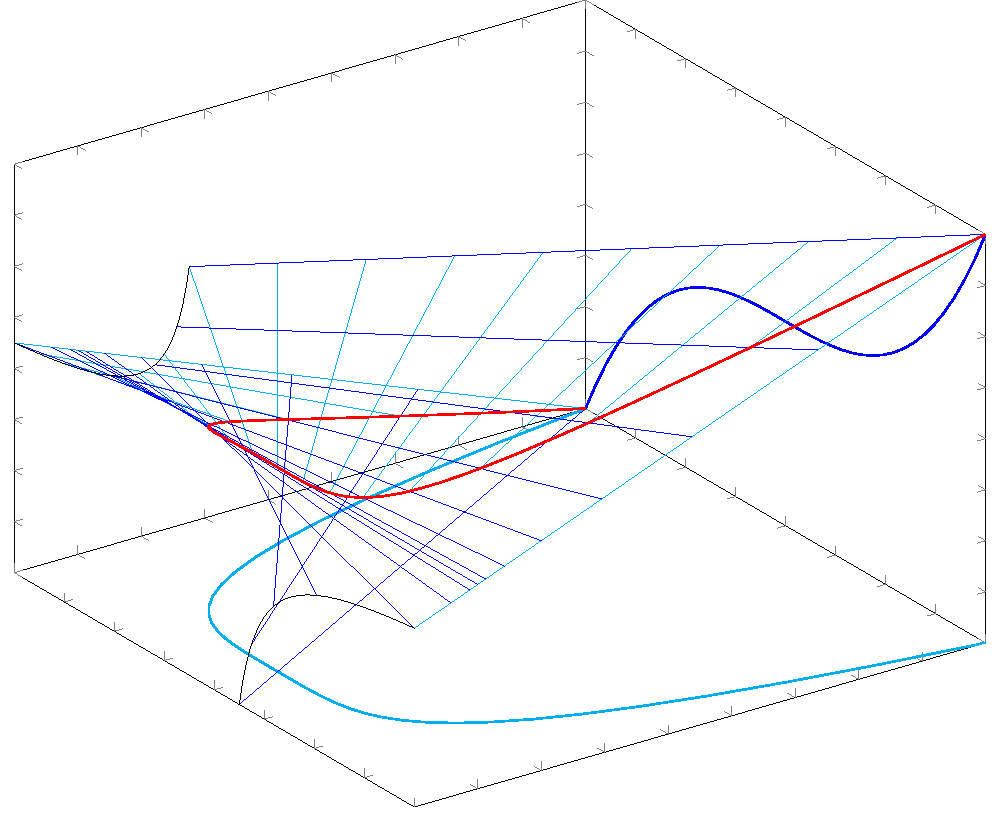
\includegraphics[scale=0.6,angle=74]{main/Fig03-newfigg}}\vskip-20pt}\hskip-50pt
%
\rlap{\hskip6pt\raise150pt\hbox{$z$}}%
\rlap{\hskip1.5pt\raise116pt\hbox{$_0$}}%
\rlap{\hskip1.5pt\raise191pt\hbox{$_{8}$}}%
\rlap{\hskip1pt\raise267pt\hbox{$_{16}$}}%
%
\llap{\raise37pt\hbox{$x$}\hskip40pt}%
\llap{\raise2pt\hbox{$_{-2}$}\hskip89pt}%
\llap{\raise24pt\hbox{$_{-1}$}\hskip66pt}%
\llap{\raise47pt\hbox{$_0$}\hskip44pt}%
\llap{\raise70pt\hbox{$_1$}\hskip20pt}%
\llap{\raise92pt\hbox{$_2$}\hskip-2pt}%
%
\llap{\raise11pt\hbox{$y$}\hskip167pt}%
\llap{\raise32pt\hbox{$_8$}\hskip210pt}%
\llap{\raise24pt\hbox{$_4$}\hskip182pt}%
\llap{\raise16pt\hbox{$_0$}\hskip152pt}%
\llap{\raise8pt\hbox{$_{-4}$}\hskip124pt}%
\llap{\raise1pt\hbox{$_{-8}$}\hskip98pt}%
%
\llap{\raise150pt\hbox{\rotatebox{73}{$_{y@=@8}$}}\hskip151pt}%
\llap{\raise162pt\hbox{\rotatebox{-72}{$_{x@=@2}$}}\hskip55pt}%
\llap{\raise267pt\hbox{$_{y@=@x^3}$}\hskip69pt}%
\llap{\raise116pt\hbox{\rotatebox{73}{$_{z@=@x^{@4}}$}}\hskip19pt}%
\llap{\raise73pt\hbox{\rotatebox{-27}{$_{z@=@-2}$}}\hskip153pt}%
\llap{\raise96pt\hbox{\rotatebox{50}{$_{z@=@-2}$}}\hskip44pt}%
%
\caption{A rational quartic space curve of type $(1,3)$ on a quadric
  surface. The quartic, in red, is given by $t\mapsto (t,t^3,t^4)$,
  and so projects to the cubic and quartic curves in the
  $xy$- and $xz$-planes (shown on the top and right surfaces of the
  box). The quartic, $z=xy$, is illustrated by means of its rulings
  and its intersections with the bounding planes. (Inspired by code of
  Enrique Acosta Jaramillo for the twisted cubic.)
\index{Acosta Jaramillo, Enrique}%
}
\end{figure}

\subsection*{Some open problems about rational curves}

We can say far less about rational curves of higher degree, even in $\PP^3` `$. For example, when $d$ is large, we
don't know the possible Hilbert functions for curves of degree $d$ in $\PP^3` `$, and the situation in $\PP^r$ for
$r>3$ is even worse. However, we do know the Hilbert function of a \emph{general} rational curve $C \subset \PP^r$ of degree $d$.

Since such statements will come up often, we pause to explain
exactly what it means to say
\index{general@a general X has property Y}%
``A general X has property Y.'' This
statement presupposes a choice of a parameter space for objects of
type X,
that is to say, an algebraic variety $Z$ whose points each correspond to an object of type X. Thus, to be precise, the statement should be,
``An  object of type X that is general with respect to parameter space $Z$ has property Y.'' The statement then means: inside $Z$ there is
a dense open set whose elements correspond to objects of type X that have property Y. Often $Z$ is irreducible, and
then it is enough to have a nonempty open set, since every such set is Zariski dense.

In the case of nondegenerate rational curves
of degree $d$ in $\PP^{r}$
we could take for $Z$ the space of
$(r@{+}1)$-tuples of independent elements of $H^{0}(\op1d)$, or
equivalently, taking the quotient by $\PGL(r+1)$,
the
Grassmannian
\index{Grassmannian}%
 of $(r@{+}1)$-dimensional planes in $H^{0}(\op1d)$.
We will later make statements about general curves of genus $g$, referring either to
a component of a Hilbert scheme
(discussed in Chapter \ref{ModuliChapter}) or to the
moduli space of curves that is discussed at length in Chapter
\ref{CurvesModuliChapter}.

As in Proposition~\ref{ideal of rational quartic}, knowing the Hilbert function of a curve $C\subset \PP^{r}$ is tantamount to knowing the ranks of the restriction maps
$$
\rho_m : H^0(\cO_{\PP^r}(m)) \to H^0(\cO_C(m)) = H^0(\cO_{\PP^1}(md)).
$$
Equivalently we ask: if $V$ is a general  $(r+1)$-dimensional vector space of homogeneous polynomials of degree $d$, what is the dimension of the space of polynomials spanned by $m$-fold products of polynomials in $V$?

We might guess that the answer is, ``as large as possible,'' meaning
that the rank of $\rho_m$ is $\tbinom{m+r}{r}$ or $md+1$,
whichever is less
\emdash in
other words, the map $\rho_m$ is either injective or surjective for
each $m$. This was proved in \cite{Ballico-Ellia83}, and is a special
case of Larson's maximal rank theorem \cite{Larson}.

As we will see in subsequent chapters it is possible to speak of a
\index{general curve of genus $g$}%
general curve of genus $g$
and a
\index{general invertible sheaf}%
general invertible sheaf
of degree $d$ on such a curve; and the analogous statement
about Hilbert functions  was proven in \cite{Larson}; 
see Chapter~\ref{Brill--Noether}.

Nevertheless, even the degrees of the generators of the homogeneous ideal of a general
rational curve of degree $d$ in $\PP^3$ is unknown for larger $d$.

\subsubsection*{The secant plane conjecture}

If $C \subset \PP^r` `$, then an $e$-secant $s$-plane to $C$ is an
$s$-plane $\Lambda \cong \PP^s \subset \PP^r$ such that the
intersection $\Lambda \cap C$ has degree $\geq e$.
\index{secant plane conjecture}%

Should you expect a curve $C \subset \PP^r$ to have any $e$-secant
$s$-planes? The set of $s$-planes in $\PP^r$ is parametrized by the
Grassmannian
\index{Grassmannian}%
$\GG = \GG(s,r)$, which has dimension $(s+1)(r-s)$. Inside $\GG$, the locus of planes that meet $C$ has codimension $r-s-1$ (reason: the locus of planes containing a given point $p$ is isomorphic
by projection from $p$ to $\GG(s-1,r-1)$, and thus has codimension $r-s$).
Thus one might conjecture that a curve $C \subset \PP^r$
will have $e$-secant $s$-planes when
\vspace*{-3pt}
$$
e \; \leq \; (s+1)\frac{r-s}{r-s-1},
$$
perhaps with a few low-degree exceptions. Is this true of a general rational curve? For most $e$, $r$ and $s$, we don't know.

\section{The Cohen--Macaulay property}\label{ACM}

In Section~\ref{rational normal curves section} we defined a curve
$C\subset \PP^{r}$ to be arithmetically Cohen--Macaulay (ACM) if the
\index{Cohen--Macaulay}%
natural maps
$$
\rho_m: H^0(\sO_{\PP^r}(m)) \to H^0(\sO_{C}(m))
$$
are surjective for all $m$. When this is the case we can accurately predict the number of independent forms of
each degree vanishing on the curve, and the condition has other important consequences that we will explore here and in Chapters~\ref{LinkageChapter} and \ref{SyzygiesChapter}. For general treatments of
Cohen--Macaulay rings see \cite[Chapter 18]{Eisenbud1995} or the book \cite{BrunsHerzog}. One of the characterizations of the condition is in terms of regular sequences:
\index{regular!sequence}%

\begin{definition}\label{gradeDef}
A sequence of elements $f_{1}, \dots, f_{c}$ in a ring $R$ is
\emph{regular}
if
$f_{i+1}$ is a nonzerodivisor modulo $(f_{1}, \dots, f_{i})$ for $i = 0,\dots, c-1$ and the ideal
$(f_{1}, \dots, f_{c})$ is not the unit ideal.

The
\emph{grade}
\index{grade!of an ideal}%
of an ideal $I$ in a ring  $R$ (sometimes called the
depth
\index{depth!of an ideal}%
of $I$ on $R$) is the maximal length of a regular sequence contained
in $I$, or $\infty$ if $I = R$.

A local ring $(R,\gm)$ is \emph{Cohen--Macaulay} if $\grade \gm = \dim
R$.
A Noetherian ring
$R$ is called Cohen--Macaulay if
every localization is Cohen--Macaulay.
Likewise,
a scheme is Cohen--$`$Macaulay if
all its local rings are Cohen--Macaulay.
\end{definition}

\begin{example}
\begin{itemize}
 \item The sequence of elements $x_{0},\dots, x_{r}\subset S\colonequals \CC[x_{0}\dots, x_{r}]$ is regular, proving
 from the definition that the localization of $S$ at the homogeneous maximal ideal is Cohen--Macaulay.

 \item
Regular local rings
\index{regular!local ring}%
are Cohen--Macaulay. Thus every
smooth scheme
\index{smooth!implies Cohen--Macaulay}%
is Cohen--Macaulay, and in particular
$S\colonequals \CC[x_{0}\dots, x_{r}]$ is Cohen--Macaulay.

 \item It follows from the definition that any
\index{complete intersection}%
complete intersection in a Cohen--Macaulay scheme is again Cohen--Macaulay.
Thus every plane curve, and more generally every complete intersection curve,
\index{ACM}%
is ACM; and we shall show in Section~\ref{CastelnuovoSection} that every canonically embedded curve
and every curve embedded by a complete linear series of sufficiently high degree is also ACM.

\item
Zero-dimensional rings
are all Cohen--Macaulay. The set of
zerodivisors in a Noetherian ring is the union of the
\index{associated prime}%
\index{prime!associated}%
associated primes of 0, so a
1-dimensional ring
is Cohen--Macaulay if and only if
\index{zero-dimensional ring}%
\index{1-dimensional ring}%
it is pure-dimensional (sometimes called
``unmixed'')
\emdash that is,
\index{unmixed ring}%
\index{pure-dimensional}%
every associated prime ideal is 1-dimensional.
Thus any purely 1-dimensional scheme is Cohen--Macaulay.
\end{itemize}
\end{example}

\begingroup \manyfacts
\begin{fact}
 \item We defined the
\index{grade}%
grade as the maximal length of a regular sequence in $I$; but in fact
all
\index{maximal regular sequence}%
maximal regular
sequences have the same length, equal to the smallest integer $k$ such that
$\smash{\Ext^{k}(R/I,R)}\neq 0$
\cite[Theorem 17.4 and Proposition 18.4]{Eisenbud1995}.

\item For any proper ideal $I\subsetneq R$ we have $\grade I \leq \codim I$. On the other hand, if $R$ is Cohen--Macaulay,
then $\grade I =\codim I$ for every ideal $I$ of $R$. In this sense the grade is an arithmetic
approximation to the codimension.

\item Every localization of a Cohen--Macaulay ring is Cohen--Macaulay. If $X\subset \PP^{r}$
has homogeneous coordinate ring $R_{X}$, then we say that $X\subset \PP^{r}$ is
arithmetically Cohen--Macaulay
\index{ACM!variety}%
if $R_{X}$ is Cohen--Macaulay, a property that depends on the
embedding, and implies the intrinsic property that $X$ is Cohen--Macaulay (since the local rings
of $X$ are essentially localizations of $R_{X}$). Previously we defined a curve $C\subset \PP^{r}$
to be arithmetically Cohen--Macaulay if the natural map $R_{C}\to H^{0}_{*}(\sO_{C})$ is surjective.
We will prove that this is equivalent to $R_{C}$ being Cohen--Macaulay in Proposition~\ref{ACM basics}. The same definitions and theorem apply to a positively graded ring, and homogeneous ideals.

\item By
Serre's criterion
\index{Serre's criterion}%
\cite[Section 11.2]{Eisenbud1995} the homogeneous coordinate ring
$R_C$ of a curve $C$ is
normal
\index{normal!ring}%
(that is, integrally closed)
if and only if
$C$ is both nonsingular and ACM, and sometimes $C$ is said to be
\index{projectively normal}%
\emph{projectively normal} in this case.  (This is also the excuse for
the terminology
``linearly normal''
\index{linearly normal}%
\index{quadratically normal}%
for a curve embedded by a complete linear series,
quadratically normal
if $\rho_{2}$ is surjective, and so on.)
\end{fact}
\endgroup

\vspace*{3pt}

\begin{proposition}\label{ACM basics}
Suppose that $C\subset \PP^r$ is a 1-dimensional subscheme. Let $S = H^0_*(\sO_{\PP^r})$
be the homogeneous coordinate ring of $\PP^r` `$, and let $R_C = S/I_C$ be the homogeneous
coordinate ring of $C$. The following conditions are equivalent:
\vadjust{\goodbreak}%
\begin{enumerate}

 \item The natural injective map $R_C \to H^0_*(\sO_{C}(1))$ is surjective.

\item $H^1_*(\sI_{C/\PP^r}) = 0$.

\item The homogeneous coordinate ring $R_C$ of $C$ is a Cohen--Macaulay ring; that is, there are linear forms $h,h'$ on $\PP^r$ whose images in  $R_C$ form a regular sequence. In particular, $R_C$ has no $0$-dimensional primary components,
so $C$ is purely $1$-dimensional and thus Cohen--Macaulay as a scheme.
\index{Cohen--Macaulay!scheme}%

 \item For every hyperplane $H\subset \PP^r$ that does not contain any component of $C$,
 the homogeneous ideal of $H\cap C$
 is equal to  $I_C+(h)$, where $h$ is a linear form defining $H$.
\end{enumerate}
\end{proposition}

\begin{proof}
\def\sl#1{(#1)}
\let\rTo\to
\let\Leftrightarrow\iff
{\sl 1} $\Leftrightarrow$ {\sl 2}: We may assume that $r\geq 2$, so $H^1_*(\sO_{\PP^r}(n)) = 0$ for all $n$. Using this and the exact sequence
$
0\rTo \sI_{C/\PP^r}  \rTo  \sO_{\PP^r}  \rTo  \sO_C  \rTo  0
$
we see that $H^0(\sO_{\PP^r}(n)) \to H^0(\sO_C(n))$ is surjective for all $n$ if and only if $H^1(\sI_{C/\PP^r}(n)) = 0$ for all $n$,
proving the equivalence of {\sl 1} and {\sl 2.}

{\sl 1} $\Leftrightarrow$ {\sl 3}: First let $C\subset \PP^r$ be an arbitrary 1-dimensional subscheme,
and let $R =H^0_*(\sO_{C}) \colonequals \bigoplus_{n\in \ZZ} H^0(\sO_{C}(n))$.
If $H$ is a
general hyperplane, with equation $h=0$, then $h$ does not vanish on any primary component of $C$, and thus the sequence
$$
0\rTo \sO_C(-1) \ruto{\ h}\sO_C\rTo \sO_{C\cap H}\rTo 0
$$
is exact. Applying $H^0_*$ and using
(2),
we see that $h$ is a nonzerodivisor on $R$, and that $R/hR$ is
a subring of $H^0_*(\sO_{C\cap H})$.  A general linear form $h'$ doesn't vanish on
any point of $C\cap H$, so $h'$ is a unit on $H^0_*(\sO_{C\cap H})$
and thus a nonzerodivisor on $R/hR$.

The ring $R_C$ is the image of the natural map $S\to R$, and by definition $C$ is ACM if and only if this map is surjective,
so that $R_C = R$. This shows that if $C$ is arithmetically Cohen--Macaulay then $R_C$ is a Cohen--Macaulay ring,
and is in particular unmixed; that is, $C$ has no 0-dimensional primary components (see for example \cite[Chapter 18]{Eisenbud1995} for general
information about Cohen--Macaulay rings). This proves the equivalence of conditions {\sl 1} and {\sl 3.}


{\sl 3} $\Leftrightarrow$ {\sl 4}: If  $h$ does not vanish on any component of $C$ then $h$ is a nonzerodivisor on $R_C$. The ideal $I_{C\cap H}$ is in any case the saturation of $I_C+(h)$.
If $I_{C\cap H}=I_C+(h)$, then any linear form $h'$ not containing a point of $C\cap H$ is a nonzerodivisor
on $I_C+(h)$, so $C$ satisfies condition {\sl 2}. Conversely, in a 2-dimensional positively graded Cohen--Macaulay ring, any
series of parameters is a regular sequence \cite[Section 18.2]{Eisenbud1995}, so $I_C+(h)$ is unmixed, and in particular, saturated.
\end{proof}

\begin{fact}\label{meaning of ACM}
The Cohen--Macaulay property is hard to interpret geometrically; the definition is justified by its usefulness. Here are two results that help our intuition:
\begin{enumerate}
\item A scheme $X$ is Cohen--Macaulay if some (equivalently every) finite map $f: X\to P$ to a smooth scheme $P$
of the same dimension is
\index{flat map}%
flat, or equivalently the pushforward $f_*(\sO_X)$ is locally free. (This follows
from the
Auslander--Buchsbaum formula
\index{Auslander--Buchsbaum formula}%
\cite[Section 19.3]{Eisenbud1995}.)
\item (Hartshorne) If a scheme $X$ is Cohen--Macaulay then $X$ is
\index{connected in codimension 1}%
connected in codimension 1
(that is, $X$ remains connected after removing any
closed subset of codimension $\geq 2$).
See
\cite[Theorem 18.12]{Eisenbud1995} for a proof.
\vspace*{-1.4\baselineskip}
\end{enumerate}
\end{fact}

\section{Exercises}

\begin{exercise}\label{1,d-1 on quadric}
Let $\sV =(\sO_{\PP^1}(d), V)$ be the linear series of degree $d$ on $\PP^1$ defined by the vector space
$V = \langle s^{d},s^{d-1}t, st^{d-1}, t^d\rangle$, where $s,t$ are coordinates on $\PP^1` `$. Show that $\sV$ defines
an isomorphism from $\PP^1$ onto a smooth curve
of type $(1,d{-}1)$ on a quadric surface.
\tohint{3.1}
\end{exercise}

\begin{exercise}\label{veronese inverse}
With notation as in Section~\ref{rational normal curves section}, show that the sheaf associated to the graded module $\coker M$,
that is, the cokernel of the map $\sO_{\PP^d}^d(-1) \to\nobreak
\sO_{\PP^d}^2$ defined by $M$, is the unique invertible sheaf of degree 1
on the rational normal curve $C$, and that thus the associated complete linear series defines the isomorphism $C\to \PP^1$ inverse
to the
Veronese map.
\index{Veronese!map!equation of}%
\end{exercise}

\begin{exercise}\label{equations of Veroneses}
Considering $\PP^n$ as $\Proj \CC[x_0,\dots,x_n]$, we may index the
variables
of $\PP^{\sbinom{n+d}{d}-1}$ by  monomials $p$
of degree $d$ in the $x_i$. Let $M_{n,d}$ be an $(n{+}1)\times \tbinom{n+d-1}{n}$ matrix
whose rows are indexed by the variables $x_i$, whose columns are indexed by the monomials $m$ of degree $d-1$ in the $x_i$ and
whose $(i,m)$ entry is the variable corresponding to the monomial $x_im$. (The matrix
$M$ of Section~\ref{rational normal curves section} is $M_{1,d}$.)
Show that the $2\times 2$ minors of $M_{n,d}$ generate the ideal of the image $V_{n,d}$ of the Veronese map
$\PP^n\to \PP^{\sbinom{n+d}{d}-1}$, and that the cokernel of $M_{n,d}$ is the unique invertible sheaf of degree 1 supported on $V_{n,d}$.
\end{exercise}

\begin{exercise}
 Let $\nu_d: \PP^r \to \PP^{\sbinom{r+d}{r}-1}$ be the $d$-Veronese
 map, and let $C\subset \PP^r$ be the
rational normal curve
\index{rational!normal curve}%
of degree $r$. Is $\nu_d(C)$ nondegenerate? If not, what is the dimension of its linear span (that is, of the smallest linear
 space that contains it)?
\tohint{3.4}
\end{exercise}

\begin{exercise}\label{arbitrary hyperplane examples}
Let $C_1$ be the union of two
\vadjust{\allowbreak}%
skew lines
\index{skew lines!in $\symbb P^3$}%
in $\PP^3` `$, and let $C_2$ be the
double line
\index{double line on a quadric}%
on a smooth quadric in $\PP^3` `$.
Show that a general hyperplane section of $C_1$ and of $C_2$  violates the conclusion of Proposition~\ref{arbitrary hyperplane}.
\end{exercise}

\begin{exercise}\label{restriction of ideals}
Suppose that $X\subset \PP^r$ is a subscheme and  $Z$ is the hypersurface in $\PP^r$ defined by a polynomial $F\in H^0(\sO_{\PP^r}(m))$. If the restriction of $F$ is a nonzerodivisor in
$\sO_X(m)$  then there is a short exact sequence
\index{restriction of ideals}%
$$
\sI_X(d-m) \ruto {\ F} \sI_X(m) \to \sI_{X\cap Z}(m) \to 0.
$$
\end{exercise}

\begin{exercise}\label{bad restriction}
Let $C\subset \PP^3$ be the smooth rational quartic
\index{rational!quartic}%
(or any smooth curve embedded by an incomplete linear series), and let
$h$ be a linear form defining a hyperplane $H$.
Show that
the  irrelevant ideal is associated to the
homogeneous ideal $I_C+(h)$, and thus $I_C(1)/hI_c$ is not the saturated homogeneous ideal of the finite
set $C\cap H$.
\end{exercise}

\begin{exercise}
Show that the
twisted cubic
\index{twisted cubic!as intersection of 3 quadrics}%
is the unique irreducible, nondegenerate space curve lying on three quadrics by considering the possible
intersections of two of the quadrics. \tohint{3.8}
\end{exercise}

\begin{exercise}\label{decomposition of a $g^3_4$}
As a consequence of our description of
rational quartic
rational quartic curves on a smooth quadric in Proposition~\ref{ideal of rational quartic},
show that a general $g^3_4$ on $\PP^1$ is uniquely expressible as a sum of the $g_1^1$ and a $g^1_3$
(in other words, a general 4-dimensional vector space of quartic polynomials on $\PP^1$ is uniquely expressible as the product of a 2-dimensional vector space of cubics and the 2-dimensional space of linear forms.
\tohint{3.9}
\end{exercise}

\begin{exercise}\label{distinguishing rational quartics}
Show that, up to projective equivalence, there is a 1-parameter family of embeddings of $\PP^1$ as a
smooth quartic curve in $\PP^3$
by constructing an invariant that distinguishes them.
\tohint{3.10}
\end{exercise}

\begin{exercise}\label{Castelnuovo uniqueness}
Complete the proof of Proposition~\ref{points on rnc} by showing that
if $C, C'$ are two rational normal curves in $\subset \PP^n$
meeting in at least $n+3$ distinct points, then $C = C'$.
\tohint{3.11}
\end{exercise}

\begin{exercise}\label{rnc and representations}
Let $V = \CC\cdot e_1\oplus \CC\cdot e_2$ be a 2-dimensional vector space.

The group $\SL_2= \SL (V)$ acts on the
rational normal curve
\index{rational!normal curve}%
of degree $d$ through automorphisms induced from its action on
\index{SL@$\SL_n, \,\SL(V)$, representation theory of}%
\index{Sym@$\Sym$, $\Sym^i$}%
the ambient space $\PP^d$ of the rational normal curve, which may be identified with $\PP(\Sym^d(V))$.

In \cite[pp.\,146--150]{Fulton-Harris} it is shown that
 every finite-dimen\-sional rational
representation of $\SL(V)$ is a direct sum of representations of the
form $\Sym^e(V)$ for various $e\geq 0$.
There it is explained that to understand how a given representation decomposes one should look at the action of the
torus generator
\index{torus generator}%
$$
\alpha \colonequals \biggl(\begin{matrix}
t&0\\
0&t^{-1}
\end{matrix}
\biggr)
\in \SL(V).
$$
The eigenvectors of $\alpha$ are called the {\it weight vectors} of the representation.
\index{weight}%
Note that $\Sym^e(V)$ is spanned by the weight vectors
$w_s \colonequals e_1^{e-s} e_2^{s}$
that satisfy $\alpha w_s = t^{e-2s}$ for $s = 0, \dots e$.
To decompose an arbitrary representation $W` `$, knowing that $W$ is a direct sum of $\Sym^{e_i}V` `$, it is enough to know the
\index{Sym@$\Sym$, $\Sym^i$}%
eigenvalues for the action of $\alpha$: We begin by finding an element $w\in W$ that
is an eigenvector of $\alpha$ and transforms by $\alpha$ as $\alpha w
= t^mw$ with the highest possible $m$ (this is called a ``highest
weight vector'').
Such a $w$
must be contained
in a summand $\Sym^m(V)$, and after removing the eigenvalues of the action of $\SL_2$ on $\Sym^m(V)$, we continue.
\begin{enumerate}
 \item Use this method to show that
\index{Sym@$\Sym$, $\Sym^i$}%
\begin{align*}
 \Sym^d(V)\otimes \Sym^d(V)&= \Sym^{2d}(V) \oplus  \Sym^{2d-2}(V) \oplus \Sym^{2d-4}(V) \otimes\cdots,\\
 \Sym^2(\Sym^d(V))&= \Sym^{2d}(V) \oplus \Sym^{2d-4}(V)\oplus \Sym^{2d-8}(V)\otimes \cdots,\\[-1.5pt]
 \mwedge^2(\Sym^d(V))&= \Sym^{2d-2}(V) \oplus \Sym^{2d-6}(V)\oplus \Sym^{2d-10}(V)\otimes \cdots,
\end{align*}
where we take $\Sym^{m}(V)=0$ when $m<0$.
 \item Show that the space of quadrics containing the rational normal curve is a representation of $\SL_2$ of the form
 $$
 \Sym^{2d-4}(V)\oplus \Sym^{2d-8}(V) \cdots
 $$
  \item Show  there is a distinguished nonsingular
\index{skew-symmetric form}%
\index{twisted cubic}%
skew-symmetric form (up to scalars) on the ambient space of the twisted cubic.
Thus a twisted cubic in $\PP^3$ determines, for each point of $\PP^3` `$, a distinguished plane containing that point.
 \item Show that if $d$ is divisible by 4 there is a distinguished quadric in the ideal of the rational normal curve.
\end{enumerate}
\end{exercise}

\begin{exercise}\label{Normal bundle of cubic}
Let $\PP^1 \hookrightarrow C \subset \PP^3$ be a
twisted cubic.
\index{twisted cubic}%
Show that the normal bundle
\index{normal!bundle}%
$\cN_{C/\PP^3}$ (defined to be the quotient of the restriction
$T_{\PP^3}|_C$ to $C$ of the tangent bundle  of $\PP^3$  by the
tangent bundle $T_C$) is
$\cN_{C/\PP^3} \cong \cO_{\PP^1}(5) \oplus  \cO_{\PP^1}(5)$.
\tohint{3.13}
\end{exercise}

\begin{exercise}
Let $\PP^1 \hookrightarrow C \subset \PP^d$ be a rational normal
\index{rational!normal curve}%
curve. Show that the
normal bundle
\index{normal!bundle!of rational normal curve}%
$\cN_{C/\PP^d}$  is
\label{precex}
$$
\tsty
\cN_{C/\PP^d} \cong \bigoplus\limits_{i=1}^{d-1} \cO_{\PP^1}(d+2).
\tohint{3.14}
$$
\end{exercise}

\begin{exercise}
In the situation of
Exercise \ref{precex},
the set  of direct summands
of $\cN_{C/\PP^d} $ is a projective space $\PP^{d-2}$. How does the
group of automorphisms of $\PP^d$ carrying $C$ to itself act on this $\PP^{d-2}$?
\tohint{3.15}
\end{exercise}

See \cite{MR3778979}, for example,
\index{normal!bundle}%
\index{rational!curve}%
for more on normal bundles of rational curves.

\begin{exercise}\label{ci is acm}
If $C=\bigcap_{i = 1}^{r-1}X_i \subset \PP^r$ is a
\index{complete intersection}%
complete intersection
 of hypersurfaces,
then $C$ is
\index{ACM}%
arithmetically Cohen--Macaulay.
\tohint{3.16}
\end{exercise}

\begin{exercise}
Give a proof of Corollary~\ref{minimal degree bound} without using
Bertini's theorem, by projecting $X$ from a general point and using
induction on $\codim X$.
\tohint{3.17}
\end{exercise}


%header and footer for separate chapter files

\ifx\whole\undefined
\documentclass[12pt, leqno]{book}
\usepackage{graphicx}
\input style-for-curves.sty
\usepackage{hyperref}
\usepackage{showkeys} %This shows the labels.
%\usepackage{SLAG,msribib,local}
%\usepackage{amsmath,amscd,amsthm,amssymb,amsxtra,latexsym,epsfig,epic,graphics}
%\usepackage[matrix,arrow,curve]{xy}
%\usepackage{graphicx}
%\usepackage{diagrams}
%
%%\usepackage{amsrefs}
%%%%%%%%%%%%%%%%%%%%%%%%%%%%%%%%%%%%%%%%%%
%%\textwidth16cm
%%\textheight20cm
%%\topmargin-2cm
%\oddsidemargin.8cm
%\evensidemargin1cm
%
%%%%%%Definitions
%\input preamble.tex
%\input style-for-curves.sty
%\def\TU{{\bf U}}
%\def\AA{{\mathbb A}}
%\def\BB{{\mathbb B}}
%\def\CC{{\mathbb C}}
%\def\QQ{{\mathbb Q}}
%\def\RR{{\mathbb R}}
%\def\facet{{\bf facet}}
%\def\image{{\rm image}}
%\def\cE{{\cal E}}
%\def\cF{{\cal F}}
%\def\cG{{\cal G}}
%\def\cH{{\cal H}}
%\def\cHom{{{\cal H}om}}
%\def\h{{\rm h}}
% \def\bs{{Boij-S\"oderberg{} }}
%
%\makeatletter
%\def\Ddots{\mathinner{\mkern1mu\raise\p@
%\vbox{\kern7\p@\hbox{.}}\mkern2mu
%\raise4\p@\hbox{.}\mkern2mu\raise7\p@\hbox{.}\mkern1mu}}
%\makeatother

%%
%\pagestyle{myheadings}

%\input style-for-curves.tex
%\documentclass{cambridge7A}
%\usepackage{hatcher_revised} 
%\usepackage{3264}
   
\errorcontextlines=1000
%\usepackage{makeidx}
\let\see\relax
\usepackage{makeidx}
\makeindex
% \index{word} in the doc; \index{variety!algebraic} gives variety, algebraic
% PUT a % after each \index{***}

\overfullrule=5pt
\catcode`\@\active
\def@{\mskip1.5mu} %produce a small space in math with an @

\title{Personalities of Curves}
\author{\copyright David Eisenbud and Joe Harris}
%%\includeonly{%
%0-intro,01-ChowRingDogma,02-FirstExamples,03-Grassmannians,04-GeneralGrassmannians
%,05-VectorBundlesAndChernClasses,06-LinesOnHypersurfaces,07-SingularElementsOfLinearSeries,
%08-ParameterSpaces,
%bib
%}

\date{\today}
%%\date{}
%\title{Curves}
%%{\normalsize ***Preliminary Version***}} 
%\author{David Eisenbud and Joe Harris }
%
%\begin{document}

\begin{document}
\maketitle

\pagenumbering{roman}
\setcounter{page}{5}
%\begin{5}
%\end{5}
\pagenumbering{arabic}
\tableofcontents
\fi


\chapter{Smooth plane curves and curves of genus 1}\label{3b}\label{genus 1 chapter}

If $C$ is a curve of genus 1, then by Corollary~\ref{degree 2g+1 embedding}, any complete linear series $D$ of
degree $3 = 2g+1$ on $C$ is very ample. By the Riemann--Roch theorem any invertible sheaf
of degree $d>0$ on $C$ has $d$ sections, so the morphism associated to $D$ embeds $C$
as a plane curve of degree 3, on which $D$ is the intersection of $C$ with a line. 

We therefore begin this chapter with a general explanation of sheaves of differentials and linear
series on smooth plane curves, and use that theory to say a little about other embeddings of 
curves of genus 1. Though most curves cannot be realized as smooth plane curves, we shall see
in Proposition~\ref{nodal projection} that every curve can be projected birationally to a plane curve whose only singularities are ordinary nodes, and in Chapter~\ref{PlaneCurvesChapter} we will
explain the analogous treatment of differentials and linear series on such nodal curves, and more
generally---but with less specificity---on all reduced plane curves.

Using the plane model of a curve of genus 1, we shall see  that the theory  is only a little more complicated than for genus 0 (but curves of genus 1 over number fields occupies a major part of modern number theory!)  


\section{Riemann, Clebsch, Brill and Noether}
For a long time, plane curves were the only algebraic curves that were studied. Originally these were curves in the affine plane over the real numbers, but by the second half of the 19th century the complex projective plane was well understood, and curves in $\PP^2 = \PP^2_\CC$, corresponding to irreducible forms in 3 variables, were recognized as the natural objects of study---see the historical appendix to this book for more details.

The work of Bernhard Riemann dramatically changed the focus of the theory to branched coverings of   the ``Riemann Sphere'' ($\PP^1_\CC$). The Riemann--Roch theorem, in particular, gave information about the existence of meromorphic functions on such coverings, well beyond what could be done in the earlier theory. However, Riemann's work, depending as it did on the then-obscure ``Dirichlet principle'', was not universally accepted. In the 1860s Alfred Clebsch and, after the death of Clebsch  in 1872, Alexander Brill and Max Noether (Emmy Noether's father), undertook the ambitious program of redoing the Riemann--Roch theorem entirely in terms of plane curves. They went beyond Riemann in certain directions, too: the Brill-Noether theorem treated in our Chapter~\ref{Brill-Noether} was formulated by Brill and Noether, and ``proved'' by them through an unsupported general position assumption. 

A central difficulty in the Brill-Noether attempt on the Riemann--Roch theorem was that,
although any smooth curve can be embedded in $\PP^r$ for any $r \geq 3$, most curves cannot be embedded in the plane. 
However, as is shown in Section~\ref{good projections}, we can embed $C$ as a curve $ C \subset \PP^r$ in a higher-dimensional projective space and find a projection $\PP^r \to \PP^2$ that carries $C$ birationally onto its image $C_0$, called a plane model of $C$. The curve $C_0$ typically has singularities, and $C$ is the normalization of $C_0$. Brill and Noether wanted to prove the Riemann--Roch theorem for $C$ by formulating and proving a related theorem for $C_0$. In particular, they tried to characterize linear equivalence of divisors on $C$ in terms of certain ``clusters'' of points---we would say 0-dimensional subschemes---of $C_0$. 

To carry out this program, a key step was to show that if $D\subset C_0$ is contained in the intersection
$D'$ of $C_0$ and some other plane curve $C_0'$, then a divisor 
$E := D'-D$ can be defined with properties such as that $D'-E = D$; Brill and Noether seem simply to have assumed that this is so. A bit later Frances Sowerby Macaulay proved that this is in fact possible  and also understood that it would not generally be possible if $D'$ were the intersection of three or more curves.\footnote{In modern terms, the intersection of two curves is Gorenstein; the intersection of 3 is generally not.}

Macaulay exploited this theory of residuation  to prove what he called the ``Generalized Riemann--Roch theorem'' Theorem~\ref{CBM}. This early work of Macaulay led directly to his definitions of  ``perfection'' (a homogeneous ideal
$I  \subset S:= k[x_0, \dots, x_n]$ is perfect if $S/I$ is Cohen-Macaulay) and ``super-perfection'' (the case when $S/I$ is
Gorenstein). For all this, see~\cite{eisenbud-gray}.

In this section we will take the point of view of Clebsch, Brill and Noether, and explain how to understand 
the differential forms and, given a (possibly ineffective) divisor $D$ on $C$, how to find all the 
effective divisors on $C$ that are linearly equivalent to $D$, in terms of a smooth plane curve. In Chapter~\ref{PlaneCurvesChapter} we will return to this point of view and treat the case of
nodal curves and the case of arbitrary reduced plane curves. We will give effective algorithms for
two constructions:

\begin{enumerate}
\item Given the equation $F(X,Y,Z)$ of a smooth $d$ plane curve $C$
of degree $d$, we can
construct a basis for $H^0(K_C)$; and

\item  Given a possibly ineffective divisor $D = D_{+}-D_{-}$ on $C$ we can construct the complete linear series $|D|$ on $C$. In particular we can:
\begin{enumerate}
\item determine whether $D$ is equivalent to any effective divisor on $C$; and if so,
 \item find all effective divisors $E$ on $C$ with $E \sim D$; also,
 \item find a basis of $H^0(\cO_C(D))$, expressed in terms of curves of high degree with  base locus.
 \item find the homogeneous coordinate ring of the morphism defined by $|D|$ or a subseries.
\end{enumerate}
\end{enumerate}

\section{Smooth plane curves}\label{smooth plane curves}

\subsection{Differentials on a smooth plane curve}\label{canonical series on smooth plane curves}

Let $C \subset \PP^2$  be a smooth plane curve, given as the zero locus of a homogeneous polynomial $F(X,Y,Z)$ of degree $d$. By the adjunction formula (Proposition~\ref{adjunction}) the canonical  divisors on $C$
are the intersections of $C$ with curves of degree $d-3$. In the spirit of Brill and Noether we
will make this explicit by constructing all
 the regular differential forms on $C$ in terms of forms of degree $d-3$.


For this purpose we introduce coordinates $x = X/Z$ and $y = Y/Z$ on the affine open subset $U \cong \AA^2$ given by $Z \neq 0$, and let $f(x,y) = F(x, y,1)$ be the inhomogeneous form of $F$, so that $C^\circ = C \cap U$ is the zero locus $V(f) \subset  \AA^2$. 

Since an automorphism of $\PP^2$ can carry any point in $\PP^{2}$ to any other point, we may assume
that 
 the point $[0,1,0]$ (that is, the point at infinity in the vertical direction) does not lie on $C$ so that the
 projection  $\pi: C \to \PP^1$ from $(0,1,0)$, which is given by $[X,Y,Z] \mapsto [X,Z]$ (or, in affine coordinates, $(x,y) \mapsto x$)  has degree $d$. Let $D$ be the divisor defined by the intersection of $C$ with the line $Z=0$ at infinity.

Consider the
regular 1-form $dx$ on $\AA^2$, which we may regard as the pull-back of the form $dx$ on
 $\AA^{1}$.
Since the form $dx$ on $\PP^{1}$ has a double pole at infinity the form $dx|_{C}$ has polar
locus $2D$.
 
 \def\Co{{C^{\circ}}}
How do we get rid of the poles of $dx$? The extension to $\PP^2$ of a polynomial $h(x,y)$ of degree $m$ on
$\AA^2$ has a pole of order $m$ along the line $L$ at infinity. Thus if $h$ has degree at least 2 then $dx/h$ has no poles at infinity. However, $h(x,y)$ may well vanish at points of $\Co$, and this may create new poles of $dx/h$. Of course if $h$ vanishes only at  points of $\Co$ where $dx$ has a zero, the zeroes of $h$ may cancel the zeroes of $dx$ rather than creating new poles.
 
 To avoid producing new poles in this way we may take
 $$
 h(x,y) = f_{y} := \frac{\partial f}{\partial y}(x,y).
 $$
 We claim that 
 $$
\varphi_0 = \frac{dx}{f_{y}}
$$
is everywhere regular and nowhere 0 in $C^\circ$. 

Note that $df$ vanishes identically when restricted to $C^\circ$, so
 $$
 0 \equiv df|_{\Co} = f_{x}dx|_{\Co} + f_{y}dy|_{\Co} .
 $$
Clearly $\varphi_0$ is regular at points $p$ where
where $f_{y}(p) \neq 0$. At such a point, if $dx|_{\Co}$ were 0, then since $\Co$ is smooth we would have $dy|_{\Co} \neq 0$, contradicting the equation above. Thus $\varphi_{0}$ is both regular and nonzero at such points. On the other hand, if $f_{y}(p) = 0$, then since $\Co$ is smooth $f_{x}(p) \neq 0$, so $dx|_{\Co}$ and $f_{y}$ vanish to the same
order, whence, again, $\varphi_0 = (dx/f_{y})|_{\Co}$ is regular and nonzero, proving the claim.

Put differently, if $L$ is the line at infinity, so that $U = \PP^{2}\setminus L \cong \AA^{2}$,
then the cotangent bundle on $U$ is 
$\Omega_{U}=\sO_{U}dx \oplus \sO_{U}dy,$
so 
the cotangent bundle $\Omega_{\Co}$ on $C^{\circ}$, which is the canonical bundle $\omega_{\Co}$,
 is the cokernel of the map from the normal sheaf $\sO_{C}(-d)|_{U}$ to the restriction of 
$\Omega_{U}$ to $C^{\circ}$. This map sends the local generator $f$ of the normal sheaf to
$f_{x}dx+f_{y}dy \in \Omega_{U}$, and because $f_{x}$ and $f_{y}$ have no common zeros, the generator $d_{y} \in \Omega_{C^{\circ}}$ is a multiple of $dx/f_{y}$.
Thus the free $\sO_{C^{\circ}}$-module $\omega_{C}|_{C^{0}}$ is generated by $dx/f_{y}$.

Since $f_{y}$ has degree $d-1$, the rational function $1/f_{y}$ vanishes to order $d-1$ on the line
at infinity, and thus in particular on the divisor $D$. Thus $\varphi_0$ vanishes to order $d-3$ on $D$; in other words, as divisors,
$$
(\varphi_0) = (d-3)D.
$$
In particular, if $d \geq 3$ then $\varphi_0$ is a globally regular differential on $C$. The divisor of
zeros of this differential has degree $d(d-3)$. If $g$ is the genus of $C$, then we must
have $2g-2 = d(d-3)$, whence 
$$
g = \frac{d(d-3)}{2} + 1 = \binom{d-1}{2}.
$$
We can produce a vector space of $\binom{d-1}{2}$ regular differentials by multiplying $\varphi_0$ by 
polynomials $e(x,y)$ 
  of degree $d-3$, since this does not introduce any poles. This proves:

\begin{theorem}
The space of regular differentials on a smooth plane curve $C$
with affine equation $f=0$ is 
$$
\left\{ \frac{e(x,y)dx}{f_{y}} \mid \hbox{ e(x,y) is a polynomial degree $\leq d-3$}\right\}.\qed
 $$
\end{theorem}

\subsection{Linear series on a smooth plane curve}\label{linear series on smooth plane curves}

Any divisor on a smooth plane curve $C$ may be expressed as the difference of
two effective divisors, $D= D_{+}-D_{-}$. We would like to find all the \emph{effective} divisors linearly equivalent to $D$, that is, of the form
$D + (H/G)$, where $G, H$ are forms of the same degree $m$. We begin by choosing
an integer $m$, large enough so there is a form $G$ of degree $m$ that vanishes on $D_{+}$ plus some divisor $A$ (but not on all of $C$). 

\begin{theorem}\label{equiv on smooth plane curve}
Let $D= D_{+}-D_{-}$ be a divisor on the smooth plane curve $C$. If
there is a form $G$ of degree $m$ vanishing on $D_{+}$ but not on all of $C$
then we may write $(G) = D_{+}+A$, and then
the effective divisors equivalent to $D$, if any, are precisely those 
of the form $(H) - A -D_{-}$ where $H$
is a form of degree $m$ vanishing on $D_{-}+A$, but not on all of $C$.
\end{theorem}

See Figure~\ref{Fig14.3} for an illustration with $D_+ = r+s+t, \ D_- = u$.
In particular, if no homogeneous polynomial $H$ of degree $m$ vanishes on  $A + D_{-}$ but not on $C$, then $D$ is not linearly equivalent to any effective divisor. The existence of such an $H$ is thus independent of the choices of $m$ and $G$, as we shall see in the proof.

The simplest special case of the theorem is the completeness of the linear series defined
by intersections of $C$ with curves of a given degree, 
or, equivalently, the fact that the restriction maps
$$
H^{0}(\sO_{\PP^{n}}(m)) \to H^{0}(\sO_{C}(m))
$$
are surjective for all $m$. 

\begin{proposition}\label {completeness of hyperplanes on plane curve}
If $C$ is a smooth plane curve, then any Cartier divisor on $D$ that is linearly equivalent to the divisor of
a form of degree $m$ is itself the divisor of a form of degree $m$; that is, plane curves are
arithmetically Cohen-Macaulay.
\end{proposition}

 The results for singular curves explained in Chapter~\ref{PlaneCurvesChapter}
 depend on strengthenings  of this condition.
 
\begin{proof}
Let $C$ be the plane curve defined by $F=0$, and let $D$ be the divisor on $C$ defined by a form $L$
of degree $m$, not vanishing on (any component of) the curve $C$. If $G$ and $H$ are forms of the same degree $t$, 
not vanishing on any component of $C$,
and $D+(G/H)$ is effective, then the divisor $(LG)$  on $C$ must contain the divisor $(H)$ on $C$.
This means that the subscheme of $\PP^{2}$ defined by $(LG,F)$ contains the scheme defined 
by $(H,F)$. Since $H$ and $F$ have no components in common, Theorem~\ref{Lasker} implies
that $LG = AH+BF$  for some forms $A,B$ with $\deg A = \deg LG -\deg H = m$ whence $D+(G/H) = (A)$
as required.
\end{proof}

\begin{example}
Suppose that $C$ has degree 3 and thus genus 1. If we choose as origin on the curve $C$ a point $o$, then to add two points $p$ and $q \in C$ means to find the (unique) effective divisor of degree 1 linearly equivalent to $p + q - o$. In this situation, Theorem~\ref{equiv on smooth plane curve} applies with $m=1$: there is a line $L$ 
containing $p+q$ defined by a linear form $G$. If $r \in C$ be the remaining point of intersection of $L$ with $C$ we can choose a linear form $H$ vanishing on $o+r$, and the line it defines meets $C$
in one additional point $s$. This is the classical construction of the group law on the points of $C$ (or,
for curves over a field that is not algebraically closed, on the rational points of $C$).
See Figure~\ref{group law on cubic}.
\end{example}

\begin{proof}[Proof of Theorem~\ref{equiv on smooth plane curve}]
First, suppose that we can find a form $H$ of degree $m$ as in the theorem.
Setting $D' = (H) -(D_{-}+A)$ we have
$$
D' = D + (H/G) = D_{+}- D_{-} - (D_{+}+A)+(D_{-}+A+D')
$$
so $D'$ is linearly equivalent to $D$. 

\begin{figure}
\centerline {\includegraphics[height=1.25in]{"main/Fig14-1"}}
\caption{If $G$ and $H$ have the same degree, then $r+s+t-u\sim p+q$ on $C$.}
\label{Fig14.3}
\end{figure}

We claim that we find in this way all effective divisors $D' \sim D$. 
To see this, suppose $D'$ is any effective divisor with $D' \sim D$, so that
$$
\cO_C(A+D_{-}+D') = \cO_C(A+D_{-}+D)  = \cO_C(m),
$$
that is, $A+D_{-}+D' \equiv (G)$ for some form $G$ of degree $m$. By Proposition~\ref{completeness of hyperplanes on plane curve}
this implies that $A+D_{+} = (H)$ for some form of degree $m$ as required.
\end{proof}


The argument given in Proposition~\ref{equiv on smooth plane curve} can be stated more generally thus:  if curves $F(X,Y,Z)=0$ and $Q(X,Y,Z)=0$ 
meet only in a finite set of points $\Gamma$ in $\PP^{2}$, and $E(X,Y,Z) = 0$ is a curve containing the intersection in an appropriate sense,
then $E = QH +LF$ for some forms $H$ and $L$, and this statement applies to arbitrarily singular curves. Recognizing its importance for the argument above and the generalizations to come, Max Noether in~\cite{Noether1873} dubbed it the \emph{Fundamental theorem}, 
noting that it had often been used by geometers but not proven. After successive attempts and 
criticisms involving many mathematicians, he and Brill gave a complete proof in~\cite{Brill-Noether}. For more of this story see the account in~\cite{eisenbud-gray}.

\subsection{The Cayley-Bacharach-Macaulay theorem}\label{CB section}

The following result was proven by Macaulay \cite[p.~424]{Macaulay1900}, as a version of the Riemann--Roch theorem. It is now widely referred to as the Cayley-Bacharach theorem, named for an
incorrect version asserted by Cayley and a correct special case later proven by 
Bacharach\cite{Bacharach1886}
; see \cite[Section 2.3]{eisenbud-gray} for more on this history, and 
\cite{MR1376653} (where the result is incorrectly attributed to Bacharach) for generalizations and related conjectures. Here is the version for divisors on a smooth plane curve:

\begin{theorem}[Cayley-Bacharach-Macaulay]\label{CBM} Let $C$ be a smooth plane curve of degree $d$, and suppose that
$E', E''$ are effective divisors on $C$ such that $E:=E'+E'' = C\cap C'$, the complete intersection of $C$
with a curve $C'$ of degree $d'$. For any integer $0\leq k \leq d+d'-3$, the difference in the number of conditions imposed 
on forms of degree $k$ by $E''$ and by $E$ is equal to the degree of $E'$ minus the
number of conditions $E'$ imposes on forms of degree $d'':=d+d'-3 -k$---that is, the ``failure of
$E'$ to impose independent conditions on forms of degree $d''$.

 Writing $H$ for
the divisor class on $C$ of the intersection of $C$ with a line, and setting $s := d+d'-3-k$ this is the equality:
$$
h^0(kH-E) - h^0(kH-E')  = \deg E'' - \left(h^0(sH) -  h^0(sH-E'')\right)
$$
\end{theorem}

\begin{proof}
Set $e' := \deg E', \ e'':= \deg E''$ and $e = e'+e'' = \deg E.$
By the adjunction formula, the divisor class of the canonical bundle on $C$ is $K = (d-3)H$. Using the Riemann--Roch theorem, the left hand side of the equality is
$$
kd-e-h^0(K - (kH-E)) - \left(kd-e' - h^0(K-(kH-E'))\right).
$$
Since $K - (kH-E) = K - (kH-d'H) = sH$ and  $K-(kH-E') = sH+E''$, we see that the 
left hand side is equal to 
$
e'' - h^0(sH) +  h^0(sH+E'')
$
as required.
\end{proof}

As noted in \cite{eisenbud-gray}, the converse, proving the Riemann--Roch theorem for $C$ from Theorem~\ref{CBM}, is also easy.

\begin{corollary}\label{CBM cor 1}
A divisor $E'$ on a smooth plane curve $C\subset \PP^2$ of degree $d$ moves
in a linear series of dimension $r$ if and only if $E'$ fails by $r$ to impose
independent conditions on curves of degree $d-3$.
\end{corollary}

\begin{proof}
For sufficiently large $d'$ we can choose a curve $C'$ of degree $d'$ containing
$E$ and meeting $C$ in $E = E'+E''$, where $E''$ is disjoint from $E'$. Since $C\cap C'$
is a complete intersection, every form vanishing on $E+E'$ is a linear combination of
the forms defining $C$ and $C'$, and thus the dimension of the space of forms of degree $d'$
vanishing on $E$ modulo those vanishing on $C$ is 1. By Theorem~\ref{equiv on smooth plane curve} the dimension $r$ of the linear series $|E'|$ is the dimension of the space of
forms of degree $d'$ modulo those vanishing on $E+E'$, and by Theorem~\ref{CBM} this
is the failure of $E'$ to impose independent conditions on forms of degree
$d'' = d+d' - d' -3 = d-3$.
\end{proof}

To apply Theorem~\ref{CBM} it is helpful to know when points impose independent conditions on forms of a certain degree. Here is a first result of this kind:

\begin{proposition}\label{n-2 independence}
Suppose that $1\leq n$. Any set $\Gamma$ of $k\leq n$ distinct points in $\PP^{2}$ imposes independent conditions on forms of degree $n-1$; and if $\Gamma$ is not contained in a line then $\Gamma$ imposes independent conditions on forms of degree $n-2$.
\end{proposition}

\begin{proof} To show that $\Gamma$ imposes independent conditions on forms of degree $d$ we must produce, for each $p\in \Gamma$, a form of degree $d$ vanishing on 
$$
\Gamma_{p}:=\Gamma\setminus\{p\}
$$
 but not $p$. If $\Gamma$ imposes independent conditions on forms of degree $d$ then
 $\Gamma$ automatically imposes independent conditions on forms of degree $d+1$,
 so we may assume that $k=n$.
 
The product of linear forms
 vanishing on general lines through the points of $\Gamma_{p}$ does not vanish at $p$, proving the first statement.

Now assume that $\Gamma$ is not contained in a line and $p\in \Gamma$. It suffices to show that for each $p\in \Gamma$ there is a form of degree $n-2$ vanishing on $\Gamma_{p}$ but not on $p$. Since $\Gamma$ spans $\PP^2$, there is a spanning set of three points $p,q,r$ of $\Gamma$. The union of the line spanned by $q,r$ with general lines through 
through the $n-3$ points of $\Gamma_{p}\setminus\{q,r\}$ is defined by a form of degree $n-2$ containing $\Gamma_{p}$ but not $p$, 
as required. 
\end{proof}

\begin{corollary}\label{CBM cor 2}
 Suppose that $C\subset \PP^2$ is a smooth plane curve of degree $d\geq 3$.
 
\begin{enumerate}
 \item If $\sV$ is a $g^1_e$ on $C$ with $e\leq d-1$ then $e = d-1$ and $\sV$
 corresponds to projection from a point of $C$.
 \item If $\sV$ is a $g^2_e$ on $C$ with $e\leq d \geq 4$ then $e = d$. Furthermore,  the
  embedding of $C$ in $\PP^2$ is unique up to automorphisms of $\PP^2$.
 \end{enumerate}
\end{corollary}

\begin{proof}
 1. If $E$ is a divisor in the linear series $\sV$ then by Corollary~\ref{CBM cor 1} the points of $E$ fail to impose
 independent conditions on forms of degree $d-3$. By Proposition~\ref{n-2 independence} the degree of $E$ is $d-1$
 and the points lie in a line $L$, which must meet $C$ in an additional point $p$. By Theorem~\ref{equiv on smooth plane curve}
 the linear series $|E|$ is residual to $p$ in curves of degree 1; that is, it is the linear series corresponding to projection from $p$.
 
 2. In this case a divisor in the series $\sV$ fails by 2 to impose independent conditions on forms of degree $d-3$, and
 thus fails (by at least 1) to impose independent conditions on forms of degree $d-2$. By 
  Proposition~\ref{n-2 independence} the degree of $E$ is $d$.
 Moreover, the points lie in a line $L$; thus $\sV$ is a subseries of the series by which $C$ is embedded.
 \end{proof}

\section{Curves of genus 1 and the group law of an elliptic curve}

We will describe the maps of a curve of genus 1 given by
the complete linear series in the lowest degree cases of interest: $d =  2, 3, 4$ and $5$. Along the
way we will see several ways of parametrizing the family of curves of genus 1 by one-dimensional varieties,
forerunners of the moduli spaces that we will introduce in Chapters~\ref{ModuliChapter} and~\ref{CurvesModuliChapter}.


On a smooth, irreducible curve $E$ of genus 1 the canonical sheaf has degree 0; and since it has a global section, it must be $\sO_C$.
Since invertible sheaves of negative degree cannot have any sections, the Riemann--Roch theorem shows that
$h^0( \sL) = \deg \sL$ for any $\sL$ of positive degree. Among the surprising consequences is that, given
a point $o\in E$, there is a natural structure of abelian algebraic group on the points of $E$ for which $o$
is the zero element. A curve of genus 1 with a chosen point $o$ is called an \emph{elliptic curve}.

\begin{proposition}\label{group law} Let $E$ be a curve of genus 1 and let $o$ be a chosen point $o\in E$.
If we set $p+q = r$ where $r$ is the unique effective divisor linearly equivalent to $p+q-o$, then $E$ becomes a
commutative algebraic group.
Moreover, the group of divisor classes is divisible, in the sense that for any divisor $D$ of degree $n>0$
 there is a point $p$ such that $D\sim np$.
 \end{proposition}

\begin{proof}
 The group operation is easy to describe:
Let $E$ be an elliptic curve with the point $o\in E$ chosen arbitrarily. If $p,q$ are points of $E$ then $\sO_E(p+q-o)$ has degree 1, and
thus has a unique global section. This vanishes at a unique point $r$, which may also be described as the unique
effective divisor linearly equivalent to $p+q-o$, and thus 
$p+q = r$ in the group operation, which is thus obviously commutative. For the inverse, if $r$ is the  unique point
linearly equivalent to $2o-p$ then $p+r-o\sim o$, so that $r=-p$. For any divisor $D$
we define $\Sigma D$ to be the unique point linearly equivalent to $\Sigma D-(\deg D-1)o$.
Note that in this group operation any two linearly
equivalent divisors have the same sum $\Sigma D = \Sigma D'$.

We can determine the point $r\sim p+q-o$ and show that the group law is given by regular functions
as follows. By Corollary~\ref{degree 2g+1 embedding} we may embed $E$ in $\PP^2$ by any linear series
of degree 3.  Let $L$ be the line through $p+q$, and suppose that
$L$ meets $C$ in an additional point $s$. Since $s$ is unique, its coordinates are polynomial functions
(on a suitable affine chart) of the coordinates of $p$ and $q$. The line through $s$ and $o$ meets $C$ additionally in a point $r$,
and by Theorem~\ref{equiv on smooth plane curve} we have $r\sim p+q-o$, as in Figure~\ref{group law on cubic}.
and similarly the point $r$ is a polynomial function of the coordinates of $s$ and $o$.

To see that $E$ is a divisible group, consider the maps $n: E\to E$ given by multiplication by integers $n$. Since the
group law is given by polynomial functions, the number of solutions $p$ of the equation $np = q$ is finite, and thus
for $n\neq 0$ this map is non-constant. This implies that it is surjective.
\end{proof}

It is convenient for some purposes to suppose that the linear series used to embed $C$ in $\PP^2$ is $|3o|$; this
has the advantage that $p,q,r\in C$ are colinear if and only if $p+q+r =o$ in the group law.

\begin{figure}
\centerline {\includegraphics[height=2.2in]{"main/Fig03-2"}}
 \caption{Adding points $p, q$ on a plane cubic with origin $o$
 {Silivo: please make the picture less symmetric: o should not be a flex point and p plays a role different from o.}}
\label{group law on cubic}\end{figure}

\begin{remark}
From the definition it is obvious that 
the map
$E \to \Pic_0(E)$ sending $p$ to $\sO_E(p-o)$ is an isomorphism of groups, and adding multiples of $o$
induces an isomorphism with each $\Pic_d(E)$ as well. This provides a natural sense
in which the family of invertible sheaves on $C$ can be treated as a smooth curve.
 In Chapter~\ref{JacobianChapter} we will see a general construction: the Picard group $\pic_0(C)$ can be made into
a variety, and for a curve $C$ of genus $g$ the effective divisors
of degree $g$ form a variety that surjects birationally to $\Pic_g(C)$. 
\end{remark}
 

\begin{corollary}\label{equivalence of sheaves}
Given two invertible sheaves $\sL, \sL'$ of the same degree on a curve $E$ genus 1, there is an automorphism $\sigma: E\to E$
such that $\sigma^*\sL = \sL'$.
\end{corollary}

\begin{proof}
By Proposition~\ref{group law} we may write $\sL \cong \sO_E(np)$ and $\sL'\cong \sO_E(np')$ for some points $p,p'$; and translation by $p-p'$
is an automorphism of $E$ carrying one into the other.
\end{proof}


\section{Low degree divisors on curves of genus 1} 

In this section we will describe the complete linear series of degrees 2,3,4, and 5 on a curve of genus 1, and say something
about the geometry of each case. Several of these descriptions lead to natural guesses answering the
apparently silly question: How many different curves of genus 1 are there? 

\subsection {The dimension of families}

To make sense of this question, we observe a fundamental fact of algebraic curve theory that the set of isomorphism classes of smooth, projective curves of a given genus $g$ is naturally parametrized by the points of a
an irreducible quasiprojective variety $M_g$, called the \emph{moduli space} of curves of genus $g$. We will have a great deal more to say about moduli spaces in general, and $M_g$ in particular, in Chapters~\ref{ModuliChapter} and~\ref{CurvesModuliChapter}. 

We will use the low degree embeddings  to describe the family of isomorphism classes of curves of genus 1 in several ways, giving
what seem to be natural estimates of its dimension. We leave to Chapter~\ref{CurvesModuliChapter} the reasoning that leads to a map from the base of such a family to $M_{1}$, validating the estimates we give here.

\subsection{Double covers of $\PP^1$}

Let $E$ be a smooth projective curve of genus 1 and let  $\sL$ be an invertible sheaf of degree 2 on $E$. By the Riemann--Roch theorem, $h^0(\sL) = 2$ and the linear series $|\sL|$ is base-point free, so we get a map $\phi : E \to \PP^1$ of degree 2. By the Riemann-Hurwitz theorem the map $\phi$ will have 4 branch points, which must be distinct because in a degree 2 map
only simple branching is possible. By Corollary~\ref{equivalence of sheaves}, this set of four points are determined, up to automorphisms of $\PP^1$, by the curve $E$, and are independent of the choice of $\sL$. 

%In terms of a given embedding of $E$ as a smooth cubic in $\PP^{3}$, Corollary~\ref{CBM cor 2}
%shows that the linear series corresponding to a map to $\PP^{1}$ of degree 2 are 
%projections from points of $E$, suggesting again that $M_{1}$ has dimension 1.

We will see in Chapter~\ref{genus 2 and 3 chapter} that a double cover of $\PP^1$ is determined by  its branch points, so the family $\cH$ of double covers of $\PP^1$ having genus 1 is four-dimensional. There is a map $\cH \to M_1$, sending such a double cover to the isomorphism class of the cover, and by what we have said, the fibers of this map are isomorphic to the automorphism group $PGL_2$ of $\PP^1$; thus we expect that $M_1$ has dimension $4-3=1$.

\subsection{Plane cubics}

We can also represent an arbitrary smooth curve of genus 1 as a plane cubic:
Let $\sL$ be an invertible sheaf of degree 3 on $E$. As in the proof of Proposition~\ref{group law} the linear series $|\sL|$ gives an embedding of $E$ as a smooth plane cubic curve of degree 3; conversely, the adjunction formula implies that any smooth plane cubic curve has genus 1. 

The space of plane cubic curves is parametrized by the space of cubic forms in 3 variables up to 
scalars, a  $\PP^9$. The locus of forms defining smooth curves is a Zariski open subset. If two plane cubics are abstractly
isomorphic, that is if we have two different degree 3 linear series $|\sL|, |\sL'|$ mapping a given genus 1 curve $E$ to the plane, then by
Proposition~\ref{equivalence of sheaves} we may  precompose one of the maps with an automorphism of $E$
and suppose that $\sL = \sL'$. Thus the two curves differ by an element of $PGL_3$ of automorphisms of $\PP^2$. Since the group $PGL_3$ has dimension 8, one should expect that the family of such curves up to isomorphism has dimension 1, which accords with the dimension computed in the previous section.

Corollary~\ref{CBM cor 2} does not determine the degree 3 maps of $E$ to $\PP^{2}$, but Theorem~\ref{equiv on smooth plane curve} can be applied directly, given one embedding $E\subset \PP^2$. If $D$ is a divisor of degree 3 on $E\subset \PP^2$, we can
find a conic containing $D$. The conic will meet $E$ in $D$ plus another divisor $D'$ of degree 3, and the complete linear series
$D$ is then cut out by conics containing $D'$--- that is, the divisors equivalent to $D$ are those residual to $D'$ in the intersection
of $E$ with conics containing $D$'. Since $D$ fails by 2 to impose independent conditions on constants, the linear series has dimension 2 as expected. In fact, since any $n$ points of $E$ fail by $n-1$ to impose independent conditions on constants, this shows again
that $\dim |D| = \deg D -1$, and we can find the divisors in $D$ using Theorem~\ref{equiv on smooth plane curve}

\subsection{Genus 1 quartics in $\PP^3$} \label{g=1 in P3}

By Corollary~\ref{degree 2g+1 embedding}, any divisor of degree 4 on $E$ embeds $E$ in $\PP^3$. Representing $E$ as a plane cubic, we see that a conic containing a divisor $D$ of degree 4 on $E$ meets $E$ in $D+D'$, where $D'$ has degree 2.
Following the prescription 
of Theorem~\ref{equiv on smooth plane curve}, we see that the linear series $|D|$ may be represented as the residual to
$D'$ in the
series of conics containing $D'$. We can also regard this space of conics as a linear series on $\PP^2$, with base locus $D'$.
As such it maps $\PP^2$ rationally to $\PP^3$. The pullbacks of planes in $\PP^3$ are the conics through $D'$, and the fact that a general pair of them meet,
away from $D'$, in 2 points, means that the intersection of the image surface with a line in $\PP^3$ consists of two points---the surface is a quadric. Assuming for simplicity that $D' = p+q$, the sum of two distinct points, the linear series is well-defined on the blowup of the plane at $p$ and $q$. However, a conic meeting the line $L$ spanned by $p$ and $q$ in any additional point $r$ must contain $L$, and thus $L$ is contracted by the linear series: the smooth quadric in $\PP^3$ can be described in this way.

The quadric we have constructed is not distinguished in the ideal of $E$:

\begin{proposition}\label{elliptic quartic as complete intersection}
 The image of a genus 1 curve $E$ by a linear series of degree 4
 is the complete intersection of two quadrics in $\PP^3$, and conversely any  smooth complete intersection of two quadric
 in $\PP^3$ is a curve of
 genus 1.
\end{proposition}

\begin{proof}
Consider the restriction map
$$
\rho_2 \;  : \; H^0(\cO_{\PP^3}(2)) \; \to \; H^0(\cO_{E}(2)) = H^0(\sL^2).
$$
The space on the left---the space of homogeneous polynomials of degree 2 in four variables---has dimension 10, while by the Riemann--Roch theorem the space $H^0(\sL^2)$ has dimension 8. It follows that $E$ lies on at least two linearly independent quadrics $Q$ and $Q'$. Since $E$ does not lie in any plane, neither $Q$ nor $Q'$ can be reducible, so they have no component in common.
Thus by 
B\'ezout's theorem
\blue{B\'ezout's theorem}
\index{B\'ezout's theorem}%
$Q \cap Q' $ has degree 4, so
$$
E =Q \cap Q'.
$$
Moreover, $Q,Q'$ form a regular sequence, so the ideal $(Q,Q')$ is unmixed, and thus the homogeneous ideal $I(E)$ is generated by
these two quadrics. 

Conversely, if $E := Q\cap Q'$ is a smooth complete intersection of two quadrics then  every quadric in the pencil of quadrics
spanned by $Q$ and $Q'$ is nonsingular along the base locus $E$, and
thus by 
\blue{Bertini's theorem}
\index{Bertini's theorem}%
the general member $Q_0$ of this
pencil is nonsingular. Since $E$ is the intersection of $Q_0$ with another quadric, we see that $E$ has class $(2,2)$ on $Q_0$,
and thus has genus 1 by the adjunction formula. (In fact the same argument works for complete intersection of any two quadrics,
showing that it has arithmetic genus 1, as we will see in Chapter~\ref{LinkageChapter}.
\end{proof}

From Proposition~\ref{elliptic quartic as complete intersection} we see that an elliptic quartic in $\PP^3$
determines a point in the Grassmannian $G(2, H^0(\cO_{\PP^3}(2))) = G(2, 10)$ of pencils of quadrics; and by Bertini's theorem, a Zariski open subset of that Grassmannian corresponds to smooth quartic curves of genus 1. The Grassmannian $G(2,10)$ has dimension 16, while the group $PGL_4$ of automorphisms of $\PP^3$ has dimension 15, so this suggests again that the family of curves of genus 1 up to isomorphism has dimension 1.

There is a direct way to go back and forth between the representation of the smooth genus 1 curve $E$ as the intersection of two quadrics in $\PP^3$ and the representation of $E$ as a double cover
of $\PP^1$ branched at 4 distinct points. First, by 
\blue{Bertini's theorem,}
\index{Bertini's theorem}%
we may take the two quadrics to be nonsingular, since they must meet
transversely along $E$, and elsewhere the
pencil of quadrics they span has no basepoints. Representing the quadrics as symmetric matrices $A,B$, the pencil of all quadrics containing $E$ can be 
written as $sA+tB$. A quadric in the pencil is singular at the points $(s,t)$ such that the quartic polynomial $det(sA+tB)$ vanishes; thus at 4 points.

 A smooth quadric has two rulings by lines; a cone has one. Thus the family
$$
\Phi := \{ (\lambda, \sL) \mid \sL \in \Pic(Q_\lambda) \text{ is the class of a ruling of } Q_\lambda \}
$$
is---at least set-theoretically---a 2-sheeted cover of $\PP^1$, branched over the four values of $\lambda$ corresponding to singular quadrics in the pencil. In fact, we claim

\begin{proposition}\label{rulings on pencil}
There is an isomorphism of $\Phi$ with $E$, and thus the branch points of $\Phi$ over $\PP^1$---that is, the set of singular elements of the pencil of quadrics---are the same, up to automorphisms of $\PP^1$ as the four points over which a double cover of $\PP^1$ by $E$ are ramified.
\end{proposition} 


\begin{proof}
First, choose a basepoint $o \in E$. We will construct inverse maps $E \to \Phi$ and $\Phi \to E$ as follows:
\begin{enumerate}

\item Suppose $q \in E$ is any point other than $o$, and let $M\subset \PP^3$ be the line $\overline{o,q}$ spanned by $o,q$. Every quadric $Q_\lambda$ contains the two points $o, q \in M$. It is one linear condition
for a quadric $Q_{\lambda}$ to contain a given point  so if $r\in M$ is any third point, there will be a unique $\lambda$ such that $r$, and hence all of $M$, lies in $Q_\lambda$. Thus the choice of $q$ determines both one of the quadrics $Q_\lambda$ of the pencil, and a ruling of that quadric, giving us a map $E \to \Phi$.

\item  Given a quadric $Q_\lambda$ and a choice of ruling of $Q_\lambda$, there is a unique line $M \subset Q_\lambda$ of that ruling passing through $o$, and that line $M$ will meet the curve $E$ in one other point $q$; this gives us the inverse map $\Phi \to E$.
\end{enumerate}
\end{proof}

\begin{fact}
There is a beautiful extension of this result to pencils of quadrics
in any odd-dimensional projective space. Briefly: a smooth quadric $Q
\subset \PP^{2g+1}$ has two rulings by $g$-planes, which merge into
one family when the quadric specializes to quadric of rank $2g+1$,
that is, a cone over a smooth quadric in $\PP^{2g}$. If
$\{Q_\lambda\}_{\lambda \in \PP^1}$ is a pencil with smooth base locus
$X = \bigcap_{\lambda \in \PP^1} Q_\lambda$, then exactly $2g+2$ of
the quadrics will be singular, and they will all be of rank $2g+1$.
The space $\Phi$ of rulings of the quadrics $Q_\lambda$ is thus a
double cover of $\PP^1$ branched at $2g+2$  points. We shall see in
Chapter~\ref{genus 2 and 3 chapter} that this double cover is a
hyperelliptic curve of genus $g$. For a proof see for
example~\cite[Proposition 22.34]{Harris1995}.
 This shows in particular that the polynomial $\det(sA+tB)$ has $2g+2$ \emph{distinct} roots. 

 There is also a remarkable analogue of Proposition~\ref{rulings on pencil} for any $g$: the variety $F_{g-1}(X)$ of $(g-1)$-planes in the base locus $X$ of the pencil is isomorphic to the Jacobian of the  curve $\Phi$. (We will discuss Jacobians in Chapter~\ref{JacobianChapter}.) A proof of this in case $g=2$ can be found in~\cite{Griffiths-Harris1978}; for all $g$ it is done in~\cite{Donagi}. For a further study of the equivalence, see \cite{Eisenbud-Schreyer}.
\end{fact}

\subsection{Genus 1 quintics in $\PP^4$} \label{g=1 in P4}\label{Genus 1 quintics in P4}

Now suppose that $D$ is a divisor of degree 5 on the smooth cubic $E\subset \PP^2$, and consider the embedding 
$\phi_D : E \hookrightarrow  \PP^4$, the embedding by the complete linear series $|D|$. We first observe that since $D$ is
contained in a cubic, at most 3 points of $D$ can lie on a line. Thus $D$ imposes independent conditions on conics: that is, there is a unique conic $C$ containing $D$,
and thus we may write the divisor $C\cap E$ as $D+p$ for some point $p\in E$. By Theorem~\ref{equiv on smooth plane curve} 
the linear series $|D|$ consists of the divisors residual to $p$ in the intersection of $E$ with conics through $p$.

This description again determines an interesting surface containing $\phi_D(E)$: the image $X$ of $\PP^2$ by the rational map
defined by the conics containing $p$. This map is well-defined on the blowup of $\PP^2$ at $p$, and it follows that the degree of $X$ is the number of intersections of two conics away from $p$, that is $\deg X = 3$. We can also see from this that $X$ is ruled by lines, since the images of lines in $\PP^2$ through $p$ become disjoint in the blowup. The image of a line through $p$ meets
$\phi_D(E)$ in the images of the two points of intersection $E\cap L$ away from $p$; that is, the lines are the spans of the
points in the $g^1_2$ on $E$ given by projection from $p$. We shall study this construction in a much more general setting
in Chapter~\ref{ScrollsChapter}.

Another interesting surface containing $\phi_D(D)$ can be constructed in a similar way.
Since $D$ imposes independent conditions on conics, it also imposes independent conditions on cubics in $\PP^2$.
If we choose a cubic $E'$ containing $D$ and distinct from $E$, then we may write $E\cap E' = D +D'$ where $D'\subset E$
is a divisor of degree $9-5 = 4$.  By Theorem~\ref{equiv on smooth plane curve} 
the series $|D|$ is also the linear series of intersections of $E$ with cubics containing $D'$. 

The linear series of cubics in $\PP^2$ containing $D'$, without restricting it to $E$, is a series of dimension $6$,
and maps $\PP^2$ rationally to a surface $Y\subset \PP^5$, called a \emph{del Pezzo surface of degree 5} (see Section~\ref{Del Pezzo sketch}
for more on del Pezzo surfaces). Since $E$ itself is one of the cubics containing $D'$, the embedded curve $\phi_D(E)$ is a hyperplane section of $Y$, which must have degree 5;  the quadrics containing $Y$ in $\PP^5$ pull back to 
sextic curves in $\PP^2$ vanishing doubly on $D'$. Vanishing doubly at a point imposes
3 linear conditions on a form (one to vanish, and two more for the derivatives to vanish), so the linear series of quadrics in $\PP^5$,
restricted to $Y$, has dimension at least
$
\binom{6+2}{2} - 3*4 = 16
$
and one can show (Exercise~\ref{double vanishing at 4 points}) that in this case the conditions are independent.
Thus the family of quadrics containing $Y$, modulo the ideal of $Y$, has vector space dimension 16, and we see that
$Y$ lies on $5 = \binom{5+2}{2} - 16$ quadrics.


On the other hand, we can determine the space of quadrics containing the quintic curve $\phi_D(E)$ as the kernel of the map
map 
$$
H^0(\sO_{\PP^4}(2)) \to H^0(\sO_{\phi_D(E)}(2)) = H^0(\sO_{E}(5)).
$$
The left hand term has dimension 15, and the right hand term dimension
5. As we shall see in Corollary~\ref{list of Castelnuovo curves}, the curve
\marginpar{\redden{please check xref}}
$\phi_D(E)$ is arithmetically Cohen-Macaulay, so the map above is surjective and the kernel has dimension exactly 5; it is
thus the restriction to the hyperplane section of the family of quadrics containng the del Pezzo surface $Y$.

Much more can be said about the surface $Y$ and the equations of $\phi_D(E)$, which we will only summarize:

\begin{fact}[Quintic curves of genus 1 in $\PP^4$]

Recall that if $A$ is a skew-symmetric matrix of even size,
then the determinant of $A$ is the square of a polynomial in the entries of $A$ called the Pfaffian of $A$. For example, if
$$
M = \begin{pmatrix}
0&x_{1,1}&x_{1,2}&x_{1,3}\\
-x_{1,1}&0&x_{2,2}&x_{2,3}\\
-x_{1,2}&-x_{2,2}&0&x_{3,3}\\
-x_{1,3}&-x_{2,3}&-x_{3,3}&0\\
\end{pmatrix}
$$
then the Pfaffian of $M$ is by definition the quadric $x_{1,1}x_{3,3}-x_{1,2}x_{2,3}+x_{1,3}x_{2,2}$.
Let $\tilde A$ be a $5\times 5$ generic alternating matrix (that is, a skew-symmetric matrix with 0 on the diagonal and independent variables
in the 10 entries above the diagonal), and let $I$ be the ideal generated by the $4\times 4$ Paffians of
the submatrices of $A$ leaving out one row and the corresponding column.

As a consequence of the main theorem of ~\cite{MR453723} (see also \cite[Theorem 11]{Eisenbud1995})we have:

\begin{proposition} \label{5x5 Pfaffians}

The scheme defined by $I$ is a smooth irreducible Cohen-Macaulay variety $\tilde Y$ of codimension 3 in $\PP^9$,
and both the quintic del Pezzo surface $Y$ and the quintic curve $\phi_D(E)$ are plane sections of $\tilde Y$.
Moreover, with a suitable choice of bases and variables,  the presentation matrix of $I(\phi_D(E))$ is
a $5\times 5$ matrix of linear forms 
$$
B =\begin{pmatrix}
0&0&x_0&x_1&x_2\\
0&0&x_1&x_2&x_3\\
-x_0&-x_1&0&\ell_1&\ell_2\\
-x_1&-x_2&-\ell_1&0&\ell_3\\
-x_2&-x_3&-\ell_2&-\ell_3&0
\end{pmatrix}
$$
and
the homogeneous ideal of $\phi_D(E)$ is generated by the  $4\times 4$ Pfaffians of this matrix. The ideal of 
the scroll $X$ is defined by the $2\times 2$ minors of the $2\times 3$ matrix in the upper right corner of $A$, which
are equal to the Pfaffians of the matrices leaving out the 3-rd, 4-th and 5-th row and corresponding columns of $B$
\end{proposition}
\end{fact}

\section{Exercises}

\begin{exercise}\label{gonality of smooth plane curve}
Let $C$ be a smooth plane curve of degree $d$. Show that $C$ admits a
one-parameter family of maps $C \to \PP^1$ of degree $d-1$. Using the
\marginpar{removed comma after ``theorem'', ok?}
\blue{Riemann--Roch theorem}
\index{Riemann--Roch theorem}%
Riemann--Roch theorem and Proposition~\ref{n-2 independence}, show
that $C$ does not admit a map $C \to \PP^1$ of degree $d-2$ or less.  

Hint: show that any $d-2$ points impose independent conditions on
forms of degree $d-3$, and use 
\blue{Bertini}
\index{Bertini's theorem}
to reduce to this case.
\end{exercise}

\begin{exercise}~\label{double vanishing at 4 points}
Show that the vector space of sextic curves in $\PP^2$ vanishing doubly at 4 points, no three of which are colinear,  has dimension
exactly 16.

Hint: First, the space of sextics double at three non-colinear points visibly has dimension 19 (take the points to be the coordinate points and count monomials). Then, since this includes the triangle with vertices at the three points plus arbitrary cubics, the subspace of those double at the fourth point will have codimension 3.
\end{exercise}

\begin{exercise}\label{Hessian exercise} 
Let $p\in C$ be a smooth point of a  plane curve with equation $F(x_0,x_1,x_2) = 0$ of degree $d>1$. Show that the tangent line to $C$ at $p$ meets
$C$ in a scheme of order $m+2$ at $p$ if and only if the determinant of the Hessian matrix vanishes
along $C$ to order $m$ as is done in \cite[pp. 84--85]{Kunz}:

\begin{enumerate}
\item Assume that $p = (0,0)\in \AA^2\subset \PP^2$, where $\AA^2$ is the locus $x_0\neq 0$, 
and suppose that $f(x,y) =0$ is the affine equation of $C$, with $x= x_1/x_0, y = x_2/x_0$.
Reduce to the affine case by showing that
$$
\begin{aligned}
&\det Hess(C) = \\
&x_0^2 \det 
\begin{pmatrix}
 d(d-1)F & (d-1) \partial F/\partial x_1 & (d-1) \partial F/\partial x_2 \\
 (d-1) \partial F/\partial x_1&\partial^2 F/\partial x_1 \partial x_1 & \partial^2 F/\partial x_1 \partial x_2\\
 (d-1) \partial F/\partial x_2 &\partial^2 F/\partial x_2 \partial x_1 & \partial^2 F/\partial x_2 \partial x_2 
\end{pmatrix} .
\end{aligned}
$$ 
Writing the partial derivatives as subscripts, this becomes
$$
\det \begin{pmatrix}
 d(d-1)f & (d-1) f_x & (d-1) f_y \\
 (d-1) f_x&f_{xx} & f_{xy}\\
 (d-1) f_y &f_{xy} & f_{yy}
\end{pmatrix}
$$ 
when restricted to $\AA^2$.

\item Assume that the tangent line to $C$ at $p$ is $y=0$. Show that $f$ can be written as
$$
f = x^{m+2}\phi(x) +y\psi(x,y)
$$
where $\phi(0) \neq 0$ and $\psi(0,0) \neq 0$, and thus, modulo $f$, the Hessian determinant,
up to a constant factor, 
has the form
$$
f_x^2f_{yy}+f_y^2f_{xx}-2f_xf_yf_{xy}.
$$
Note that $x$ is a local parameter at $p$. Using the form of $f$ above, show that there is a unique term vanishing to order $m$ at $p$,
and no term vanishing to lower order there.
\end{enumerate}
\end{exercise}

\begin{figure}
\centerline {\includegraphics[height=.75in]{"Sylvester_Gallai_Kelly_proof"}}
\caption{Construction for the Sylvester-Gallai theorem}
\label{Fig4-S}
\end{figure}

\begin{exercise}\label{Sylvester-Gallai-Kelly}
As we have seen, each line through two flexes of a smooth genus 1 curve of degree 3 in $\PP^2_\CC$ passes through a third flex; but this configuration is not possible in $\PP^2_\RR$. Prove
\begin{theorem}[Sylvester-Gallai theorem]
In any finite set  $\Gamma \subset \PP^2_\RR$ there are 3 non-colinear points unless $\Gamma$ is contained in a line.
\end{theorem}

Hint: (Following Leroy Milton Kelly ): We may assume that $\Gamma\subset \RR^2$. Choose a pair $P,L$ consisting of a point $P\in \Gamma$ and line $\ell$ containing at least 2 of the points of $\Gamma$, but not $P$, such that the distance from $L$ to $p$ is
minimal among such pairs. If there were at least 3 points of $\Gamma$ on $L$ then, considering  diagram~\ref{Fig4-S}, 
show that
there is a point of $\Gamma$ and a line $L'$ violating the minimal distance hypothesis.
\end{exercise}
\input footer.tex

\input header.tex

\chapter{Jacobians}\label{Jacobians chapter}\label{new Jacobians chapter}\label{JacobianChapter}

We have seen that the points of an elliptic curve naturally form an algebraic group. This is not true for curves of higher genus, but there is a substitute: the Jacobian. 
An essential construction in studying a curve $C$ is the association of an invertible sheaf to a divisor---in other words, the map
$$
\big\{ \text{effective divisors of degree $d$ on C}\big\} \rTo^\mu \big\{ \text{invertible sheaves of degree $d$ on C} \big\}.
$$
sending $D$ to $\cO_C(D)$.

A priori, this is a map of sets. But it is a fundamental fact that each set may  be given the structure of an algebraic variety in a natural way, and that in terms of this structure the map between them is a morphism. In many ways the geometry of the map governs the geometry of the curve.
In this chapter we will describe the source and target of $\mu$, and give references to proofs of their properties. 

We start with the effective divisors. Since $C$ is smooth, an effective divisor of degree $d$ on $C$ is the same thing as a subscheme $D \subset C$ of dimension 0 and degree $d$, and thus
the family $C_d$ of effective divisors of degree $d$ on $C$ is a Hilbert scheme; see Section~\ref{hilbert scheme section}. This Hilbert scheme may be identified with
the $d$-th \emph{symmetric power} $C_d$  of $C$, described in Section~\ref{symmetric section}. 

The parametrization of the set of invertible sheaves on $C$ of a given degree $d$ by the variety $\Pic_d(C)$, called the \emph{Picard variety} of $C$, requires different techniques. We will define it by a universal property in the category of schemes, and exhibit its construction as an analytic variety, actually a complex torus $\Jac(C)$, whose group structure reflects the tensor product of
sheaves in $\Pic_0(C)$.
Historically, the algebraic construction was a major milestone, first reached in the work of Andre Weil in the middle of
the 20th century, and then reshaped by Grothendieck and his school. The interested reader will find a beautiful, detailed account both of the history and the 
modern theory of the scheme of divisors and the Picard scheme in the exposition~\cite{Kleiman-PicardScheme},
which has extensive references to the original literature. 
\fix{In any case a natural place to discuss this further
(and perhaps a place for the Mazur quote above) would be just after Corollary~\ref{Jacobi inversion theorem}.}

A consequence of the modern theory is that we can extend the construction of the Picard scheme to singular curves as well as smooth ones. Also, given a family $\pi : \cC \to B$ of curves there is a corresponding family of Picard schemes $\pic_d(\cC/B) \to B$, whose fiber over a closed point $b\in B$ is the Picard scheme $\pic_d(C_b)$ of the corresponding curve $C_b$ in our family.
In Chapter~\ref{Brill Noether proof chapter}, we'll have occasion to describe the Picard schemes of $g$-nodal and $g$-cuspidal curves, and to see how these fit into families with Picard schemes of smooth curves.

As an application of the existence of the spaces $C_d$ and $\Pic_d$, we show in Section~\ref{g+3 section} that a general divisor of degree $g+3$ on any curve of genus $g$ gives rise to an embedding in $\PP^3$ as a curve of degree $g+3$, and there are related results for general divisors of degree $g+2$ and $g+1$. 

\section{Symmetric products and the universal divisor}\label{symmetric section}

Let $C$ be a smooth curve. The space of effective divisors on $C$ can be characterized by a universal property:

\begin{definition}
Let $B$ be any scheme. A \emph{family} of effective divisors of degree $d$ on $C$, parametrized by the scheme $B$, is a Cartier divisor $X\subset B\times C$ whose intersections with fibers $\{b\} \times C \cong C$ over points of $B$ are divisors of degree $d$ on $C$.
\end{definition}

Given this, we have a contravariant functor 
$$
F : (schemes) \to (sets),
$$
taking a scheme $B$ to the set of families of divisors of degree $d$ on $C$ over $B$; if $\pi : B' \to B$ is any morphism, the induced map $F(B) \to F(B')$ is defined by taking a family $\cD \subset B \times C$ to the fiber product $\cD' :=  B' \times_B \cD \subset B' \times C$. We say that a scheme $C_d$ is a fine moduli space for divisors of degree $d$ on $C$ if there is an isomorphism of functors
$$
F \cong \Hom_{\rm{Schemes}}( -, C_d).
$$
By Yoneda's lemma (Exercise~\ref{Yoneda}), this is equivalent to the existence of a \emph{universal family} $\cD \subset C_d \times C$, with the property that for any family $X \subset B \times C$ of divisors on $C$ over any scheme $B$, there is a unique map $\phi : B \to C_d$ such that $X = (\phi \times id_{C})^{-1}(\cD)$.

From the universal property it is clear that a fine moduli space for divisors of degree $d$ on $C$ is unique if it exists. Indeed, it does exist, and we'll sketch the construction, using symmetric products. This construction relies on the existence of quotients of schemes by finite groups, and we pause to discuss such quotients.

\subsection{Finite group quotients}


If $G$ is a finite group acting by automorphisms on an affine scheme $X:=\Spec A$ then $X/G$ is by definition $\Spec(A^G)$, the spectrum of the ring $A^G$ of invariant elements of $A$. Since the functions in $A^{G}$
are constant on orbits, every fiber is a union of orbits, but something much better is true:

\begin{theorem}\label{finite invariant theory}
 The map $\pi: X\to X/G$ induced by the inclusion of rings is finite. If $X$ is a normal variety, then each fiber of $\pi$  is a single orbit of $G$.
 \end{theorem}

For a proof, see for example \cite[Proposition 13.10]{Eisenbud1995}).  

Since the map $X\to X/G$ is finite, we have $\dim X/G = \dim X$. 

The construction commutes with the passage to $G$-invariant open affine sets, and thus passes to quasi projective schemes as well (Exercise~\ref{quotient of projective}), though not to arbitrary schemes (see~\cite[Example 5.3.2]{Olsson}).

When the group $G$ is positive-dimensional, the situation becomes much more complex, and is the subject
of Geometric Invariant Theory---see Chapter~\ref{CurvesModuliChapter} for some  idea of what can and cannot be done
in a special case.

If $X$ is any  quasi-projective scheme we define the \emph{$d$-th symmetric power $X^{(d)}$ of $X$} to be the quotient of the Cartesian product $X^d$ of $d$ copies of $X$ by the action of the symmetric group of all permutations of the factors, and let $\pi_d: X^d\to X^{(d)}$ be the projection. There is a natural
subvariety 
$$
\cD = \{(x,y) \in X^{(d)} \times X\mid \hbox{ $y$ is in the projection of $\pi_d^{-1}(x)$ to the first factor}\};
$$
in other words, if we think of a point $x \in X^{(d)}$ as an unordered $d$-tuple of points on $X$, the fiber of $\cD$ over $x$ is the collection of points in $x$.


%Since an effective divisor of degree $d$ on a curve $C$ is an unordered $d$-tuple of points on $C$, with repetitions allowed, it corresponds to a point in the \emph{$d$th symmetric power} $C^{(d)}$. For this reason we will write the points of $\Cd$ as $d$-tuples.

If $X=\AA^{1}$ then $X^{d} = \AA^{d} = \Spec \CC[x_{1}, \dots, x_{d}]$. The ring of invariants of the symmetric group acting on
$\CC[x_{1}, \dots, x_{d}]$ by permuting the variables is generated by the $d$ elementary symmetric functions, which generate a polynomial subring, and $X^{(d)}$ is isomorphic to $\AA^{d}$. Since the symmetric functions of the roots of a polynomial in one variable are the coefficients of
that polynomial, we may identify $X^{(d)}$ with the affine space of monic polynomials of degree $d$ in $\CC[z]$. (\cite[Exercises 1.6, 13.2-13.4]{Eisenbud1995})

Next consider $X = \PP^1$ and the product $(\PP^1)^d$. Taking the homogeneous coordinates of the
$i$-th copy of $\PP^1$ to be $(s_i,t_i)$, the $d+1$ multilinear symmetric functions of degree $d$,
$$
t_1t_2\cdots t_d,\ \sum_i s_it_1\cdots\hat t_i\cdots t_d,\ \dots,\ s_1\cdots s_d
$$
are the coefficients of the polynomial
$$
(s_1\lambda + t_1\mu)(s_2\lambda + t_2\mu)\cdots(s_d\lambda + t_d\mu)
$$
defining a general subcheme of $\PP^1$ of degree $d$. These forms  define
an isomorphism $(\PP^1)^{(d)} \to \PP^d$. 
Again, we may think of this map as taking a $d$-tuple of points to the unique-up-to-scalars
homogeneous form of degree $d$ vanishing on it.
Identifying $(\PP^1)^{(d)}$ with the space of forms
$F$ of degree $d$, the fiber of the subscheme $\cD\subset \PP^1 \times \PP^d \to \PP^d$
over a form $F$ is the subscheme defined by $F$.

We shall see that when $C$ is a smooth curve of higher genus, the global geometry of $C^{(d)}$ is nontrivial, but at least the local geometry is simple:

\begin{proposition}
If $C$ is a smooth curve then each symmetric power $C^{(d)}$ is smooth, and the subscheme
$\cD \subset C\times C^{(d)}$ is a family of divisors.
\end{proposition}

\begin{proof}
It suffices to
 show that the quotient of an invariant formal neighborhood of the preimage $\{p_1,\dots, p_s\}$ of a point
 $\overline p\in C^{(d)}$ in $C^d$  is smooth. After completing the local rings, we get an action of the symmetric group
 $G$ on the product of the completions of $X$ at the $p_i$, and this depends only on the orbit
 structure of $G$ acting on $\{p_1,\dots, p_s\}$. Thus it would be the same for some orbit of
 points on $\AA^1$, so the general case follows from the smoothness of $(\AA^{1})^{(d)}$.
 \end{proof}

By contrast, if $\dim X \geq 2$, the symmetric powers $X^{(d)}$ are singular for all $d \geq 2$.
See Exercise~\ref{sym2A2} for the case of $(\AA^2)^{(2)}$ and Exercise~\ref{free actions} for a well-behaved case.

It is clear from Theorem~\ref{finite invariant theory} that the points of $C^{(d)}$ are in one-to-one correspondence with the effective divisors of
degree $d$ on $C$, but much more is true. 

\begin{fact}
\begin{theorem}
If $C$ is a smooth projective curve, then the $d$th symmetric power $C^{(d)}$ of $C$ is the fine moduli space $C_d$ of effective divisors of degree $d$ on $C$ with universal family $\cD\subset C\times C_d \to C_d$.
\end{theorem}
For a proof in the analytic category, see \cite[p. 164]{ACGH}; for the algebraic fact, see \cite[Remark 9.3.9]{Kleiman-PicardScheme}. The result remains true for families of curves, that is, smooth curves in the category of schemes over
a base scheme $B$.
\end{fact}

Henceforward we will write $C_d$ in place of $C^{(d)}$.


%\fix{seems a pity not to prove this -- we prove so little in this Chapter Kleiman's reference are to Deligne and the book by Bosch et al on Neron-Severi.}

\section{The Picard varieties}\label{Picard section}

As with $C_d$, we may define $\Pic_d(C)$ by a universal property. We start by saying what we mean by a family of invertible sheaves on a smooth curve $C$:

\begin{definition}
 For any scheme $B$, a \emph{family of invertible sheaves on $C$ over $B$} is an equivalence class of invertible sheaves $\sL$ on $B\times C$, where two such
 families $\sL$ and $\sL'$ are equivalent if they differ by an invertible sheaf pulled back along the projection $\pi_1: B\times C \to B$, that is, if
 $$
 \sL' \cong \sL \otimes \pi_1^*\cF
 $$
for some invertible sheaf $\cF$ on $B$.
The family $\sL$  is a \emph{family of invertible sheaves of degree $d$} if, moreover, the restriction of $\sL$
 to $\{b\}\times C$ has degree $d$ for each point $b\in B$. 
 \end{definition}

If $p \in C$ and $\cF$ is a sheaf on $B$ then $\pi_1^*(\cF)\mid_{B\times p} = \cF$, so we could have eliminated the
equivalence relation at the expense of choosing a point by insisting that the restriction of $\sL$ to $B \times \{p\}$ be trivial.
 
% Thus, given a point $p\in C$, and family of invertible sheaves
% is equivalent to a unique one whose restriction to $\{p\}\times B$ is trivial. 
 

 
% \fix{define the relative pic here too; also for families containing singular curves. Make a forward ref to BrillNoetherProof ch where we describe invertible sheaves on
%curves with nodes and cusps.}

We define the functor
 $$
 Pic_d : (schemes) \to (sets)
 $$
 by associating to any scheme $B$ the set of invertible sheaves of degree $d$ on $B \times C$, modulo tensoring with pullbacks of invertible sheaves on $B$. Since the tensor product and inverse of an invertible sheaf of degree 0 again has degree 0, 
 $Pic_0$ factors through the category of abelian groups. These functors too are representable by schemes:
  
 \begin{fact}\cite[Theorem 9.4.8]{Kleiman-PicardScheme}
 There exists a fine moduli space $\Pic_d(C)$ for invertible sheaves of degree $d$ on $C$; that is, a scheme $\Pic_d(C)$ and an invertible sheaf $\cP$ of degree $d$ on $\Pic_d(C) \times C$, such that for any scheme $B$ there is a natural bijection between families of invertible sheaves of degree $d$ over $B$, modulo invertible sheaves on $B$, and morphisms $B \to \Pic_d(C)$, defined by pulling back $\cP$. The tensor product of invertible sheaves makes $\Pic_0(C)$ an algebraic group, which acts on each $\Pic_d(C)$. The sheaf $\cP$ is called a \emph{Poincar\'e sheaf} for $C$.

The choice of $\cP$ makes the variety $\Pic_0(C)$ into a projective algebraic group with group law given by tensor product of invertible sheaves of degree 0, and origin the point of $\Pic_0(C)$ that is the
 image of $\Spec \CC$ under the map corresponding to the structure sheaf of $C$ regarded
 as family of sheaves over $\Spec \CC$; and for each $d$, $\Pic_d(C)$ is a principal homogeneous space for $\Pic_0(C)$. 

The construction works for families of curves as long as there is a section (the Poincar\'e sheaf on $\pic_d(C) \times C$ relies on the existence of a point on $C$, so that it does not apply to families of curves unless the family has a section.) That is, given a family of curves $\sC \to S$ with a section $\sigma: S\to \sC$
 there is a scheme $\Pic_{d}(\sC/S) \to S$ that represents the functor of families of invertible sheaves of
 degree $d$ over $S$-schemes $B\to S$. We will use this important refinement in the proof of the Brill-Noether theorem given in Chapter~\ref{BrillNoetherproofChapter}.
  \end{fact}
  
If $\sL$ is any invertible sheaf of degree $e$ on $C$, we can define a bijection between families of invertible sheaves of degree $d$ over $B$ and families of invertible sheaves of degree $d+e$ over $B$, uniformly for all $B$, by tensoring with the pullback $\pi_2^*\sL$. Thus $\Pic_d(C) \cong \Pic_{d+e}(C)$ (but not canonically, since the isomorphism depends on the choice of $\sL$).
 
 
The description of the functors represented by the symmetric product $C_d$ and the Picard scheme $\Pic_d$ implies that the 
set-theoretic map
$$
C_d \to \Pic_d \quad D \mapsto \sO_c(D)
$$
is the underlying set map of a morphism of schemes: on the level of functors the map takes a family of divisors $\cD\subset B\times C$
to the family of sheaves $\cO_{B\times C}(\cD)$.

The characterization of $\Pic_d(C)$ above does not shed much light on the geometry of $\Pic_d(C)$: whether it's irreducible, for example, or what its dimension is. But we can get a  good picture from the classical construction of the Jacobian, $\Jac(C)$, which has roots in the 19th century.
 
\section{Jacobians}

The history leading to the analytic construction of the Jacobian starts from a calculus problem. A goal of the 19th century mathematicians was  to make sense of integrals of algebraic functions. In the early development of calculus, mathematicians figured out how to evaluate  integrals such as
$$
\int_{t_0}^t \frac{dx}{\sqrt{x^2+1}}.
$$
From a modern point of view such integrals can be thought of as path integrals of meromorphic differentials on the Riemann surface associated to the equation $y^2 = x^2+1$. This surface is isomorphic to $\PP^1$, meaning that $x$ and $y$ can be expressed as rational functions of a single variable $z$; making the corresponding change of variables transformed the integral into one of the form
$$
\int_{s_0}^s R(z)dz,
$$
with $R$ a rational function, and such integrals can be evaluated by the technique of partial fractions.

When they tried to extend this to similar-looking integrals, such as
$$
\int_{t_0}^t \frac{dx}{\sqrt{x^3+1}},
$$
which arises when one studies the length of an arc of an ellipse, they were stymied. The reason gradually emerged: the problem is that the Riemann surface associated to the equation $y^2 = x^3+1$ is not $\PP^1$, but rather a curve of genus 1, and so has nontrivial homology group $H_1(C, \ZZ) \cong \ZZ^2$. In particular, if one expresses this ``function'' of $t$  as a path integral, then the value depends on a choice of path; it is defined only modulo a lattice $\ZZ^2 \subset \CC$ (Figure~\ref{dependence on path}). This implies that the inverse function is a doubly periodic meromorphic function on $\CC$, and not an elementary function. Many new special functions, such as the Weierstrass $\sP$-function, were studied as a result. The name ``elliptic curve'' arose from these considerations.

Once this case was understood, the next step was to extend the theory to path integrals of holomorphic differentials on curves of arbitrary genus. One problem is that the dependence of the integral on the choice of path is much worse; the set of homology classes of paths between two points $p_0, p \in C$ is identified with $H_1(C,\ZZ) \cong \ZZ^{2g}$ rather than $\ZZ^2$, rendering the expression $\int_p^q \omega$ for a given 1-form $\omega$ virtually meaningless.

\begin{figure}[htbp]
 \centerline{\includegraphics[height=1in]{"main/Fig04-1"}}
\caption{Two paths from $p$ to $q$ might give different values of a path integral.}
\label{dependence on path}
\end{figure}

To express the solution to this problems in relatively modern terms, let $C$ be a smooth projective curve of genus $g$ over $\CC$, and let $\omega_{C}$ be the sheaf of differential forms on $C$. We will consider $C$ as a complex manifold. Every meromorphic differential form is in fact algebraic
\cite{SerreGAGA}, and we consider $\omega_{C}$ as a sheaf in the analytic topology.

Integration over a closed loop in $C$ defines a linear function on 1-forms, so that we have a map
$$
\iota: \ZZ^{2g} = H_1(C,\ZZ) \; \to \;  H^0(\omega_C)^* \cong H^1(\sO_C) = \CC^{g}.
$$
By Hodge theory, 
$$
H^1(C, \CC) \cong H^1(C, \cO_C) \oplus \overline{H^1(C, \cO_C)}
$$
where the bar denotes complex conjugation in $H^1(C, \CC)$, and the map $\iota$ is the composition of 
 the natural inclusion with the projection to the first summand.
 Now
$H_1(C,\CC) = \CC\otimes_\ZZ H_1(C,\ZZ)$, so any basis of $H_1(C,\ZZ)$ maps to a basis of 
 $H^1(C, \CC)$ invariant under conjugation in $H^1(C, \CC)$---See~\cite{Voisin} or~\cite[p. 116]{Griffiths-Harris1978}. 

One can show that the image of $\iota$ is a lattice in $H^0(\omega_C)^*$, and thus the quotient
is a torus of real dimension $2g$ (Figure~\ref{a lattice}). Moreover, the
complex structure on $H^0(\omega_C)^*$ yields a complex analytic structure on the quotient $\CC^{g}/\iota(\ZZ^{2g})$, which is thus a complex torus of  dimension $g$.  

\begin{definition}
 The complex torus $J(C) := \CC^{g}/\iota(\ZZ^{2g})$ is called the \emph{Jacobian} of $C$.
\end{definition}

\begin{figure}
\centerline{\includegraphics[height=1.15in,trim=0 40 0 12,clip]{"main/Fig04-2"}}
\caption{An elliptic curve is the quotient of $\CC$ by a lattice $\ZZ\oplus \ZZ\tau$.}
\label{a lattice}
\end{figure}



The point of this construction is that for any pair of points $p, q \in C$, the expression $\int_q^p$ describes a linear functional on $H^0(\omega_C)$, defined up to functionals obtained by integration over closed loops, and thus a point of $J(C)$. We can think of $p-q$ as a divisor of
degree 0, and the map $p-q \mapsto \int_q^p$ extends to a well defined map $\mu_0$ from divisors of degree 0 to $J(C)$ because if $p',q'$ are two more points, then
$$
\int_q^p +\int_{q'}^{p'} - (\int_q^{p'} +\int_{q'}^p) 
$$
is the integral around a closed path $q\to p\to q'\to p' \to q$.

Further, if we choose a basepoint  $p\in C$, we can define the holomorphic map (Figure \ref{abeljacobi})
$$
\mu \; : \; C \; \to \; J(C); \quad q\mapsto \int_{p}^{q}
$$
and more generally maps
$$
\mu_d \; : \; C_d \; \to \; J(C): \quad  \quad (q_1,\dots, q_d) \mapsto \sum_i \int_{p}^{q_i}.
$$

These maps are called the \emph{Abel-Jacobi} maps. When there is no ambiguity about $d$, we will denote all these maps  by $\mu$,  and  
we extend the definition by defining $\mu(-D)$ to be $-\mu(D)$.
The map $\mu$ is a group homomorphism in the sense that if $D, E$ are divisors, then
$\mu (D+E) = \mu(D) + \mu(E)$; this is immediate when the divisors are effective, and 
follows in general because the group of divisors is a free abelian group.

\section{Abel's theorem}

 The connection between the discussion above and the geometry of linear series is made by one of the landmark theorems of the 19th century:

\begin{theorem}[Abel's theorem]\label{abel}
Two effective divisors $D, D'$ on $C$ of degree $d$ are linearly equivalent if and only if their images under the Abel-Jacobi map are equal, $\mu(D) = \mu(D')$; in other words, the fibers of $\mu_d$ are the complete linear systems of degree $d$ on $C$. Thus $\mu_0$ factors through a canonical isomorphism
$\Pic_0(C) \to J(C)$ and, after choosing a basepoint $p$, an isomorphism $\Pic_d(C) \to Jac(C)$, factoring through the isomorphism
$$
\Pic_d(C) \rTo^{-\otimes \sO_C(-dp)} \Pic_0(C) \to J(C).
$$
\end{theorem}

We will prove only one implication; see \cite[Section 2.2]{Griffiths-Harris1978}  for a complete proof.

\begin{proof}[Proof of ``only if'']
This was the part proved by Abel; the converse, which is substantially more subtle, was proved by Clebsch. Suppose that $D$ and $D'$ are linearly equivalent; that is, $\cO_C(D) \cong \cO_C(D')$. Call this invertible sheaf $\cL$, and suppose that $D$ and $D'$ are the zero divisors of sections $\sigma, \sigma' \in H^0(\cL)$.
Taking linear combinations of $\sigma$ and $\sigma'$, we get a pencil $\{D_\lambda\}_{\lambda \in \PP^1}$ of divisors on $C$, with
$$
D_\lambda \; = \; V(\lambda_0\sigma + \lambda_1\sigma'),
$$
and by the universal property of the symmetric product, this corresponds to a regular map $\alpha : \PP^1 \to C_d$. 

Consider the composition
$$
\phi = \mu \circ \alpha \; : \; \PP^1 \; \to \; J(C).
$$
 If $z$ is any linear functional on $V = H^0(\omega_C)^*$ then the differential $dz$  on $V$ descends to a global holomorphic 1-form on
 $J(C)$, since this is the quotient of $V$ by a discrete lattice. Thus the regular one-forms on $J(C)$ generate the cotangent space to $J(C)$ at every point. But for any 1-form $\omega$ on $J(C)$, the pullback $\phi^*\omega$ is a global holomorphic 1-form on $\PP^1$, and hence identically zero. It follows that the differential $d\phi$ vanishes identically, and hence that $\phi$ is constant, proving that $\mu(D) = \mu(D')$.
\end{proof}

\begin{corollary}\label{torsion points}
Let $C$ be a curve of genus $g$. The number of isomorphism classes of invertible sheaves whose $n$-th power is $\sO_C$ is $n^{2g}$.
\end{corollary}
\begin{proof}
 This is the number of $n$-torsion points in the group $\CC^g/\ZZ^{2g} \cong (S^1)^{2g}$.
\end{proof}

Andr\'e Weil applied Abel's theorem to describe the structure of the Jacobian algebraically, using the following fact (often called the Jacobi inversion theorem):

\begin{corollary}\label{Jacobi inversion theorem}
If $C$ is a smooth curve of genus $g$ then the Abel-Jacobi map $\mu_g: C_d \to J(C)$ is  surjective for $d\geq g$ and generically injective for $d\leq g$. In particular, $\mu_g:C_g \to J(C)$ is birational. \end{corollary}

\begin{proof}
For $d\leq g = \dim H^{0}(\omega_{C})$,  a divisor $D$ that is the sum of $d$ general points $p_{1}, \dots,  p_{d} \in C$ will impose independent vanishing conditions on the sections of $\omega_{C}$, and thus
$$
h^0(\omega_C(-D)) = g-d.
$$
 Using this, the Riemann-Roch formula gives $h^{0}(\cO_{C}(D)) = 1$, so the fiber of 
$\mu_{d}$ consists of a single point, proving generic injectivity.

If $d \geq g$ then $h^0(\omega_C(-D)) = 0$ and hence $r(D) = d-g= \dim C_{d} - \dim J(C)$, and it follows that the image of $C_d$ has dimension $g$. Since $C_d$ is compact and $J(C)$ is irreducible, $\mu_{d}$ is surjective.
\end{proof}

Here we are using the fact that the analytic construction can be made algebraic, one of the "miracles"
mentioned by Barry Mazur:

\begin{quote}
The useful generalization [of the group structure on the points of an elliptic curve]
...has the advantage that by its
very definition it is seen to be intrinsic (it depends only on the birational
equivalence class of the curve and not upon its imbedding in the projective
plane) and, moreover, three felicitous miracles occur (analytic, algebraic, and
arithmetic) which make it an extraordinarily powerful tool. --- \cite{MazurBulletin}
\end{quote}


%The image of $C_d$ in $J(C)\cong \Pic_d(C)$ can be identified with the set of invertible sheaves 
%A priori, these constructions take place in the analytic category; but in fact they are all algebraic:
%
%\begin{fact}
%$J(C)$ has the structure of an algebraic group of finite type over $\CC$ and the Abel-Jacobi maps are
%maps of algebraic varieties~\cite[Theorem 9.4.8]{Kleiman-PicardScheme}.
%\end{fact}

\begin{figure}[htbp]
\centerline {\includegraphics[height=1.3in]{"main/Fig04-3"}}
%\marginparhere{\vskip-100pt Dear David - $w_1$ and $w_2$ is what we had before, and you asked me to change it to 1 and $\tau$, perhaps to avoid confusion with omega. I'd forgotten to change the caption, but have done so now. Is this ok now, or do you want to go back to $w_1$ and $w_2$?}
%}
 \caption{The map $\mu$ maps a curve of genus 1 to the quotient of the plane by the lattice $\Lambda = \ZZ\langle 1,\tau\rangle$.}
\label{abeljacobi}
\end{figure}

\subsubsection{The differential of the Abel-Jacobi map}\label{Abel-Jacobi differential}


\begin{theorem}
The Abel-Jacobi map $\mu_{1}: C\to \Pic_{1}(C)$ is a closed embedding. Moreover, if $p\in C$ is a point on a smooth projective curve of genus $g>0$ then the cotangent space of $C$
at $p$ is $\kappa(p) \otimes \omega_{C}$ and the cotangent space to $Pic_{1}$ at $\mu_{1}(p)$ is
$H^{0}(\omega_{C})$ where $\kappa(p) \cong \CC$ is the residue class field at $p$. With these identifications the cotangent map
$$
T^{*}(\mu_{1}): H^{0}(\omega_{C})  \to \kappa(p) \otimes \omega_{C}
$$
is evaluation at $p$, which is surjective, with kernel 
$H^{0}(\omega_{C}(-p))$. 
\end{theorem}


\begin{proof}
Since $g(C)>0$ distinct points $p, q \in C$ cannot be linearly equivalent, so the Abel-Jacobi map $\mu_1$ is set-theoretically one-to-one. To prove that it is an embedding, we must show that its differential is
everywhere nonzero.

To compute the differential of $\mu_1$ at a point $p\in C$ we choose a local parameter $z$ at $p$, so that  any differential form on a neighborhood of $p$ has the form $f(z)dz$. We may thus write the cotangent space to $C$ at $p$ as 
$\kappa(p) \otimes \omega_{C} \cong \CC dz$. The tangent space to $J(C) =  H^0(\omega_C)^*/H_1(C, \ZZ)$ at any point is $H^0(\omega_C)^*$, so the cotangent space is $H^0(\omega_C)$.

The map $\mu_{1}$ sends each point $q$ to
$$
\begin{aligned}
\mu_1 : \; &C \to J(C) := H^0(\omega_C)^*/H_1(C, \ZZ) \\
&q \mapsto \int_p^q .
\end{aligned}
$$
The fundamental theorem of calculus tells us the derivative of an integral: for any $q\in C$ close to $p$ we have
$$
\frac{\partial}{\partial q} \int_p^q f(z)dz = f(q).
$$
Thus the co-differential 
$T^*(\mu_1)$ of $\mu_1$, is the natural restriction map $H^0(\omega_{C}) \to \kappa(p) \otimes \omega_{C}$ sending
a differential form to its value at $p$. Thus the kernel of $T^*(\mu_1)$ evaluated at $p$ is the space of differential forms vanishing
at $p$, that is
$H^{0}(\omega_{C}(-p))$. Since $\omega_{C}$ is basepoint free, there is a differential form not vanishing at $p$,
so  $T^*(\mu_1)$ is surjective, proving that
the differential of $\mu_{1}$ is injective as required.
\end{proof}

\begin{corollary}
The composition of the map $\mu_{1}: C \to Pic_{1}(C)$ with the Gauss map that sends a point $\mu_{1}(p)$
to the tangent line to $\mu_{1}(C)$ at $p$ is the canonical embedding.
\end{corollary}

\begin{proof}
Since 
the kernel of $T^*(\mu_1)(p)$ is  the hyperplane $H^{0}\omega_{C}(-p))\subset H^{0}(\omega_{C})$, the differential 
of $\mu_{1}$ carries the tangent space to $C$ at $p$ to the line
in $H^0(\omega_C)^*$ corresponding to the hyperplane $H^0(\omega_C(-p))\subset H^0(\omega_C)$.
This is the image of $p$ in $\PP(H^{0}(\omega_{C})) = \PP^{g-1}$ under the
canonical map.
\end{proof}




\section{The $g+3$ theorem}\label{g+3 section}


The Picard varieties are mysterious objects.  But even the facts that there exists a  moduli space for invertible sheaves of degree $d$ on $C$, and that this space is an irreducible algebraic variety of dimension $g$, suffice to prove non-trivial results. 

We proved in Corollary~\ref{degree 2g+1 embedding} that every divisor of degree $\geq 2g+1$ is very ample, and this is sharp as stated: on any curve $C$ there exist divisors of every degree $d \leq 2g$ that are not very ample. But if we look at a \emph{general} divisor $D$ of degree $d$ on  $C$, we can do much better: we have the

\begin{theorem}[$g+3$ theorem]\label{g+3 theorem}
Let $C$ be a smooth projective curve of genus $g$. If $D \in C_{g+3}$ is a general effective divisor of degree $g+3$ on $C$, then 
$D$ is very ample. In particular, every curve of genus $g$ may be embedded in $\PP^{3}$ as a curve of degree $g+3$. 

Moreover, this is sharp: if $g\geq 2$ and $C$ is hyperelliptic, then no invertible sheaf of degree $\leq g+2$ is very ample on $C$.
\end{theorem}

This is not the final word on low-degree embeddings of curves: if we look at a general curve $C$, Theorem~\ref{grd omnibus} says that $C$ can in fact be embedded in $\PP^{3}$ as a curve of degree $d = \lceil 3g/4 \rceil + 3$, and can be birationally embedded in $\PP^2$ as a nodal curve of degree $d = \lceil 2g/3 \rceil + 2$.

\begin{proof}
If $D$ is general of degree $g+3$ then $D$ is nonspecial, so $h^0(\cO_C(D)) = 4$. By Proposition~\ref{very ample} the divisor
$D$ is very ample iff and only if $h^0(\cO_C(D-F)) = 2$
for every effective divisor $F = p+q$ of degree 2 on $C$.

If, on the contrary, $h^0(\cO_C(D-F)) \geq 3$ then by the Riemann-Roch theorem $h^0(\omega_C(-D + F)) \geq 1$
so $K_C - D + F$ is  linearly equivalent to 
an effective divisor $E$ of degree $g-3$.

Now, consider the map 
$$
\nu : C_{g-3} \times C_{2} \; \to \; J(C)
$$
given by
$$
\nu : (E,F) \; \mapsto \; \mu_{g-3}(K_C - E + F) = \mu_{2g-2}(K_C) - \mu_{g-3}(E) + \mu_{2}(F), 
$$
where the $+$ and $-$ on the right refer to the group law on $J(C)$. 

By what we have just said and Abel's theorem, the divisor $D$ is very ample if and only if
$\mu(D) \notin {\rm Im}(\nu)$. However the source of $\nu$ has dimension $g-3+2 = g-1$, so its image in $J(C)$ is a proper subvariety. Since $\mu_{g+3}$ is surjective, the image of a general divisor $D \in C_{g-3}$ is a general point of $J(C)$ and thus will not lie in ${\rm Im}(\nu)$. 

To prove that $g+3$ is sharp for hyperelliptic curves, recall that a smooth plane curve $C$ of genus $\geq 2$
has degree $d\geq 4$ and canonical class $\omega_{C} = \sO_{C}(d-3)$, which is very ample. Thus
no hyperelliptic curve  can
be embedded in the plane.

Thus every very ample divisor $D$ on a hyperelliptic curve  has $h^0(D) \geq 3$. If also $\deg D \leq g+2$
then $D$ is a special divisor. By Corollary \ref{special on hyperelliptic}, $D$ would have the form
$rD_0$, where $D_0$ is the $g^1_2$, the unique divisor of degree 2 with 2 independent sections,
and $r \leq (g+2)/2$. But the smallest multiple of the $D_0$ that is very ample is $(g+1)D_0$, and
since $g\geq 2$ we have $(g+2)/2 < g+1$ so $D$ is not very ample.
\end{proof}

It would be natural to speculate that a general divisor of degree $g+2$ defines a map to $\PP^2$ whose
image has only nodes as singularities, but this is not quite true. Here is the correct result,
whose proof we postpone until Section~\ref{g+2 section} because it depends on a general position result that 
we will prove in Section~\ref{linearly general position section}.

\begin{theorem}[$g+2$ theorem]\label{g+2 theorem}
Let $C$ be any smooth projective curve of genus $g$, and let $D$ be a general divisor of degree $g+2$ on $C$. 
\begin{enumerate}
\item If $C$ is non-hyperelliptic, the map $\phi_D : C \to \PP^2$ is birational onto its image $C_0$, and $C_0$ is a plane curve of degree $g+2$ with exactly $\binom{g}{2}$ nodes and no other singularities; and
\item If $C$ is hyperelliptic, the map $\phi_D : C \to \PP^2$ is birational onto its image $C_0$, and $C_0$ is a plane curve of degree $g+2$ with one ordinary $g$-fold point and no other singularities.
\end{enumerate}
\end{theorem}



\section{The schemes $W^r_d(C)$}

Now that we have a parameter space $\Pic_d(C)$ for invertible sheaves of degree $d$, we can ask about the geometry of the set of invertible sheaves defining linear series of dimension $\geq r$, that is,
$$
W^r_d(C) := \{ \cL \in \Pic_d(C) \mid h^0(\cL) \geq r+1 \}.
$$
Thus, for example, $W^0_d(C)$ is the locus of effective divisor classes, the image of the map $\mu : C_d \to \Pic_d(C)$. We often omit the ``0" in this case and write this simply as $W_d(C)$.

$W^r_d(C)$ can also be characterized as the locus
$$
W^r_d(C) = \left\{ \cL \in \Pic_d(C) \mid \dim(\mu^{-1}(\cL)) \geq r \right\}.
$$
where $\mu : C_d \to \pic_d(C)$ is the Abel-Jacobi map. By the upper-semicontinuity of fiber dimension, $W^r_d(C)$ is a Zariski-closed subset.
Thus $W^r_d(C)$ is an algebraic variety, so we can talk about its dimension, irreducibility, smoothness or singularity and so on. The preimage $\mu^{-1}(W^r_d) \subset C_d$ parametrizes effective divisors $D$ with $r(D) \geq r$, and is denoted $C^r_d$.

The set $W^r_d(C)$ can be given the structure of a scheme, with which it is a fine moduli space representing the functor of families of invertible sheaves with $r+1$ or more sections (that is, the functor that associates to a scheme $B$ the set of invertible sheaves $\cL$ on $B \times C$ such that the pushforward $(\pi_2)_*\cL$ has a locally free subsheaf of rank $r+1$ over every curvilinear subscheme of $B$, as always modulo tensoring with pullbacks of invertible sheaves on $B$). In Chapter~\ref{genus 4, 5 Chapter} we will see examples of curves $C$ of genus 4 for which the scheme $W^1_3(C)$ is reducible, and in Chapter~\ref{BNChapter} we will see curves $C$ of genus 6 for which the scheme $W^1_4(C)$ is non-reduced (in fact, in one case  isomorphic to $\Spec \CC[\epsilon]/(\epsilon^5)$). For a definition of the scheme structure, see~\cite[Section IV.3]{ACGH}. 

\section{Examples in low genus}

\subsection{Genus 1} 

If $C$ is a curve of genus 1, then since the Abel-Jacobi map $\mu : C \to \Pic_1(C)$ is always an embedding, it is an isomorphism, and also $\Pic_d(C) \cong C$ for all $d$. If we fix any point $p \in C$, we get a map $C \to \Pic_0(C)$ sending $q \in C$ to the invertible sheaf $\cO_C(q-p)$, which is again an isomorphism.

The fact that a curve of genus 1 over $\CC$ is the quotient of the complex plane by a lattice $\Lambda \subset \CC$ has an immediate consequence:

\begin{corollary}\label{finite automorphism genus 1}
If $E$ is a smooth projective curve of genus 1 and $p \in E$ any point, there are only finitely many automorphisms $\phi : E \to E$ with $\phi(p) = p$.
\end{corollary}

\begin{proof} The choice of $p$ allows us to identify $C$ with $\CC/\Lambda$ for some lattice $\Lambda.$
Any automorphism $\phi$ lifts to a linear map $\tilde \phi : \CC \to \CC$ carrying $\Lambda$ to itself.
\end{proof} 


\subsection{Genus 2}

The map $\mu_2 : C_{2} \to J(C)$ is an isomorphism except along the locus $\Gamma \subset  C_{2} $ of divisors of the unique $g^1_2$ on $C$. In fact, the symmetric square $ C_{2} $ of $C$ is the blow-up of $J(C)$ at the point corresponding to the invertible sheaf corresponding to the
$g^1_2$; see Exercise~\ref{blow-up of $J(C)$ at a point}.


\subsection{Genus 3}
\begin{fact}
 Let $C$ be a curve of genus 3. The geometry of the map $\mu_2$ depends on whether or not $C$ is hyperelliptic. If it is, $\mu_2$ will collapse the locus in $C_2$ of divisors of the hyperelliptic $g^1_2$ to a point, but is otherwise one-to-one, and $W_2(C)$ is singular.  If $C$ is not hyperelliptic, by contrast, $\mu_2$ is an embedding, and $W_2(C)$ is smooth. 

 %\fix{Can we find a reference with a proof? Mumford just states this.}

Furthermore, the birational surjection $\mu_3 = \mu_g$ is the blow-up of $J(C) \cong \Pic_3(C)$ along the locus $W^1_3(C)$. At the same time, we know that
$$
W^1_3(C) = K - W_1(C),
$$
in the sense that any invertible sheaf $\sL$ defining a $g^1_3$ has, by the Riemann-Roch theorem, the form $\omega_C\otimes \sL'$,
where $\sL'$ has degree 1 and $h^0(\sL') = 1$,
so $W^1_3$ is isomorphic to $C$. Thus $C_{3}$ is the blow-up of $J(C)$ along the curve $C$.
(see~\cite[pp. 53--4]{MumfordCJ} for a discussion).
\end{fact}

\section{Martens' theorem}

If $C$ is a smooth projective curve of genus $g$ and $r\leq d-g$, then by the Riemann-Roch theorem
 $W^{r}_{d} = Pic_{d}$. On the other hand
Clifford's theorem says that, if $C$ is a smooth projective curve of genus $g$,  and $d\leq 2g-2$ then the set
 $W^r_d(C)$ is empty when $d-2r<0$. Martens' theorem extends Clifford's theorem to the statement
 $\dim W^r_{d} \leq d-2r$ whenever $r>d-g$.

 
\begin{theorem}[Martens' theorem]\cite{Martens}\label{Martens' inequality}
Let $C$ be a smooth projective curve of genus $g$. If $r > d-g$, then 
$$
\dim(W^r_d(C)) \leq d-2r;
$$
moreover, equality holds for some $r$ in this range if and only if $d=2g-2$ and $r= g-1$ (in which case $W^r_d = \{\omega_C\}$) or
$d=r=0$ (in which case $W^r_d = \{\sO_C\}$) or $C$ is hyperelliptic. In the last case, equality holds for all $d$ and $r$ with $d\geq 2r > 2(d-g)$.
\end{theorem}

Given 
a smooth projective curve $C \subset \PP^r$, we write $\Sigma^r_d \subset C_d$ for the locus of effective divisors $D$ of degree $d$ on $C$ with $\dim \overline D \leq d-r-1$. This is a closed condition, so
$\Sigma^r_d$ is an algebraic subset. Using the Geometric Riemann-Roch theorem
we will reduce the inequality in Martens' theorem to the following.

\begin{lemma}[elementary secant plane lemma]\label{elementary secant plane lemma}
Let $C \subset \PP^r$ be a smooth, nondegenerate curve. If $d \leq r$ and $r \geq 0$ then
$$
\dim \Sigma^r_d \leq d-r.
$$
\end{lemma}

\begin{proof}
Since $\Sigma^0_d = C^d$, the conclusion is immediate for $r=0$.

Suppose that  $D\in \Sigma^r_d$ with $r>0$. Since $\dim \overline D\leq d-r-1\leq d-2$ the plane
$\Lambda$ spanned by $D$ is already spanned by some divisor  $D' := D -p$ of degree $d-1$, 
obtained by subtracting one point  in the support of $D$.
It follows that for points $q\notin \Lambda \cap C$, the divisor $q+D'$ spans a plane of dimension $\leq d-r$, 
so $q+D'\in \Sigma^{r-1}_{d}.$
Furthermore,  $D$ is in the closure of the set of divisors
$$
\{q+D' \mid q\notin \Lambda \cap C \}.
$$
From this we see that $\Sigma^r_d\setminus \Sigma^{r-1}_d$ is in the closure of  $\Sigma^{r-1}_d$. It follows that 
$$
\dim \Sigma^0_d >  \dim \Sigma^1_d > \dots > \dim \Sigma^r_d,
$$ 
and thus $\dim \Sigma^r_d \leq d-r$ as claimed.
\end{proof}


\begin{proof}[Proof of Martens' inequality] 
 The listed cases of equality are easy to verify: for example on a hyperelliptic curve Corollary~\ref{special on hyperelliptic} shows that a special invertible sheaf with  $r(\sL) = s$ can be written $\sL_0^{\otimes s}(p_1+\cdots + p_{d-2s})$, where
$\sL_0$ is the unique $\g^1_2$ on $C$ and the $p_i$ are basepoints---a family of dimension $d-2s$.
We postpone the proof that these are the only cases of equality to Theorem~\ref{full Martens}, which we prove
using a stronger version of Lemma~\ref{elementary secant plane lemma} that is a corollary of Theorem~\ref{uniform position lemma}. 

Since we have assumed $r>d-g$, the set $W^r_d$ contains only  sheaves
 $\sL$ with $h^1(\sL)\neq 0$. For such sheaves there is a one-to-one 
correspondence $\sL \to \omega_C\otimes \sL^{-1}$ inducing an isomorphism
$$
\{\sL \in W^r_d(C) \mid h^1(\sL) \neq 0 \}= \{\sL \in W^{g-1-d+r}_{2g-2-d} \mid h^1(\sL) \neq 0 \}%W^{g-1-d+r}_{2g-2-d}.
$$
Since
$$
2g-2-d - 2(g-1-d+r) = d-2r,
$$
it will suffice to prove the theorem in case $d \leq g-1$.

Let $C^r_d\subset C_d$ be the preimage of $W^r_d(C)$. Since the fibers of $C^r_d$ over points of
$W^r_d$ have dimension at least $r$, Marten's inequality will follow from the inequality
$$
\dim C^r_d \; \leq \; d-r.
$$
Let $\phi_K: C\to \PP^g-1$ be the canonical map. By the Geometric Riemann-Roch theorem~\ref{geometric RR}, $r(D) = \deg D -1 -\dim\overline{\phi_K(D)}$, 
so $D\in C^r_d$ if and only if
$\dim \overline{\phi_K(D)}\leq d-r-1$. Since $d\leq g-1$ we may apply  Lemma~\ref{elementary secant plane lemma}, showing that the set of such $D$ has dimension $\leq d-r$, as required.
\end{proof}


If $C$ is hyperelliptic with $g^1_2 = |D|$ then for $r\leq g-1$ we have $\mu(rD) \in W^r_{2r}$ and
$$
W^r_d(C) \supset W_{d-2r}(C) + \mu(rD).
$$
In fact this is an equality by~\ref{special on hyperelliptic}. Since $W_{d-2r}(C)$ has dimension $d-2r$, we see that Martens' theorem is sharp. 

There are extensions of Martens' theorem showing that $\dim(W^r_d(C)) < d-2r$ in certain cases; see for example \cite{Mumford-Prym1} \cite{Keem},
and \cite{Coppens}.

\section{Exercises}

\begin{exercise}\label{quotient of projective}
 Let $G$ be a finite group acting on a quasi-projective scheme $X$. Show that there is a finite covering of $X$ by invariant open affine sets.
 
 Hint: use the fact that the intersection of two affine open subsets of a quasi-projective scheme is again affine.
  \end{exercise}


\begin{exercise}\label{free actions}
We say that a group $G$ acts freely on $X$ if $gx = gy$ only when $g$ is the identity or $x=y$. Show that
 if $G$ is a finite group acting freely on a smooth affine variety $X$ then the quotient $X/G$ is smooth.
\end{exercise}


\begin{exercise}
 \label{sym2A2} 
 Let $X = (\AA^{2})^{2}$ and let $G := \ZZ/2$ act on $X$ by permuting the two copies of  $\AA^{2}$; algebraically,
$(\AA^{2})^{2} = \Spec S$, with $S = k[x_{1},x_{2}, y_{1}, y_{2}]$ and the nontrivial element $\sigma\in G$ acts by
$\sigma(x_{i}) = y_{i}$. 
 \begin{enumerate}
\item Show that $G$ acts freely on the complement of the diagonal, but fixes the diagonal pointwise.
\item Supposing that the ground field has characteristic $\neq 2$,
show that the algebra $S^{G}$ is the affine coordinate ring of the product
of $A^2$ with the affine cone over a conic in the projective plane. 
(Hint: change coordinates to $z_i := x_i+y_i, w_i := x_i - y_i$.)
\item Conclude that the symmetric square has singular locus equal to the image of the diagonal in 
$(\AA^{2})^{2}$.
\end{enumerate}
\end{exercise}

\begin{exercise}\label{Yoneda}
It is not an accident that we can characterize a fine moduli space $M$ in terms of the maps into it. 
 Let $X$ be a category, and $F,G$ two functors from $X$ to the category of sets.
 A morphism $\eta: F\to G$ in the category of functors is called a \emph{natural transformation}:
 for every object $a\in X$ there is a morphism $\eta_a:F(a) \to G(a)$ such that for every
 morphism $f: a\to b$ in $X$ the compositions $G(f)\circ \eta_a$ and $\eta_b\circ F(f)$
 are equal. 
\begin{enumerate}
 \item Prove Yoneda's lemma: If $X$ is any category, and $F$ is a contravariant functor from $X$ to the category of sets, then 
 $$
 \Hom_{\hbox{\scriptsize Functors on $X$}}(\Hom_X( -, Z), F) = F(Z)
 $$
 \item Conclude that if the functors $\Hom_X( -, Z)$ and $\Hom_X( -, Z')$ are isomorphic in the functor category, 
 then $Z \cong Z'$ in $X$; that is, the functor $\Hom_X( -, Z)$ determines the object $Z$ up to isomorphism.
 \end{enumerate}
\end{exercise}

\begin{exercise}
Show that if $r \geq d-g$, then $W^r_d(C) \setminus W^{r+1}_d(C)$ is dense in $W^r_d(C)$ (that is, $W^{r+1}_d(C)$ does not contain any irreducible component of $W^r_d(C)$).

Hint: if $\cL$ is an invertible sheaf of degree $d$ with $h^0(\cL) > d-g+1$, show that for general $p, q \in C$ we have $h^0(\cL(p-q))  = h^0(\cL) - 1$.
\end{exercise}

\begin{exercise}
Let $C$ be a curve of genus 2, and let $C \subset J(C)$ be the image of the Abel-Jacobi map $\mu_1$. Show that the self-intersection of the curve $C$ is 2,
\begin{enumerate}
\item by applying the adjunction formula to $C \subset J(C)$; and
\item by calculating the self-intersection of its preimage $C + p \subset C_2$ and using the geometry of the map $\mu_2$.
\end{enumerate}

Hint: for the second part, use the fact that the Abel-Jacobi map $\mu_2 : C_2 \to J(C)$ is the blow-up of $J(C)$ at a point.
\end{exercise}

\begin{exercise}
Let $C$ be a curve of genus 2, and consider the map $\nu : C \times C \to \Pic_0(C)$ defined by sending $(p, q)\in C \times C$ to the invertible sheaf $\cO_C(p-q)$. Show that this map is generically finite, and compute its degree.

Hint: show that for general points $p, q \in C$, there exists a unique pair $(p',q') \neq (p,q)$ with $p - q \sim p'-q'$.
\end{exercise}

\begin{exercise} \label{comparison with geometric RR}
Let $C^{r}_{d}$ be the preimage of $W^{r}_{d}$, the set of divisors moving in at least an $r$-dimensional linear series.
Show that the image of the differential of the Abel-Jacobi map $C_{d} \to J(C)$ at a point of $C_{d} \setminus C^1_d$  corresponding to a reduced divisor is  the plane in $\PP^{g-1}$ spanned by the divisor $D$ on the canonical curve.

%\fix{it seems that the argument needed shows more: as long as $D$ is reduced, the image of
%the tangent map at D is the span of $D$ in canonical space, and thus the differential drops rank
%exactly on $C^1_d$. Worth adding?}
\end{exercise}

\begin{exercise}[$g+1$ theorem]\label{g+1 theorem} 
Let $C$ be a smooth projective curve of genus $g$. If $D \in C_{g+1}$ is a general effective divisor of degree $g+1$ on $C$, then 
$D$ is base-point free and defines a  map to $\PP^1$ that has only simple ramification, with $2g+2$ distinct  branch points.

Hint: 
A general divisor of degree $\geq g+1$ is nonspecial, so $h^0(\sO_C(D)) = (g+1)-g+1 = 2$. To say that the linear series $|D|$ has no basepoints means that $D$ is not equivalent to a divisor of the form
$D'+p$, where $h^0(D')$ has degree $g$ and two independent sections. By the Riemann-Roch theorem, $h^0(D') = 1+h^0(K-D')$, so the condition on $D'$ means that $K-D'$ is effective. But $K-D'$ is a general divisor of degree $g-2$, and
the set of classes of effective divisors, the image of $C_{g-2}$, has dimension only $g-2$. 
Thus the set of divisors of the form $D'+p$ with $h^0(D') \geq 2$ has dimension only $g -2 +1$
so a general divisor $D$ of degree $g+1$ is base-point-free and defines a map $C\to \PP^1$. 

By Hurwitz's theorem the total ramification of such a map is $2g+2$. The divisors with points of ramification
index 2 or more are linearly equivalent to divisors of the form $D'+3p$, and the divisors that have two ramification
points mapping to the same point are equivalent to divisors of the form $D''+2p+2q$. Each of these sets
of divisors fills only a $g-1$-dimensional family of equivalence classes, the images of 
$C_{g-2}\times C$ or $C_{g-3}\times C_2$ respectively; so not every divisor $D$ is of this form.
\end{exercise}


\begin{exercise}\label{blow-up of $J(C)$ at a point}
Let $C$ be a curve of genus 2. The canonical map $\phi_K : C \to \PP^1$ expresses $C$ as a 2-sheeted cover of $\PP^1$, and we have correspondingly an involution $\tau : C \to C$ exchanging points in the fibers of $\phi_K$ (equivalently, for any $p \in C$, we have $h^0(K_C(-p)) = 1$; $\tau$ will send $p$ to the unique zero of the unique section $\sigma \in H^0(K_C(-p))$). Let $\Gamma \subset C \times C$ be the graph of $\tau$.
\begin{enumerate}
\item Using the fact that a birational morphism of smooth surfaces must be the inverse of a sequence of blow-ups of reduced points (\cite[V.5.5]{Hartshorne1977}) show the self-intersection of the image $C^1_2$ of $\Gamma$ in $C_2$ is $-1$.
\item Find the self-intersection of $\Gamma$ in $C \times C$.
\end{enumerate}
\end{exercise}

\input footer.tex


%header and footer for separate chapter files

\ifx\whole\undefined
\documentclass[12pt, leqno]{book}
\usepackage{graphicx}
\input style-for-curves.sty
\usepackage{hyperref}
\usepackage{showkeys} %This shows the labels.
%\usepackage{SLAG,msribib,local}
%\usepackage{amsmath,amscd,amsthm,amssymb,amsxtra,latexsym,epsfig,epic,graphics}
%\usepackage[matrix,arrow,curve]{xy}
%\usepackage{graphicx}
%\usepackage{diagrams}
%
%%\usepackage{amsrefs}
%%%%%%%%%%%%%%%%%%%%%%%%%%%%%%%%%%%%%%%%%%
%%\textwidth16cm
%%\textheight20cm
%%\topmargin-2cm
%\oddsidemargin.8cm
%\evensidemargin1cm
%
%%%%%%Definitions
%\input preamble.tex
%\input style-for-curves.sty
%\def\TU{{\bf U}}
%\def\AA{{\mathbb A}}
%\def\BB{{\mathbb B}}
%\def\CC{{\mathbb C}}
%\def\QQ{{\mathbb Q}}
%\def\RR{{\mathbb R}}
%\def\facet{{\bf facet}}
%\def\image{{\rm image}}
%\def\cE{{\cal E}}
%\def\cF{{\cal F}}
%\def\cG{{\cal G}}
%\def\cH{{\cal H}}
%\def\cHom{{{\cal H}om}}
%\def\h{{\rm h}}
% \def\bs{{Boij-S\"oderberg{} }}
%
%\makeatletter
%\def\Ddots{\mathinner{\mkern1mu\raise\p@
%\vbox{\kern7\p@\hbox{.}}\mkern2mu
%\raise4\p@\hbox{.}\mkern2mu\raise7\p@\hbox{.}\mkern1mu}}
%\makeatother

%%
%\pagestyle{myheadings}

%\input style-for-curves.tex
%\documentclass{cambridge7A}
%\usepackage{hatcher_revised} 
%\usepackage{3264}
   
\errorcontextlines=1000
%\usepackage{makeidx}
\let\see\relax
\usepackage{makeidx}
\makeindex
% \index{word} in the doc; \index{variety!algebraic} gives variety, algebraic
% PUT a % after each \index{***}

\overfullrule=5pt
\catcode`\@\active
\def@{\mskip1.5mu} %produce a small space in math with an @

\title{Personalities of Curves}
\author{\copyright David Eisenbud and Joe Harris}
%%\includeonly{%
%0-intro,01-ChowRingDogma,02-FirstExamples,03-Grassmannians,04-GeneralGrassmannians
%,05-VectorBundlesAndChernClasses,06-LinesOnHypersurfaces,07-SingularElementsOfLinearSeries,
%08-ParameterSpaces,
%bib
%}

\date{\today}
%%\date{}
%\title{Curves}
%%{\normalsize ***Preliminary Version***}} 
%\author{David Eisenbud and Joe Harris }
%
%\begin{document}

\begin{document}
\maketitle

\pagenumbering{roman}
\setcounter{page}{5}
%\begin{5}
%\end{5}
\pagenumbering{arabic}
\tableofcontents
\fi


\chapter{Hyperelliptic curves and curves of genus 2 and 3}
\label{genus 2 and 3 chapter}

\section{Hyperelliptic curves}
\label{hyperelliptic}

We met hyperelliptic curves in Chapter
\ref{RiemannRochChapter} and proved
\marginpar{dropped ``there''}
that, in genus
\index{hyperelliptic curve}%
$g \geq 2$, the canonical
map of a hyperelliptic curve is
\redden{two-to-one}
onto the rational normal curve
of degree $g-1$ in $\PP^{g-1}$. We used this to show that every special
linear series on a hyperelliptic curve is a sum of a multiple of  the
unique $g^1_2$ plus basepoints. We will begin this chapter with an
explicit construction of hyperelliptic curves and use it to give a very
concrete computation of the canonical series, reproving what we did in
Chapter\ref{RiemannRochChapter}.
Then we will consider the projective embeddings of curves of
genus 2 (which are all hyperelliptic) and genus 3.

There will be a further discussion of hyperelliptic curves in
Chapter~\ref{ScrollsChapter}.

\subsection*{The equation of a hyperelliptic curve}

Recall that a hyperelliptic curve $C$ is a curve of genus $\geq 2$
admitting a degree 2 map $\pi : C \to \PP^1` `$.
\redden{We}
have seen that
such a map is unique. Because the degree is only 2, each point in $\PP^1$
has either two distinct preimages, or only one; in the latter case,
this point is a
\blue{ramification point}
\index{ramification point}%
with ramification index 1, where the
map is given in terms of local analytic coordinates on $C$ and $\PP^1$
by $z \mapsto z^2` `$. In particular, both the
\blue{ramification divisor}
\index{ramification divisor}%
and
the
\blue{branch divisor}
\index{branch divisor}%
(as defined in Chapter~\ref{RiemannRochChapter}) are
reduced. By 
Hurwitz's formula
\index{Hurwitz's formula}%
there are exactly $2g+2$ branch points
in $\PP^1` `$. These points determine the curve:

\begin{theorem}
\label{hyperelliptic existence}
There is a unique smooth projective hyperelliptic curve $C$ expressible
\index{hyperelliptic curve!uniqueness}%
as a
\blue{$2$-sheeted cover}
\index{2-sheeted cover}%
of $\PP^1$ branched over any given set of $2g+2$
distinct points $\{q_{1}, \dots, q_{2g+2}\}$.
\unif
\end{theorem}

\begin{proof}
We
\redden{explicitly}
construct such a curve,
\marginpar{and deleted the last sentence giving the location}
\redden{leaving the proof of uniqueness to Section~\ref{branched covers}.}
If the coordinate of the point $q_i \in \PP^1$ is $\lambda_i$,
\redden{we take for $C$}
the smooth
\blue{projective model}
\label{projective model}%
of the affine curve
  $$
 \tsty\let\big\Big
C^\circ = \big\{@(x,y) \in \AA^2 \bigm|  y^2 = \prod\limits_{i=1}^{2g+2}
(x - \lambda_i)@\big\}.
$$
Note that we're choosing a coordinate $x$ on $\PP^1$ with the point
$x = \infty$ at infinity not among the $q_i$, so that the preimage of
$\infty \in \PP^1$ is two points $r, s \in C$. Concretely, we see that
as $x \to \infty$, the ratio $y^2/x^{2g+2}$
\redden{approaches}
$1$, so that
$$
\lim_{x \to \infty} @ \frac{y}{x^{g+1}}  =  \pm 1.
$$
  The two possible values of this limit correspond to the two points
  $r,s \in C$.
\end{proof}

The curve $C$
\marginpar{split this off the proofs, since it seems to be a prelude to the next construction}
\redden{thus constructed}
is \emph{not} simply the closure of the affine curve
$C^\circ \subset \AA^2$ in either $\PP^2$ or $\PP^1 \times \PP^1` `$: as
you can see from a direct examination of the equation, each of these
closures will be singular at the (unique) point at infinity.

To give a smooth projective model of
\redden{a}
hyperelliptic curve $C$ with
given branch divisor, we divide the $2g+2$ branch points  into two sets
of
\redden{same size,}
say
\marginpar{dropped ``for example''}
 $\{q_1,\dots,q_{g+1}\}$ and $\{q_{g+2}, \dots,
q_{2g+2}\}$. We can then take $C$ to be the closure in $\PP^1 \times \PP^1$
of the  locus
  $$
 \tsty\let\big\Big
  \big\{@(x,y) \in \AA^2  \bigm|  y^2\prod\limits_{i=1}^{g+1} (x - \lambda_i)
  = \prod\limits_{i=g+2}^{2g+2} (x - \lambda_i)@\big\};
  $$
  in projective coordinates, this is
   $$
 \tsty\let\big\Big
  C  =  \big\{@((X_{0},X_{1}), (Y_{0},Y_{1})) \in \PP^1 \times
  \PP^1  \bigm|  Y_1^2\prod\limits_{i=1}^{g+1} (X_1 - \lambda_iX_0) =
  Y_0^2\prod\limits_{i=g+2}^{2g+2} (X_1 - \lambda_iX_0)@\big\}.
  $$
To see that $C \subset \PP^1 \times \PP^1$ is smooth we note that it is a
curve of
\blue{bidegree}
\index{bidegree}%
$(2,g@{+}@1)$ in $\PP^1 \times \PP^1` `$, and the formula for
the genus of a curve in $\PP^1 \times \PP^1$ derived in
Example~\ref{Div of quadric} tells us that such a curve has
arithmetic genus $g$, and thus no singular points.

From this model, we deduce:

\begin{corollary}
\label{relation on ramification points}
If $C$ is a hyperelliptic curve  and $p_1,\dots,p_{2g+2} \in C$ are the
ramification points of the unique degree $2$ map $C \to \PP^1` `$, then for any
division of $\{1,\dots,2g+2\}$ into two sets $A,B$ of cardinality $g+1$,
$$
\sum_{i\in A} p_{i}   \sim  \sum_{i\in B}p_{i}.
$$
\end{corollary}

\begin{proof}
The abstract curve $C\subset \PP^{1}\times \PP^{1}$ above
is independent of the
%way in which the points $p_{i}$ are divided
%into two sets of size $g+1$
\redden{choice of $A$ and $B$,}
\marginpar{and moved comma that was after ``since''}
since in any case the projection to the
first factor
is ramified over the same set $p_{1}, \dots, p_{2g+2}$. Given the
representation above, the sets
\redden{$\{p_i\mid i\in A\}$ and  $\{p_i\mid i\in B\}$}
are
preimages of $(0,1)$ and
$(1,0)$ in the second factor.
\end{proof}

 The map $\iota : C \to C$ that exchanges the two points in each reduced
 fiber of the map $C \to \PP^1$ and fixes the ramification points is
 algebraic: in terms of the last representation of $C$, it is given by
 $((X_0,X_1), (Y_0,Y_1)) \mapsto  ((X_0,X_1), (Y_0,-Y_1)) $. The map
\index{hyperelliptic involution}%
\index{involution!hyperelliptic}%
 $\iota$ is called the \emph{hyperelliptic involution} on $C$.

\subsection*{Differentials on a hyperelliptic curve}
%  \label{hyperelliptic differentials}

We can give a pleasantly concrete \null description of the differentials,
and thus the
\blue{canonical linear system,}
\index{canonical linear system,}%
on a hyperelliptic curve $C$
by working with the affine model $C^\circ = V(f) \subset \AA^2` `$, where
$$
f(x,y) = y^2 - \prod_{i=1}^{2g+2} (x - \lambda_i).
$$
We will again denote the two points at infinity (that is, the two points
\marginpar{changed dash to parens to avoid break after $\setminus$}
of $C \setminus C^\circ$) by $r$ and $s$; for convenience, we'll denote
the divisor $r+s$ by $D$. We write $\pi:C \to \PP^1$ for the morphism
that, on $C^\circ$, sends $(x,y) \in C$ to $x$.

We can construct a differential form on $C$ by following the proof of
\blue{Hurwitz's theorem}
\index{Hurwitz's theorem}%
\redden{in}
Chapter~\ref{RiemannRochChapter}.
Let $dx$ denote the usual differential on $\PP^1$ having a double
pole at infinity, and consider $\pi^*dx$ on $C$.  The function $x$ is
regular on $C^\circ$, and is a local parameter over points other than
the $\lambda_i$; from the local description of the map $\pi$, we see that
$\pi^*dx$ is regular on $C^\circ$  with simple zeros at the ramification
points $q_i = (\lambda_i, 0)$. Since $dx$ has a double pole at the
point at $\infty\in \PP^1$ and $\pi$ is a local isomorphism near $r$
and $s$, the differential $\pi^*dx$ has double poles at the points $r$
and $s$. Thus the canonical
divisor of $C$ is
\marginpar{\vskip10pt removed asterisk since it appears not to be used}
$$
 K_C \sim (dx) \sim R - 2D,
$$
where $R$ denotes the ramification divisor, in this case the sum of the
ramification points.

How can we find differentials that are regular everywhere on $C$? If we
divide $dx$ by $x^2$ (or any quadratic polynomial in $x$) to kill the
poles we  introduce new poles in the finite part $C^\circ$ of $C$.

Instead, we want to multiply $dx$ by a rational function with zeros
at $r$ and $s$, but whose poles occur only at the points where $dx$
has zeroes\emdash that is, the points $\lambda_i$.  A natural choice is the
reciprocal of the partial derivative $f_y \colonequals  \partial f/ \partial y =
2y$, which vanishes at the points $q_i$, and has  a pole of order $g+1$
at each of the points $r$ and $s$ (reason: $y/x^{g+1}$ approaches $\pm
1$ as $x$ goes to infinity, and $x$ has a pole of order 1 at $\infty\in
\PP^{1}$ and thus also at each of $r,s$). In other words, as long as $g
\geq 1$, the differential
$$
\omega = \pi^*\left(\frac{dx}{f_y}\right)
$$
is regular, with divisor
$$
(\omega) = (g-1)@r + (g-1)@s = (g-1)@D.
$$
The remaining regular differentials on $C$ are now easy to find: Since
$x$ has only a simple pole
at the two points at infinity we can  multiply $\omega$ by any $x^k$ with
$k = 0, 1, \dots, g-1$.
This gives us $g$ differentials
\marginpar{repunctuated and reworded}
$$
\omega, x\omega, \dots, x^{g-1}\omega
$$
that are independent, and so form a basis for $H^0(K_C)$.

With this description of the differentials, we can see clearly why the
canonical map of a hyperelliptic curves is degree 2 onto a rational
normal curve, as proved in Chapter~\ref{RiemannRochChapter}:
the relations on
\marginpar{undisplayed the 2nd occurrence of this list}
$
\omega, x\omega, \dots, x^{g-1}\omega
$
are the relations on $x^i` `$, and we see that the canonical image is the
\blue{rational normal curve}
\index{rational normal curve}%
 of degree $g-1$.

\section{Branched covers with specified branching}
\label{branched covers}

Given a curve $B$ and points
\marginpar{streamlined}
$\thinmuskip=3mu plus 2mu p_1,\dots,p_b$ in $B$,
what are the branched covers $\pi :\nobreak C \to\nobreak B$
of degree $d$ with specified branching over each of the points $p_i$,
up to isomorphism over $B$?
The number of these is called
the \emph{Hurwitz number}
\index{Hurwitz number}%
of the configuration, and its computation in
general is the subject of a large and active literature; see for example
\cite{ELSV}.

First, we will reduce the problem to the classification of topological
covering spaces of the complement $U = B \setminus \Delta$; we will
then use our knowledge of the fundamental group of $U$ to enumerate such
covering spaces.

\begin{theorem}
 Let $B$ be a smooth curve, let $\Delta\subset B$ be a finite set of
 points, and let $U \colonequals  B\setminus \Delta$.
If $\pi^\circ : V \to U$ is a topological covering space then $V$ may
be given the structure of a
\blue{Riemann surface}
\index{Riemann surface}%
in a unique way so that
the map $\pi^\circ$ is holomorphic; and $V$ may be compactified to a
compact Riemann surface $C$ in a unique way such that the map $\pi^\circ$
extends to a holomorphic map $\pi : C \to B$.
\unif
\end{theorem}

\begin{proof}
The space $V$ inherits the structure of a complex manifold from $U$
because if $D \subset U$ is any simply connected coordinate chart,
then the preimage $({\pi^\circ})^{-1}(D)$ is a disjoint union of $d$
copies of $D$, and we may use them as coordinate charts on $V` `$.

To compactify $V$ we observe that if $D^* = \{ z \in \CC \mid 0 < |z|
< 1 \}$ is a punctured disc, then
the map 
\redden{$z \mapsto z^n$ on the unit disk}
\marginpar{$D$ wasn't defined (and has a slightly different meaning in the previous paragraph}
restricts to a connected $n$-fold covering
space $D^*\to D^*` `$.
Since $\pi_1(D^*) = \ZZ$, any connected covering space $E$ of degree $n$
is homeomorphic to this one
by a homeomorphism inducing the identity on the target of $\pi$.
If we  define a holomorphic structure on $E$ by pulling back the one on
$D$, then
this homeomorphism is biholomorphic.

Thus if $D_i$ is a small neighborhood of the point $p_i \in B$
biholomorphic to a disc, then the preimage  in $V$ of the punctured
disc $D_i^* \colonequals  D_i \cap U$ is a disjoint union of punctured discs
$E_{i,j}^{*}$. The maps $E^{*}_{i,j} \to D_{i}^{*}$
\marginpar{will ``bihomeomorphic'' be understood?}
are bihomeomorphic to the maps $z\mapsto z^{n_{i,j}}$ 
\redden{of the punctured unit disc}
for some
$n_{i,j}$. Because of the way the holomorphic structure
of $V$ is defined, the maps 
\redden{$z\mapsto z^{n_{i,j}}$} 
\marginpar{$\leftarrow$ do you mean $E^{*}_{i,j} \to D_{i}^{*}$ instead of the red map?}
are actually
holomorphic. Thus they extend holomorphically
to maps of the full disks $E_{i,j}\to D_{i}$ and $V@\cup@ \bigcup` E_{i,j}$
is a compact Riemann surface in a unique way.
\end{proof}

The problem of classifying smooth curves $C$ that have a map $\pi : C \to B$
of~degree $d$ thus becomes one of classifying covering spaces of $U$.
\index{covering space}%

\subsection*{Branched covers of $\PP^1$}

We continue with the notation $U = B\setminus \Delta$, now supposing
\index{branched cover!of $\PP\sp1$}
that $B = \PP^1_\CC$, the Riemann sphere. Again, let $\pi:V\to U$ be a
covering space.

Choose a basepoint $p_0 \in U$, and draw simple, nonintersecting arcs
$\gamma_i$ joining $p_0$ to $p_i$ in $U$. If $\Sigma$ is the complement
of the union of these arcs in the sphere, then the preimage of $\Sigma$
in $V$ will be the disjoint union of $d$ copies of~$\Sigma$, called the
\index{sheet!of a cover}%
\emph{sheets} of the cover; label these $\Sigma_1,\dots,\Sigma_d$.

Given $U$, elementary homotopy theory asserts the existence of a bijection
between coverings $V \to U$ of $U$ of degree $d$ (up to homeomorphisms
of $V$ fixing~$U$) and group
homomorphisms
   $$
 M:  \pi_1(U, p_0) \to S_d,
   $$
to the symmetric group on $d$ letters, up to inner automorphisms of
\index{symmetric group}%
\index{inner automorphism}%
$S_{d}$. The map $M$ is called the \emph{monodromy} of the covering:
given $V \to U$
\marginpar{removed comma after $U$}
and a labeling of the $d$ sheets of $V$ over the point
\marginpar{this sentence was obscure. I changed ``to'' to ``is''. Is this what you mean?}
$p$, the value of $M$ at a loop  $\beta$ in $U$ based at $p_0$ 
\redden{is the}
permutation of the points of $\pi^{-1}(p_0)$ given by sending a point
$q \in \pi^{-1}(p_0)$ to the endpoint of the unique lift of $\beta$
starting at $q$. A permutation $\sigma$ of the labels  of the sheets
leads to a map $M'$ equal to the composition of $M$ with conjugation
by $\sigma$.

A convenient set of generators of $ \pi_1(U, p_0)$ is the set of paths
$\beta_i$ indicated in Figure~\ref{pi 1 generators}: starting at $p_0$,
going out along the arc $\gamma_i$ until just short of $p_i$, going
once around $p_i$ and then going back to $p_0$ along the same path
$\gamma_i$. The fundamental group
\index{fundamental group}%
\index{free group}%
 of $U$ is the free group generated
by the paths $\beta_1,\dots \beta_b$ \null modulo the relation $\prod_{i=1}^b
\beta_i = 1$
which comes from the fact that the sphere minus the part enclosed by
the paths $\beta_i$ is
contractible.
{\meshing\par}

\begin{figure}
\inprogress
\centerline {\centerline{\includegraphics[height=2in]{"pic41"}}}
 \caption{Generators for the fundamental group of a multiply punctured
 sphere}
 \label{pi 1 generators}
\end{figure}

Given a degree $d$ covering space $V$ and a labeling of the $d$ sheets
over the point $p_0$, let $\tau_i$ be the permutation of $\{1,2,\dots,d\}$
corresponding to the path $\beta_i$. The space $V$ is connected if and
only if the $\tau_{i}$ generate a transitive subgroup of $S_{d}$. The
case $d=2$ is illustrated in Figure~\ref{square root function graph}.

If we start from a map of Riemann surfaces $C\to \PP^{1}$ that is
 simply branched, and take $V$ to be the complement of the set of
 branch points,
 then each $\tau_i$ is a transposition.

\begin{figure}
\inprogress
\centerline {\includegraphics[height=2in]{"main/Fig05-2"}}
 \caption{Local picture of a simple branch point $z \mapsto z^2` `$.
   [Drawing by George Francis to be replaced after discussion]
\index{simple branch point}%
\index{branch point!simple}%
}
\label{square root function graph}
\end{figure}

Summarizing we have proven:
   \begin{lemma}
   \label{branched cover classification}
   Let $p_1,\dots, p_b \in \PP^1$ be any $b$
\redden{distinct}
points. There is a
   natural bijection between
   \begin{enumerate}
   \item the set of  simply branched covers $\pi : C \to \PP^1$ of
   degree $d$, branched over the points $p_i$, up to isomorphism over
   $\PP^1` `$; and
   \item the set of $b$-tuples of transpositions $\tau_1, \dots, \tau_b
   \in S_d$ such that $\prod \tau_i$
\redden{is the identity}
and such that $\tau_1, \dots,
   \tau_b$ generate a transitive subgroup of $S_d$, modulo simultaneous
   conjugation by $S_d$.
   \qed
   \end{enumerate}
\let\qed\relax
   \end{lemma}

\begin{proof}[Proof of the uniqueness statement  in
Theorem~\ref{hyperelliptic existence}.]
In the case $d=2$ that is relevant to hyperelliptic curves, we note that
there is only one transposition in $S_2$. Thus there is a unique double
cover of $\PP^1$ with given branch points $p_1,\dots,p_b$. (The product
condition shows again that the number of branch points must be even.) This
completes the proof of Theorem~\ref{hyperelliptic existence}.
\end{proof}

\begin{example}
We can use these ideas to count the number of
\blue{degree 3 branched covers}
\index{3-sheeted cover}%
$C \to \PP^1$ with given simple branch points, using that fact that every
odd permutation $\tau \in S_3$ is a transposition. Thus if $b$ is even
and  $\tau_1,\dots,\tau_{b-1} \in S_3$ are arbitrary transpositions,
then the product
$\tau_1\cdot \cdots\cdot \tau_{b-1}$ is also a
 transposition. It follows that the number of ordered $b$-tuples of
 transpositions $\tau_1,\dots,\tau_{b} \in S_3$ with $\prod \tau_i$
 equal to the identity is $3^{b-1}$. The requirement that the group
 generated by the $\tau_i$ is transitive eliminates just the three
 cases where all the $\tau_i$ are equal. The group $S_3$ acts on the
 set of $b$-tuples of permutations without stabilizing any $b$-tuple,
 so every cover corresponds to exactly 6 sequences
  $\tau_1,\dots,\tau_b$. In sum, the number of simply branched
  3-sheeted covers of $\PP^1$ with specified branch points
  $q_1,\dots,q_b \in \PP^1$ is
$$
\frac{3^{b-1} - 3}{6} \; = \; \frac{3^{b-2} - 1}{2}.
$$
One can use a similar strategy to count covers in other cases, when the
target has higher genus and/or the degree of the covering is larger,
but the combinatorics becomes more complicated.
\end{example}

\section{Curves of genus 2}
\label{genus 2 section}

Since  curves of genus 2 are hyperelliptic, everything we said above
applies to them; in particular, the canonical map $\phi_K : C \to \PP^1$
on a
\blue{curve of genus 2}
\index{genus 2!curve, maps to $\PP\sp1$}%
 is the expression of $C$ as a double cover of
$\PP^1` `$, simply branched over 6 points in~$\PP^1` `$, which are unique up
to automorphisms of $\PP^1` `$.

In this section, we'll consider other maps from hyperelliptic curves $C$
to projective space, starting with maps $C \to \PP^1` `$.
See for example \cite{transcanonical} for a treatment of certain
embeddings of hyperelliptic curves of all genera.

\subsection*{Maps of $C$ to $\PP^1$}

The curve $C$ has a unique degree 2 morphism to $\PP^1$  associated
to the canonical system $|K_C|$. But there are many other morphisms to
$\PP^1` `$. For example, there is a 2-parameter
family of maps of degree 3:

 Let $L$ be an invertible sheaf of degree 3 on $C$. Since $3 > 2g-2$,
 the
\blue{Riemann--Roch theorem}
\index{Riemann--Roch theorem}%
 tells us immediately that $h^0(L) = 2$, and
 there are two possibilities:

\begin{enumerate}
\item If the linear system $|L|$ has a basepoint $p \in C$,
then $h^0(L(-p)) = 2$, and hence $L$ must be of the form $L =
K_C(p)$. Conversely, if $L = K_C(p)$, then $h^0(L(-p)) = h^0(L)$, which
is to say $p$ is a basepoint of $|L|$. There is a 1-parameter family of
such $L$.

\item If $L$ is not of the form $L = K_C(p)$, then $|L|$ does not have
\label{genus 2 pencil} % used for page number
a basepoint, and so defines a degree 3 map $\phi_L : C \to \PP^1` `$.
\end{enumerate}

Since the variety $\Pic_3(C)$ has dimension $g= 2$ the general invertible
sheaf of degree 3 is of the second kind, and this gives a 2-parameter
family of such maps.

There are plenty of higher-degree maps as well: an invertible sheaf of
degree $d \geq 4 = 2g$ is basepoint free, and gives a map to $\PP^{d-2}$,
from which we can project in many ways
to $\PP^1` `$.

\subsection*{Maps of $C$ to $\PP^2$}
Next consider maps of $C$ of genus 2 to the plane. By the Riemann--Roch
\index{genus 2!curve, maps to $\PP^2$}%
theorem, an invertible sheaf $L$ of degree 4 on $C$
\redden{has}
\marginpar{to allow line break}
$h^0(L)
= 3$ and is basepoint free by Corollary~\ref{degree 2g+1 embedding}, so
the linear system $|L|$  gives a morphism $\phi_L : C \to \PP^2` `$. The
invertible sheaf $\sL\otimes \omega_C^{-1}$ is either
$\omega_C$ or nonspecial; in either case, by the Riemann--Roch theorem,
it has at least one section,
so we may write $\sL\otimes \omega_C^{-1} = \sO_C(p+q)$ for some points
$p,q$. There are two possibilities:

\begin{enumerate}
\item If $p+q =  K_C$, then $\sL = \omega_C^2` `$. Since
the elements of $H^0(\omega_C)$ may be written as $\omega, x\omega$,
the map
$$
\Sym^2 H^0(\omega_C) \to H^0(\sL)
\marginparhere{removed period at end of display}
$$
 is injective, and since both sides are 3-dimensional vector spaces,
 they are equal. In other words, every divisor $D \sim 2K_C$ is the sum
 of two divisors $D_1, D_2 \in |K_C|$. We conclude that the map $\phi_L$
 is the composition of the canonical map $\phi_K : C \to \PP^1$ with the
\blue{Veronese embedding}
\index{Veronese embedding}%
 $\nu_2 : \PP^1 \to \PP^2$ of $\PP^1$ as a conic in
 the plane and the map $\phi_L$ is generically 2-to-1 onto the conic.

\item
\label{p+q not g12}
If $p+q \neq  K_C$  then $h^0(p+q) = 1$, so the pair $p,q$ is
unique. Furthermore,
 $h^0(\sL-p) = 2 =  h^0(\sL(-p-q))$ so
 $H^0(\sL(-p)) = H^0(\sL(-q))$ and $\phi_\sL(p) = \phi_\sL(q)$.
By the genus formula, the
\blue{$\delta$ invariant}
\index{delta@$\delta$ invariant}%
of this point must be 1. By
Exercise~\ref{delta=1 characterization}
 this is a
node
\index{node!on quartic}%
(if $p\neq q$) or
cusp
\index{cusp!on quartic}%
\index{quartic!with a node or cusp}%
(if $p=q$).
\end{enumerate}

Thus  for $\sL$ in an open subset of $\Pic_4(C)$ the image is a quartic
with a node; for a one-dimensional locus in $\Pic_4(C)$, the image is
a quartic with a cusp; and for one point in $\Pic_4(C)$ the image is
a conic.

\subsection*{Embeddings in $\PP^3$}

By Corollary~\ref{degree 2g+1 embedding} any invertible sheaf $L$ of
\index{genus 2!curve, embeddings in $\PP^3$}%
\index{quintic!of genus 2}%
degree 5 is very ample.
Write $\phi_\sL : C \to \PP^3$
\marginpar{\redden{$\leftarrow$ Should $\phi_\sL$ be $\phi_L$ here?}}
for the map given by the complete linear
system $|L|$. Since $\phi_L$ is an embedding, we'll also denote the
image $\phi_L(C) \subset \PP^3$ by $C$ and write $\cO_C(1)$ for $L$.

What degree surfaces in $\PP^3$ contain the curve $C$? We start with
degree 2, and consider the restriction map
$$
H^0(\cO_{\PP^3}(2)) \to H^0(\cO_C(2)) = H^0(L^2).
$$
The space on the left has dimension 10; by the
\blue{Riemann--Roch theorem}
\index{Riemann--Roch theorem}%
we have $h^0(L^2) = 2\cdot5 - 2 + 1 = 9$. It follows that $C$ lies
on a quadric surface $Q$. Since $C$ is not contained in a plane or a
union of planes, any quadric containing $C$ is irreducible; if there
were more than one such,
\blue{B\'ezout's theorem}
\index{B\'ezout's theorem}%
 would imply that $\deg C
\leq 4$. Thus $Q$ is unique.

We might ask at this point: is $Q$ smooth or a quadric cone? The answer
depends on the choice of invertible sheaf $L$.

\begin{proposition}
\label{genus 2 embedding}
Let $C \subset \PP^3$ be a smooth curve of degree $5$ and genus $2$ and
$Q \subset \PP^3$ the unique quadric containing $C$. If $L = \cO_C(1)
\in \Pic_5(C)$, then $Q$ is singular if and only if
\marginpar{dropped ``we have''}
$$
L \cong K^2(p)
$$
for some point $p \in C$; in this case, the point $p$ maps to the vertex
of $Q$.

The general case is that of $Q$ smooth.
\marginpar{$\leftarrow$ I think we may as well place this in the prop and the justification as part of the proof}
\end{proposition}

\begin{proof}
We first show the last sentence given the characterization.
The variety $\Pic_5(C)$ has dimension 2, while the sheaves
$K^2(p)$ form a one-dimensional subfamily.
This means the set of invertible sheaves $L$
for which the quadric is singular is 1-dimensional, and thus of
codimension one. This shows that in general $Q$ is smooth.

Now suppose that
\marginpar{dropped ``the invertible sheaf''} 
$L \cong K^2(p)$ for some $p \in
C$. Then $L(-p) \cong K^2` `$, so that the map $\pi : C \to \PP^2$ given
by projection from $p$ is the map $\phi_{K^2} : C \to \PP^2$ given by
the square of the canonical sheaf. As we've seen, the map $\phi_{K^2}$
is two-to-one onto a conic $E \subset \PP^2` `$, so that the curve $C$
lies on the cone $Q$ over $E$ with vertex $p$, and this is the unique
quadric surface containing $C$.

If $L$ is not of the form $K^2(p)$, then we can write
$$
L = K \otimes M,
$$
where by hypothesis $M$ is not of the form $K(p)$.
\redden{We are in case (2) on page~\pageref{genus 2 pencil}; that is,}
the pencil $|M|$ gives a
degree 3 map $C \to \PP^1` `$.

This gives us a way of factoring the map $\phi_L : C \to \PP^3` `$: we
have maps $\phi_K : C \to \PP^1$ of degree 2 and $\phi_M : C \to \PP^1$
of degree 3, and we can compose their product with the
\blue{Segre embedding}
\index{Segre embedding}%
$\sigma : \PP^1 \times \PP^1 \to \PP^3$:
$$
C\ruuuto {\hskip0.9em\phi_K \times \phi_M}\hskip0.7em
\PP^1 \times \PP^1  \ruto {\ \sigma}  \PP^3.
\marginparhere{terminated with period}
$$

This description of the map $\phi_L$  shows  that \emph{$C$ is a
\blue{curve of type $(2,3)$}
\index{curve!of type $(2,3)$}%
on a smooth quadric $Q \subset \PP^3$}, completing the
proof of Proposition~\ref{genus 2 embedding}.
\end{proof}

\subsubsection*{The ideal of a quintic space curve of genus 2}
\label{genus 2 quintic}

To describe a minimal set of generators of the homogeneous ideal
$I(C) \subset \CC[x_0, x_1, x_2, x_3]$ in either case
\redden{of the quintic $C$ above,}
we look at the
restriction map
$$
H^0(\cO_{\PP^3}(3)) \to H^0(\cO_C(3)).
$$
Since the dimensions of these spaces are 20 and $15-2+1 = 14$
respectively, we see that the vector space of cubics vanishing on $C$
has dimension at least 6.
The subspace of cubics divisible by $Q$ has dimension 4. It follows
that there are at least two cubics vanishing on $C$ that are linearly
independent modulo those vanishing on $Q$.

We can identify these cubics geometrically. Suppose first that $Q$
is smooth, so that $C$ is a curve of type $(2,3)$ on $Q$. In that
case, if $L \subset Q$ is any line of the first ruling, the sum $C+L$
is the complete intersection of $Q$ with a cubic $S_L$, unique modulo
the ideal of $Q$; conversely, if $S$ is any cubic containing $C$ but
not containing $Q$, the intersection $S \cap Q$ will be the union of
$C$ and a line $L$ of the first ruling; thus $S = S_L$
\redden{modulo $I(Q)$.}
\marginpar{moved the red phrase}
A
similar argument applies in case $Q$ is a cone, and $L$ is any line of
the (unique) ruling of $Q$. In Exercise~\ref{ideal of genus 2 degree 5}
you may show that there are no more cubics containing $C$.

\subsection*{The dimension of the family of genus 2 curves}

Each of the types of maps that we described from a curve $C$ of genus
\index{genus 2!dimension of space of curves}%
2 to projective space suggests
a way to compute the dimension of the family of genus 2 curves, and
indeed, as we will explain in Chapter~\ref{CurvesModuliChapter}, there
is a moduli space of this dimension.

First,  every curve of genus 2 is uniquely expressible as a double
cover of $\PP^1$ branched at six points, modulo the group $\PGL_2$ of
automorphisms of $\PP^1` `$. The space of such double covers has dimension 6,
\index{PGL@$\PGL_2$}%
and $\dim\PGL_2 = 3$, and since the group acts with finite stabilizers
this gives a family of dimension $6-3 = 3$.

Also, each curve  of genus 2 is expressible as a 3-sheeted cover of
$\PP^1$ (with eight branch points) in a 2-dimensional family of ways. As
we saw in Section~\ref{branched covers}, such a triple cover is determined
up to a finite number of choices by its branch divisor, so the space of
such triple covers has dimension 8; modulo $\PGL_2$ it has dimension 5, and
\index{3-sheeted cover}%
since every curve is expressible as a triple cover in a two-dimensional
family of ways, we arrive again at a family of dimension $ 5-2 = 3$.

We've also seen that each curve of genus 2 can be realized as (the
normalization of) a plane quartic  with a node in a 2-dimensional family
\index{quartic!with a node or cusp}%
of ways. The space of plane quartics has dimension 14; the family
of those with a node has codimension one
(Section~\ref{local severi geometry})
and hence dimension 13. Since  the automorphism group 
\index{PGL@$\PGL_3$}%
\blue{$\PGL_3$}
of $\PP^2$ has dimension 8, this suggests that the family of nodal
\marginpar{removed repeated ``that''}
plane quartics modulo $\PGL_3$ has dimension 5. Finally, since every
curve of genus 2 corresponds to a 2-parameter family of such curves,
this again suggests a family of dimension $ 5-2=3$.

Finally, a curve of genus 2 may be realized as a quintic curve in $\PP^3$
in a two-parameter family of ways. To count the dimension of the family
of such curves, note that each one lies on a unique quadric $Q$. We can
assume for this purpose that $Q$ is smooth, since the singular quadrics
and curves on them occur in codimension 1. The curve $C$ is of type
$(2,3)$ on $Q$. Thus to specify such a curve we have to specify $Q$
(9 parameters) and then a bihomogeneous polynomial of bidegree $(2,3)$
on $Q \cong \PP^1 \times \PP^1$ up to scalars; these have $3\cdot 4 - 1 =
11$ parameters. Thus there is a 20-dimensional family of such divisors;
modulo the automorphism group $\PGL_4$ of $\PP^3` `$, this is a 5-dimensional
family. Again, every abstract curve $C$ of genus 2 corresponds to a
2-parameter family of these curves modulo $\PGL_4$, so once more this
suggests a family of dimension $ 5 - 2 = 3$.

\section{Curves of genus 3}

Let $C$ be a smooth projective curve of genus 3. Since we have already
discussed hyperelliptic curves,
we will assume  that $C$ is not hyperelliptic. By
Theorem~\ref{canonical series is very ample}, the canonical map
$\phi_K : C \to \PP^2$ embeds $C$ as a smooth plane quartic curve.
\index{quartic curve!smooth plane}%
Conversely, by Proposition~\ref{adjunction} any smooth plane curve of
degree 4 has genus 3 and is embedded by the complete canonical series.

Since the space of plane quartic curves is 14-dimensional and
\redden{$\PGL(3)$ has dimension 8,}
this suggests that
there is a 6-dimensional family of curves of genus 3, and in
Chapter~\ref{CurvesModuliChapter}
we will see that
\redden{this is indeed the case.}
%there is indeed a 6-dimensional moduli space.

\subsection*{Other representations of a curve of genus 3}
\label{other genus 3}
Since we have assumed that $C$ is not hyperelliptic there is no degree 2
cover of $\PP^1` `$. On the other hand, there are degree 3 covers: if $L \in
\Pic_3(C)$ is an invertible sheaf of degree 3 then, by the
\index{Riemann--Roch}%
Riemann--Roch theorem, we have
$$
h^0(L) =
\begin{tcases}
2 &\text{if $L \cong K-p$ for some point $p \in C$,} \\
1 &\text{otherwise.}
\end{tcases}
$$
There is thus a 1-dimensional family of representations of $C$ as a
3-sheeted cover of $\PP^1` `$. These are  visible directly from the canonical
model: a degree 3 map $\phi_{K-p} : C \to \PP^1$ is the composition of
the canonical embedding $\phi_K : C \to \PP^2$ with a projection from $p$,
as illustrated in Figure~\ref{g13 on quartic}.

\begin{figure}
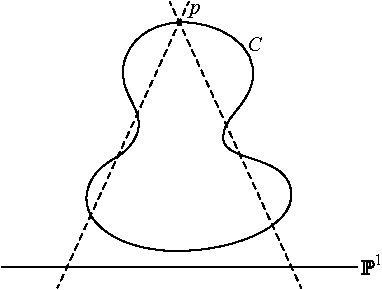
\includegraphics[height=1.7in,trim=0 0 15 0,clip]{main/Fig05-3}%
\llap{\raise12pt\hbox{$\ssty\PP^1$}}
 \caption{Expression of a plane quartic $C$ of genus 3 as a 3-sheeted
\index{3-sheeted cover}%
 cover of $\PP^1$ by projecting the canonical model from a point on it.}
 \label{g13 on quartic}
\end{figure}

There are other representations of $C$ as the normalization of a plane
curve. By
\blue{Clifford's theorem}
\index{Clifford's theorem}%
 $C$ has no $g^2_3$, and the canonical system
is the only $g^2_4$, but there are plenty of models as plane
\blue{quintic curves:}
\index{quintic curve!models}
by Proposition~\ref{very ample}, if $L$ is any invertible sheaf
of degree 5, the linear system $|L|$ will be a basepoint free $g^2_5$
as long as $L$ is not of the form $K+p$, so that $\phi_L$ maps $C$
\blue{birationally}
\index{birationally}%
onto a
\blue{plane quintic curve}
\index{plane quintic curve}%
$C_0 \subset \PP^2` `$. These can
also be described geometrically in terms of the canonical model: any
such invertible sheaf $L$ is of the form $2K-p-q-r$ for some trio of
points $p, q, r \in C$ that are not collinear in the
\blue{canonical model,}
\index{canonical model}%
and we see  that $C_0$ is obtained from the canonical model of $C$ by
applying a
\blue{Cremona transform}
\index{Cremona transform}%
with respect to the points $p, q$ and $r$,
that is, by applying the birational transformation
of the plane defined by the linear series of conics through $p,q,r$.

Proposition~\ref{very ample} implies that a divisor $D$ of degree 6 is
very ample if and only if it is not of the form $K+p+q$ for any $p, q
\in C$ and since the family of invertible sheaves on $C$ has dimension 3,
we see that a general invertible sheaf of degree 6 is very ample (indeed,
this is a simple case of Theorem~\ref{g+3 theorem}).

If $C\subset \PP^3$ is a curve of genus 3 embedded as a curve of degree
6, then $C$ cannot lie on a singular quadric since by
Example~\ref{Div of quadric} it would
have to be a complete intersection of the quadric with a cubic, and then
such a curve has genus 4. If $C$ lies on a smooth quadric
in class $(a,b)$ then $a$ or $b$ would be 2, so $C$ would be
hyperelliptic, and conversely any curve in class $(2,4)$
is a hyperelliptic curve of genus 3, degree 6.

Thus if $C$ is not hyperelliptic, then $C$ does not lie on a quadric
surface. We have $h^0(\sO_{\PP^3}(3)) = 20$ while, by the Riemann--Roch
formula, $h^0(\sO_C(3)) = 18-3+1= 16$, so $C$ lies on (at least) 4
independent cubics. Each of these cubics must be irreducible, so any
two of them
intersect in a curve of degree 9 containing $C$ and another component
or components $D$ of degree totaling 3. By
\blue{Bertini's theorem}
\index{Bertini's theorem}%
if we choose two \emph{general} cubics containing $C$, then each of the
components of $D$ will be smooth. We shall see in
Theorem~\ref{liaison genus formula-first version}
that the arithmetic genus of $D$ must be 0;
thus $D$ must be a
\blue{twisted cubic}
\index{twisted cubic}%
 curve. The ideal of the twisted cubic
is generated by the $2\times 2$ minors of a matrix of the form
$$
\begin{pmatrix}
 \ell_0& \ell_1&\ell_2\\
 \ell_1& \ell_2&\ell_3\\
\end{pmatrix}
$$
where the $\ell_i$ are linear forms,
and it follows that the two cubics can be written as the two $3\times 3$
minors involving the first two rows of  a matrix of the form
$$
\begin{pmatrix}
\label{hilbert-burch matrix}
 \ell_0& \ell_1&\ell_2\\
 \ell_1& \ell_2&\ell_3\\
\ell_4& \ell_5&\ell_6\\
 \ell_7& \ell_8&\ell_9\\
\end{pmatrix}
$$
where $\ell_4,\dots,\ell_9$ are linear forms as well.
From the
\blue{Hilbert--Burch theorem}
\index{Hilbert--Burch theorem}%
(Corollary~\ref{Hilbert-Burch}) one can
show that the ideal of $C$ is generated by the four $3\times 3$ minors
of this matrix, whose columns generate
the
\blue{syzygies}
\index{syzygy}%
of the ideal of the curve.
\marginpar{should we add a forward reference to the def of syzygy?}

\section{Theta characteristics}

In this section we sketch the algebraic theory of theta characteristics,
\index{theta characteristic}%
starting with the case of curves of genus 3.

Suppose that $C \subset \PP^2$ is a smooth plane curve. A \emph{bitangent}
\index{bitangent}%
to $C$ is a line $L \subset \PP^2$ that is either tangent to $C$ at
two distinct points, or has contact of order $\geq 4$ with $C$ at a
point. Alternatively, we can say that a bitangent  corresponds to an
effective divisor of degree 2 on $C$ such that $2D$ is contained in the
intersection of $C$ with a line $L \subset \PP^2` `$.

A naive dimension count suggests that a smooth plane curve should have
a finite number of bitangents (it's one condition on a line $L \in
\redden{(\PP^2)^*}
$ to be tangent to $C$, so it should be two conditions for
it to be bitangent). Indeed, this is the case; by
\blue{B\'ezout's theorem}
\index{B\'ezout's theorem}%
a
conic or cubic curve cannot have any bitangents, but as we will show in
Section~\ref{plane curve pluecker} every smooth curve of degree $d \geq
4$ has
$$
12\,\mbinom{d+1}{4} - 4d(d-2),
$$
counted with appropriate multiplicities\emdash for example, a line simply
\marginpar{parens $\to$ dash}
tangent to~$C$ at 3 points  counts as three bitangents. Accordingly,
\index{bitangent!plane quartic has 28}%
\index{quartic!28 bitangents}%
a smooth plane quartic has 28 bitangents (see the drawing by Pl\"ucker
in Figure~\ref{fig28bitangents}).

The bitangents to a smooth plane quartic $C$ (a canonical curve of genus
3) have a special significance: since $4 = 2 \times 2$, if $D = p+q$ is
a bitangent, then the divisor $2D$ comprises the complete intersection
of $C$ with a line; in other words, we have a linear equivalence
$$
2D \sim K_C
$$
or equivalently the invertible sheaf $\cO_C(D)$ is a
\blue{square root of the canonical sheaf}
\index{square root!of canonical sheaf}%
\index{canonical sheaf!square root of}%
of $C$. Because of their appearance in the theory of
\index{theta function}%
theta functions,
\blue{Riemann}
\index{Riemann, Georg Friedrich Bernhard}%
named the square roots of the canonical sheaf
\emph{theta characteristics}.

How many such square roots are there? If $\cL$ and $\cM$ are invertible
sheaves with $\cL^2 = \cM^2 = K$, then $\cL$ and $\cM$ differ by an
invertible sheaf of order 2; that~is,
$$
\cM = \cL \otimes \cF, \quad \text{where} \quad \cF \otimes \cF \sim
\cO_C.
$$
In other words, $\cF$ is an invertible sheaf of degree 0 and, having
fixed $\sL$,  the other sheaf, $\cM$, corresponds to a point of order
2 in the
\blue{Picard group}
\index{Picard group}%
$\Pic_0(C)$. Since we've seen that $\Pic_0(C) =
\Jac(C)$ is a complex torus of dimension
\marginpar{put $g=3$ in math mode (and a few other letters passim)}
$g =\nobreak 3$\emdash the quotient of $\CC^3$
by a lattice $\Lambda \cong \ZZ^6$\emdash we see that there are $2^6 = 64$
such invertible sheaves, and thus, given that there is some invertible
sheaf $\cL$ satisfying $\cL^2 \cong K_C$, there are exactly $64 = 2^{2g}$
of them.

The reader will have noticed that the number 64 of theta characteristics
does not agree with the number 28 of bitangents. The reason is
\redden{that}
bitangents correspond to \emph{effective} divisors $D$ with $2D
\sim K$, while a theta characteristic $\cL$ may have $h^0(\cL) = 0$,
that is, may not correspond to an effective divisor.
This situation also occurs in other genera.
What can we say about the dimensions $h^0(\cL)$ of the space of sections
of the theta characteristics on $C$?

 There is a beautiful partial answer to this question, which can be
 deduced from a remarkable fact: the dimension $h^0(\cL)$ of the space
 of sections of a theta characteristic mod 2 is invariant in families.
We will now
sketch the necessary results; see \cite{MumfordPaper} and \cite{JHPaper}
for a full treatment.

 \begin{theorem}
 \label{locally constant sign}
 Let $\cC \to B$ be a family of smooth curves, and $\cL_b$ a family of
 theta characteristics on the curves in this family\emdash in other words, an
 invertible sheaf $\cL$ on $\cC$ such that $(\cL|_{C_b})^2 \cong K_{C_b}$
 for each $b \in B$.
\redden{Let} 
$f : B \to \ZZ/2$
\marginpar{for better line breaks}
\redden{be defined by}
 $$
 f(b) = h^0(\cL|_{C_b}) \;  \; (\mathrm{mod\ } 2).
 $$
Then $f$ is locally constant.
\unif
\end{theorem}

We say that a theta characteristic $\cL$ is \emph{even} or \emph{odd}
\index{theta characteristic!parity}%
according to the parity of $h^0(\cL)$. Given the irreducibility of the
space of smooth irreducible curves of genus $g$ (which we'll discuss
in Chapter~\ref{CurvesModuliChapter}),
Theorem~\ref{locally constant sign}
suggests that all curves of genus $g$ have the same number of
even (equivalently, of odd) theta characteristics, and this is in fact
the case.

\begin{theorem}
\label{number of theta characteristics}
If $C$ is a curve of genus $g$, then of the $2^{2g}$ theta characteristics
\index{theta characteristic!number of --s}
on $C$ there are $2^{g-1}(2^g + 1)$ even theta characteristics and
$2^{g-1}(2^g-1)$ odd theta characteristics.
\unif
\end{theorem}

Using Theorem ~\ref{locally constant sign} and the connectedness of the
moduli space of curves,
Theorem~\ref{number of theta characteristics} is reduced to the case when
$C$ is hyperelliptic. We will
\redden{compute the number of theta characteristics in the hyperelliptic case}
\redden{later in this section (page~\pageref{theta characteristic count}).}

\redden{For}
a nonhyperelliptic curve $C$ of genus 3, the
\marginpar{replacing ``Note that in the case of''}
dimension $h^0(\cL)$ of a theta characteristic $\cL$ cannot be $\geq 2$, so
the odd theta characteristics are exactly the effective theta
characteristics, and  this says
\marginpar{dropped ``exactly'' to avoid repetition}
that there are $2^{g-1}(2^g-1)
= 28$ effective theta characteristics corresponding to the 28 bitangents.
\index{bitangents!to a quartic are 28}%

\begin{proof}[Proof of Theorem~\ref{locally constant sign}]
The proof follows,
\redden{thanks to}
\marginpar{made this into a formal proof because it's long. The change from ``via'' to ``thanks to'' is to allow a line break. If you prefer, we could write ``Sketch of proof'' instead of ``Proof''.}
an ingenious construction of
\blue{Mumford's,}
\index{Mumford, David}%
from a  fact about
\blue{quadratic forms}
\index{quadratic form}%
in an even
number of variables.
To state this, recall that if $Q$ is a  bilinear form on $V$ then an
\emph{isotropic plane} is a subspace $\Lambda \subset V$ such that
\index{isotropic plane}%
$Q(\Lambda, \Lambda) = 0$.

\smallbreak

\begin{fact}
\label{isotropic facts}
Suppose that $V$ is a $2n$-dimensional complex vector space with a
nondegenerate
\blue{bilinear form}
\index{bilinear form}%
$Q$.
\vadjust{\goodbreak}%
 \begin{enumerate}
\item The maximal isotropic subspaces for $Q$ have dimension $n$.
\marginpar{replaced semicolons by periods}

\item The set of maximal isotropic subspaces for $Q$ is a subvariety of
the
\blue{Grassmannian}
\index{Grassmannian}%
$G(n,V)$, of dimension $\tbinom{n}{2}$, that has exactly
two connected components (the
\marginpar{why is rulings in quotation marks?}
\blue{``rulings''}
\index{ruling}%
of $Q$).

\item If $\Lambda, \Lambda' \subset V$ are any two maximal isotropic
subspaces, then
$$
\let\quad\enspace
\null\hskip\leftmargini
\dim(\Lambda \cap \Lambda') \equiv n \text{ (mod 2)} \quad \iff \quad
\Lambda, \Lambda' \text{ \,belong to the same ruling.}
$$
\end{enumerate}

A  proof is given in \cite[pp.~735--740]{Griffiths-Harris1978}.
\marginpar{I moved the commentary about the Cheerful Fact to a Remark after the end of the proof, for continuity. }
\end{fact}

Now suppose that $C$ is a smooth curve of genus $g$, and
\redden{let $\cL$ be}
an invertible sheaf on $C$ with $\cL^2 \cong K_C$\emdash that is, a theta
characteristic. Choose a divisor $D = p_1 + \dots + p_n$ of degree $n>
g-1$ consisting of distinct points, and let $V$ be the $2n$-dimensional
vector space
$$
V \colonequals  H^0( \cL(D) / \cL(-D) ).
$$
From the exact sequence
$$
0\to \cL(-D) \to \cL(D) \to \cL(D)/\cL(-D) \to 0
$$
we see that
the sheaf $ \cL(D) / \cL(-D)$ is supported on $D$, with stalk
isomorphic to $\cO_p/\gm_{C,p}^2$ of dimension 2 at each $p \in D$. We
can define a bilinear form on $V$ by setting
\index{residue}%
$$
Q(\sigma, \tau) \colonequals  \sum_i \Res_{p_i}(\sigma \cdot \tau)
\vspace*{-3pt}
$$
where we use the isomorphism $\cL^2 \cong K_C$ to identify the product
\marginpar{\redden{should $\sigma\tau$ be $\sigma \cdot \tau$ as in the display?}}
$\sigma\tau$ with a rational differential.

We now introduce two isotropic subspaces for $Q$.
\redden{The first is}
$$
\Lambda \colonequals  H^0( \cL / \cL(-D) ),
$$
\redden{which}
is isotropic because the product
\redden{of two of its elements}
corresponds to a regular differential, and so has no residues.
Second, we set
$$
\Lambda' \colonequals  \im\left( H^0(\cL(D)) \to H^0( \cL(D) / \cL(-D) ) \right)
.
\marginparhere{added period}
$$
Since  $H^0(\cL(-D)) = 0$, the map is injective and according to
\redden{the Riemann--Roch theorem we have}
$h^0(\cL(D)) = n$, so this is again an $n$-dimensional
subspace of~$V$; it's isotropic because the sum of the residues of a
global rational differential on $C$ is 0. Finally,
$$
H^0(\cL) \cong \Lambda \cap \Lambda',
$$
and Theorem~\ref{locally constant sign} follows.
\end{proof}

\begin{remark}
The first assertion in
Cheerful Fact \ref{isotropic facts}
is
\marginpar{dropped ``completely''}
elementary: since the map
$\widetilde Q : V \ruto \cong V^*$ associated to the form $Q$ carries
\index{isotropic subspace}%
an isotropic subspace to its annihilator, there can't be an isotropic
plane of dimension $>n$; and similarly if $\Lambda \subset V$ is any
isotropic plane of dimension $<n$ we can include $\Lambda$ in a larger
isotropic plane by adding any vector $v$ with $\overkern20 Q(v,v) = 0$
for the induced bilinear form $\overkern20 Q$ on $\ann(\Lambda)/\Lambda$.

The second and third assertions are less elementary, but the reader may
already have seen the first two nontrivial cases of each:
\end{remark}

\begin{example}
When $n=2$ the form $Q$ corresponds to a smooth quadric surface
\marginpar{replaced \{itemize\} by separate examples}
in $\PP^3` `$, and the lines on this surface correspond to the isotropic
2-planes in $\CC^4` `$. There are two rulings by lines, and lines of
opposite rulings meet in a point, while lines of the same ruling are
\marginpar{can't we just say ``disjoint''?}
either disjoint or equal.
\end{example}
\begin{example}
When $n=3$, the Grassmannian $\GG(1,3)$, in its
\blue{Pl\"ucker embedding,}
\index{Pl\"ucker embedding}%
\index{Grassmannian}%
is a smooth quadric in $\PP^5` `$. The isotropic planes in the two distinct
components are easy to describe: in one component they are the projective
2-plane of lines containing a given point $p \in \PP^3` `$. In the other
component they are  the planes corresponding to the lines contained in a
given plane $H \subset \PP^3` `$. Two of these families of lines either
\marginpar{moved ``either''}
intersect
in a point, or coincide; that is, the linear subspaces either
intersect  in a line or a 3-plane. See Exercise~\ref{G13}.
\end{example}

As for proving Theorem~\ref{number of theta characteristics}, it
\marginpar{\redden{is this an intro to the proof just below or an alternate route?}}
is possible to describe the configurations of odd and even theta
characteristics as subsets of the set $S$ of all theta characteristics,
which as we've seen is a principal
\marginpar{principle $\to$ principal}
homogeneous space for the group
$\Jac(C)_2 \cong (\ZZ/2\ZZ)^{2g}$ of
\blue{points of order 2 on the Jacobian}
\index{Jacobian!points of order 2}%
\cite{JHPaper}.

There is more to say about the configuration of theta characteristics. For
example:
\begin{fact}
 As noted, if we choose any theta characteristic on a curve $C$, we may
 identify the set $S^-$ of odd theta characteristics with a subset of the
 group $\Jac(C)_2$ of points of order 2 on the Jacobian of $C$. We might
 expect that some 4-tuples of these points will add up to 0 in $\Jac(C)$;
 in other words, there should exist some 4-tuples $\cL_1,\dots,\cL_4
 \in S^-$ such that
$$
\cL_1+ \dots +\cL_4 = 2K_C.
$$
What this means in the case of genus $g=3$ is that among the 28 bitangents
\index{bitangents!to a quartic are 28}%
to a smooth plane quartic curve $C$, there are some subsets of 4 whose
eight points of tangency form the intersection of $C$ with a plane
conic. From the more detailed knowledge of the configuration $S^-$
we can say how many. Indeed, the number was first found by Salmon
\index{Salmon, George}%
\marginpar{moved and shortened the cite}
\citeyear{MR0115124};
it is 315.
\end{fact}

\subsection*{Counting theta characteristics (proof of Theorem~\ref{number of theta characteristics})}

One
\marginpar{added ``proof of \dots''}
way to count the number of odd and even theta characteristics on
\label{theta characteristic count} % used for page number
a curve of genus $g$ is  to describe
\redden{them}
explicitly in the case of
a hyperelliptic curve and
\marginpar{dropped ``then''}
use Theorem~\ref{locally constant sign}
to deduce the corresponding statements for any smooth curve of genus~$g$.
The reader
\redden{may wish to}
try a relatively simple case in
Exercise~\ref{theta char on genus 2} before looking at the general
case below.
We start with some preliminary calculations:

\begin{lemma}
\label{summing binomials}
For any positive integer $n$,
we have
\let\binom\mbinom
\begin{gather}
\let\;\relax
\sum_{k=0}^n \binom{2n}{2k} \; = \; \sum_{k=0}^{n-1} \binom{2n}{2k+1}
\; = \; 2^{2n-1}
,\\
\sum_{k=0}^n \binom{4n}{4k} = 2^{4n-2}  + (-1)^n 2^{2n-1},
\quad \sum_{k=0}^{n-1} \binom{4n}{4k+2} = 2^{4n-2} - (-1)^n  2^{2n-1}
,\\
\sum_{k=0}^n \binom{4n+2}{4k+1} = 2^{4n} + (-1)^n 2^{2n},
\quad \sum_{k=0}^{n-1} \binom{4n}{4k+3} = 2^{4n} - (-1)^n  2^{2n}
.
\end{gather}
\end{lemma}

\begin{proof}
\let\binom\mbinom
\redden{Equality (1) is}
elementary; by the binomial theorem, we have
$$
2^{2n} = (1+1)^{2n} = \sum_{l = 0}^{2n}@\binom{2n}{l} \quad \text{and}
\quad 0 = (1-1)^{2n} = \sum_{l = 0}^{2n}@(-1)^l\binom{2n}{l}
,
$$
and taking the sum and the difference of these two equations yields the
\marginpar{dropped ``desired''}
result.

\redden{The equalities in (2) follow}
similarly by applying the binomial theorem to the
expression $(1 + i)^{4n} = (-1)^n2^{2n}$. Equating the real parts, we have
$$
\sum_{k=0}^n \binom{4n}{4k} - \sum_{k=0}^{n-1} \binom{4n}{4k+2} =
(-1)^n2^{2n}
,
$$
while by
\redden{(1)}
we have
$$
\sum_{k=0}^n \binom{4n}{4k} + \sum_{k=0}^{n-1} \binom{4n}{4k+2} =
2^{4n-1}.
$$
Taking the sum and difference of these equations yields the desired
\marginpar{dropped ``two''}
formulas.

\redden{For (3)}
we apply the binomial theorem to the expression $(1 + i)^{4n+2} =
 (-1)^n2^{2n+1}i$. Equating the imaginary parts, this gives
\let\;\relax
$$
\sum_{k=0}^n \binom{4n+2}{4k+1} - \sum_{k=0}^{n-1} \binom{4n+2}{4k+3}
\; = \; (-1)^n2^{2n+1}
,
$$
whereas by
\redden{(1),}
$$
\sum_{k=0}^n \binom{4n+2}{4k+1} + \sum_{k=0}^{n-1} \binom{4n+2}{4k+3}
\; = \; (-1)^n 2^{4n+1}
,
$$
and as before taking the sum and difference
\marginpar{dropped ``of these two''}
yields the
result.
\end{proof}

We will count the number of theta characteristics on a hyperelliptic
curve in terms of sums of subsets of the ramification points, so we need
to know what linear equivalences exist among sums of these subsets:

\begin{lemma}
\label{ramification point relations}
Let $C$ be the hyperelliptic curve of genus $g$ expressed as a 2-sheeted
cover of $\PP^1$ with ramification points $p_1,\dots,p_{2g+2}$. The
divisor class of
 any half of the ramification points is equal to the divisor class of
 the other half, but there are no
 smaller relations. More precisely,
 let $I_1,I_2$ be subsets of $\{1,\dots 2g+2\}$
and set
$$
D_i = \sum_{j\in I_i} p_j.
$$
The divisors $D_1,D_2$ are linearly equivalent if and only if $I_1 `= I_2$
\marginpar{added missing ``if''}
or they
have the same cardinality $g+1$ and $I_1`\cup I_2 = \{1,\dots, 2g+2\}$.
\end{lemma}

\begin{proof}
The ``if'' part is simply
\marginpar{dropped ``Note that''}
Corollary~\ref{relation on ramification points} above.

For the ``only if'' part, subtracting whatever points $D_1$ and $D_2$
have in common we may suppose
that $I_1`\cap I_2 = \emptyset$. If $D_1\sim D_2$, it follows at once that
they have the same degree, $d\leq g+1$, and we must show that either $d=0$
or $d=g+1$.

We have $D_1\sim D_2$
\redden{if and only if}
$D_1+D_2\equiv 2D_1$. If
$d\leq g$ we have $r(2D_1) = d$: for $d<g$ this is
the extremal case of
\blue{Clifford's theorem,}
\index{Clifford's theorem}%
while for $d = g$ this follows
simply from the
\blue{Riemann--Roch formula.}
\index{Riemann--Roch formula}%
Thus in case $d \leq g$ every divisor in $|2D_1|$
is a sum of $d$ fibers of the
2 to 1 map of $C$ to $\PP^1` `$, and for such a divisor to be a sum of
distinct points $p_i$
the degree $d$ must be 0, concluding the argument.
\end{proof}

Returning
\redden{now}
\marginpar{filler}%
to the counting, let $C$ be the hyperelliptic curve of genus
$g$, \null
expressed as a 2-sheeted cover of $\PP^1` `$, with ramification points
$p_1,\dots,p_{2g+2}$.

First of all, if we denote the class of the unique $g^1_2$ on $C$ by
$E$, and $D$ is any theta characteristic, then $D+E$ will be effective,
and so we can write
$$
D \sim mE + F
$$
with $-1 \leq m \leq (g@{-}@1)/2$ and $F$ the sum of $g-1-2m$ distinct
points $p_i$.
\marginpar{dropped ``Moreover,''}
This representation is unique, except
\redden{if}
$m=-1$; in that case, we note that the sum of $g+1$ of the branch
points of $C$ is linearly equivalent to the sum of the other $g+1$ by
Corollary~\ref{relation on ramification points}. Thus the total number of
theta characteristics is a sum of binomial coefficients; if $g$ is odd,
it is
$$
\let\binom\mbinom
\binom{2g+2}{0} + \binom{2g+2}{2} + \binom{2g+2}{4} + \dots +
\binom{2g+2}{g-1} + \frac{1}{2}\binom{2g+2}{g+1}
$$
and similarly if $g$ is even it is
$$
\let\binom\mbinom
\binom{2g+2}{1} + \binom{2g+2}{3} + \binom{2g+2}{5} + \dots +
\binom{2g+2}{g-1} + \frac{1}{2}\binom{2g+2}{g+1}.
$$
In either case, we are adding up every other entry in the $(2g+2)$-nd
row of Pascal's triangle, starting from the left and ending up with one
half of the middle term. This sum is exactly one half of the sum of every
other entry in the whole row; by the first part of
Lemma~\ref{summing binomials}
this
\redden{equals}
\marginpar{``is exactly'' occurs just above}
$\sfrac{1}{4} \cdot 2^{2g+2} = 2^{2g}$.

Finally, we can add up the number of even and odd theta characteristics
separately simply by taking every other term in the sums above;
using
\redden{equalities (2) and (3) in}
Lemma~\ref{summing binomials}
(in case $g$ is odd and even, respectively) we can conclude that $C$
has $2^{g-1}(2^g-1)$ odd theta characteristics and $2^{g-1}(2^g+1)$
even theta characteristics. By Theorem~\ref{locally constant sign} and
\marginpar{removed parentheses}
the connectedness of the space of smooth irreducible curves of genus
$g$, this count then holds for all curves of genus $g$, establishing
Theorem~\ref{number of theta characteristics}.
\qed

\section{Exercises}
 \begin{exercise}
  We have seen that a curve $C$ of genus $g=1$ is expressible as a
  2-sheeted cover of $\PP^1$ branched over four points; that is, as
  the smooth projective curve associated to the affine curve $C^\circ
  \subset \AA^2$ given by $y^2 - 
\smash{\prod_{i=1}^{\smash{\lower1.5pt\hbox{$\ssty4$}}} (x-\lambda_i)}$. 
  Show that
  the closure $\overkern22{C^\circ}$ of $C^\circ \subset \AA^2$ in either
  $\PP^2$ or $\PP^1 \times \PP^1$ consists of the union of $C^\circ$ with
  one additional point, with that point a tacnode of $\overkern22{C^\circ}$
  in either case.

  Hint:
\marginpar{dropped ``Observe that''}
 In either case the complement $\overkern22{C^\circ}
  \setminus C^\circ$ consists of a single point, with two points of $C$
  mapping to it; now use the genus formula in either $\PP^2$ or $\PP^1
  \times \PP^1` `$.
  \end{exercise}

\begin{exercise}
Find the number of 
\blue{3-sheeted covers}
\index{3-sheeted cover}%
$C \to \PP^1$ of genus $g$ with
simple branching except for one point of 
\index{simple branch point}%
\index{branch point!simple}%
\blue{total ramification}
\index{total ramification}%
(that is,
one point with just a single preimage point.)

Hint: Such a cover is specified by giving $2g+2$ transpositions, not
all equal, whose product is a nontrivial 3-cycle, modulo simultaneous
conjugation. We have already worked out the number of such tuples whose
product is the identity; just subtract.
\end{exercise}

\begin{exercise}
Let $C$ be a curve of genus $g$. How many 
\blue{unramified double covers}
of $C$
\index{2-sheeted cover!unramified}%
are there?

Hint: Topologically, such covers are in 1-1 correspondence with
subgroups of index 2 in $\pi_1(C)$; and such a subgroup is necessarily
the preimage of a subgroup of index 2 in the abelianization $H_1(C, \ZZ)
\cong \ZZ^{2g}$.
\end{exercise}

\begin{exercise}
Show that unramified 
\blue{double covers}
\index{2-sheeted cover}%
of a smooth curve $C$ are in one-to-one
correspondence
with invertible sheaves $\sL$ on $C$ such that $\sL^2 \cong \sO_C$,
that is with the 
\blue{2-torsion points}
\index{Jacobian!points of order 2}%
of $\Jac(C)$.

Hint: If $f : X \to C$ is an unramified double cover, consider the direct
image $f_*(\cO_X)$. This is a locally free sheaf of rank 2 on $C$,
on which the group $\ZZ/2$ acts; the $+1$-eigenspace is the structure
sheaf $\cO_C$, and the $-1$-eigenspace is an invertible sheaf $\sL$
on $C$ such that $\sL^2 \cong \sO_C$.
\end{exercise}

\begin{exercise} Let $E$ be a curve of genus 1, and $q_1,\dots,q_b \in
E$. How many double covers $C \to E$ are there branched over the $q_i$?

Hint: By our analysis, to specify such a cover, we have to specify the
monodromy around representative loops generating $H_1(E, \ZZ) \cong
\ZZ^2` `$; thus there are four possibilities.
\end{exercise}

\begin{exercise}
\label{ideal of genus 2 degree 5}
In 
\redden{this}
\marginpar{and moved this remark}
exercise, we ask you to complete the
\redden{earlier}
description
of the ideal of a quintic space curve of
genus 2
\redden{(page~\pageref{genus 2 quintic}), keeping the notation.}

Show that for any pair of lines $L, L'$ of the appropriate ruling of $Q$,
\index{quintic!of genus 2}%
the three polynomials $Q$, $S_L$ and $S_{L'}$ generate the homogeneous
ideal $I(C)$. Find relations among them. Write out the minimal resolution
of $I(C)$.

Hint: Choose any line $M \subset Q$ of the opposite ruling, and look
at the linear forms $H, H'$ on $\PP^3$ vanishing on $L \cup M$ and $L'
\cup M$.
\end{exercise}

\begin{exercise}
% an easy case the reader can do before reading the general treatment.
\label{theta char on genus 2}
 Let $C$ be a curve of genus 2, expressed as a 2-sheeted cover of $\PP^1$
 with ramification points $p_1,\dots,p_6$. In this exercise we will
 count the number of
 even and odd theta characteristics.
The text contains the count for a hyperelliptic curve of any genus;
we offer
the case of genus 2 as a warmup.
 \begin{enumerate}
 \item Show that the theta characteristics on $C$ are either of the
 form $\cL = \cO_C(p_i)$ or of the form $\cL = \cO_C(p_i + p_j - p_k)$
 with $i, j, k$ distinct.
 \item Show that in the first case we have $h^0(\cL) = 1$, and in the
 second case we have $h^0(\cL) = 0$.
 \item Finally, show that there are six of the former kind, and 10 of
 the latter, making $2^4 = 16$ in all.
 \end{enumerate}

 Hint: If $h^0(\cL) = 0$, 
\marginpar{to allow line break}
\redden{we have $h^0(\cL(p_k)) = 1$ for any ramification point $p_k$;}
show that  the unique effective divisor in
 $|\cL(p_k)|$ must be the sum of two ramification points.
 \end{exercise}

\begin{exercise}
\label{nodal quartic}
Let $C$ be a  curve of genus 2 and let $\sL\in \Pic_4(C)$ be an invertible
sheaf of the form $L = K_C(p+q)$ with $p \neq q$ and $p+q \not\sim K_C$
as in~\ref{p+q not g12}. Show that
\begin{enumerate}
\item $h^0(L(-2r))= 1$ for any point $r \in C$, and
\item $h^0(L(-2p-2q)) = 0$.
\end{enumerate}
Deduce from this that the map $\phi_L$ is an immersion, and that the
tangent lines to the two branches of $\phi_L(C)$ at the point $\phi_L(p)
= \phi_L(q)$ are distinct, meaning the point $\phi_L(p) = \phi_L(q)$
is a node of $\phi_L(C)$.

Hint: For the first part (which implies that the map $\phi_L$ is an
immersion), observe that $h^0(LK_C^{-1}) = 1$, meaning $p$ and $q$
are unique. The second part says that the images of the differential
$d\phi_L$ at $p$ and $q$ are distinct.
\end{exercise}

\begin{exercise}
\label{G13}
We can represent any line in $\PP^3$ by 2 points on it, 
\marginpar{dropped ``and''}
using their
coordinates as the two rows of a
$2\times 4$ matrix. The \emph{Pl\"ucker coordinates} of the line are
\index{Pl\"ucker coordinates}%
the six $2\times 2$ minors
$$
\{p_{i,j}\}_{0\leq i<j\leq 3}
$$
of this matrix. They are independent, up to a common scalar multiple,
of the two points chosen, and define the \emph{Pl\"ucker embedding}
\index{Pl\"ucker embedding}%
of the 
\blue{Grassmannian}
\index{Grassmannian}%
$\GG(1,3)$ in $\PP^5` `$.

The minors $p_{i,j}$  satisfy a nonsingular quadratic equation: if we
stack two copies of the $2\times 2$
matrix to produce a $4\times 4$ matrix, its determinant is zero, and
the Laplace expansion of this determinant
is the \emph{Pl\"ucker equation}
\index{Pl\"ucker equation}%
$$
p_{0,1}p_{2,3}-p_{0,2}p_{1,3}+p_{0,3}p_{1,2} = 0.
$$

\begin{enumerate}
\item Show that the quadratic form
$
Q = p_{0,1}p_{2,3}-p_{0,2}p_{1,3}+p_{0,3}p_{1,2}
$
is non\-singular, and deduce that it generates the ideal of $\GG(1,3)$
in $\PP^5` `$.
\item
Write the bilinear form corresponding to $Q$ as the determinant of a
matrix, and deduce that
two points in $\GG(1,3)$ correspond to vectors that pair to 0 if and
only if they correspond to lines that intersect.
\item Deduce that a maximal isotropic plane for $Q$ corresponds either to
the set of lines containing a given point or the set of lines contained
in a given plane; and that two such sets of lines 
\redden{(of the same type)}%
\marginpar{\redden{I think you need the red phrase; consider the lines in $P$ and the lines through some $p\in P$.}}
meet in a single point or coincide.
\end{enumerate}
\end{exercise}

\input footer.tex

%header and footer for separate chapter files

\ifx\whole\undefined
\documentclass[12pt, leqno]{book}
\usepackage{graphicx}
\input style-for-curves.sty
\usepackage{hyperref}
\usepackage{showkeys} %This shows the labels.
%\usepackage{SLAG,msribib,local}
%\usepackage{amsmath,amscd,amsthm,amssymb,amsxtra,latexsym,epsfig,epic,graphics}
%\usepackage[matrix,arrow,curve]{xy}
%\usepackage{graphicx}
%\usepackage{diagrams}
%
%%\usepackage{amsrefs}
%%%%%%%%%%%%%%%%%%%%%%%%%%%%%%%%%%%%%%%%%%
%%\textwidth16cm
%%\textheight20cm
%%\topmargin-2cm
%\oddsidemargin.8cm
%\evensidemargin1cm
%
%%%%%%Definitions
%\input preamble.tex
%\input style-for-curves.sty
%\def\TU{{\bf U}}
%\def\AA{{\mathbb A}}
%\def\BB{{\mathbb B}}
%\def\CC{{\mathbb C}}
%\def\QQ{{\mathbb Q}}
%\def\RR{{\mathbb R}}
%\def\facet{{\bf facet}}
%\def\image{{\rm image}}
%\def\cE{{\cal E}}
%\def\cF{{\cal F}}
%\def\cG{{\cal G}}
%\def\cH{{\cal H}}
%\def\cHom{{{\cal H}om}}
%\def\h{{\rm h}}
% \def\bs{{Boij-S\"oderberg{} }}
%
%\makeatletter
%\def\Ddots{\mathinner{\mkern1mu\raise\p@
%\vbox{\kern7\p@\hbox{.}}\mkern2mu
%\raise4\p@\hbox{.}\mkern2mu\raise7\p@\hbox{.}\mkern1mu}}
%\makeatother

%%
%\pagestyle{myheadings}

%\input style-for-curves.tex
%\documentclass{cambridge7A}
%\usepackage{hatcher_revised} 
%\usepackage{3264}
   
\errorcontextlines=1000
%\usepackage{makeidx}
\let\see\relax
\usepackage{makeidx}
\makeindex
% \index{word} in the doc; \index{variety!algebraic} gives variety, algebraic
% PUT a % after each \index{***}

\overfullrule=5pt
\catcode`\@\active
\def@{\mskip1.5mu} %produce a small space in math with an @

\title{Personalities of Curves}
\author{\copyright David Eisenbud and Joe Harris}
%%\includeonly{%
%0-intro,01-ChowRingDogma,02-FirstExamples,03-Grassmannians,04-GeneralGrassmannians
%,05-VectorBundlesAndChernClasses,06-LinesOnHypersurfaces,07-SingularElementsOfLinearSeries,
%08-ParameterSpaces,
%bib
%}

\date{\today}
%%\date{}
%\title{Curves}
%%{\normalsize ***Preliminary Version***}} 
%\author{David Eisenbud and Joe Harris }
%
%\begin{document}

\begin{document}
\maketitle

\pagenumbering{roman}
\setcounter{page}{5}
%\begin{5}
%\end{5}
\pagenumbering{arabic}
\tableofcontents
\fi


\chapter{Fine moduli spaces}
\label{Moduli chapter}
\label{ModuliChapter}

\section{What is a moduli problem?}

Algebraic geometry is special among geometric theories in
that
the objects involved\emdash varieties,  schemes or maps between
them\emdash can be parametrized by other varieties or schemes. The set
of submanifolds of a given manifold, or more generally of maps between
two given manifolds, seems too large to be given the structure of a
finite-dimensional manifold itself. By contrast, any algebraic variety
is specified by a finite collection of polynomials, which in turn have
a finite number of coefficients, so it's not too far-fetched that the
set of all varieties with specified numerical invariants, or
morphisms between two given varieties, could be given the structure of
a ``moduli space'' that is a variety (or scheme or\dots) in its own
right.

For an example\emdash perhaps the original one\emdash projective plane
curves of degree $d$
are in natural one-to-one correspondence with the forms of degree $d$
modulo the group of nonzero scalars\emdash that is, with the points of
the dual of the projective space
$ \PP(H^0(\sO_{\PP^2}(d)))=\PP^{\sbinom{d+2}{2}-1} $.
Thus, for example, plane cubics are parametrized by $\PP^{9}$, and a
family $\cC \to B$ of cubics corresponds to a map $\phi: B \to \PP^9$ 
(Figure~\ref{cubic family}).
In this chapter, we'll give a general framework for the notion of moduli
space, introducing the main examples that we will treat in this book.

\begin{figure}
\vskip-14pt
$
  \vcenter{\hbox{\includegraphics[width=0.84in,trim=0 27 7 25,clip]{"main/Fig06-1a"}}}\hskip0.6em
  \vcenter{\hbox{\includegraphics[width=0.7in]{"main/Fig06-1b"}}}\quad
  \vcenter{\hbox{\includegraphics[width=0.7in]{"main/Fig06-1c"}}}\quad
  \vcenter{\hbox{\includegraphics[width=0.7in]{"main/Fig06-1d"}}}
$
\vskip-3pt
 \caption{A one-parameter family of plane cubics.}
 \label{cubic family}
\end{figure}

There are several ways in which the possibility of making moduli spaces
has been useful in algebraic geometry. First, the existence of a moduli
space that  parametrizes objects of a certain type allows us to speak
of the ``general \null object,'' meaning that we allow ourselves to avoid the
 properties of ``special objects'' parametrized by closed subvarieties
of the moduli space. For example, we can make precise sense of the
statement ``The general plane curve of degree $d$ is smooth.'' It means 
that the set of smooth curves corresponds to an open subset of the projective space $\PP^{\sbinom{d+2}{2}-1} $.
 We have already used this
possibility in many places in this book.

Second, it allows us to speak coherently about
families of objects. Some moduli spaces carry \emph{universal families},
\index{universal family}%
and every nice family of the sort of objects
they parametrize is pulled back from this one by a unique map.

This idea was already exploited informally in the nineteenth century in
\index{historical context}%
\index{preservation of number}%
the guise of ``preservation of number,'' used to count configurations of
points or curves with a given property by specializing the
data, and we have also exploited this idea in
Chapter~\ref{JacobianChapter} to explain the count of odd and even
theta characteristics on a general curve by appealing to the existence
of a specialization to a hyperelliptic curve. In a related manner, we
have already seen how the fact that invertible sheaves of degree $d$
on a curve $C$ are parametrized by a $g$-dimensional variety allows us
to prove the $g+3$ theorem (Theorem~\ref{g+3 theorem}).

Third, to the extent that we can describe the intersection theory of a
moduli space, it opens up the possibility of doing
enumerative geometry
\index{enumerative geometry}%
on it to count solutions of geometric problems\emdash and in particular
to prove the existence of solutions. For example, knowing that the
\index{P@$\PP^3$!any 4 curves intersect a common line}%
parameter space for lines in $\PP^3$ is the Grassmannian $\GG(1,3)$,
\index{Grassmannian $\GG(1,3)$}%
a projective variety of dimension 4, and that the condition that the
set of lines meeting a given curve of degree $d$
is a divisor linearly equivalent to  $d$ times the hyperplane section
(Figure~\ref{Chow degree}), we can conclude  that there exists a line
in $\PP^3$ meeting any four given curves \cite[Section 3.4.1]{3264}. We
will use the same idea to prove the much deeper existence of certain
linear series on all curves (the existence half of the Brill--Noether
theorem, discussed in Chapter~\ref{Brill--Noether}).

\begin{figure}
\centerline {\includegraphics[height=1.4in]{"main/Fig06-2"}}
 \caption{A general  one-parameter linear family of lines in $\PP^3$\emdash that is, the family of lines
 contained in a general plane and passing through a general point in that plane\emdash meets a space curve $C$ in
 $\deg C$ points.}
 \label{Chow degree}
\end{figure}

In modern terms, a \emph{moduli problem}
\index{moduli problem}%
consists of a class of objects
in algebraic geometry\emdash schemes, subschemes of a given scheme,
maps of schemes,
sheaves on schemes, typically defined by some common
attributes\emdash and a notion of what it means to have a \emph{family}
\index{family}%
of these objects parametrized by a scheme $B$. The notion is formalized
in the idea of a \emph{moduli functor},
\index{moduli functor}%
which associates to each scheme $B$ the set of families over $B$ of the
given sort. Examples will make this vague notion more concrete.

%\subsection*{Some moduli problems}

%\begin{enumerate}
%\label{list of moduli problems}

\begin{example}[effective divisors on a given curve] The objects are
\index{moduli functor}%
\index{effective divisor!family of --s on a curve}%
effective divisors of given degree on a given smooth, projective curve
$C$. A family of such divisors is a subscheme $\cD \subset B \times C$,
flat of degree $d$ over $B$.
Here we are using
the equivalence between divisors of degree $d$ on a smooth curve and
degree $d$ subschemes of the curve. The moduli space is the $d$-th
symmetric power
\index{symmetric power}%
$C_d$ of $C$, discussed in Section~\ref{symmetric section}.
\end{example}

\begin{example}[invertible sheaves on a given curve] The objects are
\index{invertible sheaves!family of --s on a curve}%
invertible sheaves on a given smooth projective curve $C$. A family
over a scheme $B$ is an equivalence class of invertible sheaves $\cL$
on $B \times C$ whose restriction to each fiber of $B \times C$ over
$B$ has degree $d$, where two families $\cL$ and $\cL'$ on $B \times
C$ are equivalent if $\cL\cong \cL' \otimes \cM$, where $\cM$ is  an
invertible sheaf pulled back from $B$. Usually one restricts attention
to invertible sheaves
whose restrictions to each fiber $b\times C$ have a given degree $d$.
\index{Jacobian}%
\index{Picard variety}%
The moduli spaces are the Jacobian and Picard varieties,
discussed in
Section~\ref{Picard section}.
\end{example}

\begin{example}[moduli of smooth curves] The objects are isomorphism
\index{smooth curve!moduli of --s}%
classes of smooth, projective curves of genus $g$. A family over $B$
is an equivalence class of smooth, projective morphisms $f : \cC \to B$
whose fibers are curves of genus $g$, where two such families $f, f'$
are equivalent if there is an isomorphism from the source of $f$ to
the source
of $f'$ making the
following diagram commute:
$$
\begin{diagram}[small]
\cC && \rTo^\cong && \cC'\\
&\rdTo_f&&\ldTo_{f'}\\
&&B
\end{diagram}
\vspace*{3pt}
$$
The moduli spaces $M_g$ of curves are harder to construct, and we will
have a separate discussion of them in
Chapter~\ref{CurvesModuliChapter}. Nonetheless,
it will be useful at several points in this chapter to assume their
existence.
\end{example}

\begin{example}[Hurwitz spaces] An object is a smooth projective curve $C$
\index{Hurwitz space}%
of a given genus, together with a map $f: C\to \PP^1$ of given degree, up
to isomorphisms of the curves that commute with the map, as in this diagram:
$$
\begin{diagram}[small]
C && \rTo^{\cong} && C'\\
&\rdTo_f&&\ldTo_{f'}\\
&&\PP^{1}
\end{diagram}
$$
A family over $B$ is a family $\cC \to B$ of smooth projective curves
of a given genus, together with flat map $\cC \to B\times \PP^{1}$
of degree $d$.
 Often the allowable ramification indices are specified. We will discuss
 the simplest Hurwitz scheme in Chapter~\ref{CurvesModuliChapter}.
\end{example}

\begin{example}[Severi varieties] The objects are plane curves
\index{Severi variety}%
\label{Severi}%
of given degree $d$ and geometric genus $g$. If $g \neq \tbinom{d-1}{ 2}$
the curves will necessarily be singular, but are often
constrained to have only mild singularities, usually only nodes. We will
discuss
Severi varieties
in Chapter~\ref{CurvesModuliChapter}.
\end{example}

\begin{example}[Hilbert schemes] The objects are subschemes of a given
\index{Hilbert scheme}%
projective space;   a family over $B$ is a subscheme $\cC \subset B \times
\PP^r` `$, flat over $B$. Since the Hilbert polynomials of the fibers
of a
flat family
\index{flat family}%
are all equal
\cite[Chapter III, \S9]{Hartshorne1977},
the Hilbert scheme is the disjoint union of subschemes corresponding to
particular Hilbert polynomials, and these subschemes are of finite type.
\index{finite type}%
If $B$ is reduced then the flatness condition is equivalent to the
constancy of the Hilbert polynomial (\cite[Theorem 9.9]{Hartshorne1977} or \cite[Chapter III, \S 3.2]{DE-JH-schemes}).

In Chapter~\ref{HilbertSchemesChapter} we
study the
open set consisting of smooth curves $C\subset \PP^{r}$ of given degree
and genus.
\end{example}

\section{What is a solution to a moduli problem?}

Typically what we want from a solution to a
moduli problem
\index{moduli problem}%
is to
understand all possible families of the objects
in question. In particular, the individual objects should be in natural
\index{natural correspondence}%
one-to-one correspondence with the closed points of the
moduli space.  The word \emph{natural} is the key. Most of the time,
the set of objects we are interested in has
the cardinality of the continuum,
as do all positive-dimensional varieties $M$ over $\CC$, so a mere
bijection between the points of $M$ and the objects to be parametrized
is meaningless.

In the nicest situations there is a
\emph{universal} family
\index{universal family}%
$\phi:
\cX\to M$ of these objects over $M$,
such that any family over a scheme $B$  is pulled back from the one on
$M$ via a unique morphism $B\to M.$  Such a space $M$ with its universal
family $\phi$, if it exists, is called a \emph{fine moduli space}. This
\index{fine moduli space}%
\index{moduli space!fine}%
can be expressed more abstractly but more succinctly by saying that the
moduli scheme \emph{represents the moduli functor}, which means there
is an isomorphism of functors
$$
\{ B \mapsto \text{families of } X \text{ over } B \} \cong \{ B\mapsto
\mathrm{{Mor}}_{\mathrm{ Schemes}}(B, M) \}.
$$
If $M$ is a fine moduli space then the identity map $M\to M$ corresponds
to the ``universal family'' $\phi: \cX \to M$.
The Hilbert scheme, as well as $\Div_d(C)$ and $\Pic_d(C)$ are fine moduli
spaces but the moduli space of curves
and the Hurwitz schemes are not.

If a fine moduli space and its universal family exist, then it is unique
up to unique isomorphism: given two avatars $M$ and $M'$
the universal family on $M$ corresponds to a map $M\to M'$, and we
similarly produce a map $M'\to M$. The pullback of the universal family
on $M$ by the composition of these two maps is again the universal family,
so the composition is the identity map.

Although the moduli space of curves and the Hurwitz spaces are not fine
moduli spaces, they are still defined
in a way that makes them unique, as we shall see below.

\def\eps{{\epsilon}}
One of the useful features of a fine moduli space is that it makes the
computation of tangent spaces relatively easy.
\index{tangent space}%
\index{Zariski tangent space}%
Recall that if $(R,\gm)$ is the local ring at a point $m$ on a variety
$\cM$ then the (Zariski) tangent
space to $M$ at $m$ is the vector space of linear functionals
$\Hom_{R/\gm}(\gm/\gm^2, R/\gm)$.   Assuming that
$R$ contains its residue field $k \colonequals  R/\gm$, such functionals
are precisely the restrictions to $\gm/\gm^2$ of the ring homomorphisms
$R \to k[\eps]/(\eps^2)$ inducing the identity on $k$.
 If $\cM$ is a fine moduli space for some functor $F$, then such maps
 are in one-to-one correspondence
with the set $F(E)$ of families over $E \colonequals
\Spec(k[\eps]/(\eps^2))$.

The vector space structure on the tangent space is also accessible from
this description:  the
 sum of tangent vectors corresponding to families $X_i \to E$ is the
 restriction to the diagonal
 $E \subset E\times E$
 of the product family $X_1 \times X_2 \to E\times E$.
Often one can to compute the tangent space to a moduli space before even
knowing that the moduli space exists!

\section{Hilbert schemes}
\label{hilbert scheme section}

The Hilbert scheme is a fine moduli space representing the functor of
\index{flat family!of subschemes}%
\index{subscheme!family of --s}%
\index{Hilbert scheme|(}%
flat families of subschemes of $\PP^r` `$,
that is, the functor that takes a scheme $B$ over $\CC$ to the set of
subschemes $\sX \subset B\times \PP^r$
that are flat over $B$; a morphism $f: B'\to B$ induces a map carrying
a family to the pullback of the family by $f$.

\begin{example}[the Hilbert scheme of plane curves]
\label{Hilb for plane curves}
Let $p(m) \colonequals  dm+1-\tbinom{d-1}{ 2}$ be the Hilbert polynomial of
a
plane curve
\index{plane curve}%
of degree $d$, and consider the family
$\Hilb_{p(m)}(\PP^2)$
\index{notation!$\Hilb_{p(m)}$}%
of schemes $X \subset \PP^{2}$ having Hilbert polynomial $p$. Since
$\dim X = \deg p = 1$, $X$ has at least one component that is
1-dimensional. The union of such components must have degree
equal to $d$, the leading coefficient of $p(m)$. Since the Hilbert
polynomial  of this union is also equal
to $p(m)$ we see that $X$ is in fact a (possibly nonreduced and/or
reducible) plane curve of degree $d$. The space $\Hilb_{p(m)}(\PP^2)$
is the projective space $\PP^{\sbinom{d+2}{2}-1}$ of forms of degree $d$,
and the universal family is the projection
universal family
\index{universal family}%
$$
\bigl\{@(x,F) \in \PP^2 \times \PP^{\sbinom{d+2}{2}-1} \mid F(x)=0@\bigr\} \to
\PP^{\sbinom{d+2}{2}-1}.
$$

More typically, the set of curves $C \subset \PP^r$ of degree $d$ and
genus $g$ corresponds to a subset of the Hilbert scheme parametrizing
subschemes of $\PP^r$ with Hilbert polynomial $p(m) = dm - g + 1$, though
not all schemes with this Hilbert polynomial are purely one-dimensional
subschemes, as we shall see.
\end{example}

In this section
we
compute
the Zariski tangent space to the Hilbert scheme at a point and
\index{Zariski tangent space}%
\index{Hilbert scheme!at a point}%
sketch the construction of the scheme itself. For a rigorous
treatment including many generalizations,  see \cite{HomogHilbert}
or \cite{MR2222646}. In Chapter~\ref{HilbertSchemesChapter}, we'll
describe  the
open subsets of smooth curves in the Hilbert schemes of curves of low
degree and genus in $\PP^3$ in more detail.

\subsection[The tangent space to the Hilbert scheme]{\hskip-3pt The tangent space to the Hilbert scheme}
%\label{tan hilbert section}

Following the general recipe for tangent spaces to fine moduli spaces,
we need to understand
flat families
\index{flat family}%
of projective schemes over $E \colonequals  \Spec
\CC[\eps]/(\eps^2)$. Recall
from
\cite[p.\,182]{Hartshorne1977},
for example,
that if
$X\subset \PP^r$ is a smooth subscheme then
 the normal bundle $\sN_{X/\PP^r}$ of $X$ in $\PP^r$ is defined in terms
 of the tangent bundles
 of $X$ and $\PP^r$ by the exact sequence:
$$
0\to \sT_X \ruto {\phi} \sT_{\PP^r}|_X \to \sN_{X/\PP^r} \to 0.
$$
Thus a global section of
$\sN_{X/\PP^r}$
\index{infinitesimal motion of a curve}%
can be thought of as an infinitesimal motion of~$X$ (Figure~\ref{perturbed
curve}).

\begin{figure}
\centerline {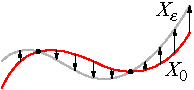
\includegraphics[width=1.35in]{main/Fig06-0-new}}
\vskip-5pt
 \caption{Infinitesimal perturbation of a curve by a normal vector field.}
 \label{perturbed curve}
\end{figure}

To define the normal sheaf for locally complete intersection subschemes
$X$ we first define the
\emph{conormal sheaf}
\index{conormal sheaf}%
to be the kernel of the dual  of $\phi$, which is the natural map
$\Omega_{\PP^r}|_X \to \Omega_X$,
and since $X$ is locally a complete intersection, this corresponds to
the exact sequence:
$$
0\to \sI_{X/\PP^r}/\sI_{X/\PP^r}^2 \to \Omega_{\PP^r}|_X \to \Omega_X
\to 0.
$$
We thus define $\sN_{X/\PP^r} \colonequals
\sHom(\sI_{X/\PP^r}/\sI_{X/\PP^r}^2, \sO_X)$.

By analogy we define the
\emph{normal sheaf} of any subscheme $X\subset
\index{normal sheaf}%
\PP^r$
$$
\sN_{X/\PP^r} \colonequals  \sHom(\sI_{X/\PP^r}/\sI_{X/\PP^r}^2, \sO_X).
$$
The following theorem shows that this
has the same connection with infinitesimal motions for arbitrary
subschemes $X$.

\begin{theorem}
\label{tangent space of Hilb}
Let $X\subset \PP^r$ be a subscheme with Hilbert polynomial $p(m)$ and let
$E = \Spec\CC[\eps]/(\eps)^{2}$. The flat families
$\sX \subset \PP^r\times E$ specializing to $X$ at the closed point
defined by $(\eps)$
are in natural one-to-one correspondence with the vector space
\index{Zariski tangent space!to the Hilbert scheme}%
$\Hom_{\PP^r}(\sI_{X/\PP^r}, \sO_X) = H^0(\sN_{X/\PP^r})$, which is thus
the tangent space to the Hilbert scheme $\Hilb_{p}(\PP^r)$ at $[X]$.
\end{theorem}

\begin{proof}
We will actually treat the analogous result for an affine subscheme $X
\subset \AA^r = \Spec S$, where
$S = \CC[x_{1}, \dots, x_{r}]$; since our construction is natural,
it will patch on an affine cover to give the projective case stated above.

An $E$-module $M$ is flat
\index{flat module}%
over $E$ if and only if $\Tor_1^E(\CC,M) = 0$.
Since the
free resolution
\index{free resolution}%
of $\CC$ as an $E$-module has the form
$$
\cdots \ruto {\ \eps} E \ruto {\ \eps} E \ruto {\ \eps} E
\ruto{}\ \ \CC \ruto{}\ \ 0,
$$
we have $\Tor_1^E(\CC,M)=0$ if and only if the submodule of $M$
annihilated by $\eps$ is $\eps M$.

We first construct a flat family from a homomorphism: Let
$$I = (g_1,\dots,
g_t)\subset S = \CC[x_1,\dots, x_r]
$$
be the ideal defining $X$.
Note that $\Hom_S(I/I^2, S/I) = \Hom_S(I,S/I)$. Let $\phi: I\to S/I$
be a homomorphism, and let $h_i\in S$ be
any element reducing to $\phi(g_i)$ modulo $I$.  The ideal
$$
I' \coloneqq  (g_1+\eps h_1,\dots, g_t+\eps h_t)\subset
S[\eps]/(\eps^2) \equalscolon S'
$$
defines a scheme $\Spec S'`/@I'$  over $E$ which restricts to $X$ modulo
$(\eps)$; that is, $I' +\nobreak (\eps) =\nobreak  I$.

To see that $I'$ is
independent of the lifting chosen,
consider
$k_1,\dots,k_t\in I$
such
that the elements $g_i+\eps(h_i+k_i)$ are a different lifting,
generating an ideal~$I''$.
Writing $k_i = \sum r_{i,j}g_j$ we have
$$
g_i+\eps(h_i+k_i) = g_i+\eps h_i+ \sum \eps r_{i,j}(g_j+\eps h_j)
,
$$
 so
$I'' \subset I'$, and symmetrically $I' \subset I''$.

To prove flatness, suppose that $a\in S'$ and  $\eps a  \in I'$,
so that we can write  $\eps a= \sum(r_i+\eps s_i)(g_i+\eps h_i)$ for
some $r_{i}, s_{i} \in S$.
It follows that
$\sum r_i\g_i = 0$. Since $\phi$ is a homomorphism this implies $\sum
r_i h_i \in I$. Thus
$\eps a \in  \eps I\subset S'$, whence $a\in I + (\eps)$.  Writing $a
=\sum p_i g_i+\eps b'$
and using the relations $g_i \equiv -\eps h_i \hbox{ mod } I'$ we get
 $a \equiv \eps (-\sum p_i h_i+b') \hbox{ mod } I'$, as required.

Finally, starting from a flat family $S'`/@I'$ over $E$ with $I' + (\eps)
= I +\eps$,
let $J$ be the image of $I'$ in $S'/(\eps I) = S \oplus (\eps S)/(\eps
I)$. We claim that $J$ is the graph of a homomorphism $\phi: I \to
(\eps S)/(\eps I) \cong S/I$.

Since $I' + \eps S = I +\eps S$,  the projection  to the  summand
$S\subset S'$ maps $J$ onto~$I$.
To prove that $J$ is the graph of a homomorphism, it suffices to show
that this projection is an isomorphism.
The kernel is
the intersection of $J$ with $(\eps S)/(\eps I )$, so we must show that
if $r\in S$ and $\eps r \in I'$ then $\eps r \in \eps I$.

Since $\eps r \in I'$, the condition of flatness implies
that the image of $r$ in $S'`/@I'$ is in $\eps(S'`/@I')$, which is to say
that $r \in I' + \eps S = I +\eps S$.
Thus $r \in  I + \eps S,$ whence $\eps  r \in \eps I$ as required.

This shows that
$J$ is the graph of a homomorphism $\phi$ such that
 $I'$ is generated by $\{g+\phi g\mid g\in I\}$, so the two constructions
 are inverse to
each other.
\end{proof}

\begin{example}
\label{Hilb for plane curves-continued}
If $C$ is the
plane curve
\index{plane curve!Hilbert scheme}%
of degree $d$ defined by a form $F$, then the
ideal sheaf of $C$ is $\sO_{\PP^2}(-d)$, and thus
$$
\sHom(\sI_{C/\PP^2}/\sI_{C/\PP^2}^2, \sO_{C}) = \sO_{\PP^2}(d)|_C =
\sO_C(d).
$$
From the exact sequence
$$
0\to\sO_{\PP^2}\ruto {\,F}\sO_{\PP^2}(d) \to\sO_C(d)\to 0
$$
we deduce that the dimension of the tangent space to
$\Hilb_{p(m)}(\PP^2)=\PP^{\sbinom{d+2}{2}-1}$  at $C$
with $p(m) = dm+1-\tbinom{d-1}{ 2}$,
is $h^0(\sO_C(d)) = h^0(\sO_{\PP^2}(d))-1 = \dim \PP^{\sbinom{d+2}{2}-1}$,
as expected.
\meshing
\end{example}

\subsection{Parametrizing twisted cubics}

By Lemma~\ref{smooth is open}
below, the set of twisted cubics\emdash that is, smooth, irreducible,
nondegenerate curves of degree 3 in $\PP^3$\emdash is an open subset
of the Hilbert scheme $\Hilb_{3m+1}(\PP^3)$. As we've seen, a twisted
\index{twisted cubic}%
cubic curve $C \subset \PP^3$ can be described as the zero locus of
three homogeneous quadratic polynomials $Q_1, Q_2$ and $Q_3$ in the
homogeneous coordinates on $\PP^3$; to specify the twisted cubic
we could just list the $3 \times 10 = 30$ coefficients of these. But
of course we could replace the three quadrics $Q_i$ with any three
independent linear combinations of them; what matters\emdash and what
is naturally associated to $C$\emdash is the vector space $V = \langle
Q_1, Q_2, Q_3 \rangle \subset H^0(\cO_{\PP^3}(2))$. This suggests that
we consider the map of sets
$$
h : \{ \text{twisted cubic curves } C \subset \PP^3 \} \to G = G(3,
H^0(\cO_{\PP^3}(2)))
$$
obtained by associating to a twisted cubic $C$ the second graded piece
of its homogeneous ideal.

This differs significantly from
the example of plane curves introduced in the second paragraph of this chapter (page~\pageref{ModuliChapter}; see also Examples \ref{Hilb for plane curves} and \ref{Hilb for plane curves-continued}):
there, the objects to be parametrized were the
zero locus of a single polynomial, and we could vary those coefficients
arbitrarily and still have a plane curve; thus, the image of the analogous
map was open in the projective space $\PP^{\sbinom{d+2}{2}-1}$. But if
we generically
perturb the coefficients of the three quadratic polynomials $Q_i$
defining the twisted cubic the resulting quadrics will
be a complete intersection, generating
 the ideal of a set of eight points. Thus the image of the map $h$
 does not contain an open set of $G$.
We will give equations defining the image in Section~\ref{hilb
construction}, and we can consider it
the Hilbert scheme of twisted cubics.

As in this case, we will mainly be   interested in the subsets of the
Hilbert schemes corresponding to smooth irreducible curves:

\begin{lemma}
\label{smooth is open}
Suppose that $X \to B$ is a flat family of projective schemes (that is,
\index{flat family of projective schemes}%
the projection to the second factor of
$X\subset B\times \PP^n$  is flat). The points $b\in B$ such that the
fiber $X_b$ is smooth and irreducible form an open set.
\end{lemma}

\begin{proof}
To prove the
lemma we may assume that $B = \Spec A$ is affine and
irreducible. Let $x_{0}\dots, x_{r}$ be homogeneous coordinates
on $\PP^{r}$, and suppose that
$X\subset \PP^{r}_{\CC}$ is defined by the ideal $I_{X} = (F_{1}, \dots,
F_{n}) \in A[x_{0}, \dots x_{r}]$.
Since $X$ is flat over $B$ the fiber dimension $d$ is constant, and the
singular locus
of a given fiber $X_{b}$ is  the subscheme of $X_{b}$ defined by the
ideal $J$ of
$(r-d)\times (r-d)$ minors of the Jacobian matrix $(\partial
F_{i}/\partial x_{j})$.

Let $Y\subset B\times \PP^{r}$ be the closed subscheme defined by $J$
alone.
It follows that $Y\cap X \subset X$ defines a scheme of singular points
of fibers of the family, so this set is closed
in $X$.
Since the map $X \to B$ is projective, the image of $X\cap Y$ is closed,
and its complement is open.
 Finally, a smooth fiber $X_b$ is irreducible if and only~if it is
 connected. This holds if and only if $h^0(\sO_{X_b}) <2$ and by the
base change theorem
\index{base change theorem}%
\cite[Theorem 12.11]{Hartshorne1977} this set
 is open as well.
\end{proof}

\begin{proposition}
\label{hilb of twisted cubics}
The open subset $\cH^\circ$ of the Hilbert scheme $\Hilb_{3m+1}(\PP^3)$
para\-metrizing twisted cubics is irreducible of dimension $12$.
\unif
\end{proposition}

\begin{proof}
Let $C_0 \subset \PP^3$ be a twisted cubic, and consider the family
\index{PGL@$\PGL_4$}%
of translates of $C_0$ by automorphisms $A \in
\PGL_4
$ of $\PP^3$:
that is, the family
$$
\cC = \bigl\{@(A, p) \in \PGL_4 \times \PP^3 \; \mid \; p \in A(C_0)@\bigr\}.
$$
Via the projection $\pi : \cC \to \PGL_4$, this is a family of twisted
cubics, and so it induces a map
$$
\phi : \PGL_4 \to \cH^\circ.
$$
Since every twisted cubic is a translate of $C_0$, this is surjective,
with fibers isomorphic to the stabilizer of $C_0$, that is, the subgroup
of $\PGL_4$ of automorphisms of $\PP^3$ carrying $C_0$ to itself. By
Exercise~\ref{projective automorphism}, every automorphism of $C_{0}$ is
induced by an automorphism of $\PP^{3}$, so the stabilizer is isomorphic
to $\PGL_2$ and  thus has dimension 3. Since $\PGL_4$ is irreducible of
dimension 15, we conclude that $\cH^\circ$ is irreducible of dimension 12.
\end{proof}

\subsection{Construction of the Hilbert scheme in general}
\label{hilb construction}

The Hilbert scheme is more complicated than would appear from the examples
above, and this is even true
for the Hilbert polynomial $3m+1$. There are many subschemes of $\PP^3$
that have the same Hilbert polynomial $3m+1$ as a twisted cubic\emdash
for example, the union of a plane cubic and a point\emdash and are
not the intersection of the quadrics containing them. (See Exercises
\ref{characterization of degree} and~\ref{deg of disjoint union}.) In
Chapter~\ref{HilbertSchemesChapter} we will discuss many more components
of Hilbert schemes.

A fundamental result of
\index{Matsusaka, Teruhisa}%
Matsusaka provides a place to start:

\begin{npt}
\begin{theorem}[\cite{Matsusaka}]
\label{matsusaka}
Let $p(m) \in \QQ[m]$ be a polynomial. There exists an integer $m_0$
\index{Matsusaka's theorem}%
such that:

\begin{enumerate}
\item For any subscheme $X \subset \PP^r$ with Hilbert polynomial
$p_X = p$ we have
$$
h^0(\cI_{X/\PP^r}(m)) = \mbinom{m+r}{r} - p(m) \quad \text{for all }
m \geq m_0;
$$
in other words, the Hilbert function of $X$ agrees with the Hilbert
polynomial $p_X = p$ for all $m \geq m_0$.

\item For any subscheme $X \subset \PP^r$ with Hilbert polynomial $p_X =
p$ and
the saturated ideal of $X$ is defined by forms of degree $\leq m$.
\end{enumerate}
\end{theorem}
\end{npt}

Note that for any given $X$ the existence of an $m_0$ satisfying the
\index{Serre--Grothendieck vanishing theorem}%
statement of the lemma is immediate by
Theorem~\ref{Serre--Grothendieck vanishing}. The point of the lemma is
that we can find one value of $m_0$ that works for all $X$ with
Hilbert polynomial $p$. The following result of Gotzmann~\citeyear{Gotzmann}
provides a method for determining $m_0$.

\begin{theorem}
The Hilbert polynomial  of the homogeneous coordinate ring of any scheme
$X\subset \PP^r$ can be written uniquely in the form
$$
\chi(\sO_X(m)) = \mbinom{m+a_1}{a_1}+ \mbinom{m+a_2 -1}{a_2}+ \cdots+\mbinom{m+a_s -(s-1)}{a_s}
$$
with
$$
a_1\geq \cdots \geq a_s \geq 0,
$$
where the binomial coefficients are interpreted as polynomials in
$m$. Moreover, the saturated homogeneous ideal of $X$ is
 generated in degrees $\leq s$, and one can take $m_0 = s$ in the
 construction of the Hilbert scheme above.
\unif
\end{theorem}

See \cite{MR1023391} %Green-Gotzmann
for an exposition and a proof. From the coefficients $a_j$ one can read
off uniform vanishing theorems for $H^i(\sI_X(m))$
 as well.

 For example, the Hilbert polynomial $3m+1$ of the twisted cubic may be
 written as
 $$
 3m+1 =  \mbinom{m+1}{1}+ \mbinom{m+1 -1}{1}+\mbinom{m+1 -2}{1}+
\mbinom{m+0 -3}{0},
 $$
 Here $s=4$, and indeed the homogeneous ideal of the union of a plane
 cubic with a point, also in the plane,
 requires equations of degree 4.

\subsection{Grassmannians}
\label{Grassmannian section}

The
simplest and most fundamental
Hilbert schemes are the
Grassmannians\emdash including the projective spaces themselves.
\index{Grassmannian}%
They
\null
parametrize the families of linear subspaces of given dimension in
vector spaces or in projective spaces.
For $0\leq k\leq r$ we write $\GG(k,r)$ for the set of $k$-planes in
\index{notation!$\GG(k,r)$}%
$\PP^{r}$ and identify it with
$G(k+1,r+1)$, the set of $(k+1)$-dimensional vector subspaces of an
$(r+1)$-dimensional vector space.
When we want to make the $(r+1)$-dimensional vector space $V$ explicit,
we write $G(k+1, V)$ instead.

We embed $G(k+1,V)$ in $\PP\bigl(\mwedge^{r-k}V\bigr)
= \PP^{\sbinom{r+1}{r-k}-1}$
by sending a subspace $W\subset V$ to the 1-quotient $\mwedge
\vbox to 7.5pt{}^{r-k}V \to
\mwedge\vbox to 7.5pt{}^{r-k}(V/W)$.
This map is a monomorphism called the \emph{Pl\"ucker
\index{Pl\"ucker embedding}%
embedding}, and its image is an algebraic subvariety, which we take to
be the algebraic structure
of the Grassmannian.
{\meshing[-3pt]\par}

Concretely,
choose a basis of $V/W$ so that the projection map $V \to V/W$ is
given by an $(r-k)\times (r+1)$
matrix $A$. The coordinates of the image of $W$ are the $(r-k)\times
(r-k)$ minors of $A$,
called \emph{Pl\"ucker coordinates} of $W` `$. On the open set where
\index{Pl\"ucker coordinates}%
the first $(r-k)\times (r-k)$
minor is nonzero, we may multiply by its inverse, and it is not hard to
check that the
minors become the entries of the complementary $k \times (r-k)$
submatrix; thus
 $G(k,V)$ is covered by open sets isomorphic to affine $k(r-k)$-space,
so that
$G(k+1,r+1) = \GG(k,r)$ is smooth and
 irreducible of dimension $k(r-k)$.

\begin{example}
The Grassmannian $\GG(1,3)$ of lines in $\PP^{3}$ has Pl\"ucker
coordinates of a line
$L$ that is the span of points $q,r\in \PP^{3}$ the $2\times 2$ minors
of the $2\times 4$ matrix
whose rows are the coordinates of the points:
$$
\begin{pmatrix}
q_{0}&q_{1}&q_{2}&q_{3}\\
r_{0}&r_{1}&r_{2}&r_{3}\\
\end{pmatrix}
.
$$
Indexing the minors $p_{i,j}$ by pairs of distinct column indices one
can easily prove the
\emph{Pl\"ucker relation}
\index{Pl\"ucker relation}%
$$
p_{0,1}p_{2,3} - p_{0,2}p_{1,3}+p_{0,3}p_{1,2} = 0,
$$
and this defines $\GG(1,3)\subset \PP^{5}$ as a quadric hypersurface.
\end{example}

\def\sW{{\mathcal W}}

The \emph{universal subbundle} $\sW \subset V\times G(k+1,r+1)$, also
\index{universal subbundle}%
\index{tautological subbundle}%
called the \emph{tautological subbundle},  is
the vector bundle with fiber
 $W\subset V$ over the point of $G(k+1,V)$ corresponding to $W` `$. It
 is universal in the sense that
 given any scheme $X$ and a $(k+1)$-dimensional subbundle $\sW'$ of
 the trivial bundle $V\times X$
there is a unique morphism $X\to G(k+1,V)$ such that the pullback of $\sW$
is $\sW'$.

For a thorough introduction to the Grassmannian,
%(
the reader may consult
Chapters 3--4 of
\cite{3264}.

\subsection{Equations defining the Hilbert scheme}
\label{eqns of Hilb}

Matsusaka's theorem allows us to define an injective map of sets
\index{Matsusaka's theorem}%
$$
h : \left\{ \text{subschemes $X \subset \PP^r$ with $p_X=p$} \right\}
\to G\left(\tbinom{m_0+r}{r} - p(m_0),\tbinom{m_0+r}{r} \right)
$$
by sending $X$ to $H^0(\cI_{X/\PP^r}(m_0))$, and its image is the set
of closed points of the Hilbert scheme.
It remains to describe the scheme structure.

We observed above that though there are vector spaces $V$ of 3 quadrics
in $\PP^{3}$ that define
twisted cubics, a general such vector space  would generate the ideal of
8 points,  not a twisted cubic. What we want to know is how to tell
these cases apart algebraically. Consider the multiplication map
$$
V \otimes H^0(\cO_{\PP^3}(1)) \to H^0(\cO_{\PP^3}(3)).
$$
We saw in Chapter~\ref{genus 0 and 1 chapter} that the cokernel of this
map is the 10-dimensional space $H^0(\sO_{\PP^1}(9))$, so the image of
this map is 10-dimensional, whereas
3 general quadrics form a complete intersection and would have only
Koszul syzygies, so
in the case of general quadrics this map would have 12-dimensional image.
This is a map from a 12-dimensional vector space to a 20-dimensional one,
and what we've seen is that if $V$ is the net of quadrics containing a
twisted cubic, it~has a 2-dimensional kernel; that is, it has rank 10.

Thus if $\cE$ is the universal subbundle on
$$G = G(3, H^0(\cO_{\PP^3}(2))),$$
and  $H^0(\cO_{\PP^3}(d))\otimes \sO_G$ is the
trivial bundle, then the multiplication map above gives a map of vector
bundles
$$
\mu: \cE \otimes H^0(\cO_{\PP^3}(1)) \to H^0(\cO_{\PP^3}(3)).
$$
We can represent this locally as a matrix of functions, and the $11\times
11$ minors of this matrix
define the rank 10 locus, and thus vanish on the points of
the Hilbert scheme: in a neighborhood of a point in $G$ corresponding
to a twisted cubic, the common zero locus of these minors is the locus
of nets of quadrics containing a twisted cubic.

In fact, the construction of the Hilbert scheme in general is no more
structurally complicated than this special case. Given a polynomial
$p(m)$, we find a value of $m_0$ that satisfies the statement of
Theorem~\ref{matsusaka}; we let
\index{Matsusaka's theorem}%
$$
G = G\left(\mbinom{m_0+r}{r} - p(m_0), \mbinom{m_0+r}{r} \right)
$$
be the Grassmannian, and let $h$ be the map from the set of
subschemes of $\PP^r$ with Hilbert polynomial $p$ to $G$ sending $X$
to $H^0(\cI_{X/\PP^r}(m_0))$. We then get a map of vector bundles  on $G$:
$$
\sE \otimes H^0(\cO_{\PP^r}(1)) \to H^0(\cO_{\PP^r}(m_0+1)).
$$
In a neighborhood of a point of $G$ in the image of $h$, the common zero
locus of the minors of size $\tbinom{r+m_0+1}{r} - p(m_0+1)$ of a matrix
representative of this map is the image of $h$. Thus these functions
define the Hilbert scheme.

\section{Bounding the number of maps between curves}
\label{maps between curves}

A priori, the
Hilbert scheme
parametrizes subschemes of projective
\index{Hilbert scheme}%
\index{maps between curves!counting}%
space. But the construction is adaptable to many other situations. In
this section we'll sketch a proof of such an application. As we have seen,
there can be infinitely many maps from a given curve to $\PP^{1}$, and
this is also the case for maps to a curve of genus 1, even modulo the
automorphisms of the target. But this is not
the case in higher genus: given two smooth projective curves $C$ and $D$
of genera $g, h \geq 2$, we'll show that there are at most a finite number
of nonconstant morphisms $C \to D$. In fact, the number is bounded purely
in terms of $g$ and $h$:

\begin{theorem}
\label{bounded maps}
Given integers $g,h\geq 2$ there is a bound $N(g,h)$ on the number of
distinct nonconstant morphisms
from a smooth projective curve $C$ of genus $g$ to a smooth projective
curve $D$ of genus $h$.
\end{theorem}

A special case of this result is a bound on the size of the group of
automorphisms of a curve of genus $g\geq 2$. We will give a second
proof of that result, which doesn't rely on the Hilbert scheme, in
Theorem~\ref{finite autos}.

 \begin{proof}
Hurwitz's theorem
\index{Hurwitz's theorem}%
(Theorem \ref{Hurwitz}) implies a bound on the
degree $d$ of a morphism $f : C \to D$, so it suffices to
 bound the number of morphisms of a fixed degree $d$.

 We will use the Hilbert scheme in the relative setting, as
\index{Grothendieck, Alexandre}%
Grothendieck
 originally defined it: Given a base scheme $S$,
the scheme $\Hilb_{p(m)}(\PP_{S}^{r})$ represents the functor on
$S$-schemes $X\to S$ that associates to
$X$ the set of subschemes of $\PP_{X}^{r}$, flat over $X$, whose fibers
have Hilbert polynomial $p$.

We can construct a family of products of pairs of curves of genera $g$
and $h$ embedded in projective space as follows
(the details don't matter\emdash only the existence):
Let $S_{g}\to S$ be the Hilbert scheme of smooth curves of genus $g$
embedded by invertible sheaves of degree $2g+1$
in $\PP^{g+1}_{S}$
and similarly for $S_{h}$ and curves of genus $h$, and write $([C],[D])$
for the corresponding point in the fiber
of $S_{g}\times_{S}S_{h}$. From the universal families of curves over
$S_{g}$ and
$S_{h}$ we may construct a family $\sC \to S= S_{g}\times_{S} S_{h}$
whose fiber over $s$ includes all products of
pairs of smooth curves of genera $g$ and $h$, embedded in
$\PP_{s}^{g+1}\times_{S}\PP_{s}^{h+1}$. Finally we embed
this product of projective spaces by the Segre embedding in $\PP_{S}^{N}$,
with $N = (g+2)(h+2)-1$.
{\meshing[-3pt]\par}

If $\Gamma \subset C \times D \subset \PP^N$ is the graph of a morphism $f
: C \to D$ of degree $d$, then $\Gamma$ has genus $g$ and degree $2g+1 +
d(2h+1)$, so we know its Hilbert polynomial~$p$. The set of
subschemes in this Hilbert scheme that project isomorphically to $C$
and $d$-to-1 to $D$ correspond to the
points of a  locally closed
subset of
this Hilbert scheme, and therefore
\index{Hilbert scheme|)}%
are a
scheme of finite type.
\index{finite type}%
The fibers
of this scheme over $S$ are the sets of morphisms of degree $d$ from
curves of genus $g$ to curves of genus $h$.

We first prove that each fiber is finite\emdash that is, there can only
be finitely many maps of degree $d$ from
one fixed curve to another.  By Theorem~\ref{tangent space of Hilb} it
suffices for this to show that if we fix the curves $C,D$ and a map $\phi$
with graph $\Gamma_{\phi}$
then the normal bundle
$$
\sN_{\Gamma_{\phi}/C\times D} = \sT_{C\times D}/\sT_{\Gamma_{\phi}}
$$
has no sections. The projection onto the first factor identifies
$\sT_{\Sigma_{\phi}}$ with $\sT_{C}$,
and the quotient is thus $\phi^{*} \sT_{D}$, which has degree
$2-2h<0$. Thus, fiber by fiber,
the scheme of morphisms is finite.

Since the base $S$ of the family is also a scheme of finite type and
\index{finite type}%
the degree of the fiber is semicontinuous,
there is an absolute bound $N(g,h)$ as claimed.
 \end{proof}

A small variation of this construction, essentially the case $g=h$
and $d=1$, parametrizes families of
isomorphisms of curves: given two families of projective curves $\cX
\subset B \times \PP^r_{S}$ and $\mathcal{Y} \subset B\times \PP^s_{S}$,
\index{notation!$\Isom(\cX, \mathcal{Y}) \to S$}%
\index{isomorphism!family of --s}%
the result is a scheme $\Isom(\cX, \mathcal{Y}) \to S$ whose
fiber over a point of $S$ is the set of isomorphisms of $X_{b}\to Y_{b}$
for $b$ in the fiber over $s$.
This turns out to be useful in describing the properties of the moduli
space $M_{g}$ treated in the
next chapter.

\section{Exercises}

\begin{exercise}
\label{deg of disjoint union}
Suppose that a scheme $X\subset \PP^n$ is the disjoint union of subschemes
$Y,Z$. Show that the
Hilbert polynomial
of
$X$ is the sum of the Hilbert polynomials of $Y$ and $Z$. What statement
\index{Hilbert polynomial}%
\index{Hilbert function}%
can you make about the
Hilbert functions?%

Hint: The Hilbert polynomials satisfy $p_X = p_Y + p_Z$, which follows
from the vanishing of $h^1(\cI_{Y\cup Z} (m))$ for large $m$; the
Hilbert functions satisfy $h_X \leq h_Y + h_Z$. (When $h_X(m) = h_Y(m)
+ h_Z(m)$, we say that $Y$ and $Z$
\emph{impose independent conditions}
\index{independent conditions}%
on $|\cO_{\PP^n}(m)|$.)
\end{exercise}

\begin{exercise}
More generally, suppose that a scheme $X\subset \PP^n$ is the union of
subschemes $Y,Z$. Show that the Hilbert polynomial of
$X$ is the sum of the Hilbert polynomials of $Y$ and $Z$ minus the
Hilbert polynomial of $Y\cap Z$.

Hint: Use the exact sequence
$$
0 \to \cI_{Y\cup Z} \to \cI_{Y} \oplus \cI_{Z} \to \cI_{Y \cap Z} \to 0
$$
\end{exercise}

\begin{exercise}
Let $H \subset \PP^3$ be a 2-plane; let $C \subset H$ be a
plane cubic
\index{Hilbert polynomial}%
\index{plain cubic}%
curve and $p \in H \setminus C$ and point in $H$ not on $C$; let $X =
C \cup \{p\}$.
\begin{enumerate}
\item Show that the Hilbert polynomial of $X$ is $p_X(m) = 3m+1$.
\item Show that the smallest value of $m_0$ satisfying the statement of
Matsusaka's theorem (Theorem~\ref{matsusaka})
\index{Matsusaka's theorem}%
 is 4.
\end{enumerate}

Hint: Any cubic vanishing on $X$ vanishes identically on $H$.
\end{exercise}

\begin{exercise}
\label{rational normal hilbert}
Use an  argument like that of Proposition~\ref{hilb of twisted cubics}
to show that the restricted Hilbert scheme $\cH^\circ$ of rational normal
\index{Hilbert scheme}%
curves $C \subset \PP^r$ is irreducible of dimension $r^2+2r-3$.

Hint: As in the twisted cubic case, the group
$\PGL_{r+1}$
\index{PGL@$\PGL_{r+1}$}%
acts
transitively on $\cH^\circ$ with stabilizer $\PGL_2$.
\end{exercise}

\begin{exercise}
\label{hilb at a ci}
If $C = X\cap Y\subset \PP^3$ is a
\index{complete intersection}%
complete intersection
 of surfaces of
degrees $d,e$, then
$\Hilb$ is smooth at the point $[C]$, of dimension $2\tbinom{3+d}{3}-4$
if $d=e$
or $\tbinom{3+d}{3} +\tbinom{3+e}{3} -\tbinom{3+e-d}{3} -2$ if $d<e$.

Hint: The normal bundle is $\sN = \sO_C(d)+\sO_C(e)$. To prove smoothness,
use
Exercise~\ref{ci is acm} to compute $H^0(\sN)$.
\end{exercise}

%footer for separate chapter files

\ifx\whole\undefined
%\makeatletter\def\@biblabel#1{#1]}\makeatother
\makeatletter \def\@biblabel#1{\ignorespaces} \makeatother
\bibliographystyle{msribib}
\bibliography{slag}

%%%% EXPLANATIONS:

% f and n
% some authors have all works collected at the end

\begingroup
%\catcode`\^\active
%if ^ is followed by 
% 1:  print f, gobble the following ^ and the next character
% 0:  print n, gobble the following ^
% any other letter: normal subscript
%\makeatletter
%\def^#1{\ifx1#1f\expandafter\@gobbletwo\else
%        \ifx0#1n\expandafter\expandafter\expandafter\@gobble
%        \else\sp{#1}\fi\fi}
%\makeatother
\let\moreadhoc\relax
\def\indexintro{%An author's cited works appear at the end of the
%author's entry; for conventions
%see the List of Citations on page~\pageref{loc}.  
%\smallbreak\noindent
%The letter `f' after a page number indicates a figure, `n' a footnote.
}
\printindex[gen]
\endgroup % end of \catcode
%requires makeindex
\end{document}
\else
\fi



\chapter{Moduli of curves}
\label{CurvesModuli chapter}\label{CurvesModuliChapter}


In the preceding chapter, we described the \emph{Hilbert scheme}, a fine moduli space for curves in projective space. In
this chapter we will discuss the second moduli space central to the theory of algebraic curves: $M_g$, which parametrizes isomorphism classes of smooth projective curves of genus $g$. As we'll see, $M_g$ is not a fine moduli space, but it comes close.

To describe the situation,  we will start with the case of curves of genus 1, where everything can be made explicit.


\section{Curves of genus 1}\label{Curves of genus 1}

Let $C$ be a smooth curve of genus 1. Any invertible sheaf of degree 2 on $C$ can be written as
\index{moduli space!of genus 1 curves}%
\index{genus 1 curve!moduli space of}%
$\sO_C(2p)$, and defines
a morphism to $\PP^1$ with 4 distinct branch points. Since the automorphism group of $C$ is transitive,
these 4 points in $\PP^1$ are independent of the choice of $p$, and are well-defined
up to an automorphism of $\PP^1` `$.    As explained in Section~\ref{branched covers},  this means that every such curve $C$ can be realized as the completion of an affine curve
$$
y^2 = f(x)
$$
where $f$ is a quartic polynomial with distinct roots:
\vspace*{-2pt}
$$
f(x) = \prod_{i=1}^4 (x - \lambda_i).
$$
Thus we would like to define $M_1$ to be the set of 4-tuples of
distinct points $\{\lambda_{1}, \dots, \lambda_{4}\}$ of $\PP^1$
\index{PGL@$\PGL_2$}%
modulo the action of $\Aut \PP^1 =
\PGL_2
$.

As we will explain in the next sections, quotients by infinite groups can behave badly,
but in this case we can compute the quotient in a much simpler way:
There is a unique automorphism of $\PP^1$ carrying the three points $\lambda_1, \lambda_2,\lambda_3$ to the points $0, 1$ and $\infty \in \PP^1$ respectively, so that we can write $C$ as the zero locus of
$$
y^2 = x(x-1)(x-\lambda)
$$
for some complex number $\lambda  \in \PP^1 \setminus \{0,1,\infty\}$; we'll call this curve $C_\lambda$.
This expression is not unique, since if we reordered the original
four points $\lambda_i$, we might arrive at a different value of
$\lambda$; for example, if we exchanged 0 and $\infty$ and fixed 1,
$\lambda$ would be replaced by $1/\lambda$. Thus the
symmetric group
\index{symmetric group}%
$S_4$ acts on the set $\AA^1 \setminus \{0,1,\infty\}$
and one can show that the orbit of $\lambda$ under this action is
$$
\let\frac\mfrac
 \left\{ \lambda, 1-\lambda, \frac{1}{\lambda}, \frac{1}{1-\lambda}, \frac{\lambda-1}{\lambda}, \frac{\lambda}{\lambda - 1} \right\}.
$$
There are 6 points in the orbit rather than 24 because the
Klein 4-group
\index{Klein 4-group}%
$K = \ZZ/2\times \ZZ/2 \subset S_4$ of
fixed-point-free involutions
acts trivially, so what we really have is an action of $S_4/K \cong S_3$.

Since $S_3$ is finite and $\PP^1 \setminus \{0,1,\infty\}$ is a normal affine curve, the quotient space by the action is again a normal affine curve whose points are in one-to-one
correspondence with the orbits, and thus with the set of curves of genus~1.
By
L\"uroth's theorem
\index{L\"uroth's theorem}%
(Theorem~\ref{Lueroth}), the quotient is rational, meaning that the
field of rational functions on the quotient\emdash that is, the
subfield of $\CC(\lambda)$ invariant under the action of $S_3$\emdash
is of the form $\CC(j)$ for some rational function $j(\lambda)$ of
degree 6. Of course, there are many possible generators of the field
of rational functions on the quotient; one that works is
\begin{equation}\label{formula for j}
j(\lambda) \colonequals  256\frac{(\lambda^2-\lambda + 1)^3}{\lambda^2(\lambda-1)^2},
\tag{$*$}
\end{equation}
known as the
\emph{$j$-function}.
\index{j@$j$-function|defi}%
 As $\lambda$ varies in $\PP^1 \setminus \{0,1,\infty\}$,
the values of
$j(\lambda)$
range over all of
$\AA^1` `$.

Summarizing, we have proven:

\begin{theorem}
\hskip-3pt
The set of isomorphism classes of smooth projective curves of genus$@1$
\index{genus 1!classification of curves}%
is in bijection with the points of the affine line $M_1 \cong \AA^1``$.
The bijection maps the curve defined by $y^2 = x(x-1)(x-\lambda)$
to  $j(\lambda)\in \AA^1` `$.
\end{theorem}

\subsection*{$M_1$ is a coarse moduli space}

 As we will see in Exercises~\ref{not fine 1} and~\ref{not fine 2},
$M_1$ is not a fine moduli space, but it comes close in two senses.

\begin{proposition}\label{M1 is coarse}
To any family $\pi : \cC \to B$  of smooth projective curves of
genus~$1$ over a reduced base $B$ we can associate a natural morphism of
schemes $$\phi : B \to M_1$$ whose value at any point $b \in B$ is the
$j$-invariant of the corresponding fiber~$C_b$.
\end{proposition}

\begin{proof}
To start, we will work locally in $B$: for a given $b_0 \in B$, we
will choose a suitably small neighborhood $U$ of $b_0 \in B$ and
restrict ourselves to the preimage $\cC_U = \pi^{-1}(U)$. The first
thing to do is to express the curves $C_b$ in our family as
2-sheeted covers
\index{2-sheeted cover!of $\PP\sp1$}%
of $\PP^1` `$, which is to say we want to choose an invertible sheaf
on $\cC_U$ having degree 2 on each fiber $C_b$. Since we're working
locally in $B$,
we can find a section $\rho : U \to \cC_U$ of $\pi : \cC \to B$. If we let $D = \rho(U) \subset \cC_U$ be the image, then we can take our invertible sheaf to be $\cL \colonequals  \cO_{\cC_U}(2D)$.

Next, we use the following result, which is a special case of the theorem on cohomology and base change
(see  \cite[Appendix, Theorems B.5 and B.9]{3264} or
\cite[Theorem 12.11]{Hartshorne1977}.)

\begin{theorem}[cohomology and base change]
If $f: X\to Y$ is a morphism and $\sF$ is
\index{cohomology and base change}%
\index{base change}%
a coherent sheaf on $X$ such that $H^{1}(\sF|_{f^{-1}(y)})= 0$ for all $y\in Y$, then
$h^{0}(\sF|_{f^{-1}(y)})$ is a constant function of $y$, and
$f_{*}(\sF)$ is a vector bundle of this rank.\qed
\end{theorem}

This result implies that the direct image $\cE \colonequals  \pi_*(\cO_{\cC_U}(2D))$ is locally free of rank 2, and we get a morphism $\cC_U \to \PP(\cE)$ expressing each curve $C_b$ as a 2-sheeted cover of the corresponding fiber $\PP(\cE_b)$. Again, since we are working locally in $B$, we can trivialize the bundle $\cE$, so that we get a diagram
$$
\small
\xymatrix@C=15pt@R=25pt{
\cC_U  \ar[rr]\ar[dr] && U\times\PP^1 \ar[dl]\\
&U
}
\vspace*{3pt}
$$
Once more restricting to a smaller neighborhood $U$ if necessary, we can write the family $\cC_U \to U$ as the locus
\vspace*{-3pt}
$$
y^2 = \prod_1^4 (x - \lambda_i),
$$
where the $\lambda_i$ are regular functions on $U$. The $j$-function of the $\lambda_i$  yields a map $U \to M_1$; since the value of the $j$-function at a point is determined by the isomorphism type of the fiber over this point, these maps agree on overlaps to give  the desired morphism $B \to M_1$.
\end{proof}



\subsection*{The good news}

The second way in which
$M_1$ comes close to being a fine moduli space
is seen in the next result:

\begin{proposition}\label{families on pullbacks} Let $B$ be a reduced scheme.
\begin{enumerate}
\item If $j : B \to \AA^1$ is any regular function on $B$, then there
  exists a finite cover $\alpha : B' \to B$ such that $j \circ \alpha$
  is the $j$-function of a family of curves of genus $1$ on $B'$.
\item If $\pi : \cC \to B$ and $\eta : \cD \to B$ are two families of
  curves of genus~$1$ with the same associated $j$-function, then there
  exists a finite cover $\alpha : B' \to B$ and an isomorphism $\cC
  \times_B B' \cong \cD \times_B B'$ such that the diagram
$$
\small
\xymatrix@C=15pt@R=25pt{
\cC \times_B B'   \ar[rr]\ar[dr] &&\cD \times_B B' \ar[dl]\\
&B'
}
$$
commutes.
\end{enumerate}
\end{proposition}

\begin{proof} For the first of these assertions, let
$$
B' \colonequals  \bigl\{@(b, \lambda)
 \in B \times (\AA^1 \setminus \{0,1\}) \mid j(b) = j(\lambda)@\bigr\} ,
$$
where $j(\lambda)$ is as given by formula~\eqref{formula for j}
on page~\pageref{formula for j}.
We have already described a family of curves of genus 1 over the
\emph{$\lambda$-line}
\index{lambda@$\lambda$-line}%
$\AA^1 \setminus \{0,1\}$; the pullback to $B'$ is
the desired family.

For the second half, we want to do something similar. Specifically, we want to choose sections $\sigma : B \to \cC$ and $\tau: B \to \cD$ and take
$$
B' \colonequals  \bigl\{@(b, \phi) \mid b \in B, \; \phi : C_b
\ruto {\,\cong} D_b  \text{ and } \phi(\sigma(b)) = \tau(b)@\bigr\};
$$
as a set, $B'$ is the set of isomorphisms between corresponding fibers
in the two families.
By Corollary~\ref{finite automorphism genus 1}, $B'$ is a finite cover
of $B$ and when we pull back the two families to $B'$ we have a
tautological isomorphism
between them. The only issue is how to give $B'$ an appropriate scheme
structure, and for this we can use the Isom scheme described at the
\index{Isom}%
end of Section~\ref{maps between curves}.
\end{proof}

Thus, $M_1$ is not a fine moduli space for smooth curves of genus 1, but it is the next best thing: we don't get a bijection between families of curves of genus 1 over a given base $B$ and maps $j : B \to M_1$; but we do get a map from the former to the latter with ``finite kernel and cokernel''.

\subsection*{Compactifying $M_1$}

A natural question to ask is, if every value of $j \in \AA^1$
corresponds to an isomorphism class of curves $C_j$ of genus 1, what
happens to the curves $C_j$ as $j$ goes to $\infty$?
Equivalently, what happens to the curve~$C_\lambda$ given as the double cover
$$
y^2 = x(x-1)(x - \lambda)
$$
when
$\lambda$ approaches 0, 1 or $\infty$\emdash the other branch points
of the double cover? The~answer is
seen
from the equation: when two
branch points of a double cover of smooth curves
coalesce
the
limiting curve has a node (Figure~\ref{smooth to singular}). In~fact,
there is a unique isomorphism class of irreducible curves of
\index{arithmetic genus}%
arithmetic genus
~1 having a node; it's represented by the curve
defined by
$y^2=x^2(x-1)$.

\begin{figure}
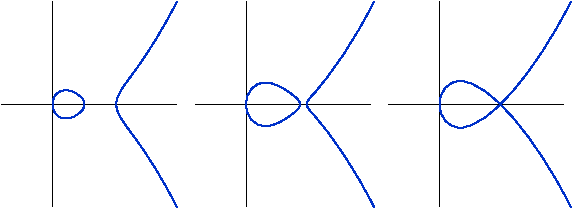
\includegraphics[width=3.6in]{main/cubic-la=0.5,0.9,1}
\centerline{\hfil
\footnotesize
\hbox to 1.15in{\hfil\hfil$\lambda=0.5$\hfil}\enspace
\hbox to 1.15in{\hfil\hfil$\lambda=0.9$\hfil}\enspace
\hbox to 1.15in{\hfil\hfil$\lambda=1$\hfil}\hfil
}
\caption{A curve of genus 1 degenerating to a rational curve with a node
in the family $y^2 = x(x-1)(x - \lambda)$.}
\label{smooth to singular}
\end{figure}


The upshot
is that if we enlarge the original class of curves parametrized by
$M_1$\emdash smooth projective curves of genus 1\emdash to the
slightly larger class
of
irreducible nodal projective curves of
arithmetic genus 1, we still have a coarse moduli space $\overkern31
M_1$ for this slightly larger class of objects. This enlarged moduli
space is obtained by adding one point ``at $\infty$'' to the existing
space $M_1 \cong \AA^1$ to form $\ovM_1 \cong \PP^1` `$.

This is an example of what is called a
\emph{modular compactification}.
\index{modular compactification}%
There is no precise definition, but if we have a
class of objects parametrized by a (noncompact) moduli space $M$ we
may be able enlarge the class of objects to be parametrized, with the
result that the moduli space $\ovM$ of the larger class is
compact.

Modular compactifications of a given moduli problem may or may not exist. It's sometimes a tricky problem to find a suitable class of objects to parametrize: if we don't add enough additional isomorphism classes, not every 1-parameter family of objects in our original class will have a limit in the larger class, meaning the enlarged moduli space will still not be compact; if we add too many,  1-parameter families may have more than one possible limit, meaning the enlarged space won't be separated. For example, in the family
 of curves $C_t$ given as
$$
C_t = V(y^2 -x^3 - t^2x - t^3)
,
$$
the $j$-function
is constant when $t\neq 0$, but  the limiting curve
$C_0$ has a
cusp
(Figure~\ref{smooth to cusp}). This shows that we could not have added
cuspidal curves to $M_1$.

\begin{figure}[b]
\def\quad{\hskip30pt}
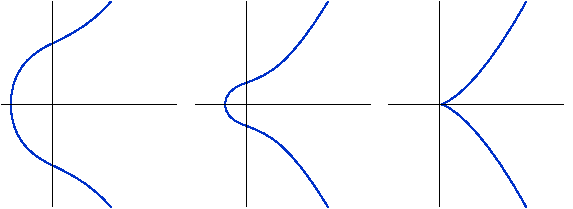
\includegraphics[scale=0.9,viewport=0 0 61 100,clip]{main/cubic-t=0,0.5,1}\quad
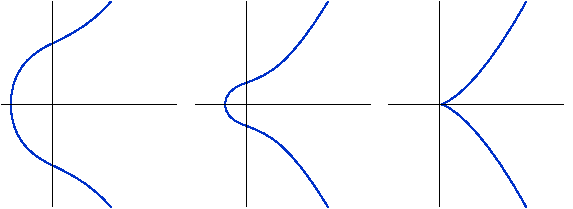
\includegraphics[scale=0.9,viewport=90 0 161 100,clip]{main/cubic-t=0,0.5,1}\quad
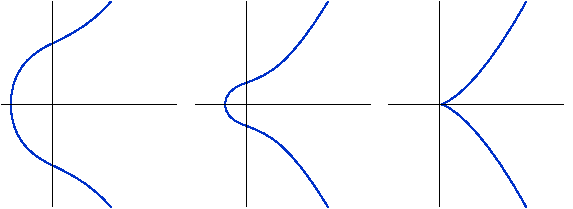
\includegraphics[scale=0.9,viewport=190 0 261 100,clip]{main/cubic-t=0,0.5,1}
\centerline{\hfil
\footnotesize
\hbox to 1.2in{\hfil\hfil$t=1$\hfil}\enspace
\hbox to 1.2in{\hfil\hfil$t=0.5$\hfil}\enspace
\hbox to 1.2in{\hfil\hfil$t=0$\hfil}\hfil
}
\caption{A curve of genus 1 degenerating to a cuspidal curve in the family $
C_t = V(y^2 -x^3 - t^2x - t^3)$.
}
\index{cuspidal curve!of genus 1}%
\label{smooth to cusp}
\label{Fig7.A}
\end{figure}

When modular compactifications do exist, they are extremely valuable
for the study of both the space $M$ and of the objects parametrized
by $M$: compactness allows us to apply the techniques of modern
algebraic geometry to the space $\ovM$, while the fact that
it is still a moduli space gives us a handle on its \null geometry.
In the following section, we will describe a modular compactification
of $M_g$. The objects parametrized are called \textit{stable curves}.

Getting back to the moduli space $\ovM_1$, if we have a family where
$j(\lambda)$ has a pole, we would like to say that the limit of the curves in the family is an irreducible nodal curve,
but this is not necessarily true! For example, the limit of the curves
$$
y^2 = x(x-t)(tx-1)
$$
as $t \to 0$ is reducible, with two components meeting in two points, 0 and $\infty$.
What is true is that a process called
\emph{semistable reduction}
\index{semistable reduction}%
shows that after a base change and a birational
modification of the family around the pole we can replace the family with one where the singular fiber
is indeed an irreducible nodal curve
(Figure~\ref{unstable to stable}).
See \cite{MR1631825} for a description of this process in
general, and several explicit examples.

\begin{figure}
\centerline{\includegraphics[width=2in,height=3in]{"main/Fig07-1"}\llap{\hskip-0.5in
\footnotesize\openup-2pt
\raise100pt\vbox{\hbox{blow down a}\hbox{component}\hbox{of central fiber}}}}
\caption{In this case a birational modification of the
total space of the family changes the unstable reducible curve to a stable curve.}
\label{unstable to stable}
\end{figure}

\section{Higher genus}

The  idea  is  analogous to the one used  for genus 1 curves: to
construct a moduli space, first parametrize curves with a choice of
some additional structure, such as a map to projective space, and then
mod out by the choices made. For any smooth projective curve $C$ of
genus $g\geq 2$, the tricanonical linear series
\index{tricanonical linear series}%
\index{linear series!tricanonical}%
$|3K_C|$ is very
ample; it embeds $C$ as a curve of degree $6g-6$ in $\PP^{5g-6}$. Thus
we have a way of realizing a given abstract curve $C$ as a curve in
projective space, unique up to automorphisms of $\PP^{5g-6}$.

We claim next that the set of smooth, tricanonically embedded curves
is a locally closed subset $X$ of the
Hilbert scheme
\index{Hilbert scheme}%
$\Hilb_{(6g-6)m+1-g}(\PP^{5g-6})$ parametrizing curves of genus $g$
and degree $6g-6$ in $\PP^{5g-6}$. By Lemma~\ref{smooth is open}, the
set of points in the base over which the curves are smooth is open. Let
$$
\Hilb^\circ = \Hilb^\circ_{(6g-6)m+1-g}(\PP^{5g-6})\subset \Hilb_{(6g-6)m+1-g}(\PP^{5g-6})
$$
be this open set.

Next, on the universal family
$\cC \subset \Hilb^\circ \times \PP^{5g-6}$,
we have two families of invertible sheaves: we have the
pullback of $\cO_{\PP^{5g-6}}(1)$; and we have the cube $K^3$ of the
dualizing sheaf. Each gives rise to a section of the relative
Picard variety
\index{Picard variety}%
over $\Hilb^\circ` `$, and the locus where they agree is thus a
closed subset $X \subset \Hilb^\circ` `$.

The group $\PGL_{5g-5}$
of automorphisms of $\PP^{5g-6}$ acts on the variety $X$ and its orbits
\index{PGL@$\PGL_{5g-5}$}%
are the isomorphism classes of smooth curves of genus $g$; thus, we might hope to realize the moduli space $M_g$ as the quotient of $X$ by $\PGL_{5g-5}$. But here things go awry in a hurry: unlike the case of an action of a finite group on a variety,
the orbit spaces of infinite groups are often not algebraic varieties.
(Think of the action of $\CC^*$ on $\CC$ by multiplication.) What is
needed is a tool to extract the ``best possible approximation'' to a
quotient. Happily, David Mumford created a tool that does exactly this:
\emph{geometric invariant theory}
\index{geometric invariant theory}%
\index{Mumford, David}%
(GIT).  To see how GIT can be
used in this  setting to produce the space $M_g$, see the wonderful
introduction in \cite{Mumford-Suominen}
or the more technical version in \cite{MR0450272}.

\begin{theorem}[Mumford]\label{unproved1}
The space of orbits of $\PGL_{5g-5}$ acting on the subset of the Hilbert scheme representing
tricanonical curves has the structure of an algebraic variety $M_g$ which is a \emph{coarse moduli
space} in the
\index{coarse moduli space}%
following
sense:
\begin{enumerate}
 \item Given any flat family $Y\to B$ of smooth curves of genus $g$ there is a morphism of schemes
$B\to M_g$ sending each closed point $p\in B$ to the point of $M_g$
representing the fiber $Y\!_b$.
 \item These maps form a natural transformation from the functor $G(-)$ of families of smooth curves to the functor $\Mor_{\mathrm{ schemes}}(-,@ M_g)$
through which any natural transformation $G \to \Mor_{\mathrm{ schemes}}(-,@ M')$
 factors.
\end{enumerate}
\end{theorem}

The power of the theory of the moduli space of curves was greatly increased when compactifications of the space (there are many interesting ones) were introduced. One of these, the compactification
\index{modular compactification}%
of $M_1 = \AA^1$ to $\ovM_1 = \PP^1$ by adding a nodal curve, has already been mentioned. This has the desirable properties that the subset added to $M_1$ is a divisor; and the compactification is \emph{modular} in the sense
that the point added corresponds to a curve almost of the same type as the curves in $M_1$.

There are two reasons why a compactification is  important:
\index{compactification}%
\index{compactification|seealso modular}%

First, the great majority of the techniques that algebraic geometers
have developed for dealing with varieties apply directly only to
projective varieties. For example, the
Satake compactification
\index{Satake compactification}%
is a projective variety containing $M_g$ in such a way that the
complement\emdash usually referred to as the
boundary\emdash has
codimension 2. Taking successive hyperplane sections that pass through
a given point but don't meet the boundary, we see that for $g\geq 2$
there is a complete one-dimensional family of \emph{smooth} curves
containing any smooth curve of genus $\geq 2$.

Often, though, we can learn the most from a compactification where the
added boundary
is a divisor, and this is the case for the Deligne--Mumford compactification
\index{Deligne--Mumford compactification}%
$\ovM_g$, described below,  introduced
in the
groundbreaking 1969 paper \cite{Deligne-Mumford}.
A central example of how this is used is given in
Section~\ref{mgunirational}, where we take up the question, ``can we
write down a general curve of genus $g$?''

To describe this compactification, we first explain some of the language and results of geometric
invariant theory.

\subsection*{Stable, semistable, unstable}

Given a quasiprojective variety $X \subset \PP^N$ and a group $G \subset \PGL_{N+1}$ that carries $X$ into itself, we wish to construct as good a map as possible from the set of orbits
to a projective space. Whatever map we take, the closure of the
image will correspond to a graded ring. We want to preserve as much of the structure of the orbit space as possible, and on an open affine cover
this means finding as many functions as possible that are invariant on
the orbits. Thus it is natural to take the
ring of invariants
\index{invariant!ring of --s}%
\index{ring of invariants}%
of the homogeneous coordinate ring $A$ of the closure of $X$ as the homogeneous coordinate ring of the closure
of the image of $X$.

The first difficulty is that the elements of $A$ are not functions on $X$, so $G$ may not even act on $A$. However,
it is possible to lift the action of $G$ to an action on $A$ of the
slightly larger group, $\SL_{N+1}$, a process called
\index{linearization}%
\emph{linearization}. The kernel of the map $\SL_{N+1} \to \PGL_{N+1}$
consists of diagonal matrices of finite order dividing $N+1$, and the choice of
a linearization amounts to a choice of a character of this abelian
group. However, the choice doesn't
matter,
since the kernel acts trivially on forms of degree a multiple
of $N+1$,
and thus
the action of $\PGL_{N+1}$ itself  extends to an action on the
homogeneous coordinate ring of the $(N+1)$-st Veronese embedding.
Another way to say this is to introduce the cone $\overkern31 X
\subset \AA^{N+1}$ over $X$; a linearization amounts to an action of
$\SL_{N+1}$ on $\overkern31 X$.%
{\meshing\par}

The second difficulty in this program is that the ring of invariants
of an infinite group may not
be finitely generated,
so it may not correspond to a projective variety. Hilbert showed that if $G= \SL_{N+1}$, then the ring of invariants
is finitely generated. Since Hilbert's time this result has been extended to the class of
\emph{linearly reductive}
\index{linearly reductive group}%
groups\emdash see \cite{MR0382294}.
Thus the subring $A^G \subset A$ of invariant elements is finitely generated over the ground field.

The third difficulty is that the points of $\Proj(A^G)$, usually
\index{'/'@$\quot$|defi}%
denoted $X\quot G$, are generally not in one-to-one correspondence
with the orbits of $G$ on $X$!

Geometric invariant theory explains the relationship of $X\quot G$ to the set of orbits. To do this, it performs a sort of triage on the points of $X$ (or their orbits), dividing them into three classes: stable, semistable and unstable. The theory also provides tools for determining this stratification.


\begin{enumerate}
\item  \emph{Stable points}. These are the points whose orbits in
\index{stable point|defi}%
$\AA^{N+1}$ are closed. They comprise an open subset
$X^{\mathrm{stable}} \subset X$, and the points of an open subset of
$X\quot G$ correspond one-to-one to the stable orbits, that is, an open subset
\index{set-theoretic equality}%
that is
set-theoretically
$X^{\mathrm{stable}}/G$. In general, this
set may be empty, but in the case of the action of
$\PGL_3$
on the
\index{PGL@$\PGL_3$}%
$\PP^9$ of
plane cubics,
\index{plane cubic}%
the stable points are the smooth plane
cubics, and the quotient is the affine $j$-line.

\index{stable points}%
\item \emph{Strictly semistable points}.
\index{semistable points|defi}%
\index{strictly semistable points|defi}%
These are the points $p$ such that there exists an invariant form not
vanishing at $p$.  Together with the stable points, comprise a larger
open subset $X^{\mathrm{{semistable}}} \subset X$, called the
\emph{semistable} locus. Two  semistable points $p,q$ map to the same
point in $X\quot G$ if and only~if $\overkern20{Gp}\cap
\overkern20{Gq}\cap X^{\mathrm{{semistable}}} \neq \emptyset$. In the
example of the action of $\PGL_3$ on  $\PP^9` `$, the semistable
locus contains  the orbits of smooth and nodal plane cubics; that is,
smooth cubics together with the three orbits consisting of irreducible
cubics with a node, unions of lines and conics meeting transversely,
and triangles. In the quotient, these last three orbits correspond to
just one additional point, and this quotient is the
compactification of the affine line
\index{compactification!of the affine line}%
to the projective line obtained by adding one point.

\item  \emph{Unstable orbits}. These are the
\index{unstable points|defi}%
points $p$ on which all invariant polynomials vanish, so that the induced map
$\Proj A \to \Proj (A^G)$ is not even defined at $p$. Thus unstable
points do not correspond to any points of $X\quot G$; in fact, they
cannot be included in any topologically separated quotient of an open
subset of $X$ defined in this way, though there may be other
compactifications, coming from
other representations of $M_g$ as $X'\quot  G'$; see \cite{MR3044128}.
\end{enumerate}

\section{Stable curves}

The compactification $\ovM_g$ is also a
\emph{modular} compactification
\index{modular compactification}%
\index{compactification!modular}%
in the sense that the points of the boundary correspond to slightly more
\index{stable curves}%
general objects of the same type as the points of $M_g$.

\begin{definition}
A reduced irreducible connected curve is \emph{stable}
\index{stable curve|defi}%
if it has at most nodes as singularities and if every smooth rational
component meets the other components at least three times
(Figure~\ref{complicated stable curve}).

\begin{figure}[b]
\centerline {\includegraphics[height=1.2in]{"main/Fig07-2"}}
\caption{A stable curve.}
\label{complicated stable curve}
\end{figure}

The last phrase of the definition could be replaced by the equivalent condition that the automorphism group
of $C$ is finite.
\end{definition}

These are stable points in the Hilbert scheme of tricanonical
embeddings in the sense of geometric invariant theory, and the result
is that $M_g$ has a modular compactification that is a
projective variety:

\begin{theorem}[properties of $\ovM_g$
\cite{Deligne-Mumford,MR702954}]%
\hskip-20pt % first item shouldn't run inline because the headline is full
\label{DM is coarse}%
\begin{enumerate}
 \item $\ovM_g$ is a projective variety.
 \item The points of $\ovM_g$ correspond one-to-one to isomorphism classes of smooth curves.
 \item For every family $\cC \to B$ of stable curves there is a morphism of schemes $B\to M_g$ carrying
 each closed point  $b \in B$ to the point representing the isomorphism class of the fiber of $\cC$ over $b$.
 These maps form a natural transformation from the functor $G(-)$ of families of stable curves to the functor
$$\Mor_{\mathrm{ schemes}}(-,@ \ovM_g)$$
through which any natural transformation $G \to \Mor_{\mathrm{ schemes}}(-,@ M')$
 factors.
\end{enumerate}
\end{theorem}

The deepest theorems about $M_{g}$ have been proven using the
divisor class group
\index{divisor class group}%
 of $\ovM_{g}$,
and many of the divisors that play a role are actually supported on
the complement $\ovM_{g} \setminus M_{g}$, often called the
\emph{boundary}.
\index{boundary|defi}%
{\meshing\par}

\begin{fact}
\it
For $g\geq 1$ the boundary $\ovM_{g}\setminus M_{g}$ is the
union of $@1+\lfloor{g/2}\rfloor$ divisors whose generic points are
\begin{enumerate}
 \item irreducible nodal curves of geometric genus $g-1$
and
 \item for $@i = 1, \dots,\lfloor{g/2}\rfloor$
the union of two smooth curves $C_{i}\cup C_{g-i}$ of genera
 $i$ and $g-i$ meeting in a point.
\end{enumerate}
\vskip-1.4\baselineskip
\end{fact}

We will not prove either of Theorems~\ref{unproved1}
and~\ref{DM is coarse}. For an introduction to the
proofs, with references, see \cite{MR1631825}.

\subsection*{How we deal with the fact that $\ovM_g$ is not fine}

The fact that $\ovM_g$ is not a fine moduli space\emdash and that
correspondingly
there does not exist a universal family
\index{universal family!nonexistence}%
of curves over
it\emdash is unquestionably a nuisance. Nonetheless, there are ways of
dealing with the situation. The first step is to identify the cause of
the problem, which is that some curves have nontrivial automorphisms.
There are three ways to proceed:
\index{automorphism}%

\begin{enumerate}
\item \emph{Kill the automorphisms}. The idea here is to add
additional structure to the objects parametrized, so as to eliminate
automorphisms. Here is an example of such a construction. We saw in
Chapter~\ref{JacobianChapter} that on a smooth projective curve $C$
of genus $g$, the collection of invertible sheaves $\cL$ with $\cL^m
\cong \cO_C$ forms a group isomorphic to $(\ZZ/m)^{2g}$. We define a
\emph{curve with level $m$ structure}
\index{curve!with level $m$ structure|defi}%
to be such a curve, together with a choice of $2g$ generators
$\cL_1,\dots,\cL_{2g}$ for this group. On every curve $C$ of genus
$\geq 2$ an automorphism fixing all line bundles of order $m \geq 3$
is trivial, and there does
exist a fine moduli space $M_g[m]$
\index{M@$M_g[m]$}%
for curves with level $m$ structure; this space is a finite cover of
$M_g$. Thus, while a universal family does not exist over $M_g$, one
does exist over a finite cover of $M_g$, and this is sufficient for
many purposes.

\item \emph {Ignore the automorphisms}.
Here we use a basic fact, which we'll establish in Section~\ref{curves with automorphisms}: in $M_g$, the locus $A \subset M_g$ of curves that do have automorphisms other than the identity has codimension $g-2$. If we restrict to the complement $M_g^\circ = M_g \setminus A$, accordingly, there does exist a universal family, and again this is sufficient for many purposes; for example, if $g \geq 4$ then a divisor class on $M_g$ is determined by its restriction to $M_g^\circ$, so we can just work over that open set.

\item \emph{Embrace the automorphisms}. We mentioned above that there
  does not exist a fine moduli space for curves of genus $g$ in the
  category of schemes. But there is a larger category, called
\emph{stacks},
\index{stack}%
in which a fine moduli space does exist. This solution to the problem, pioneered by Deligne and Mumford, has
many advantages but involves a substantial investment in mastering the technical issues; readers who wish to pursue this avenue may consult \cite{Deligne-Mumford}, \cite{Olsson}, or the forthcoming book {\it Stacks and moduli} by Jarod Alper.
\index{Alper, Jarod}%
\end{enumerate}


\section{Can one write down a general curve of genus $g$?}\label{mgunirational}

We have made a fuss over the value of compactifying $M_g$ to a projective variety. To see an example of the usefulness of $\ovM_g$, we'll take up a question we've raised before: Can one write down a general curve of genus $g$?
More precisely,  does there exist a family of curves depending freely
on parameters that includes all the curves in an open subset of
$M_{g}$,
as the equation $y^{2} = x(x-1)(x-\lambda)$
represents general curves of genus 1? Still more precisely,
we say that a variety is \emph{unirational}
\index{unirational|defi}%
if it admits a
dominant morphism
\index{dominant map}%
from an open subset of $\AA^{n}$.
Our question is: Is $M_g$ unirational?

We have produced  families with free parameters in genera 2 and 3. Essentially
the same approach works in genera $4$ and $5$; in each case a general
canonical curve is a
complete intersection,
\index{complete intersection}%
so that if we take the coefficients of its defining polynomials to be
general scalars we have a general curve.

This method breaks down when we get to genus 6, where a canonical curve is not a complete intersection. But it's close enough: as discussed in Chapter~\ref{Brill--Noether}, a general canonical curve of genus 6 is the intersection of a smooth del Pezzo surface $S \subset \PP^5$ with a quadric hypersurface $Q$; since all smooth del Pezzo surfaces in $\PP^5$ are isomorphic, we can just fix one such surface $S$ and let $Q$ be a general quadric.

It gets harder as the genus increases. Already genus 7 calls for a
different approach. Here we want to argue that, by
Brill--Noether theory,
\index{Brill--Noether theory}%
a general curve of genus $7$ can be realized as (the normalization of)
a plane
septic curve
\index{septic curve}%
with 8 nodes $p_1,\dots,p_8 \in \PP^2` `$. Conversely, if $p_1,\dots,p_8 \in \PP^2$ are general points then having nodes at the points $p_i$ imposes $ 3\times 8 = 24$ independent conditions on the $\PP^{35}$ of curves of degree 7, so that we would expect that the septic curves double at the $p_i$ form a linear series, parametrized by a projective space $\PP^{11}$.

This suggests that we consider the space
$$
\Sigma \colonequals \bigl\{@ (p_1,\dots,p_8,C) \in (\PP^2)^8 \times \PP^{35} 
\mid C \text{ is singular at } p_1,\dots,p_8 @\bigr\}
$$
With a little work, we can see that there is a unique component $\Sigma^\circ$ of $\Sigma$ dominating $(\PP^2)^8` `$, which is a $\PP^{11}$-bundle over an open subset of $(\PP^2)^8$ and hence rational; this component dominates $M_7$, showing that $M_7$ is unirational.

A similar approach works through genus 10, and Severi conjectured that
\index{Severi, Francesco}%
it would be possible to do something similar for all genera. The
approach through plane curves, however, fails in genus 11: by the
Brill--Noether theorem,
\index{Brill--Noether theorem}%
the smallest degree of a planar embedding of a general curve of genus
11 is 10; by Theorem~\ref{grd omnibus} (itself a consequence of
the Brill--Noether theorem), such a curve has $\tbinom{9}{2}-11 = 25$
nodes. But $3 \times 25 > 65$, the dimension of the space of plane
curves of degree 10. Thus, if we introduce the analogue of the
incidence correspondence
\index{incidence correspondence}%
we used in the case of genus 7\emdash that is,
$$
\Sigma \colonequals\bigl\{@(p_1,\dots,p_{25},C)\in(\PP^2)^{25} \times \PP^{65} 
\mid C \text{ is singular at } p_1,\dots,p_{25} @\bigr\}
$$
\emdash
then the projection $\Sigma \to (\PP^2)^{25}$ is not dominant, and we have no idea if $\Sigma$ is rational.
Ad hoc (and much more difficult) arguments have been given in genera
11, 12, 13 and 14, but so far no-one can go further in producing
general curves; in genus 15 it is only known that
 any two general curves can be 
\null connected by a chain of rational curves that passes through
the locus of irreducible nodal curves in $\ovM_{g}$
\cite{MR2202246}. In genera 15 and 16 Chang and Ran showed
the  weaker statement
that $\ovM_{g}$ has no pluricanonical divisors.%
\looseness=-1
{\meshing\par}

However the issue is resolved for all genera $\geq 22$. Surprisingly, this depends (in the current state of our knowledge) on an understanding of the complement
$\ovM_{g}\setminus M_{g}$ and its image in the divisor class group of
$\ovM_{g}$. The starting point is the fact that a smooth
$n$-dimensional projective variety $X$ with an effective
pluricanonical canonical divisor\emdash that is, a nonzero section of
the sheaf $\omega_{X}^{\otimes p}$ for some $p>0$\emdash cannot be
unirational: if there were a
dominant rational map
\index{dominant map}%
$\PP^n \to X$, we
could pull this section back to get an effective pluricanonical
divisor on $\PP^n` `$, which doesn't exist because
the canonical divisor on $\PP^{n}$ has negative degree. At the same
time, we can analyze the divisor class theory of the space $\ovM_g$
and for large $g$ exhibit an effective pluricanonical divisor on $M_g$
by using components of  $\ovM_{g}\setminus M_{g}$.
The upshot is this:

\begin{npt}
\begin{theorem}[\cite{Harris-MumfordModuli,HarrisModuli,Eisenbud-HarrisModuli,M22-23}]
For all $g \geq 22$, $M_g$ is not unirational.
\unif
\end{theorem}
\end{npt}

In each case, what is actually proven is the stronger but more
technical statement that $\ovM_g$ has \emph{general type}.
\index{general type}%
This line of argument requires a great deal of work; the interested reader
can find more details, plus a guide to the literature, in
\cite{MR1631825}.

\section{Hurwitz spaces}\label{Hurwitz spaces}

Hurwitz spaces are spaces parametrizing branched covers. They are fascinating objects; we know quite a bit about their geometry but there is much that is unknown as well. In this discussion, we'll stick to the simplest case, that of the \emph{small Hurwitz spaces}, parametrizing simply branched covers of $\PP^1` `$.
\index{Hurwitz space|(}%
\index{simply branched cover}%

To start with the definition: the small Hurwitz space $\Hur^\circ_{g,d}$
\index{Hur@$\Hur^\circ_{g,d}$|defi}%
parametrizes pairs $(C, f)$ where $C$ is a smooth
curve of genus $g$ and $f : C \to \PP^1$ a map of degree $d$ with
simple branching; that is,
$$
\Hur^\circ_{g,d} = \bigl\{@(C, f) \mid C \in M_g
\text{ and } f:C \to \PP^1 \text{ simply branched of degree } d@\bigr\}.
$$

There are two natural maps from the Hurwitz space to other spaces.
First, we can ``project on the first factor;'' that is, simply forget
the map $f$ to arrive at a map $\pi : \Hur^\circ_{g,d} \to M_g$.
Secondly, we can associate to a point $(C,f) \in \Hur^\circ_{g,d}$ the
branch divisor $B \subset \PP^1` `$, which is an unordered $b$-tuple
of distinct points in $\PP^1` `$, which we can think of as a point in
the $b$-th symmetric product $(\PP^1)_b  \cong \PP^b` `$. We thus have
a diagram
\vspace*{-10pt} % meshing
$$
\small
\xymatrix@C=15pt@R=25pt{
 & \Hur^\circ_{g,d} \ar[ld]_\pi  \ar[rd]^\beta & \\
M_g  & & U \subset \smash{\PP^b}
}
\index{beta@$\beta$ (Hurwicz spaces)}%
$$
where $U \subset \PP^b$ is the complement of the hypersurface in $\PP^{b}$ where at least 2 of the
$b$ points are equal, called the
discriminant hypersurface.
\index{discriminant hypersurface|defi}%
Thus the Hurwitz space is positioned between an object $U$ we
understand relatively well, and an object $M_g$ about which we would
like to know more; this accounts for the historical importance of
Hurwitz spaces. We'll now illustrate how this can be exploited.

To begin with, by the analysis in Section~\ref{branched covers}, we
see that \emph{the map $\beta$ is a covering space}: for any reduced
divisor $B \subset \PP^1$ there are a finite number of simply branched
covers of $\PP^1$ with branch divisor $B$; and as we vary the points
of $B$ locally we can deform the cover along with them. This allows us
to give the Hurwitz space $\Hur^\circ_{g,d}$ the structure of a smooth
variety, and also tells us that
$$
\vspace*{-4pt}
\dim(\Hur^\circ_{g,d}) = b = 2d+2g-2.
\vspace*{-4pt}
$$

\subsection*{The dimension of $M_g$}

Next, we look at the projection $\pi : \Hur^\circ_{g,d} \to M_g$. To
\index{M0g@$M_g$!dimension}%
start, let's assume $d$ is large relative to $g$; $d \geq g+1$
suffices, but you can take $d$ as large as you like; taking $d > 2g$
may make the argument simpler.

\begin{proposition}
If $d \geq g+1$, the map $\pi :
\Hur^\circ_{g,d} \to M_g$ is surjective, with fibers of dimension $2d-g+1$.
\end{proposition}

\begin{proof}
The question is, how many simply branched maps $f : C \to \PP^1$ of
degree $d$ are there
for a given curve $C$?
To begin with, the
$g+1$ theorem
\index{g plus 1@$g+1$ theorem}%
(Theorem \ref{g+1 theorem}) tells us that
there are some, whence we see that $\pi$ is surjective.

We can compute the dimension of the fibers, too.
\kern-1pt To specify a map
$f {:}@ C {\to} \PP^1`$,
we can start by choosing a divisor $D \in C_d$, which
will be the divisor $f^{-1}(\infty)$; this can be a general divisor of
degree $d$ on $C$. Second, we choose a divisor $E$ which will be
$f^{-1}(0)$; this can be a general member of the linear system $|D|$,
which has dimension $d-g$. Finally, specifying $f^{-1}(\infty)$ and
$f^{-1}(0)$ determines the map $f$ up to scalar multiplication on
$\PP^1$; adding up the degrees of freedom, we see that the fibers of
$\pi$ have dimension
$$
d + (d-g) + 1 = 2d-g+1.
\qed
$$
\let\qed\relax
\end{proof}

Finally, we conclude that if $g\geq2$ then
$$
\dim(M_g) = (2d+2g-2) - (2d - g + 1) = 3g-3.
$$

We can use this in turn to analyze the cases of smaller $d$. As a
basic application, note that the group $\PGL_2$ of automorphisms of
$\PP^1$ acts on the Hurwitz space: given $\varphi \in \PGL_2$, we can
send $(C,f)$ to $(C, \varphi \circ f)$. Moreover, the orbits of this
action lie in fibers of the projection $\pi : \Hur^\circ_{g,d} \to M_g$,
meaning that the fibers of $\pi$ have dimension at least 3.

\begin{corollary}\label{branched cover BN}
If $d < \bigl\lceil \frac{g}{2} \bigr\rceil + 1$, then a general curve
$C$ of genus $g$ does not admit a map of degree $d$ to $\PP^1` `$.
\unif
\end{corollary}

This is one-half of the case $r=1$ of the
Brill--Noether theorem,
\index{Brill--Noether theorem}%
about which we will say much more later.

\subsection*{Irreducibility of $M_g$}

Another important application is the original proof of the
\index{Hurwitz, Adolf}%
\index{M0g|$M_g$!irreducibility}%
irreducibility of $M_g$. Hurwitz \citeyear{Hurwitz} analyzed the
\index{monodromy}%
\index{historical context}%
monodromy of the map $\beta: \Hur^\circ_{g,d} \to U \subset\PP^b$,
which describes what happens
when you let the branch
points of a cover wander around in $U$ before coming back to their
original locations. He proved that the monodromy is transitive, and
hence that the Hurwitz space $\Hur^\circ_{g,d}$ is irreducible; since
$\Hur^\circ_{g,d}$ dominates $M_g$ for $d$ large, he deduced that $M_g$
must be irreducible as well.

Hurwitz's argument illustrates a fundamental point: in practice,
moduli spaces of curves ``with extra structure,'' such as a map to
projective space, are often easier to work with, and provide a useful
tool for understanding the geometry of abstract moduli spaces. Given an abstract curve $C$ of genus $g$, it's
hard without developing a fair amount of deformation
theory, to show that $C$ varies in a nontrivial family. But if
$C$ is expressed as a branched cover, we can find such families just
by varying the branch points.

There are many open problems connected with the Hurwitz scheme; here are a few:
\begin{enumerate}
\item A compactification of the Hurwitz scheme by
\index{admissible cover}%
\emph{admissible covers}
(allowing both source and target
of the covering to be reducible in a controlled way) is known \cite{MR1631825}, but the boundary is very complicated, and it would be interesting to find a simpler one.

\item It is conjectured that the
Picard group
\index{Picard group}%
of the Hurwitz scheme is torsion; see \cite{MR3320849},
where the conjecture is proved
for $g\leq 5$, and \cite{mullane} for the case $d>g-1$.

\item There is active work and many open problems around computing the
\emph{Hurwitz numbers},
\index{Hurwitz number|defi}%
that is,
the number of curves having maps to $\PP^{1}$ with specified degree and branching; see for example \cite{Hurwitz2} and \cite{ELSV}.
\index{Hurwitz space|)}%
\end{enumerate}

\section{The Severi variety}\label{severi variety}

Despite having been studied for so long, many questions about plane
curves remain open\emdash for example: which ones degenerate into
which others, and in what way. All plane curves of degree $d$ have the
same Hilbert function, and thus the same
arithmetic genus
\index{arithmetic genus}%
$\tbinom{d-1}{2}$, but since curves of degree $d$ can have different
sorts and numbers of singularities, they can have geometric genera
from 0 to $\tbinom{d-1}{2}$. In this section we will explore the
subset of (reduced, irreducible) curves of degree $d$ with a fixed
\index{geometric genus}%
geometric genus. We will focus on the open set consisting of
nodal curves (those with only nodes as singularities),
and compute its dimension.

\def\Vdg{V_{\mskip-6mu d,g}}
\def\Vdgbar{\overkern1{17}{\Vdg}}
\def\Vdgpbar{\overkern1{19}{V_{\smash{\!d,g'`}}}}

Let $\PP^N \colonequals  \PP^{\sbinom{d+2}{ 2} - 1}$ be the projective space parametrizing plane curves of degree $d$.
Within $\PP^N$ the set of reduced irreducible curves is open\emdash it is the complement of the union of the images of the maps
$$
\PP^{\sbinom{d_1+2}{ 2} - 1}\times\PP^{\sbinom{d_2+2}{ 2}-1} \to \PP^N
$$
with $d_1+d_2 = d$ given by multiplication of forms.

\begin{definition}
The \emph{Severi variety}
\index{Severi variety|defi}%
$\Vdg \subset \Vdgbar$ is the locus of irreducible plane curves of
\index{V0gd@$\Vdg$|defi}%
degree $d$ with $\delta = \tbinom{d-1}{2} - g$ nodes and no other
singularities. This is a locally closed subset of $\PP^N` `$.
(Reason: having only nodes as singularities is an open condition; having at least a certain number of them
is a closed condition.)
It is sometimes
\index{small Severi variety|defi}%
called the \emph{small Severi variety}, since we are excluding curves with more complicated singularities.
\end{definition}

We will see that the closure $\Vdgbar$ is well behaved in a
neighborhood of $\Vdg$; but away from this, even the singularities
of $\Vdgbar$ are not well understood. It
is an interesting open
problem to find a simpler partial compactification of $ \Vdg$.

\begin{fact}\label{severi irreducible}
Corollary~\ref{local geometry of Severi} says that
the variety $\Vdg$ is smooth. In 1921 F. Severi gave an incorrect
proof
that $\Vdg$ is
connected, and thus irreducible.
\index{Severi, Francesco}%
\index{historical context}%
A~correct proof was finally given in \cite{MR837522}.
\end{fact}


\subsection*{Local geometry of the Severi variety}

We first consider the
\index{universal singular point}%
\index{Severi variety!local geometry}%
universal singular point
$$
\Phi \colonequals  \left\{ (C, p) \in \PP^N \times \PP^2 \mid p \in C_{\sing} \right\}
$$
and its image $\Delta\subset \PP^N` `$, the \emph{discriminant variety}.
\index{discriminant variety}%

\begin{proposition}
\label{local severi geometry}
 $\Phi$
is smooth and irreducible of dimension $N-1$,
and the discriminant $\Delta$ is a hypersurface in $\PP^N` `$.
\unif
\end{proposition}

\begin{proof}
Projection on the second factor expresses $\Phi$ as a $\PP^{N-3}$-bundle over $\PP^2` `$. Explicitly, if $[X,Y,Z]$ are homogeneous coordinates on $\PP^2` `$, and $\{a_{i,j,k} \mid i+j+k = d \}$ are homogeneous coordinates on $\PP^N` `$, then the universal curve
$$
\CC \colonequals  \left\{ (C, p) \in \PP^N \times \PP^2 \mid p \in C \right\}
$$
is given as the zero locus of the single bihomogeneous polynomial
$$
F([a_{i,j,k}], [X,Y,Z] ) = \sum a_{i,j,k} X^iY^jZ^k
$$
of bidegree $(1, d)$;
and the universal singular point is the common zero locus of the three partial derivatives $\partial F/\partial X$, $\partial F/\partial Y$ and  $\partial F/\partial Z$.

The set of forms $F$ that define curves singular at a given point is
defined by~3 independent linear conditions, and since the set of
points is 2-dimensional,
the set $\Delta$ of singular forms has dimension $N-1$.
\end{proof}

We next compute the differential of the map $\pi : \Phi \to \PP^N$:

\begin{lemma}\label{tangent space to discriminant}
Suppose that $(C,p)\in \Phi$, with $p$ a node of $C$.  The differential
$$
d\pi : T_{(C,p)}\Phi \to T_C \PP^N
$$
is injective, with image the hyperplane $H_p \subset \PP^N$ of plane curves containing the point $p$.
\end{lemma}

Thus, if $p$ is a node of $C$ and the only singularity of $C$, then $\Delta$ is smooth at $C$; and more generally the image of a small analytic neighborhood of $(C,p) \in \Phi$ is smooth, and we can identify its tangent space at $p$ with the hyperplane $H_p$.

\begin{proof}
We will prove this using affine coordinates on $\PP^2$ and $\PP^N` `$.
Changing coordinates if necessary, we may assume that the point
$[1,0,0]$ is not in $C$, and that the point $p$ is $[0,0,1]$.
Let $x = X/Z$ and $y = Y/Z$ be coordinates on the affine plane $Z \neq 0$ and
write the polynomial $F(x,y,1)$ above as
$$
f(x,y) = \sum_{i+j \leq d} a_{i,j} x^iy^j
,
$$
with $a_{d,0}$ normalized to 1.

Let $g,h$ be the two partial derivatives of $f$:
\begin{align*}
 g(x,y) \colonequals  \frac{\partial f}{\partial x} &= \sum_{i+j \leq d} i a_{i,j} x^{i-1}y^j\\
h(x,y) \colonequals  \frac{\partial f}{\partial y} &= \sum_{i+j \leq d} j a_{i,j} ix^{i}y^{j-1}.
\end{align*}
The functions $f, g$ and $h$ are local defining equations for $\Phi$;
we consider their partial derivatives with respect to $x, y$ and
$a_{0,0}$, evaluated at the point $(C,p)$, as in
the table:
$$
     \begin{array}{lccc} % <-- Alignments: 1st column left, 2nd middle and 3rd right, with vertical lines in between
            & f & g & h \\
      \hline
\vbox to 11pt{} %strut
\unfrac{\partial}{\partial x} & 0 & a_{2,0} & a_{1,1} \\
\unfrac{\partial}{\partial y} & 0 & a_{1,1} & a_{0,2} \\
\unfrac{\partial}{\partial a_{0,0}} & 1 & 0 & 0
    \end{array}
$$

The fact that $p$ is a node of $C$ (and not a more complicated singularity) implies that the upper right $2 \times 2$ submatrix is nonsingular, which shows that the differential $d\pi$ is injective, and its image is the hyperplane $a_{0,0} = 0$ in $\PP^N` `$, which is exactly the hyperplane of curves containing $p$.
\end{proof}

\begin{lemma}\label{adjoint independent}
The nodes $q_i$ of an irreducible nodal plane curve $C$ of degree $d$
\index{node!condition imposed by}%
\index{independent conditions}%
impose independent conditions on curves of degree $d-3$, and hence on
curves of any degree $m \geq d-3$.
\end{lemma}

\begin{proof}
We will prove in Chapter~\ref{PlaneCurvesChapter} that the $g$ sections of the canonical sheaf on the normalization $\widetilde C$ of
$C$ are the preimages of the sections of $\sO_C(d-3)$ that vanish at the nodes. On the other hand,
$h^0(\sO_C(d-3)) = \tbinom{d-1}{2}$, and the difference is exactly the number of nodes.
\end{proof}

\begin{corollary}\label{local geometry of Severi}
\hskip-1.6pt
If $C$ is a nodal curve of degree $d$
and
geometric genus
$g =\nobreak \tbinom{`d-1` `}{2}-\nobreak\delta$, then in a neighborhood of $C\in \PP^N$
the discriminant hypersurface of all singular curves consists of $\delta$ smooth sheets, meeting transversely, and hence
$\Vdg$ is smooth.

In a neighborhood
of
 $C \in \PP^N$
the variety
$\Vdgpbar$
with $g' =  \tbinom{d-1}{2}-\delta' >g$
is the union of $\tbinom{\delta}{\delta'\!}$ smooth branches, each of
dimension $N - \delta'$, corresponding bijectively with subsets of
$\{p_1,\dots,p_{\delta}\}$ of cardinality $\delta'$.
\meshing
\end{corollary}

Figure~\ref{Severi discriminant} shows the case $\delta=2$,  $\delta' = 1$.
\begin{figure}[b]\label{discriminant of a Severi locus}
\centerline {\includegraphics[height=1.6in]{"main/Fig07-3"}}
\vskip-8pt
 \caption{%
Near
the point corresponding to a plane curve with 2 nodes,
$V_{d,@\protect\sbinom{d-1}{2}-2}$ is the
transverse
intersection of two smooth hypersurfaces.}
 \label{Severi discriminant}
\end{figure}


\begin{proof}
Lemma~\ref{tangent space to discriminant} shows that in an analytic neighborhood of $C\in \PP^N$ the discriminant hypersurface $\Delta$  consists of $\delta$ smooth sheets, each corresponding to one node, and Lemma~\ref{adjoint independent} implies that the tangent spaces to these sheets are linearly independent.
\end{proof}

\begin{corollary}\label{dim Severi}
The  Severi variety $\Vdg$ has pure dimension $N - \delta$, where
$$\delta = \tbinom{d-1}{2} - g.$$
\end{corollary}

In Section~\ref{estimating dim hilb}, we give a heuristic calculation
\index{expected dimension}%
\index{h@$h(g,r,d)$|defi}%
of the ``expected dimension'' $h(g,r,d)$ of the variety parametrizing
curves of degree $d$ and genus $g$ in $\PP^r$:
$$
h(g,r,d) \colonequals  4g-3 + (r+1)(d-g+1) - 1.
$$
The actual dimension of the restricted Hilbert scheme may be quite different. But  Corollary~\ref{dim Severi} shows that in case $r=2$ (as in the case of $r=1$), the actual dimension is always the expected.



\section{Exercises}

\begin{exercise}
Consider the action of $G_m$ on $\PP^3$ given in coordinates by
$$t: (x_0,x_1,x_2,x_3) \mapsto (tx_0,\ tx_1,\ t^{-1}x_2,\ t^{-1}x_3)
$$
for $t\in G_m = \CC^*` `$.
\begin{enumerate}
 \item Show that the ring  of forms in $\CC[x_0, \dots, x_3]$ that are
invariant
\index{invariant forms}%
is generated by
$$
x_0x_3, \ x_0x_2,\ x_1x_3,\ x_1x_2
$$
and thus $\PP^3\quot @G_m\cong \PP^1\times \PP^1` `$.
\item Show that the
unstable locus
\index{unstable locus}%
for this action is the union of the two lines $x_0=x_1=0$ and
$x_2=x_3=0$.
\item Show that the orbits of $G_m$ are the points on the unstable lines and, for each
point $p$ not on an unstable line, a copy of
$\PP^1\setminus \{0,\infty\}\cong G_m$ whose closure is the unique line containing $p$ and
meeting both unstable lines.
\end{enumerate}
\end{exercise}

\begin{exercise}
Consider the action of $G_m$ on $\PP^3$ given in coordinates by
$$t: (x_0,x_1,x_2,x_3) \mapsto (tx_0,\ tx_1,\ tx_2,\ t^{-1}x_3)
$$
for $t\in G_m = \CC^*` `$.
\begin{enumerate}
 \item Show that the ring  of forms in $\CC[x_0, \dots, x_3]$ that are invariant is generated by
 forms
\index{invariant forms}%
$$
F(x_0,  x_1, x_2)x_3
$$
where $F$ is a cubic form on $\PP^2` `$, and thus
$\PP^3\quot@G_m\cong \PP^2` `$, with the embedding given by the
third Veronese map.
\index{Veronese map!third}%
\item Show that the unstable locus for this action is the union of the point  $x_0=x_1=x_2 = 0$ and
\index{unstable locus}%
the plane $x_3=0$.
\item Show that the orbits of $G_m$ are the points on the components of the unstable locus and, for each
point $p$ that is not unstable, a copy of
$\PP^1\setminus \{0,\infty\}\cong G_m$ whose closure is the unique line containing $p$ and the unstable
point. Thus the quotient map is the composition of the linear projection from the unstable point with the 3-uple
embedding.
\end{enumerate}
\end{exercise}

\begin{exercise}\label{not fine 1}
Show from the explicit formula for the
\index{j@$j$-function}%
$j$-function
on page~\pageref{formula for j}
that if $j : B \to M_1 = \AA^1$ is a
map  associated to a family $\cC \to B$ of curves of genus 1, then
every zero of the $j$-function has multiplicity divisible by 3, and
conclude that some maps $B\to M_1$ do not correspond to families of
curves; in particular there is no universal family over $M_1$, and
thus $M_1$ is not a fine moduli space for curves
of genus 1. There is a similar problem at $j(\lambda)=1728$.
\end{exercise}

\begin{exercise}\label{not fine 2}
In Exercise~\ref{not fine 1} we saw a local obstruction to the
\index{universal family!nonexistence over $M_1$}%
existence of a universal family over $M_1$. There is also a global
obstruction, coming from the fact that some genus 1 curves have extra
automorphisms. Show that there is a ``tautological'' family over the
punctured $j$-line $L \colonequals  \AA^1\setminus \{0,1728\}$\emdash
that is, a family
$\sX \to L$ whose fiber over $t$ has $j$-invariant $t$; but show that this family is not universal as follows:

Let $B$ be any curve of genus 1 and $\tau : B \to B$ a translation of
order 2, and let $E$ be a fixed
elliptic curve
\index{elliptic curve}%
(that is, a curve of
genus 1 with a chosen point, so that we may identify the points of $E$
with an abelian group).
Let $\cX\to L$ be the family $E\times B$ modulo the equivalence
relation $(e,b) \sim (-e, \tau(b))$.
The projection to $B/\tau$ has all fibers isomorphic to $E/(\pm) \cong E$. But the family is not
isomorphic to the trivial family $E\times B/\tau \to B/\tau$.
\tohint{8-04}
\end{exercise}


%header and footer for separate chapter files

\ifx\whole\undefined
\documentclass[12pt, leqno]{book}
\usepackage{graphicx}
\input style-for-curves.sty
\usepackage{hyperref}
\usepackage{showkeys} %This shows the labels.
%\usepackage{SLAG,msribib,local}
%\usepackage{amsmath,amscd,amsthm,amssymb,amsxtra,latexsym,epsfig,epic,graphics}
%\usepackage[matrix,arrow,curve]{xy}
%\usepackage{graphicx}
%\usepackage{diagrams}
%
%%\usepackage{amsrefs}
%%%%%%%%%%%%%%%%%%%%%%%%%%%%%%%%%%%%%%%%%%
%%\textwidth16cm
%%\textheight20cm
%%\topmargin-2cm
%\oddsidemargin.8cm
%\evensidemargin1cm
%
%%%%%%Definitions
%\input preamble.tex
%\input style-for-curves.sty
%\def\TU{{\bf U}}
%\def\AA{{\mathbb A}}
%\def\BB{{\mathbb B}}
%\def\CC{{\mathbb C}}
%\def\QQ{{\mathbb Q}}
%\def\RR{{\mathbb R}}
%\def\facet{{\bf facet}}
%\def\image{{\rm image}}
%\def\cE{{\cal E}}
%\def\cF{{\cal F}}
%\def\cG{{\cal G}}
%\def\cH{{\cal H}}
%\def\cHom{{{\cal H}om}}
%\def\h{{\rm h}}
% \def\bs{{Boij-S\"oderberg{} }}
%
%\makeatletter
%\def\Ddots{\mathinner{\mkern1mu\raise\p@
%\vbox{\kern7\p@\hbox{.}}\mkern2mu
%\raise4\p@\hbox{.}\mkern2mu\raise7\p@\hbox{.}\mkern1mu}}
%\makeatother

%%
%\pagestyle{myheadings}

%\input style-for-curves.tex
%\documentclass{cambridge7A}
%\usepackage{hatcher_revised} 
%\usepackage{3264}
   
\errorcontextlines=1000
%\usepackage{makeidx}
\let\see\relax
\usepackage{makeidx}
\makeindex
% \index{word} in the doc; \index{variety!algebraic} gives variety, algebraic
% PUT a % after each \index{***}

\overfullrule=5pt
\catcode`\@\active
\def@{\mskip1.5mu} %produce a small space in math with an @

\title{Personalities of Curves}
\author{\copyright David Eisenbud and Joe Harris}
%%\includeonly{%
%0-intro,01-ChowRingDogma,02-FirstExamples,03-Grassmannians,04-GeneralGrassmannians
%,05-VectorBundlesAndChernClasses,06-LinesOnHypersurfaces,07-SingularElementsOfLinearSeries,
%08-ParameterSpaces,
%bib
%}

\date{\today}
%%\date{}
%\title{Curves}
%%{\normalsize ***Preliminary Version***}} 
%\author{David Eisenbud and Joe Harris }
%
%\begin{document}

\begin{document}
\maketitle

\pagenumbering{roman}
\setcounter{page}{5}
%\begin{5}
%\end{5}
\pagenumbering{arabic}
\tableofcontents
\fi


\chapter{Curves of genus 4 and 5}\label{genus 4, 5 Chapter}

In this chapter we
study
the linear systems that exist on curves of genus 4 and 5, and what this says
about maps to $\PP^r` `$, focusing as usual on the nonhyperelliptic case.

\section{Curves of genus 4}

In genus 4 we
face
\index{genus 4|(}%
a question that the elementary theory based on the Riemann--Roch
formula cannot answer: are nonhyperelliptic curves of genus 4
\index{trigonal}%
\index{cover!3-sheeted}%
\emph{trigonal}, that is, expressible as 3-sheeted covers of $\PP^1$?
The answer will emerge from our analysis in
Proposition~\ref{genus 4 trigonal}.

\subsection*{The canonical model}

Let $C$ be a nonhyperelliptic curve of genus 4. The canonical map $\phi_K : C \hookrightarrow \PP^3$  embeds $C$ as a curve of degree 6 in $\PP^3` `$, and we identify $C$ with the image.  As in previous cases we may describe the homogeneous ideal  $I$ of $C$ by considering the restriction maps
$$
\rho_m : H^0(\cO_{\PP^3}(m)) \; \to \; H^0(\cO_{C}(m)) = H^0(mK_C).
$$
\redden{If}
$m=2$ we have $\h^0(\cO_{\PP^3}(2)) = \tbinom{5}{3} = 10$, while by the
\index{Riemann--Roch theorem}%
Riemann--Roch theorem
$$
h^0(\cO_C(2)) = 12 - 4 + 1 = 9.
$$
Thus $C \subset \PP^3$  lies on at least one quadric surface $Q$. The quadric $Q$ must be irreducible, since any reducible and/or nonreduced quadric must be a union of planes, and thus cannot contain an irreducible nondegenerate curve.
If $Q'\subset\nobreak \PP^3$ is another quadric then, by B\'ezout's theorem,
$Q\cap Q'$ is a curve of degree 4 and thus
cannot
contain $C$. From
this we see that $Q$ is unique, and it follows that $\rho_2$ is surjective.

What about cubics? Again we consider the restriction map
$$
\rho_3 : H^0(\cO_{\PP^3}(3)) \; \to \; H^0(\cO_{C}(3)) = H^0(3K_C).
$$
The space $H^0(\cO_{\PP^3}(3))$ has dimension $\tbinom{6}{3} = 20$, while  the Riemann--Roch formula shows that
$$
h^0(\cO_C(3)) = 18 - 4 + 1 = 15.
$$
It follows that the ideal of $C$ contains at least a 5-dimensional vector space of cubic polynomials. We can get a 4-dimensional subspace as products of the unique quadratic polynomial $F$ vanishing on $C$ with linear forms\emdash these define the cubic surfaces containing $Q$. Since $5 > 4$ we  conclude that the curve $C$ lies on at least one cubic surface $S$  not containing $Q$.
B\'ezout's theorem
\index{B\'ezout's theorem}%
shows that the curve $Q \cap S$ has degree 6; thus it must be equal to $C$.

Let $G=0$ be the cubic form defining the surface $S$. By
Lasker's theorem
\index{Lasker's theorem}%
the ideal $(F,G)$ is unmixed,
and thus is equal to the homogeneous ideal of $C$.

Conversely,
let $C = Q\cap S$ with $Q$ a quadric and $S$ a cubic. By Corollary~\ref{canonical of complete intersection} the canonical sheaf of $C$ is
$$
\omega_C = (\omega_{Q} \otimes \cO_{Q}(3))|_C = \cO_C(-2+3) = \cO_C(1)
,
$$
so $C$ is a canonical curve. Since $C$ is smooth, the quadric and the cubic must meet transversely at points that are nonsingular on each of them. Thus:

\begin{theorem}
\label{canonical genus 4}
The canonical model of a nonhyperelliptic curve of genus $4$ is a
\index{curve!of genus 4!nonhyperelliptic}%
\index{complete intersection!of quadric and cubic in $\PP^3$}%
\index{P^3@$\PP^3$}%
complete intersection of a quadric $Q = V(F)$ and a cubic surface
$S=V(G)$ meeting transversely along nonsingular points of each.
Conversely, any smooth curve that is the complete intersection of a
quadric and a cubic surface in $\PP^3$ is the canonical model of a
nonhyperelliptic curve of genus $4$.\qed
\end{theorem}

Since the quadric surface $Q$ containing the canonical curve $C$
is unique, its rank is an invariant of $C$.
Since $C$ is irreducible and nondegenerate, the quadric cannot be a
double plane or the union of two planes, but it can be singular
(rank~3) or smooth (rank 4). On the other hand, the singularities of a
cubic~$S$ such that $S\cap Q = C$ play no role. Of course $S$ must be
nonsingular along~$C$, since else
$C$ would be singular. We can vary $S$ by adding a multiple of the
equation of $Q$ to the equation of $S$, and since this linear system
of cubics has base locus only along $C$,
Bertini's theorem
\index{Bertini's theorem}%
shows that the general such cubic is nonsingular everywhere.

\subsection*{Maps to projective space}

\subsubsection*{Maps to $\PP^1$}

We can now answer the question we asked at the outset, whether a
nonhyperelliptic curve of genus 4 can be expressed as a 3-sheeted
\index{cover!3-sheeted}%
cover of $\PP^1` `$. This amounts to asking if there are any divisors
$D$ on $C$ of degree 3 with $r(D) \geq 1$; since we can take $D$ to be
a general fiber of a map $\pi : C \to \PP^1` `$, we can for simplicity
assume $D = p+q+r$ is the sum of three distinct points.

By the
geometric Riemann--Roch theorem,
\index{Riemann--Roch theorem!geometric}%
a divisor $D = p+q+r$ on a canonical curve $C \subset \PP^{g-1}$ has
$r(D) \geq 1$ if and only~if the three points $p,q,r \in C$ are
collinear. If three points $p,q,r \in C \subset Q$ lie on a line $L
\subset \PP^3$ then the quadric $Q$ will meet $L$ in at least three
points, and hence will contain $L$. Conversely,  if $L$ is a line
contained in $Q$, then the divisor $D = C \cap L = S \cap L$ on $C$
has degree  3. Thus we can answer our question in terms of the family
of lines contained in $Q$.

Any smooth quadric is isomorphic to $\PP^1\times \PP^1` `$, and
contains two families of lines, or
\index{ruling}%
\emph{rulings}.
On the other hand,
any  quadric of rank 3 is a
cone
\index{cone quadric}%
over a smooth plane conic, and thus
has just one ruling. By the argument above, the pencils of divisors on
$C$ cut out by the lines of these rulings are the $g^1_3$s on $C$.
This proves:

\begin{proposition}\label{genus 4 trigonal}
A nonhyperelliptic curve of genus $4$ may be expressed as a
$3$-sheeted cover of $\PP^1$ in either one or two ways, depending on
whether the unique quadric containing the canonical model of the curve
is singular or smooth.
\unif
\end{proposition}

See Figure~\ref{Fig8.1} for an idea how this might look in
each case.

\begin{figure}
\centerline{\raise3pt\hbox{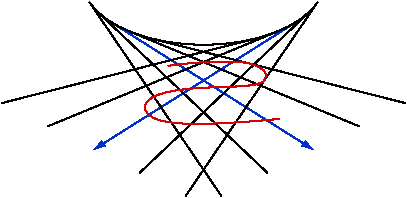
\includegraphics[height=1.93in]{main/Fig08-1}}\hfil
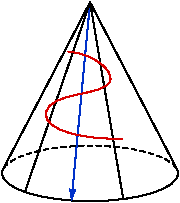
\includegraphics[height=2in]{main/Fig08-2}\quad}
\caption{Left: canonical curve of genus 4 on a smooth quadric, showing
  two $g^{1}_3$s.  Right: canonical curve of genus 4 on a quadric
  cone, with just one~$g^{1}_{3}$.}
\label{Fig8.1}
\end{figure}

Putting together
the analyses of the preceding sections, we have shown that
\index{hyperelliptic-trigonal dichotomy for curves of genus $\leq 4$}%
\emph{every curve of genus $g$ with $2\leq g \leq 4$ is either hyperelliptic or trigonal}.

\subsubsection*{Maps to $\PP^2$}

We can also describe the lowest degree plane models of nonhyperelliptic curves $C$ of genus 4.
We can get a plane model of degree 5 by projecting $C$ from a point $p$ of the canonical model of $C$.
Moreover, the
Riemann--Roch theorem
\index{Riemann--Roch theorem}%
shows that if $D$ is a divisor of
degree 5 with $r(D)=2$ then
$\h^0(K-D) = 1$. Thus $D$ is of the form
$K-p$ for some point $p \in C$, and the map to $\PP^2$ corresponding
to $D$ is $\pi_p$. These  maps $\pi_p: C\to \PP^2$ have the lowest
possible degree (except for those whose image is  contained in a line)
because by
Clifford's theorem
\index{Clifford's theorem}%
a nonhyperelliptic curve of genus 4
cannot have a $g^2_4$.

We now consider the singularities of the
plane quintic
\index{plane quintic}%
$\pi_p(C)$.
Suppose as above that $C = Q\cap S$, with $Q$ a quadric. If a line $L$
through $p$ meets $C$ in $p$ plus a divisor of degree $\geq 2$ then,
as we have seen, $L$ must lie in $Q$.  Any line through $p$ that is
not contained in $Q$ meets $C$ in at most a single reduced point,
whose image is thus a nonsingular point of $\pi(C)$. Moreover, a line
that met $C$ in a divisor of degree 4 or more
would have to lie in both the quadric and
the cubic containing $C$, and therefore would be contained in $C$.
Since $C$ is irreducible there can be no such line; thus the image
$\pi_p(C)$ has at most double points.

We distinguish two cases, depending on whether
the quadric $Q$ is smooth or singular. We will make use of the
Gauss map
\index{Gauss map}%
of the quadric,
described by the next lemma.

\begin{lemma}
Let $L \subset S \subset \PP^3$ be a line on a surface $S \subset \PP^3$ of degree $d \geq 2$, and
write $S_{\sing}$ for the singular locus of $S$. The Gauss map $\cG :
S \to (\PP^3)^*$ sending each point $p \in S\setminus S_{\sing}$ to
the tangent plane $\TT_p(S)$ maps $L$ into the
dual line
\index{dual line!def}%
in $\PP^3$ (that is, the locus of planes containing $L$); if $S$ is
smooth along $L$ then $\cG$  has degree $d-1$, and if $S$ is singular
anywhere along $L$ it has strictly lower degree.
\unif
\end{lemma}

The geometric idea behind this result is easy to understand: If $S$ is
smooth along $L$ and $H\cong \PP^{2}$ is a plane containing $L$, then
$H\cap S = L \cup D$ for a plane curve $D$ of degree $d-1$. The plane
$H$ is tangent to $S$ at a point $p$ if and only~if $H\cap S$ is
singular at $p$; and this occurs at each of the $d-1$ points (counted
with multiplicity) at which $D$ meets $L$, suggesting that the
restriction of the Gauss map is $(d{-}1)$-to-one in this case.

If $S$ is singular somewhere along $L$, then every plane through that point would be among the tangent
planes in the sense above, and the image of $L$ would be a component of a curve of degree $d-1$ containing a line; thus of lower degree.

To see that the multiplicities count correctly in this argument, we will give an algebraic version:
\unif

\begin{proof}
Suppose that in terms of homogeneous coordinates $[X,Y,Z,W]$ on $\PP^3$ the line $L$ is given by $X = Y = 0$. Then the defining equation $F$ of $S$ can be written
$$
F(X,Y,Z,W) = X\cdot G(Z,W) + Y\cdot H(Z,W) + J(X,Y,Z,W)
$$
where $J$ vanishes to order 2 along $L$; that is, $J \in (X,Y)^2` `$. The Gauss map $\cG|_L$ restricted to $L$ is then given by
$$
[0,0,Z,W] \mapsto [G(Z,W), H(Z,W), 0, 0].
$$
The polynomials $G$ and $H$ have degree $d-1$, and have a common zero if and only~if $S$ is singular somewhere along $L$; the lemma follows.
\end{proof}

\begin{example}[Gauss map of a quadric]
\label{Gauss of Quadric}
Let $Q\subset \PP^3$ be a smooth quadric,
\index{Gauss map!of a quadric}%
\index{quadric!Gauss map of}%
and let $L\subset Q$ be the line $X=Y =0$. Since we may write the
equation of $Q$ as $XZ+YW = 0$, the Gauss map of $Q$, restricted to
$L$, maps $L$ one-to-one onto the dual line. Indeed, the
Gauss map
takes $Q$ isomorphically onto its dual, which is also a smooth quadric.

 We can also see this geometrically: if $H \subset \PP^3$ is any plane containing the line $L \subset Q$, then $H$ intersects $Q$ in the union of $L$ and a line $M$; the hyperplane section $Q \cap H = L \cup M$ is then singular at a unique point $p \in L$. Thus the Gauss map gives a bijection between points on $L$ and planes containing $L$.
\unif
\end{example}

Given this, we can analyze the geometry of projections $\pi_p(C)$ of our canonical curve $C = Q \cap S$ as follows:

\begin{enumerate}
\item $Q$ is nonsingular:
In this case there are two lines $L_1, L_2$ on $Q$ that pass through
$p$; they meet $C$ in $p$ plus divisors $E_1$ and $E_2$ of degree 2.
If each $E_i$ consists of distinct points then, since the tangent
planes to the quadric along $L_i$ are all distinct by
Example~\ref{Gauss of Quadric}, the plane curve $\pi(C)$ has two
nodes, one at the image of each $E_i$.

On the other hand, if $E_i$ consists of a double point $2q$ (that is,
$L_i$ is tangent to $C$ at $q\neq p$, or meets $C$ three times at
$q=p$), then $\pi(C)$ has a cusp at the corresponding image point.

In either case, $\pi(C)$ has two distinct singular points, each either a
node or a cusp. The two $g^1_3$s on $C$ correspond to the
projections from these singular points. These possibilities are
illustrated in Figure~\ref{Fig8.2A}.

\begin{figure}[b]
\centerline {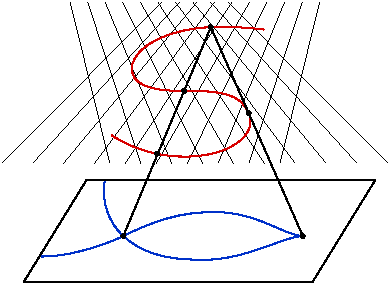
\includegraphics[height=2in]{main/canonical-projected-2}}
\caption{If a genus 4 canonical curve $C$ lies on a smooth quadric, the image of the projection of $C$ from a point $p\in C$
is a
plane quintic
\index{quintic!plane}%
with two singular points.
\hbox to 50pt{} % avoid extra jump before short line
}
\label{Fig8.2A}
\end{figure}

\item $Q$ is a
cone:
\index{cone quadric}%
In this case, since the curve cannot pass through the singular point
of $Q$ there is a unique line $L\subset Q$ that passes through $p$.
Let $p+E$ be the divisor on $C$ in which this line meets $C$. The
tangent planes to $Q$ along $L$ are all the same. Thus if
$E = q_1+q_2$ consists of two distinct points,
the image $\pi_p(C)$ has two smooth branches sharing a common tangent line at
$\pi_p(q_1) = \pi_p(q_2)$. Such a point is called a \emph{tacnode}
(Figure \ref{simplesing})
\index{tacnode}%
of $\pi_p(C)$. On the other hand, if $E= 2q$, that is, if $L$ meets $C$
tangentially at one point $q\neq p$ (or meets $C$ three times at $p$) then
the image curve has a higher-order cusp, called a \emph{ramphoid}
(``beak-like'')
\emph{cusp}
(Figure \ref{ramphoid}).
\index{ramphoid}%
\index{cusp!ramphoid}%
In either case, the one $g^1_3$ on $C$ is the projection from the
unique singular point of $\pi(C)$.
\end{enumerate}

\begin{figure}
\includegraphics[height=1.3in]{"main/ramphoid"}
\caption{A ramphoid cusp on a quartic curve with affine parametrization
$(t^2{+}t^3,t^4)$. Note that the real points of this affine curve lie
entirely in one of the half-planes determined by the tangent line
at the cusp. This was first recorded in a 1744 letter from Leonhard Euler to
Gabriel Cramer,
who had conjectured that for an algebraic curve, the
tangent at a cusp always lies between the two branches.}
\index{Cramer, Gabriel}%
\index{Euler, Leonhard}%
\label{ramphoid}
\end{figure}
\index{genus 4|)}%

\section{Curves of genus 5}

We next consider a nonhyperelliptic curve $C$ of genus 5. There are
\index{genus 5!curve|(}%
now two questions that cannot be answered by simple application of the
Riemann--Roch
theorem:

\begin{enumerate}
\item Is $C$ expressible as a
3-sheeted cover
\index{3-sheeted cover!of $\PP\sp 1$}%
of $\PP^1$?
Equivalently,
does $C$ have a
$g^1_3$?%
\index{g@$g^1_3$}%
\item Is $C$ expressible as a
4-sheeted cover!of $\PP\sp 1$
of $\PP^1$?
In other words, does $C$ have a basepoint free
$g^1_4$?
\index{g@$g^1_4$}%
\end{enumerate}

The first question is answered in the negative by the dimension count
of Section~\ref{Hurwitz spaces}, but the analysis below will give us a
way of characterizing those curves of genus 5 that are trigonal. Note
also that if a curve $C$ of genus 5 is trigonal, the $g^1_3$ on $C$ is
unique: if there were two distinct $g^1_3$s on $C$, with associated
maps $\alpha, \beta : C \to \PP^1` `$, the product map
$$
\alpha \times \beta : C \to \PP^1 \times \PP^1
$$
would give a
birational
\index{birational}%
embedding of $C$ as a curve of
bidegree $(3,3)$
\index{bidegree!$(3,3)$}%
in $\PP^1 \times \PP^1` `$, and it would follow from the genus formula
for curves on $\PP^1 \times \PP^1$ that the genus of $C$ would be at most 4.
\index{P^1 x P^1@$\PP^1 \times \PP^1$|see bidegree}%

The argument of the preceding paragraph can be applied more broadly,
and it's worth stating the results here:

\begin{proposition}\label{general gonality exclusion}
Let $d$ and $e$ be relatively prime integers. If $C$ is a curve of genus $g$ with a basepoint free $g^1_d$ and a basepoint free $g^1_e$, then
$$
g \leq (d-1)(e-1).
$$
The same conclusion holds when $C$ has two distinct
$g^1_d$s with $d$ prime.
\index{g@$g^1_d$, $d$ prime}%
\end{proposition}

\begin{proof}
As before, we let $\alpha$ and $\beta : C \to \PP^1$ be the maps
associated to the $g^1_d$ and the $g^1_e$. In either case
the
product map $\alpha \times \beta : C \to \PP^1 \times \PP^1$ is a
birational embedding of $C$ as a curve of bidegree $(d,e)$ in $\PP^1
\times \PP^1` `$, and the result follows.
\end{proof}


The condition of (relative) primeness is necessary: if $d=ma$ and
$e=mb$, the map $\alpha \times \beta : C \to \PP^1 \times \PP^1$ could
express $C$ as an $m$-sheeted cover of a curve $C_0 \subset \PP^1
\times \PP^1$ of bidegree $(a,b)$, and the genus of $C$ could be
arbitrarily large.

See Exercise~\ref{curve in a product} for the corresponding inequality
where the target curves have higher genus.

\index{genus 5!curve|)}%

\section{Canonical curves of genus 5}

As in the  case of genus 4, the answers to the basic questions above
about linear series on a curve $C$ of genus 5 can be found through an
investigation of the geometry of the canonical model $C \subset \PP^4$
of $C$. This is an
octic curve
\index{octic curve!in $\PP^4$}%
in $\PP^4` `$, and as before the first
question to ask is what sort of polynomial equations define $C$. We
start with quadrics, by considering the restriction map
\index{genus 5!canonical curves|(}%
$$
\rho_2 : H^0(\cO_{\PP^4}(2)) \; \to \; H^0(\cO_{C}(2)).
$$
On the left, we have the space of homogeneous quadratic polynomials on
$\PP^4` `$, which has dimension $\tbinom{6}{4} = 15$, while by the
Riemann--Roch theorem
\index{Riemann--Roch theorem}%
the target is a vector space of dimension
$$
2\cdot8 - 5 + 1 = 12.
$$
We deduce that $C$ lies on at least 3 independent quadrics. (We will
see in the course of the following analysis that it is exactly 3; that
is, $\rho_2$ is surjective.) Since $C$ is irreducible and, by
construction, does not lie on a hyperplane, each of the quadrics
containing $C$ is irreducible, and thus the intersection of any two is
a surface of degree 4. There are now two possibilities:  The
intersection of (some) three independent  quadrics $Q_1 \cap Q_2 \cap
Q_3$ containing the curve is 1-dimensional; or every such intersection
is 2-dimensional.

\subsection*{First case: the intersection of the quadrics is one-dimensional}
%\label{nontrigonal genus 5}
  By
B\'ezout's theorem
\index{B\'ezout's theorem}%
the intersection is a curve of
degree 8, and since $C$ also has degree 8 we must have
$C=Q_1 \cap Q_2 \cap Q_3$; that is, the canonical curve is a
complete intersection.
\index{complete intersection of three quadrics}%
Lasker's theorem
\index{Lasker's theorem}%
then shows that the three quadrics
generate the
whole homogeneous ideal of $C$; in particular, there are no additional
quadrics containing $C$.

We can now answer the first of our two questions for curves of this
type. As in the genus 4 case the geometric Riemann--Roch theorem
\index{Riemann--Roch theorem!geometric}%
implies that $C$ has a $g^1_3$ if and only~if the canonical model of
$C$ contains 3 collinear points or, more generally, meets a line $L$
in a divisor of degree 3 (Figure~\ref{3 collinear points from g13}).
When $C$ is the intersection of quadrics, this cannot happen, since
the line $L$ would have to be contained in all the quadrics that
contain $C$. Thus, in this case,
$C$ has no $g^1_3$.

\begin{figure}
\centerline {\includegraphics[width=3.6in]{"main/Fig08-5"}}
\caption{If $C$ has a $g^{1}_{3}$ then, in the canonical embedding, the three
points
of each divisor are collinear, and the lines they span sweep out a surface.
}
\label{3 collinear points from g13}
\end{figure}


What about $g^1_4$s? Again invoking the geometric Riemann--Roch
\index{Riemann--Roch theorem!geometric}%
theorem, a divisor of degree 4 moving in a pencil lies in a 2-plane;
so the question is, does $C \subset \PP^4$ contain a divisor of degree
4, say $D = p_1+\dots +p_4 \subset C$, that lies in a plane $\Lambda$?
Supposing this is so, we consider the restriction map
$$
H^0(\cI_{C/\PP^4}(2)) \; \to \; H^0(\cI_{D/\Lambda}(2)).
$$
By what we have said, the left-hand space is 3-dimensional.
We will show that the right-hand space
is 2-dimensional, so that one of the quadrics vanishes identically on $\Lambda$.

\begin{lemma}\label{4-tuples}
Let $\Gamma \subset \PP^2$ be any scheme of dimension $0$ and degree
$4$. Either $\Gamma$ is contained in a line $L \subset \PP^2` `$, or
$\Gamma$ imposes
independent conditions on quadrics,
\index{independent conditions!by four points, on quadrics}%
that is,
$h^0(\cI_{\Gamma /\PP^2}(2)) = 2$.
\end{lemma}

\begin{proof}
We will do this in case $\Gamma$ is reduced, that is, consists of four distinct points; the reader is asked to supply the analogous argument in the general case in Exercise~\ref{nonred 4-tuples}. Suppose to begin with that $\Gamma$ fails to impose independent conditions on quadrics, and let $q \in \PP^2$ be a general point. Since we are assuming that $h^0(\cI_{\Gamma /\PP^2}(2)) \geq 3$, we see that there are at least two conics $C', C'' \subset \PP^2$ containing $\Gamma \cup \{q\}$. By B\'ezout's theorem, these two conics have a component in common, which can only be a line $L$; thus we can write $C' = L \cup L'$ and $C'' = L \cup L''$ for some pair of distinct lines $L', L'' \subset \PP^2` `$. The intersection $C' \cap C''$ thus consists of the line $L$ and the single point $L' \cap L''$. Since this must contain $\Gamma \cup \{q\}$, and $q$ does not lie on the line joining any two points of $\Gamma$, we conclude that $L' \cap L'' = \{q\}$ and hence $\Gamma \subset L$.
%\vspace*{-12pt}
\end{proof}

\begin{fact}
Lemma~\ref{4-tuples} is the first case of a more general statement: If~
$n\leq 2d+1$ points in the plane fail to impose independent conditions
\index{independent conditions}%
on forms of degree $d$, then $d+2$ of the points lie on a line. See
\cite[p.~302]{MR1376653} for a proof.
\end{fact}


 It follows that the 2-plane $\Lambda$ spanned by $D$ must be contained in one of the quadrics $Q \subset \PP^4$ containing $C$. This implies in particular that the quadric is singular: If $V = \CC^3\subset \CC^5$
is a  3-dimensional subspace of a 5-dimensional inner-product space, then $V$ meets its orthogonal space
in a line, which is a singular point of the corresponding quadric.

Thus $Q$ is a
cone over a quadric
\index{cone!over a quadric surface}%
in $\PP^3` `$, and it is ruled by
the (one or two) families of 2-planes it contains, which are the cones
over the (one or two) rulings of the quadric in $\PP^3` `$. The
argument above shows that the existence of a $g_4^1$s on $C$ in this
case implies the existence of a singular quadric containing $C$.

Conversely, suppose that $Q \subset \PP^4$ is a
singular quadric
\index{quadric! in $\PP^4$, singular}%
containing $C = Q_1 \cap Q_2 \cap Q_3$. Now say $\Lambda \subset Q$ is
a 2-plane. If $Q'$ and $Q''$ are quadrics that with $Q$ span the
space of quadrics containing $C$, then we can write
$$
\Lambda \cap C = \Lambda \cap Q' \cap Q'',
$$
from which we see that $D = \Lambda \cap C$ is a divisor of degree 4
on $C$, and so has $r(D) = 1$ by the geometric Riemann--Roch theorem.
\index{Riemann--Roch theorem!geometric}%
Thus, the rulings of  singular quadrics containing $C$ cut out on $C$
pencils of degree 4; and every pencil of degree 4 on $C$ arises in
this way.

Does $C$ lie on singular quadrics? There is a $\PP^2$ of quadrics
containing $C$\emdash a 2-plane in the space $\PP^{14}$ of quadrics in
$\PP^4$\emdash and the family of singular quadrics  consists of a
hypersurface of degree 5
\index{quintic!hypersurface}%
in $\PP^{14}$, called the
\emph{discriminant}
\index{discriminant}%
\index{Bertini's theorem}%
hypersurface. By
Bertini's theorem,
not every quadric containing $C$
is singular. Thus the set of singular quadrics containing $C$ is a
plane curve $B$ cut out by a
quintic equation.
\index{quintic equation}%
So $C$ does indeed have
a $g^1_4$, and is expressible as a
\index{4-sheeted cover!of $\PP^1$}%
4-sheeted cover of~$\PP^1` `$.
Each singular quadric contributes either
one or two
$g^1_4$s, depending on
whether it has rank 3 or 4. In sum, we have proven:

\begin{proposition}
Let $C \subset \PP^4$ be a canonical curve, and assume $C$ is the
complete intersection of three quadrics
\index{complete intersection!of three quadrics}%
in $\PP^4` `$. Then $C$ may be
expressed as a 4-sheeted cover of $\PP^1$ in a one-dimensional family
of ways, and there is a map from the set
$W^1_4(C)$
\index{W@$W^1_4$}%
of $g^1_4$s on $C$
to a plane quintic curve $B$, whose fibers have cardinality $1$ or $2$.
\unif
\end{proposition}

One can go further and ask about the geometry of the plane curve $B$
and how it relates to the geometry of $C$. The list of possibilities
is given in \cite[p.~274]{ACGH}.
%\fix{possibly include a photo here?}

\subsection*{Second case: the intersection of the quadrics is a surface}
\label{trigonal genus 5} % for page number

We will show that the intersection must contain an irreducible,
nondegenerate surface. This  follows from
Fulton's
{\it elementary B\'ezout theorem}:
\index{Fulton, William}%
\index{Fulton's elementary B\'ezout theorem}%
\index{elementary B\'ezout theorem}%
\index{B\'ezout theorem!elementary}%

\begin{npt}
\begin{theorem}[\cite{Fulton}]
\label{Fulton Bezout}
Let $Z_1,\dots, Z_k \subset \PP^n$ be hypersurfaces of degrees $d_1,\dots,d_k$. If $\Gamma_1,\dots,\Gamma_m$ are the irreducible components of the intersection $\lessbigcap_1^kZ_j$, then
$$
\let\;\,
\sum_{\alpha = 1}^m \deg \Gamma_\alpha \; \leq \; \prod_{i=1}^k d_i.
$$
\end{theorem}
\end{npt}

\begin{proof}
We
use
induction on $k$, the result being trivial for $k=1$. Assuming that the result
is true for $k-1$, we consider the irreducible components $V_i$ of $\lessbigcap_1^{k-1}Z_j$. If $Z_k$ contains
$V_i$, then $V_i$ is again a component of $\lessbigcap_1^kZ_j$. Otherwise,
$V_i\cap Z_k$ is a union of components whose degrees sum to $d_k\deg V_i$. Thus
the sum of the degrees of the components of $\lessbigcap_1^kZ_j$ is at most $d_i$ times the
sum of the degrees of components of $\lessbigcap_1^{k-1}Z_j$, as required.
\meshing
\end{proof}

Returning to the canonical curve $C \subset \PP^4` `$, suppose that
the intersection $X = Q_1 \cap Q_2 \cap Q_3$ of the three quadrics
containing $C$ has dimension 2. If $C$ were a component of~$X$, then
the sum of the degrees of the irreducible components of $X$ would be
strictly greater than 8, which Fulton's theorem doesn't allow. Thus
$C$ must be contained in a 2-dimensional irreducible component  $S$ of
$X$, and this surface $S$ is necessarily nondegenerate.

We will return to this surface in Chapter~\ref{ScrollsChapter},
where we develop the theory of rational normal scrolls.
Here is the result:

\begin{theorem}
Let $C \subset \PP^4$ be a canonical curve of genus 5.
\index{canonical curve!of genus 5}%
\index{genus 5!canonical curve}%
Then $C$ lies on exactly three quadrics, and either
\begin{enumerate}
\item $C$ is the intersection of these quadrics; in which case $C$ is
  not trigonal, and the variety $W^1_4(C)$ of expressions of $C$ as a
  4-sheeted cover of $\PP^1$ is a 2-sheeted cover of a plane quintic
  curve; or
\item the quadrics containing $C$ intersect in a cubic surface that is
a nonsingular rational normal scroll; in this case, $C$ has a unique
$g^1_3$, and the variety
$W^1_4(C)$
\index{W@$W^1_4$}%
consists of the union of two
copies of $C$ meeting at two points.
\unif
\end{enumerate}
\end{theorem}

\begin{fact}
In the second case of the theorem, the ideal of the curve has the form $I_C = (Q_1, Q_2, Q_3, F_1, F_2)$
where the $Q_i$ are quadrics and the $F_i$ are cubic forms.
The quadrics $Q_i$ cut out a surface
scroll,
\index{scroll}%
which
must be smooth by Corollary~\ref{curves on a singular scroll}.

There are 2 linear relations among the
$Q_i$, and we shall see in Chapter~\ref{SyzygiesChapter}
that this is a special case of the
Eagon--Northcott complex.
\index{Eagon--Northcott complex}%
The generators of $I_C$ above may be written as the $4\times 4$
Pfaffians
\index{Pfaffian}%
of a skew-symmetric $5\times 5$ matrix of the form
$$
\begin{pmatrix}
0&g_1&g_2&\ell_0&\ell_1\\
-g_1&0&g_3&\ell_2&\ell_3\\
-g_2&-g_3&0 &\ell_3&\ell_4\\
-\ell_0&-\ell_2&-\ell_3&0&0\\
-\ell_1&-\ell_3&-\ell_4&0&0
\end{pmatrix}
$$
where $\ell_0,\dots,\ell_3$ are linear forms and $g_1, g_2, g_3$ are quadrics. The
 $2\times 2$
minors of the matrix of linear forms in the last two columns are the three quadrics $Q_i$ contained in the ideal
of $C$, and those two columns are the linear relations on the $Q_i$ mentioned above.
The columns of the whole $5\times 5$ matrix generate the syzygies of $I_C$. Moreover, the
$4\times 4$ Pfaffians of any sufficiently general matrix of this form define a
trigonal canonical curve;
\index{trigonal!canonical curve}%
see \cite{MR453723}.
\index{genus 5!canonical curves|)}%
\end{fact}

\section{Exercises}

\begin{exercise} \label{ex7.1}
Let $C$ be a smooth projective nonhyperelliptic
curve of genus 4,
\index{genus 4!curve}%
and $|D|$ a $g^1_3$ on $C$. Show that the following are equivalent:
\begin{enumerate}
\item $D \sim K-D$.
\item The multiplication map $\mu \,{:}\, H^0(D) \otimes H^0(K-D) \to H^0(K)$ fails to be sur\-jec\-tive.
\item The unique quadric $Q$ containing the canonical curve of $C$ is singular.
\item $|D|$ is the unique $g^1_3$ on $C$.
\end{enumerate}

Hint: Recall that the $g^1_3$s on $C$ are cut by the rulings of the quadric $Q$.
\end{exercise}

\begin{exercise}\label{ex7.2}
Let $C$ again be a smooth projective nonhyperelliptic curve of genus 4
whose canonical model lies on a smooth quadric. We have seen that $C$ is
birational
\index{birational}%
\index{genus 4!curve}%
to a
quintic plane curve
\index{quintic!plane curve}%
$C_0$ with two nodes $p, q \in
C_0$. Show that the canonical series of $C$ is cut out by the system
of plane conic curves passing through $p$ and $q$ in the sense
that if $D$ is a curve meeting $C$ at each node and transverse to each
branch at the nodes, then
the sum of the points of $D\cap C$ \emph{other than the nodes} is a canonical divisor.

Hint: Try
blowing up
\index{blowup}%
the plane at the nodes. Look at
Section~\ref{canonical series on nodal plane curves} if you get stuck.
\end{exercise}

\begin{exercise}\label{ex7.3}
Let $C$  be a smooth projective nonhyperelliptic curve of genus 4 and
let $D$ be a general divisor of degree 7 on $C$. By the
$g+3$ theorem
\index{g+3@$g+3$ theorem}%
(Theorem~\ref{g+3 theorem}), $h^0(D) = 4$ and the map $\phi_D : C \to
\PP^3$ is an embedding. Show that the image $C \subset \PP^3$ does not
lie on any quadric surfaces, but does lie on two cubic surfaces $S$
and $T$; describe the intersection $S \cap T$.

Hint: For the first part: if the curve $C \subset \PP^3$ lay on a quadric, what would be its class? For the second, if $S \cap T = C \cup D$, calculate the degree and genus of $D$ (see Chapter~\ref{LinkageChapter} if you get stuck).
\end{exercise}

\begin{exercise}\label{ex7.4}
We keep
the setting of the preceding exercise,
but now
suppose that $C$ \emph{is} hyperelliptic. Show that in this case the
image of $C$ under the map $\phi_D : C \to \PP^3$ does lie on a
quadric surface $Q$, and in fact is a curve of type $(2,5)$ on $Q$.
Show also that if $D$ is of the form $D \sim 2g^1_2 + p + q + r$ then
the quadric surface $Q$ is singular, and the image curve $\phi_D(C)$
has a triple point at the vertex of $Q$.

Hint: Show that each of the divisors $E$ of the $g^1_2$ span a line in $\PP^3` `$.
 \end{exercise}

\begin{exercise}\label{ex7.5}
Consider a space $M^r_{d,g}$ parametrizing $g^r_d$s on curves of genus $g$; that is,
$$
M^r_{d,g} = \{ (C, L) \mid C \text{ a smooth curve of genus } g, L \in \pic^d(C) \text{ and } h^0(L) \geq r+1 \}.
$$
The analysis of this chapter shows that
$M^1_{3,4}$
\index{M@$M^1_{3,4}$}%
is a
2-sheeted cover of $M_4$.
\index{2-sheeted cover!of $M_4$}%
Show that it is in fact irreducible.

Hint: Consider the incidence correspondence
$$
\Gamma \colonequals  \{ (Q, L) \in \PP^9 \times \GG(1,3) \mid L \subset Q \}
$$
where $\PP^9$ is the space of quadrics $Q\subset \PP^3` `$.
\end{exercise}

\begin{exercise}\label{ex7.6}
The arguments in the chapter show that the canonical model of a
nonhyperelliptic trigonal curve of genus 5 lies on an irreducible,
nondegenerate
cubic surface $S \subset \PP^4` `$.
\index{cubic surface!in $\PP^4$}%
Chapter~\ref{ScrollsChapter}, we'll see that such a surface is either
smooth or a cone over a twisted cubic curve. Show that the latter case
cannot occur.

Hint: By projection, show that $C$ would have to be double at the vertex of the cone.
\end{exercise}

\begin{exercise}\label{ex7.7}
Let $C$ be a smooth projective curve of genus 5. The
$g+3$ theorem
\index{g+3@$g+3$ theorem}%
(Theorem~\ref{g+3 theorem}) says that $C$ admits an embedding in
$\PP^3$ as a
curve of degree 8.
\index{octic curve}%
Does it admit an embedding of degree 7?

Hint: Show that the linear series $|K_C - p|$ is very ample if and only~if $C$ is not trigonal.
\end{exercise}

\begin{exercise}\label{nonred 4-tuples}\label{ex7.8}
Complete the proof of Lemma~\ref{4-tuples}.

Hint: Consider separately the cases where $\Gamma$ contains a
fat point
\index{fat point|defi}%
(that is, the scheme defined by the square of the maximal ideal at a
point) or is
curvilinear
\index{curvilinear|defi}%
(that is, has Zariski tangent space of
dimension at most 1 everywhere).
\end{exercise}

\input footer.tex


\begingroup % redefine this macro for this chapter
\def\mult(#1){\operatorname{mulsec}#1} % NB \index{mulsec|defi} occurs below

\chapter[Hyperplane sections of a curve]{Hyperplane sections\\of a curve}
\label{linear general position chapter}

One way to study a curve in $\PP^r$ is to use properties of its hyperplane
sections. In this chapter, we will take up the question: if $C \subset
\PP^r$ is a reduced, irreducible and nondegenerate curve, what can we say
about the geometry of the points in the  hyperplane section
$\Gamma = C \cap H$ of $C$, and what more can we say about a general hyperplane
section?

We prove and apply a result originally due to Castelnuovo,
\index{Castelnuovo @Castelnuovo, Guido}%
that every subset of $r$ points in a
general hyperplane section
\index{general hyperplane section}%
of $C$ spans the hyperplane; that is, any $r$
points of $\Gamma$ are linearly independent.
Recall (from just above Proposition \ref{points on rnc}) that
in this situation
the points
are said to be
in \emph{linearly general position}.
\index{linearly general position}%
Castelnuovo's result
holds for smooth curves in
any characteristic;
\index{positive characteristic}%
Exercise \ref{strange curves} has
counterexamples involving singular curves in positive
characteristic.

This is followed by a series of applications,
including
a
\index{Castelnuovo's theorem}%
famous theorem of Castelnuovo bounding the genus of a
curve in terms of its degree,
and, through that result, a proof that canonical curves and linearly
normal curves ``of high degree'' are arithmetically Cohen--Macaulay
\index{ACM}%
(Theorem~\ref{list of Castelnuovo curves}).

In Chapter~\ref{uniform position}, we will explain and prove a still
stronger general position result, which requires characteristic 0, and
give applications to the irreducibility of fiber products, to the Hilbert
functions of subsets of the
general hyperplane section, and to sums of linear series.

\section{Linearly general position}\label{linearly general position
section}
In this section we
allow our algebraically closed ground field to
have arbitrary characteristic.

An irreducible and reduced curve
$C\subset \PP^r$ over an algebraically closed field,
other than a
\index{strange curve|defi}%
line, is called \emph{strange} if
all the tangent lines at smooth points of $C$ meet in a point $p\in \PP^r``$.
If this condition seems somewhat\dots\ strange, that may be because no
such curves exist in characteristic 0: if
all the
tangent lines at smooth points of $C$ met in a point, then the projection
of $C$ from that point would have derivative 0 everywhere and hence be
constant. But strange curves do exist in
positive
characteristic, albeit
\index{Samuel @Samuel, Pierre}%
rarely: Pierre Samuel showed that the only \emph{smooth} curve that is
strange (in any characteristic) is the conic in
characteristic 2;
a proof
is given in \cite[Theorem IV.3.9]{Hartshorne1977}. Without the smoothness
hypothesis there are more examples; see Exercise~\ref{strange curves}.



\begin{npt}
\begin{theorem}[{{\cite[Lemma 1.1]{Rathmann}}}]
\label{basic linear independence}\label{linear general position}
\index{Rathmann, J\"{u}rgen}%
Suppose that $n\geq 3$. If $C\subset \PP^r$ is a nondegenerate,
irreducible, reduced curve
that is not strange,
and $H$ is a general hyperplane, then any $r$ points of $H\cap C$ are
linearly independent.
\unif
\end{theorem}
\end{npt}

We postpone the proof to introduce some related definitions.

For example, the theorem says that for $C \subset \PP^3` `$, the general
hyperplane section does not contain a line
\index{multisecant}%
that meets $C$ three or more times\emdash a \emph{multisecant}. Another
special configuration which is not present in a general hyperplane
section, as it turns out,
is any pair of points $p\neq q$ on $C$ such that the tangent lines
to $C$ at $p$ and $q$ intersect\emdash what was
classically
\index{stationary secant}%
called a
\textit{stationary secant}
(Figure~\ref{Fig9.1}).

\begin{figure}
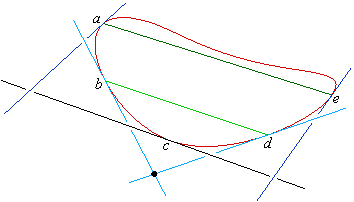
\includegraphics[height=1.5in]{main/cradle-good}
\caption{The lines $bd$ and $ae$ are stationary secants to a degree
  four space curve in red, because the tangents at $b$ and $d$
  have a nonempty intersection, as do (at infinity) the tangents at
  $a$ and $e$.}
\label{Fig9.1}
\end{figure}

More formally we define two subsets of the symmetric square $C_2$ of $C$:
\index{mulsec|defi}%
\index{stat|defi}%
$$
\begin{aligned}
 \mult(C) &\colonequals \{@(p,q) \in C_2 \mid \overlw20{pq} \hbox{ meets
 $C$ in a scheme of length $\geq 3$}@\},\\
\stat(C) &\colonequals  \{@(p,q) \in C_2\setminus \Delta \mid  \hbox{the
tangent lines to $C$ at $p,q$ meet}
@\}.
\end{aligned}
$$
Here
$\overlw20{pq}$
denotes the secant line through $p,q$ (or the
tangent line if $p=q$) and $\Delta\subset C_2$
is the diagonal.


Clearly if $C$ is strange or planar then $\stat(C) = C_2\setminus \Delta$,
and
if $C$ is
planar with $\deg C>2$ then $\mult(C) = C_2$.
These are the only such cases:

\begin{proposition}\label{mult and stat}
 If $C\subset \PP^r$ is a reduced, irreducible, curve that is neither
 planar nor strange, then $\mult(C)\subset C_2$
 and $\stat(C)\subset C_2\setminus \Delta$ are closed subsets of dimension
at most
 $1$.
\unif
\end{proposition}

\begin{proof}
To show that $\mult(C)$ is closed, consider the projection map
$$
\{((p,q), r) \in C_2\times \PP^r \mid r \in \overlw20{pq}@\} \to C_2
$$
sending  $((p,q),r)$ to $(p,q)$. By the
semicontinuity of the degree
\index{semicontinuity of degree}%
in proper families of constant fiber dimension, the set of points lying
in fibers
of length $\geq 3$ is closed, and $\mult(C)$ is the image of this
set. Because the map is finite,
$\mult(C)$  is closed as well.

Similarly, since
$
\{((p,q), r) \in (C_2\setminus \Delta)\times \PP^r \mid r \in {\mathbb T}_p(C)\cup
{\mathbb T}_q(C) \}
$
is closed in $(C_2\setminus \Delta)\times \PP^r` `$, its image under
the projection to the first factor,
which is $\stat(C)$, is closed in $C_2\setminus \Delta$.

Suppose, contrary to the proposition, that $\dim \stat(C) >1$. Since
$\stat(C)$ is a closed subset of the irreducible variety $C_2\setminus
\Delta$ it
follows that $\stat(C) = C_2\setminus \Delta$, so every pair of tangent
lines meet. Any three
lines in projective space that meet pairwise must be either coplanar or
meet in a point. Thus if $C$ is not strange,
then all the tangents to $C$ lie in a common plane, and $C$ is planar,
contradicting our hypothesis
and proving that $\dim \stat(C)\leq 1$.

Finally suppose, contrary to the proposition,  that $\dim \mult(C)>1$. As
in the previous argument, this
implies that every secant is a multisecant.  We will show in this case
that $\dim \stat(C) =2$, a contradiction.

To this end, consider the projections $\pi_{p}: C \to \PP^{r-1}$ and
the set
$$
\tabcolsep1pt
I = \Bigl\{(p,r,r') \in C^3 \Bigm|
\begin{tabular}{l}\small $p,r,r'$ are distinct and\\[-2pt]
\small $\pi_{p}(r) = \pi_{p}(r')$ is a smooth point of $\pi_p(C)$
\end{tabular}
\Bigr\}.
$$
The tangent lines ${\mathbb T}_r(C)$ and ${\mathbb T}_{r'}(C)$ both project from $p$ to the
tangent line ${\mathbb T}_{\pi_p(r)}(\pi_C)$,
and thus they lie in the 2-plane spanned by $p$ and this line; it follows
that $(r,r') \in \stat(C)$.
The projection $I \to C_2: (p,r,r') \mapsto (r,r')$ is finite since the
secant line $\overkern10{rr'}$ meets $C$ in only finitely many points,
so $\dim I \leq \dim \stat(C)$.

 If the projection from some point $p$ were everywhere ramified,
then all tangents to $C$ would pass through $p$, and $C$ would be strange.
Since also every secant to $C$ is a multisecant it follows that  for
every smooth point $p\in C$ there is an open set of points $q\in \pi_p(C)$
such that
the fiber $\pi_p^{-1}(q)$ contains two distinct points of $C$. Thus the
projection $I \to C: (p,r,r') \mapsto p$ maps
$I$ onto an open set of $C$, with 1-dimensional fibers, so $2 = \dim
I\leq \dim \stat(C)$ as claimed.
\end{proof}


\begin{proof}[Proof of Theorem~\ref{linear general position}]
If
$C\subset \PP^n$ is a reduced curve then, by Bertini's theorem, a general
\index{Bertini's theorem}%
hyperplane meets $C$ transversely.
First suppose that $n=3$, and consider the incidence correspondence
$$
I \colonequals  \{ ((p,q), H) \in \mult(C) \times (\PP^3)^* \mid
\overlw20{pq}\in H\}.
$$
Since $\dim \overlw20{pq} = 1$, the fibers of the projection of $I$
to $\mult(C)$ have dimension 1,
so $\dim I = 1+\dim \mult(C)  \leq 2$. Consequently the image of  the
projection of $I$ to $(\PP^3)^*$ has
dimension $\leq 2$, so there is an open set of planes that contain no
multisecants, proving the theorem in this case.

\begin{fact}
 Since a secant line to a curve $C$ that is not itself a line is
 determined by its intersections with $C$,
 every curve other than a line has a 2-parameter family of secant
 lines. If $C\subset \PP^3$ is nondegenerate,
 this means that it is 2 conditions for a line in $\PP^3$ to be a secant
 to $C$. Since a pencil of lines meets
 $C$ in codimension 1, one might expect that, correspondingly, there
 would be a 1-parameter family
 of trisecant lines and a finite number of 4-secant lines. One can
 compute the expected number enumeratively
 \cite[p.~296]{Griffiths-Harris1978}.
 For example a general curve of degree $\leq 4$ can have no 4-secant
 line (it would meet planes containing that line in at least 5 points),
 but a general rational curve of degree 5 in $\PP^3$
  has exactly 1 \cite[Section 12.4.4]{3264}. See  Figure~\ref{9.2}
  for a construction in which the 4-secant line is visible.

\begin{figure}[b]
\centerline {\includegraphics[height=1.5in]{"main/Fig09-2"}}
\caption{A smooth rational quintic in $\PP^{3}$ with a unique 4-fold
secant line
can be obtained as the image of a plane conic $C$ by the rational map
of $\PP^{2}$ to $\PP^{3}$
induced by the 4 cubics through 6 points $e_{1},\dots e_{6}$, exactly
one of which lies on $C$; the image of the unique conic $D$ through the
other 5 points becomes the 4-secant line to the image of $C$.
}
\label{9.2}
\end{figure}

 This fact entered history in a peculiar way:
 After Kronecker \citeyear{Kronecker} proved that every algebraic set in
  $\PP^{n}$ is set-theoretically the intersection of $n+1$
\index{Vahlen @Vahlen, Karl Theodor}%
\index{Kronecker @Kronecker, Leopold}%
\index{set-theoretic equality}%
\index{quintic!rational}%
  hypersurfaces,
Vahlen \citeyear{Vahlen} claimed that Kronecker's result was
  sharp ``because'' a general
rational quintic
\index{historical context}%
with one 4-secant line
  could not be the intersection of 3 hypersurfaces.
  Vahlen played a role in the rise of the Nazi party, and perhaps for
  that reason
Perron \citeyear{Perron} produced 3 hypersurfaces intersecting
\index{Perron @Perron, Oskar}%
  precisely in a given general rational quintic. It is now known that
  every algebraic set in
  $\PP^{n}$ over an infinite field can be written set-theoretically as
  the intersection of just $n$ hypersurfaces \cite{Eisenbud-Evans}.
\end{fact}

We next do induction on $n\geq 4$. We will show first that the image
$C'$ of
$C$ under the projection $\pi_p: C\to C'$ from a general point of $C$
is not strange. Since $C\subset \PP^r$ is neither
planar nor strange
Proposition~\ref{mult and stat} shows that we may choose two smooth points
$r,r'\in C\subset \PP^r$ such that ${\mathbb T}_r(C)\cap {\mathbb T}_{r'}(C) = \emptyset$,
and thus
${\mathbb T}_r(C)$ and ${\mathbb T}_{r'}(C)$ together span a 3-plane $L$. Since $C$ is
nondegenerate we may
choose a point $p\in C$ outside $L$, and it follows that $\pi_p$
restricted to $L$ is an isomorphism.
Thus ${\mathbb T}_{\pi_p(r)}(C') \cap {\mathbb T}_{\pi_p({r'})}(C') = \emptyset$, so $C'$
is not strange,
and since $n\geq 4$ the curve $C'$ is not planar either.

Arguing by contradiction, suppose that the general hyperplane section
of~$C$ contains a set of $r$ linearly dependent points. Consider the
closed subsets
$$
I_1 \subset I \subset \{@(p,H) \in C \times (\PP^n)^*@\}
,
$$
where $I$ is defined by the
condition
that $p\in H$ and $I_1$ is defined
by the condition that, in addition, there exist $p_2,\dots, p_r\in H$
such that $p, p_2, \dots, p_r$ are dependent. Both $I_1$ and $I$ are
closed subsets.

By hypothesis, both $I_1$ and $I$ project onto open sets of $(\PP^n)^*$,
so they have the same dimension.
But $I$ is irreducible: it projects onto an open subset of $C$ with
fibers isomorphic to $\PP^{r-1}$. Thus $I_1 = I$,
and  $p$ is part of a dependent set
$\{p, p_2,\dots, p_r\}$ in a general hyperplane containing $p$.

Let $H'$ be a general hyperplane in $\PP^{n-1}$
and let $H = \pi_p^{-1}(H')$, which is a general hyperplane containing
$p$. The intersection $H\cap C$
contains $r$ dependent points $\{p, p_2,\dots, p_r\}$, and it follows
that $\pi_p(p_2),\dots,\pi_p(p_n)$
are dependent points of $H'\cap C'$. This contradicts the induction
hypothesis, and proves that
the general hyperplane section of $C$ is in linearly general position.
\end{proof}

 \section{Castelnuovo's theorem}\label{CastelnuovoSection}

Clifford's theorem gives a complete and sharp answer to the question,
\index{Castelnuovo's theorem}%
``what linear series can exist on a curve of genus $g$?''
But maybe that wasn't the question we meant to ask! After all, we're
interested in describing curves in projective space as images of abstract
curves $C$ under maps given by linear seriess on $C$. Observing that
the linear series that achieve equality in
Clifford's theorem
\index{Clifford's theorem}%
give maps of degree 2 onto a rational curve,
 we might hope that we
would have a
 different and more relevant
answer if we
restrict our attention to linear series $\cD = (\cL,V)$ for which the
\index{birational}%
associated map $\phi_\cD$ is at least  birational onto its image.

A classical result of Castelnuovo does exactly that: it gives a sharp
bound on the
arithmetic genus
\index{arithmetic genus}%
of a reduced, irreducible, nondegenerate
curve of degree $d$ in $\PP^r` `$. To state it, for positive integers $d$
and $r$, let
\index{M@$M=M(d,r)$|defi}%
\label{def of M}
$$
 M \colonequals
M(d,r)
\colonequals
\biggl\lfloor\mfrac{d-1}{r-1}\biggr\rfloor,
$$
so that
$$
 d -1 = M(r-1) + \epsilon
$$
for some $\epsilon =
\epsilon(d,r)
$
 with $0 \leq \epsilon \leq r-2$.
\index{epsilon@$\epsilon=\epsilon(d,r)$|defi}%

\begin{theorem}[Castelnuovo bound]\label{Castelnuovo's bound}
Let $C \subset \PP^r$ be a reduced, irreducible, nondegenerate curve of
\index{Castelnuovo bound}%
degree $d$. With $M$ and $\epsilon$ defined
as above,
$$
p_a(C) \leq \pi(d,r) \colonequals  \frac{M(M-1)}{2}(r-1) + M\epsilon.
$$
Moreover, if $p_a(C) = \pi(d,r)$  then $C$ is arithmetically
\index{ACM}%
Cohen--Macaulay and every hyperplane
section $H\cap C$ has
Hilbert function
\index{Hilbert function}%
$
\dim (R_{H\cap C})_{m} = \min\{m(r-1), d\}.
$
\end{theorem}

We will say that a curve achieving the bound is a \emph{Castelnuovo
\index{Castelnuovo curve}%
curve}.

\subsection*{Proof of Castelnuovo's bound}

The idea of Castelnuovo's proof is simple and beautiful. To start
with, the hypothesis that $C$ is nondegenerate in $\PP^r$ says that
$h^0(\cO_C(1)) \geq r+1$. We'd like to use this and the Riemann--Roch
formula, in the form
$$
g = d+1 - h^0(\cO_C(1)) + h^1(\cO_C(1)),
$$
but this doesn't work because we have a priori no way to estimate
$h^1(\cO_C(1))$.

Castelnuovo's solution  is to derive lower bounds not just on
$h^0(\cO_C(1))$ but on $h^0(\cO_C(m))$ for all $m$; since we know that
$h^1(\cO_C(m)) = 0$ for large $m$, a lower bound on $h^0(\cO_C(m))$
for large $m$ will translate directly into an upper bound on~$g$.

How can we go about estimating $h^0(\cO_C(m))$? The answer is to
derive lower bounds on the successive differences $h^0(\cO_C(m)) -
h^0(\cO_C(m-1))$, by letting $\Gamma = C \cap H$ be a general hyperplane
section of $C$, and viewing $H^0(\cO_C(m-1))$ as the subspace of
$H^0(\cO_C(m))$ consisting of sections vanishing on $\Gamma$. The
estimates we get may seem crude\emdash not surprisingly, considering
how little we know about~$\Gamma$\emdash but remarkably, the bound we
ultimately derive on the genus of $C$ turns out to be sharp!

For the proof, the following definition will be convenient:

\begin{definition}
If $\sV = (V,\cL)$ is a linear series on a variety $X$ and $\Gamma$
is a subscheme then the \emph{number of conditions imposed by $\Gamma$
\index{number of conditions!imposed by subscheme on a linear series}%
on $\sV$} (that is, the number of
independent linear conditions
\index{independent linear conditions}%
for a
section in $V$ to vanish
identically on $\Gamma$) is the dimension of the image of $V$ in
$H^0(\sL|_\Gamma) = H^0(\sL \otimes \sO_\Gamma)$; or, numerically,
$$
\dim V - \dim \left(V \cap H^0(\cL\otimes \cI_{\Gamma/X}) \right).
$$
\end{definition}

Thus, for example, if $\Gamma \subset \PP^r` `$, then the number of
conditions imposed by $\Gamma$ on $H^0(\cO_{\PP^r}(m))$ is the value
$h_\Gamma(m)$ of the Hilbert function of $\Gamma$ at $m$.
Note that in case $\Gamma$ is zero-dimensional, the number of conditions
imposed by $\Gamma$ on a linear series $V$ is necessarily less than or
equal to the degree $d$ of $\Gamma$; if it is equal we say that $\Gamma$
\emph{imposes independent conditions on $V$}.

\begin{proof}[Proof of Theorem~\ref{Castelnuovo's bound}]
Suppose that $C \subset \PP^r$ is an irreducible, nondegenerate curve. For
large $m$ we have
$h^{0}(\sO_{C}(m)) = md-p_{a}(C) +1$, so to bound the genus from above
we must
bound $h^{0}(\sO_{C}(m))$ from below.

Let $\Gamma = C@\cap@H$ be a general hyperplane section of $C$, and
let $V_m`\subset`H^0(\cO_C(m))$ be the linear series cut on $C$ by
hypersurfaces of degree $m$ in $\PP^r` `$, that is, the image of the
restriction map
$$
H^0(\cO_{\PP^r}(m)) \to H^0(\cO_C(m)).
$$
The number of  conditions imposed by $\Gamma$ on $V_m$ is the rank of
the restriction map
$\rho_m: V_m \to \sO_\Gamma(m)$.
 The number of conditions imposed by $\Gamma$ on $H^{0}(\sO_{C}(m))$
 is the
 rank of the restriction map from this potentially larger space, and
 thus is at least as large. This
 accounts for the inequality in the following:
{\advance\jot-2pt
\begin{align*}
h^0(\cO_C(m)) - h^0(\cO_C(m-1)) & = \text{\# of conditions imposed by
$\Gamma$ on $H^0(\cO_C(m))$}\\
&\geq \text{\# of conditions imposed by $\Gamma$ on $V_m$} \\
&= \text{\# of conditions imposed by $\Gamma$ on $H^0(\cO_{\PP^r}(m))$} \\
&= h_\Gamma(m).
\end{align*}}%
Replacing $m$ by $k$ in the display above and summing
over $k$, we obtain the lower bound
$$
h^0(\cO_C(m)) \geq \sum_{k=0}^m h_\Gamma(k).
$$

In order to bound the genus $C$ from above, we will bound the Hilbert
function of its hyperplane section $\Gamma$  from below; and for this,
we need to know something about the geometry of $\Gamma$. In fact, all
we need to know is Theorem~\ref{linear general position}, which says
that the points of $\Gamma$ are in
linearly general position!
\index{linearly general position}%

\begin{proposition}\label{min hilb}
If $\Gamma \subset \PP^r$ is a collection of $d$ points in linearly
general position that span $\PP^r` `$, then
$$
h_\Gamma(m) \geq
@
\begin{tcases}
mr+1&\hbox{ if $m\leq M(d,r+1)$,}\\
\hfil d &\hbox{ otherwise.}
\end{tcases}
$$
\end{proposition}

One way to understand the bound $mr+1$ is to realize that if $\Gamma$
is any finite subscheme of a rational normal curve $C\subset\PP^r$
of degree $r$,
then $h_\Gamma(m) = \min\{\deg \Gamma,@ mr`+`1\}$ for every $m$
(Exercise~\ref{linear bound is sharp}).
  Thus the bound in Proposition~\ref{min hilb} is best possible.
On the other hand, sets of points on a rational normal curve are almost
the only sets for which the bound is sharp. See Figure~\ref{Fig9.3}
for an illustration.

\begin{figure}
\centerline {\includegraphics[height=1.5in]{"main/Fig09-3"}}
\caption{The case $d = 3\cdot 2+1$: the point $e_{7}$ imposes an additional
condition on the cubics (such as the union of the three lines shown)
passing through
$e_{1},\dots, e_{6}$.}
\label{Fig9.3}
\end{figure}

\begin{proof}
Suppose first that $d \geq mr+1$, and let $p_1,\dots,p_{mr+1} \in
\Gamma$ be any subset of $mr+1$ points. It suffices to show that
$\Gamma' = \{p_1,\dots,p_{mr+1}\}$ imposes independent conditions
on
$H^0(\cO_{\PP^r}(m))$, that is, for any $p_i \in \Gamma'$ there is a
hypersurface $X \subset \PP^r$ of degree $m$ containing all the points
$p_1,\dots, \hat{p_i},\dots,p_{mr+1}$ but not containing~$p_i$.

To construct such an $X$, group the $mr$ points of $\Gamma' \setminus
\{p_i\}$ into $m$ subsets $\Gamma_k$ of cardinality $r$; each set
$\Gamma_k$ will span a hyperplane $H_k \subset \PP^r` `$, and we can
take $X = H_1 \cup \dots \cup H_m$.

In the case where $d<mr+1$, we add $mr+1-d$ general points; each one
imposes exactly one
additional condition on hypersurfaces of degree $m$.
\end{proof}


To complete the proof of Theorem~\ref{Castelnuovo's bound} we add up the
lower bounds in the proposition. To this end, let $C \subset \PP^r$ be
 an irreducible, nondegenerate curve of degree $d$, and  set
$M= M(d,r) = \bigl\lfloor{\frac{d-1}{r-1}}\bigr\rfloor$
as on page~\pageref{def of M}.
We have
\begin{align*}
h^0(\cO_C(M)) &= \sum_{k=0}^M h^0(\cO_C(k)) - h^0(\cO_C(k-1)) \\
&\geq  \sum_{k=0}^M (k(r-1)+1)
= \frac{M(M+1)}{2}(r-1) + M + 1
,
\end{align*}
and similarly
$$
h^0(\cO_C(M+m)) \geq \frac{M(M+1)}{2}(r-1) + M  + md+ 1
.
$$
For sufficiently large $m$, the line bundle $\cO_C(M+m)$ is nonspecial,
so by the
Riemann--Roch theorem,
\index{Riemann--Roch theorem}%
\begin{align*}
g &= (M+m)d - h^0(\cO_C(M+m)) + 1 \\
&\leq (M+m)d - \left(  \frac{M(M+1)}{2}(r-1) + M + 1 + md \right)+1 \\
& = M\bigl( M(r-1) + 1 + \epsilon \bigr) - \left(  \frac{M(M+1)}{2}(r-1)
+ M  \right) \\
&= \frac{M(M-1)}{2}(r-1) + M\epsilon.
\end{align*}


In the case of equality, to show that $C$ is arithmetically
Cohen--Macaulay we must show that $V_{m} = H^0(\cO_C(m))$ for all $m$.
Consider the diagram
\vspace*{3pt}
$$
\small
\xymatrix{
0\ar[r]& 
H^{0}(\sO_{\PP^{r}}(m-1))\ar[r]\ar[d]^{\mathrm{ surjection}}&
H^{0}(\sO_{\PP^{r}}(m))\ar[r]\ar[d]^{\mathrm{ surjection}}&
H^{0}(\sO_{\Gamma}(m))\ar[d]^{=} \\
0\ar[r]& V_{m-1}\ar[r]\ar[d]^{\mathrm{ injection}}&
V_{m}\ar[r]\ar[d]^{\mathrm{ injection}} &
H^{0}(\sO_{\Gamma}(m))\ar[d]^{=} \\
0\ar[r]& H^{0}(\sO_C(m-1))\ar[r]&H^{0}(\sO_C(m))\ar[r] &H^{0}(\sO_{\Gamma}(m))
\rlap{.}
}
\vspace*{3pt}
$$
The top and bottom rows are left exact. From the left exactness of the
bottom row
it follows that the map $V_{m-1}\to V_{m}$ is an injection. From
the left exactness of the
top row it follows that this map is the kernel of the restriction map
$V_{m} \to H^{0}(\sO_{\Gamma}(m))$.
Thus the middle row is also left exact, and we see that the number of
conditions that
$\Gamma$ imposes on $V_{m}$ is equal to $\dim V_{m}-\dim V_{m-1}$.

From the first part of the proof we have inequalities
$$
\displaylines{
 \text{\# of conditions imposed by $\Gamma$ on $H^{0}(\sO_C(m))$}
\hfill\cr\hfill
\geq
\text{\# of conditions imposed by $\Gamma$ on $V_{m}$},
}
$$
that is,
$$
h^0(\cO_C(m)) - h^0(\cO_C(m-1))\geq \dim V_{m}-\dim V_{m-1}
.
$$
If $g = \pi(d,r)$ then these must both be equalities. Thus
for large $m$ the restriction map
$H^{0}(\sO_{\PP^{r}}(m)) \to H^{0}(\sO_{C}(m))$ is surjective, so
\jot=-5pt % mesh sums; scoped by end of proof
\begin{align*}
\sum_{k=0}^m (h^0(\cO_C(k)) - h^0(\cO_C(k-1))
&= h^0(\cO_C(m)) = \dim V_m \\
&= \sum_{k=0}^m (\dim \Vk - \dim \Vkmi).
\end{align*}
However, for each $k$ we have
$$
\dim \Vk - \dim \Vkmi\geq h^0(\cO_C(k)) - h^0(\cO_C(k-1)),
$$
and thus we must have equality for all $k$, whence  $\dim
\Vk
=h^0(\cO_C(k))$ for all $k$; that is, $C$ is arithmetically
\index{ACM}%
Cohen--Macaulay.

Always supposing that  $p_{a}(C) = \pi(d,r)$, the inequalities in
Proposition~\ref{min hilb}
must be equalities, so for a general hyperplane section $\Gamma = H\cap C$
we have $h_{\Gamma}(m) = \min \{m(r-1)+1, d\}$ for all $m\geq 0$. However,
since
$C$ is arithmetically Cohen--Macaulay, $h_{\Gamma}(m) = h^{0}(\sO_{C}(m))
- h^{0}(\sO_{C}(m-1)) $
for every hyperplane section $\Gamma$, completing the proof.
\end{proof}

 \subsection*{Consequences and special cases}

 First of all,
if
$r=2$ we have $\pi(d,r) = \tbinom{d-1}{2}$,
 so every
plane curve
(smooth or not)
is a Castelnuovo curve.
\index{plane curve!is a Castelnuovo curve}%

 In case $r=3$, we have
 $$
 \pi(d,r) =
 \begin{cases}
 \left(\frac{d-2}{2} \right)^2& \quad \text{if $d$ is even}, \\
\noalign{\vskip3pt}
 \left(\frac{d-1}{2} \right)\left(\frac{d-3}{2} \right)& \quad \text{if
 $d$ is odd},
 \end{cases}
 $$
 which we can recognize as the genus of curves of type $(\unfrac{d}{2},
 \unfrac{d}{2} )$ on a quadric surface in case $d$ is even, and the genus
 of curves of type
 $\bigl(\upnfrac{d{+}1}{2}, \upnfrac{d{-}1}{2} \bigr)$
on a quadric when $d$ is odd. Thus
the Castelnuovo bound is sharp when $r=3$ as well.

Indeed, the Castelnuovo bound is sharp for all $d$ and $r$; we'll
prove this, and describe explicitly the curves that achieve it, in
Chapter~\ref{ScrollsChapter}.


\begin{corollary}\label{list of Castelnuovo curves}
Suppose that $C\subset \PP^r$ is a smooth curve of arithmetic genus
$p_{a}$ and degree $d$ embedded by a complete linear series. The curve
$C$ is  Castelnuovo (and thus arithmetically Cohen--Macaulay) if and
only~if one of the following
conditions
holds:
\begin{enumerate}
\item  $d<2r$ and  $d \geq 2p_a+1$.
\item $d=2r$
and
$C$ is a canonical curve.
\item $r=3$, $d>6$,
and
$C$ is a divisor on a (smooth or singular)
irreducible quadric in the class $mH$ or $mH+L$, where $H$ is the class
of a hyperplane and $L$ is the class of a line.
\item  More generally,  $d>2r$
and
$C$ lies on a rational normal scroll in a certain range of divisor classes
\rm
(Theorem~\ref{Castelnuovo examples}).
\end{enumerate}
\end{corollary}

\begin{fact}
Corollary~\ref{list of Castelnuovo curves} remains true with appropriate
definitions also for reduced irreducible curves. This can be proven
with the techniques developed in Chapters~\ref{LinkageChapter}
and~\ref{ScrollsChapter}.
\end{fact}

\begin{proof}
Simple arithmetic shows that if $d\geq 2p_a+1$  then  $d<2r$ and $p_a=
\pi(d,r)$. Moreover if $p_a= \pi(d,r)$ and $d<2r$,
then indeed $d\geq 2p_a+1$, proving~
(1).

If $d= 2r$ then $\pi(d,r) = r+1$, and Clifford's theorem shows that $C$
is a canonical curve, proving
(2).

Now suppose that $r=3, d>6$ and let $\Gamma$ be a hyperplane
section of $C$. Since $h_{\Gamma}(2) = \min\{2\cdot 2+1,@ d\} = 5$,
$\Gamma$
lies on a conic, and
since $C$ is arithmetically Cohen--Macaulay, $C$ must lie on a quadric.
If $C$ is smooth then arithmetic plus the result of Section~\ref{Div of
quadric} establishes the
claim.
For the more general case (4),
and the case $r>3$, see Theorem~\ref{Castelnuovo examples}
in Chapter~\ref{ScrollsChapter}, where we define rational normal scrolls.
\end{proof}

The most important special case is that of canonical curves:

\begin{corollary}\label{canonical hilbert function}
If $C\subset \PP^{g-1}$ is a canonical curve then the Hilbert function
\index{canonical curve}%
\index{Hilbert function}%
\index{homogeneous coordinate ring}%
of the homogeneous coordinate ring $S_{C}$ of  $C$ depends only on $g$,
and is given by
\smallskip %FMT
$$
\dim({S_{C}})_{n} = h^{0}(\cO_{C}(n)) =
\begin{tcases}
 \hfil 0 & \mbox {if } @d<0,\\
 \hfil 1 & \mbox {if } @d=0,\\
 \hfil g & \mbox {if } @d=1,\\
 @(2g{-}2)n + 1 - g & \mbox {if } @d>1.\\
\end{tcases}
$$
\end{corollary}

\begin{proof}
Theorem~\ref{Castelnuovo's bound} implies that the homogeneous coordinate
ring of $C$ can be identified with $\bigoplus_{n\in \ZZ}\HH^0(\sO_C(n))$,
and the dimensions of these spaces are determined by the Riemann--Roch
theorem.
\end{proof}


\begin{fact}
A famous theorem of Gruson and Peskine \citeyear{MR0690647} (see
\index{Gruson @Gruson, Laurent}%
\index{Peskine @Peskine, Christian}%
\cite{MR0689536} for an exposition and also the case of
positive
characteristic) completes the picture of the
possibilities for the degree $d$ and  genus $g$  of a smooth curve in
$\PP^3` `$. If the curve does not lie on a plane or a quadric, then the
genus satisfies the stronger inequality
$$
g\leq
\pi_1(d,3)
\colonequals  \frac{d^2-3d}{6} +1
$$
and smooth curves with all such degree and genus exist; they can all be
\index{pi@$\pi_1(d,3)$}%
realized as curves
on cubic or quartic surfaces.

Note that there can be gaps in the possible genera of curves a given
degree: for example  $\pi_1(9,3) = 10<\pi(9,3) =12$ but there is
no curve of degree 9 and genus 11.
The full range of possible degrees and genera for curves in $\PP^r$
remains open for larger $r$.
See
\cite{MR0589222} for a summary and a number of
conjectures.
\end{fact}


\section{Other applications of linearly general position}
\label{projection section}\label{good projections}

\subsection*{Existence of good projections}

We can use Theorem~\ref{basic linear independence} to show that every
\index{good projection}%
smooth curve $C$ is
birational
\index{birational!nodal plane curve}%
\index{nodal plane curve}%
to a
nodal plane curve
$C_0 \subset \PP^2``$, in many ways.

\begin{proposition}\label{nodal projection}
If $C \subset \PP^n$ is a smooth nondegenerate curve in projective space,
let $\Lambda \cong \PP^{k} \subset \PP^n$ be a general $k$-plane, and let
$\pi_\Lambda : C \to \PP^{n-k-1}$ be the projection from $\Lambda@$,
restricted to $C$. If  $n-k-1 \geq 3$
then
$\pi_\Lambda: C \to \PP^{n-k-1}$ defines an isomorphism of $C$ onto
its image, while if $n-k-1 = 2$ then $\pi_\Lambda$
is birational onto its image, which is a curve with only nodes.
\end{proposition}

\begin{proof} Recall that the
secant variety
\index{secant variety}%
of $C$ consists of the
union of the lines $\overlw20{qr}$ joining pairs of distinct points
$q,r \in C$, plus the tangent lines ${\mathbb T}_q(C)$; altogether,
these lines form a family, parametrized by the symmetric square $C_2$
of $C$. More precisely every subscheme $\lambda$ of
length 2 in $\PP^n$ spans a line $\overline \lambda$. The incidence
variety
$$
I\colonequals \bigl\{(\lambda, p)\mid \lambda\in C_2 \hbox{ is a divisor of
degree 2 on }C,\ p\in \overline \lambda\subset\PP^n\bigr\}
$$
projects to $C_2$ with 1-dimensional fibers isomorphic to $\PP^1` `$,
and thus
is irreducible of dimension 3. Its image in $\PP^n$ under the second
projection
is the secant variety of $C$, which is thus irreducible of dimension
$\leq 3$.
It follows that a general
$(n-4)$-plane does not meet the secant variety, and the first statement
of the proposition follows.

If $n>3$ then by first projecting from a general $(n-4)$-plane inside
$\Lambda$ we may reduce to the case $n=3$, and assume that $\Lambda$ is a
general point of $\PP^3` `$. By a variant of the argument above, the union
of the tangent lines to $C$ is a surface, and thus does not contain
$\Lambda$.
It follows that $\pi_\Lambda$ is locally in the source an analytic
isomorphism.

To show that the fibers of $\pi_\Lambda$ are subschemes of length at
most 2,
we need to show that $\Lambda$ does not lie on any
\index{multisecant line}%
multisecant line.

By Theorem~\ref{basic linear independence} the family of multisecant
lines to $C$ is a proper subscheme of the irreducible two-dimensional
family of secant lines, so the union of the trisecant lines is at most 2
dimensional, and we see that the fibers of $\pi_\Lambda$ all have degree
$\leq 2$. Furthermore, the general fiber of the projection
from the incidence correspondence $I$ to $\PP^3$ is empty or finite,
so only a finite number of secant lines contain $\Lambda$, and we see
that $\pi_\Lambda$ is birational.

We have shown that the map $\pi_\Lambda$ is an immersion, and at
most two-to-one everywhere; thus the image curve $C_0 \subset \PP^2$
has at most double points, and an analytic neighborhood of each
double point  consists of two smooth branches. To complete the proof
of Proposition~\ref{nodal projection} we have to show that those two
branches have distinct tangent lines; that is, that
if $q, r \in C$ are any two points collinear with $\Lambda$, then the
images of the tangent lines ${\mathbb T}_q(C)$ and ${\mathbb T}_r(C)$ in
$\PP^2$ are distinct. But if  $\pi_p({\mathbb T}_q(C)) = \pi_p({\mathbb
T}_r(C))$ then  ${\mathbb T}_q(C)$ and ${\mathbb T}_r(C)$ lie in a plane,
and thus intersect.

Since the family of all secant lines is irreducible of dimension 2,  it
will suffice to show that not every secant line to $C$ is a
stationary secant
\index{stationary secant}%
or, equivalently, that not every pair of tangent lines to $C$
meet. We saw in Proposition~\ref{mult and stat} that in the contrary
case
$C$ would be either strange or planar, a contradiction.
\end{proof}


\subsection*{The case of equality in Martens' theorem}

We can now revisit
the case
of equality in
\index{Martens' theorem}%
Martens' theorem
bounding the dimension of the variety
$W^r_d(C)$
\index{W@$W^r_d$}%
that parametrizes
divisor classes of degree $d$ on a curve $C$
with $r(D) \geq\nobreak r$
(Theorem~\ref{Martens' inequality}).
To start, recall the statement:

\begin{theorem}[Martens]\label{full Martens}
If $C$ is any smooth projective curve of genus $g$, then for any $r>d-g$
we have
$$
\dim W^r_d(C) \leq d-2r.
$$
Equality holds if and only~if either $C$ is
hyperelliptic
\index{hyperelliptic}%
or $d=r=0$ or $d=2g-2$, $r=g-1$; in either of the last two cases $W^r_d$ is
a single point.
\unif
\end{theorem}

Note that the inequality $\dim W^r_d(C) \leq d-2r$ is equivalent to the
\index{C@$C^r_d$}%
inequality $\dim
C^r_d
\leq d-r$, which is what we actually showed
in Chapter~\ref{new Jacobians chapter}. There we combined
the geometric Riemann--Roch theorem
\index{Riemann--Roch theorem!geometric}%
with an elementary bound on the
dimension of the variety of secant planes to a curve in projective space.
Theorem~\ref{basic linear independence} allows us to sharpen the elementary bound:

\begin{lemma}[strong secant plane lemma]\label{Strong secant plane lemma}
Let $C \subset \PP^n$ be a smooth, irreducible and nondegenerate curve. If
\index{strong secant plane lemma}%
we denote by $
\Sigma^r_d
\subset C_d$ the locus of effective divisors
\index{sigma@$\Sigma^r_d$|defi}%
$D$ of degree $d$ on $C$ with $\dim \overkern20 D \leq d-r-1$, then for
any $d \leq r$ and $r > 0$,
$$
\dim \Sigma^r_d \leq d-r-1.
$$
\end{lemma}

\begin{proof}
Consider the incidence correspondence
$$
\Gamma \colonequals  \bigl\{@(D, H) \in \Sigma^r_d\times
(\PP^r)^*
\mid \overkern20 D \subset H@\bigr\}.
$$
The curve being nondegenerate, the projection map $\Gamma \to  (\PP^n)^*$
is finite. But the fibers of $\Gamma$ over $\Sigma^r_d$ have dimension
at least $n-d+r$; if we had $\dim \Sigma^r_d \geq d-r$, it would follow
that $\dim \Gamma \geq n$, and hence that the projection map $\Gamma
\to  (\PP^r)^*$ is dominant, contradicting Theorem~\ref{basic
linear independence}.
\end{proof}

\begin{proof}[Proof of the case of equality in Martens theorem]
 Now, if a curve $C$ is nonhyperelliptic, we can apply the
strong secant plane lemma
\index{strong secant plane lemma}%
(Lemma~\ref{Strong secant plane lemma})
 to the
canonical curve.
\index{canonical curve}%
Except for the trivial cases $d=r=0$
 and $d=2g-2, r=g-1$,
 we can apply
the lemma
to conclude that
 $\dim W^r_d(C) \leq d-2r-1$; it follows that if
$\dim W^r_d(C)
 = d-2r$ the curve $C$ in question must be hyperelliptic.
\unif
\end{proof}

Using the case of equality in Martens' theorem, we can analyze equality in
Clifford's theorem:
\index{Clifford's theorem!equality in}%

\begin{corollary}\label{equality in Clifford from Martens}
If $C$ is a smooth curve of genus $g$ and $D$
is
a divisor on $C$
whose degree satisfies $\deg D = 2r(D)\le 2g-2$,
then either $D =0$ or $D=K_C$ or $C$
is hyperelliptic.
\unif
\end{corollary}

\begin{proof}
If $C$ has a divisor $D$ with $\deg D =2 r(D)$ then by the Riemann--Roch
theorem,  $\deg D  = 2(\deg D-g+h^1(D))$,
so $\deg D = 2g-2h^1(D)$. If also $\deg D\leq 2g-2$, then $h^1(D) \geq 1$
and thus $r(D) >\deg D-g$. Since $W^{r(D)}_{\deg D}$ contains $D$
its dimension
is $\geq 0$, and we have a case of equality in Martens' theorem.
\end{proof}


\subsection*{The $g+2$ theorem}
%\label{g+2 section}

Now that we have the strong form of Martens' theorem, we can prove the
analogue of Theorem~\ref{g+3 theorem} for general linear series of degree
$g+2$. This was stated in Section~\ref{g+3 section}, but
we
reproduce
the statement here.
\index{g@$g+2$ theorem|defi}%

\begin{theorem}\label{needed for nodes}
Let $C$ be any smooth projective curve of genus $g$, and let $D$ be a
general divisor of degree $g+2$ on $C$.
The complete linear series $|D|$ is basepoint free of dimension \2,
and the associated map $\phi_D: C\to \PP^2$
 is a
birational
immersion
\index{birational}%
onto its image $C_0$
and no two branches of $C_0$ share a tangent line.
Moreover:

\begin{enumerate}
\item If $C$ is not hyperelliptic, then $C_0$ has only $\tbinom{g}{2}$
nodes and no other singularities.
\item If $C$ is hyperelliptic,
then
$C_0$ has only one singular point,
  which is an ordinary $g$-fold point.
\end{enumerate}
\end{theorem}

Figure~\ref{Fig9.4} illustrates the two possibilities.

\begin{figure}
\leavevmode\raise0.05in\hbox{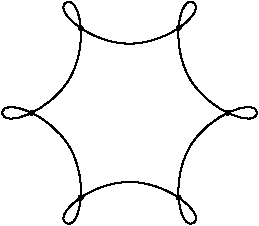
\includegraphics[height=1.1in]{main/Fig09-4A}}
\qquad
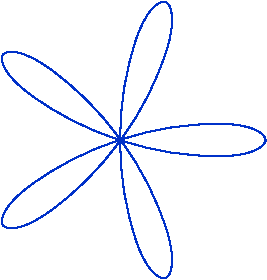
\includegraphics[height=1.2in]{main/five}
\caption{A general linear series of degree $g+2$ maps a nonhyperelliptic
curve of genus $g$
to a plane curve with $\protect\sbinom{g}{2}$ nodes
but the image of a
hyperelliptic curve has
just one singular point, where $g$ smooth branches intersect with
distinct tangents.
}
\label{Fig9.4}
\end{figure}

\begin{proof}
%\begin{itemize}
% \item (Dimension)
Since $D$ is general and $\deg D > h^{0}(K)$ we see
that $D$ is nonspecial, whence $h^0(D) = (g+2)-g+1 = 3$.
This yields the dimension claim.

%\item (no basepoints)
If $|D|$
has
a basepoint $p\in C$, then $3=h^0(D)
= h^0(D-p) = (g+1)-g+1+h^0(K_C-D+p)$,
so $K_C-D$ is effective of degree $2g-2-(g+1) =g-3$; thus the family of
such $D$ depends on only $g-3+1$ parameters,
and $\mu(D)$ would lie in a proper subvariety of $\Pic_{g+2}(C)$,
contradicting generality.

Next we show that
there are only finitely many pairs $p,
q \in C$ such that $\phi_D(p) = \phi_D(q)$; that is, $\phi_D$
is birational onto its image.
Indeed, $\phi_D(p) = \phi_D(q)$
 means that $h^0(D-p-q) = 2$. By the Riemann--Roch
 theorem, $D-p-q = K-E$ for some effective divisor $E$ of degree $g-2$;
 thus $\sO_C(D)$ is in the image of the map
$$
\nu : C_2 \times C_{g-2} \to \Pic_{g+2}(C)
$$
sending $(p+q, E)$ to $K_C - E + p + q$.
But
$\nu$ is
the composition of two surjective maps, $C_2 \times C_{g-2} \to C_g$
and $C_g\to Pic_g \to Pic_{g+2}$ by duality. Since the source and
target of $\nu$ have the same dimension, the general fiber of $\nu$ is
finite.

We turn to the types of singularities. First we eliminate tacnodes.
To say that a pair of points $p, q \in C$ map to
a point of $C_0$ such that the
two branches have a common tangent means two things: that $h^0(D-p-q)
\geq 2$; and that $h^0(D-2p-2q) \geq 1$. If this is the case, set $E =
D - 2p - 2q$.  The condition $h^0(D-2p-2q) \geq 1$ is equivalent to
$E$ being an effective divisor. Considering the canonical map $\phi_K:
C\to \PP^{g-1}$
the
geometric Riemann--Roch theorem,
\index{Riemann--Roch theorem!geometric}%
$$r(E) = \deg E -1-\dim\overlow{\phi_K(E)},$$
implies that $\overlow {\phi_K(E)}$ has
dimension $g-3$. The
further
condition $h^0(D-p-q) \geq 2$ says that
$\dim\overlow{\phi_K(E+p+q)} = g-2$,
so the secant line $\overlw20{pq}$ meets the $(g-3)$-plane
$\overlow{\phi_K(E)}$. Now, not every secant line to $C$ can meet
a given linear subspace $\Lambda \subset \PP^{g-1}$ of dimension
$g-3$\emdash otherwise, the projection $\pi_\Lambda : C \to \PP^1$ would
be constant\emdash so we see that $\mu(D)$ would have to lie on the image
of a proper subvariety of $C_{g-2} \times C_2$ under the map $(E, p+q)
\mapsto \sO(E+2p+2q)$ from $C_{g-2} \times C_2$ to $\Pic_{g+2}(C)$.
Since the dimension of this subvariety is $<g$ we see that if $C'$ has
a point at which two branches are tangent, then $\sO_C(D)$ lies in a
proper subvariety of $\Pic_{g+2}(C)$. Since
the Abel--Jacobi map $C_{g+2} \to Pic_{g+2}(C)$ is surjective,
 $D$ would not be general.

\smallbreak
Now let's suppose that $C$ is nonhyperelliptic.
To prove
claim (1) of the theorem,
we
have to show
that the image $C_0 = \phi_D(C)$
has only nodes as singularities,
rather than cusps or triple points.
That there are exactly
$\tbinom{g}{2}$ nodes then follows from the
adjunction formula.
\index{adjunction formula}%

\begin{itemize}
\item []\hskip-\leftmargini (no cusps)\,
To say that a point $p \in C$ maps to a cusp of $C_0$
(that is, the differential $d\phi_D$ is zero at $p$) amounts to saying
that $h^0(D-2p) \geq 2$; that is, $D-2p$ is a $g^1_g$. But by the
Riemann--Roch theorem, $W^1_g = K_C - W_{g-2}$; so to say $\phi_D$
has a cusp means that
$$
\mu(D) \in 2W_1 + K_C - W_{g-2},
$$
and since the locus on the right has dimension at most $g-1$, a general
point of $J(C)$ will not lie in it. Note that this subsumes the fact
that $|D|$ has no basepoints.

\item []\hskip-\leftmargini (no triple points)\,
To say that $C_0$ has a triple point means
that for some divisor $E = p+q+r$ of degree 3, $h^0(D-E) \geq 1$; thus
we must have
$$
\mu(D) \in W_3^{} + W^1_{g-1}.
$$
To argue that this is not the case, we need to know that $\dim W^1_{g-1}
\leq g-4$;
streamlined
if $C$ is nonhyperelliptic.
\end{itemize}

\noindent This concludes the proof in the nonhyperelliptic case. Now
suppose that $C$ is hyperelliptic, and let $|E|$ be the  $g^1_2$ on
$C$.
Since $D$ is a
divisor of degree $g+2$, the divisor $D - E$ will
have degree $g$, and so be effective; thus we can write
$D \sim E + p_1 + \dots + p_g$
for some
$g$ points $p_i$, which must be distinct since $D$ was assumed general.

The fact that
$$
h^0(D - p_1 - \dots - p_g) = h^0(E) = 2 = h^0(D) - 1
$$
implies that $\phi_D$ maps all the points $p_i$ to the same point. The
image curve $C_0$ thus has a point with at least $g$ branches. Since
these branches cannot share a tangent line,
they are smooth and their tangents are distinct; that is, the point is
an ordinary multiple point. By the adjunction
\index{adjunction formula}%
formula $p_a(C) = \tbinom{g+1}{2}$ and since $C$ has genus $g$ the
singularity must have $\delta$ invariant
$\tbinom{g+1}{2} -g = \tbinom{g}{2}$. Such a singularity cannot have
multiplicity $>g$, and is thus a $g$-fold point. Since the
\index{delta invariant@$\delta$ invariant}%
$\delta$ invariant of such a point is at least $\tbinom{g}{2}$ by
the discussion following Theorem~\ref{divisor classes on blowup}
(see also
Proposition~\ref{effect of blowup on genus}), the $g$-fold point is ordinary and there can be no other
singularities.
\end{proof}

\section{Exercises}

\begin{exercise}
Let $C\subset \PP^r$ be a smooth curve
over an algebraically closed field of arbitrary characteristic.
We can
re-embed $C$ by a
Veronese map,
that is, consider $\widetilde C = \nu_m(C)$ where
$\nu_m :
\PP^r \to \PP^N$ is the $m$-th Veronese map. Prove:

\begin{proposition}[%
compare
~Proposition~\ref{nodal projection}]
\label{positive characteristic nodes}
If $m$ is high enough then
the projection of~$@\widetilde C$ from a general $\PP^{N-3}$
is a birational map onto a nodal
plane curve.
\tohint{10.1}
\end{proposition}
\end{exercise}

\begin{npt}
\begin{exercise}[\cite{Rathmann}]
\label{strange curves} Let $k$ be an
\index{Rathmann, J\"{u}rgen}%
algebraically closed field of characteristic $p>0$, and let $q=p^e$
for some $e\geq 1$. Let $C\subset \PP^r$
be the closure of the image $C_0$ of the morphism
$$
\AA^1 \ni t \mapsto (t, t^q, t^{q^2}, \dots , t^{q^{r}}) \in \AA^r
$$
where $\AA^r\subset \PP^r$ is the open set $x_0=1$.
\begin{enumerate}
\item Show that $C$ is a complete intersection, defined by the equations
$$
x_0^{q-1}x_2 - x_1^q, x_0^{q-1}x_3 - x_2^q,\dots,
x_0^{q-1}x_r - x_{r-1}^q.
$$
\item Show that $C$ is singular unless $q = r = 2$.
\item Show every secant line to $C_0$ contains $q$ points of $C_0$;
more generally, if
$a_1, \dots, a_r$ are linearly independent points of $C_0$, show that
the linear span of
$a_1, \dots, a_r$ contains $q^{(r-1)}$ points of $C_0$.  Compare this
with the configuration of
points in affine $r$-space over a field of $q$ elements.
\end{enumerate}
\end{exercise}
\end{npt}

\begin{exercise}
Here is another approach to the $g+2$ theorem in the hyperelliptic case:
\index{g@$g+2$ theorem}%
Let $C$ be a
hyperelliptic
\index{hyperelliptic}%
curve of genus $g$ and $D$ a general divisor
of degree $g+1$ on $C$; let $|E|$ be the $g^1_2$ on $C$.
Consider the map $\phi : C \to \PP^1 \times \PP^1$ given as the product
of the maps $\phi_D : C \to \PP^1$ and $\phi_E : C \to \PP^1$ given by
the pencils $|D|$ and $|E|$.
\begin{enumerate}
\item Show that $\phi$ embeds the curve $C$ as a curve of bidegree
$(g+1,2)$ on $\PP^1 \times \PP^1` `$.
\item Now embed $\PP^1 \times \PP^1$ into $\PP^3$ as a quadric surface
$Q$; pick a general point $p \in C \subset Q$ and project $C$ from the
point $p$. Show that the image curve $C_0$ is a plane curve of degree
$g+2$ with one ordinary $g$-fold point.
\tohin{10.2}
\end{enumerate}\label{tnih10.2}
\end{exercise}

\begin{exercise}\label{extremal m-ics}
Establish the analogue of Proposition~\ref{rnc on most quadrics}
for hypersurfaces of any degree $m$, that is to say no irreducible,
nondegenerate curve in $\PP^d$ lies on more hypersurfaces of degree $m$
than the
rational normal curve.
\index{rational normal curve}%
To do this, let $C\subset \PP^d$ be any irreducible nondegenerate
curve. Let $\Gamma$ be a general hyperplane section
of $C$, and use the exact sequences
$$
0 \to \cI_{C/\PP^d}(l-1) \to \cI_{C/\PP^d}(l) \to
\cI_{\Gamma/\PP^{d-1}}(l) \to 0.
$$
with $2 \leq l \leq m$ to show that
$$
h^0(\cI_{C/\PP^d}(m)) \leq  \mbinom{d+m}{m} - (md+1)
$$
with equality only~if $C$ is a rational normal curve.
\end{exercise}

\begin{exercise}\label{linear bound is sharp}
Let $D \subset \PP^r$ be a rational normal curve. If $\Gamma \subset D$
is any collection of $d$ points on $D$ (or for that matter any subscheme
of $D$ of degree $d$) then the
Hilbert function
\index{Hilbert function}%
of $\Gamma$ is
$ h_\Gamma(m) = \min\{d, mr+1\} $.
\tohint{10.5}
\end{exercise}

\begin{exercise}
Let $C$ be a reduced irreducible curve with general hyperplane section
$\Gamma$,
and write
$d-1 = M(r-1) +\epsilon$ with $\epsilon<r-1$ as in Castelnuovo's theorem.
Prove that
\begin{enumerate}
\item if $\epsilon > 0$, then $\cO_C(M)$ is nonspecial, but $\cO_C(M-1)$
is special; and
\item if $\epsilon = 0$, then $\cO_C(M-1)$ is nonspecial, but $\cO_C(M-2)$
\index{epsilon@$\epsilon$}%
is special.
\tohin{10.6}
\end{enumerate}\label{tnih10.6}
\end{exercise}

\begin{exercise}\label{castelnuovo unique}
If $C \subset \PP^r$ is a
Castelnuovo curve
\index{Castelnuovo curve}%
of degree $d \geq 2r$,
show that $|D| = |\cO_C(1)|$ is the unique $g^r_d$ on $C$.
\tohint{10.7}
\end{exercise}

\begin{exercise}\label{rarity of Castelnuovo}
We have seen that complete intersections $C = Q \cap S \subset \PP^3$ of a
quadric surface $Q$ and a surface $S$ of degree $k$ achieve Castelnuovo's
bound $g = \pi(2k, 3)$ on the genus of curves of degree $2k$ in $\PP^3``$.
In fact, we will see in Chapter~\ref{ScrollsChapter} that any curve
$C \subset \PP^3$ of degree $2k$ and genus $g = \pi(2k, 3) = (k-1)^2$
is of this form.
\begin{enumerate}
\item Find the dimension of the subvariety $\Gamma \subset M_g$ consisting
of Castelnuovo curves.
\item Find the dimension of the subvariety $H \subset M_g$ of
hyperelliptic curves, and compare this to the result of the first part.
\tohin{10.8}
\end{enumerate}\label{tnih10.8}
\end{exercise}
\endgroup % redef of \mult



%header and footer for separate chapter files

\ifx\whole\undefined
\documentclass[12pt, leqno]{book}
\usepackage{graphicx}
\input style-for-curves.sty
\usepackage{hyperref}
\usepackage{showkeys} %This shows the labels.
%\usepackage{SLAG,msribib,local}
%\usepackage{amsmath,amscd,amsthm,amssymb,amsxtra,latexsym,epsfig,epic,graphics}
%\usepackage[matrix,arrow,curve]{xy}
%\usepackage{graphicx}
%\usepackage{diagrams}
%
%%\usepackage{amsrefs}
%%%%%%%%%%%%%%%%%%%%%%%%%%%%%%%%%%%%%%%%%%
%%\textwidth16cm
%%\textheight20cm
%%\topmargin-2cm
%\oddsidemargin.8cm
%\evensidemargin1cm
%
%%%%%%Definitions
%\input preamble.tex
%\input style-for-curves.sty
%\def\TU{{\bf U}}
%\def\AA{{\mathbb A}}
%\def\BB{{\mathbb B}}
%\def\CC{{\mathbb C}}
%\def\QQ{{\mathbb Q}}
%\def\RR{{\mathbb R}}
%\def\facet{{\bf facet}}
%\def\image{{\rm image}}
%\def\cE{{\cal E}}
%\def\cF{{\cal F}}
%\def\cG{{\cal G}}
%\def\cH{{\cal H}}
%\def\cHom{{{\cal H}om}}
%\def\h{{\rm h}}
% \def\bs{{Boij-S\"oderberg{} }}
%
%\makeatletter
%\def\Ddots{\mathinner{\mkern1mu\raise\p@
%\vbox{\kern7\p@\hbox{.}}\mkern2mu
%\raise4\p@\hbox{.}\mkern2mu\raise7\p@\hbox{.}\mkern1mu}}
%\makeatother

%%
%\pagestyle{myheadings}

%\input style-for-curves.tex
%\documentclass{cambridge7A}
%\usepackage{hatcher_revised} 
%\usepackage{3264}
   
\errorcontextlines=1000
%\usepackage{makeidx}
\let\see\relax
\usepackage{makeidx}
\makeindex
% \index{word} in the doc; \index{variety!algebraic} gives variety, algebraic
% PUT a % after each \index{***}

\overfullrule=5pt
\catcode`\@\active
\def@{\mskip1.5mu} %produce a small space in math with an @

\title{Personalities of Curves}
\author{\copyright David Eisenbud and Joe Harris}
%%\includeonly{%
%0-intro,01-ChowRingDogma,02-FirstExamples,03-Grassmannians,04-GeneralGrassmannians
%,05-VectorBundlesAndChernClasses,06-LinesOnHypersurfaces,07-SingularElementsOfLinearSeries,
%08-ParameterSpaces,
%bib
%}

\date{\today}
%%\date{}
%\title{Curves}
%%{\normalsize ***Preliminary Version***}} 
%\author{David Eisenbud and Joe Harris }
%
%\begin{document}

\begin{document}
\maketitle

\pagenumbering{roman}
\setcounter{page}{5}
%\begin{5}
%\end{5}
\pagenumbering{arabic}
\tableofcontents
\fi



\chapter{Monodromy of Hyperplane Sections}\label{uniform position}

\section{Uniform position and monodromy} \label{uniformSection}
We now return to the situation where the ground field $k$ is algebraically closed of characteristic 0.

The central result of this chapter is the  \emph{uniform position lemma}, which deals with the monodromy group of the points of a general hyperplane section of a curve $C \subset \PP^r$. To define the monodromy group  and prove the  uniform position lemma, we will use the classical topology. An equivalent algebraic definition is described in Cheerful Fact~\ref{Galois equals monodromy} below, but the strong form of uniform position can fail in positive characteristic,
as shown by the examples in Exercise~\ref{strange curves}.

We may describe the monodromy group informally as follows: Suppose that $C \subset \PP^r$ is an irreducible curve of degree $d$ over $\CC$, and $H_0 \subset \PP^r$ a hyperplane transverse to $C$; say $C \cap H_0 = \{p_1,\dots,p_d\}$. As we vary $H_0$ continuously along a real arc $\{H_t\}$, staying within the open subset $U \subset {\PP^r}^*$ of hyperplanes transverse to $C$, we can ``follow" each of the points $p_i(t)$ of intersection of $C$ with the hyperplane $H_t$.

Now imagine that the hyperplanes $H_t$ come back to the original $H_0$ at time $t=1$; that is, we have a continuous family $\{H_t\}_{0 \leq t \leq 1} \subset U$ with $H_1 = H_0$. Each of the points $p_i$ then traces out a continuous real arc 
$\{p_i(t) \in C \cap H_t\}_{0 \leq t \leq 1}$. Since $H_1 = H_0$, the end point $p_i(1)$ is one of the original points $p_j \in C \cap H_0$. In this way, we get a permutation of the set $C \cap H_0$; the group of all permutations arrived at in this way is called the \emph{monodromy group} of the points $C \cap H_0$. 

We will now give a precise definition of the monodromy group in a more general setting, and prove that the monodromy group of the points of a general hyperplane section of an irreducible curve
 is the full symmetric group; this is the uniform position lemma. The rest of the chapter will be a series of applications.

\subsection{The monodromy group of a generically finite morphism}

Let $f : Y \to X$ be a dominant map between varieties of the same dimension over $\CC$, and suppose that $X$ is irreducible. There is then a Zariski open subset $U \subset X$ such that $U$ and 
its preimage $V = f^{-1}(U)$ are smooth, and the restriction of $f$ to $V$ is a covering space in the classical topology. Let $d$ be the number of sheets. This is the degree of the extension $K(Y)/K(X)$. %\fix{should we put in the proof?}

Homotopy theory  associates a monodromy group to any finite topological covering map $f : V \to U$, defined as follows: Choose a basepoint $p_0 \in U$, and suppose $\Gamma := f^{-1}(p_0)  = \{q_1,\dots,q_d\}$. If $\gamma$ is any loop in $U$ with basepoint $p_0$, for any $i = 1, \dots, d$ there is a unique lifting of $\gamma$ to an arc $\tilde \gamma_i$ in $V$ with initial point $\tilde \gamma_i(0) = q_i$ and end point $\tilde \gamma_i(1) = q_j$ for some $j \in \{1,2,\dots,d\}$. Since we could traverse the loop in the opposite direction, the index $j$ determines $i$, and the map $i\mapsto j$ is a permutation of $\{1,2,\dots,d\}$. 
Since the set $\Gamma$ is discreet, the permutation depends only on the class of $\gamma$ in $\pi_1(U,p_0)$ so we have defined a homomorphism to the symmetric group:
$$
\pi_1(U,p_0)  \to {\rm Perm}(\Gamma) \cong S_d.
$$
The image $M$ of this map is called the \emph{monodromy group} of the map $f$. It depends on the labeling of the points of $\Gamma$, but a change in labeling
only changes the group by conjugation with the corresponding permutation, so the monodromy group is well defined up to 
conjugation in $S_{d}$.

\begin{fact}\label{Galois equals monodromy}
In our setting  the monodromy group is independent of the choice of open set $U$: if $U' \subset U$ is a Zariski open subset, the complement of $U\setminus U'$ has
real codimension $\geq 2$ so the map $\pi_1(U', p_0) \to \pi_1(U,p_0)$ is surjective. Thus the image of $\pi_1(U', p_0)$ in $S_d$ is the same. 

The theory of finite coverings of algebraic varieties is not only analogous to Galois theory, it \emph{is} Galois theory: In the situation described above, if $Y$ is irreducible, then the pullback map $f^*$ expresses the function field $K(Y)$ as a finite algebraic extension of $K(X)$. The monodromy group of $f$  is the Galois group of the Galois normalization of $K(Y)$ over $K(X)$ (see \cite{Harris1979}). Indeed, in early treatments of Galois theory, such as the famous \emph{Trait\'e des Substitutions}~\cite{MR1188877}, originally published in 1870, function fields played as large a role as number fields.
%\fix{what's the embedding in the symmetric group? must be the full perm group of the roots of primitive poly.}
\end{fact}

Since we assumed that $X$ is irreducible, the space $U$ is (path) connected, and it follows that the monodromy group is transitive if and only if the space $V$ is (path) connected. But $V$ is a smooth
variety, so this is the case if and only if $V$ is irreducible. For example, the monodromy in the family
of smooth quadric surfaces in $\PP^3$ interchanges the two rulings:

\begin{example}\label{monodromy of rulings}
Consider the family 
$$
X := \{(p,Q) \mid p\in Q\hbox{ a point on a smooth quadric surface in $\PP^3$}\}
$$
of pointed smooth quadric surfaces in $\PP^3$ and the double covering by  
$$
V:= \{((p,Q), L)\mid (p,Q)\in X,\ L \hbox{ a line with $p \in L\subset Q$}\}.
$$
The variety $V$ is irreducible: if we project $V$ to the (irreducible) variety of lines in $\PP^3$, 
the fiber consists of a point on the line and quadric containing the line---that is, the product
of $\PP^1$ and the (dual of the) projective space
on the space of quadratic forms in the ideal of the line. Thus the monodromy of the family
is transitive, and exchanges the two lines through the point.
\end{example}

\subsection{Uniform position}


We will next compute the monodromy group of the  universal hyperplane section of a curve, constructed as follows:
Let $C \subset \PP^r$ be an irreducible, nondegenerate curve of degree $d$, and let $X = {\PP^r}^*$ be the space of hyperplanes in $\PP^r$. We define the \emph{universal hyperplane section of $C$} to be the projection  $f: Y\to {\PP^r}^*$ of the incidence variety
$$
Y = \{ (H, p) \in {\PP^r}^* \times C \mid p \in H \}.
$$
The fibers of $f$ are the hyperplane
sections of $C$, so $f$ is a finite surjective map. If we let $U\subset {\PP^r}^*$ be the open subset of hyperplanes
meeting $C$ transversely, then the restriction of $f$ to the preimage $V$ of $U$ is a covering space
whose fibers each consist of $d$ distinct points. The preimage in $Y$ of a point $p\in C$ is the set of hyperplanes containing
$p$, a copy of $\PP^{r-1}$, and thus $Y$ is irreducible. Thus the monodromy group of $f$ is transitive. But much more is true:

\begin{theorem}[Uniform Position Theorem]\label{uniform position lemma}
The monodromy group of the universal hyperplane section of an irreducible curve $C \subset \PP^r$ is the full symmetric group $S_d$.
\end{theorem}

We postpone the proof to develop some necessary tools.

Theorem~\ref{uniform position lemma} fails over fields of finite characteristic, though there is no known counterexample for smooth curves; see Exercise~\ref{strange curves} for singular examples, and \cite{Rathmann} and \cite{Kadets} for what is known. 

Theorem~\ref{uniform position lemma} implies that two subsets of the same cardinality in the general hyperplane section of $C$
are indistinguishable from the point of view of any discrete invariant that is semicontinuous in the Zariski topology. To make this precise, we introduce a definition:

\begin{definition}
Let $\phi : Y \to X$ be a finite morphism. By the \emph{restricted fiber power} $\tilde Y^n/X$ we will mean the complement of all diagonals in the ordinary fiber power; that is,
$$
\tilde Y^n/X := \{ (x, y_1,\dots, y_n) \in X \times Y^n \mid \phi(y_i) = x \text{ and } y_i \neq y_j \; \forall i \neq j \}
$$
\end{definition}

In down-to-earth terms, a point of $\tilde Y^n/X$ is a set of $n$ distinct points in a fiber of $\phi$ together with
the choice of a total order on these points. 

\begin{lemma}\label{transitivity lemma}
Let $f : Y \to X$ be a generically finite cover of degree $d$, with  monodromy group $M \subset S_d$.
$M$ is $n$-transitive if and only if the restricted fiber power $\tilde Y^n/X$ is irreducible.
\end{lemma}

\begin{proof}
If we restrict ourselves to open subsets $U \subset X$ and $V = f^{-1}(U) \subset Y$ such that $U$ and $V$ are smooth and the restriction $f|_V : V \to U$ is a covering in the classical topology, then the restricted fiber powers are unions of connected components of the usual fiber powers $Y^n/X$. The condition that the monodromy is $n$-transitive is equivalent to the condition that the restricted fiber power $\tilde Y^n/X$ is connected; since the fiber powers are all smooth, this is equivalent to $\tilde Y^n/X$ being irreducible.
\end{proof}



\section{Flexes and bitangents are isolated}\label{isolated flexes and bitangents}

There are  further general position results that we need for the proof of the uniform position lemma.  We have separated
them from the results on linear general position because these require characteristic 0; they are really local analytic
statements.

%\fix{We haven't talked about inflectionary points yet, so I rewrote this just for flex lines. The original is still there, just commented out.}

\subsection{Not every tangent line is tangent at a flex}\label{isolated tangents and bitangents}

Recall that a smooth point $p$ on a curve $C \subset \PP^r$ is called a \emph{flex point} if the tangent line to $C$ at  $p$ has contact of order 3 or more with $C$ at $p$.

\begin{lemma}\label{finite inflections}
If $r>1$ and $C \subset \PP^r$ is a smooth, irreducible and nondegenerate curve, then not every point of $C$ is a flex point.
\end{lemma}

The proof applies to any linear series on a curve.

\begin{proof}
We begin by lifting the inclusion $C \hookrightarrow \PP^r$ to an arc $v (t)$ in $\CC^{r+1}$, so that the tangent line at the point $t=0$ in projective space
is represented by the span of $v(0)$ and $v'(0) \in \CC^{r+1}$. To say that $v(t)$ is a flex point is to say that the  vectors $v(t), v'(t)$ and $v''(t)$ are linearly dependent. If this holds for all $t$ then
$$
v(t) \wedge  v'(t) \wedge v''(t) \; \equiv \; 0.
$$

When we take the derivative of the wedge product $v(t) \wedge v'(t) \wedge v''(t)$ by applying the product rule we see that the first two terms are zero because they contain a repeated factor; it follows that
$$
v(t) \wedge  v'(t) \wedge v'''(t) \equiv 0,
$$
so that $v'''(t)$ lies in the span of $v(t)$ and $v'(t)$ as well. Indeed, as we continue to take derivatives, we see in each case that all but one term is zero, and we deduce that $v^{(l)}(p)$ lies in the span of $v(t)$ and $v'(t)$ for all $l$. This being characteristic 0, it follows that $C$ lies in a line, contrary to our hypothesis
\end{proof}


 \subsection{Not every tangent is bitangent}
 
 This statement seems even more obvious than Lemma~\ref{finite inflections} above, but---like that lemma---is false in characteristic $p$---see Exercise~\ref{kaji}
 
 
 
 \begin{lemma}\label{tangent not bitangent}
 Let $C \subset \PP^r$ be a smooth, irreducible, nondegenerate curve, with $r > 1$. If $p \in C$ is a general point, then the tangent line $\TT_p(C) \subset \PP^r$ is not tangent to $C$ at any other point.
 \end{lemma}
 
 \begin{proof} Again the result is local, this time with a pair of germs $D\rTo^v \PP^r$ and $D\rTo^w \PP^r$. If every
 tangent line to the two curves is a bitangent, we will show that they are both contained in a line.
 
  Let $C_1, C_2$ be the images of $v,w$ respectively, and let $\tilde v, \tilde w$ be lifts to $\CC^{r+1}$.
 Let  
 $$
 \Sigma := \{ (p,q) \in D \times D \mid \text{ and }\TT_{v(p)}(C_1) = \TT_{w(q)}(C_2) \}
 $$
 be the variety parametrizing bitangents to the two germs. 
 
 
 
 The statement that the tangent lines to $C$ at the points $v(t)$ and $w(t)$ are equal then says that the vectors $\tilde v(t), \tilde v'(t),\tilde w(t)$ and $\tilde w'(t)$ all lie in a 2-dimensional subspace $\Lambda \subset \CC^{r+1}$; in particular,
 $$
 \tilde v(t) \wedge \tilde v'(t) \wedge \tilde w(t) \equiv 0 \quad \text{and likewise} \quad \tilde v(t) \wedge \tilde w(t) \wedge \tilde w'(t) \equiv 0
 $$
 
We proceed now exactly as in the proof of Lemma~\ref{finite inflections}: taking derivatives, we see that all derivatives of $\tilde v(t)$
and $\tilde w$ at $t=0$ lie in $\Lambda$
and hence $C_1$ and $C_2$ are both contained in the line in $\PP^r$ corresponding to $\Lambda$.
 \end{proof}

In characteristic zero, \cite[Theorem 3.1]{kaji-tangentialDegeneracy} shows that a general tangent line to a smooth projective curve $C$ can intersect $C$ in a point other than $p$, except of course in case $r=2$, although this is possible in characteristic $p>0$.

\section{Proof of the uniform position theorem}

Let $C \subset \PP^r$ be an irreducible, nondegenerate curve of degree $d$ and $f : Y \subset {\PP^r}^* \times C \to  X = {\PP^r}^*$ its universal hyperplane section; let $U \subset {\PP^r}^*$ be the open subset of hyperplanes transverse to $C$ and $V = f^{-1}(U)$; let $M \subset S_d$ be the monodromy group of $V$ over $U$.
To show that  $M$ is the full symmetric group, it suffices to show that $M$ contains all transpositions, and for this it is enough to show that $M$ is doubly transitive and contains one transposition.

To prove that $M$ is doubly transitive, we can give a concrete description of the restricted fiber power $\tilde V^2/U$: let
$$
\Sigma := \left\{ (H, p, q) \in {\PP^r}^* \times C \times C \mid p, q \in H \text{ and } p \neq q \right\}.
$$
Projection on the second and third factors expresses $\Sigma$ as a $\PP^{r-2}$-bundle over the complement $C \times C \setminus \Delta$ of the diagonal in $C \times C$. Thus $\Sigma$ is irreducible, and it follows that the restricted fiber square $\tilde V^2/U$, which is a Zariski open subset of $\Sigma$, is as well. Note that this part of the argument does not rely on any assumption about the characteristic.

Next we give a criterion for a monodromy group to contain a transposition:

\begin{lemma}\label{transposition lemma}
Let $f : Y \to X$ be a generically finite cover of degree $d$ over an irreducible variety $X$, with  monodromy group $M \subset S_d$.  
If,  for some smooth point $p \in X$ the fiber $f^{-1}(p)\subset V$ consists of $d-2$ reduced points $p_1,\dots, p_{d-2}$ and one point $q$ of multiplicity 2, where $q$ is also a smooth point of $Y$, then $M$ contains a transposition.
\end{lemma}

\begin{figure}
\centerline {\includegraphics[height=1in]{"main/Fig10-1"}}
\caption{Monodromy action around the ramification point of a double cover
{Silvio: better to have 6 arrows above corresponding to the 6 below. Maybe different colors on the  
arrows/points on the upper sheet (as drawn) than the lower sheet?}}
\label{$d=2$ monodromy}
\end{figure}

See Figure~\ref{$d=2$ monodromy} for the case $d=2$.

\begin{proof} Note that the hypothesis implies that $Y$ is smooth
locally near the fiber over $p$. Let $U \subset X$ be a Zariski open subset of the smooth locus in $X$, as in the definition of the monodromy group, so that  $V := f^{-1}(U)$ is also smooth and the restriction $f|_V : V \to U$ expresses $V$ as a finite $d$-sheeted covering space of $U$, with $U,V$ smooth and $p\in X$.

Let $B_i\subset Y$ be disjoint small connected closed neighborhoods of the points
in $f^{-1}(p)$. Because $f|_V$  is finite, the image $A := \cap f(B_i)$  is a locally
closed subset of the same dimension as $X$ and thus $A$
 contains a neighborhood
of $p$ in the classical topology.

Let $p' \in A \cap U$. Two of the $d$ points of $f^{-1}(p')$  lie in the component  of $B$ containing $q$; call these $q'$ and $q''$. Since $B \cap V$ is the complement of a proper subvariety in $B$ it is connected, and we can draw a real arc $\gamma : [0,1] \to B \cap V$ joining $q'$ to $q''$; by construction, the permutation of $f^{-1}(p')$ associated to the loop $f \circ \gamma$ will exchange $q'$ and $q''$ and fixes each of the remaining $d-2$ points of $f^{-1}(p')$.
\end{proof}

\begin{proof}[Completion of the proof of the uniform position lemma]
 It remains to show that a reduced irreducible curve $C$ of degree $d$ (in characteristic 0)
 has a hyperplane section consisting of $d-2$ smooth points and one double point; that is, a hyperplane simply tangent to the curve at one point and transverse everywhere else. By the results of 
 Section~\ref{isolated flexes and bitangents} there is a tangent line $L$ to $C$ at a smooth point that is not flex tangent, and is not tangent to $C$ at any other point. A general hyperplane $H$ containing $L$ meets $C$ doubly in the point of
 tangency. At any other point $p$ of $L\cap C$, if any, the intersection $C\cap H$ is transverse
 unless $H$ contains the tangent line at $p$. Containing such a line is a  proper codimension 1 condition on
 the hyperplanes containing $L$, and since there can only be finitely many such points, a
 general  $H$ will be transverse at all such $p$. On the other hand, at points not on $L$
 the intersection $H\cap C$ is transverse by Bertini's theorem. This completes the proof.
\end{proof}

\subsection{Uniform position for higher-dimensional varieties}

We mention here a generalization of Theorem~\ref{uniform position lemma} for irreducible varieties $X \subset \PP^r$ of any dimension $k$. To set this up, let $\GG(r-k,r)$ be the Grassmannian parametrizing $(r-k)$-planes $\Lambda \subset \PP^r$. We introduce the \emph{universal $(r-k)$-plane section of} $X$:
$$
Y = \{ (\Lambda, p) \in \GG(r-k,r) \times X \mid p \in \Lambda \}.
$$
Projection on the first factor expresses $Y$ as a generically finite cover of $\GG(r-k,r)$, and we can ask for its monodromy. The answer is the same as for curves: 


\begin{theorem}\label{higher dim uniform position lemma}
The monodromy group of the universal $(r-k)$-plane section of an irreducible $k$-dimensional variety $X \subset \PP^r$ is the full symmetric group $S_d$.
\end{theorem}

\begin{proof}
In fact, this follows from Theorem~\ref{uniform position lemma}. To prove it, fix a general $(r-k+1)$-plane $\Gamma \subset \PP^r$; since a general hyperplane section of an irreducible variety $X \subset \PP^r$ of dimension $k \geq 2$ is again irreducible, we see that $C := \Gamma \cap X$ is an irreducible curve. The restriction of the universal $(r-k)$-plane section of $X$ to the sub-Grassmannian $\GG(r-k, \Gamma) \cong {\PP^r}^*$ of $(r-k)$-planes contained in $\Gamma$ is just the universal hyperplane section of the curve $C$, which we know has monodromy $S_d$; since the monodromy group of a cover can only get smaller under restriction to a subvariety of the target, the result follows.
\end{proof}

We will see an application of this result in Proposition~\ref{plane curve nodes} below.

 \section{Applications of uniform position}
\subsection{Irreducibility of fiber powers}
If we apply the uniform position lemma to the universal hyperplane section of a curve $C \subset \PP^r$ we get an irreducibility result:

\begin{corollary}\label{hyperplane section monodromy} If $C\subset \PP^r$ is a smooth curve of degree $d$, then 
for $k\leq d$, the restricted fibered powers $\tilde Y^k/X$  of the universal hyperplane section 
of $C$ are irreducible.
\end{corollary}

\subsection{Numerical uniform position}

The property of uniform position, as exposed above, is really a property of a family --- the irreducibility of the restricted
fiber powers --- and not of a given set of points. There is a useful weaker property that 
can be applied to a given set of points:

\begin{definition}
 A set of points $\Gamma\subset \PP^n$ is in \emph{numerical uniform position} if 
 any two subsets of $\Gamma$ with the same cardinality impose the same number of conditions on forms of any degree; that is, any two subsets of the same cardinality have the same Hilbert function.
\end{definition}

This is strictly stronger than linearly general position, as illustrated in Figure~\ref{numerical uniform is stronger}.

\begin{corollary}[numerical uniform position lemma]\label{numerical uniform position lemma}
The general hyperplane section of an irreducible curve
$C\subset \PP^r$ is in numerical uniform position. 
\end{corollary}


\begin{figure}
\leavevmode
\vbox{\offinterlineskip
\hbox{\includegraphics[scale=1.3,viewport=-10 37 118 39,clip]{"main/Fig10-2"}}%
\hbox{\includegraphics[scale=1.3,viewport=0 0 118 33,clip]{"main/Fig10-2a"}}}
\caption{
\redden{Seven}
points in the plane, 
\redden{of which six}
on a conic, in linearly general but not uniform position.}
\label{numerical uniform is stronger}
\end{figure}


\begin{proof} Let $U = {\PP^r}^* \setminus C^*$ be the open subset of hyperplanes transverse to $C$, and let $Y\to U$ be the universal hyperplane section.
Corollary~\ref{hyperplane section monodromy} says that the restricted fiber powers $\tilde V^n/U$ are irreducible.

Now, for each $m$ the number of conditions that $\Gamma$ imposes on forms of degree $m$ is lower semicontinuous, so it achieves its maximum on a Zariski open subset of $\tilde V^n/U$. Since $\tilde V^n/U$ is irreducible, the complement $Z$ of this open set has dimension strictly less than $\dim \tilde V^n/U = \dim U$. Thus a general hyperplane $H \in {\PP^r}^*$  lies outside the image of $Z$, meaning that the number of conditions imposed by all the $k$-element subsets $\Gamma \subset C \cap H$ have this maximal value.
\end{proof}

This result may be seen as an important strengthening of Theorem~\ref{basic linear independence}, since if $C$ is a reduced, irreducible nondegenerate curve in $\PP^n$ then a general subset of $n$ points of $C$ is linearly independent and spans a hyperplane; Corollary~\ref{numerical uniform position lemma} says that this is true for every subset of $n$ points of every general hyperplane section, 
which reproves Theorem~\ref{basic linear independence}, though only in characteristic 0. 

\subsection{Sums of linear series}

Another consequence of the uniform position lemma is a result about sums of linear series.
Recall that if $D$ is a divisor on a curve $C$ we write $r(D) = \dim |D| = h^0(\cO_C(D))-1$.

\begin{corollary}\label{Clifford equality plus}
If $D,E$ are effective divisors on a curve $C$ then
$$
r(D+E) \geq r(D)+r(E).
$$
If the genus of $C$ is $>0$ and $|D+E|$ is birationally very ample, then the inequality is strict.
\end{corollary}.

On $\PP^1$, by contrast, any effective divisor $D$ has $r(D) = \deg D$, so the inequality above is
always an equality for $C = \PP^1$.

\begin{proof}
 The inequality follows in general because the sums of divisors in $|D|$ and divisors in $|E|$ already move in 
 a family of dimension $r(D)+r(E)$; the key point is the strict inequality in case $D+E$ is birationally very ample.
 
If $D+E$ is birationally very ample and $r(D+E) = r(D)+r(E)$ then restricting to an open set
we may identify $C$ with its image under the complete linear series $|D+E|$, and we see that a general hyperplane section $H\cap C$ contains a divisor equivalent to $D$.

Let $Y$ be the $\deg D +\deg E$ restricted fiber power of the universal hyperplane.
A point $y\in Y$ is a hyperplane section plus an ordering of its points.  Let $\phi: Y \to \Pic_d(C)$ be the Abel-Jacobi map taking $y$
 to the class of the divisor that is the sum of first $d$ points in this order. The preimage  $Y'$ of the point of $\Pic_d(C)$ corresponding to the class of $D$ is a closed subset, and
since every divisor in the class of a hyperplane section contains a divisor
linearly equivalent to  $D$, the subvariety $Y'$ dominates $\PP^{n*}$, and thus
has the same dimension as $Y$. Consequently $Y'=Y$, and the sum of the first $d$ points
in any ordering of the general hyperplane section---that is, the sum of any $d$
of the points---is equivalent to $D$.

Thus if $p\in D$ and $q\notin D$, then $D-p+q \equiv D$, whence $q\equiv p$. Thus
$r(p)\geq 1$, so $C\cong \PP^1.$
\end{proof}

\subsection{Nodes of plane curves}\label{plane curve nodes}

In Section~\ref{severi variety}, we introduced the \emph{Severi variety} $V_{d,g}$; this is the locally closed subset of the projective space $\PP^N$ of all plane curves of degree $d$ parametrizing irreducible plane curves of degree $d$ having $\delta := \binom{d-1}{2} - g$ nodes and no other singularities. We proved there that $V_{d,g}$ was smooth, and by Cheerful Fact~\ref{severi irreducible} it is irreducible for all $d$ and $g$. 

To compute the monodromy we introduce the incidence correspondence
$$
\Phi := \{(C, p) \in V_{d,g} \times \PP^2 \mid p \in C_{sing} \}.
$$ 
This is a $\delta$-sheeted covering space of $V_{d,g}$, and we compute its monodromy is. We start with the extremal case $g = 0$, where we can prove

\begin{proposition}
The monodromy group of $\Phi$ over $V_{d,0}$ is the full symmetric group $S_\delta$, with $\delta = \binom{d-1}{2}$.
\end{proposition}

\begin{proof}
Every rational nodal curve $C \subset \PP^2$ is the projection of a rational normal curve $\tilde C \subset \PP^d$ from a $(d-3)$-plane $\Lambda \subset \PP^d$. Moreover, if $\Lambda$ is general,  the nodes of the projection correspond to the points of intersection of $\Lambda$ with the  secant variety $X \subset \PP^d$ of the rational normal curve $\tilde C$. Applying Theorem~\ref{higher dim uniform position lemma}, the result follows.
\end{proof}

This result has an immediate consequence, which played a major role in the proof of Cheerful Fact~\ref{severi irreducible}: given the description in Section~\ref{severi variety} of $V_{d,g}$ in a neighborhood of a point in $V_{d,0}$, it follows that there is a unique irreducible component of $V_{d,g}$ containing $V_{d,0}$ in its closure. Thus, to prove the irreducibility of $V_{d,g}$, it is sufficient to show that every component of $V_{d,g}$ contains $V_{d,0}$ in its closure. 

Going in the other direction, note also that if we assume Cheerful Fact~\ref{severi irreducible}, then we can deduce the analogous result for all $g$:


\begin{proposition}
The monodromy group of $\Phi$ over $V_{d,g}$ is the full symmetric group $S_\delta$, with $\delta = \binom{d-1}{2} - g$.
\end{proposition}



\section{Exercises}

As a consequence of Theorem~\ref{higher dim uniform position lemma}, we can deduce the Bertini irreducibility theorem:

\begin{exercise}
Let $X \subset \PP^r$ be an irreducible variety of dimension $k \geq 2$. Show that a general hyperplane section of $X$ is irreducible.

Hint: Say $k=2$. If the general hyperplane section of $X$ were reducible, there would be distinguished subsets of the intersection of $X$ with a general $(r-2)$-plane $\Lambda$ (the intersections of $\Lambda$ with the components of $H \cap X$, for $H$ a general hyperplane containing $\Lambda$); but we know the mondromy on $X \cap \Lambda$ is the full symmetric group.
\end{exercise}

\begin{exercise}
In Example~\ref{monodromy of rulings}, we gave a global argument to say that in the family of smooth quadric surfaces in $\PP^3$ the monodromy exchanges the two rulings of a quadric by lines. Prove this with a local calculation, analyzing the family
$$
Q_t := V(X^2+Y^2+Z^2 + tW^2)
$$
in a neighborhood of $t=0$.

Hint: Choose a basepoint of the pencil, say $p = [1, i, 0, 0]$. The lines of the two rulings of $Q_t$ passing through $p$ are
$Y-iX = Z-\pm i\sqrt{t}W = 0$, which are exchanged under the monodromy as $t$ goes around 0.
\end{exercise}

\begin{exercise}(Tangential degeneracy~\cite[Example 4.1]{kaji-tangentialDegeneracy})\label{kaji}
Show that the linear series in in Exercise~\ref{1,d-1 on quadric}
defines an isomorphism with a smooth curve $C$ of type $(1, d-1)$ on a nonsingular quadric in $\PP^2_k$ no matter what field $k$ is chosen. Now suppose that  $k$ has characteristic $p>0$ and $d-1 = p^\ell n$ with $\ell>\geq 2$ and $n$ relatively prime to $p$.
Show that the tangent lines to $C$ are the rulings of the quadric in the family that meet $C$ with multiplicity $d-1$, and that the intersection of each tangent line meets $C$ in $n$ distinct points, each with multiplicity $p^\ell$. Thus Lemma~\ref{tangent not bitangent}
fails in positive characteristic.
\end{exercise}

\begin{exercise}
Let $C \subset \PP^r$ be a union of irreducible curves $C_i$ of degrees $d_i$. Prove that the monodromy group of the points of a general hyperplane section of $C$ is the product $\prod S_{d_i}$.
\end{exercise}

Hint: We need to know that the dual hypersurfaces $C_i^* \subset {\PP^r}^*$ are all distinct; given this, we can exhibit loops that induce a given permutation of the points of $H \cap C_i$ while fixing the points of $H \cap C_j$ for $j \neq i$. To see that the dual hypersurfaces $C_i^* \subset {\PP^r}^*$ are all distinct, invoke the duality theorem $(C_i^*)^* = C_i$ (see for example~\cite{3264}).

\begin{exercise}
Let $d$ and $e$ be positive integers, $\PP^M$ the space of plane curves of degree $d$ and $\PP^N$ the space of plane curves of degree $e$, and
$$
\Phi := \{ (D, E, p) \in \PP^M \times \PP^N \times \PP^2 \mid p \in D \cap E \}.
$$
Prove that the monodromy group of the projection $\pi : \Phi \to \PP^M \times \PP^N$ is the symmetric group $S_{de}$ on $de$ letters
\begin{enumerate}
\item by applying Theorem~\ref{uniform position lemma}; and
\item from scratch, using the method used in the proof of Theorem~\ref{uniform position lemma}.
\end{enumerate}

Hint: for the first part, we can fix the curve $E$ and prove the a priori stronger statement that the monodromy on the points of $D \cap E$ as $D$ varies is the symmetric group; this follows from Theorem~\ref{uniform position lemma} applied to the Veronese embedding $\nu_d(E)$. Alternatively, we can exhibit a transposition by finding a pair $(D,E)$ such that $D \cap E$ consists of $de-2$ simple points and one double point, and prove double transitivity with the usual incidence correspondence argument.
\end{exercise}

\begin{exercise}
If $E \subset \PP^2$ is a smooth plane cubic curve, then a point $p \in E$ is  a \emph{flex} if $\cO_E(3p) \cong \cO_E(1)$. By Corollary~\ref{torsion points} in case $g=1$, there are nine of them. Now let $\PP^9$ be the space of plane cubics, and let
$$
\Phi := \{ (E, p) \in \PP^9 \times \PP^2 \mid p \text{ is a flex of } E \}.
$$
Show that the monodromy group of $\Phi \to \PP^9$ is a proper subgroup of $S_9$. 

Hint: the line joining any two flexes of a plane cubic $E$ contains a third.
\end{exercise}

\begin{exercise}
Let $C$ be a smooth projective curve. Show that if $\pi : C \to \PP^1$ is a simply branched cover of degree $n$, then the monodromy of the map $\pi$ is the full symmetric group $S_n$. 
%Show that this is false without the hypothesis that $p$ is prime.

Hint: Show that a transitive subgroup of $S_n$ generated by transpositions is all of $S_n$. 
\end{exercise}



\input footer.tex

\chapter{Brill--Noether theory and applications to genus 6}\label{Brill--Noether}\label{BNChapter}

\section{What linear series exist?}

Let's start with a naive question: when does there exist a curve $C$
of genus $g$ and a $g^r_d$ on $C$\emdash equivalently, a line bundle
$\cL$ of degree $d$ on $C$ with $h^0(\cL) \geq r+1$? The
Riemann--Roch and
\index{Riemann--Roch theorem}%
Clifford theorems
\index{Clifford's theorem}%
together provide a complete answer to this question:

\begin{theorem}\label{arbitrary linear series}
There exists a curve $C$ of genus $g$ and a line bundle $\cL$ of degree $d$ on $C$ with $h^0(\cL) \geq r+1$ if and only~if
$$
r \leq
\begin{tcases}
d-g& \quad \text{if } d \geq 2g-1; \text{ and} \\
d/2&  \quad \text{if } 0 \leq d \leq 2g-2.
\end{tcases}
$$
\end{theorem}


For the
perhaps more interesting question of when  there
exists a curve of genus $g$ with a
birationally very ample $g^r_d$, Castelnuovo's theorem
\index{birationally very ample}%
\index{g@$g^r_d$}%
\index{Castelnuovo's theorem}%
gives a quadratic bound, roughly $d \geq
\sqrt{g(2r-2)}$.

In both these situations, the curves that achieve the bounds are quite
special. Perhaps the most interesting question
is, for which $r,d$ do \emph{all} curves of genus $g$ have a $g^r_d$,
and what is the
behavior of these series on a general curve?
\index{Brill--Noether theory|(}%
Brill--Noether theory
provides some answers to both these questions.

\section{Brill--Noether theory}

The following result was stated by Brill and Noether in 1874, and finally
\index{Brill @Brill, Alexander}%
\index{Noether @Noether, Max}%
\index{historical context}%
proven in a series of works by
Kempf
\citeyear{Kempf},
Kleiman and Laksov
\index{Laksov @Laksov, Dan}%
\index{Kleiman @Kleiman, Steven}%
\index{Griffiths, Phillip A.}%
\index{Kempf @Kempf, George}%
\citeyear{MR323792,MR0357398},
and Kleiman \citeyear{Kleiman-special},
culminating in a paper by
Griffiths and the second author \cite{Griffiths-Harris-BN}.

\begin{theorem}[basic Brill--Noether]\label{basic BN}
If $r\geq 0$ and
 $$
 \rho(g,r,d) \colonequals  g - (r+1)(g-d+r) \geq 0,
$$
then every smooth projective curve of genus $g$  possesses a
$g^r_d$. Conversely, if $\rho < 0$ then a general curve $C$ of genus $g$
does not possess a $g^r_d$.
\end{theorem}

It is interesting to compare the values of $d,r$
that are possible on special and general curves; see
Figure~\ref{Clifford-Castelnuovo-BrillNoether comparison}.

\begin{figure}
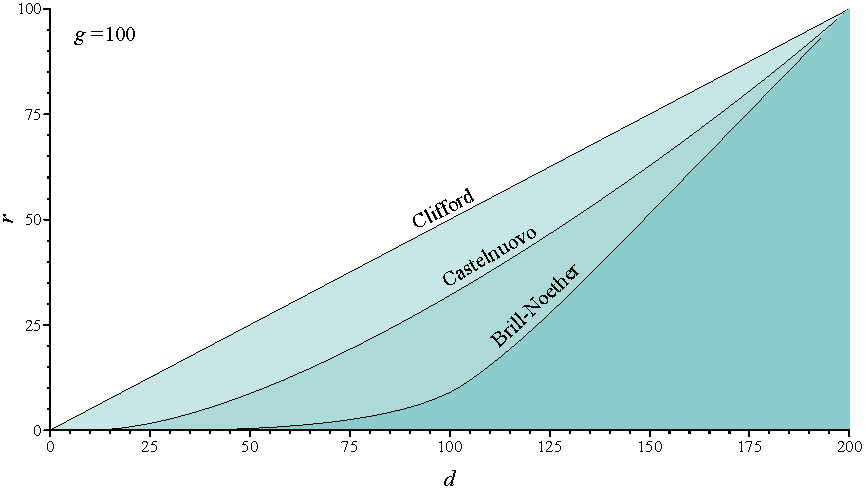
\includegraphics[width=0.9\hsize]{main/Fig11-1-new}
\caption{For smooth curves of genus 100,
these are bounds on $(d,r)$ for all linear series (Clifford),
birationally very ample series (Castelnuovo), and all linear series
on general curves (Brill--Noether).
}
\label{Clifford-Castelnuovo-BrillNoether comparison}
\end{figure}

Gathering the inequalities, and putting them all in terms of lower bounds
on $d$ given $g, r$,
we get
$$
\eqalign{
\noalign{\vskip3pt}
 d &\geq \min\{r+g, 2r\}&\quad& \hbox{ (by the Riemann--Roch and Clifford
 theorems)},\cr
\noalign{\vskip1pt}
 d &\geq \sqrt{(2r-2)\smash{g}}&& \hbox{ (by an approximation to the Castelnuovo
 theorem)},\cr
 d &\geq r+g-\frac{g}{r+1}&& \hbox{ (for a general curve)}.
}
$$

In the following sections, we'll explain the heuristic argument that
led Brill and Noether to the statement of Theorem~\ref{basic BN} and
discuss some refinements.   In Chapter~\ref{InflectionsChapter} we'll
give a proof based on the study
of inflections and on families of Jacobians.

The case $r=1$ is already interesting:

\begin{corollary}\label{gonality bound}
If $C$ is any curve of genus $g$, then $C$ admits a map  to $\PP^1$
of degree $d$ for some $d \leq \bigl\lceil \frac{g+2}{2}\bigr\rceil$.
\end{corollary}

Thus any curve of genus 2 is hyperelliptic, any curve of genus 3 or
4 is either hyperelliptic or trigonal  (admits a 3-1 map to $\PP^1$),
and so on. We have already verified this assertion in genus $g \leq 5$
by analyzing the geometry of the canonical map; for higher genera,
though, this is not feasible.

Note also that this is exactly the converse to Corollary~\ref{branched
cover BN} of Chapter~\ref{ModuliChapter}.


\subsection{A Brill--Noether inequality}\label{BN by divisors}
%12.2.1

The proof of the Brill--Noether theorem starts with a dimension
estimate that was first carried out in
\cite{Brill-NoetherOriginal}. The estimate provides an inequality on
the dimension of the variety $W^r_d$, and the assertion of the theorem
is that this is sharp for a general curve.

%From Kleiman-Laksov:  For r= 1, the matter is treated in section 4
%of Riemann's " Theorie der Abel'schen Functionen" [11] (1857) and in
%lecture 31 of Hensel-Landsberg(1902) 1; the general case is treated
%in Brill--Noether [1](1874) and in lecture 57 and appendix G of Severi
%[13].(1921)

Let $C$ be a smooth projective curve of genus $g$, and $D = p_1 + \dots
+ p_d$ a divisor on $C$. Assume for simplicity that  the points $p_i$
are distinct; the same argument  can be carried out in general, but
requires more complicated notation.

When does the divisor $D$ move in an $r$-dimensional linear series? By
the
Riemann--Roch theorem
\index{Riemann--Roch theorem}%
$h^0(D) \geq r+1$ if and only~if the vector
space $H^0(K-D)$ of 1-forms vanishing on $D$ has dimension at least
$g-d+r$\emdash that is, if and only~if the  evaluation map
$$
H^0(K) \to H^0(K|_D) = \tsty\bigoplus k_{p_i}
$$
has rank at most $d-r$.

We can represent this map by a $g \times d$ matrix. Choose a basis
$\omega_1,\dots,\omega_g$ for the space $H^0(K)$ of 1-forms on $C$;
choose an analytic open neighborhood $U_j$ of each point $p_j \in D$
and choose a local coordinate $z_j$ in $U_j$ around each point $p_j$,
and write
$$
\omega_i = f_{i,j}(z_j)\,dz_j
$$
in $U_j$. We  have $r(D) \geq r$ if and only~if the  matrix-valued
function
$$
A(z_1,\dots,z_d) =
\begin{pmatrix}
f_{1,1}(z_1) & f_{2,1}(z_1) & \dots & f_{g,1}(z_1) \\
f_{1,2}(z_2) & f_{2,2}(z_2) & \dots & f_{g,2}(z_2) \\
\vdots & \vdots &  & \vdots \\
f_{1,d}(z_d) & f_{2,d}(z_d) & \dots & f_{g,d} (z_d)
\end{pmatrix}
$$
has rank $d-r$ or less at $(z_1,\dots,z_d) = (0,\dots,0)$.


In the space $M_{d,g}$ of $d \times g$ matrices, the subset of matrices
of rank $d-r$ or less has codimension $r(g-d+r)$
\cite[Exercise 10.9]{Eisenbud1995}.
It follows
that if  an effective divisor $D$ of degree $d$ with $h^0(D) \geq r+1$
exists, then in a neighborhood of the point $D \in C_d$ the locus
$C^r_d$ of such divisors must have dimension at least $d - r(g-d+r)$,
with equality if the map $A$ is dimensionally transverse to the locus
in $M_{d,g}$ of matrices of rank at most $d-r$. Since a general fiber
\index{C@$C^r_d$}%
\index{W@$W^r_d$}%
of the map $\mu :
C^r_d
 \to
W^r_d
(C)$ has dimension $r$, it follows that
$$
\dim W^r_d(C) \geq d - r(g-d+r) - r = g - (r+1)(g-d+r)
$$
and this is exactly the  Brill--Noether (in)equality. We will give a proof
of the Brill--Noether theorem in Chapter~\ref{BrillNoetherproofChapter}.


\subsection{Refinements of the Brill--Noether theorem}

Theorem~\ref{basic BN} suggests a slew of questions, both about the
geometry of the schemes $W^r_d(C)$ parametrizing linear series on a
general curve $C$ (are they irreducible? what are their singular
loci?), and about the geometry of the linear systems themselves (do
they give embeddings? what's the Hilbert function of the image?). This
is an active area of research. Here is some of what is currently
known, starting with results about the geometry of $W^r_d(C)$:

\begin{theorem}\label{Wrd omnibus}
Let $C$ be a general curve of genus $g$,
and set
$$\rho = g - (r+1)(g-d+r).$$
Assume that $d \leq g+r$. Then:
\begin{enumerate}

\item $\dim(W^r_d(C)) = \rho$
{\rm\cite{Griffiths-Harris-BN}}.
\label{GH}

\item\label{sing wrd} The singular locus of $W^r_d(C)$ is exactly
$W^{r+1}_d(C)$
{\rm\cite{Gieseker-Petri,Lazarsfeld-Petri}}.
\label{irr wrd}

\item If $\rho > 0$ then $W^r_d(C)$ is irreducible
\index{Gieseker @Gieseker, David}%
\index{Fulton @Fulton, William}%
\index{Lazarsfeld @Lazarsfeld, Robert}%
{\rm\cite{MR611386}}.

\item\label{rho=0} If $\rho = 0$ then $W^r_d(C)$ consists of a finite
set of  points of cardinality
$$
\#W^r_d(C) = g! \prod_{\alpha=0}^r \frac{\alpha!}{(g-d+r+\alpha)!}
$$
and the monodromy of the generically finite covering of  $M_g$ by the
universal family
$\cW^r_d$ of $W^r_d$s is transitive
{\rm\cite{zbMATH04014883}}.

\item\label{Petri} If  $\sL$ is an invertible sheaf on $C$, then the
multiplication map
$$
m : H^0(L) \otimes H^0(\omega_C\otimes L^{-1}) \to H^0(\omega_C)
$$
is injective, and the Zariski tangent space to the scheme $W^r_d(C)$
at the point $L$, as a subspace
of the tangent space $T_L\pic_d(C) = H^0(\omega_C)^*` `$, is the
annihilator of the image of $m$
or, equivalently, the kernel of the dual of $m$
{\rm\cite{Gieseker-Petri}}.
\end{enumerate}
\end{theorem}

\begin{corollary}\label{2L nonspecial}
If $C$ is a general curve and $\sL$ is a general point of $W^r_d(C)$
with $r\geq 2$,
 then $\sL^m$ is nonspecial for all $m \geq 2$.
\index{nonspecial}%
\end{corollary}

\begin{proof}
If $\sL^m$ were special\emdash that is, if $\omega_C\otimes \sL^{-m}
= E$ were effective\emdash then we would have an inclusion $H^0(\sL) =
H^0(\omega_C\otimes \sL^{-m+1}(-E)) \hookrightarrow H^0(\omega_C\otimes
\sL^{-m+1})$. By part~\ref{Petri} of Theorem~\ref{Wrd omnibus}, the map
 $$
m : H^0(\sL^{m-1}) \otimes H^0(\omega_C\otimes \sL^{-m+1}) \to
H^0(\omega_C)
$$
is injective, so the map
$$
H^0(\sL^{m-1}) \otimes H^0(\sL) \subset H^0(\sL^{m-1}) \otimes
H^0(\omega_C\otimes \sL^{-m+1})
$$
obtained by restriction would likewise be injective.
However if $\sigma, \tau \in H^0(\sL)$ are two linearly independent
sections, then $\sigma^{m-1} \otimes \tau - \sigma^{m-2}\tau \otimes
\sigma$ lies in the kernel, contradicting the specialness of $\sL^m` `$.
\end{proof}
\begin{remark}
 As a special case of part~\ref{rho=0} of the theorem we see that
 the number of $g^{1}_{d}$s
 in the case $\rho=0$
(that is to say,
$g=2d-2$) is the
Catalan number
\index{Catalan number}%
 $C_{d-1}\colonequals  \tbinom{2d}{d}\big/ d$.

We have already seen this in the first two cases: in genus 2, it says
the canonical series $|K|$ is the unique $g^1_2$ on a curve of genus 2,
and in the case of genus 4 we have already seen  that there are exactly
two $g^1_3$s on a general curve of genus 4. In genus 6, it says that
a general curve of genus 6 has 5 $g^1_4$s; we'll describe these in
Section~\ref{general genus 6} below.
\end{remark}

\begin{remark}
Parts~(\ref{Petri}) and (\ref{GH}) of the theorem imply part~(\ref{sing wrd}).
\cite[Section IV.4]{ACGH} shows that at a point $\sL  \in W^r_d(C)
\setminus W^{r+1}_d(C)$, the tangent space to $W^r_d$ at the point $\sL $
is the annihilator
in $(H^0(\omega_C))^*$ of the image of $\mu$; given that $\mu$ is
injective, we can compare dimensions and deduce that $W^r_d$ is smooth
at $\sL $.
\end{remark}

\begin{remark}
For any curve $C$, there exists a scheme $G^r_d(C)$ parametrizing
linear series of degree $d$ and dimension $r$; that is, in set-theoretic
terms,
$$
G^r_d(C) = \left\{ (\sL , V) \mid \sL  \in Pic_d(C), \text{ and }
V \subset H^0(\sL ) \text{ with } \dim V = r+1 \right\}.
$$
$G^r_d(C)$ maps to $W^r_d(C)$; the map is an isomorphism over the open
subset $W^r_d(C) \setminus W^{r+1}_d(C)$ and has positive-dimensional
fibers over $W^{r+1}_d(C)$. It was conjectured
by Petri and proven in \cite{Gieseker-Petri} that for a general curve
the scheme $G^r_d(C)$ is smooth for any $d$ and $r$.
\end{remark}


Recall that  in theorems~\ref{g+1 theorem}, \ref{g+2 theorem}, \ref{g+3
theorem} we proved that
general invertible sheaves of degrees $g+1$, $g+2$ and $g+3$ on any curve
give the nicest possible maps to (respectively) $\PP^1, \PP^2$ and
$\PP^3$. These
linear series, being general of degree $\geq g$, are  nonspecial and
have respectively
2, 3, or 4-dimensional spaces of sections. The following result shows
that something
similar is true on a general curve for general linear series with 2,3,
or 4-dimensional
spaces of sections, though they may have degrees much less than $g+1,
g+2, g+3$:

\begin{npt}
\begin{theorem}[{{\cite[Proposition 5.4]{Eisenbud-Harris83}}}]
\label{grd omnibus}
Let $C$ be a general curve of genus $g$, and suppose that
$|D|$ is a general $g^r_d$ on $C$.

 \begin{enumerate}
\item If $r \geq 3$ then $D$ is very ample; that is, the map $\phi_D :
C \to \PP^r$   embeds $C$ in $\PP^r` `$;
\item If $r=2$ the map $\phi_D : C \to \PP^2$ gives a birational embedding
of $C$ as a nodal plane curve; and
\item If $r=1$, the map $\phi_D : C \to \PP^1$ expresses $C$ as a simply
branched cover of $\PP^1` `$.
\end{enumerate}
\end{theorem}
\end{npt}

In case $\rho = 0$\emdash so that there are a finite number of $g^r_d$s
on a general curve $C$\emdash these statements hold for \emph{all}
the $g^r_d$s on $C$.

In the course of investigating embeddings of a curve $C\subset \PP^n$
we have again and again
asked about the ranks of the maps $H^0(\sO_{\PP^n}(d)) \to
H^0(\sO_C(d))$. In the case of
a general curve, the following theorem of
E. Larson
\index{Larson @Larson, Eric}%
gives a
comprehensive answer,
which is the same as giving
 the Hilbert function of the image curve:

\begin{theorem}[maximal rank theorem \cite{Larson}]\label{maximal rank}
If $C$ is a general curve of genus $g$ and $\sL  \in W^r_d(C)$ is a
\index{maximal rank theorem}%
general point, then for each $m > 0$ the multiplication map
$$
\rho_m : \Sym^m H^0(\sL ) \to H^0(\sL ^m)
$$
has maximal rank; that is, it is injective if $\tbinom{m+r}{r} \leq
h^0(\sL ^m)$ and surjective if $\tbinom{m+r}{r} \geq h^0(\sL ^m)$.
\end{theorem}


If $\sL\in W^r_d(C)$ is a general point, then Corollary~\ref{2L nonspecial}
shows that $h^0(\sL ^m) = md-g+1$ for all $m \geq 2$,
and this allows us to compute the Hilbert function of a general embedding
as a curve
of degree $d$ as
 $$
 h_C(m) = \min\left(\mbinom{m+r}{r},\ md-g+1\right).
 $$

A key step in Larson's proof is an interpolation theorem \cite{MR3908670},
later extended
as follows:
\index{Larson @Larson, Eric}%
\index{Vogt @Vogt, Isabel}%

\begin{npt}
\begin{theorem}[\cite{MR4653767}]\label{Larson-Vogt}
Let $d, g$ and $r$
be nonnegative integers with $\rho(d, g, r) \geq 0$. There is a general
curve of degree $d$ and genus $g$ through $n$ general
points in $\PP^r$
if and only~if
$$
(r-1)n \leq (r + 1)@d-(r-3)(g-1)
$$
except in the four cases $(d, g, r) = (5, 2, 3)$,
$(6, 4, 3)$, $(7, 2, 5)$ and $(10, 6, 5)$.
 \end{theorem}
\end{npt}

There is a possible extension of the maximal rank theorem. If $C
\subset \PP^r$ is a general curve embedded by a general linear series,
the maximal rank theorem tells us the dimension of the $m$-th graded
piece of the ideal of $C$, for any $m$: this is just the dimension of
the kernel of $\rho_m$. But it doesn't tell us the degrees of
\index{generators of homogeneous ideal}%
generators of the homogeneous ideal of $C$. For example, if $m_0$ is
the smallest $m$ for which $I(C)_m \neq 0$, or numerically the
smallest $m$ such that $\tbinom{m+r}{r} > md-g+1$, we can ask: is the
homogeneous ideal $I(C)$ generated by $I(C)_{m_0}$? This can't always
be the case, since
there are examples where the  smallest nonzero graded piece of $I(C)$ has
dimension 1. But one might conjecture that $I(C)$ is always be generated
by its graded pieces of degrees $m$ and $m+1$; this is an open problem.

To answer this, given that we know the dimensions of $I(C)_m$ for
every~$m$, we would need to know the ranks of the multiplication
maps
$$
\sigma_m : I(C)_m \otimes H^0(\cO_{\PP^r}(1)) \to I(C)_{m+1}
$$
for each $m$. In particular, we may conjecture that \emph{the maps
$\sigma$ have maximal rank}; if this were true we could deduce the
\index{maximal rank}%
degrees of a minimal set of generators for the homogeneous ideal $I(C)$.

Another recent strand of work on Brill--Noether theory was developed in
the thesis
\cite{HLarson} and in \cite{arXiv:2008.10765}, providing  analogues of
many of the parts of the classical Brill--Noether theorem
\index{Brill--Noether theory|)}%
\index{Brill--Noether theorem!for curves of given gonality}%
\index{gonality}%
for general curves of given gonality in the cases $\rho\geq 0$.

There are many remaining questions! One is the question of \emph{secant
planes}: a naive dimension count would suggest that an irreducible,
nondegenerate curve $C \subset \PP^r$ should have an $s$-secant $t$-plane
if and only~if $s(r-t-1) \leq (t+1)(r-t)$
(for example a curve $C \subset \PP^3$ has 4-secant lines, but no
5-secant lines; see Exercise~\ref{out of place}). 
Is this true for a general curve embedded in $\PP^r$
by a general linear series?

\section{Linear series on curves of genus 6}
\label{genus 6 section}\label{general genus 6}

We have seen in our analysis of curves of genus up to 5 that curves of the
same genus can look quite different from the point of view of the linear
series they possess: the existence of $g^r_d$s,  the geometry of the
schemes $W^r_d(C)$ parametrizing them, and the geometry of the associated
maps to projective space, can look quite different on different curves.

The variety of possible behaviors has increased modestly with the
genus. Genus 6 is a tipping point: we could still enumerate all the
possible behaviors of the schemes $W^r_d(C)$\emdash as distinguished
by the number of components, dimension and singularities of the various
schemes $W^r_d(C)$, and the geometry of the associated maps\emdash but
it's quite a long list, and we will actually study just a few cases. For
genus 7 and higher a full analysis has probably never been carried out.

In lower genus we tacitly verified the statements of the Brill--Noether
theorem from our descriptions of the canonical models. In genus 6, by
contrast, we cannot  deduce the Brill--Noether theorem from studying
the geometry of the canonical curve\emdash though we can easily see that
a canonical curve $C \subset \PP^5$ of genus 6 lies on a 6-dimensional
vector space of quadrics, that doesn't tell us much about its geometry.

Instead we will appeal directly to the Brill--Noether theorems. Here is
a summary of what we will use:

\begin{theorem}\label{BN consequences}
Every smooth curve $C$ of genus 6 has at least one $g^{2}_{6}$. If $C$
is general, then
$W^{2}_{6}(C)$ and $W^{1}_{4}(C)$ each consist of 5 reduced points,
while $W^{2}_{5} = W^{1}_{3} = \emptyset$.  Less formally, C has
precisely 5 $g^{2}_{6}$s and 5 $g^{1}_{4}$s, but no $g^{2}_{5}$s and
no $g^{1}_{3}$s. The image of the map associated to each $g^{2}_{6}$
is a nodal plane curve and its nodes are in linearly general position,
that is, no three are collinear.
\end{theorem}

All these assertions except for the linear general position of the nodes
follow immediately from
Theorem~\ref{basic BN} and
Theorem~\ref{Wrd omnibus}; we will deduce the linear general position
of the nodes from the relationship of the different
linear series on a general curve that are given by these theorems.

%\subsection{Linear series on general curves of genus 6}\label{general genus 6}
\subsection{General curves of genus 6}
\emph{We suppose for the rest of this section that $C$ is a general
smooth curve of genus 6.}

By Theorem~\ref{BN consequences} we can map $C$ birationally to a plane
sextic $C_0$ with only nodes as singularities. Since a plane sextic has
arithmetic genus $\tbinom{6-1}{2} = 10$, the curve $C_{0}$
must have exactly 4 nodes.

Once we have exhibited one birational map of $C$ to a plane sextic with
4 nodes, we can describe all five $g^2_6$s and all five $g^1_4$s in terms
of this plane model. For example, composing a $g^1_6$ corresponding to $f:
C\to \PP^1$ with the projections from the 4 nodes gives four $g^1_4$s. To
see the
fifth
$g^{1}_{4}$ we introduce some terminology:

Suppose $f : X \to S$ is a regular map from any smooth curve $X$ to a
surface $S$. If $\sL $ is a line bundle on $S$ and $V \subset H^0(\sL
)$ a vector space of sections, we can associate to them a linear system
on $X$ by taking the pullback linear system $f^*V \subset H^0(f^*\sL )$
on $X$ and subtracting the basepoints; this is called the
\emph{linear series cut out on $X$ by $V$}.
\index{linear series!cut out on $X$ by $V$}%

\begin{figure}[b]
\hskip0pt
\raise3pt\hbox{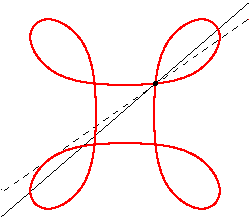
\includegraphics[width=0.36\hsize]{main/Fig11-2-new}\quad}
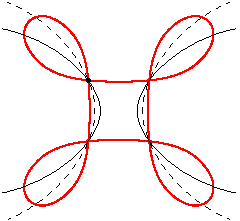
\includegraphics[width=0.34\hsize]{main/Fig11-3-new}
\caption{Left: A $g^1_4$ as (left)
the projection from a node of a plane sextic
and (right)
a pencil of conics through the four nodes of a
plane sextic.
}
\label{plane sextic 1}
\end{figure}

To see the $g^{1}_{4}$s on $C$ in this way,  suppose again that $C$ is a
general curve of genus 6 as above and $f : C \to \PP^2$ is a birational
map onto a sextic curve $C_0$ with four nodes; let $p \in C_0$ be one of
the nodes and consider the linear system $(\cO_{\PP^2}(1),V)$ of lines
in $\PP^2$ through $p$. The pullback $f^*\cO_{\PP^2}(1)$ of course has
degree 6, but the pullback linear series $f^*V$ has two basepoints,
at the points $q, r \in C$ lying over $p$. The linear series cut on $C$
by $V$ is thus a $g^1_4$; see Figure~\ref{plane sextic 1}, left.

To produce the fifth $g^1_4$, consider the linear series cut on
$C$ by conic plane curves passing through all four nodes of $C_0$
(Figure~\ref{plane sextic 1}, right).  There is a pencil of such conics, and
the pullback $f^*\cO_{\PP^2}(2)$ has degree 12.
If the nodes are linearly independent then the pullback series has eight
basepoints; thus we arrive at another $g^1_4$ on $C$.  Not all the nodes
can be contained in a line, since then, by B\'ezout's theorem, the line
\index{Bezout@B\'ezout's theorem}%
would be a component of $C_0$. Thus if the nodes are linearly dependent,
then exactly 3 lie on a line
so the linear series cut by the conics containing the nodes coincides
with the projection from the
fourth
node.
This would represent a nonreduced point of the scheme $W^1_4(C)$,
the subject of Exercise~\ref{nonreduced Wrd} below. Thus the nodes
are independent.

For another example, consider the linear system cut on $C$ by cubics
passing through all four nodes. This has degree $3\cdot 6 - 8 = 10$
and dimension 6. It follows that this is the
complete canonical series
\index{complete canonical series}%
on $C$. (In Chapter~\ref{PlaneCurvesChapter} we will see directly that
this is the case.)

Given the degree six map $f : C \to C_0 \subset \PP^2$ corresponding
to one $g^2_6$ we can use the fact that the five $g^2_6$s on $C$ are
residual to the five $g^1_4$s in the canonical series to construct the
other four $g^2_6$s: they are cut out on $C$ by the linear system of plane
conics passing through three of the four nodes of $C_0$  Equivalently,
their images are the curves obtained from $C_{0}$ by the quadratic
transformation
of $\PP^{2}$ centered at 3 of the 4 nodes, which blows up these 3 nodes
and blows down the three lines
 joining them (Figure~\ref{plane sextics 3}).

 In previous chapters we have seen that in genus $\leq 5$ a general
 canonical curve is  a complete intersection, but this fails for a
\index{complete intersection}%
 canonical curve $C$ of genus 6. There is a 21-dimensional vector space of
quadratic forms on $\PP^5` `$, and $h^0(\sO_C(2)) = 2(2g-2)-g+1 = 15$,
so $C$ lies on at least 6 quadrics, and we will show that its ideal sheaf
is generated by exactly 6 quadrics. Since $6>\codim C$, the canonical
curve of genus 6 is not a complete intersection. However, such curves
lie on a quintic del Pezzo surface, which may be described as follows.
\index{del Pezzo surface}%
\index{del Pezzo surface!quintic|(}%

%There is a further consequence of this description: the four nodes of
%$C_0$ are in linear general position; that is, no three are collinear.
%By parts~(\ref{rho=0}) and~\ref{Petri} of Theorem~\ref{Wrd omnibus}, $C$
%must have 5 distinct $g^1_4$s, and if three of the four nodes of $C_0$
%were collinear, the $g^1_4$ cut on $C$ by lines through the fourth node
%would coincide with the $g^1_4$ cut on $C$ by conics through all four.

\begin{figure}
\centerline {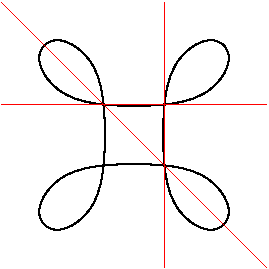
\includegraphics[height=1.5in,trim=10 10 10 10,clip]{main/Fig11-4-new}}
\caption{A sextic with 4 nodes and the fundamental triangle of the
quadratic transformation giving
a different $g^{2}_{6}$.}
\label{plane sextics 3}
\end{figure}


\subsection{Del Pezzo surfaces}\label{Del Pezzo sketch}
%12.3.2

We  met the del Pezzo surface of degree 5 in Section~\ref{Genus 1 quintics
in P4}.
We briefly sketch, without proofs, a little of the
 rich classical theory of del Pezzo surfaces in general. The basics are
 well treated in \cite[pp.~45--50]{Beauville}; for more, see the
beautiful book \cite{Manin}, which also goes into some of the arithmetic
\index{Manin, Yuri I.}%
\index{Beauville @Beauville, Arnaud}%
theory. We will use only the case of the del Pezzo surface of degree 4,
which lies in $\PP^{5}$

By definition,
a \emph{del Pezzo} surface is a smooth surface embedded in $\PP^n$  by
its complete anticanonical series $-K_S$. These exist only for $3\leq
n\leq 9$. The best-known example is a smooth cubic surface in $\PP^3``$.
That it is a del Pezzo surface follows from the adjunction formula.

A del Pezzo surface in $\PP^n$ has degree $n$, and is isomorphic to the
blow-up of $\PP^2$ at $9-n$ points of which no 3 lie on a line and no
6 lie on a conic, embedded by the linear series on $\PP^2$
consisting of the cubics passing through the $9-n$ points\emdash except
when $n=8$, in which case the
linear series of curves of type $(2,2)$ on $\PP^1\times \PP^1$ provides
another example.

Comparing the linear series  of cubic forms containing $p_1,\dots,p_4$
with the linear series  of sextic forms vanishing to order 2 at
$p_1,\dots,p_4$, we see that a quintic del Pezzo surface $S \subset \PP^5$
lies on at least $5$ quadrics. In fact, its homogeneous ideal is generated
by exactly 5 quadrics.

A quintic del Pezzo surface $S \subset \PP^5$ contains exactly 10 lines,
which (in terms of the description of $S$ as the blow up of $\PP^2$ at
four points $p_1,\dots,p_4 \in \PP^2$) are the 4 exceptional divisors
and the 6 proper transforms of the lines joining the $p_i$ pairwise. The
configuration of these lines is shown in Figure~\ref{dual graph of the
configuration of 10 lines on a quintic del Pezzo surface}.
It is the intersection of a $\PP^5$ with the Grassmannian $G(2,5)
\subset \PP^9` `$, and correspondingly the five quadrics containing $S$
can be realized as the Pfaffians of a  $5\times 5$ skew-symmetric matrix
of linear forms on $\PP^5` `$.

\begin{figure}
\centerline {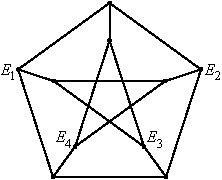
\includegraphics[height=1.4in]{main/Fig11-5}}
\caption{Dual graph of the configuration of 10 lines on a quintic del
Pezzo surface, the plane blown up
at 4 points showing 4 pairwise disjoint exceptional divisors.}
\label{dual graph of the configuration of 10 lines on a quintic del
Pezzo surface}
\end{figure}

There is also a notion of a \emph{weak del Pezzo}
\index{weak del Pezzo}%
surface; this is a
smooth surface whose
anticanonical bundle
\index{anticanonical bundle}%
 is
nef but not necessarily ample.
\index{nef but not necessarily ample}%
We get such a surface if we blow up $\PP^2$ at a configuration
of points of which three are collinear; in this circumstance the
anticanonical bundle on the blow-up $S$ has degree 0 on the proper
transform of the line containing the three points, and this proper
transform is correspondingly collapsed to a rational double point of the
image $\phi_{-K}(S)$. In general, the description of del Pezzo surfaces
as blow-ups of the plane extends to the case of weak del Pezzos.



\subsection{The canonical image of a general curve of genus 6}

Using the Brill--Noether theorem, we have seen that a general curve $C$
of genus 6 is the normalization of a plane sextic $C_0$ with four nodes,
and that the canonical series on $C$ is cut out by cubics in the plane
passing through the four nodes. Thus the canonical model lies on the
surface $S \subset \PP^5$ that is the image of the plane under the
(rational) map given by cubics through these four points, which we now
recognize as a quintic del Pezzo surface.

\begin{theorem}
A general canonical curve $C$ of genus 6 is the intersection of a quintic
del Pezzo surface and a quadric.
\end{theorem}

\begin{proof}
We have seen that $C \subset \PP^5$ lies on a quintic del Pezzo surface
\index{del Pezzo surface!quintic|)}%
$S \subset \PP^5` `$. The surface is cut out by 5 quadrics, and we know
that $C$ lies on 6 independent quadrics,
so $C$ is contained in the complete intersection of $S$ with a
quadric. Since this scheme has degree 10, which is the degree of $C$,
they are equal.
\end{proof}

For corresponding theorems for general curves with $g=7,8,9$ see
\cite{Mukai1}, \cite{Mukai2}, and \cite{Mukai3}.


\section{Classification of curves of genus 6}

From Theorem~\ref{BN consequences} we know that every curve $C$ of genus
6 has  a $g^{2}_{6}$. For a general curve the corresponding morphism
$\phi_{D}$ maps $C$ birationally onto a plane sextic with 4 nodes and
exactly 5 $g^{1}_{4}$s.
In this  section we will analyze some of the other curves of genus 6,
starting with the question  ``what could go wrong?''
with the birational map to $\PP^2` `$.

Since we already have a complete picture in the hyperelliptic case, we'll
assume that $C$ is nonhyperelliptic. Clifford's theorem then rules out
the existence of a $g^3_6$ so  the $g^2_6$ is a complete linear series
$|D|$ for some divisor $D$ of degree 6.

Further analysis can be divided as follows:
\smallbreak
\noindent\underline{Case 1}:
$C$ is not
trigonal.
\index{trigonal}%
\begin{enumerate}\def\theenumi{\alph{enumi}}
 \item $|D|$ has a basepoint; the canonical image of $C$ lies on the
 Veronese surface.
\item $\phi_{D}$ maps $C$
two-to-one
\index{2-sheeted cover}%
onto a cubic $E \subset \PP^2$ of
genus 1; the canonical image is the
complete intersection
\index{complete intersection}%
of a quadric
and the
cone over the elliptic quintic
\index{cone!over elliptic quintic}%
\index{quintic!elliptic}%
$E\subset \PP^{4}$.
\item $\phi_{D}$ is birational onto a plane sextic with no triple point.
 \end{enumerate}
\noindent\underline{Case 2}:
$C$ is trigonal. The canonical image lies on a
rational normal scroll $S(a,4-a)$; see Chapter~\ref{ScrollsChapter}.
In this case $|D|$ is basepoint free and $\phi_{D}$  either maps $C$
three to one onto a conic
 or birationally onto a
sextic with a triple point.
\index{3-sheeted cover!of conic}%
\index{sextic!with triple point}%
\index{triple point!on sextic}%
\smallbreak

In the rest of this section we will examine cases 1(a) and 1(b). Case 2 can
be further divided by the value of $a$.
Case 1(c) may be divided into many parts according to the various
configurations
of double points of the plane sextic, which may be nodes, cusps, tacnodes
or higher-order double points,  corresponding to various possible
schemes $W^{1}_{4}$.

The analysis of the other cases is lengthy, but largely accessible with
the tools we've introduced.


\subsection*{$|D|$ has a basepoint}
%\label{g26 has a basepoint}

Clifford's theorem shows that a nonhyperelliptic curve of genus 6 cannot
have a $g^2_4$, so
$|D|$ has exactly one basepoint, and when we subtract the basepoint we
get a basepoint-free $g^2_5$.

If $C \to C_0 \subset \PP^r$ is the map given by a basepoint free $g^r_d$,
the degree $d$ of the linear series is the degree of the image curve $C_0$
times the degree of the map $C \to C_0$. Since 5 is prime, the associated
map $\phi_D : C \to \PP^2$ is birational onto a quintic curve. Moreover,
since
\index{plane quintic}%
plane quintic
 curves have
arithmetic genus 6,
\index{arithmetic genus}%
the image $\phi_D(C)$
is smooth; thus $C$ is isomorphic to a smooth plane quintic.

This allows us to describe the other special linear series on $C$. By
the adjunction formula, the canonical series $|K_C|$ is cut on $C$
by conics in the plane.

The plane $\PP^2$ is embedded by the complete linear series of quadrics
as the
{Veronese surface in $\PP^5``$,
\index{Veronese!surface!in $\PP^5$}%
of $C$ is cut out by quadrics, the canonical model of $C$
lies on this surface, and the canonical ideal is generated by the
6-dimensional family of quadrics containing the Veronese surface\emdash
the $2\times 2$ minors of the generic symmetric $3\times 3$ matrix
corresponding to the multiplication map
$$
H^{0}(\sO_{\PP^{2}}(1)) \otimes H^{0}(\sO_{\PP^{2}}(1)) \to
H^{0}(\sO_{\PP^{2}}(2))
$$
as explained in Proposition~\ref{some equations}-- together with a
3-dimensional family of cubics,  the image of the 3 dimensional family
of forms of degree 6 that are multiples of the quintic form defining $C$
in $\PP^2` `$.

As we showed in Chapter~\ref{3b}, the $g^1_4$s on $C$ are exactly the
projections from points of $C$, so $W^1_4(C)\cong C$, and there are no
$g^{1}_{3}$s.


\subsection*{$C$ is not trigonal and the image of
\texorpdfstring{$\phi_{D}$}{phi(D)} is two-to-one onto a  plane curve
of degree 3.}

The cubic curve $E$ is smooth since otherwise it would have geometric
genus 0 and $C$ would be  hyperelliptic. Thus $C$ is a double cover of
a smooth curve of genus 1; we say that $C$ is \emph{bielliptic}.
\index{bielliptic}%

In this case the canonical divisor class $K_C$ is the pullback of
an invertible sheaf $\cO_E(F)$ for some divisor class of degree 5 on
$E$. But it is not the case that the canonical series $|K_C|$ is the
pullback of the linear series $|\cO_E(F)|$: by the Riemann--Roch theorem,
the latter has dimension 4, rather than 5. Indeed, if we recall that
the target of the canonical map $\phi_K : C \to \PP^5$ is the projective
space $\PP H^0(K_C)$, there is be a point $X \in \PP^5$ corresponding to
the hyperplane $\pi^*H^0(F) \hookrightarrow H^0(K_C)$, and projection
of the canonical curve from this point maps $C$ 2-to-1 onto the image
$\phi_F(E) \subset \PP^4` `$. In other words, the canonical model of $C$
lies on a cone $S = \overline{X, E}$ over an elliptic normal quintic
curve $E \subset \PP^4` `$.

As we saw in Chapter~\ref{3b}, the quintic curve $\phi_F(E) \subset \PP^4$
lies on 5 quadrics, as does the cone $S \subset \PP^5$ over it. Thus
there is a quadric $Q \subset \PP^5$ containing $C$ but not containing
$S$. B\'ezout's theorem shows that in this case, the canonical model of
a bielliptic curve of genus 6 is the intersection of the cone over an
elliptic quintic curve with a quadric.

\section{Exercises}

\begin{exercise}
\label{out of place}
We saw in Chapter~\ref{JacobianChapter} that if $C$ is any curve of genus
$g$ and $D$ a general divisor of degree $g+3$ on $C$, then $\phi_D :
C \hookrightarrow \PP^3$ is an embedding. Using the Brill--Noether
theorem, show that if $C$ is general then the image curve in $\PP^3$
has no 5-secant lines.
\end{exercise}

\begin{exercise}
Let $C$ be a bielliptic curve of genus 6; that is, a double cover of a
\index{bielliptic}%
smooth projective curve $E$ of genus 1.
\begin{enumerate}
\item Show that $C$ cannot be hyperelliptic (going forward, we will
identify $C$ with its canonical image in $\PP^5$).
\item Let $F$ an invertible sheaf of degree 5 on $E$ and $\phi_F(E)
\subset \PP^4$ the corresponding elliptic normal quintic curve. Show that
$\phi_F(E)$ lies on 5 quadrics, as does the cone $S \subset \PP^5$ over it.
\tohint{12-02}
\item Deduce that there is a quadric $Q \subset \PP^5$ containing $C$
but not containing $S$. Now invoke B\'ezout's theorem to deduce that in
this case, the canonical model of a bielliptic curve of genus 6 is the
intersection of the cone over an elliptic quintic curve with a quadric.
\end{enumerate}
\end{exercise}

\begin{exercise}
Use the preceding exercise to show that if $C$ is a bielliptic curve of
genus 6, a 2-sheeted cover of an elliptic curve $E$, then every $g^1_4$
on $C$ is the pullback of a $g^1_2$ on $E$, and likewise  every $g^2_6$
on $C$ is the pullback of a $g^2_3$ on $E$. Deduce that in this case,
$W^1_4(C)$ and $W^2_6(C)$ are each isomorphic to $E$.
\tohint{12-03}
\end{exercise}

\begin{exercise}
Let $C$ be a trigonal curve of genus 6 with $g^1_3$ $|E|$, and $p \in C$
a general point. Show that the linear series $|K_C - E-p|$ is a $g^2_6$,
and that the corresponding map $C \to \PP^2$ maps $C$ birationally onto
a plane sextic curve with a triple point.
\end{exercise}

\begin{exercise}\label{plane models}
Let $C$ be the normalization of a plane sextic $C_0$ with four nodes,
three of which are collinear. Show that by choosing a different $g^2_6$
on $C$, we can express it as the normalization of a plane sextic with
two nodes and a tacnode.
\tohint{12-05}
\end{exercise}

\begin{exercise}
Show that if $C$ is the normalization of a plane sextic $C_0$ with only
double points, then $W^1_4(C) \cong W^2_6(C)$ is zero-dimensional (so
in particular this case does not overlap with any of the previous cases)
\end{exercise}

\begin{exercise}
Find an example of a curve $C$ of genus 6 such that $W^1_4(C)$ consists
of one point of degree 5. Bonus points for showing that in this case
the scheme $W^1_4(C) \cong \Spec \CC[\epsilon]/(\epsilon^5)$.
\tohint{12-07}
\end{exercise}

\begin{exercise}
Show that if $C$ is a smooth plane quintic, then the $g^2_6$s on $C$
all have a basepoint; that is, they are all of the form $|K_C| + p$
for $p \in C$.

Furthermore, the canonical model of $C$ will lie on a quadratic Veronese
surface $S$; and the six
quadrics containing the canonical curve $C$ are the six quadrics
containing $S$.
In particular, the intersection of the quadrics containing
$C$ will be $S$, so
the ideal of $C$ requires generators of degree $>2$.
\end{exercise}

\begin{exercise}\label{nonreduced Wrd}
Show that if the nodes of the curve $C_0$ are in linear general
position\emdash that is, no three
are
collinear\emdash then indeed the map
$$\mu : H^0(D) \otimes H^0(K-D) \to H^0(K)$$ is an isomorphism for each
of the five $g^1_4$s on $C$.
\end{exercise}


%header and footer for separate chapter files

\ifx\whole\undefined
\documentclass[12pt, leqno]{book}
\usepackage{graphicx}
\input style-for-curves.sty
\usepackage{hyperref}
\usepackage{showkeys} %This shows the labels.
%\usepackage{SLAG,msribib,local}
%\usepackage{amsmath,amscd,amsthm,amssymb,amsxtra,latexsym,epsfig,epic,graphics}
%\usepackage[matrix,arrow,curve]{xy}
%\usepackage{graphicx}
%\usepackage{diagrams}
%
%%\usepackage{amsrefs}
%%%%%%%%%%%%%%%%%%%%%%%%%%%%%%%%%%%%%%%%%%
%%\textwidth16cm
%%\textheight20cm
%%\topmargin-2cm
%\oddsidemargin.8cm
%\evensidemargin1cm
%
%%%%%%Definitions
%\input preamble.tex
%\input style-for-curves.sty
%\def\TU{{\bf U}}
%\def\AA{{\mathbb A}}
%\def\BB{{\mathbb B}}
%\def\CC{{\mathbb C}}
%\def\QQ{{\mathbb Q}}
%\def\RR{{\mathbb R}}
%\def\facet{{\bf facet}}
%\def\image{{\rm image}}
%\def\cE{{\cal E}}
%\def\cF{{\cal F}}
%\def\cG{{\cal G}}
%\def\cH{{\cal H}}
%\def\cHom{{{\cal H}om}}
%\def\h{{\rm h}}
% \def\bs{{Boij-S\"oderberg{} }}
%
%\makeatletter
%\def\Ddots{\mathinner{\mkern1mu\raise\p@
%\vbox{\kern7\p@\hbox{.}}\mkern2mu
%\raise4\p@\hbox{.}\mkern2mu\raise7\p@\hbox{.}\mkern1mu}}
%\makeatother

%%
%\pagestyle{myheadings}

%\input style-for-curves.tex
%\documentclass{cambridge7A}
%\usepackage{hatcher_revised} 
%\usepackage{3264}
   
\errorcontextlines=1000
%\usepackage{makeidx}
\let\see\relax
\usepackage{makeidx}
\makeindex
% \index{word} in the doc; \index{variety!algebraic} gives variety, algebraic
% PUT a % after each \index{***}

\overfullrule=5pt
\catcode`\@\active
\def@{\mskip1.5mu} %produce a small space in math with an @

\title{Personalities of Curves}
\author{\copyright David Eisenbud and Joe Harris}
%%\includeonly{%
%0-intro,01-ChowRingDogma,02-FirstExamples,03-Grassmannians,04-GeneralGrassmannians
%,05-VectorBundlesAndChernClasses,06-LinesOnHypersurfaces,07-SingularElementsOfLinearSeries,
%08-ParameterSpaces,
%bib
%}

\date{\today}
%%\date{}
%\title{Curves}
%%{\normalsize ***Preliminary Version***}} 
%\author{David Eisenbud and Joe Harris }
%
%\begin{document}

\begin{document}
\maketitle

\pagenumbering{roman}
\setcounter{page}{5}
%\begin{5}
%\end{5}
\pagenumbering{arabic}
\tableofcontents
\fi


\chapter{Inflection points}\label{inflections chapter}
\label{InflectionsChapter}

Generalizing the ramification points of a map from a smooth curve $C$
\index{flex|see inflection point}%
to $\PP^1` `$, there are finitely many ``special'' points determined by
any linear series on any curve, the \emph{inflection points}.
\index{inflection point}%
We love this topic for its echoes of classical algebraic geometry and
it will provide the tools to give a proof of the Brill--Noether
theorem in the following chapter. In characteristic 0 every linear
series has finitely many inflection points, and the number of these,
properly counted, depends only on the genus of the curve and the
degree of the linear series.

\section{Inflection points,  Pl\"ucker formulas and Weierstrass points}

\subsection*{Definitions}
To characterize the inflection points of a linear series
$\sD = (\sL, V)$ on a curve $C$, we will use the following result:

\begin{proposition}\label{vanishing sequence} Let $V$ be a
\index{vanishing sequence}%
  finite-dimensional vector space of
global sections
\index{global section}%
of an
invertible sheaf
\index{invertible sheaf}%
$\sL$ on a smooth curve $C$, and let $p \in C$
be a point. There exists a basis $\sigma_0, \dots, \sigma_r$ of $V$
consisting of sections vanishing to different orders at~$p$. Thus the set
$$
\{ \ord_p(\sigma) \mid \sigma \neq 0 \in V \}
$$
 has cardinality $\dim V` `$.
\unif
\end{proposition}

\begin{proof}
Let $\tau_0, \dots, \tau_r$ be any basis of $V` `$.  If  $\tau_i$ and
$\tau_j$ vanish to the same order at~$p$, then
some nonzero linear combination $\tau_i' \colonequals  a\tau_i+b\tau_j$
vanishes to strictly higher order. Since the coefficients $a$ and $b$
are both necessarily nonzero we may modify the basis, replacing $\tau_i$
with $\tau_i'$, strictly increasing the sum of the orders.
The order of vanishing of each $\sigma_i$ is bounded above by $\deg \sL$,
so the sum of the orders is bounded by $(r+1)\deg \sL$. Thus the process
must terminate, and when it does,
 the orders must be distinct.
\end{proof}

According to  Proposition~\ref{vanishing sequence}, if $\cD = (\cL, V)$
is any $g^r_d$ on $C$, we may write
$$
\{ \ord_p(\sigma) \mid \sigma \neq 0 \in V \} = \{a_0,\dots,a_r\} \;
\text{ with } \; 0\leq a_0 < a_1 < \dots < a_r.
$$
The sequence $a_i = a_i(\cD,p)$ is called the
\index{vanishing sequence|defi}%
\emph{vanishing sequence} of $\cD$ at $p$.  Since $a_i \geq i$,
the numbers
$\alpha_i = \alpha_i(\cD,p) \colonequals  a_i - i$ are often more
interesting,
and the sequence $0 \leq \alpha_0 \leq \alpha_1 \leq \dots \leq
\index{ramification sequence|defi}%
\alpha_r$ is called the \emph{ramification sequence} of $\cD$ at $p$.

We say that $p$ is an \emph{inflection point} of the linear series $\cD$
if $(\alpha_0,\dots,\alpha_r) \neq (0,\dots,0)$\emdash equivalently,
if $\alpha_r > 0$\emdash and we define the \emph{weight} of $p$ to be
\index{weight!of an inflection point}%
$$
w(\cD, p) = \sum_{i=0}^r \alpha_i(\cD, p)
$$
and the
\emph{inflectionary divisor}
\index{inflectionary!see divisor, inflectionary}%
\index{divisor!inflectionary}%
 on $C$ to be
$$
\sum_{p\in C}w(\cD, p)p.
$$

If $\cD$ is very ample, so that it may be viewed as the linear series cut
on $C$ by hyperplanes for some embedding $C \subset \PP^r` `$, then $p$
is an inflection point if $a_r > r$; that is, if there is a hyperplane
$H \subset \PP^r$ having contact of order $r+1$ or more with $C$ at $p$.

The first two terms in the ramification sequence are particularly
important: $\alpha_0(\cD, p)$ is nonzero if and only~if $p$ is a basepoint
of $\cD$; and if $\alpha_0(\cD, p)=0$, then $\alpha_1(\cD, p) = 0$ if
and only~if, in addition, the map $\phi_\cD$ is an
immersion
\index{immersion}%
(that is,
has nonzero derivative) at $p$.

\subsection*{The Pl\"ucker formula}

In characteristic 0, a linear series on a smooth projective curve can
\index{inflection point!--s are finite in number in characteristic zero}%
have only finitely many inflection points (this can be proven
directly just as in Lemma~\ref{finite inflections}), and indeed the
sum of the weights of all the inflection points depends only on the
genus of the curve and the degree and dimension
of the linear
series. This is the Pl\"ucker formula:

\begin{theorem}\label{Plucker}
If $C$ be a smooth curve of genus $g$ and $\cD$ is a
\index{Pl\"ucker formula}%
linear series of degree $d$ and dimension $r$, then
$$
\sum_{p \in C} w(\cD, p) \; = \; (r+1)d + r(r+1)(g-1).
$$
\end{theorem}

For a proof, see for example \cite[Theorem 7.13]{3264}.

Theorem~\ref{Plucker} also holds in positive characteristic under the
positive characteristic
\index{positive characteristic}%
hypothesis that the number of inflection points is finite (equivalently,
not every point is an inflection point). This may seem like an unnecessary
hypothesis\emdash it's hard to imagine a plane curve in which every
point is a flex!\emdash but in positive characteristic there are such curves;
see Exercise~\ref{inseparable Gauss}.

As an immediate consequence of the Pl\"ucker formula, we have:

\begin{corollary}\label{uninflected curves}
 If $C\subset \PP^r$ is a smooth nondegenerate curve with no inflection
 points, then $C$ is the
rational normal curve
\index{rational normal curve}%
of degree $r$.
\unif
\end{corollary}

\begin{proof}
Suppose $C \subset \PP^r$ is a curve of degree $d$ and genus $g$. If $C$
has no inflection points then, by the Pl\"ucker formula, we must have
$$
(r+1)d + r(r+1)(g-1) = 0.
$$
This immediately implies that $g=0$, so that we must have $(r+1)(d-r)
= 0$ and hence $d=r$; thus $C$ is a rational normal curve.
\unif
\end{proof}

\begin{corollary}
A nondegenerate smooth  curve $C\subset \PP^{r}$ is the rational normal
curve
of degree $r$ if and only~if any of the following equivalent properties
holds:
\begin{enumerate}
\item $C$ is
\index{projectively homogeneous}%
projectively homogeneous.
\item $C$ has no inflection points.
\item Every subscheme of length $r+1$ contained in $C$ spans $\PP^{r}$.
\unif
\end{enumerate}
\end{corollary}

\begin{proof}
Corollary~\ref{uninflected curves} implies that the
rational normal curves are the only ones without any inflection points.

By Proposition~\ref{Veronese is projectively homogeneous}, the rational
normal curve
is projectively homogeneous. On the other hand, since not every point
on $C$ is an inflection point, a curve with an inflection point cannot
be projectively homogeneous.

If $p \in C$ is an inflection point, then $(r+1)p$ is  a subscheme that
lies in a hyperplane
whereas in Proposition~\ref{independence of points on a RNC} we showed
that if $C \subset \PP^r$ is a rational normal curve, and $\Gamma
\subset C$ any proper subscheme of $C$ of degree $r+1$, then $\Gamma$
spans $\PP^r` `$.
\end{proof}

The Pl\"ucker formula leaves many questions about the possible
configurations of flex points unanswered.
For example, how many cusps can there be on a plane curve of geometric
genus $g$ and degree $d$? See
Figure~\ref{3 real cusps} for the maximum possible on a curve of degree 4.
The answer is known only up to degree 8:
Zariski
\index{Zariski!Oskar}%
\index{Calabri, Alberto}%
\index{Kulikov, Viktor S.}%
\index{Shustin, Eugenii}%
\index{Kharlamov, Viatcheslav}%
\index{Sottile, Frank}%
\citeyear{Zariski1931}
proved
that
a plane curve of degree 8 can have 15 but not 16 cusps.
See \cite{Calabri} and \cite{Kulikov} for recent contributions and
\cite{Kharlamov-Sottile} for a study of what is possible
over the real numbers.

\begin{figure}\label{3-cusp quartic}
\includegraphics[scale=.7]{"main/deltoid"}
\caption{The deltoid is a quartic plane curve with three cusps and
  $S_3$ symmetry. Its
affine equation is $(x^2+y^2)(x^2+y^2+18)+8y(y^2-3x^2)-27=0$.
}
 \label{3 real cusps}
\end{figure}

One thing we do know is the behavior of the inflection points for a
general linear series on a general curve; we will state this here and
prove it as a corollary to the proof of the Brill--Noether theorem in
Chapter~\ref{BrillNoetherproofChapter}:

\begin{theorem}\label{Brill Noether Plucker}
If $C$ is a general curve of genus $g$, $\sL \in W^r_d(C) \subset
\pic_d(C)$ a general line bundle of degree $d$ with $h^0(\sL) = r+1$ and
$V = H^0(\sL)$, then every inflection point of the linear series $\cD =
(\sL, V)$ has weight 1 and hence ramification sequence $(0, \dots, 0, 1)$.
\end{theorem}


\subsection*{Flexes of plane curves}
\label{plane curve pluecker}

Specializing Theorem~\ref{Plucker} to a smooth curve of degree $d$
in the plane, and using the formula
$g= \tbinom{d-1}{2}$, we see that the total number of flexes is $3(d-2)d$.

It turns out that the
inflectionary divisor
\index{divisor!inflectionary}%
$\sum w(C, p)p$
is the intersection of $C$ with a curve of degree $3(d-2)$, called the
\index{Hessian!matrix}%
\index{Hessian!curve}%
\emph{Hessian}: If $C$ is defined by a form $F(x_0, x_1, x_2)$ of degree
$d$, then
the Hessian of $C$ is the curve defined by the determinant of the
\emph{Hessian matrix} of partial derivatives
$$
\Hess(C) \colonequals
\begin{pmatrix}
 \partial^2 F/\partial x_0 \partial x_0 & \partial^2 F/\partial x_0
 \partial x_1 & \partial^2 F/\partial x_0 \partial x_2 \\
\partial^2 F/\partial x_1 \partial x_0 & \partial^2 F/\partial x_1
\partial x_1 & \partial^2 F/\partial x_1 \partial x_2 \\
\partial^2 F/\partial x_2 \partial x_0 & \partial^2 F/\partial x_2
\partial x_1 & \partial^2 F/\partial x_2 \partial x_2
\end{pmatrix}
$$

\begin{theorem}\label{Hessian} If $C$ is a smooth plane curve then the
\index{plane curve!flexes of}%
flex divisor of $C$ is the intersection
of $C$ with the Hessian curve defined by $\det \Hess(C)$.
\unif
\end{theorem}

The proof is an exercise in
Euler's formula
and matrix manipulation;
\index{Euler's formula}%
see Exercise~\ref{Hessian exercise}.

\subsection*{Weierstrass points}

As with any extrinsic invariant of a curve in projective space, we
can derive an intrinsic invariant of an abstract curve by applying the
invariant to the canonical linear series. We define a
\emph{Weierstrass point}
\index{Weierstrass point|(}%
of a curve $C$ to be an inflection point of the
canonical linear series
\index{canonical linear series}%
$|K_C|$.

Thus $p$ is a Weierstrass point of $C$ if there exists a  differential
form on $C$ vanishing to order $g$ or more at $p$. The
\emph{weight}
\index{weigth!of a Weierstrass point|defi}%
$w_p$ of a Weierstrass point $p \in C$  is defined to be the weight
$w(|K_C|,p)$ of $p$ as an inflection point of the canonical series.

The Pl\"ucker formula tells us  the total weight of the Weierstrass
points on a given curve $C$:

\begin{corollary}\label{plucker formula}
The sum of the weights of the Weierstrass points on a curve $C$ of genus
\label{Weierstrass points}
$g$ is
$$
\sum_{p \in C} w_p = g^3-g.
\eqno\qed
$$
\end{corollary}

Theorem~\ref{Brill Noether Plucker} implies that on a general
curve $C$ of genus $g$, every Weierstrass point has weight 1; thus there
are $g^3{-}g$ distinct Weierstrass points on~$C$.

For example, suppose $C$ is a curve of genus 2. The canonical series
on $C$ gives a map $\phi_K : C \to \PP^1$ of degree 2; the Weierstrass
points of $C$ are the 6 ramification points of this map.

In
genus 3,
if $C$ is
hyperelliptic
\index{genus 3}%
\index{hyperelliptic|seealso 2-sheeted cover}%
\index{2-sheeted cover}%
then the Weierstrass points are
\index{hyperelliptic}%
exactly the 8
ramification points
\index{ramification points}%
of the 2-sheeted cover $C \to \PP^1``$,
and each has weight 3. If $C$ is nonhyperelliptic, then it is
\index{plane quartic curve!has 24 flexes}%
a plane quartic curve. A general such curve has 24 ordinary flexes,
which are Weierstrass points of weight 1; special quartics may have some
\index{hyperflex}%
\index{Weierstrass point}%
number $\alpha$ of \emph{hyperflexes}\emdash points where the tangent line has
contact of order 4 with the curve\emdash which are Weierstrass points of
weight 2; in this case $C$ has $\alpha$ Weierstrass points of weight 2
and $24-2\alpha$ Weierstrass points of weight 1. (It has been shown that
$\alpha$ cannot be 11, but  all  other values  between 0 and 12 occur;
see
\index{Vermeulen, Alexius Maria}%
\cite{Vermeulen}.)

\subsection*{Another characterization of Weierstrass points}

The
Riemann--Roch formula
\index{Riemann--Roch formula}%
tells us that
$$
h^0(\cO_C(gp)) = g - g + 1 + h^0(K_C(-gp))
,
$$
so the condition $h^0(K_C(-gp)) \neq 0$ that $p$ be a Weierstrass point is
equivalent to the condition $h^0(\cO_C(gp)) > 1$. In other words:

\begin{proposition}\label{Weierstrass characterization}
A point $p \in C$ is a Weierstrass point if and only~if there exists
a nonconstant rational function on $C$, regular on $C \setminus \{p\}$
and having a pole of order at most $g$ at $p$.
\unif
\end{proposition}

\subsubsection*{The Weierstrass semigroup}

Proposition~\ref{Weierstrass characterization} suggests that we look
at the set of all possible orders of pole at $p$ of rational functions
regular on $C \setminus \{p\}$; that is,
$$
W(C,p) \colonequals  \left\{ -\! % unary minus before relop needs kerning
\ord_p(f) \mid f \in K(C) \text{ with $f$
regular on } C \setminus \{p\} @\right\}.
$$
This is clearly a subsemigroup of the natural numbers $\NN$; it is
\index{Weierstrass semigroup|defi}%
called the \emph{Weierstrass semigroup} of the point $p$.

Another way to characterize the condition that there exists a rational
function on $C$, regular on $C \setminus \{p\}$, with a pole of order
exactly $k$ at $p$ is to say that
$$
h^0(\cO_C(kp)) = h^0(\cO_C((k-1)p)) + 1.
$$
Applying
the Riemann--Roch theorem
\index{Riemann--Roch theorem}%
to both sides of this equation, we see that it is equivalent to the
condition
$$
h^0(K_C(-kp)) = h^0(K_C((-k+1)p)).
$$

In English: there exists a rational function on $C$, regular on $C
\setminus \{p\}$, with a pole of order exactly $k$ at $p$, if and only~if
there does \emph{not} exist a regular differential on $C$ with a zero
of order exactly $k-1$ at $p$.
In other words, the complement $\NN \setminus W(C,p)$ is exactly
the vanishing sequence of the canonical series at $p$, shifted by 1;
in particular, it has cardinality  exactly $g$. This is called the
\index{Weierstrass gap sequence|defi}%
\emph{Weierstrass gap sequence} of the point $p$.

There is still much we don't know about Weierstrass points in
general. Most notably, we don't know what semigroups of finite index in
$\NN$ occur as Weierstrass semigroups; an example of Buchweitz shows
\index{Buchweitz, Ragnar-Olaf}%
that not all semigroups occur, but there are also positive results,
such as the statement in
\cite{EHWeierstrass}
that every semigroup of weight $w \leq g/2$
\index{Pflueger, Nathan}%
occurs, and its refinement and strengthening in \cite{MR3892968}).


\section{Finiteness of the automorphism group}\label{finiteness section}

Because the Weierstrass points of a smooth projective curve $C$ are
\index{automorphism group!finiteness}%
defined intrinsically, any automorphism of $C$ must carry Weierstrass
points to Weierstrass points. We can use this observation to
conclude:

\begin{theorem}\label{finite autos}
If $C$ is a smooth curve of genus $\geq 2$ then the automorphism group
$\Aut C$ is finite.
\end{theorem}

We will actually prove a strong form of the assertion: the subgroup of
$\Aut C$ of automorphisms that fix each  of the finitely many Weierstrass
points is either
 trivial or, in the case of hyperelliptic curves, just the $\ZZ/2$
 generated by the hyperelliptic involution.

We will study the fixed points of automorphisms by studying the
intersection of the graph of
an automorphism with the diagonal divisor in $C\times C$ (an alternative
proof uses the Lefschetz fixed point formula). For this we use the
\index{Lefschetz fixed point formula}%
\index{N\'eron--Severi group}%
\emph{N\'eron--Severi group} $N(S)$ of a surface $S$. This consists of
divisors modulo \emph{numerical equivalence}\emdash that is, in $N(S)$ we
\index{numerical equivalence}%
identify divisors $H, H'$ if for all divisors $D$ on $S$ we have $H\cdot
D = H'\cdot D$. The group
$N(S)$ is a  finitely generated free abelian group for any surface\emdash
in characteristic 0 it is a subgroup of the quotient of the second
integral homology group by its torsion elements. The rank of $N(S)$
is called the \emph{Picard number} of $S$.

\begin{theorem}[Hodge index theorem]\label{hodge index}
If $H\subset S$ is an ample divisor on a smooth projective surface,
\index{Hodge index theorem}%
and $D \neq 0 \in N(S)$ is a divisor class with $D\cdot H = 0$, then
$D^2<0$; that is, the intersection pairing is negative definite on the
orthogonal complement of an
ample divisor.
\end{theorem}
\begin{proof}
The result follows easily from the Riemann--Roch theorem for surfaces;
see \cite[Theorem V.1.9]{Hartshorne1977}.
\end{proof}

There is also a stronger form of the Hodge index theorem, in which the
condition that $D$ is ample is weakened to the requirement that $D^2 >
0$. The proof of this stronger form relies on Hodge theory; see for
\index{Voisin, Claire}%
example \cite{MR1997577} or \cite{Griffiths-Harris1978}.

Together, the
next
two lemmas imply the stronger form of
Theorem~\ref{finite autos}:

\begin{lemma}\label{2g+3fixedpoints}
Let $C$ be a smooth projective curve of genus $g \geq 2$, and $f: C \to C$
an automorphism of $C$.
 If $f$ has $2g+3$ or more distinct fixed points, then $f$ is the
 identity.
\end{lemma}

\begin{proof}
Let $S = C\times C$, and let $\Delta$ and $\Gamma \subset S$ be the
diagonal and the graph of $f$ respectively, and let $\Phi_1$ and
$\Phi_2 \subset S$ be fibers of the two projection maps. Let $\delta,
\gamma, \varphi_1$ and $\varphi_2$ be the classes of these curves in
$N(S)$. The number of fixed points of $f$ (counted with multiplicities)
is the intersection number  $b = \delta \cdot \gamma$.

We know all the other pairwise intersection numbers of these
classes. To begin with, the ones involving $\varphi_1$ or $\varphi_2$
are obvious. From the sequence
$$
0\to \sT_{\Delta} \to \sT_{C\times C}|_{\Delta} \to \sN_{\Delta/C\times C}
\to 0
$$
we see that the normal bundle of the diagonal is isomorphic to the
tangent bundle of $C$, so
$$
\delta^2 = 2 - 2g.
$$
Since the automorphism $id_C \times f : C\times C \to C \times C$
carries $\Delta$ to $\Gamma$, we see that $\gamma^2 = 2-2g$ as well.

We can now apply the index theorem for surfaces to deduce our
inequality. To keep things relatively simple, let's introduce two new
classes: set
$$
\delta' = \delta - \varphi_1 - \varphi_2 \quad \text{and} \quad \gamma'
= \gamma - \varphi_1 - \varphi_2,
$$
so that $\delta'$ and $\gamma'$ are orthogonal to the class $\varphi_1 +
\varphi_2$. Since $\varphi_1 + \varphi_2$ has positive self-intersection,
the index theorem  tells us that the intersection pairing must be negative
definite on the span $\langle \delta',\gamma' \rangle \subset N(S)$. In
particular, the determinant of the intersection matrix
\begin{center}
\tabcolsep=2\tabcolsep
\begin{tabular}{c|c@{\hskip\tabcolsep}c}
\downstrut
& $\delta'$ &  $\gamma'$  \\
\hline
\upstrut
$\delta'$ & $-2g$ & $b-2$ \\
$\gamma'$ & $b-2$ & $-2g$
\end{tabular}
\end{center}
(where again $b = \gamma \cdot \delta$) is nonnegative, or equivalently,
$b\leq 2g+2$.
\end{proof}

Having established an upper  bound on the number of fixed points an
automorphism $f$ of $C$ (other than the identity) may have, it remains
to find a lower bound on the number of distinct Weierstrass points;
this is the content of the next lemma.


\begin{lemma}\label{2g+2Weierstrass}
If $C$ is a smooth projective curve of genus $g \geq 2$, then $C$ has at
least $2g+2$ distinct Weierstrass points; and if it has exactly $2g+2$
\index{Weierstrass points!number of}%
\index{hyperelliptic}%
Weierstrass points it is
hyperelliptic.
\end{lemma}

\begin{proof}
Let $p \in C$ be any point, and $w_1=w_1(p),\dots,w_g = w_g(p)$
the ramification sequence of the canonical series $|K_C|$ at $p$. By
definition,
$$
h^0(K_C(-(w_i+i)p)) = g - i.
$$
Applying Clifford's theorem we have
$$
g-i \leq \frac{2g - 2 - w_i - i}{2} + 1;
$$
solving, we see that
$
w_i \leq i
$
and hence
$$
w_p \leq \mbinom{g}{2}
,
$$
where $w_p$ is the total weight of $p$ as a Weierstrass point. Since the
total weight of the Weierstrass points on $C$ is $g^3-g$ by the Pl\"ucker
formula (Theorem~\ref{Plucker}), the number of distinct Weierstrass points
is at least
$$
\frac{g^3-g}{\tbinom{g}{2}} = 2g+2.
$$
Finally, by the strong form of
Clifford's theorem
\index{Clifford's theorem}%
(\ref{Clifford
equality}), equality implies that the curve is hyperelliptic.
\end{proof}

We can deduce Theorem~\ref{finite autos} from Lemmas~\ref{2g+3fixedpoints}
and~\ref{2g+2Weierstrass} as follows. If $C$ is
nonhyperelliptic,
then
\index{nonhyperelliptic}%
Lemma~\ref{2g+2Weierstrass} says it must have at least $2g+3$ Weierstrass
points, and then Lemma~\ref{2g+3fixedpoints} says that any automorphism
fixing all the Weierstrass points must be the identity. If, on the other
\index{Weierstrass point|)}%
hand, $C$ is hyperelliptic, with degree 2 map $\pi : C \to \PP^1` `$,
then since the $g^1_2$ on $C$ is unique, any automorphism of $C$ must
carry fibers of $\pi$ to fibers of $\pi$; that is, it must commute with
an automorphism of $\PP^1` `$. In other words, we have an exact sequence
$$
0 \to \ZZ/2 \to \Aut C \to G \to 0
$$
where $G$ is a subgroup of the group of automorphisms of $\PP^1$
preserving  the set of branch points of $\pi$. Since there are at least
6 such branch points, this group is finite.

The argument here gives the explicit bound,
$(g^3-g)!$,
for the size
of $\Aut C$. This is far from sharp:
Exercise~\ref{84(g-1)}
outlines a proof of
the inequality
$|\!\Aut C| \leq 84(g-1)$, which is
sharp for infinitely many $g$.

\section{Curves with automorphisms are special}\label{curves with
automorphisms}

In genus $g > 2$, curves with nontrivial automorphisms are rare. The
general curve has none, and more is true:

\begin{lemma}
In the moduli space $M_g$ of smooth curves of genus $g \geq 3$, the
\index{automorphism!--s are rare if $g>2$}%
locus of curves with nontrivial automorphisms has codimension $g-2$;
and the only component of this codimension is the locus
of hyperelliptic curves.
\end{lemma}

\begin{proof}
Let $C$ be a smooth curve of genus $g$
having a nontrivial
automorphism $\phi : C \to C$. Taking a power, we may assume $\phi$
has prime order $p$.
Let $\langle \phi \rangle = \{1, \phi, \phi^2,\dots,\phi^{p-1} \}$
be the group of automorphisms of $C$ generated by $\phi$, and let $B =
C/\langle \phi \rangle $ be the quotient of $C$ by this group, so that
the quotient map $\pi : C \to B$ expresses $C$ as a $p$-sheeted branched
cover of $B$, having $b$ branch points $q_1,\dots, q_b$ of multiplicity
$p-1$ and otherwise unramified.
As we have seen in Chapter~\ref{genus 2 and 3 chapter}, if we know $B$
and the set
of branch points on $B$ then we know $C$ up to a finite set of choices.

The
key fact is that,
in a neighborhood of $[C] \in M_g$, the locus of curves
with an automorphism of order $p$ has dimension at most $3h-3 + b$. Our
claim is thus that
$$
3g-3 - (3h-3+b) \geq g-2
$$
or equivalently
$$
2g - 1 - (3h-3) - b \geq 0.
$$
By applying the Riemann--Hurwitz formula to the map $C \to B$, we get
$$
2g-2 = p(2h-2) + b(p-1).
$$
Plugging this in, our claim is equivalent to the assertion that
$$
p(2h-2) + b(p-1) + 1 - (3h-3) - b \geq 0
$$
that is,
$$
(2p-3)h -2p + b(p-2) + 4 \geq 0.
$$
Now, the expression on the left could be negative only~if $h=0$, in
which case the expression reduces to
$$
(b-2)(p-2) \geq 0;
$$
and since $h=0$ the number $b$ of branch points must be at least 2,
so we're done.
\end{proof}

\section{Inflections of linear series on $\PP^1$}

We are in a position to describe all possible inflectionary behavior of
\index{linear series on $\PP^1$!inflections}%
\index{inflectionary behavior}%
linear series on $\PP^1` `$. This will provide the essential ingredient
in our proof of the Brill--Noether theorem in the next chapter.

Giving a
$\grd$
\index{g!$g^{r}_{d}$}%
on $\PP^{1}$ amounts to choosing an $(r+1)$-dimensional
subspace $W$ of  $H^{0}(\sO_{\PP^{1}}(d))$ and thus the family of $\grd$s
is parametrized by the
Grassmannian
\index{G!$G(r+1, d+1)$}%
$G(r+1, H^{0}(\sO_{\PP^{1}}(d))) = G(r+1, d+1)$.

\begin{theorem}\label{transversality of ramification}
The set of $\grd$s on $\PP^{1}$  with ramification sequence that is
termwise at least as big as $\balpha = (\alpha_{0}, \dots, \alpha_{r})$
at a
given point $p\in \PP^{1}$
is an irreducible subvariety of $G(r+1,d+1)$ of codimension
$|\balpha| \colonequals  \sum \alpha_{i}$. The intersection
of these subvarieties for any set of distinct points and any ramification
sequences at those points
is either empty or
\index{dimensionally transverse}%
dimensionally transverse, depending only on the
collection of
ramification sequences.
\index{ramification sequence}%
\end{theorem}

We will restate and prove this theorem, giving the combinatorial condition
on the ramification indices,
as Theorem~\ref{osculating intersection} below. To simplify the notation,
we will write $\ell \colonequals  r+1$
and
$e\colonequals  d+1$.


Let $V =H^{0}(\sO_{\PP^{1}}(d))$ and, for $p\in \PP^{1}$, write $V_{i}(p)$
for the space of
forms of degree $d$ that vanish to order $\geq e-i$ at $p$, and defined
\index{vanishing flag|defi}%
the \emph{vanishing flag} $\sV(p)$ at $p$
to be the chain of subspaces
$$
0\subset V_{@1}(p) \subsetneq V_{@2}(p) \subsetneq\cdots\subsetneq V_{@e}(p)
= V.
$$
Note that $\dim V_{\mskip-5mu i}(p) = i$.
A subspace $W$ of dimension $\ell = r+1$ has vanishing sequence termwise
not less than
$\bfa = a_{0}, \dots a_{r}$ and thus
ramification sequence termwise not less than
$$
\balpha = (\alpha_{0} = a_{0}-0, a_{1}-1 \dots, \alpha_{r}= a_{r}-r)
$$
 at $p$ if and only~if
$\dim W\cap V_{@e-a_{\ell-i}}(p)\geq  i$  for  $i = 0,\dots, \ell$.
Such a condition is called a
Schubert condition
\index{Schubert condition}%
\index{Schubert variety}%
on $W` `$, and we pause to describe the \emph{Schubert varieties} in
the Grassmannian $G(\ell, e)$ that consist
of subspaces satisfying such a condition. See
\cite[Chapters
3 and 4]{3264} for an exposition.
To accord with the notation there, which indexes Schubert cycles by
certain decreasing sequences,
we define $\beta_{i} = \alpha_{\ell-i}$ so that
$$
d-r = e-\ell \geq \beta_{1} \geq \cdots \geq \beta_{\ell}\geq 0,
$$
and we write $\bbeta$ for the sequence of $\beta_{i}$. Putting this
together, we have:

\begin{proposition}\label{ramification1}
\!The condition for a subspace $W\!\subset``H^{0}(\sO_{\PP^{1}}(d))\mskip1mu$
of dimension~$\ell$
to define a $\grd$ with ramification sequence at least $\balpha
=(\alpha_{0},\dots, \alpha_{r})$ at $p$ is
$$
\dim W\cap V_{e-\ell+i-\beta_{i}}(p)\geq  i \hbox{ for } 0\leq i \leq
\ell.
$$
where $e\colonequals d+1$ and $\beta_{i} = \ell-\alpha_{i}$.
\end{proposition}

\subsection*{Schubert cycles}

\begin{definition}
A \emph{complete flag} $\cal V$  in an $e$-dimensional vector space $V$
\index{complete flag|defi}%
is a nested sequence of vector spaces
$$
0 \subset V_{@1} \subset V_{@2} \subset \dots  \subset V_{@e} = V.
$$
with $\dim V_{\mskip-5mu i} = i$.
\end{definition}

Given a complete flag
in $V$ and any  $\ell$-dimensional subspace
$W \subset V` `$, we can derive the nested sequence of $e$ subspaces of $W$:
$$
\let\;\,
0 \; \subset \; W \cap V_1 \; \subset \;  W \cap V_2 \; \subset \;
\cdots \; \subset \;  W \cap V_{e} \,=\, W
.
$$
Each term in this sequence is either equal to the
previous
one, or of
dimension~1 greater; the former  occurs $e-\ell$ times, and the latter
$\ell$ times. For a general $\ell $-plane $W` `$, the jumps occur
at the end; that is, we have $W \cap V_{@e-\ell} = 0$, and thereafter
the dimension of the intersection goes up by 1 each time. This makes
it natural
to describe the special position of a given $\ell $-plane by how early
the $i$-th jump occurs:

\begin{definition}
A \emph{Schubert index} for $G(\ell, e)$ is a sequence ${\bbeta} =
(\beta_1,\dots,\beta_{\ell})$ of integers with $e-\ell \geq \beta_1 \geq
\beta_2 \geq \dots \geq \beta_{\ell} \geq 0$.
The \emph{Schubert cycle $\Sigma_{\bbeta}({\cal V}) \subset G$} associated
\label{Schubert1}
to a complete flat $\sV$ in $\CC^e$ and
Schubert index $\bbeta$  is
$$
\Sigma_{\bbeta}({\cal V}) \; \colonequals  \; \left\{ W \in G \mid \dim(W
\cap V_{@e-\ell+i-\beta_i}) \geq `i @\  \forall i@\right\} .
$$
\end{definition}

\begin{figure}[b]
\centerline {\includegraphics[height=2.7in]{main/Fig12-2}}
\caption{
Schubert cycles in $G(2,4)$:
$\Sigma_{1}(L)$
consists of
lines meeting $L\subset\PP^3$
(top);
$\Sigma_{2}(p)$
consists of
lines passing through $p\in\PP^3$
(middle);
$\Sigma_{1,1}(\Lambda)$
consists of
 lines in the plane $\Lambda\subset
\PP^3$
(bottom).
}
\label{Schubert cycles in G(2,4)}
\end{figure}

Figure~\ref{Schubert cycles in G(2,4)} illustrates some of
the possibilities for lines in $\PP^3` `$.

In particular, if $\sV(p)$ is the vanishing flag for forms of degree $d$
at a point $p\in \PP^{1}$, then
a $\grd$ has ramification sequence (termwise) $\geq \balpha$ at $p$
\index{ramification sequence}%
if and only~if $W$ belongs
to the Schubert variety $\Sigma_{\bbeta}(\sV(p))$, where $\beta_{i} =
\alpha_{\ell-i}$ as above.

For example, the Schubert cycle $\Sigma_{0,\dots,0}$ is the whole
Grassmannian,
\index{Grassmannian}%
and $\Sigma_{1,0,\dots,0}(\cal V)$ is the set of $\ell$-planes that meet
$V_{e-\ell}$ nontrivially, which is
a hyperplane section of the Grassmannian in its
Pl\"ucker embedding.
\index{Pl\"ucker embedding}%
More generally, the
\emph{special Schubert cycle}
\index{special Schubert cycle}%
\index{Schubert cycle!special}%
$\Sigma_\gamma(\sV) \colonequals  \Sigma_{\gamma,0,\dots, 0}(\sV)$
is the set of $\ell$-planes
meeting  $V_{\gamma-\ell - \beta+1}$ nontrivially.
Since this condition really involves only the single space $U =
V_{e-\ell-\gamma+1}$, we sometimes
 write it
as $\Sigma_\gamma(U)$.

For any Schubert index $\bbeta$, the codimension of $\Sigma_{\bbeta}({\cal
V})$ in $G(\ell, e)$ is $|{\bbeta}|\colonequals  \sum \beta_i$
(Exercise~\ref{codim Schubert}).


\subsection*{Special Schubert cycles and Pieri's formula}

\begin{fact}
The variety of complete flags in $\CC^e$ is rational, and it follows
\index{Schubert cycle!special}%
that the class of $\Sigma_{\bbeta}({\cal V})\subset G$
in the
Chow ring
\index{Chow ring}%
$A^*(G(\ell, e))$ of the
Grassmannian
\index{Grassmannian}%
is independent
of the flag $\sV` `$. It is typically denoted $\sigma_{\bbeta}$. Moreover,
the classes $\sigma_{\bbeta}$ form a basis for the Chow ring as a free
abelian group.
\end{fact}

Thus the product $\sigma_\bbeta
\cdot \sigma_{\smash{\bbeta'}\vphantom\beta}$  % align beta and beta'
is a linear
combination of Schubert classes,
given combinatorially by the \emph{Littlewood--Richardson rule}\emdash see
\index{Littlewood--Richardson rule}%
for example \cite{MR2247964}.
\emph{Pieri's formula}
\index{Pieri's formula}%
is the special
case of the Littlewood--Richardson rule that expresses the product in
the Chow ring $A^*(G(\ell, e))$ of a special Schubert class with an
arbitrary Schubert class.
In Chapter~\ref{BrillNoetherproofChapter} we will use it to describe
the possible ramification behavior of rational curves with cusps.

\begin{proposition}[Pieri's formula]
\label{Pieri}
If $\sigma_\gamma$ is a
special Schubert class
\index{Schubert class!special}%
and $\sigma_{\bbeta}$
is an arbitrary Schubert class, then
\index{Schubert class!product of --es}%
$$
\sigma_\gamma \cdot \sigma_{\bbeta} \; = \; \sum \sigma_{\bdelta}
$$
where the sum ranges over all Schubert indices ${\bdelta} = (\delta_1,
\dots \delta_{\ell})$ with
$$
\sum \delta_i = \gamma + \sum \beta_i \quad \text{and} \quad \beta_i
\leq \delta_i \leq \beta_{i-1}\quad \text{ for all } i
.
$$
\end{proposition}

For a proof, see for example \cite[Section 4.2.4]{3264}.

Figure~\ref{intersection product} illustrates the degeneration of
$\Sigma_1\cdot \Sigma_1$ to $\Sigma_2 \cup \Sigma_{1,1}$.

\begin{figure}[b]
\includegraphics[height=1.8in]{main/Fig12-3}
\caption{When the lines $L_1$ and $L_2$ move to meet each other at $P$
they become coplanar in $\Lambda$,
and the intersection $\Sigma_1(L_1) \cap \Sigma(L_2)$
degenerates to the union $\Sigma_2(P) \cup \Sigma_{1,1}(\Lambda)$.
}
\label{intersection product}
\end{figure}

To understand Proposition~\ref{Pieri}, represent the Schubert class
$\sigma_{\bbeta}$ by
stacks of coins,
\index{stacks of coins}%
with $\beta_1$ coins in the first
stack, $\beta_2$ coins in the second stack, and so on. We now want to
add a total of $\gamma$ coins to the stacks; we can add any number of
them to any stack (including a stack that was previously empty), with
the one condition that the new height of each stack can't be larger than
the previous height of the stack to its left. This interpretation makes
the following corollary clear:

\begin{corollary}\label{intersection with sigma nonzero}
If $\sigma_\gamma$ is any special Schubert class, $\sigma_{\bbeta}$
is any Schubert class,
and $m\geq 0$ is an integer with $m \gamma + \sum \beta_i \leq \dim
G(\ell, e) = \ell(e-\ell)$, then
$$
(\sigma_\gamma)^l \cdot \sigma_{\bbeta} \neq 0 \in A^*(G(\ell, e), \ZZ).
$$
\end{corollary}

The next result is expressed in terms of the \emph{osculating flag}
\index{osculating flag!defi}%
$\sV = 0\subset
V_1\subset \cdots \subset V_d = \PP^d$
to the rational normal curve $C\subset \PP^{d}$ at a point $p\in C$, which
we will now define.

\def\tL{\,\widetilde{\!W\!}\,} % avoid superwide tilde
\def\tsV{{\widetilde \sV}}
\def\tV{{\widetilde V}}

Let $\tsV = (\tV_1, \dots, \tV_{d+1})$ be the
 ramification flag defined previously (leaving
out $\tV_{0}$, which corresponds to the empty projective space),
and let $V_{i}$ be the projectivization of $\V_{i+1}$. That is,
$V_{i}$ is the projective subspace of dimension $i$ that meets $C$ at $p$
with maximal order of contact.

\begin{proposition}\label{ramification}
Let $C \subset \PP^d$ be a rational normal curve, and $(V_W, \sO_C(1))$
be the $g^r_d$ on $\PP^1$ cut by hyperplanes in $\PP^d$ containing a
plane $W \subset \PP^d$ of dimension $d-r-1$, and write $\sV = 0\subset
V_1\subset \cdots \subset V_d = \PP^d$ for the
osculating flag
of $C$
at $p$. The ramification sequence $\alpha(V_W, p)$
\index{ramification sequence}%
is determined by the formula
%
$$
W \in \Sigma_{\bfa}({\cal V}) \; \iff \; \alpha_i(V_W, p) \geq
\bfa^*_{r+1-i} = \#\{j\mid a_j\geq r+1-i\}.
$$
\end{proposition}

In other words, the ramification sequence $\alpha(V_W, p)$ of the linear
series $V_W$ at $p$ is exactly the reverse of the transpose of the
Schubert index of the smallest Schubert cycle containing $\tL$, the vector
space associated to $W` `$, in  $G(d-r, d+1)$.

\begin{proof}

The condition $\tL \in \Sigma_{\bfa}({\tsV})$
 means that
$$
\dim \tL \cap \tV_{r+1+i-a_i} \geq i
$$
for each $i$.
It follows that the codimension of the space of hyperplanes containing
$\tL$ has codimension $\leq r-a_i+1$.
since the projective space corresponding to $\tV_{r+i-a_i}$ is the linear
span of the divisor $(r+i-a_i+1)p\subset C$,
a codimension $\leq r-a_i+1$ space of sections of $\tV_{\tL}$  vanishes
to order $\geq r -a_i+1+i$ at $p$.

If we write the distinct orders of vanishing of the sections in
$\tV_{\tL}$ as
$b_0 < b_1<  \cdots < b_r$, we see that $\tL \in \Sigma_{\bfa}$  if
and only~if
$a_i$ of the $b_j$ are $\geq r+i+a_i+1$, that is,
$b_{r-a_i+1}\geq r-a_i+1+i$ or equivalently $\alpha_{r-a_i+1}\geq i$
for each $i$.
Since $\alpha_i\leq \alpha_{i+1} \leq \alpha_r$,
this is equivalent to saying that the number of $\{j \mid \alpha_j \geq
i\}$ is at least $a_i$, or, for the
reverse sequence $\alpha' = \alpha_r \geq \alpha_{r-1} \geq \cdots \geq
0$, that the $a_i$-th term is $\geq i$.
On the other hand $\bfa'_{a_i} = \#\{j\mid a_j \geq a_i\} = i$ since
the sequence $\bfa$ is weakly
decreasing, so $\alpha'$ is termwise $\geq \bfa'$.
\end{proof}

\subsection*{Conclusion}

Using these ideas we  can rephrase and prove Theorem~\ref{transversality
of ramification} in terms of Schubert cycles,
adding the precise condition for the existence of a $\grd$ with prescribed
ramification sequences
at an arbitrary collection of distinct points in $\PP^{1}$:

\begin{theorem}\label{osculating intersection}
Let $p_1,\dots,p_\delta \in C$ be distinct points on a rational normal
curve $C \subset \PP^d` `$, and ${\cal V}^1, \dots, {\cal V}^\delta$ the
corresponding vanishing flags. If ${\bbeta}^1, \dots, {\bbeta}^\delta$
are $\delta$ Schubert indices for $G(d-r, d+1)$, the Schubert cycles
$\Sigma_{{\bbeta}^1}({\cal V}^1), \dots, \Sigma_{{\bbeta}^\delta}({\cal
V}^\delta) \subset G(d-r, d+1)$ intersect properly; that is, the
intersection is either empty or has codimension exactly $\sum_{j
=1}^{\delta}|\bbeta^{j}|$,
the sum of the codimensions of the cycles $\Sigma_{{\bbeta}^j}$. Moreover,
the intersection is nonempty if and only~if
 the intersection product of the classes $[\Sigma_{{\bbeta}^j}]$ is
 nonzero in $A^*(G(d-r, d+1))$.
\end{theorem}


\begin{proof}
If the intersection is empty then the Chow class is 0, so it suffices
to show that the intersection is proper,
and we may assume that it is nonempty. Because the Grassmannian is smooth,
the codimension of the intersection of any subvarieties
 is at most the sum of their codimensions, so it is enough to show that
 the codimension of the
 intersection cannot be too small.

The Schubert cycle $\Sigma_1$ is a hyperplane section of the Grassmannian
$G(d-r, r+1)$, so that if $\Phi \subset G$ is any subvariety of
dimension $m$, its intersection with $m$ Schubert cycles $\Sigma_1$
is nonempty. Thus, if the intersection
$$
X \colonequals  \bigcap_{i=1}^\delta \Sigma_{{\bbeta}^i}({\cal V}^i)
$$
had dimension strictly bigger than the expected
$$
\rho \; \colonequals  \; (r+1)(d-r) - \sum_{i=1}^\delta |{\bbeta}^i|,
$$
we could choose $\rho + 1$ additional points $q_1,\dots,q_{\rho + 1}$
on $C$, with vanishing flags ${\cal V}^1, \dots, {\cal V}^{\rho + 1}$
and the intersection of $X$ with the Schubert cycles $\Sigma_1({\cal
V}^i)$ would still be nonempty.

It thus suffices to show that the intersection is empty if
$$
\sum_{i=1}^\delta |{\bbeta}^i| \; > \; (r+1)(d-r) = \dim G(d-r, d+1).
$$
If on the contrary
$$
W \; \in \; \bigcap_{i=1}^\delta \Sigma_{{\bbeta}^i}({\cal V}^i),
$$
then, by Proposition~\ref{ramification}, the linear series $(W,
\sO_{\PP^{1}}(d))$  would have
ramification of weight $|{\bbeta_i}|$ at $p_i$, and the sum of the
weights would be strictly greater than $(r+1)(d-r)$.
This contradicts the Pl\"ucker formula, Theorem~\ref{Plucker}.
\end{proof}

Using Proposition~\ref{ramification} this result becomes a
characterization of the sets of possible ramification
sequences for linear series at specified points on $\PP^1.$
 Explicitly, suppose we are given a collection of distinct points
 $p_1,\dots,p_\delta \in \PP^1` `$, and for each point $p_i$ a
 ramification sequence
$$
\alpha^i = (\alpha^i_0, \alpha^i_1, \dots, \alpha^i_r) \quad \text{with}
\quad 0 \leq \alpha^i_0 \leq \alpha^i_1 \leq \dots \leq \alpha^i_r
\leq d-r.
$$
Let ${\bbeta}^i$ be this sequence in reverse (and relabelled); that is
$$
{\bbeta}^i \; = \; (\alpha^i_r, \alpha^i_{r-1}, \dots, \alpha^i_1,
\alpha^i_0)
$$
and finally let $\bfb^i$ be the transpose of the Schubert index
${\bbeta}^i` `$.

\begin{corollary}
With $\alpha^i $ and $\bfb^i$ related as above,  there exists a
$g^r_d$ on $\PP^1$ with ramification sequence at $p_i$ equal to
$(\alpha^i_0, \alpha^i_1, \dots, \alpha^i_r)$ if and only~if
$$
\prod_{i=0}^\delta  \sigma_{\bfb^i} \; \neq \; 0 \quad \text{in} \quad
A^*(G(d-r, r+1)).
$$
\end{corollary}

\begin{proof}
If the product is nonzero, Proposition~\ref{ramification} and
Theorem~\ref{osculating intersection} immediately show the existence of
a $g^r_d$ on $\PP^1$ with ramification sequence greater than or equal
to $\alpha^i$ at $p_i$. But by Theorem~\ref{osculating intersection},
the ones with ramification strictly greater than the $\alpha^i$ form
a family of strictly smaller dimension. Thus a general $g^r_d$ with
ramification sequence greater than or equal to $\alpha^i$ at $p_i$
has  ramification sequence exactly equal to $\alpha^i$ at $p_i$.
\end{proof}

We can deduce a result about general secant loci
\index{secant flag}%
strengthening one that
was originally proven in \cite{Griffiths-Harris-BN}:
Given a curve $C \subset \PP^d` `$, we say that a \emph{secant flag}
in $\PP^d$ is a flag
$$
0 \subset V_1 \subset V_2 \subset \dots \subset V_{d-1} \subset V_d
= \PP^d
$$
where each $V_i$ is spanned by its (scheme-theoretic) intersection with
$C$. In other words, there is a sequence of points $p_1, p_2, \dots,
p_{d+1} \in C$ such that
$$
V_i \; = \; \overline{p_1+p_2+ \dots + p_{i+1}}
$$
(An osculating flag is just the special case where all $p_i$ are
equal.) Since any secant flag can specialize to an osculating flag,
we can deduce:

\begin{corollary}\label{secant schubert proper}
Schubert cycles defined relative to \emph{general} secant flags to a
rational normal curve intersect properly.
\end{corollary}

Unlike the case for osculating flags, the hypothesis of generality is
necessary for secant flags; see Exercise~\ref{only general secants}.

\section{Exercises}
\begin{exercise}\label{inseparable Gauss}
Let $k$ be a field of
characteristic $p$.
\index{positive characteristic}%
Show that every point of the
affine curve $y = x^{p+1}+1$ over $k$ is a flex point.
\end{exercise}

\begin{exercise}\label{2g+2fixedpoints}
Show that if $C$ is a smooth projective curve of genus $g \geq 2$ and
$f : C \to C$ an automorphism fixing $2g+2$ points, then $C$ must be
hyperelliptic
\index{hyperelliptic}%
and $f$ the hyperelliptic involution.
\tohint{13-02}
\end{exercise}

\begin{exercise}\label{curve in a product}
Suppose that $C\subset D\times E$ is a curve contained in the product
of smooth curves $D,E$ of genera $g$ and $h$ respectively.
Prove that if the projection maps $C \to D$ and $C\to E$
have degrees
$d$ and $e$,
then
$p_a(C)\leq (d-1)(e-1) +dg+eh$.
\tohint{13-03}
\end{exercise}

\begin{exercise}\label{84(g-1)}
Show that if $C$ is a smooth projective curve of genus $g \geq 2$ then
$|\!\Aut C| \leq 84(g-1)$.
\tohint{13-04}
\end{exercise}

\begin{exercise}\label{codim Schubert}
Show that the codimension of $\Sigma_{\bbeta}({\cal V})$ in the
\index{Grassmannian}%
Grassmannian $G$ is equal to $\sum \beta_i$.
\tohint{13-05}
\end{exercise}

\begin{exercise}\label{Schubert duality}
Let ${\bbeta}^*$ be
the transpose Schubert index to $\bbeta$.
\begin{enumerate}
\item  Show that $|\bbeta^*| = |\bbeta|$.
\item Show that $(\bbeta^*){\vphantom{\bbeta}}^* = \bbeta$. %align *s
\item Show that the isomorphism $\phi : G(k+1, V) \ruto{\,\cong}
G(n-k, V^*)$ carries the Schubert cycle $\Sigma_\bbeta({\cal V})$ to the
Schubert cycle $\Sigma_{\bbeta^*}({\cal V}^*)$.
\end{enumerate}
(Of course, the first two parts follow from the third; think of the
first two as warmups.)
\end{exercise}

\begin{exercise}[ramification and osculating planes]\label{osculating
planes}
Let $p\in C\subset \PP^{d}$ be a point on a rational normal curve of
degree $d$, and
let $\Lambda\subset \PP^{d}$ be a $d-r-1$ plane, and let  $\sU
\colonequals (\sO_{\PP^{1}}(d), V)$
be
the  $\grd$,  possibly with basepoints, cut out by hyperplanes containing
$\Lambda$.
Consider the complete flag
$$
U(p) \colonequals  \{U_{1}, \dots, U_{d}\}
$$
of \emph{osculating spaces} at $p$, where $U_{t}$ is the linear span of
\index{osculating space}%
the divisor $tp$ considered
as a subscheme of length $t$ in $C$. Show that the ramification sequence
\index{ramification sequence}%
of $\sU$ at $p$
is determined by the formula
$$
W \in \Sigma_{\bfa}(U(p))
\; \iff \; \alpha_i(\sU, p) \geq \bfa^*_{r+1-i} = \#\{j\mid a_j\geq
r+1-i\}.
$$
In other words, the ramification sequence $\alpha(\sU, p)$ of the linear
series $\sU$ at $p$ is the reverse of the transpose of the Schubert
index of the smallest Schubert cycle containing $L$, the vector
space associated to $\Lambda$, in  $G(d-r, d+1)$. Conclude from
Theorem~\ref{osculating intersection}
that any collection of Schubert cycles associated to osculating flags
of $C$ at distinct points have intersection
that is dimensionally transverse or empty.
\end{exercise}

\begin{exercise}\label{independent secants 0}
Let $C$ be the rational normal curve in $\PP^{r}$. And let $(p_{i},
q_{i})\in  C^{2}$ be $t$ pairs of points, all distinct.
For each $i$, let $S_{i}$ be the Schubert variety of $k$-planes in
$\PP^{r}$ that meet the secant line
$\overline{p_{i}q_{i}}$. Show that if the $p_{i}, q_{i}$ are sufficiently
general, then the intersection
of the $S_{i}$ is dimensionally transverse.
\tohint{13-08}
\end{exercise}

\begin{exercise}\label{only general secants}
Show by example that Schubert cycles defined relative to arbitrary secant
flags to a rational normal curve may fail to intersect properly.
\tohint{13-09}
\end{exercise}

\begin{exercise}
We can define the osculating flag to any nondegenerate curve $C \subset
\PP^d$ at any smooth point $p$. If $p$ is an inflection point then
$\overline{mp}$ may not be an $(m-1)$-plane, but we can look at the
nested sequence of subspaces
$$
\{p\} \subset \overline{2p} \subset \overline{3p} \subset \cdots
$$
and pick out exactly the terms whose dimension is strictly greater than
the preceding term; this gives a complete flag
$$
\{p\} \subset \overline{b_2p} \subset \overline{b_3p} \subset \dots
\subset \overline{b_{d+1}p} = \PP^d
.
$$
Show that the sum $\sum b_i - i$ is equal to the weight of the point $p$
as an inflection point of the hyperplane series.
\end{exercise}

\begin{exercise}
The Pl\"ucker formula shows that an elliptic normal curve
\index{Pl\"ucker formula}%
\index{elliptic normal curve}%
$E\subset \PP^{n-1}$ has $n^2$ inflection points. Show that they are
all simple, and that if you choose one as the origin for the group law
on $E$, then
they are the $n$-torsion points of  $E \cong \Jac(E)$.
\index{torsion point}%
\tohint{13-11}
\end{exercise}

\begin{exercise}[Buchweitz]
It was long believed that every semigroup $H \subset \NN$ of finite index
\index{Weierstrass point)}%
$g = \#(\NN \setminus H)$ could occur as the Weierstrass semigroup of
a Weierstrass
point on a curve of genus $g$, but this is not the case. The following
counterexample for a curve of genus 16 was found by Buchweitz
\index{Buchweitz, Ragnar-Olaf}%
(unpublished): Show that on a curve of genus 16 there can be no
Weierstrass point $p$ with ramification sequence
$(0^{12}, 6,7,9,9)$ by showing that there would be too many vanishing
orders at $p$ of quadratic differentials.
 \end{exercise}

%footer for separate chapter files

\ifx\whole\undefined
%\makeatletter\def\@biblabel#1{#1]}\makeatother
\makeatletter \def\@biblabel#1{\ignorespaces} \makeatother
\bibliographystyle{msribib}
\bibliography{slag}

%%%% EXPLANATIONS:

% f and n
% some authors have all works collected at the end

\begingroup
%\catcode`\^\active
%if ^ is followed by 
% 1:  print f, gobble the following ^ and the next character
% 0:  print n, gobble the following ^
% any other letter: normal subscript
%\makeatletter
%\def^#1{\ifx1#1f\expandafter\@gobbletwo\else
%        \ifx0#1n\expandafter\expandafter\expandafter\@gobble
%        \else\sp{#1}\fi\fi}
%\makeatother
\let\moreadhoc\relax
\def\indexintro{%An author's cited works appear at the end of the
%author's entry; for conventions
%see the List of Citations on page~\pageref{loc}.  
%\smallbreak\noindent
%The letter `f' after a page number indicates a figure, `n' a footnote.
}
\printindex[gen]
\endgroup % end of \catcode
%requires makeindex
\end{document}
\else
\fi

%header and footer for separate chapter files

\ifx\whole\undefined
\documentclass[12pt, leqno]{book}
\usepackage{graphicx}
\input style-for-curves.sty
\usepackage{hyperref}
\usepackage{showkeys} %This shows the labels.
%\usepackage{SLAG,msribib,local}
%\usepackage{amsmath,amscd,amsthm,amssymb,amsxtra,latexsym,epsfig,epic,graphics}
%\usepackage[matrix,arrow,curve]{xy}
%\usepackage{graphicx}
%\usepackage{diagrams}
%
%%\usepackage{amsrefs}
%%%%%%%%%%%%%%%%%%%%%%%%%%%%%%%%%%%%%%%%%%
%%\textwidth16cm
%%\textheight20cm
%%\topmargin-2cm
%\oddsidemargin.8cm
%\evensidemargin1cm
%
%%%%%%Definitions
%\input preamble.tex
%\input style-for-curves.sty
%\def\TU{{\bf U}}
%\def\AA{{\mathbb A}}
%\def\BB{{\mathbb B}}
%\def\CC{{\mathbb C}}
%\def\QQ{{\mathbb Q}}
%\def\RR{{\mathbb R}}
%\def\facet{{\bf facet}}
%\def\image{{\rm image}}
%\def\cE{{\cal E}}
%\def\cF{{\cal F}}
%\def\cG{{\cal G}}
%\def\cH{{\cal H}}
%\def\cHom{{{\cal H}om}}
%\def\h{{\rm h}}
% \def\bs{{Boij-S\"oderberg{} }}
%
%\makeatletter
%\def\Ddots{\mathinner{\mkern1mu\raise\p@
%\vbox{\kern7\p@\hbox{.}}\mkern2mu
%\raise4\p@\hbox{.}\mkern2mu\raise7\p@\hbox{.}\mkern1mu}}
%\makeatother

%%
%\pagestyle{myheadings}

%\input style-for-curves.tex
%\documentclass{cambridge7A}
%\usepackage{hatcher_revised} 
%\usepackage{3264}
   
\errorcontextlines=1000
%\usepackage{makeidx}
\let\see\relax
\usepackage{makeidx}
\makeindex
% \index{word} in the doc; \index{variety!algebraic} gives variety, algebraic
% PUT a % after each \index{***}

\overfullrule=5pt
\catcode`\@\active
\def@{\mskip1.5mu} %produce a small space in math with an @

\title{Personalities of Curves}
\author{\copyright David Eisenbud and Joe Harris}
%%\includeonly{%
%0-intro,01-ChowRingDogma,02-FirstExamples,03-Grassmannians,04-GeneralGrassmannians
%,05-VectorBundlesAndChernClasses,06-LinesOnHypersurfaces,07-SingularElementsOfLinearSeries,
%08-ParameterSpaces,
%bib
%}

\date{\today}
%%\date{}
%\title{Curves}
%%{\normalsize ***Preliminary Version***}} 
%\author{David Eisenbud and Joe Harris }
%
%\begin{document}

\begin{document}
\maketitle

\pagenumbering{roman}
\setcounter{page}{5}
%\begin{5}
%\end{5}
\pagenumbering{arabic}
\tableofcontents
\fi


\chapter{Proof of the Brill--Noether Theorem}
\label{Brill Noether proof chapter}
\label{BrillNoetherproofChapter}

In this chapter we give a proof of the Brill--Noether
theorem based on the analysis
of inflections of linear series on $\PP^{1}$ of
Theorem~\ref{osculating intersection}. We will focus on proving what
we call the ``basic'' Brill--Noether theorem (Theorem~\ref{basic BN}),
which we reproduce for convenience: 

\begin{theorem}[basic Brill--Noether]\label{BN-basic}
If 
 $$
 \rho(g,r,d) \colonequals  g - (r+1)(g-d+r) \geq 0,
$$
then every smooth projective curve of genus $g$  possesses a 
\index{g@$g^r_d$}%
\blue{$g^r_d$;} 
and for a general curve $C$,  $\dim W^r_d(C) = \rho$. Conversely, if
$\rho < 0$ then a general curve $C$ of genus $g$ does not possess a $g^r_d$. 
\unif
\end{theorem}

In fact, a closer examination of our proof will yield some of the
assertions of the stronger Theorems~\ref{Wrd omnibus} 
and~\ref{grd omnibus}, as well as additional results on the existence of
linear series with specified inflectionary behavior; we will discuss these at
the end of the chapter.

\section{Castelnuovo's approach}

The original argument of Brill and Noether reduced the proof to the
assertion that a matrix depending
on an invertible sheaf on a general curve
\index{Castelnuovo, Guido}%
behaves in a certain sense like a matrix of indeterminates. This was
finally proven in \cite{Griffiths-Harris-BN} using an idea that goes
\index{historical context}%
back to Castelnuovo \citeyear{zbMATH02692307}.

Interestingly, Castelnuovo's goal was not to prove the Brill--Noether
theorem, which was considered established at the time (or at least not
in need of further demonstration). Given that
that a general curve of genus $2d-2$ has finitely many $g^{1}_{d}$s,
Castelnuovo asked: how many? We have answered this question in 
the
cases $g = 2$, $4$ and 6 in earlier chapters, 
and these cases were certainly known to Castelnuovo, 
but the cases of higher $g$ were unknown.
His idea was to specialize to a general curve $C_0$ with $g$ nodes
whose normalization is $\PP^1` `$, and count the number of $g^1_d$s on
that curve. Appealing to the (then) vague ``principle of conservation
\index{principle of conservation of number}%
of number'', Castelnuovo felt that the result probably reflected the
number an a general smooth curve as well.%
%
\footnote{Castelnuovo
  presented his computation as heuristic, not claiming it was a full
  proof, and the reviewer of 
his
paper in the \textit{Zentralblatt 
f\"ur Mathematik} 
wrote very politely: 
``Das Resultat, welches er bekommen hat, gibt mit grosser
Wahrscheinlichkeit den wahren Wert von $N$ \dots; daher sind wir mit dem
Verf.\ einverstanden, wenn er seinen Versuch nicht f\"ur wertlos h\"alt''
(The result that he obtained gives the true value of [the number of
$g^1_d$s] with high probability, and thus we agree with the author that
his work is not worthless\dots)}

By way of notation, we'll write $r_1,\dots,r_g$ for the nodes of
$C_0$, and let $p_i, q_i \in \PP^1$ be the two points lying over $r_i$.
Castelnuovo counted the $g^1_d$s on $C_0$ by observing that any pencil
on $C_0$ can be pulled back to a pencil on the normalization $\PP^1$;
if we embed $\PP^1$ in $\PP^d$ as a
\blue{rational normal curve}
\index{rational normal curve}%
of degree $d$, such a pencil is cut out by the hyperplanes containing
 a $(d-2)$-plane $\Lambda \subset \PP^d``$.
To say that such a pencil is a pullback from $C_0$ means that every
divisor of the pencil that contains $p_i$ contains $q_i$ and vice
versa. This  is equivalent to the condition that $\Lambda \cap
\overline{p_iq_i} \neq \emptyset$.

In the Grassmannian $G(d-1, d+1)$ of $(d-2)$-planes in $\PP^d``$,
the locus of those that meet the line $L_i = \overline{p_iq_i}$ is
what we called in the last chapter the Schubert cycle $\Sigma_1(L_i)$.
In these terms the set of $g^1_d$s on $C_0$ is the intersection
$$
W^1_d(C_0) \; = \; \tsty\bigcap\limits_{i=1}^{2d-2} \Sigma_1(L_i).
$$

Castelnuovo proposed that if the points $p_i, q_i\in \PP^1$ were chosen
generally, then the Schubert cycles
$L_i$ would meet transversely, and thus that the cardinality of this
intersection is the degree of the power $\sigma_1^{2d-2}$ in the 
\blue{Chow ring}
\index{Chow ring}%
$A(G(d-1, d+1))$. Castelnuovo evaluated this power, and came to
the conclusion that a general curve $C$ of genus $g=2d-2$ has
$$
\#W^1_{d+1}(C) \; = \; \frac{(2d-2)!}{(d-1)!@d!}
$$
pencils of degree $d$. Indeed, we see
 in Exercise~\ref{secant general position} that if the points $p_i, q_i$
 are general, then the Schubert cycles $\Sigma_1(L_i)$ at least intersect
 properly, so the given number is the number of $g^1_d$s counted with
 appropriate multiplicities.

Kleiman and Laksov \citeyear{MR323792,MR0357398} and 
Kempf \citeyear{Kempf} used a
\index{Kleiman, Steven L.}%
\index{Laksov, Dan}%
\index{Kempf, George}%
different idea, which we'll describe
below, to prove the ``existence'' part of Theorem~\ref{BN-basic}
\emdash that is, that $W^{r}_{d}(C)$ is nonempty when $\rho\geq 0$.
In \cite{Kleiman-special}, the general ``nonexistence'' part is reduced
to the proof of Exercise~\ref{secant general position} and completed
for $r=1$. The general statement was finally proven in
\cite{Griffiths-Harris-BN}.

We will also adopt this general approach, and we will prove the existence
and nonexistence parts together
for all $g,d,r$. However, the strength of Theorem~\ref{osculating
intersection} compared to Exercise~\ref{secant general position} suggests
specializing to a $g$-cuspidal curve $C_0$ rather than a $g$-nodal one,
and we will use
this refinement.

\subsection*{Upper bound on the codimension of $W^r_d(C)$}
%\label{upper bound}

Let $C$ be a reduced irreducible projective curve of arithmetic genus
$g$.  In Section~\ref{BN by divisors} we showed how we might arrive
at the ``expected'' dimension of the locus 
\blue{$W^r_d(C)$}
\index{W@$W^r_d(C)$}%
by estimating the
dimension of the subvariety $C^r_d \subset C_d$ of divisors moving in
an $r$-dimensional linear series; here we'll give a similar argument
using the 
\blue{Picard variety}
\index{Picard variety}%
$\pic(C)$. Again the heart of the proof is the
estimation of the
codimension of an 
\blue{ideal of minors}
\index{ideal of minors}%
of a certain matrix of functions. Since
the proof uses degeneration
to a cuspidal curve, we will work with flat families of curves that may
include singular fibers. For simplicity
we will take the base of the family to be a complex disk $\Delta$
centered at the origin in $\CC$; the more algebraically minded reader
can substitute $\Spec$ of a 
discrete valuation ring.

\begin{theorem}\label{local existence}
Let $\sC/\Delta$ be a family of reduced irreducible projective curves
of arithmetic genus $g$. If
the fiber  $C_0$ of the family has $\dim W^r_d(C_0) = \rho(g,r,d) \geq 0$
locally at a particular invertible sheaf $\sL_{0}$,  then $\dim W^r_d(C_b)
= \rho$ locally for all $b$ in a neighborhood of $0 \in \Delta$ and
invertible sheaves in a neighborhood of $\sL_{0}$
in the 
\blue{relative Picard variety}
\index{Picard variety!relative}%
$\pic_{d}(\sC/\Delta)$. In particular,
$W^r_d(C_b)$ is nonempty for all $b$ in a neighborhood of $0 \in \Delta$.
\unif
\end{theorem}

The idea of the following proof is a modern form of the discussion in
the original paper of Brill and Noether.

\begin{proof}  Possibly after pulling back the family $\sC/\Delta$
along a ramified covering $\Delta\to \Delta$
and restricting to a smaller disk around 0, we may choose $m$ sections
$p_{i}(b)$ with distinct values in the smooth locus of each fiber,
and $m$ as large as we like. We
define a family of divisors $D_{b} = \sum_{i}p_{i}(b)$.
By the 
\blue{semicontinuity of fiber dimension,}
\index{semicontinuity!of fiber dimension}%
we may choose $m$ so large
that $h^{1}(\sO_{C_{b}}(D_{b})) = 0$
and that for every invertible sheaf $\sL_{b}$ of degree $d$ on $C_{b}$
we have
$h^{1}(\sL_{b}(D_{b})) = 0$.
By Theorem~\ref{easy RR} we have
$$
h^0(\cL_{b}(D_{b})) =  d+m - g + 1.
$$
The pushforward of the 
\blue{Poincar\'e bundle}
\index{Poincar\'e bundle}%
$\cP$ 
on $\pic_{d+m}(\sC/\Delta)
\times \sC$ to $\pic_{d+m}(\sC/\Delta)$ is thus a vector
bundle $\sE$ of rank $d + m - g + 1$ on $\Delta$ whose fiber over a point
representing $\sL_{b}$ is the vector space $H^0(\cL(D_{b}))$. Similarly,
the pushforward
${\pi_1}_*(\cP|_{D_{b}})$
is a trivial vector bundle $\sF$ whose fiber at every point is the
$m$-dimensional vector space $\bigoplus_{i = 1}^{m} \cL(E)|_{p_i}$. Regarding
$D$ as a family of finite schemes inside $\sC$, the restriction map
$$
\cP  \to \cP_{D}
$$
pushes forward to give a map of vector bundles $\phi : \cE \to \cF$ on
$\sC$ which, on a fiber over $b$, is the evaluation of sections $\sigma
\in H^0(\cL_{b}(D_{b}))$ at the points $p_i$.

If $\cL_{b}$ is an invertible sheaf of degree $d$ on $C_{b}$ then
the space $H^0(\cL_{b})$ is the kernel of the map $\phi$ at the point
corresponding to $\cL_{b}(D_{b}) \in \pic_{d+m}(\sC/\Delta)$. Locally
on $\sC$ the map $\phi$ can be defined by a $(d+m) \times (d+m-g+1)$
matrix of regular functions. The locus $W^r_d(C_{b})$ is
thus the translate
by $\otimes \sO_{\sC}(D)$ of the locus where $\phi$ has rank $d+m-g-r$ or
less, and by \cite[Exercise 10.9]{Eisenbud1995} this locus is either empty
or its components have codimension $\leq (r+1)(g-d+r)$ in $\pic_{d+m}(C)$,
which has dimension $g$. Consequently, every component of $W^r_d(C)$
has dimension at least $\rho$.
\end{proof}

It was in fact this set-up that was used 
by Kleiman-Laksov and Kempf
to prove the existence half of
Brill--Noether: they determined the characteristic classes of the bundles
involved and applied the 
\index{Thom--Porteous formula}%
\emph{Thom--Porteous formula}, a formula for the
class of the degeneracy locus of a map of vector bundles. An account of
this proof is given in Appendix D of \cite{3264}.

We will see that if $C_{0}$ is any rational curve
with $g$ cusps, and $\rho(g,r,d)\geq 0$, then $\dim W^r_d(C_0) = \rho$
locally at every invertible sheaf on $C_{0}$.

\section{Specializing to a $g$-cuspidal curve}

Our first goal is to find a family $\{C_t\}$ of curves of arithmetic
genus $g$, with $C_t$ smooth for $t \neq 0$ and $C_0$ a rational curve
with $g$ cusps. To do this we show how to construct a rational curve $C_0$
with $g$ cusps and deform it to a smooth curve.

\subsection*{Constructing curves with cusps}

\begin{proposition}
Let $C$ be any curve and $p \in C$ a smooth point. There exists a curve
$C_0$ and a bijective morphism $f : C \to C_0$ such that  $f$ maps $C
\setminus \{p\}$ isomorphically to $C_0 \setminus \{r\}$ and the image
$r=f(p) \in C_0$ is a cusp of $C_0$.
\unif
\end{proposition}

We will say that we 
\index{crimping}%
\emph{crimp} $C$ at $p$ to obtain $C_{0}$. For
the corresponding result with nodes instead of cusps, see
Exercise~\ref{independent secants}.

\begin{proof}
We can construct $C_0$ explicitly as a topological space homeomorphic
to $C$, with structure sheaf $\cO_{C_0}$ that is
the subsheaf of $\cO_C$ consisting of functions on $C$ whose derivative
at $p$ is 0.
\end{proof}

If we start with $\PP^1` `$, pick any $g$ points $p_1,\dots, p_g \in
\PP^1$ and crimp at each $p_i$, we arrive at a $g$-cuspidal curve $C_0$.


\subsection*{Smoothing a cuspidal curve}
Given a curve $C_0$ with a finite number of cusps and no other
singularities, we can find a proper flat family $\cC \to \Delta$ with
special fiber $C_0$ and all other fibers smooth;
that is, we can smooth $C_0$.

To begin with, we can do this locally in the complex analytic setting:
if $p \in C_0$ is a cusp, we can find an analytic neighborhood of $p$
in which $C_0$ is given by the equation $y^2 = x^3$; we can smooth this
by taking the family
$$
y^2 = x(x-t)(x-2t)
$$
for $t\in \Delta$.
(See Figure~\ref{Fig7.A}.)

The next step is to argue that we can glue together these local 
\blue{smoothings}
\index{smoothing}%
to obtain a proper family $\cC \to \Delta$, and this is where we need
to invoke a result from 
\blue{deformation theory}
\index{deformation theory}%
of projective schemes that
are 
\index{locally complete intersection}%
\blue{locally complete intersections:}

\begin{npt}
\begin{lemma}[{{\cite[Proposition 6.5.2]{MR2223408}}}]
\label{specialization to cuspidal curve}
Let 
$p_1,\dots,p_g\in \PP^{1}$ be distinct points, 
and let $C_0$ be
the curve
obtained by
crimping $\PP^1$ at each $p_i$. There exists a family of curves $\pi :
\cC \to \Delta$, where
\begin{enumerate}
\item $\Delta$ is a disk centered at the origin in $\CC$.
\item for all $b \neq 0 \in \Delta$, the fiber $C_b = \pi^{-1}(b)$
is a smooth, projective curve of genus $g$;  and
\item the fiber over $0$ is the curve $C_0$.
\unif
\end{enumerate}
\end{lemma}
\end{npt}

\begin{proof}[Sketch of proof]
The cuspidal curve $C_{0}$ can be embedded in projective space $\PP^{n}$
and there
it is locally a complete intersection.
Thus,
as with the case of one cusp,
above, the local obstructions
to smoothing vanish. The global obstruction is the first cohomology of
a sheaf supported at the cusps,
and therefore vanishes as well.
\end{proof}

\section{The family of Picard varieties}\label{Picard family}

By Lemma~\ref{specialization to cuspidal curve} there is a flat family
$\cC \to \Delta$ of curves, specializing from a smooth curve of genus
$g$ to a $g$-cuspidal curve. The next step is to relate linear series
on the general fiber of our family to their limits on $C_0$.

\subsection*{The Picard variety of a cuspidal curve}

\!We can describe the invertible sheaves on a cuspidal curve $C_{0}$
\index{cuspidal curve!$g$-}%
\index{cuspidal curve!Picard variety of}%
in terms of the invertible sheaves on its
normalization:

\begin{proposition}\label{torsion free on cuspidal}
Let $p\in C_{0}$ be a cusp that is the result of crimping a reduced
irreducible projective curve $C$ at a smooth point $q\in C$,
and let $\nu: C\to C_{0}$ be the natural morphism.
There is an exact sequence of groups
$$
0 \to (\CC,+) \to \pic_0(C_{0}) \ruto {\nu^*} \pic_0(C) \to 0.
$$
\end{proposition}

\begin{proof}
The preimage $\nu^{-1}(p)$ is the nonreduced scheme $2q \subset C$. If
$\cL$ is an invertible sheaf on
$C_{0}$ then $\nu^{*}(\cL)$ is invertible on $C$, and thus locally
trivial near $q$ and, in particular, trivial
when restricted to the subscheme $2q$. Conversely,
if $\cL'$ is an invertible sheaf on $C$ and we choose a trivialization
of $a: \cL'|_{U}\cong \sO_{U}$ on a neighborhood $ U\subset C$
of $q$, then there is an invertible sheaf $\cL$ on $C_{0}$ together with
a  trivialization
$a: \cL|_{\nu(U)}\cong \sO_{\nu(U)}$
on $\nu(U)$, unique up to an automorphism of $\sL'$ (that is, up to
multiplication by a scalar), that
pulls back to $\cL'$ with the given trivialization $a$.
Thus the data of an invertible sheaf $\cL$ on $C_0$ is equivalent
to the data of an invertible sheaf $\cL'$ on $C$, together with a
trivialization of $\widetilde \cL$ on the preimage $\nu^{-1}(p) = 2q$
up to multiplication by a nonzero scalar.

Of course every invertible sheaf on the 
0-dimensional
scheme $2q$
is trivial, and a change of trivialization
thus corresponds to an automorphism of the structure sheaf $\sO_{2q}
\cong \CC[\epsilon]/(\epsilon^{2})$\emdash not as an algebra, but as a
rank 1 free module over $\CC[\epsilon]/(\epsilon^{2})$. Such a map is
determined by
its effect on the generator 1, and can take this element to any other
generator $a+b\epsilon$ with
$a\neq 0$ and $b\in \CC$ arbitrary. After multiplying $\sL'$ by $a^{-1}$
we may suppose that $a =1$ and we may take the automorphism to induce
the identity on $\CC$.
In this case, the family of trivializations, modulo multiplication by
a nonzero scalar, is
determined by the element $b\in \CC$. 
Composing the isomorphisms
$1\mapsto 1+b\epsilon$ and $1\mapsto 1+b'\epsilon$  gives $1\mapsto
1+(b+b')\epsilon$,
so the kernel of the map $\nu^{*}: \pic_{d}(C_{0}) \to \pic_{d}(C)$ is
the additive group $(\CC, +)$.
\end{proof}

\begin{corollary}
If $C_{0}$ is a $g$-cuspidal rational curve, then $\pic_{d}(C_{0})
\cong \CC^{g}$. More precisely,
\index{rational curve!$g$-cuspidal curve}%
$\pic_{d}(C_{0})$ is a principal homogeneous space for the additive
group $\CC^{g}$, in the sense that
this group acts faithfully and transitively.
\unif
\end{corollary}

\begin{proof}
We can construct one invertible sheaf on $C_{0}$ as the inverse of the
ideal sheaf of a divisor of $d$ smooth points, and any other will differ
from this one by the choice of an element of $\pic_{0}(C_{0})$,
corresponding to a choice of $g$ trivializations, as in the proof of
the proposition. 
\unif
\end{proof}

Thus we see that $\pic_{d}(C_{0})$ has dimension $g$ just as does the
Picard variety
\index{Picard variety}%
of a smooth curve
of genus $g$. An important difference is that $\pic_{d}(C_{0})$ is
not compact.

\subsection*{The relative Picard variety}

Returning to the family $\pi : \cC \to \Delta$ mentioned at the
start
\index{Picard variety!relative}% 
of
Section~\ref{Picard family}, the Picard varieties $\Pic_d(C_t)$ form
a family $\pic_d(\cC/\Delta)$, and the varieties $W^r_d(C_t)$ form a
subfamily $\cW^r_d(\cC/\Delta)$.  In the argument
of Theorem~\ref{local existence} bounding  the dimensions of the $W^r_d$
we may replace the points $p_i$ by sections of the family, and thus
the codimension of $\cW^r_d(\cC/\Delta) \subset \pic_d(\cC/\Delta)$
is 
at most
$(r+1)(g-d+r)$ locally at each point. See
Cheerful Fact~\ref{picard existence1}.

We will soon show that $W^{r}_{d}(C_{0})$, the fiber of
$\cW^{r}_{d}(\cC/\Delta)$ over 0,  is nonempty of dimension $\rho(g,r,d)$
when $\rho(g,r,d)\geq 0$ and otherwise empty. If the family of Picard
varieties over $\Delta$ were proper, so that limits of invertible sheaves
were invertible as in Figure~\ref{Fig13.1},
this would prove Theorem~\ref{BN-basic}; but it is not proper, and
thus it is a priori possible that $W^{r}_{d}(C_{0})=\emptyset$ but
$W^{r}_{d}(C_{t})\neq \emptyset$ for $t\neq 0$. This would mean that
families of invertible sheaves $\sL_{t}$ on $C_{t}$  simply don't
have  limits
in $\pic_{d}(C_{0})$. Indeed, the limit of a family of invertible sheaves
need not be an invertible
sheaf. Nevertheless we can describe these limits quite precisely.

\subsection*{Limits of invertible sheaves}
%\label{invertible sheaf limits}

Suppose  that  $\pi : \cC \to \Delta$ is a family of smooth genus $g$
\index{limit of invertible sheaves}%
curves specializing to a rational curve $C_0$ with $g$ cusps as in
Lemma~\ref{specialization to cuspidal curve}.
 Let
$$
\pi^\circ: \cC^\circ \colonequals  \cC \setminus C_0\to \Delta^\circ
\colonequals  \Delta\setminus 0,
$$
and suppose that there is a invertible sheaf $\cL^\circ$ on $\cC^\circ$
such that $h^0(\cL^\circ|_{C_b}) \geq r+1$ for each $b \neq 0 \in \Delta$
so that $\cL^\circ|_{C_b}\in W^{r}_{d}(C_{b})$. We would like to describe
the ``limit'' of $\sL$ as $b \to 0$.


\begin{lemma}\label{limit sheaf}
In the situation above, there exists a torsion-free sheaf $\cL$ of rank
\index{torsion-free sheaf}%
\1 on $\cC$, flat over $\Delta$ and locally isomorphic to
an ideal sheaf of $\cC$, such that $\cL|_{\cC^\circ} \cong\nobreak \cL^\circ$.
\unif
\end{lemma}

In fact, any torsion-free sheaf of rank 1 on $C_{0}$ is locally isomorphic
to an ideal sheaf; this follows from the fact that $C_{0}$ is generically
\blue{Gorenstein.}
\index{Gorenstein}%
However, the argument we will give
shows directly that the extension is isomorphic to an ideal sheaf tensored
with an invertible sheaf, and the fact that
it is locally isomorphic to an ideal sheaf follows at once.

\begin{proof} Choose an auxiliary invertible sheaf $\cM$ on $\cC$ with
relative degree $e > d + 2g$ and let $\cM^\circ$ be the restriction of
$\cM$ to $C^\circ$. Consider the invertible sheaf
$$
\cN^\circ = (\cL^\circ)^* \otimes \cM^\circ.
$$

The bundle $\cN^\circ$ has lots of sections: the direct image, as a sheaf
on $B$, is locally free of rank $e-g+1 > 0$, and after restricting to
an open neighborhood of $0 \in B$ we can assume it's generated by them.

Choose a section $\sigma$ of $\cN^\circ$; let $D^\circ \subset \cC^\circ$
be its divisor of zeros, and let $D \subset \cC$ be the closure of
$D^\circ$ in $\cC$. Because it is the closure, the scheme $D$ has
no embedded
0-dimensional components, and thus $\sO_{\cC}/\sI_{D/\cC}$ has no
$\sO_{\Delta}$-torsion.

Since $\Delta$ is a smooth
curve, this implies that $\sO_{\cC}/\sI_{D/\cC}$ is flat over $\Delta$,
and thus $\sI_{D/\cC}|_{C_{0}}$
is an ideal sheaf, the kernel of $\sO_{\cC} \to
\sO_{\cC}/\sI_{D/\cC}$. Thus
$$
\cL \colonequals  \cI_{D/\cC} \otimes \cM
$$
has the desired properties.
\unif
\end{proof}

\begin{figure}
\centerline {\includegraphics[height=2in]{main/Fig13-1}}
\caption{Cartier divisor on a smooth total space of a family of curves
that degenerates to a cuspidal curve; in this case the
limit of the associated family of invertible sheaves is invertible.}
\label{Fig13.1}
\end{figure}

Fortunately the ideal sheaves on cuspidal curves have a simple local
\index{ideal sheaf!on cuspidal curve}%
structure. The reason lies in the relation of the local ring $R_{0}$
of a cusp to its integral closure.

\begin{definition}
The \emph{conductor} of an integral domain $R_{0}$ is the annihilator
\index{conductor}%
of the $R_{0}$-module
$R/R_{0}$, where $R$ is the integral closure of $R_{0}$.
\unif
\end{definition}

It follows at once from the definition that the conductor of $R_{0}$
is also an ideal of $R$, and that it is the largest ideal of $R_{0}$
that is also
an ideal of $R$. The following result is a restatement of Example 2
after Proposition~\ref{Leray}:

\begin{proposition}\label{conductor of node and cusp}
If $R_{0}$ is the local ring of an ordinary cusp singularity of a curve,
then  $R/R_{0} \cong k$, the residue field of $R$, and thus the conductor
of $R_{0}$ is the
maximal ideal $\gm_{0}$ of $R_{0}$. \qed
\unif
\end{proposition}

\begin{proof} These properties can be verified after completing at the
maximal ideal of $R_{0}$.
To say
that $R_0$ has an ordinary cusp singularity means that the completion of
$R_0 \subset R$ is $k\[x^2,x^3\]\subset k\[x\]$, and the quotient is
$kx \cong k$.
\end{proof}


\begin{theorem}\label{torsion free at node}
Let $p$ be an ordinary cusp of a curve $C_0$ with normalization $\pi:
C \to C_0$. Let $R_0 = \sO_{C_0,p}$ be the local ring of the cusp,
with maximal ideal $\gm_0 = \sI_{p}R_{0}$,
and let $R_{0}\ruto {\pi^{*}} R$ be its normalization.  If $I_{0}\neq 0$
is an ideal of $R_{0}$ then
either $I_{0}\cong R_{0}$ or $I_{0}\cong \gm_0$.

 In the latter case, $I_{0} \cong Ra$, and if $R_{0}/I_{0}$ has length
 $v$ then $R/RI_{0} = R/I_{0}$ has length $v+1$.
 Moreover,
there is a split exact sequence
$$
0\to R/\gm_0 R \to R \otimes I_{0}  \to R I_{0} \to 0
$$
with $RI_{0}  \cong R$.
\unif
\end{theorem}

Interpreting Theorem~\ref{torsion free at node} in the context of an
ideal sheaf on a cuspidal curve
we get:

\begin{corollary}
Let $p\in C_{0}$ be an ordinary cusp in a reduced irreducible curve and
let $\pi:C \to C_{0}$ be
the partial normalization of $C_{0}$ at $p$, so that $p_a(C) = p_a(C_{0})-1$.
\index{partial normalization}%
Let $q\in C$ be the point lying over $p\in C_{0}$.

If $\sF_0$ is locally
isomorphic to a nonzero ideal sheaf on $C_{0}$
and $\sF_0$ is not locally free at $p$, then there is
a unique locally free sheaf $\sF$ on $C$ and a short exact sequence
$$
0\to \sO_{\pi^{-1}(p)} \to \pi^{*} \sF_{0} \to \sF \to 0.
$$
Thus $\chi(\sF) = \chi(\sF_{0}) -2$, so
$$
\deg@ \sF = \chi(\sF) - \chi(\widetilde \sO_{C}) =
\deg@\sF_{0}-1.
$$
Moreover, the map $H^{0}(\sF_{0}) \ruto {\pi^{*}} H^{0}(\sF(-q))$ is
a monomorphism.
\qed
\end{corollary}

\begin{proof}[Proof of Theorem~\ref{torsion free at node}]
The endomorphism ring of $I_0$ is commutative, it contains $R_0$,  and
\index{endomorphism ring}%
(since it stabilizes the finitely
generated module) it is integral over $R_0$. Thus
\index{integral!endomorphism ring}%
$$
R_0 \subset \End I_0 \subset R.
$$
Since
$R/R_0 \cong k$, the ring $\End I_0$ is equal to either
$R_0$ or $R$.

First, suppose
$\End I_{0}=R$, which is a discrete valuation ring. Every ideal of $R$
is principal, so we may write $I_{0} = Ra$.
 Since $\gm_0$ is also an ideal of $R$, it is isomorphic to $R$
as an $R$-module, and since $R_0\subset R$,
$I \cong \gm_0$ as $R_0$-modules. 
After completing we have
$\widehat R_{0} \cong \CC\[t^{2}, t^{3}, \dots\]$ and it is evident
that if $a$ has valuation $d$ in $R$ then the length of $R_{0}/(aR)$
is $d-1$, proving the claims in this case.

On the other hand, suppose
$\End I=R_0$
 and consider the inclusions
$$
\gm_0 I \subset I \subset R I.
$$
The left- and right-hand modules both have endomorphism ring $R$,
so both containments must be strict. Since $R/\gm_0$ has length 2,
we see that $I/\gm_0 I$ is principal. By 
\blue{Nakayama's lemma}
\index{Nakayama's lemma}%
$I\cong R_0$.
\end{proof}

Returning once again to the family $\cC \to \Delta$ at the beginning
of Section~\ref{Picard family}, assume that for general $t$ the scheme
$W^{r}_{d}(C_t)\neq \emptyset$. After replacing $\Delta$ with a
ramified covering we may assume that
$\sW^{r}_{d}(\sC/\Delta) \to \Delta$ has a section, that is, an
invertible sheaf $\sL$ on $\sC$ such that the restriction of $\sL$ to
each fiber $C_{t}$ with $t\neq 0$ has at least $r+1$ sections, so the
$g$-cuspidal curve $C_0$ that is the limit of this family has a
torsion-free sheaf $\cL_0$ of degree $d$. By the semicontinuity of
\index{semicontinuity!of cohomology}%
cohomology, $\sL_{0}$ also has at least $r+1$ sections.

At each cusp $r_i$ of $C_0$, $\cL_0$ is either locally free or
isomorphic to the maximal ideal of the cuspidal curve. Thus, if we
denote by $p_1,\dots, p_k$ the cusps of $C_0$ at which $\cL_0$ is
isomorphic to the maximal ideal, and let $C'_{0}$ be the partial
normalization of $C_0$ at those cusps, then $C'_{0}$ is a curve of
arithmetic genus $g-k$ having $g-k$ cusps, and the pullback of $\cL_0$
to $C'_{0}$ has at least $r$ sections with basepoints at the points
lying over $p_1,\dots,p_k$;  this is a $g^r_{d-k}$ on the
$(g-k)$-cuspidal curve~$D_0$.

\section{Putting it all together}
\label{nonexistence}

\subsection*{Nonexistence}

We can now prove that if $\rho(g,r,d) < 0$  then $W^{r}_{d}(C) =
\emptyset$ for curves in an open dense subset of $M_{g}$\emdash that is,
a general curve of genus $g$ does not possess a $g^r_d$.
Here we use Theorem~\ref{osculating intersection} from the last chapter,
which implies exactly this statement for invertible sheaves on an
arbitrary $g$-cuspidal curve $C_0$. If it were the case that a general
curve 
had
a $g^r_d$ with $\rho(g,r,d) < 0$, then by the results
of Section~\ref{Picard family}, there would be
 an invertible sheaf of degree $d$ with $\geq r+1$ sections on a
 $(g-k)$-cuspidal curve  $ C'_0$ for some $k \geq 0$. But since
$$
\rho(g-k, r, d-k) = \rho(g,r,d) - k < 0
,
$$
this is impossible by Theorem~\ref{osculating intersection}.

\subsection*{Existence}

Once more we let $\cC \to \Delta$ be a family of smooth
curves specializing to a $g$-cuspidal curve $C_0$. We can 
combine
Corollary~\ref{intersection with sigma nonzero} with
Theorem~\ref{osculating intersection} to 
show
that the variety $W^r_d(C_0)$
is nonempty of dimension $\rho(g,r,d)$. Since the codimension of
$\cW^r_d(\cC/\Delta) \subset \pic_d(\cC/\Delta)$ is at most $(r+1)(g-d+r)$
locally everywhere, we may conclude, by the semi-continuity of fiber dimension, that likewise for general $t$
the variety $W^r_d(C_t)$ is nonempty of dimension exactly $\rho(g,r,d)$.

\section{Brill--Noether with inflection}

The approach we've taken here to the proof of Brill--Noether is
\index{linear series on $\PP^1$!inflections}%
\index{inflectionary behavior}%
\index{Brill--Noether theorem!with inflection}%
well-suited to analyzing the inflectionary behavior of linear series on a
general curve; indeed, a small modification of the argument above allows
us to prove a stronger form of the Brill--Noether statement, concerning
the existence of $g^r_d$s on a general curve $C$ that are required to
 have inflection points of given weights.

\begin{definition}
Let $C$ be a smooth curve of genus $g$ and $p_1,\dots,p_n \in C$ distinct
points of $C$. If $\cD = (L,V)$ is a linear system on $C$ of degree $d$
and dimension $r$, we define the \emph{adjusted Brill--Noether number}
\index{Brill--Noether number!adjusted}%
of $\cD$ relative to the points $p_k$ to be
$$
\rho(\cD; p_1,\dots,p_k) \colonequals  g - (r+1)(g-d+r) - \sum_{k=1}^n
w(\cD,p_k).
$$
\end{definition}

In these terms, we can prove 
a
generalization of the
``nonexistence'' half of Brill--Noether:

\begin{theorem}\label{Brill--Noether with inflection}
Let $(C;p_1,\dots,p_n)$ be a general $n$-pointed curve of genus $g$
(that is, let $C$ be a general curve and $p_1,\dots,p_n \in C$ general
points). If $\cD$ is any linear system on $C$, then
$$
\rho(\cD; p_1,\dots,p_n) \geq 0.
$$
\end{theorem}

\begin{proof}
To start, let $\cC \to \Delta$ be a family of curves as in the proof of
Lemma~\ref{specialization to cuspidal curve}.
As in the argument
at the start of Section~\ref{nonexistence},
possibly
after pulling back the family along a ramified map $\Delta \to \Delta$,
we can choose sections $\sigma_1, \dots, \sigma_n : \Delta \to \cC$
of $\cC \to \Delta$ such that the $\sigma_k(0)$ are distinct smooth
points of $C_0$.
If the general curve $C_b$ in our family admits a $g^r_d$ $\cD$ with
$$
\rho(\cD;\sigma_1(b),\dots,\sigma_n(b)) < 0
$$
then, possibly after pulling the family back along a ramified map $\Delta
\to \Delta$, we can choose a family $\{\cD_b\}$ of such linear series
on the fibers $C_b$ for $b \neq 0$ and, taking limits, we arrive at a
$g^r_d$ $\cD_0$ on $\PP^1$ with
$$
w(\cD_0, q_i) \geq r
$$
for each of the $g$ points $q_i \in \PP^1$ lying over the cusps of $C_0$,
and in addition
$$
w(\cD_0, r_k) \geq w(\cD_b,\sigma_k(b))
$$
where $r_k \in \PP^1$ is the point in $\PP^1$ lying over $\sigma_k(0)
\in C_0$. Adding up, we have
\begin{align*}
\sum_{i=1}^g w(\cD_0, q_i) + \sum_{k=1}^n w(\cD_0, r_i) &\geq rg +
\sum_{k=1}^n w(\cD_b,\sigma_k(b)) \\
&> rg + g - (r+1)(g-d+r) = (r+1)(d-r)
,
\end{align*}
since we assumed that
$$
\rho(\cD_b;\sigma_1(b),\dots,\sigma_n(b)) = g - (r+1)(g-d+r) -
\sum_{k=1}^n w(\cD_b,\sigma_k(b)) < 0.
$$
But as before the Pl\"ucker formula for $\PP^1$ tells us that
$$
\sum_{p \in \PP^1} w(\cD_0, p) = (r+1)(d-r),
$$
a contradiction.
\end{proof}

This extension of the ``nonexistence'' part of
the Brill--Noether theorem
raises
the question of a converse: if $(C;p_1,\dots,p_n)$ is a general
$n$-pointed curve of genus $g$, and we specify ramification sequences
$\alpha^1, \dots, \alpha^n` `$, can we say that there exists a $g^r_d$
$\cD$ on $C$ with $\alpha_i(\cD, p_k) \geq \alpha^k_i$ for
$k=1,\dots,n$ and $i = 0, \dots, r$? If the product of the
corresponding
\blue{Schubert classes}
\index{Schubert classes}%
in $G(d-r, d+1)$ is nonzero, then we
can indeed deduce the existence of such a linear series; and if the
product is 0, we can deduce that no such linear series exists.

Here is one way to state what we know without getting lost in a thicket
of Schubert calculus:

\begin{theorem}\label{BN with inflection and dimension}
Let $C$ be a smooth curve of genus $g$ and $p_1,\dots,p_n \in C$ distinct
points; for $k = 1,\dots,n$ let $\alpha^k = (\alpha^k_0,\dots\alpha^k_r)$
be a nondecreasing sequence of nonnegative integers, and let
$$
G^r_d(p_1,\dots,p_n; \alpha^1,\dots,\alpha^n) = \{\cD \in G^r_d(C)
\mid \alpha_i(\cD, p_k) \geq \alpha^k_i \}.
$$
If $@(C, p_1,\dots,p_n)$ is a general $n$-pointed curve, 
then either
$$
G^r_d(p_1,\dots,p_n; \alpha^1,\dots,\alpha^n) 
$$
is empty, or it has dimension
$$
%\dim G^r_d(p_1,\dots,p_n; \alpha^1,\dots,\alpha^n) = 
\rho(g,r,d) -
\sum_{k+1}^n \sum_{i=0}^r \alpha^k_i.
$$
\end{theorem}

Finally, from the codimensions of the Schubert varieties  we can deduce
the ramification behavior of general
linear series:

\begin{theorem}
If $\cD$ is a general $g^r_d$ on a general curve, then $\cD$ has only
\index{ramification!simple}
\index{Weierstrass point)}%
simple ramification; that is,
$$
w(\cD, p) \leq 1 \quad \text{for all } p \in C.
$$
\end{theorem}

Applying this in case $d=2g-2$ and $r = g-1$, we arrive at the
statement made
after Corollary~\ref{Weierstrass points}:
that a general
curve $C$ of genus $g$ has only Weierstrass points of weight 1.

\section{Exercises}

\begin{exercise}
  By Theorem~\ref{BN with inflection and dimension}, there is a $g^1_4$
  on a general curve $C$ of 
\blue{genus 3} 
ramified at any 2 general points $p,
\index{g@$g^1_4$}%
\index{genus 3}%
  q \in C$. Construct it.

  Hint: Using the canonical embedding to realize $C$ as a 
\blue{plane quartic}
\index{plane quartic}%
  and project from the point of intersection of the tangent lines at $p$
  and $q$.
\end{exercise}

The 
next 
three exercises give the results necessary to prove
Theorem~\ref{BN-basic} using degeneration to
\blue{nodal curves}
\index{nodal curve}%
rather than to cuspidal curves.

\begin{exercise}[construction of nodal curves]
\label{independent secants}
\label{Constructing nodal curves} 
Let $C$ be a smooth curve,
and let
 $\{(p_{i}, q_{i}) \mid i = 1\dots h\}$ be $2h$ distinct points of $C$.

Show that if $C$ is embedded in $\PP^{r}$ by a complete linear series
of sufficiently high degree, then the
projection of $C$ from a general $(r-4)$-plane $\Lambda$ that meets each
secant $\overline{p_{i} q_{i}}$
maps $C$ to a curve with $h$ ordinary nodes in $\PP^{3}$.

Hint: Use dimension counts to show that:
\begin{enumerate}
\item $\Lambda$ does not contain any tangent line to $C$.
\item $\Lambda$ does not meet any secant line to $C$ other than the
lines  $\overline{p_{i} q_{i}}$.
\item $\Lambda$ does not meet the 3-plane $\overline{\TT_{p_i}C,
\TT_{q_i}C}$ in a line.
\end{enumerate}
 \end{exercise}

\begin{exercise}\label{BN via nodal curves}\label{secant general position}
Suppose that $C\subset \PP^{d}$ is the rational normal curve of degree
$d$, and $\{L_{i} = \overline{p_{i}q_{i}}\}$
is a collection of secants of $C$. Show that if the points $p_{i},
q_{i}\in C$ are chosen sufficiently generally,
then any collection of Schubert cycles $\Sigma_{a_{i}}(L_{i})$ meet
dimensionally transversely.

Hint: Let the $p_{i}, q_{i}$ approach each other, reducing to the case
of tangent lines. Then use
Theorem~\ref{osculating intersection}. For a direct proof see \cite[Lemma,
p.~259]{Griffiths-Harris-BN}.
\end{exercise}

\begin{exercise}\label{linear series on a nodal curve}
Imitate the proof of Proposition~\ref{torsion free on cuspidal} to
show that if $R_{0}$ is the local ring of a node\emdash that is, the
completion $\widehat R$ is isomorphic to $\CC[x,y]/(xy)$\emdash then
every nonzero ideal of $R$ is isomorphic
either to $R$ or to the maximal ideal of $R$. Deduce that if $C\to C_{0}$
is the
partial normalization of a single node on a reduced irreducible projective
curve, then there is an exact sequence
$$0\to \CC^{*} \to \pic_{0}(C_{0}) \to \pic_{0}(C) \to 0.$$

Hint:
Let $C_{0}$ be a curve with a node $p$, and $C \ruto {\,\nu} C_{0}$
\index{partial normalization}%
its 
\blue{partial normalization}
at $p$. Denote by $q,r \in \widetilde C$
the points lying over $p$. If $\cL$ is an invertible sheaf on $C$, and
$\cM \colonequals  \nu^*(\cL)$ the pullback of $\cL$ to $\widetilde C$,
then $\cM$ is an invertible sheaf on $\widetilde C$. Its fibers over $q$
and $r$ are both identified with the fiber $\cL_p$ of $\cL$ at $p$, and
hence with each other. Conversely, given an invertible sheaf $\cM$ on
$\widetilde C$ and an identification of the fibers $\cM_q$ and $\cM_r$,
we can form an invertible sheaf $\cL$ on $C$ by taking the subsheaf
of $\nu_*\cM$ whose sections agree at $q$ and $r$, in terms of the
identification.
\end{exercise}

%footer for separate chapter files

\ifx\whole\undefined
%\makeatletter\def\@biblabel#1{#1]}\makeatother
\makeatletter \def\@biblabel#1{\ignorespaces} \makeatother
\bibliographystyle{msribib}
\bibliography{slag}

%%%% EXPLANATIONS:

% f and n
% some authors have all works collected at the end

\begingroup
%\catcode`\^\active
%if ^ is followed by 
% 1:  print f, gobble the following ^ and the next character
% 0:  print n, gobble the following ^
% any other letter: normal subscript
%\makeatletter
%\def^#1{\ifx1#1f\expandafter\@gobbletwo\else
%        \ifx0#1n\expandafter\expandafter\expandafter\@gobble
%        \else\sp{#1}\fi\fi}
%\makeatother
\let\moreadhoc\relax
\def\indexintro{%An author's cited works appear at the end of the
%author's entry; for conventions
%see the List of Citations on page~\pageref{loc}.  
%\smallbreak\noindent
%The letter `f' after a page number indicates a figure, `n' a footnote.
}
\printindex[gen]
\endgroup % end of \catcode
%requires makeindex
\end{document}
\else
\fi

%header and footer for separate chapter files

\ifx\whole\undefined
\documentclass[12pt, leqno]{book}
\usepackage{graphicx}
\input style-for-curves.sty
\usepackage{hyperref}
\usepackage{showkeys} %This shows the labels.
%\usepackage{SLAG,msribib,local}
%\usepackage{amsmath,amscd,amsthm,amssymb,amsxtra,latexsym,epsfig,epic,graphics}
%\usepackage[matrix,arrow,curve]{xy}
%\usepackage{graphicx}
%\usepackage{diagrams}
%
%%\usepackage{amsrefs}
%%%%%%%%%%%%%%%%%%%%%%%%%%%%%%%%%%%%%%%%%%
%%\textwidth16cm
%%\textheight20cm
%%\topmargin-2cm
%\oddsidemargin.8cm
%\evensidemargin1cm
%
%%%%%%Definitions
%\input preamble.tex
%\input style-for-curves.sty
%\def\TU{{\bf U}}
%\def\AA{{\mathbb A}}
%\def\BB{{\mathbb B}}
%\def\CC{{\mathbb C}}
%\def\QQ{{\mathbb Q}}
%\def\RR{{\mathbb R}}
%\def\facet{{\bf facet}}
%\def\image{{\rm image}}
%\def\cE{{\cal E}}
%\def\cF{{\cal F}}
%\def\cG{{\cal G}}
%\def\cH{{\cal H}}
%\def\cHom{{{\cal H}om}}
%\def\h{{\rm h}}
% \def\bs{{Boij-S\"oderberg{} }}
%
%\makeatletter
%\def\Ddots{\mathinner{\mkern1mu\raise\p@
%\vbox{\kern7\p@\hbox{.}}\mkern2mu
%\raise4\p@\hbox{.}\mkern2mu\raise7\p@\hbox{.}\mkern1mu}}
%\makeatother

%%
%\pagestyle{myheadings}

%\input style-for-curves.tex
%\documentclass{cambridge7A}
%\usepackage{hatcher_revised} 
%\usepackage{3264}
   
\errorcontextlines=1000
%\usepackage{makeidx}
\let\see\relax
\usepackage{makeidx}
\makeindex
% \index{word} in the doc; \index{variety!algebraic} gives variety, algebraic
% PUT a % after each \index{***}

\overfullrule=5pt
\catcode`\@\active
\def@{\mskip1.5mu} %produce a small space in math with an @

\title{Personalities of Curves}
\author{\copyright David Eisenbud and Joe Harris}
%%\includeonly{%
%0-intro,01-ChowRingDogma,02-FirstExamples,03-Grassmannians,04-GeneralGrassmannians
%,05-VectorBundlesAndChernClasses,06-LinesOnHypersurfaces,07-SingularElementsOfLinearSeries,
%08-ParameterSpaces,
%bib
%}

\date{\today}
%%\date{}
%\title{Curves}
%%{\normalsize ***Preliminary Version***}} 
%\author{David Eisenbud and Joe Harris }
%
%\begin{document}

\begin{document}
\maketitle

\pagenumbering{roman}
\setcounter{page}{5}
%\begin{5}
%\end{5}
\pagenumbering{arabic}
\tableofcontents
\fi


\def\adj{{\mathfrak F}}
\chapter{Using a singular plane model}
\label{PlaneCurvesChapter}
\label{PlaneCurveChapter}

In the first part of Chapter~\ref{genus 1 chapter} we showed how to use an embedding of a smooth curve $C$
in $\PP^2$ to understand differentials and linear series on $C$. But most smooth curves cannot be embedded in
$\PP^2$ so, as such, the technique is not generally applicable. However, by Proposition~\ref{nodal projection},
 any smooth curve $C$ can be projected 
birationally to a curve $C_0\subset\PP^2$ with only nodes. In the first part of this chapter we will show
how to use such a nodal model $C_0$ to describe differentials and linear series on $C$, a theory well-understood
by Brill and Noether;  and then explain
what is necessary to adapt the technique to birational images of $C$ with arbitrary singularities.

\section{Nodal plane curves}\label{nodal curves section}

The methods of Chapter~\ref{3b}
 can be applied, with one change, when $C_{0}\subset \PP^{2}$
is a nodal curve. 

Let $\nu: C\to C_{0}\subset \PP^{2}$ be the normalization morphism from a smooth curve,
and let $B\subset C_{0}$ be a subscheme.
It will be convenient to speak of \emph{the linear series cut out on $C$} by curves of degree $m$
containing $B$: though $B$ is only a subscheme, $\nu^{-1}(B)$ may be considered as a Cartier divisor because
$C$ is smooth, and we define
the linear series cut out on $C$ by curves of degree $m$
containing $B$ to be
the linear series  $\sV$ of divisors in $C$ that are residual to $\nu^{-1}(B)$ in the pullbacks 
of the intersections of $C_{0}$ with curves of degree $m$. More formally, since $B' := \nu^{-1}(B)$
is a Cartier divisor on $C$, we can say that if $L$ is the divisor of a line in $\PP^{2}$ and $L'$
its pullback to $C$ then
$\sV$ is a space of divisors corresponding to
sections of $\sO_{C}(mL'-B')$; more precisely, it is the space of divisors corresponding to
sections of $\sO_{C}(mL'-B')$ in the image of the restriction/pullback map
$$
H^0(\cI_{B/\PP^2}(m)) \to H^0(\sO_{C}(mL'-B')).
$$

\subsection{Differentials on a nodal plane curve}\label{canonical series on nodal plane curves}

Let $C_{0} \subset \PP^2$  be a curve of degree $d$ with $\delta$ nodes and no other singularities. By the adjunction
formula (Proposition~\ref{adjunction}), Proposition~\ref{pa and delta}, and the first example that follows it, 
the genus $g$ of the normalization $C$ of $C_{0}$ is
the arithmetic genus $p_{a}(C_{0}) = \binom{d-1}{2}$ of $C_{0}$ minus $\delta$, that is,
$$
g = \binom{d-1}{2} -\delta.
$$
We will make this explicit by exhibiting a vector space of $g$ regular differential forms on $C$.

Choose homogeneous coordinates  $[X,Y,Z]$ on $\PP^2$ so that the curve $C_0$ intersects the line $L = V(Z)$ in a divisor $D$ consisting only of smooth points of $C_{0}$  other than $[0,1,0]$. In particular,  all the nodes of $C_0$ will lie in the affine plane $U = \PP^2 \setminus L$.
We may harmlessly assume that  neither branch of $C_0$ at a node has vertical tangent. (These conditions are satisfied by a general choice of coordinates.) Let the nodes of $C_0$ be $q_1,\dots,q_\delta$, with $r_i, s_i \in C$ lying over $q_i$; we'll denote by $\Delta$ the divisor $\sum r_i + \sum s_i$ on $C$.

Let $F(X,Y,Z)$ be the homogeneous polynomial of degree $d$ defining the curve $C_0$, and let $f(x,y) = F(x,y,1)$ be the defining equation of the affine part $C_{0}^{\circ}:= C_0 \cap U$ of $C_0$. Let $\nu: C\to C_0$ be the normalization map. We start by considering the rational differential 
$\nu^*(dx)$ on 
$C^{\circ}:= \nu^{-1}(C_{0}^{\circ})$. 

In the smooth case where $C_{0}=C$ we saw that this differential was regular and nonzero on $C^{\circ}$; this followed from the fact that 
that $f_{x}$ and $f_{y}$ had no common zeroes on $C_0$. But now $f_{x}$ and $f_{y}$ have common zeroes: they both vanish to order 1 at the points $q_{i}$ and thus $\nu^*(f_{x})$ and $\nu^*(f_{y})$ have simple zeroes at the points $r_i$ and $s_i$. 

As before, the differential $\nu^*dx$ has  double poles along the divisor $D$ on $C_{0}$ lying over the point at infinity in $\PP^{1}$
and we see that for a polynomial $e(x,y)$ of degree $\leq d-3$, the differential
$$
\nu^*\left( \frac{e(x,y)dx}{f_{y}}\right)
$$
is regular except for simple poles at the points $r_i$ and $s_i$.

We can get rid of these poles by requiring that $e$ vanishes at the points $q_i$. We say in this case that $e$ (and the curve defined by $e$) \emph{satisfies the conditions of adjunction}. 

\begin{theorem}\label{canonical from adjoint 1}
If $C_{0}$ is a nodal plane curve of degree $d$ with normalization $\nu: C\to C_{0}$
then the  regular differentials on  $C$, in terms of the notation above, 
 are precisely those of the form
 $$
\nu^{*}\biggl( \frac{e(x,y)dx}{f_{y}}\biggr)
$$
where 
$e(x,y)$ ranges over the polynomials of degree $\leq d-3$
vanishing at the nodes of $C_{0}.$

Thus if $\adj(C_{0})\subset C_{0}$ denotes the union
of the reduced points at the nodes of $C$, then $|\omega_{C}|$ is the linear series cut out on $C$ by 
forms of degree $d-3$ containing $\adj(C_{0})$.
\end{theorem}
See Figure~\ref{canonical on normalization} for a picture in the case where $C_0$ has a single node.
\begin{proof}
The dimension of the space of polynomials $e(x,y)$ of degree at most $d-3$ is $\binom{d-1}{2}$,
and vanishing at $\delta$ nodes imposes at most $\delta$ linear conditions on $e$. The linear map sending
$e\mapsto \nu^{*}(edx/f_{y})$ is injective, and the target has dimension 
$\binom{d-1}{2}-\delta$, so this must be an isomorphism.
\end{proof}
We will give a more conceptual proof of this theorem in Section~\ref{arbitrary plane curves}.

In particular, Theorem~\ref{canonical from adjoint 1}
shows that the linear series cut out on $C$ by 
forms of degree $d-3$ containing $\adj(C_{0})$ is complete. (We will soon see that
 the linear series cut out on $C$ by 
forms of degree $m$ containing $\adj(C_{0})$ is complete for every $m$.)


This gives another proof of Lemma~\ref{adjoint independent}.

\begin{corollary}
If $C$ is a nodal plane curve of degree $d$, then the nodes of $C_{0}$ impose independent
conditions on forms of degree $d-3$.
\end{corollary}
\begin{proof}
 Otherwise the space of differential forms on the normalization of $C_{0}$ would be too large.
\end{proof}

One can use Theorem~\ref{canonical from adjoint 1} to re-embed a plane curve of 
geometric genus $g$ as a canonical
curve in $\PP^{g-1}$:

\begin{corollary}
 The canonical ideal of the normalization of a nodal plane curve of degree $d$ is the ideal of polynomial relations
 among the forms of degree $d-3$ that vanish at the nodes of the curve. \qed
\end{corollary}

\begin{figure}
\centerline {\includegraphics[width=3in]{"main/Fig14-2"}}
\caption{A curve $C$ of geometric genus 2 represented as the normalization of a plane curve $C_{0}$ of degree 4 with a node, and a canonical divisor, represented as a conic containing the node.{Silvio: Nice picture. Would be clearer if the plane of $C_{0}$ were shown. Maybe $C,C_{0}$ different colors?}}
\label{canonical on normalization}
\end{figure}

\subsection{Linear series on a nodal plane curve}\label{linear series on nodal plane curves}

Since $C_{0}$ is singular, not every effective divisor on $C$ is the preimage of an
effective Cartier divisor on $C_{0}$. As an example, one may take a single point lying over a node
as in Figure~\ref{Fig14.2}. 

However,
we can still represent every divisor on $C$ as the preimage of a divisor on $C_{0}$ up to linear
equivalence, and the same goes for any reduced curve:

\begin{lemma}
Let $\nu: C\to C_{0}$ be the normalization of any reduced projective curve. If $D$ is any divisor
on $C$, then $D$ is linearly equivalent to the pullback of a divisor supported on the smooth locus of  $C_{0}$. More precisely,  every effective divisor on $C$ containing $\Delta$ can be written as the pullback
of a Cartier divisor on $C_{0}$\end{lemma}

We will see a more general version in Theorem \ref{Cartier on C}.

\begin{proof}
It suffices to prove the result locally on $C_{0}$, where it is geometrically obvious:  if the node
$p\in C_{0}$ has preimages $q,r$ corresponding to the branches of $C_{0}$ at $p$, then
a divisor $aq+br$ with both $a,b$ strictly positive, is locally the pullback of the intersection of $C_{0}$
with a curve $C'$ passing through $p$  that is $(a-1)$-times tangent to one branch and
$(b-1)$-times tangent to the other.
\end{proof}


Returning to the case of a nodal plane curve $C_{0}$ and its normalization $\nu: C\to C_{0}$,
suppose that $D$ is a divisor on $C$ that is the pullback of a difference of Cartier
divisors $D_{+}-D_{-}$ on $C_{0}$. We will compute the complete linear series $|D|$.
Let $\adj(C_{0})$ be the set of nodes in $C$ and let $\Delta$ be the preimage of $\adj(C_{0})$ in $C$.

\begin{theorem}\label{linear series on nodal curves}
Let $D = D_{+}-D_{-}$ be a divisor on $C$, and let $G$ be a form on $\PP^{2}$ 
that vanishes on  $D_{+}+\adj(C_{0})$ but not identically on $C_{0}$.

If $G$ has degree $m$ and $A = (\nu^{*}G)-D_{+}-\Delta$, then every effective divisor on
$C$ linearly equivalent to $D$ (if any) has the form $(\nu^*H)-D_{-}-A-\Delta$ for some $H$ of degree $m$
that vanishes on $\adj(C_{0})+A$ but not identically on $C_{0}$.
\end{theorem}
 
 The reason for including $\adj(C_{0})$ is explained in Section~\ref{why add Delta}.
\begin{corollary}
With notation as in Theorem~\ref{linear series on nodal curves}, the ideal of the image of
$C$ with respect to the linear series $|D|$ is the ideal of polynomial relations among the forms
of degree $m$ in $\ff_{C/C_{0}}$ that vanish on $D_{-}+ A$.\qed
\end{corollary}

\begin{proof}[Proof of Theorem~\ref{linear series on nodal curves}]
 Choose an integer $m$ sufficiently big that there is a form $G$ vanishing on  $D_{+}$ and $\adj(C_{0})$ so that
 $\nu^{*}(G)$ vanishes on $D_{+}+\Delta$, but not everywhere on $C$.
 (If $D_{+}$ contains some positive multiple of a point $p$ of $\Delta$ this means that $G$ defines
 a curve sufficiently tangent to the corresponding branch of $C_0$.) 
 
 We can then write the zero locus of $G$ pulled back to $C$ as
$$
(\nu^*G) = D_{+} + \Delta + A,
$$
as before. 

\begin{figure}
\centerline {\includegraphics[width=3.0in]{"main/Fig14-3"}}
\caption{If $G$ is tangent to a branch of $C_{0}$ at the node, then $D_{+}$ contains
a point of $\Delta$ on $C$. {Silvio: C should be labeled. G and $D_{+}$ could be the same color}}
\label{Fig14.2}
\end{figure}

Next, we look for forms $H$ of the same degree $m$, vanishing at $A+D_{-}$ and on $\adj(C_{0})$
 but not on all of $C_0$. If there are no such polynomials $H$ then, as we shall show,
there are no effective divisors equivalent to $D$. Supposing that there is such a form $H$, let $D'$ be the divisor 
$$
D' = (\nu^*H) -( D_{+} + \Delta),
$$
that is, $D'$ is residual to $( D_{+} + \Delta)$ in $(\nu^*H)$. 

Since $\nu^*(G/H)$ is a rational function on $C$ we have
$$
D_{-} +\Delta + A+ D' = (\nu^*H) \sim (\nu^*G) = D_{+} + \Delta + A,
$$
and thus $D'$ is an effective divisor linearly equivalent to $D = D_{+}-D_{-}$ on $C$.

To complete the argument we must show that we get \emph{all} divisors $D'$ in this way.
In this case the curve $C$ can be desingularized by blowing up the plane once at each node,
and we can give a proof based on the resulting surface $S$. The same technique would work for any curve with only
ordinary multiple points, in which case the total transform of $C_{0}$ on $S$ has normal crossings. We will give a different proof, extending this theorem to curves with arbitrary singularities, in Section~\ref{arbitrary plane curves}.

\begin{proposition}\label{adjoint completeness1}
If $C_{0}$ is a reduced irreducible plane curve all of whose singularities are ordinary nodes, then for each
integer $m$,
the linear series cut out on the normalization $C$ of $C_{0}$ by forms of degree $m$ containing the nodes
is complete.
\end{proposition}

\begin{proof}
To prove Proposition~\ref{adjoint completeness1}, we work on the blow-up $\pi : S \to \PP^2$ of $\PP^2$ at the nodes $q_i$ of $C_0$. The proper transform of $C_0 \subset \PP^2$ in $S$ is the normalization of $C_0$, which we will again call $C$.

Let $L$ be the class on $S$ of the pullback of a line in $\PP^2$  and let $E$ be the sum of the exceptional divisors, the preimage of $\adj(C_{0})$. We write $h= L\cap C$ and $e = E\cap C= \sum (p_i+q_i)$ for the corresponding divisors on $C$. 
Because $C$ has double points at each $q_{i}$ we have
$
C \sim dL - 2E 
$
and   by
Theorem~\ref{divisor classes on blowup} we have $K_S \sim -3L + E$.

The proper transform of a degree $m$ curve $A\subset \PP^2$  passing simply through the points $q_i$
is $\pi^*A - E$; this gives an isomorphism
$$
H^0(\cI_{\{q_1,\dots,q_\delta\}/\PP^2}(m)) \cong H^0(\cO_S(mL-E)).
$$
In these terms we can describe the linear series cut on $C$ by plane curves of degree $m$ passing through the nodes of $C_0$ as the image of the map
$$
H^0(\cO_S(mL-E)) \to H^0(\cO_C(mL-E)),
$$
and we must show that this map is surjective.

From the long exact cohomology sequence associated to the exact sequence of sheaves
$$
0 \to \cO_S((m-d)L + E)  \to \cO_S(mL-E) \to \cO_C(mL-E) \to 0,
$$
 we see that it will suffice to prove that $H^1(\cO_S((m-d)L + E)) = 0$. 
 
By Serre duality on $S$,
%we have  $H^1(\cL) \cong H^1(K_S\otimes \cL^{-1})^*$. In this instance it 
%tells us that
$$
H^1(\cO_S((m-d)L + E)) \cong H^1(\cO_S((d-m-3)L))^*.
$$
The line bundle $\cO_S((d-m-3)L)$ is 
 the pullback to $S$ of the bundle $\cO_{\PP^2}(d-m-3)$, which has vanishing $H^1$. Lemma~\ref{H1 on pullback} completes the proof.
\end{proof}

\begin{lemma}\label{H1 on pullback}
Let $X$ be a smooth projective surface, and $\pi : S \to X$ the blow-up of a finite set of reduced points. If $\cL$ is any line bundle on $X$, then
$$
H^1(S, \pi^*\cL) = H^1(X, \cL).
$$
\end{lemma}

\begin{proof} Because $\PP^2$ is normal, and $\pi_*(\sO_S)$ is a finite birational algebra over $\sO_{\PP^2}$, we have $\pi_*(\sO_S) = \sO_{\PP^2}$.
Since any invertible sheaf $\sL$ on $\PP^{2}$ is locally isomorphic to $\sO_{\PP^2}$,   is also an isomorphism. 

The Leray spectral sequence (Theorem~\ref{Leray}) gives an exact sequence
$$
0\to H^{1}(\pi_{*}(\sL)) \to H^{1}(\sL) \to  H^{0}(R^{1}(\pi_{*}(\sL))\to 0
$$

 The restriction of $\pi^{*}(\sL)$ to any fiber of $\pi$ is trivial and has vanishing $H^{1}$,
so
$H^{0}(R^{1}(\pi_{*}(\sL))) = 0$, and $\pi_{*}\pi^{*}\sO_{\PP^{2}}(1)$ is an invertible sheaf.
The natural map
$\pi_{*}\pi^{*}(\sL) \to \sL$ is an isomorphism away from the codimension
2 set of points blown up. Thus these two sheaves are isomorphic, and
$$
H^1(S, \pi^*\cL) = H^{1}(\pi_{*}\pi^{*}\sL) = H^{1}(\sL),
$$
completing the proof.
\end{proof}

This concludes the proof of Theorem~\ref{linear series on nodal curves}
\end{proof}



\begin{proposition}\label{effect of blowup on genus}
 Let $C$ be a curve on a smooth surface $S$, and let $\nu : S' \to S$ be the blowup of $S$ at $p$. If $C'$ is the strict transform of $C$, then
 $$
 p_a(C') = p_a(C) -{m\choose 2},
 $$
 where $m$ is the multiplicity of $p\in C$.
\end{proposition}
\begin{proof}
This follows from comparing the adjunction formulas on $S$ and $S'$. To start, we have
$$
p_a(C) = \frac{C^2 + K_S\cdot C}{2} + 1.
$$
On $S'$ let $E$ be the divisor class of the exceptional divisor. As we've seen,
$$
K_{S'} = \nu^*K_S + E,
$$
while the class of $C'$ is given by
$$
C' \sim \nu^*C - mE.
$$
It follows that
$$
(C')^2 = C^2 + m^2E^2 = C^2 - m^2 \quad \text{and} \quad K_{S'}\cdot C' = K_S\cdot C + m.
$$
Thus, applying adjunction on $S'$, we find
$$
p_a(C') = \frac{{C'}^2 + K_{S'}\cdot C'}{2} + 1 = \frac{C^2 + K_S\cdot C - m(m-1)}{2} + 1 = p_a(C) -{m\choose 2}
$$
as stated.
\end{proof}

\begin{fact}
Any plane curve can be desingularized by
iteratively blowing up of singular points of $C$, then of the strict transform, and so on. See for example
\cite{Fulton1989} or \cite{Brieskorn1986}.  This is in fact the same
sequence of transforms as the one given in Exercise~\ref{Mumford resolution argument}. 
The points on the various blowups that
map to the original singular point are called \emph{infinitely near points}.
\end{fact}

This gives a nice formula for the delta-invariant of any singularity:

\begin{corollary}
\label{computing delta}

Thus the $\delta$ invariant of any singularity of a plane curve $C_{0}$ at a point $p$ can be computed as the sum of the numbers $\binom{m_{q}}{2}$
where the sum runs over all \emph{infinitely near} singular points $q$ and $m_{q}$
denotes the multiplicity of the pullback of $C_{0}$ at $q$.\qed
\end{corollary}

\section{Arbitrary plane curves} \label{arbitrary plane curves}

Throughout this section $C_0 \subset \PP^2$ denotes a reduced and irreducible plane curve with arbitrary singularities. Let $\nu : C \to C_0$ be its normalization, and write $L'$ for the pullback to $C$ of the class $L$ of a line in $\PP^{2}$.

It is possible to carry out an analysis of linear series on the normalization of an arbitrary plane curve in a manner  analogous to what we did in the preceding section for nodal curves, replacing the the set of nodes by the scheme $\adj(C_{0})\subset C_{0}$ called the \emph{adjoint scheme}, which in this case is the scheme
defined by the \emph{conductor ideal} $\ff_{C/C_0}$, the annihilator in $\sO_{C_{0}}$ of $\nu_{*}(\sO_{C})/\sO_{C_{0}}$---see Theorem~\ref{general adjoint}. Let $\Delta\subset C$ be the Cartier divisor
defined by the pullback of $\ff_{C/C_0}$ to $C$.

\subsection{The conductor ideal and linear series on the normalization}\label{why add Delta}

The following result gives a simple way of expressing any divisor on $C$ in terms of $\Delta$ and a
Cartier divisor on $C_{0}$:

\begin{theorem}\label{Cartier on C}
If $D$ is an effective (Cartier) divisor on $C$ that contains $\Delta$, then $D$ is the pullback of a Cartier divisor on $C_{0}$. 
\end{theorem}

\begin{proof}
The result is local, so it suffices to treat the affine case of an affine curve $C_{0}$ with coordinate
ring $\sO'$ contained
in its integral closure $\sO$, the coordinate ring of its normalization $C$.
The ideal of $\Delta$ in $\sO$ is the conductor $\ff_{\sO/{\sO'}}$ (which is contained in $\sO'$, but stable under
multiplcation by elements of $\sO$, and thus also an ideal of $\sO$). 
Thus $\sI_{D}$ may be regarded as an ideal---though not necessarily a principal ideal---of $\sO'$. Since the  ground field $\CC$ is infinite, $\sI_{D}\subset \sO'$ is the integral closure of a principal ideal $(x)$
of $\sO'$.
(see for example \cite[Chapter 8]{Swanson-Huneke}).
This means that for sufficiently large $n$ we have $x\sI_{D}^{n} = \sI_{D}^{n+1}$.

Let $D_{0}$ be the Cartier divisor on $C_{0}$ corresponding to $x$. Pulling everything back to $C$
we have 
$$
\nu^*(D_{0})+nD = (n+1)D
$$
whence $\nu^*(D_{0}) = D$.
 \end{proof}

In view of the previous theorem, we can specify an arbitrary linear series on $C$
as the difference $\cE - \Delta$, where $\cE$ is a linear series with $\Delta$ in its base locus, by specifying a
linear series on $C_0$ containing  $\adj(C_{0})\subset C_{0}$. The following theorem makes
this algorithmic.

\begin{theorem}\label{linear series on arbitrary curves}
Let $D = D_{+}-D_{-}$ be a divisor on $C$, and let $G$ be a form on $\PP^{2}$,
vanishing on $\adj(C_{0})$, whose pullback to $C$
vanishes on $D_{+}$ but not on all of $C$. 

If $G$ has degree $m$ and $(\nu^{*}G) = D_{+}+A+\Delta$, then every effective divisor on
$C$ linearly equivalent to $D$ (if any) has the form $(\nu^*H)-D_{-}-A-\Delta$ for some $H$ of degree $m$
 vanishing on $\adj(C_{0})+A$. Thus, the global sections of $H^{0}(\sO_{C}(D))$ can be written
as divisors cut by forms of degree $m$ in $\ff_{C/C_{0}}$ with basepoints at $D_{-}+A+\Delta$.
\end{theorem}

The following consequence allows one to embed $C$ via the linear series $|D|$:

\begin{corollary}
With notation as in Theorem~\ref{linear series on arbitrary curves}, the ideal of the image of
$C$ with respect to the linear series $|D|$ is the ideal of polynomial relations among the forms
of degree $m$ in $\ff_{C/C_{0}}$ that vanish on $D_{-}+A$.\qed
\end{corollary}

\begin{proof}[Proof of Theorem~\ref{linear series on arbitrary curves}]
If $H\in \ff(C_{0})$ vanishes on $A$ but not on all of $C_{0}$, then as before
$$
 D_{-} +\Delta + A+ D' = (\nu^*H) \sim (\nu^*G) = D_{+} + \Delta + A,
$$
So $D' = (\nu^*{H})-D_{-}-A-\Delta$ is linearly equivalent to $D$. The proof that every
divisor $D'$ linearly equivalent to $D$ has this form is the content of
Theorem~\ref{conductor completeness} below.
\end{proof}


The following result was known classically as the \emph{completeness of the adjoint series}.

\begin{theorem}\label{conductor completeness}
For every integer $m\geq 0$ the series cut out on $C$ by forms of degree $m$
on $\PP^{2}$ containing $\adj(C_{0})$ is complete.
\end{theorem}

\begin{proof}
If $R_{0}\subset R$ is an inclusion of commutative rings, then the set
$\ff_{R/R_{0}} := \ann_{R_{0}}(R/R_{0})\subset R_{0}$ is by definition an ideal of $R_{0}$, but is also an ideal of $R$; this follows
because if $f\in \ff_{R/R_{0}}$ and $r\in R$, then $fR\subset R_{0}$ so
 $(rf)R = frR \subset fR \subset R_{0}$. 

If $R_{0}$ is a domain and $R$ is a subring of the quotient field $Q(R)$ of $R$, then
 $\ff_{R/R_{0}} \cong \Hom_{R_{0}}(R, R_{0})$. To see this, note that $R_{0}$ and $R$ become
 equal after tensoring with $Q(R_{0})$ and thus 
 $\Hom_{R_{0}}(R,R_{0}) \subset \Hom_{Q}(Q,Q) = Q$ 
 may be identified
 with the set of elements $\{\alpha\in Q\mid \alpha R \subset R_{0}\}$. If $\alpha$ is in this set, then
  $\alpha\cdot 1 = \alpha \in R_{0}$, as required.
  
Returning to the case of the curve $C_{0}$, it follows that the global sections of $(\nu^{*}(\sO_{C_{0}}(m))( -\Delta)$ on $C$
are, on each affine open set $U$, represented by the elements of $\sO_{C_{0}}(U)$ that  are restrictions to $U$
of forms of degree $m$ contained in 
the ideal $\ff_{C/C_{0}}$. Thus
the global sections of the sheaf $\widetilde{\ff_{C/C_{0}}}(m)$ cut out a complete linear series on $C$.

Write $S =\CC[x_{0}, x_{1}, x_{2}]$ for the homogeneous coordinate ring of $\PP^{2}$.
It remains to prove that the homogeneous ideal $\ff_{C/C_{0}}$ maps
surjectively to $H^{0}_{*}(\widetilde{\ff_{C/C_{0}}})$, and this amounts to the
statement that the depth of $\ff_{C/C_{0}}$ as an $S$-module is (at least) 2.
%There is a natural  map
%$$
%\ff_{C/C_{0}} \to \sHom_{\sO_{C_{0}}(\nu_{*}\sO_{C}, \sO_{C_{0}}},
%$$ and the argument
%above shows that this map is an isomorphism on each affine open set, proving that as sheaves
%$$
%\ff_{C/C_{0}} \cong \sHom_{\sO_{C_{0}}}(\nu_{*}\sO_{C}, \sO_{C_{0}}.
%$$
Set $R_{0} = H^{0}_{*}(\sO_{C_{0}})$ and $R = H^{0}_{*}(\nu_{*} (\sO_{C}))$.
We see from the general considerations above that
$$
\ff_{R/R_{0}} = \Hom_{R_{0}}(R, R_{0}).
$$ 
Any non-zerodivisor on a module $M$
is a non-zerodivisor on $\Hom(P, M)$ for any module $P$ since $(a\phi)(p) = a(\phi(p))$ by definition. 
Since $R_{0} = S/(F)$, it is a module of depth 2, and we may choose a regular sequence
$a,b$ of elements in $R_{0}$. From the short exact sequence
$$
0\rTo R_{0}\rTo^{a} R_{0}\rTo R_{0}/(a) \rTo 0
$$
we get a left exact sequence
$$
0\rTo \Hom_{R_{0}}(R,R_{0})\rTo^{a} \Hom_{R_{0}}(R,R_{0})\rTo \Hom_{R_{0}}(R,R_{0}/(a)).
$$
Thus 
$$
\Hom_{R_{0}}(R,R_{0})/aHom_{R_{0}}(R,R_{0}) \subset \Hom_{R_{0}}(R,R_{0}/(a))
$$
and since $b$ is a non-zerodivisor on $\Hom_{R_{0}}(R,R_{0}/(a))$, it is a non-zerodivisor
on $\Hom_{R_{0}}(R,R_{0})/aHom_{R_{0}}(R,R_{0})$ as well.
\end{proof}

Since we saw directly that the adjoint ideal was equal to the conductor ideal in the case of
a nodal curve, this result gives another, less ad hoc, proof that the effective divisors equivalent to $D$
are all defined by
pullbacks of forms of degree $m$ that contain $\Delta$
as constructed in Proposition~\ref{adjoint completeness1}.

\subsection{Differentials}

Let $C^\circ_0$ be the intersection of $C_0$ with the open set $\AA^{2}\cong U\subset \PP^{2}$ where $Z \neq 0$, 
and let $C^\circ \subset C$ be the preimage of $C^\circ_0$.

\begin{theorem}\label{general differentials}
If $C_{0}$ meets the line $L$ at infinity only in smooth points of $C_{0}$ other than $(0,1,0)$, then the complete canonical series on the normalization $\nu: C \to C_{0}$ is cut out by differentials of the form
$$
 \frac{e(x,y)dx}{f_{y}}
$$
where $e(x,y)$ is a polynomial of degree $\leq d-3$ contained in the 
conductor ideal $\ff_{C^{\circ}/C_{0}^{\circ}}$
\end{theorem}

As in the case of nodal curves, one can useTheorem~\ref{general differentials} to re-embed a plane curve of 
geometric genus $g$ as a canonical
curve in $\PP^{g-1}$:

\begin{corollary}
 The canonical ideal of the normalization $C$ of a plane curve $C_{0}$ of degree $d$ 
 is the ideal of polynomial relations
 among the forms of degree $d-3$ in the conductor ideal $\ff_{C/C_{0}}$. \qed
\end{corollary}

\begin{proof}
The proof of Theorem~\ref{general differentials} consists of four parts. 

First, because we have assumed that $(0,1,0)$ does not lie on $C$, the function $x$ defines a
ramified $d$-sheeted cover of $C$ to $\PP^{1}$. Because $C_{0}$ meets $L$ only in smooth
points and the differential $dx$ has a pole of order 2 at the point at infinity in $\PP^{1}$,
$dx$
has polar locus twice the divisor $ \nu^{-1}(C_{0}\cap L)$. It follows that
the differential
$\varphi_0 := dx/f_{y}$ is regular, with a zero of order $d-3$,
along the divisor of $C$ lying over $C_0\cap L$.

Second, the function on $C^\circ_0$ defined by $x$  
is a finite map to $\AA^1$, and thus the field of rational functions $\kappa(C) = \kappa(C^\circ_0)$ is a finite
separable extension of $\CC(x)$. By~\cite[Section 16.5]{Eisenbud1995}, the module of differentials 
$\omega_{\kappa(C)/\CC}$ is generated over $\kappa(C^\circ_0)$ by $dx$. Thus every rational
differential form on $C$ can be expressed as a rational function
times $dx$. Since $\varphi_{0} := dx/f_{y}$ vanishes to order $d-3$ along $C_{0}\cap L$,
the regular differential forms on $C$ must be of the form $e(x,y)\varphi_{0}$ where
$e(x,y)$ is a rational function of degree $\leq d-3$. (The set of rational forms that occur in this
way is called the \emph{Dedekind complementary module}.)
 
A sophisticated form of Hurwitz's theorem that will be explained in Chapter~\ref{LinkageChapter}
shows that the sheaf $\omega_{C}$ of regular differential forms on $C$ can be expressed as
$$
\sHom_{\PP^{1}}(\nu_{*}(\sO_{C}), \omega_{\PP^{1}}),
$$
or more correctly $\nu^{!}\pi^{!}\sHom_{\PP^{1}}(\pi_{*}\nu_{*}(\sO_{C}), \omega_{\PP^{1}})$
where $\pi$ is the map $C_{0}\to \PP^{1}$ defined by $x$---see Chapter~\ref{LinkageChapter}. Since the maps involved are finite,
we will ignore this refinement, and treat $\sO_{C_{0}}$ and $\nu_{*}(\sO_{C})$ as sheaves on $\PP^{1}$.

Since $\sO_{C_{0}}\subset \nu_{*}(\sO_{C})$, this sheaf is naturally contained
in 
$$
\sHom_{\PP^{1}}(\sO_{C_{0}}, \omega_{\PP^{1}}).
$$
We will show in Theorem~\ref{general adjoint} that 
$$
\ff_{C/C_{0}} = 
\frac{\sHom_{\PP^{1}}(\sO_{C_{0}}, \omega_{\PP^{1}})}
{\sHom_{\PP^{1}}(\nu_{*}(\sO_{C}), \omega_{\PP^{1}})}.
$$
As will be explained in Chapter~\ref{LinkageChapter}, the numerator of this quotient
$$
\omega_{C_{0}}:= \sHom_{\PP^{1}}(\sO_{C_{0}}, \omega_{\PP^{1}}) = 
\sHom_{\PP^{1}}(\sO_{C_{0}}, \sO_{\PP^{1}})(-2)
$$
 is properly called the dualizing module  of the singular curve $C_{0}$.
Thus every regular differential form on $C$ can be expressed as an element of the conductor
times some element of $\omega_{C_{0}}$. To prove the Theorem, we must show that
$\varphi_{0}$ generates $\omega_{C_{0}}$ as a module over $\sO_{C_{0}}$.

Passing to the field of rational functions $\kappa := \kappa(C)$, and noting that
$\kappa(C) = \kappa(C_{0}) $ we use the well-known result from Galois theory that 
$$
\Hom_{\kappa(\PP^{1})}(\kappa, \kappa(\PP^{1}))
$$
is a 1-dimensional vector space over $\kappa$, generated by the trace map $T$. Moreover, 
because $\sO_{C_{0}}$ is integral over $\sO_{\PP^{1}}$, which is normal,
$$
T(\sO_{C_{0}})\subset \sO_{\PP^{1}}.
$$

Less well-known is the result from commutative
algebra:

\begin{theorem}\label{Kunz}
If $C_{0}^{\circ}$ is an affine plane curve defined by the
equation $f(x,y)=0$ and such that $\CC[x,y]/(f)$ is finite over $\CC[x]$,
then $\Hom_{\CC[x]}(\CC[x,y]/(f), \CC[x])$ is generated by $(1/f_{y})T$.
\end{theorem}

See \cite[Theorem 15.1]{Kunz} for a proof using valuations, and \cite[Theorem A.1]{MR4026452} for a proof in
a more general context.

Given Theorem~\ref{Kunz}, we can complete the proof of Theorem~\ref{general differentials}. Via the isomorphism $\CC(x) \cong \CC(x)dx$ sending 1 to $dx$, the trace map is identified (up to scalar)
with the map $(1\mapsto dx) \in \Hom_{\CC(x)}(\kappa, \CC(x)dx)$. Thus by Theorem~\ref{Kunz}
the canonical module of $C_{0}^{\circ}$ is identified with $\sO_{C_{0}^\circ} \phi_{0}$ as
required.
\end{proof}

%Theorem~\ref{general differentials} can be generalized to Gorenstein singularities. However the example
%of spatial triple point below shows that the general situation can look rather different: there the (local) conductor
%is the maximal ideal at the singular point, but there are two linear conditions for a function on $C$ to descend
%to $C_{0}$



\begin{example}[nodes and cusps]
We have already seen that in case $q$ is a node of $C_0$, there are two points of $C$ lying over it, and the multiplicities of $\varphi_0$ at these two points are $m_1=m_2=1$; the adjoint ideal is thus 
 the maximal ideal $\cI_q$ at $q$. In the case of a cusp, analytically isomorphic to the zero locus of $y^2-x^3$, there is only one point $r$ of $C$ lying over the cusp point $q$. The cusp can be parametrized, locally analytically,
 by $x = t^{2}, y = t^{3})$ and it follows that the differential 
 $$
 \varphi_0 = \frac{dx}{f_{y}} =  \frac{2tdt}{2t^{3}} =  \frac{dt}{t^{2}}
 $$ 
 has a pole of of order 2. since the pullback to $C$ of any polynomial $g$ vanishing at the cusp $q$ vanishes to order at least two at $r$, the adjoint ideal is again the maximal ideal at $q$. We can also see this by computing the
 conductor ideal as the annihilator of $\CC\[t\]/\CC\[t^{2}, t^{3}\]$.
\end{example}

\begin{example}[tacnodes]
Next, consider the case of a \emph{tacnode} (Figure~\ref{Fig14.4}); that is, a plane-curve singularity with two smooth branches simply tangent to one another, analytically isomorphic to the zero locus of $y^2-x^4$, parametrized locally analytically with two branches $x = t, y =  t^{2}$ and $x=t, y = -t^{2}$.

\begin{figure}
\centerline {\includegraphics[width=2in]{"main/Fig14-4"}}
\caption{A tacnode: two smooth branches tangent to one another.}
\label{Fig14.4}
\end{figure}

At the two points of $C$ lying over $q$, we have
  $$
 \varphi_0 =  \frac{dt}{ 2t} \hbox{ and } \frac{-dt}{ 2t}
 $$ 
which has a simple pole at each. 
The adjoint ideal is thus the ideal of functions vanishing at $q$ and having derivative 0 in the direction of the common tangent line to the branches.
\end{example}

\begin{example}[ordinary $n$-fold points]
In the case of an ordinary $n$-fold point of a plane curve---$n$ smooth branches pairwise transverse to one another---there are $n$ points
$r_i$ of $C$ lying over $q$. The polynomial $f_y$ vanishes to order $n-1$ at $q$, so $dx/f_y$ has a pole of order $n-1$ at
each $r_i$. It follows that for $e(x,y)dx/f_y$ to be regular, $e$ must vanish to order $n-1$ at each $r_i$. 

We can see that the conductor ideal is the full $(n-1)$-rst power of $(x,y)$ by using the
normalization map
$$
\nu^{*}: \frac{\CC[x,y]}{\prod_{i=1}^{n} (x-\alpha_{i}y)} \to
 \prod_{i=1}^{n} \frac{\CC[x,y]e_{i}}{(x-\alpha_{i}y)}
$$
where the $\alpha_{i}$ are distinct elements of $\CC$ and the $e_{i}$ are orthogonal idempotents.
The element $1 = \sum_{i}e_{i}$ goes to 0 in the quotient, and $e_{i}$ is annihilated by $x-\alpha_{i}y$,
so the quotient is annihilated by each of the $n$ elements $g_{j} := \prod_{i\neq j} (x-\alpha_{i}y)$.
As forms on $\PP^{1}$, all the $g_{i}$ except $g_{j}$ vanish at the 
point $(\alpha_{j}, 1)$, so the $g_{i}$ are linearly independent . Since $(x,y)^{n-1}$ is minimally generated by $n$ elements, $(x,y)^{n-1} = (g_{1}, \dots, g_{n})$.

A consequence of this computation is that the $\delta$-invariant of the ordinary multiple point---that is, the difference in arithmetic genus between a plane curve that has just one such singular point and its normalization---is $\binom{n}{2}$, the dimension of $k[x,y]/(x,y)^{n-1}$, as we proved before in Proposition~\ref{effect of blowup on genus} \end{example}

\begin{example} (spatial triple points) Spatial triple points provide a contrast to the last example. A spatial triple point is a singularity consisting of three smooth branches, with linearly independent tangent lines, meeting in a point $p$ so that its Zariski tangent space is 3-dimensional; the simplest example is the origin as a point on the union of the three coordinate axes in $\AA^3$.

In this case the conductor is the annihilator of the cokernel of
$$
\nu^{*}: R := \frac{\CC[x,y,z]}{(xy, xz, yz)} \to \frac{\CC[x,y,z]}{(x,y)} \times \frac{\CC[x,y,z]}{(x,z)} \times \frac{\CC[x,y,z]}{(y,z)} =: \overline R.
$$
Since $x\overline {R} = x \CC[x,y,z]/(y,z)$ is in the image of $\CC[x,y,z]/(xy, xz, yz)$, and similarly with $y$ and $z$,
we see that the conductor is the maximal ideal $(x,y,z)$. However, the $\delta$-invariant, the length
of the quotient $(\overline R)/R$, is 2: for a function $f$ in $\overline R$ to be in $R$, it
is necessary and sufficient that $f$ take the same value at the three points above the singular point, 
and this is
2 linear conditions.
\end{example}

\section{Exercises}

In Exercise~\ref{gonality of smooth plane curve}, we saw how to use the description of the canonical series on a smooth plane curve to determine its gonality. Now that we have an analogous description of the canonical series on (the normalization of) a nodal plane curve, we can deduce a similar statement about the gonality of such a curve. Here are the first two cases: 

\begin{exercise}
Let $C_0$ be a plane curve of degree $d\geq 4$ with one node $p$ and no other singularities, and let $C$ be its normalization. Show that $C$ admits a unique map $C \to \PP^1$ of degree $d-2$, but does not admit a map $C \to \PP^1$ of degree $d-3$ or less.

Hint: If $D = q_1 + \dots + q_{d-2}$ had $r(D) \geq 1$, the points $q_1 + \dots + q_{d-2}$ and $p$ would fail to impose independent conditions on plane curves of degree $d-3$ and hence lie on a line.
\end{exercise}

\begin{exercise}
Let $C_0$ be a plane curve of degree $d\geq 5$ with two nodes $p$ and $p'$ and no other singularities, and let $C$ be its normalization. Show that $C$ admits two maps $C \to \PP^1$ of degree $d-2$, but does not admit a map $C \to \PP^1$ of degree $d-3$ or less.

Hint: If $D = q_1 + \dots + q_{d-2}$ had $r(D) \geq 1$, the points $q_1 + \dots + q_{d-2}$ and $p, p'$ would fail to impose independent conditions on plane curves of degree $d-3$ and hence by Proposition~\ref{independent conditions} below $d-1$ of them would lie on a line.
\end{exercise}

\begin{exercise}
Generalizing the examples above, show that if a nodal plane curve of degree $d$ has $\delta\leq d+3$ nodes,
then its gonality is $d-2$, and moreover every $g^1_d$ on the curve is given by projection from one of the nodes.
You may use the following result:
\begin{proposition}\label{independent conditions}
 A set of $n \leq 2d+ 2$ distinct
points in the plane fails to impose independent conditions on curves of degree
$d$ if and only if either $d + 2$ of the points  are collinear or $n = 2d + 2$ and all the points lie
on a conic.
\end{proposition} 
See~\cite[p. 302]{MR1376653} for a proof of this.

Hint: a $g^1_{d-2}$ is a set of points that, together with the nodes, impose dependent conditions on forms of degree $d-3$.
\end{exercise}

\begin{exercise}\label{general case of divisors on nodal curves}
Suppose that $C$ is a smooth curve and $\nu: C \to C_0$ is a map to a plane curve with
only nodes as singularities. Let $D = D_{+}-D_{-}$ be a divisor on $C$. Modify the 
technique of Section~\ref{linear series on nodal plane curves} to compute the complete
linear series $|D|$ without assuming that $D$ is disjoint from the preimages of the singular
points. 
Hint: Be careful to subtract the right multiples of the points that are preimages of the singular
points.
\end{exercise}


\begin{exercise}
Find the adjoint ideals of the following plane curve singularities:
\begin{enumerate}
\item a \emph{triple tacnode}: three smooth branches, pairwise simply tangent (in classical language, this is a \emph{triple point with an infinitely near double point})
\item a triple point with an infinitely near double point: three smooth branches, two of which are simply tangent, with the third transverse to both
\item a unibranch triple point, such as the zero locus of $y^3-x^4$
\end{enumerate}

Hint: For the first, the adjoint ideal is the ideal of functions vanishing to order 4 on each branch (so that the general member of the ideal with have zero locus consisting of two smooth branches simply tangent to the branches of the triple point). For the last, the adjoint is simply the square of the maximal ideal.
\end{exercise}

Here is a  general description in case the individual branches of $C_0$ at $p$ are each smooth:

\begin{exercise}
Let $\nu : C \to C_0$ be the normalization of a plane curve $C_0$ and $p \in C_0$ a singular point. Denote the branches of $C_0$ at $p$ by $B_1,\dots,B_k$, and let $r_i$ be the point in $B_i$ lying over $p$. If the individual branches $B_i$ of $C_0$ at $p$ are each smooth, and we set
$$
m_i = \sum_{j \neq i} \mathrm{mult}_p(B_i \cdot B_j)
\marginparhere{does mult here have the meaning defined in chapter 10?}
$$
then the adjoint ideal of $C_0$ at $p$ is the ideal of functions $g$ such that $\ord_{r_i}(\nu^*g) \geq m_i$.

Hint: The computation can be done locally analytically. Let $R = \widehat{\sO_{C_0, p}}$ be the completion of the local ring
of $C_0$ at $r_i$. The integral closure is then the product of rings $R_i = \widehat{\sO_{B_i}} \cong k\[t_i\]$,
with $R_i = R/P_i$ as $P_i$ runs over the minimal primes of $R$. The multiplicity
$m_i$ is the colength of the ideal $\sum_{j\neq i}P_j \subset R$.
\end{exercise}


%footer for separate chapter files

\ifx\whole\undefined
%\makeatletter\def\@biblabel#1{#1]}\makeatother
\makeatletter \def\@biblabel#1{\ignorespaces} \makeatother
\bibliographystyle{msribib}
\bibliography{slag}

%%%% EXPLANATIONS:

% f and n
% some authors have all works collected at the end

\begingroup
%\catcode`\^\active
%if ^ is followed by 
% 1:  print f, gobble the following ^ and the next character
% 0:  print n, gobble the following ^
% any other letter: normal subscript
%\makeatletter
%\def^#1{\ifx1#1f\expandafter\@gobbletwo\else
%        \ifx0#1n\expandafter\expandafter\expandafter\@gobble
%        \else\sp{#1}\fi\fi}
%\makeatother
\let\moreadhoc\relax
\def\indexintro{%An author's cited works appear at the end of the
%author's entry; for conventions
%see the List of Citations on page~\pageref{loc}.  
%\smallbreak\noindent
%The letter `f' after a page number indicates a figure, `n' a footnote.
}
\printindex[gen]
\endgroup % end of \catcode
%requires makeindex
\end{document}
\else
\fi

%header and footer for separate chapter files

\ifx\whole\undefined
\documentclass[12pt, leqno]{book}
\usepackage{graphicx}
\input style-for-curves.sty
\usepackage{hyperref}
\usepackage{showkeys} %This shows the labels.
%\usepackage{SLAG,msribib,local}
%\usepackage{amsmath,amscd,amsthm,amssymb,amsxtra,latexsym,epsfig,epic,graphics}
%\usepackage[matrix,arrow,curve]{xy}
%\usepackage{graphicx}
%\usepackage{diagrams}
%
%%\usepackage{amsrefs}
%%%%%%%%%%%%%%%%%%%%%%%%%%%%%%%%%%%%%%%%%%
%%\textwidth16cm
%%\textheight20cm
%%\topmargin-2cm
%\oddsidemargin.8cm
%\evensidemargin1cm
%
%%%%%%Definitions
%\input preamble.tex
%\input style-for-curves.sty
%\def\TU{{\bf U}}
%\def\AA{{\mathbb A}}
%\def\BB{{\mathbb B}}
%\def\CC{{\mathbb C}}
%\def\QQ{{\mathbb Q}}
%\def\RR{{\mathbb R}}
%\def\facet{{\bf facet}}
%\def\image{{\rm image}}
%\def\cE{{\cal E}}
%\def\cF{{\cal F}}
%\def\cG{{\cal G}}
%\def\cH{{\cal H}}
%\def\cHom{{{\cal H}om}}
%\def\h{{\rm h}}
% \def\bs{{Boij-S\"oderberg{} }}
%
%\makeatletter
%\def\Ddots{\mathinner{\mkern1mu\raise\p@
%\vbox{\kern7\p@\hbox{.}}\mkern2mu
%\raise4\p@\hbox{.}\mkern2mu\raise7\p@\hbox{.}\mkern1mu}}
%\makeatother

%%
%\pagestyle{myheadings}

%\input style-for-curves.tex
%\documentclass{cambridge7A}
%\usepackage{hatcher_revised} 
%\usepackage{3264}
   
\errorcontextlines=1000
%\usepackage{makeidx}
\let\see\relax
\usepackage{makeidx}
\makeindex
% \index{word} in the doc; \index{variety!algebraic} gives variety, algebraic
% PUT a % after each \index{***}

\overfullrule=5pt
\catcode`\@\active
\def@{\mskip1.5mu} %produce a small space in math with an @

\title{Personalities of Curves}
\author{\copyright David Eisenbud and Joe Harris}
%%\includeonly{%
%0-intro,01-ChowRingDogma,02-FirstExamples,03-Grassmannians,04-GeneralGrassmannians
%,05-VectorBundlesAndChernClasses,06-LinesOnHypersurfaces,07-SingularElementsOfLinearSeries,
%08-ParameterSpaces,
%bib
%}

\date{\today}
%%\date{}
%\title{Curves}
%%{\normalsize ***Preliminary Version***}} 
%\author{David Eisenbud and Joe Harris }
%
%\begin{document}

\begin{document}
\maketitle

\pagenumbering{roman}
\setcounter{page}{5}
%\begin{5}
%\end{5}
\pagenumbering{arabic}
\tableofcontents
\fi


\chapter{Linkage and the canonical sheaves of singular curves}
\label{LiaisonChapter}\label{linkageChapter}\label{LinkageChapter}


\section{Introduction} \label{LinkageIntro}

\emph{In this chapter, curves are purely \1-dimensional projective
schemes, 
not always
reduced or irreducible.}

Linkage is an equivalence relation on varieties and schemes of a given
dimension embedded in a common space. It was a key element
in the classification of curves in $\PP^3$ for which
Max Noether and Georges-Henri Halphen
\index{Noether, Max}%
\index{Halphen, Georges-Henri}%
received the
Steiner prize
\index{Steiner prize}%
of the Prussian
Academy of Sciences in 1880, and it was a necessary ingredient in the
work of
Clebsch, Brill, Noether and Macaulay
toward
\index{Clebsch, Alfred}%
\index{Brill, Alexander}%
\index{Macaulay, Frances Sowerby}%
\index{Riemann--Roch theorem}%
a version of the
Riemann--Roch theorem
couched in terms of the algebra
of plane curves near the end of the nineteenth century.
It was put on a firm modern footing in \cite{MR364271}, and this
\index{Hartshorne, Robin}%
\index{Prabhakar Rao, A.}%
\index{Rao, A. Prabhakar}%
\index{indexed as A. Prabhakar Rao, ok? also indexed Peskine and Szpiro}%
\index{Peskine, Christian}%
\index{Szpiro, Lucien}%
foundation was used for further progress in projective geometry by
Hartshorne, Rao
and others. In this chapter we will explain some of
these developments, starting with a simple example,
\index{historical context}%
and including the algebra necessary for a formulation in the natural
generality of purely 1-dimensional schemes.

As we have seen, any plane curve is
arithmetically Cohen--Macaulay,
\index{ACM}%
and
its arithmetic genus is determined by its degree. Similarly, a curve in
$\PP^3$ that is a 
complete intersection
\index{complete intersection}%
of surfaces of degrees $d,e$
is arithmetically Cohen--Macaulay (Theorem~\ref{Lasker}) and has
arithmetic genus determined by $d,e$.
Next simplest, perhaps,
\index{directly linked}%
is a curve $C$ that is
\emph{directly linked}
to a complete intersection,
which means roughly that its union $X = C\cup D$
with a complete intersection
curve $D$ is again a complete intersection
(see Definition~\ref{linkage def} for the general definition).
We will see that, once again, such a
curve $C$ is arithmetically Cohen--Macaulay,
and its genus is determined by the degrees of the equations of $X$
and the degree and genus of $D$.
Allowing sequences of direct links we define an equivalence relation
\index{linkage|(}%
\index{liaison|see linkage}%
\index{licci}%
called  \emph{linkage} or \emph{liaison},
and curves in the \underline{li}nkage {\underline c}lass of a {\underline
c}omplete {\underline i}ntersection are
said to be
\emph{licci}.

A famous theorem of Hartshorne and Rao \cite{MR520926} shows that the
linkage class of a curve $C\subset \PP^3$
is classified by the finite-dimensional graded module
$$
D(C) \colonequals H^1_*(\sI_C)\colonequals \bigoplus_{m\in \ZZ}
H^1(\sI_C(m)),
$$
called the
\emph{deficiency module} or \emph{Hartshorne--Rao module}
\index{deficiency module}%
\index{Hartshorne--Rao module}%
of $C$. (This is a module over the
homogeneous coordinate ring $S = H^0_*(\cO_{\PP^3})$.) The correspondence
is explicit: from a finite-dimensional graded module over $S$ one can
actually construct curves.

In the first sections of this chapter we will examine the equivalence
relation on curves in $\PP^3$ that is defined by linkage. Much of the
story extends to the case of singular curves. This extension requires
an understanding of the dualizing sheaves of singular curves, to which
we turn in
\index{dualizing sheaf}%
Section~\ref{duality}. We conclude the chapter with an analysis of the
adjoint ideal, completing a result from
\null Chapter~\ref{PlaneCurvesChapter},
and allowing us to formulate
the Riemann--Roch theorem for general curves and coherent sheaves.

Aside from the classification result above, linkage is useful in analyzing
Hilbert schemes.
We will exploit this systematically in cases of low
degree and genera in Chapter~\ref{HilbertSchemesChapter}, and we begin
this chapter with what is perhaps the simplest example, computing the
dimension of the component of
\index{Hilbert scheme}%
the Hilbert scheme $\Hilb_{3m+1}(\PP^3)$ that is the closure of
the open subset $\cH^\circ$  parametrizing twisted cubics (see
Proposition~\ref{hilb of twisted cubics} for another proof).

\section{Linkage of twisted cubics}
The simplest example of linkage is that of the union of a
\index{twisted cubic!linkage of}%
twisted cubic and one of its secant lines, pictured in
Figure~\ref{cubicAndLine}, and we will start with that.

\begin{figure}
\fboxsep=0pt
\fbox{\includegraphics[height=3in]{"main/Fig15-1-TwistAndShout"}}
\caption{A quadratic cone (red) intersecting a smooth quadric (yellow) in
the union of a vertical line and a twisted cubic (credit: Herwig Hauser).}
\label{cubicAndLine}
\end{figure}

Any twisted cubic curve $C\subset \PP^{3}$ lies on a nonsingular quadric
in class $(1,2)$. Adding a line $L$ of class
$(1,0)$ we get a  divisor of class $(2,2)$, the class of the complete
intersection of two quadrics. Since $L$ is also
a complete intersection, $C$ is licci.

We can make the relation of $L$ and $C$ explicit as follows: The ideal
of $C$
is minimally generated by the three $2\times 2$ minors of the matrix
$$
\begin{pmatrix}
x_0&x_1&x_2\\
x_1&x_2&x_3
\end{pmatrix}\,.
$$
The minor $Q_{1,2}$ involving the first two columns and the minor
$Q_{2,3}$ involving the last two columns
both vanish on the line $L: x_1 = x_2 = 0$, which meets the twisted
cubic in the two points
$x_{0}= x_{1}=x_{2}=0$ and $x_{1} = x_{2} = x_{3}= 0$. Thus $L$ is a
secant line to $C$.
A general linear combination $Q$ of $Q_{1,2}$ and $Q_{2,3}$ defines
a smooth quadric, which is thus isomorphic to $\PP^1\times \PP^1`
`$. The curve $C$ necessarily lies in the divisor class $(1,2)$ (or,
symmetrically, $(2,1)$), and the line in class $(1,0)$ (respectively,
$(0,1)$), summing to the
\index{complete intersection!of two quadrics}%
complete intersection $(2,2)$ of Q with (say) $Q_{1,2}$. See
Figure~\ref{cubicAndLine}.

Conversely, if two irreducible quadrics $Q_{1}, Q_{2}$ both contain a
twisted cubic $C$ then, by
B\'ezout's theorem,
\index{B\'ezout's theorem}%
$Q_{1}\cap Q_{2}$ is the union of $C$ with a line. If at least one of
the quadrics is smooth, we are in the
situation above.

This suggests that we set up an incidence correspondence between twisted
cubics and their secant lines. Let $\PP^9$ denote the projective space
of quadrics in $\PP^3` `$, and consider
$$
\Phi = \{ (C, L, Q, Q') \in \cH^\circ \times \GG(1,3) \times \PP^9 \times
\PP^9 \; \mid \; Q \cap Q' = C \cup L \}.
$$
We'll analyze $\Phi$ by considering the projection maps to $\cH^\circ$
and $\GG(1,3)$; that is, by looking at the diagram
\begin{diagram}[small]
& &  \Phi & & \\
& \ldTo^{\pi_1} & & \rdTo^{\pi_2} & \\
\cH^\circ & & & & \GG(1,3)
\end{diagram}

Consider  the projection map $\pi_2 : \Phi \to \GG(1,3)$ on the second
factor. By what we just said, the fiber over any point $L \in \GG(1,3)$
is an open subset of $\PP^6 \times \PP^6` `$, where $\PP^6$ is the space
of quadrics containing $L$. Since $\dim \GG(1,3) = 4$ we see that $\Phi$
is irreducible of dimension $4 + 2\times 6 = 16$. On the other hand,
the map $\pi_1 : \Phi \to \cH^\circ$ is surjective, with fiber over a
curve $C$ an open subset of $\PP^2 \times \PP^2` `$, where $\PP^{2}$
is the projective space of quadrics containing $C$; we conclude that
$\cH^\circ$ is irreducible of dimension 12, in accord with our
computation in Proposition~\ref{hilb of twisted cubics} of the space of
twisted cubics as
$\PGL_4/` `\PGL_2$.
\index{PGL@$\PGL_4/` `\PGL_2$}%


\section{Linkage of smooth curves in $\PP^3$}
\label{SLinkage}\label{linkage section}

If the union of two smooth curves in $\PP^3$ is a 
complete intersection
\index{complete intersection}%
then the degrees and genera
of the curves are related:

\begin{theorem}\label{liaison genus formula-first version}
Let $C_1, C_2\subset \PP^3$ be distinct smooth irreducible curves
whose union is the complete
intersection
of two surfaces $S,T$
of degrees $s,t$,
with $S$ smooth.
Then $ \deg C_1+\deg C_2 = st$ and
$$
g(C_1) - g(C_2) = \frac{s+t-4}{2}(\deg C_1-\deg C_2).
$$
\end{theorem}

In words, the difference between the genera of $C_1$ and $C_2$
is proportional to the difference in their degrees, with constant of
proportionality $(s+t-4)/2$.
In the
example of a
complete
intersection of two quadrics
described above, the multiplier $(s+t-4)/2$
is zero,
and indeed the line
and the twisted cubic have the same genus.
The relation of degrees and genera is true more generally, as we shall
see in the next section, but the special
case is already useful.

\begin{proof}
The sum of degrees of $C_1$ and $C_2$ is the degree of $ C_1\cup C_2=S\cap T$,
which, by B\'ezout's theorem, is $st$.

By the
adjunction formula
\index{adjunction formula}%
in $\PP^3$ the
canonical divisor
of $S$ has
\index{canonical divisor}%
\index{B\'ezout's theorem}%
class $K_S = (s-4)H$. Thus, from the
adjunction formula on the surface $S$ we get
$$
g(C_i) = \frac{C_i^2+C_i\cdot K_S}{2}+1 = \frac{C_i^2+(s-4) \deg
C_i}{2}+1.
$$
Subtracting,
$$
g(C_1)-g(C_2) = \frac{C_1^2-C_2^2+(s-4) (\deg C_1-\deg C_2)} {2}.
$$
Because $C_1+C_2$ is in the class $tH$ on $S$ we have
$$
C_1^2-C_2^2 = (C_1+C_2)(C_1-C_2) = t(\deg C_1-\deg C_2).
$$
Combining the last two displays yields
the second formula
of the theorem.
\end{proof}


\begin{remark}
Linkage is closely related to linear equivalence.
\index{linear equivalence}%
Here is a special case:
suppose that $S$ is a smooth surface in $\PP^3` `$, and $C\subset S$
is a curve. If $T$ is a sufficiently general surface of degree $t$
containing $C$ then the curve $C'$ that is the link of $C$ with respect
to $S,T$ lies in the class $tH-C$. If we link again with
respect to another surface $T'$ of degree $t'$ we thus arrive at $C''
= C+(t-t')H$. Thus if $t=t'$ we get a curve in the same
linear equivalence class as $C$. Moreover, since every rational function
on $S$ is the restriction to $S$ of the ratio of two forms of the same
degree on $\PP^3` `$,
the set of curves on $S$ that can be obtained from $C$ by two linkages
with surfaces $T, T'$ of the same degree is exactly the
linear series $|C|$ on~$S$. This idea is generalized in the notion of
a \emph{basic double link}; see
\index{basic double link}%
Exercise~\ref{Basic double links}.
\end{remark}

\section{Linkage of purely 1-dimensional schemes in $\PP^3$}
To say that the union $X$ of distinct reduced irreducible curves $C\cup C'$
is a complete intersection means that
the ideal $I_X $
equals
$I_C\cap I_{C'}$. Since
the latter
contains
$I_CI_{C'}$, the ideal quotient
$(I_X:I_C) := \{F \mid FI_C\subset I_X\}$
contains $I_{C'}$.

On the other hand, if $F \notin I_{C'}$ and we choose $G\in I_C\setminus
I_{C'}$, then $FG\notin I_{C'}$, so
$F\notin (I_X:I_C)$, and thus
$(I_X:I_C) = I_{C'}$.
This
relationship
underlies
the formulas connecting the degrees and genera of $C,C'$, which hold
for arbitrary purely 1-dimensional subschemes of $\PP^3` `$, as we shall see in Theorem~\ref{direct linkage}.

\begin{definition}\label{linkage def}
Let $C,C'$ be purely \1-dimensional subschemes of $\PP^3` `$. We say that
$C'$ is \emph{directly linked} to $C$ if there is a complete
intersection $X$ containing $C,C'$ and
satisfying
$(I_X:I_C) = I_{C'}$. We say that
$C'$ is \emph{linked} to $C$ if they are connected by a chain of such
\index{linked!curves}%
\index{evenly linked}%
direct linkages, and we say that $C'$ is \emph{evenly linked} to $C$
if the chain involves an even number of direct linkages.
\unif
\end{definition}

Note that in this setting, $C$ and $C'$ can have components in
common. For example, the subscheme $C \subset
\PP^3$ defined by the square of the ideal $\cI_{L/\PP^3}$ of a line $L
\subset \PP^3$ is linked to the reduced line $L$ in the complete
intersection of two quadrics.
This makes sense, since $C$ is a
flat limit of twisted cubics.
$C$ is an example of a rope; see
\index{rope}%
Exercise~\ref{line and rope} for more.

As in the smooth case treated above, direct linkage is a symmetric
relation:

\begin{proposition}\label{link unmixed}
Let $C_1\subset \PP^3$ be a purely \1-dimensional subscheme with saturated
\index{saturated ideal}%
homogeneous ideal $I_1$ and suppose that $C_1$ is contained in a complete
intersection of
hypersurfaces $X \colonequals  S\cap T$. The ideal $I_2 = (I_{X}:I_1)$
is a saturated ideal, defining a purely \1-dimensional subscheme and
$I_1 = (I_{X}: I_2)$ as well.
\unif
\end{proposition}

\begin{proof}
The ideal $I_{X}$ is unmixed of
\index{unmixed ideal}%
codimension 2, since $X$ is a complete intersection
\cite[Proposition 18.13]{Eisenbud1995}. It follows
that $I_2 = (I_{X}:I_1)$
%,
%\redden{too,}
is also unmixed of codimension 2,
and therefore
saturated.
Thus it suffices to prove that $I_1 = (I_{X}: I_2)$ after localizing at
a codimension 2 prime $P$
that contains $I_{X}$.

Write $R$ for the localization at $P$ of the homogeneous coordinate ring
of~$X$.
Because $I_{X}$ is a complete intersection, the ring $R$
is zero-dimensional and
Gorenstein.
\index{Gorenstein}%
By \cite[Propositions 21.1 and 21.5]{Eisenbud1995}, every finitely
\index{reflexive}%
generated $R$-module is
reflexive.
Since
$I_{C_2}R= \ann_{R}(I_{C_1}R) \cong \Hom_R(R/I_{C_1}R, R)$,
the proposition follows.
\end{proof}

\section{Degree and genus of linked curves}
\label{duality} % resolves to section number

The degrees and
arithmetic genera
\index{arithmetic genus}%
of directly linked schemes are related \null exactly as in the
pilot case of Section~\ref{SLinkage}.

\begin{theorem}\label{direct linkage}\label{linked genus formula}
If $C_1,C_2\subset \PP^3$ are purely $1$-dimensional schemes that are
directly linked by surfaces $S,T$ of degrees $s,t$, then
$\deg C_1+\deg C_2 = st$ and
\vspace*{3pt}
$$
p_a(C_1) - p_a(C_2) = \frac{s+t-4}{2}(\deg C_1-\deg C_2).
$$
\end{theorem}

Since we have left the realm of smooth curves and surfaces, we will need
a more sophisticated
duality theory,
\index{duality theory}%
and we
postpone the proof to explain the necessary ideas.

\subsection*{Dualizing sheaves for singular curves}

In Chapter~\ref{RiemannRochChapter} we said that the
canonical sheaf of a smooth curve\emdash the sheaf of differential
forms\emdash was the most important invertible sheaf after the
structure sheaf. In the general setting of Cohen--Macaulay schemes,
the analogue of the canonical sheaf is
known as
the dualizing sheaf.
The general definition of
the dualizing sheaf of a pure-dimensional projective scheme
is not very illuminating;
what is useful is how it is constructed and its cohomological properties
relating to duality.
However, having a definition may be comforting.

\begin{definition}
Let $X$ be a projective scheme  of pure dimension $d$ over $\CC$. The
\index{dualizing sheaf}%
\emph{dualizing sheaf} for $X$ is a coherent sheaf $\omega_X$
\label{dualizing sheaf for singular curve}
together
with a \emph{residue map} $\eta: H^d(\omega_X) \to\nobreak \CC$ such that for
\index{residue map}%
every coherent sheaf  $\sF$ the composite map
$$
H^d(\sF) \times \Hom(\sF, \omega_X) \to H^d(\omega_X) \ruto {\ \eta} \CC
$$
is a
perfect pairing.
\index{perfect pairing}%
\unif
\end{definition}

If $\cF = \sL$ is an invertible sheaf on a projective curve $C$
then $\Hom(\sL, \omega_X) = \sL^{-1}\otimes \omega$,
so
we recover
Serre duality:
\index{Serre duality}%
$H^{1}(\sL)$ is the dual of
$H^{0}(\sL^{-1}\otimes \omega_{C})$.

It follows from the definition that the pair $(\omega_{X}, \eta)$ is
unique up to canonical isomorphism if it exists:
The module $H^{0}_{*}(\omega_{X}) = \bigoplus_{n\in \ZZ}(\Hom_{X}(\sO_{X}(n),
\omega_{X}))$
is determined as the graded vector space dual of $H^{d}_{*}(\sO_{X})$,
and the choice of $\eta$ simply fixes the isomorphism. It may not be
apparent that such a sheaf exists, but we will give a construction in
Section~\ref{dualizing sheaves section}.

Several properties of the dualizing sheaf on a purely 1-dimensional
scheme
are the same as in the smooth case, and follow easily from the definition:

\begin{proposition}\label{similarities}
Let $C$ be
a purely \1-dimensional projective scheme.
\begin{enumerate}

\item $\sHom_C(\omega_C, \omega_C) = \sO_C$; thus if $C$ is integral
then the generic rank of $\omega_C$ is \1.

\item For any invertible sheaf $\sL$ on $C$ we have
$$H^1(\sL^{-1})= H^0(\sL\otimes \omega_{C})\quad \hbox{and} \quad
H^0(\sL^{-1} ) = H^1(\sL\otimes \omega_{C}).
$$
In particular,
$\chi(\sL^{-1}) = -\chi(\sL\otimes \omega_{C})$.
\end{enumerate}
\end{proposition}

\begin{proof}
(1)\, We
will show
that the natural map $\sO_C \to
\sHom_C(\omega_C, \omega_C)$ is an isomorphism.
Since the map is globally defined, it suffices to prove that it is an
isomorphism locally.

Choose a
Noether normalization
\index{Noether normalization}%
of $C$, that is, a finite map $f: C\to \PP^1` `$.
We shall see in Theorem~\ref{canonical as Hom} below that $\omega_C \cong
\sHom_{\PP^1}(\sO_C,\omega_{\PP^1})$, regarded as a sheaf on $C$ (in
Theorem~\ref{canonical as Hom} this is the sheaf $f^{!}\omega_{\PP^{1}}$).
Since $C$ is purely 1-dimensional, $\sO_{C}$ is torsion-free as an
$\sO_{\PP^{1}}$-module, and is thus locally
free.
Also, since $\PP^{1}$ is smooth, $\omega_{\PP^{1}}$ is locally
isomorphic to $\sO_{\PP^{1}}$.
But if $B$ is any commutative ring and $A$ is a $B$-algebra that is
finitely generated and free as a $B$-module, then the composite map
$$
A \to \Hom_{A}(\Hom_B(A,B),\Hom_B(A,B)) \cong \Hom_{B}(\Hom_B(A,B), B)
$$
sending an element $a$ to the multiplication by $a$ and thence to the
map $f\mapsto f(a)$
may be identified with the isomorphism of $A$ to
its double dual as a $B$-module;
this completes the argument.
(See Exercise~\ref{adjointness} for a
generalization of this last step.)

\noindent(2)\, The definition of $\omega_C$ shows that, if $\sL$
is an invertible sheaf, then
$$
H^1(\sL^{-1}) = \Hom_C(\sL^{-1}, \omega_C))
= H^0(\sHom_C(\sL^{-1}, \omega_C))
= H^0(\sL\otimes_C \omega_{C}).
$$
Using part (1), we have
$$\let\\\cr
\eqalignbot{
H^0 (\sL^{-1})
&= H^0 (\sL^{-1}\otimes_{C}\sO_{C})\\
&= H^0 \bigl(\sL^{-1}\otimes_{C}\sHom_C(\omega_{C}, \omega_{C})\bigr) \\
&= \Hom_{C}(\sL\otimes_C \omega_{C},  \omega_{C}))\\
&= H^{1}(\sL\otimes_{C}\omega_{C})
}
\eqno\qedhere
$$
\end{proof}


\section{The construction of dualizing sheaves}
\label{dualizing sheaves section}

Dualizing sheaves do exist on any purely 1-dimensional projective scheme, 
and more generally on any projective Cohen--Macaulay scheme. We
have already seen constructions
in three
cases:

\begin{itemize}
\item If $X$ is a smooth scheme of dimension $d$ over $\CC$ then
$\omega_{X}= \mwedge^{d} \Omega_{X/\CC}$
is a dualizing sheaf
\index{dualizing sheaf!construction}%
[\citeNP[Section III.7]{Hartshorne1977};
\citeyear[p.~648, 708]{Griffiths-Harris1978}].
\item If $f: X\to Y$ is a map of smooth curves, then $\omega_{X} =
f^{*}(\omega_{Y})(\ram_{X/Y})$, where
$\ram$ denotes the
ramification divisor.
\index{ramification divisor}%
\item If $X\subset Y$ is a
Cartier divisor
\index{Cartier divisor}%
on a surface, then $\omega_{X}
= \omega_{Y}(X)|_{X}$.
\end{itemize}

How can such different looking formulas all be correct?
Grothendieck
\index{Grothendieck, Alexander}%
provided a general scheme
that unifies them and gives many more.
To understand what is needed for the general case, we first consider a
setting generalizing
Hurwitz's theorem.
\index{Hurwitz's theorem}%
Suppose that $X\to Y$ is a
finite map
\index{finite map}%
of projective schemes, and that
$\sF$ is a coherent sheaf on $X$.

If we restrict ourselves to open affine subsets
$U \colonequals \Spec A\subset X$ mapping to
$V\colonequals \Spec B\subset Y$ via the map of rings $f^{*}:B\to A$, then
$F \colonequals \sF_{U}$ is an $A$-module. Moreover,
$f_*{F} \colonequals f_*(\sF)(V)$ is just $F$ regarded as a $B$-module
via the map $f^{*}$.

For any $B$-module $M$ the module $\Hom_{B}(A, M)$ has a natural
$A$-module structure,
where $(a\phi)(m)$ is defined to be $\phi(am)$. The functor
\index{,@$f^"!$}%
$$
f^!(-)\colonequals\Hom_{B}(A,-):\operatorname{mod}_B\to\operatorname{mod}_A
$$
defined in this way is the
\index{right adjoint}%
right adjoint of the functor
$f_{*}(-):\operatorname{mod}_{A}\to \operatorname{mod}_{B}$,
which means that there is a natural isomorphism of functors
$$
\Hom_{B}(f_{*}F, -) \cong \Hom_{A}(F, \Hom_{B}(A, -)) = \Hom_{A}(F, f^{!}(-)).
$$
Thus
if $Y$ has dualizing sheaf $\omega_Y$ and we set
$o_Y \colonequals \omega_Y(V)$, then
$$
\Hom_{B}(f_{*}F, o_{Y}) \cong \Hom_{A}(F, f^{!}o_{Y}).
$$
Also, there is a natural transformation $\eta$ from $ f_{*}f^{!}$ to
the identity functor given by the formula
$$
\eta: f_{*}f^{!}(M) = f_{*}(\Hom_{B}, (A,M)) = \Hom_{B}, (A,M) \to M,
\quad\eta(\phi) = \phi(1),
$$
for any $A$-module $M$.
The transformation $\eta$ called the
\index{counit}%
\index{adjoint pair}%
\emph{counit} of the adjoint pair
$(f_{*}, f^{!})$.

We also write $f^{!}(-)$ for the sheafification of the functor
$\Hom_{B}(A,-)$. Again $f^{!}$ is right adjoint to $f_{*}$ on coherent
sheaves,
and again there are natural maps $\eta:f_{*}f^{!}(\sF) \to\sF$.

\begin{theorem}\label{canonical as Hom}
\!Let $f{:}X{\to}Y$ be a finite map of $d$-dimensional projective schemes.
If $Y$ has a dualizing sheaf $\omega_{Y}$,
with residue map $\eta_{Y}: H^{d}(\omega_{Y}) \to \CC$,
then
$$
\omega_{X} \colonequals f^{!}\omega_{Y},
$$
with residue map
$$
\rho^{}_{X}: H^{d}(f^{!}\omega_{X}) = H^{d}(f_{*}f^{!}\omega_{X}) \,\ruuto
{\!\!H^{d}(\eta)} H^{d}(\omega_{Y}) \ruto {\!\rho^{}_{Y}} \CC,
$$
where $\eta$ is the counit of the adjoint pair $(f_{*},f^{!})$, is a
dualizing sheaf on $X$.
\unif
\end{theorem}

\begin{proof}
Let $\sF$ be a coherent sheaf on $X$. Since $f$ is finite,
\marginpar{dropped ``we have''}
$H^{d}(\sF) = H^{d}(f_{*}(\sF))$. Thus,
since $f^{!}(-)$ is a right adjoint of $f_{*}$ there are natural
isomorphisms
$$
H^{d}(\sF) = H^{d}(f_{*}\sF)
\redden{{}\cong}
\Hom_{Y}(f_{*}\sF, \omega_{Y})^{\vee} \cong
\Hom_{X}(\sF, f^{!}\omega_{Y})^{\vee},
$$
the first being
induced by $\rho^{}_{Y}$. One
can check that the composite
isomorphism is the one induced by $\rho^{}_{X}$, so $\omega_X =
f^{!}(\omega_{Y})$, completing the proof.
\end{proof}

\begin{fact}
Given this theorem, it seems natural to look for an adjoint functor
$f^{!}$ for a wider class of morphisms
$f$, but\dots\ in most cases, for example when $f$ is the inclusion of a
divisor on a smooth surface, no such functor exists on the category of
coherent sheaves!
An adjoint functor
$f^{!}$ does exist on the derived category, where it is the right adjoint
to $Rf_{*}$, leading to a theory
of dualizing complexes.

Fortunately for the reader who is mostly interested in curves, this
level of
complication is unnecessary, and there is an intermediate level of
generality that suffices
for all the purposes of this book and more:

\begin{theorem}\label{general adjunction}
Suppose that $f: X\to Y$ is a finite map of projective schemes. If $Y$ is
Gorenstein
\index{Gorenstein}%
with
dualizing module
\index{dualizing module}%
$\omega_{Y}$, then
$$
f^{!}(\omega_{Y}) \cong \sExt^{\dim Y-\dim X}_{Y}(\sO_{X}, \omega_{Y})
$$
is a dualizing module for $X$.
\end{theorem}

The hypothesis is satisfied for any $Y$ that is smooth, or even 
locally a complete intersection.
\index{complete intersection!local}%
The
reason this works is that the complex
$f^{!} \omega_{Y}$
can be identified with its one nonvanishing cohomology module,
$\sExt^{\dim Y-\dim X}_{Y}(\sO_{X}, \omega_{Y})$.
See for example \cite{AltmanKleiman} for a thorough and accessible
exposition and the website \cite{SixOperations} for an extensive
list of further references. 
\end{fact}

\begin{proof}[Proof of Theorem~\ref{direct linkage}]
Let $X$ be the complete intersection of surfaces of degrees $s,t$
containing $C$, and let $R_X = S/(F,G)$ be its homogeneous coordinate
ring, where
$S = \CC[x_0,\dots,x_3]$ is the homogeneous coordinate ring of $\PP^3` `$.
From the free resolution
$$
\def\ruuto#1{\mathrel{\hbox{$-\mskip-8mu-\mskip-8mu-\mskip-8mu\to$}\kern-24.5pt
\raise9pt\hbox{$\scriptstyle#1$}\kern3pt}}
0\to S(-s-t) \ruuto {\tbinom{G}{-F}}
S(-s)\oplus S(-t) \ruuto {\!(F\ G)}
S \to R_{X} \to 0
$$
and Theorem~\ref{general adjunction} we see that
$$
\omega_X = \sExt^2_C(\sO_X, \omega_{\PP^3}) =\sExt^2(\sO_X,
\sO_{\PP^3}(-4)) = \sO_X(s+t-4).
$$
Note that for any ideals $J\subset I$ in a ring $A$ we have $\Hom_A(A/I,
A/J) \cong (J:I)/J$, where the isomorphism
sends a homomorphism $\phi$ to the element $\phi(1)$. From
Theorem~\ref{general adjunction} we have
\vspace*{3pt}
$$
\vspace*{3pt}
\omega_C = \sHom_X(\sO_C, \omega_X) = \sHom_X(\sO_C, \sO_X)(s+t-4) =
\frac{\sI_X:\sI_C}{\sI_X}(s+t-4),
$$
where we have identified $\sO_C$ with its pushforward under the inclusion
map $C\to X$.

By Proposition~\ref{similarities}
we have
$\chi(\omega_C(m)) = -\chi(\sO_C(-m))$. It follows that the leading
coefficient of the Hilbert polynomial of $\omega_C$
is
equal to $\deg C$, and thus
$$
st = \deg \sO_X = \deg \sO_{C'}+\deg \sO_C,
$$
as required by the formula for the sum of the degrees.

From Theorem~\ref{canonical as Hom} (or Theorem~\ref{general
adjunction}) we see that $\chi(\sO_X) = st(4-s-t)/2$. Since $\sO_{C'}
= \sO_{\PP^3}/(\sI_X : \sI_C)$ and
$(\sI_X : \sI_C)/(\sI_X) = \omega_C(4-s-t)$ we have
$$
\medmuskip2mu
\begin{aligned}
\frac{4-s-t}{2}(\deg C+\deg C')
&=\frac{4-s-t}{2}st\\
&=\chi(\sO_X) \\
&= \chi(\sO_{C'})+\chi(\omega_C(4-s-t)) \\
&= \chi(\sO_{C'})-\chi(\sO_C(s+t-4)) \\&= \chi(\sO_{C'})-(s+t-4)\deg
C-\chi(\sO_C)\\
&= (1-p_a(\sO_{C'})) - (1-p_a(\sO_C)) -(s+t-4)\deg C,
\end{aligned}
$$
whence
$$
p_a(\sO_C) -p_a(\sO_{C'}) = \frac{s+t-4}{2} (\deg C - \deg C').
\eqno\qedhere
$$
\end{proof}

Linkage also behaves in a simple way with respect to deficiency modules:

\begin{theorem}\label{HR}
If $C,C'$ are purely \1-dimensional subschemes of $\PP^3$ that are directly
linked by a complete intersection of degrees $s,t$ then
$$
D(C') = \Hom_\CC(D(C), \CC) (-s-t+4)
$$
as graded modules over the homogeneous coordinate ring of $\PP^3` `$.
\unif
\end{theorem}

A more general form of this result appears as Proposition 2.5 in
\cite{MR364271},
with an attribution to
Daniel Ferrand.
\index{Ferrand, Daniel}%

\begin{proof}
Suppose that the homogeneous ideal of $C$ is generated by forms of degree
$a_i$, $i=1,\dots,s$. Since $C$ is
locally Cohen--Macaulay,
\index{locally Cohen--Macaulay}%
the local rings $\sO_{C,p}$ have projective dimension 2 as modules over
$\sO_{\PP^3, p}$, and $\sI_{C,p}$ has projective dimension 1.
Thus we have an exact sequence
$$
0\to \sE \to \tsty\bigoplus\limits_i\sO_{\PP^3}(-a_i) \to \sI_C \to 0.
$$
Since the first and second cohomology groups of the twists of
$\sO_{\PP^3}$ vanish, we deduce an isomorphism
$$
\tsty
D(C) \colonequals \bigoplus\limits_{m\in \ZZ}
H^1(\sI_C(m)) \cong \bigoplus\limits_{m\in \ZZ} H^2(\sE(m)).
$$

Let $X$ be the
complete intersection of two hypersurfaces, 
of degrees
\index{complete intersection!of two hypersurfaces}%
$s,t$, containing $C$. From the inclusion we deduce a
map of resolutions
$$
\medmuskip2mu
\!\xymatrix@R=20pt@C=23pt{
0\ar[r]& \sE \ar[r]& \tsty\bigoplus\limits_i\sO_{\PP^3}(-a_i)
\ar[r]&\sO_{\PP^3}\ar[r] &\sO_C \ar[r]& 0\\
0\ar[r]\ar[u]&\sO_{\PP^3}(-s-t)\ar[r]\ar[u]&
\sO_{\PP^3}(-s)\oplus\sO_{\PP^3}(-t)
\ar[r]& \sO_{\PP^3}\ar[r]\ar[u]_=& \sO_X \ar[r]\ar[u]& 0\\
}\!
$$
We dualize this diagram, form the mapping cone, and twist by $-s-t$. Note
that $\Hom_{\PP^3}(\sO_C, \sO_{\PP^3}) = 0$.
Also, since the vertical map $\sO_{\PP^3}\to \sO_{\PP^3}$ on the right
is the identity we may cancel these terms in the mapping cone. Noting that
$\omega_C = \sExt^2(\sO_C, \sO_{\PP^3}(-4))$ the result is a diagram with
exact rows:
$$
\medmuskip2mu
\!\xymatrix@R=18pt@C=23pt{
0\ar[d]&\omega_C(-s-t+4)\ar[l]\ar[d]&\sE^*(-s-t) \ar[l]\ar[d]&
\smash{\tsty\bigoplus\limits_i\sO_{\PP^3}}(a_i-s-t)\ar[l]\ar[d]& 0\ar[l]\\
0&\sO_X\ar[l]\ar[d]&\sO_{\PP^3} \ar[l]& \sO_{\PP^3}(-t)\oplus
\sO_{\PP^3}(-s) \ar[l]\\
&\ \sO_{C'}\ar[d]\\ %visual centering
& 0
}
$$

The map $\phi$ is a monomorphism because $(\sI_X:\sI_C)/\sI_X \cong
\omega_C(-s-t+4)$, as explained above, so the column on the left is a
short exact sequence.
We can now write a resolution of $\sI_{C'}$ as the mapping cone:
$$
0\leftarrow \sI_{C'} \leftarrow \sO_{\PP^3}(-t)\oplus \sO_{\PP^3}(-s)
\oplus \sE^*(-s-t) \leftarrow
\smash[b]{\tsty\bigoplus\limits_i\sO_{\PP^3}(a_i-s-t)}\leftarrow 0.
$$
From this we see that
$$
H^1(\sI_{C'}(m)) \cong H^1(\sE^*(-s-t+m)) \cong \Hom_\CC(
H^2(\sE(s+t-m-4)), \CC)
,
$$
where the last equality is from
Serre duality
on $\PP^3` `$. Summing
\index{Serre duality}%
over $m$ we see that
$D(C') \cong \Hom_\CC(D(C)(s+t-4), \CC)$,
and since Serre duality is functorial, the isomorphism holds not only
as graded vector spaces, but as graded $S$-modules.
\end{proof}

Sometimes the following consequence is a useful way to compute the
deficiency module:

\begin{proposition}\label{deficiency as dual of Ext}
If $C$ is a purely 1-dimensional subscheme of $\PP^3$ with homogeneous
ideal $I = I_C$ then
$$
D(C) \cong \Hom_\CC (\Ext^3(S/I, S), \CC)(-4), \CC)
$$
as graded modules over the homogeneous coordinate ring $S$ of $\PP^3` `$.
\unif
\end{proposition}

\begin{proof}
We may choose a surjection $\psi: \oplus_iS(-a_i)\to I$, and choose
the map
$\phi: \oplus_i\sO_{\PP^3}(-a_i)\to\sI_C$
in the proof of Theorem~\ref{HR}
to be the corresponding map of sheaves, so that
$\sE$ is the sheafification of the graded module $E = \ker \psi$.

Since $I$ is a saturated ideal,
the depth of $S/I$ is at least 1, so $\pd\ S/I\leq 3$, and $I$ has a
free resolution of the form
$$
0\to G \to F \to \oplus_iS(-a_i) \to S\to S/I \to 0.
$$
where $G\to F$ is a free presentation of $E$. and there is an exact
sequence
$$
0 \to E^* \to F^* \to G^* \to \Ext^3_S(S/I, S) \to 0.
$$
By Theorem~\ref{Auslander-Buchsbaum}, the fact that $C$ is Cohen--Macaulay
implies that the projective dimension of each of its
local rings is $\leq 2$, and it follows that
$\Ext^3_S(S/I, S)$ has finite length. Writing $\widetilde{(\phantom{-})}$
for the sheafification functor,
we have a short exact sequence of sheaves
$$
0\to \sE^* \to \widetilde{F^*} \to \widetilde{G^*}\to 0.
$$
From this we see that
$$
\Ext^3_S(S/I,S) = H^1_*(\sE^*) = \Hom_\CC( H^2_*(\sE(-4)),\CC) =
H^1_*(\sI)(-4),
$$
proving the assertion.
\end{proof}

Proposition~\ref{deficiency as dual of Ext} is actually a special case
of the local duality isomorphism between local cohomology and the dual
of Ext; see for example \cite[Theorem A.1.9]{MR2103875}.

\section{The linkage equivalence relation}
As an immediate consequence of Theorem~\ref{HR} we have:

\begin{corollary}[Hartshorne]
If two curves $C,C'$ are linked by an even length chain of direct
linkages, then
$D(C)$ and $D(C')$ are isomorphic up to a shift in grading.\qed
\unif
\end{corollary}

As we mentioned at the beginning of this chapter, the converse is also
true: the
Hartshorne--Rao modules,
\index{Hartshorne--Rao module}%
up to shift in grading, provide a
\index{complete invariant of linkage}%
complete invariant of linkage. 

\begin{fact}
Even more precise results are known (and the characteristic 0
hypothesis is largely unnecessary); here is a 
sample:
\begin{theorem}
Let $S = \CC[x_0, \dots, x_3]$ be the homogeneous coordinate ring of
$\PP^3` `$, and let $M$ be a graded $S$-module of finite length.
\begin{enumerate}
\item There is a smooth curve $C$ with $D(C) = M(m)$ for some integer $m$.
\item There is a minimum value of $m$ such that $M(m) = D(C_0)$ for some
purely one-dimensional scheme $C_0$.
\unif
\end{enumerate}
\end{theorem}

Moreover, each
linkage
class has a relatively simple structure, known
as the \emph{Lazarsfeld--Rao property}.
\index{Lazarsfeld--Rao property}%
We say that $C'$ is obtained from $C$ by an \emph{ascending double link}
\index{ascending double link}%
if $I_{C'} = fI_C+(g)$ for some regular sequence
contained in $I_C$\emdash see Exercise~\ref{Basic double links}.

\begin{npt}
\begin{theorem}[\cite{MR1087803}]
\label{LR property}
Let $M = D(C_0)$
the Hartshorne--Rao
module of a purely
\1-dimensional subscheme of $\PP^3` `$, and suppose that
\index{Hartshorne--Rao module!minimal}%
$M$ is minimal in the sense that no $M(m)$ with $m>0$ is the invariant
of a purely \1-dimensional scheme.
\begin{enumerate}
\item Any curve in $\PP^3$ with $D(C) = M$ is a deformation of $C_{0}$
through curves with invariant $M$.
\item Every curve in the even linkage class of $C_0$ is the result of
a series of ascending double links followed by a deformation.
\end{enumerate}
\end{theorem}
\end{npt}

In \cite{MR714753} it is shown that general curves in $\PP^3$ that have
reasonably large degree compared to their genus are minimal in the sense
of Theorem~\ref{LR property}.
\end{fact}

\section{Comparing the canonical sheaf with that of the normalization}

In Chapter~\ref{PlaneCurvesChapter} we boasted in that we could
effectively compute
linear series on a smooth curve $C$ given any plane curve $C_0$ with
normalization $C$,
and we showed how to do this when the plane curve has only nodes. To
complete the discussion
we need to compare the canonical sheaf $\omega_{C}$ of $C$ with
the dualizing sheaf $\omega_{C_{0}}$ of $C_0$; 
that is, we need a formula for the adjoint ideal of any
curve singularity. A simplification occurs when the dualizing sheaf is
invertible, that is, when the curve is Gorenstein (as is every plane curve).

\begin{theorem}\label{general adjoint}
If $\nu: C \to C_0$ is the normalization of a reduced connected projective
curve then the
adjoint ideal
$$
\fA_{C/C_0} \colonequals \ann_{\sO_{C_0}}\frac{\omega_{C_0}}{\nu_*
\omega_C}
$$
is equal to the conductor ideal
$$
\mathfrak f_{C/C_0}: = \ann_{\sO_{C_0}}\frac{\nu_* \sO_C}{\sO_{C_0}}
.
$$
Moreover, if $C_0$ is Gorenstein, then
$$
\delta(C_0) = \length \frac{\nu_* \sO_C}{\sO_{C_0}} = \length \frac
{\sO_{C_0}}{\mathfrak f_{C/C_0}}.
$$
\end{theorem}

As explained in Chapter~\ref{RiemannRochChapter},
we can think of
$\delta(C_0)$ as the number of nodes equivalent to the
singularities of $C_0$. 	
The formula for $\delta(C_0)$ in 
the theorem was first noted in Daniel Gorenstein's thesis%
\footnote{Gorenstein is better remembered for his
work on the classification of finite simple groups.} 
\index{Gorenstein, Daniel}%
\index{Zariski, Oscar}%
under 
Oscar Zariski.%
\ Hyman Bass
\index{Bass, Hyman}%
\citeyear{Bass}
explains that this is why
\index{Grothendieck, Alexander}%
Grothendieck
named Cohen--Macaulay rings that have
cyclic canonical modules
\index{canonical modules!cyclic}%
\index{cyclic canonical module}%
after Gorenstein.

In Examples~\ref{nodes and cusps}--\ref{ord n-fold} we used the second equality in the formula for $\delta(C_{0})$ in Theorem~\ref{general adjoint} to compute the $\delta$ invariant for
several plane curve singularities. It fails for many space curve singularities; see
Example~\ref{nongorenstein} for a singularity that is not Gorenstein
and behaves differently.

\begin{proof}[Proof of Theorem~\ref{general adjoint}]
Let
$\rho: C_0 \to \PP^1$ be a finite morphism. Both $\rho_*\nu_*\sO_C$
and $\rho_*\sO_{C_0}$
are torsion free coherent sheaves over $\sO_{\PP^1}$, and are thus
locally free. Since $\rho_*$ is left-exact,
the inclusion $\sO_{C_0} \subset \nu_*\sO_C$ pushes forward to an
inclusion
$$
\alpha: \rho_*\sO_{C_0} \hookrightarrow \rho_*\nu_*\sO_C
$$
and since $\sO_C$ is equal to $\sO_{C_0}$ generically on $\PP^1` `$, the
cokernel $\coker \alpha$ has finite length; indeed, it is supported on the
image in $\PP^{1}$ of the singular locus of $C_0$. Since the maps $\nu$
and $\rho$ are finite, we may harmlessly think of both
$\sO_{C_0}$ and $\sO_C$ as coherent sheaves on $\PP^1` `$, and we will
simplify the notation by dropping $\nu_*$ and $\rho_*$.
Taking duals into $\omega_{\PP^{1}} = \sO_{\PP^1}(-2)$ and defining
$\alpha^\vee \colonequals \Hom_{\PP^1}(\alpha, \sO_{\PP^1}) $ we get
a map that fits into the long exact sequence
of $\sExt_{\PP^1}(-, \omega_{\PP^{1}})$:
\begin{multline*}
0\to
\Hom_{\PP^1}(\coker \alpha,\omega_{\PP^{1}})
\to \omega_{C} \ruto {\alpha^\vee}\! \omega_{C_0}\\
\to
\sExt^1_{\PP^1}(\coker \alpha,\omega_{\PP^{1}})
\to
\sExt^1_{\PP^1}(\sO_C,\omega_{\PP^{1}})
\to
\cdots
\end{multline*}
We know that
$\coker \alpha$ has finite support,
so
$\Hom_{\PP^1}(\coker \alpha,\omega_{\PP^{1}})$
is trivial
and
$\sExt^1_{\PP^1}(\coker \alpha, \omega_{\PP^{1}})$ has the same length
and the same annihilator
as $\coker \alpha$.
Because $\sO_C$ is locally free as an
$\sO_{\PP^1}$-module, the term
$\sExt^1_{\PP^1}(\sO_C, \omega_{\PP^{1}})$ vanishes, and we get the more
manageable exact sequence
$$
0\to \omega_{C} \ruto {\alpha^\vee}\! \omega_{C_0} \to
\sExt^1_{\PP^1}(\coker \alpha, \sO_{\PP^1}) \to 0.
$$
It follows that the sheaves $\nu_*\sO_C/\sO_{C_0}$ and
$\omega_{C_0}/\nu_*\omega_C$ have the same
length $\delta(C_0)$. Note that the
conductor
\index{conductor}%
$\mathfrak f_{C/C_0}$
(the annihilator of $\sO_C/\sO_{C_0}$ in $\sO_{C_0}$)
is at the same time an ideal sheaf of $\sO_{C_0}$ and an
ideal sheaf of $\sO_C$ via the inclusion $\sO_{C_0}\subset \sO_C$. The
argument above shows that $\mathfrak f_{C/C_0}$ is also the annihilator
ideal of $\omega_{C_0}/\omega_C$. By definition, this is the adjoint
ideal of $C_0$, proving the first statement
of the theorem.

A further simplification occurs when $C_0\subset \PP^2$ is a plane curve,
or more generally any
Gorenstein curve.
If the defining equation of
$C_0$ is the form $F$ of degree $d$, then there is a locally free
resolution of $\sO_{C_0}$ of the form
$$
0\to \sO_{\PP^2}(-d) \ruto{\ F} \sO_{\PP^2} \to \sO_{C_0} \to 0.
$$
Thus
$\omega_{C_0} \cong \sExt^1_{\PP^2}(\sO_{C_{0}}, \omega_{\PP^2})$
is the cokernel of the map $\sO_{\PP^2}(-3) \to \sO_{\PP^2}(d-\nobreak3)$ 
given by
multiplication by $F$. It follows that
$\omega_{C_0}$ is locally cyclic, and since 
$\omega_{C_0}/\omega_C$ 
has finite support,
$\omega_{C_0}/\omega_{C}$ is
globally cyclic, so
$\omega_{C_0}/\omega_C \cong \sO_{C_0}/\mathfrak f_{C/C_0}$.
Since the length of $\omega_{C_0}/\omega_C$ is equal to the length of
$\sO_{C}/\sO_{C_0}$, the last statement of the theorem follows.
\end{proof}

\begin{example}
Working locally, consider the 
germ
\index{germ}%
 of a 
node,
 represented by the ring
\index{node}%
$R_0\colonequals k\[x,y\]/(xy)$, and
the projection to a line represented by the inclusion
$$
P\colonequals	k\[t\] \subset R_0: t\mapsto x+y.
$$
The normalization of $R_0$ is the map $R_0 \to R \colonequals
k\[x\]e_1\times k\[y\]e_2$,
\vadjust{\allowbreak}%
where $e_1= x/t$ 
and
$e_2= y/t$ are orthogonal idempotents. Writing
$$Q_1 = k\(t\) \subset Q\colonequals k\(x\)\times k\(y\)$$
for the map of total quotient rings, we know that, because the extension
is separable, the trace map
\index{trace map}%
$\Tr\colonequals\Tr_{Q/Q_1}\!: Q \to Q_1$ generates %cancel weird extra space
$\Hom_{Q_1}(Q,Q_1)$~as~a $Q$-vector space. Thus we may write the
elements of $\omega_{R_0} = \Hom_{P}(R_0,P)$ and $\omega_R =
\Hom_{P}(R,P)$ as
multiples of $\Tr$ by elements of $Q$.

Since $R \cong Pe_1\oplus Pe_2$ as a $P$-module, the module $\Hom_P(R,P)$
is
generated by the two projections, and it is easy to check that these
are the maps
$(x/t)\Tr$ and $(y/t)\Tr$. One can also check easily that
\vspace*{3pt}
$$
g \colonequals \frac{x-y}{t^2} \Tr \in \Hom_P(R_0,R).
\vspace*{3pt}
$$
Since
$xg = x/t$ and $yg = y/t$ in $Q$ we have
$xg = x/t\Tr$ and $yg= y/t\Tr$, the generators of $\Hom_{P}(R,P)$.
The ring $R_0$, regarded as a $P$-module, is freely generated by 1
and $x$.
Immediate computation shows that
$g\Tr(1) = 0$ while $g\Tr(x) = 1$.
Furthermore $(x-y)g = 1$ in $Q$, and thus
${\ssty\frac{\ssty 1}{\ssty 2}}(x-y)g\Tr$ takes
1 to 1
and $x$ to $t$, proving that $g\Tr$ generates
$\Hom_P(R_0,P)$. We also see directly from this that the adjoint ideal
of $\omega_{R_0}/\omega_R$ is the conductor ideal $(x,y)R_0 = (x,y)R =
\mathfrak f_{R/R_0}$,
as shown by Theorem~\ref{general adjoint}.
\end{example}

\begin{example}\label{nongorenstein}
In Example~\ref{spatial triple points} we showed  that
if $C$ has a spatial triple point at 0, so that the completion of its local ring
has the form $$R_0 \colonequals k\[x,y,z\]/(xy, xz,yz),$$
with normalization $R$, then it has $\delta$ invariant 2 but the conductor is 
$
\ff_{R/R_0} = (x,y,z)R = (x,y,z)R_0$, 
and thus 
$$\delta(C_{0}) \neq \length \frac
{\sO_{C_0}}{\mathfrak f_{C/C_0}}.
$$


%the square of the ideal of the point. Consider now
%the germ of a spatial triple point singularity 
%$k\[x,y,z\]/(xy, xz,yz)$, the vertex of the cone over 3
%noncollinear points in the plane, with normalization $R = k\[x\]\times
%k\[y\]\times k\[z\]$.
%If we set $t = x+y+z\in R_0\subset R$, then the three idempotents that
%generated $R$ as an $S$-module
%can be written as $x/t, y/t, z/t$. We have $x^2/t = xt/t= x$ and
%similarly for $y$ and $z$, so
%the conductor is given by $\ff_{R/R_0} = (x,y,z)R = (x,y,z)R_0$.

%The ring $R$ is  finite over $S \colonequals k\[x,y,z\]$, and is
%isomorphic as such to
%$S/(x,y)\oplus S/(x,z) \oplus S/(y,z)$, so we can compute its canonical
%module from the
%resolution that is the direct sum of the three 
%Koszul complexes
%\index{Koszul complex}%
%resolving
%these summands, and
%as such the canonical module $\omega_R = \Ext^2(R,S)$ is isomorphic to
%$R$ as an $S$-module.

The $S$-module $R_0$, on the other hand, has free resolution
$$
\xymatrix{
0\ar[r]& S^2\ar[r]^{
\left(
\begin{smallmatrix}
0&\ z\\
y&\!-y\\
\!-x&\ 0
\end{smallmatrix}
\!
\right)}
&
S^3\ \ar[r]^{\ssty(xy\ xz\ yz)}&
\ S \ar[r]& R_0 \ar[r]& 0.
}
$$
The canonical module of $R_0$ (which would be the germ of the canonical
module of a global curve with such a singularity) is thus
$$
\omega_{R_0} = \Ext^2(R_0, S) =
\coker
\biggl(@
\begin{matrix}
0&\ y&-x@\\z&-y&\ 0
\end{matrix}
\biggr)
,
$$
a module requiring 2 generators. This shows that $R_{0}$ is not Gorenstein.
\end{example}

%The inclusion $\omega_{R} \subset \omega_{R_0}$ is induced by the
%dual of the last map in a comparison map between the two
%resolutions. Computation
%confirms the conclusion of Theorem~\ref{general adjoint} that $\fA_{R/R_0}
%= \ff_{R/R_0} = (x,y,z)$. However, the length of $R/R_0$ is 2 and the
%length of $R_0/\ff_{R/R_0} = R_0/(x,y,z)$ is 1, so the
%last conclusion of Theorem~\ref{general adjoint} fails, along with
%its hypothesis.

\section{A general Riemann--Roch theorem}

Using 
dualizing sheaves 
\index{dualizing sheaf!for singular curves}%
we can state a 
more
general version of the Riemann--Roch theorem,
applicable to any reduced, irreducible projective curve and any coherent sheaf thereupon.
\index{Riemann--Roch theorem!general}%
We will not make use of
this
generality
later,
so we only sketch the argument.
We first need
to extend the notion of
degree of a sheaf:

\begin{definition}
If $\sF$ is a sheaf of generic rank $r$ on a projective reduced and
irreducible curve $C$ we define the 
\index{degree!of a sheaf|defi}%
\emph{degree}
of $\sF$ 
as $\deg \sF$
\unskip ${}\colonequals\chi(\sF) -r\chi(\sO_C)$.
Keeping in mind the definition of the arithmetic genus, we can write
\begin{equation}
\chi(\sF) = \deg \sF + r\chi(\sO_C) = \deg \sF + r(1-p_a(C)).
\tag{$*$}
\label{general RR without duality}
\end{equation}
\end{definition}

This 
formula
would be
pointless
if there were no other way to compute $\deg \sF$, but
that is not the case:

\begin{fact} 
The degree of $\sF$ 
coincides with that of a certain
divisor class, 
the 
\emph{first Chern class}
\index{first Chern class}%
of $\sF$. See
\cite[Chapter~5]{3264}
for more information.

More to the point,
if $\sF$ is a coherent sheaf on 
the reduced, irreducible projective curve
$C$ of generic rank $r$, and if $\sL$
is an invertible sheaf on $C$, then
the following assertions can be proved using nothing more than the additivity of
the Euler characteristic:
\begin{enumerate}
\def\ruuuto#1{\mathrel{\hbox{$-\mskip-8mu-\mskip-8mu-\mskip-8mu-\mskip-8mu-\mskip-8mu-\mskip-8mu\to$}%
      \kern-40pt
      \raise6pt\hbox{$\scriptstyle#1$}%
      \kern3pt}}
\item If $\sF$ is generated by its global sections and $\sigma_1,\dots,
\sigma_r$ is a maximal generically independent
collection of global sections of $\sF$, then $$M = \coker(\sO_C^r \ruuuto
{(\sigma_1,@\dots@, \sigma_r)}\sF)$$
has finite support, and
$$
\deg \sF = r \chi(\sO_C)+
\dim_\CC H^0(M).
$$

\item $\deg (\sL \otimes \sF) = \deg \sF +r\deg \sL$.
\end{enumerate}

Thus if $\sO_C(1)$ is a 
very ample 
invertible sheaf
\index{very ample}%
 on $C$ and $m$
is an integer that is
large 
enough so that
$\sF(m)$ is generated by global sections, then the degree of $\sF(m)$
and the degree of $\sO_C(1)$ are computed by the formula in item (1)
and $\deg \sF = \deg \sF(m) - m \rank(\sF) \deg  \sO_C(1)$.
\end{fact}

Using 
these facts and
the dualizing property of $\omega_C$ we can 
reexpress the equality
\eqref{general RR without duality} 
in the definition of $\deg\sF$ as follows:

\begin{theorem}\label{general RR with duality}
If $C$ is a reduced and irreducible curve and $\sF$ is a coherent sheaf
on $C$, then
$$
h^0(\sF) = \deg\sF + \rank(\sF)(1-p_a(C)) + h^0(\Hom_C(\sF, \omega_C)).
$$
\end{theorem}

\section{Exercises}

\begin{exercise}
Verify that the genus formula in Theorem~\ref{direct linkage} agrees with
the usual calculation of degrees and genera for divisors on a quadric of
classes $(a,b)$ and $(d-a, d-b)$.
\end{exercise}

\begin{exercise}
 Let $C_1, C_2\subset \PP^3$ be distinct smooth irreducible curves
whose union is the complete
\index{complete intersection}%
intersection
of two surfaces $S,T$
of degrees $s,t$,
with $S$ smooth.
Compute the intersection number $(C_{1}\cdot C_{2})$
\index{intersection number}%
in terms of the degrees and genera of $C_{1}$ and $C_{2}$.
\end{exercise}

\begin{exercise}
Let $C$ be a reduced and irreducible projective curve, and let $\sE$
be a locally free sheaf of rank $r$ on $C$. Show that
$\deg \sE = \deg\mwedge^r(\sE)$.

Hint: First show that any 
locally free sheaf
\index{locally free sheaf}%
on $C$ is an iterated
extension of invertible sheaves.
\end{exercise}

\begin{exercise}
Let $C$ be the disjoint union of 3 
skew lines
\index{skew lines!3 determine a quadric}%
(see Figure~\ref{Fig15.2}).

\begin{figure}[b]
\includegraphics[height=2in]{main/Fig15-2-SinglyRuledHyperboloid-good}
\caption{Any three skew lines in space lie on a unique 
(and necessarily 
smooth) quadric surface, and all belong to the same 
ruling.
\index{ruling}%
}
\label{Fig15.2}
\end{figure}

\begin{enumerate}
\item Prove that $C$ lies on a unique quadric, and that $H^2(\sI_C) = 0$.
\index{quadric surface!containing three given lines}%
\item Compute the 
Hartshorne--Rao module
 $D(C)$.
\index{Hartshorne--Rao module}%
\item Show that if $\Gamma$ is the union of 3 points in $\PP^3$ then
$H^1\sI(\Gamma) = 0$ if and only~if the three points are collinear.
\item Using the exact sequence in cohomology coming from the short
exact sequence
$$
0\to \sI_C \ruto {\ \ell} \sI_C(1) \to \sI_\Gamma(1) \to 0 ,
$$
where $\ell$ is a linear form, show that the map of vector spaces
$$
H^1(\sI_C) \ruto {\ \ell} H^1(\sI_C(1))
$$
has rank $<2$ if and only~if $\ell$ vanishes on 3 collinear points on the
three lines (including the case when $\ell$ vanishes identically on one
of the lines).
Conclude that if a different union $C'$ of 3 skew lines is linked to $C$,
then $C'$ lies on the same quadric as $C$.
\end{enumerate}
See \cite{Migliore} for more examples of this type.
\end{exercise}

\begin{exercise}
Compute the 
Hilbert function
\index{Hilbert function}%
of the 
Hartshorne--Rao module
\index{Hartshorne--Rao module}%
 of a curve
of type $(a,b)$ on a smooth quadric surface.

Hint: The ideal sheaf of the curve on the quadric $Q$ is an extension
of the ideal sheaf of the quadric in $\PP^3$
with the ideal sheaf of the curve on the quadric, which is
$$
\sO_Q(-a,-b) = \pi_1^*(\sO_{\PP^1}(-a)) \otimes \pi_2^*(\sO_{\PP^1}(-b)),
$$
where $\pi_1, \pi_2$ are the projections to $\PP^1` `$. Use the
\index{K\"unneth formula}%
K\"unneth formula
$$
H^1(\sO_Q(p,q)) = H^1(\sO_{\PP^1}(p)) \otimes H^0(\sO_{\PP^1}(q)) \oplus
H^0(\sO_{\PP^1}(p)) \otimes H^1(\sO_{\PP^1}(q))
$$
to compute the necessary cohomology.
\end{exercise}

\begin{exercise}[linkage addition \cite{Schwartau}]
\label{Liaison addition}
Suppose that $I, J$ are saturated ideals defining purely 1-dimensional
\index{linkage addition}%
subschemes of $\PP^3$
and that $f,g$ is a regular sequence with $f\in I$ and $g\in J$.
Prove that $g I \cap fJ = (fg)$, and conclude that if $I,J$ are saturated
codimension 2 ideals
defining purely 1-dimensional schemes $C,C'$ in $\PP^3$
then $(gI+fJ)$ is a saturated ideal defining a purely 1-dimensional
scheme $C''$ with $D(C'') = D(C)(-\!\deg g) \oplus D(C')(-\!\deg f)$.

Hint: Use the exact sequence
$$
0\to (fg) \to gI \oplus fJ \to gI+fJ \to 0
$$
and the corresponding exact sequence of quotients by these ideals.
\end{exercise}


\begin{exercise}[basic double links]\label{Basic double links}
The special case of the construction in Exercise~\ref{Liaison addition}
\index{double links}%
in which $C'$ is trivial is already interesting.

\begin{enumerate}
\item Show that if $I$ is a 
saturated ideal of codimension 2
\index{saturated ideal!of codimension 2}%
defining a purely 1-dimensional scheme $C$ in $\PP^3$
and $(f, g)$ is a regular sequence with $g\in I$,
then $fI+(g)$ defines a scheme $C'$ with $D(C') = D(C)(-\!\deg f)$.

\item Show directly that, with notation as above, $C'$ is directly
linked to $C$
in two steps. Since the degrees of the generators of $D(C')$ are more
positive, this
is sometimes called an \emph{ascending double link}. Geometrically it
\index{double link!ascending}%
amounts to taking the
union of $C$ with some	components that are 
complete intersections.
\index{complete intersections}%
\end{enumerate}
\end{exercise}

\begin{exercise}~\label{adjointness}
Here is a more general form of the last step in the proof of 
Proposition~\ref{similarities}(1). 
Suppose that $B\to A$ is a homomorphism
of rings, $X$ is an $A$-module and $Y$ is a
$B$-module. Show that there is a natural transformation
$$
\phi: \Hom_A(X, \Hom_B(A, Y)) \cong \Hom_B(X,Y)
$$
and that if $X = \Hom_B(A,Y)$, then the map
$$
A\to \Hom_A(\Hom_B(A,Y), \Hom_B(A, Y))
$$
taking an element $a\in A$ to multiplication by $a$ on the $A$-module
$\Hom_B(A, Y)$
is sent by $\phi$ to the evaluation map $\alpha \mapsto \alpha(a)$ for
$\alpha \in \Hom_B(A,Y)$.
\end{exercise}

\subsection*{Ropes and ribbons}
The simplest way to construct well-behaved nonreduced curves is
to take neighborhoods of smooth ones. Ropes and ribbons are examples of
this sort:


\begin{definition}
The \emph{rope defined from a curve $C \subset \PP^n$} is the scheme
$V(I^2_C)$ defined by the square of the ideal $C$.
\index{rope}%
\unif
\end{definition}

\begin{exercise}\label{hilbert function of rope}
If $C$ is the rope defined from a line $L\subset \PP^3$ then the Hilbert
function $h_C(m)$ and Hilbert polynomial $p_C(m)$ are both equal to
$3m+1$. Thus $C$ has degree 3 and
arithmetic genus 0. Note that the degree can also be computed as the
degree of
a general hyperplane section, since this is defined by the square of
the ideal of a point
in $\PP^2` `$.

Hint: Count the monomials of each degree in square of the ideal of a line.
\end{exercise}

\begin{exercise} To see why the rope in Exercise~\ref{hilbert function
of rope} should look like a twisted cubic, show that it is the flat
limit of a twisted cubic as follows:
Let $X \subset \PP^3$ be the twisted cubic with parametrization $x_i =
s^it^{3-i}$. Consider the one-parameter subgroup of $\PGL_4$ given in
homogeneous coordinates $x_0,\dots, x_3$ on $\PP^3$ by
$$
A_t : (x_0,\dots,x_3) \mapsto (tX_0, X_1, X_2,tX_3).
$$
Show that the 
flat limit,
\index{flat limit}%
 as $t\to 0$, of the 
\index{twisted cubics}%
twisted cubics
 $A_t(C)$
is the rope $V(X_0^2, X_0X_1,X_1^2)$.

Hint: Use the description of $I(X)$ as the ideal of $2\times 2$ minors of
$$
\begin{pmatrix}
x_0 &x_1&x_2\\
x_1& x_2& x_3
\end{pmatrix}
.
$$
\end{exercise}


\begin{exercise}\label{line and rope}
We saw in Section~\ref{LinkageIntro} that a twisted cubic curve is linked
to a line by the 
complete intersection of two quadrics.
\index{complete intersection!of two quadrics}%
Show that the same is true for the rope of
Exercise~\ref{hilbert function of rope}.
\end{exercise}

If $C$ is the rope defined from a line in $\PP^2` `$, then the Zariski
tangent space to $C$ at
any point is 2-dimensional; that is, it looks like a ribbon. More
generally:

\begin{definition}
By a \emph{ribbon} $X \subset \PP^n$ we mean a scheme of pure dimension~1
\index{ribbon}%
and multiplicity 2 whose support is a smooth, irreducible curve $C \subset
\PP^n$ and whose 
Zariski tangent space
\index{Zariski tangent space}%
 at every point is 2-dimensional
(Figure~\ref{Fig15.3}).
\begin{figure}
\vskip-5pt
\centerline {\includegraphics[width=2.4in]{"main/Fig15-3"}}
\vskip-8pt
\caption{A ribbon supported on a line.}
\label{Fig15.3}
\end{figure}
\end{definition}

\begin{exercise}
Suppose that $C\subset \PP^n$ is a ribbon. Show that $C$ is
contained in the rope defined from $C_{\mathrm{red}}$, and show that
the degree of $C$ is twice 
that
of $C_{\mathrm{red}}$.

Hint: Look at hyperplane sections of $C$.
\end{exercise}

Unlike ropes, there are many different ribbons $C$ with the same smooth
curve $C_{\mathrm{red}}$,
and they can have different 
arithmetic genera.
\index{arithmetic genus}%
Suppose that $C\subset \PP^3$ is a ribbon such that $X = C_{\red}$
is the line $V(x_0,x_1)$.
Since $C$ is contained in the rope defined from $X$ we must have
$(x_0^2, x_0x_1,x_1^2) \subset I(C)$. The tangent space to $C$ at a
point $(0,0,s,t)$ meets the line $X' = V(x_2, x_3)$
at some point $(F(s,t),G(s,t),0,0)$, so $F$ and $G$ define a morphism
$\PP^1 \to \PP^1$;
thus they are homogeneous polynomials of the same degree $d$. It follows
that $I(C)$ also contains the element
$x_0 G(x_2, x_3) - x_1F(x_2,x_3)$. Show that the ideal of $C$ is obtained
by adding this form to the ideal of the rope, that is,
$$
I_C \; = \; \big(X_0^2, X_0X_1, X_1^2, F(X_3,X_4)X_0 + G(X_3,X_4)X_1\big)
.
$$
In case $d=1$, show that $C$ lies on a smooth quadric.

\subsection*{
General adjunction
}

The next two exercises illustrate Theorem~\ref{general adjunction}:

\begin{exercise}\label{codimension0}
Show that if $C\to D$ is a map of smooth curves with 
ramification index
\index{ramification index}%
\index{general adjunction}%
$e$ at $p\in C$, and $t$ is a local
analytic parameter at $p$, then
locally analytically at $p$ the sheaf $\sHom_C(\sO_C, \omega_D)$
is $\sO_C(e)$.
\end{exercise}

\begin{exercise}\label{codimension1}
Show that if $C\subset S$ is a
Cartier divisor
\index{Cartier divisor}%
on a surface $S$ with canonical sheaf $\omega_S$,
then $\sExt^1(\sO_C, \omega_S) \cong \sO_C\otimes \sO_S(C)$, and thus
$$K_C = (K_S+C)\cap C.$$
\index{linkage|)}%
\end{exercise}


%footer for separate chapter files

\ifx\whole\undefined
%\makeatletter\def\@biblabel#1{#1]}\makeatother
\makeatletter \def\@biblabel#1{\ignorespaces} \makeatother
\bibliographystyle{msribib}
\bibliography{slag}

%%%% EXPLANATIONS:

% f and n
% some authors have all works collected at the end

\begingroup
%\catcode`\^\active
%if ^ is followed by 
% 1:  print f, gobble the following ^ and the next character
% 0:  print n, gobble the following ^
% any other letter: normal subscript
%\makeatletter
%\def^#1{\ifx1#1f\expandafter\@gobbletwo\else
%        \ifx0#1n\expandafter\expandafter\expandafter\@gobble
%        \else\sp{#1}\fi\fi}
%\makeatother
\let\moreadhoc\relax
\def\indexintro{%An author's cited works appear at the end of the
%author's entry; for conventions
%see the List of Citations on page~\pageref{loc}.  
%\smallbreak\noindent
%The letter `f' after a page number indicates a figure, `n' a footnote.
}
\printindex[gen]
\endgroup % end of \catcode
%requires makeindex
\end{document}
\else
\fi




%header and footer for separate chapter files

\ifx\whole\undefined
\documentclass[12pt, leqno]{book}
\usepackage{graphicx}
\input style-for-curves.sty
\usepackage{hyperref}
\usepackage{showkeys} %This shows the labels.
%\usepackage{SLAG,msribib,local}
%\usepackage{amsmath,amscd,amsthm,amssymb,amsxtra,latexsym,epsfig,epic,graphics}
%\usepackage[matrix,arrow,curve]{xy}
%\usepackage{graphicx}
%\usepackage{diagrams}
%
%%\usepackage{amsrefs}
%%%%%%%%%%%%%%%%%%%%%%%%%%%%%%%%%%%%%%%%%%
%%\textwidth16cm
%%\textheight20cm
%%\topmargin-2cm
%\oddsidemargin.8cm
%\evensidemargin1cm
%
%%%%%%Definitions
%\input preamble.tex
%\input style-for-curves.sty
%\def\TU{{\bf U}}
%\def\AA{{\mathbb A}}
%\def\BB{{\mathbb B}}
%\def\CC{{\mathbb C}}
%\def\QQ{{\mathbb Q}}
%\def\RR{{\mathbb R}}
%\def\facet{{\bf facet}}
%\def\image{{\rm image}}
%\def\cE{{\cal E}}
%\def\cF{{\cal F}}
%\def\cG{{\cal G}}
%\def\cH{{\cal H}}
%\def\cHom{{{\cal H}om}}
%\def\h{{\rm h}}
% \def\bs{{Boij-S\"oderberg{} }}
%
%\makeatletter
%\def\Ddots{\mathinner{\mkern1mu\raise\p@
%\vbox{\kern7\p@\hbox{.}}\mkern2mu
%\raise4\p@\hbox{.}\mkern2mu\raise7\p@\hbox{.}\mkern1mu}}
%\makeatother

%%
%\pagestyle{myheadings}

%\input style-for-curves.tex
%\documentclass{cambridge7A}
%\usepackage{hatcher_revised} 
%\usepackage{3264}
   
\errorcontextlines=1000
%\usepackage{makeidx}
\let\see\relax
\usepackage{makeidx}
\makeindex
% \index{word} in the doc; \index{variety!algebraic} gives variety, algebraic
% PUT a % after each \index{***}

\overfullrule=5pt
\catcode`\@\active
\def@{\mskip1.5mu} %produce a small space in math with an @

\title{Personalities of Curves}
\author{\copyright David Eisenbud and Joe Harris}
%%\includeonly{%
%0-intro,01-ChowRingDogma,02-FirstExamples,03-Grassmannians,04-GeneralGrassmannians
%,05-VectorBundlesAndChernClasses,06-LinesOnHypersurfaces,07-SingularElementsOfLinearSeries,
%08-ParameterSpaces,
%bib
%}

\date{\today}
%%\date{}
%\title{Curves}
%%{\normalsize ***Preliminary Version***}} 
%\author{David Eisenbud and Joe Harris }
%
%\begin{document}

\begin{document}
\maketitle

\pagenumbering{roman}
\setcounter{page}{5}
%\begin{5}
%\end{5}
\pagenumbering{arabic}
\tableofcontents
\fi


\chapter{Scrolls and the curves they contain}
\label{ScrollsChapter}

If you've never read T. S. Eliot's {\it Old Possum's Book of Practical Cats}, 
you could do worse than start with ``The naming of cats'',
where the poet tells us that
\begin{quote}%
The Naming of Cats is a difficult matter [\dots]\\
a cat must have THREE DIFFERENT NAMES
\end{quote}%

\noindent %leave blank line above so the skips above and below quote match
\emdash one for daily use, one complex and unique, and one ineffable.
So it is with the class of varieties
\index{Eliot, Thomas Stearns}%
\index{rational normal scroll}%
\index{scroll}%
known as \emph{rational normal scrolls}. Although they're some of the
\index{scroll|(}%
\index{rational normal scroll|see scroll}%
simplest subvarieties in projective space\emdash the first examples
are shown in Figure~\ref{Fig16.1}\emdash they have a deeper aspect and
myriad applications (for instance, in describing the embeddings of
curves of low degree and genus), and can be examined from three rather
different points of view, each useful in a different context. We
%
\begin{figure}[h]
\includegraphics[height=1.1in]{"main/Fig16-1A"}\qquad
\includegraphics[height=1.1in]{"main/Fig16-1B"}\qquad
\includegraphics[height=1.1in]{"main/Fig16-1C"}\qquad
\includegraphics[height=1.1in]{"main/Fig16-1D"}%
\caption{The smallest scrolls: from the left, $S(0,1) \cong \PP^{2}$;
$S(0,2)$, the cone over a conic; $S(1,1)\subset \PP^{3}$ the union of
lines joining corresponding points of two skew lines, isomorphic to a
smooth quadric; and $S(1,2)\subset \PP^{4}$ the union of the lines
joining corresponding points on a line and a conic.
\vspace*{-10pt}
}
\label{Fig16.1}
\end{figure}
%
will take up each in turn.%
\footnote{However, we claim no secret knowledge comparable to the
feline name ``that no human research can discover-- But THE CAT
HIMSELF KNOWS.'' The full text of Eliot's poem is available at
https://poets.org/\allowbreak poem/naming-cats.%
}%

{\it In this chapter 
we will refer to rational normal scrolls simply as scrolls.}
We first give
a classical geometric construction, then an algebraic description that
allows one to ``find'' the scrolls containing a given variety, and
then a more modern geometric definition that makes it easy to
understand the divisors on a scroll. Finally, we turn to some of the
applications to the embeddings of curves. We will focus on the case of
2-dimensional scrolls because this is the 
one
that occurs most often in our applications.

\section{Some classical geometry}\label{daily name}

To construct a scroll of dimension 2 in $\PP^r` `$, we start by choosing
integers 
$a_1\ge\nobreak0$
and  
$a_2\ge1$
with $a_1 + a_2 = r-1$, and
consider  a pair of complementary linear subspaces $\PP^{a_1}$ and
$\PP^{a_2} \subset \PP^r = \PP(V)$\emdash that is, we express an
$(r+1)$-dimensional vector space $V$ as a direct sum $V =  V_1 \oplus
V_2$ of subspaces $V_1, V_2 \subset V$ of dimensions $a_1+1$ and
$a_2+1$. For simplicity we will always assume, without loss of 
generality, that $a_{1}\leq a_{2}$.

Next, for $i`=`1,2$, we take $\phi_i \!:\!  % avoid very underfull line
\PP^1 `\to` \PP^{a_i}$ to be the
parametrization of the rational normal curve of degree $a_i$ given by
a basis of homogeneous polynom\-ials of degree $a_i$ (if $a_i = 0$ this
is just the constant map from $\PP^1$ to a point). Finally, we define
the scroll $S(a_1, a_2)$ to be the union of the lines
\label{thescroll}
$$
S(a_1,a_2)\colonequals\bigcup_{p\in \PP^1} \overline{\phi_1(p)\, \phi_2(p)}.
\vspace*{-2pt}
$$
We call the curve $C_{a_{1}}$ a \emph{directrix} of the scroll; if $a_{1}<a_{2}$ this
is unique. 
\index{directrix}%
The family of lines
$ \overline{\phi_1(p) \phi_2(p)}$ is called a 
\index{ruling}%
\emph{ruling} of the scroll, and this is unique except when $a_{2} = 1$,
the case of $S(0,1) = \PP^{2}$, and the case of a smooth quadric surface in $ S(1,1)\subset \PP^{3}$.

In the degenerate case $a_{1}= 0$, the surface $S(0,a_{2})$ is the cone
in $\PP^{a_{2}+1}$ over a rational normal curve of degree $a_{2}$.
 Since $S(0,a_2)$ is singular when $a_2\geq 2$,
it is useful to consider the surface
$$
\tilde S(0, a_2) \colonequals  \bigl\{@ (t, q) \in \PP^1 \times \PP^r
\mid q \in \overline{\phi_1(t), \phi_2(t)}@\bigr\}.
$$
This is the 
\index{blow-up!of a cone}%
blow-up of the cone $S(0, a_2)$ at its vertex; like the
surfaces $S(a_1,a_2)$ with $a_1 > 0$ it is a $\PP^1$ bundle over $\PP^1$
and thus is smooth. As we shall see, $\tilde S(0, a_2)$ is isomorphic
to the scroll $S(1, a_2+1)$.
It is not hard to prove directly that $S(a_1,a_2)$ is an algebraic
variety, and we shall soon write down its defining equations.

From the description above we can immediately deduce the dimension and
degree of a scroll:

\begin{proposition}
\begin{enumerate}
\item $S(a_1,a_2)$ is a nondegenerate surface.
\item $S(a_1,a_2)$ has degree $a_1+a_2$, and codimension $a_1+a_2-1$.
\item $S(a_{1},a_{2})$ is nonsingular if $a_{1}>0$.
\unif
\end{enumerate}
\end{proposition}

\begin{proof}
The rational normal curves separately span the spaces $\PP^{a_i}$, so a
hyperplane containing both of them would contain $\overline{\PP^{a_1},
\PP^{a_{2}}} = \PP^r` `$, proving nondegeneracy.

It is clear from our description that $S$ is 2-dimensional, and thus of
codimension $a_{1}+a_{2}+1 -2 = a_{1}+a_{2}-1$.

To compute the degree, we choose a general hyperplane $H$ containing
$\PP^{a_{1}}$. The intersection $H\cap C_{2}$ consists of $a_{2}$
reduced points. Thus the intersection $H\cap S$ consists of $C_{1}$
and the $a_{2}$ reduced lines connecting
the points of $H\cap C_{2}$ with their corresponding points on $C_{1}$;
this union has degree $a_{1}+a_{2}$.

If $0< a_{1}$ we also see from this argument that, given any point  $p\in
S(a_{1},a_{2})$, there is
a hyperplane section that is nonsingular at $p$, and thus $S(a_{1},a_{2})$
is nonsingular at $p$.
\end{proof}

A completely parallel construction creates 
scrolls of
any dimension $s$. Start with a series of integers $0 \leq a_1 \leq
\dots \leq a_s$;
set $r + 1 = \sum_{i=1}^{s}(a_{i}+1)$,  and
decompose $\CC^{r+1}$ as
$$
\CC^{r+1} = \bigoplus_{i=1}^{s}\CC^{a_{i}+1}.
$$
Let $\PP^{a_{i}}\subset \PP^{r}$ be the subspaces corresponding to the
summands,  choose for each~$i$ a
map $\phi_i : \PP^1 \to \PP^{a_{i}}$  given by a basis of homogeneous
polynomials of degree $a_i$, and define the scroll $S \subset \PP^{r}$ by
$$
S=S(a_{1}, \dots, a_{s}) \colonequals  \bigcup_{p\in
\PP^{1}}\overline{\phi_1(p), \phi_{2}(p), \dots, \phi_{s}(p)}.
$$
For example, $S(a_{1})$ is the rational normal curve of degree $a_{1}$. In
general, the variety $S$ is nondegenerate of codimension $r-s$ and degree
$\sum a_{i} = r-s+1$. The proof is similar to the one we gave for $s=2$.

To put this construction in context, we recall that by
Corollary~\ref{minimal degree bound}
Any irreducible, nondegenerate variety $X$ of codimension $c$ in
$\PP^{r}$ has degree $\geq c +1$.

Thus scrolls are \emph{varieties of minimal degree}. The reader already
\index{minimal degree}%
knows that the rational normal curves of degree $a$ in $\PP^{a}$ are the
only irreducible, nondegenerate curves of degree $a$ and codimension
$a-1$. A celebrated theorem of del Pezzo (for surfaces) and Bertini
\index{del Pezzo, Pasquale}%
\index{Bertini, Eugenio}%
(in general) generalizes this statement;
a proof may be found in \cite{Eisenbud-Harris-Centennial}.

\begin{theorem}\label{classification of scrolls}
An
irreducible, nondegenerate variety $X\subset \PP^{r}$  
satisfying
$@\deg X `=
\codim X+1$ is either a 
scroll, a quadric hypersurface,
the Veronese surface in $\PP^{5}$ or a cone over the Veronese surface.
\qed
\end{theorem}

One interesting way to view the construction of a scroll is that we chose
subvarieties $C_{i}\subset \PP^{a_{i}}$ and a one-to-one correspondence
between them, that is, a subscheme
$\Gamma\subset \prod C_{i}$ that projects isomorphically onto each
$C_{i}$; the scroll is then the
union of the planes spanned by sets of points $p_{i}\in C_{i}$ that
are ``in correspondence''. There are other interesting varieties
constructed starting with other choices of subvarieties $C_{i}$ and
subschemes\emdash not necessarily reduced\emdash of $\prod C_{i}$. See
\index{Sammartano, Alessio}%
\cite{Eisenbud-Sammartano} for an exploration of this idea.

Despite the choices made in the definition 
on page~\pageref{thescroll}, we're entitled to talk about
{\it the\/} scroll $S(a_1,\dots,a_s)$:

\begin{proposition}\label{uniqueness of scrolls}
Up to a linear automorphism of the ambient projective space $\PP$, 
the scroll $S(a_1,\dots,a_s)$ is independent of the choices made in its
definition.
\unif
\end{proposition}

\begin{proof}
In the construction of
$S(a_{1},\dots,a_{s})$ we chose
\begin{enumerate}
\item independent subspaces $\PP^{a_i}\subset \PP$,
\item a rational normal curve in each subspace, and
\item an isomorphism between these curves.
\end{enumerate}
Elementary linear algebra shows that there are automorphisms of $\PP$
carrying any choice of linearly independent subspaces to any other choice. Further,
since the rational normal curve of degree $a$ is unique up to an
automorphism of $\PP^{a}$, the two choices in (2) differ by a linear
automorphism. Finally, any automorphism of $C_{a_{i}}\cong \PP^{1}$
extends to an automorphism of $\PP^{a_{i}} = |\cO_{\PP^{1}}(a_{i})|$, and
this extends to an automorphism of $\PP$ fixing all the 
$\PP^{a_{j}}$, for $j\neq i$ pointwise,
showing that $S(a_{1},\dots, a_{s})$ is independent, up to an automorphism of
the ambient space, of the choice in (3)  as well.
\end{proof}

\section{1-generic matrices and the equations of scrolls}\label{particular
name}

Suppose that a scheme $X $ is embedded in $\PP^r$ by a 
\index{1-generic matrix}%
\blue{complete linear series,}
\index{complete linear series}%
and that
$\sO_X(1)$ can be ``factored'' as a tensor product $\sL\otimes
\sM$ of invertible sheaves on $X$. If we pick bases of $p$  elements
$\{\ell_i\}\subset H^0(\sL)$ and  $q$  elements $\{m_i\} \subset H^0(\sM)$
then the multiplication map
\index{multiplication map}%
$$
\mu: H^0(\sL) \otimes H^0(\sM) \to H^0(\sO_{X}(1))= H^0(\sO_{\PP^r}(1))
$$
gives rise to
a $p\times q$ matrix $M_\mu$ of linear forms on $\PP^r$ whose $i,j$
entry is $\mu(\ell_im_j)$.
More abstractly, this is a linear space of matrices obtained from the
``adjunction'' isomorphism
$\Hom(A\otimes B, C)\cong \Hom(A, \Hom(B,C))$.

Regarding the sections of invertible sheaves as rational functions on $X$,
we see from the commutativity of
multiplication that the $2\times 2$ minors
of
\vspace*{3pt}
$$
\vspace*{3pt}
\det \begin{pmatrix}
\ell_{i_1}m_{j_1} & \ell_{i_1}m_{j_2}\\
\ell_{i_2}m_{j_1} &\ell_{i_2}m_{j_2}
\end{pmatrix},
$$
vanish on $X$\emdash that is, the ideal of $2\times 2$ minors $I_2(M_\mu)$
is contained in the homogeneous ideal
of $X$. We will show that the ideal of a scroll is
generated by such minors.

\begin{example}
We have already seen this phenomenon in the case of the rational normal
curve $C_a\subset \PP^a$ if $X = \PP^1` `$.
Here $C_{a}$ is embedded by the complete
linear series $|\sO_{\PP^1}(a)|$, and  we can write $\sO_{\PP^1}(a) =
\sO_{\PP^1}(1)\otimes \sO_{\PP^1}(a-1)$.
If we take bases $s^it^j$ in each of $H^0(\cO_{\PP^1}(1))$,
$H^0(\cO_{\PP^1}(a-1))$ and $H^0(\cO_{\PP^1}(a))$
we get
the $2\times a$ matrix
$$
M_\mu \colonequals
\begin{pmatrix}
x_0&x_1&\dots&x_{a-1}\\
x_1&\dots&x_{a-1}&x_a
\end{pmatrix}.
$$
When restricted to $\PP^1` `$, this becomes
$$
M_a = \bordermatrix{
& s^{a-1}&s^{a-2}t&\dots&t^{a-1}\cr
s&  s^{a}& s^{a-1}t&\dots&st^{a-1}\cr
t&  s^{a-1}t& s^{a-2}t^{2}&\dots&t^{a}\cr
}$$
where we have written $s,t$ for the basis of $H^0(\sO_{\PP^1}(1))$,
and bordered the matrix
with the corresponding bases of $H^0(\sO_{\PP^1}(1))$ and
$H^0(\sO_{\PP^1}(a-1))$, and it is obvious
that the minors of $M_a$ are 0.
\end{example}

By a \emph{generalized row} of $M_{a}$ we mean a $\CC$-linear combination
\index{generalized row}%
of the given rows of $M_{a}$. Note that the points at which the $2\times2$ 
minors of $M_{a}$ vanish are the points at which the evaluations of
the two rows are linearly dependent; that is, the points at which some
generalized row of $M_{a}$ vanishes identically.

\begin{definition}
A matrix of linear forms $M$ is  \emph{$1$-generic} if every generalized
row of $M$
consists of $\CC$-linearly independent forms.
\index{1-generic}%
\end{definition}

\begin{proposition}\label{some generators}\label{some equations}
Let $X$ be
an irreducible, reduced variety. If $\sL,\sM$ are invertible
sheaves on $X$
then
the matrix $M_\mu$ coming from the map $\mu:H^0(\sL) \otimes H^0(\sM)
\to H^0(\sL\otimes \sM)$
is $1$-generic.
\unif
\end{proposition}

\begin{proof} The entries of the generalized row of $M_\mu$ corresponding
to $s\in H^0(\sL)$
are a basis of $s\cdot H^0(\sM) \cong H^0(\sM)$, and are thus
linearly independent.
\end{proof}

\begin{example}
For example, the matrix
$$
M = \Bigl(\,\begin{matrix}
x &y\\[-2pt]
z&x
\end{matrix}\,
\Bigr)
$$
over $\CC[x,y,z]$ is  1-generic, since if a row and column transformation
produced a 0 the determinant would be a product of linear forms, while
$\det M = x^2-yz$ is irreducible. ($M$ corresponds to the
multiplication
$H^{0}(\sO_{\PP^{1}}(1)) \otimes
H^{0}(\sO_{\PP^{1}}(1))
\to H^{0}(\sO_{\PP^{1}}(2)).
$)

On the other hand, the matrix
$$
M' = \Bigl(@\begin{matrix}
x &y\\[-2pt]
-y&x
\end{matrix}\,\Bigr)
$$
over $\CC[x,y]$ is not 1-generic, since
$$
\Bigl(\,
\begin{matrix}
1&0\\[-2pt]
\!-i&1
\end{matrix}
\,\Bigr)
\,
M'
\,
\Bigl(\,
\begin{matrix}
1&0\\[-2pt]
i&1
\end{matrix}
\,\Bigr)
=
\Bigl(\,
\begin{matrix}
x+iy&0\\[-2pt]
0&x-iy
\end{matrix}
\,\Bigr)
.
$$
The matrix $M'$ would be 1-generic if we restricted scalars to
$\RR$; thus the definition depends on the field.
\end{example}

\begin{lemma}\label{existence of 1-generic}\label{variables needed}
\label{size of 1-generic} There exist $1$-generic $p\times q$ matrices of
linear forms in $r+1$ variables over $\CC$ if and only~if $r\geq p+q$.

If $M$ is 1-generic and involves more than $p+q-1$ variables, then the
restriction of $M$ to a general hyperplane is still $1$-generic.
\unif
\end{lemma}

\begin{proof} Consider a map of vector spaces $\mu : A\otimes B \to C$,
where we regard $C$ as a
space of linear forms.
With notation as above, if $\ell_i\otimes m_j\in \ker \mu$, then the $i,j$
entry of $M_\mu$ is 0 and similarly for
any \emph{pure} tensor $\ell\otimes m\in A\otimes B$. Thus $M_\mu$
is 1-generic if and only~if the linear subspace
$\ker \mu \subset  A\otimes B$
is disjoint from the set of pure tensors. Under the isomorphism $A\otimes
B \cong \Hom (A^*, B)$
the set of pure tensors corresponds to matrices of rank 1, and this set
has codimension $(p-1)(q-1) = pq-p-q+1$
in $\Hom(A^*, B)$. 
(Proof:
a rank 1 matrix corresponds to the choice of
a 1-quotient of $A^*$ and a 1-dimensional subspace
of $B$, thus a point in $\PP^q \times \PP^p$.)
Thus
for $\mu$ to correspond to a  1-generic matrix,  we must have $\codim
\ker \mu \geq q+p-1$. Since $\codim \ker \mu = \dim \im \mu\subset C$
we see that any 1-generic matrix must involve at least $q+p+1$ variables.

Furthermore, the restriction of $M_\mu$ to a hyperplane corresponds to
the composite homomorphism
$A\otimes B \to C \to C/\langle x \rangle$, or equivalently to the
addition of one element to $\ker \mu$, and thus
if $M_\mu$ is 1-generic and involves $>q+p-1$ variables, then the
restriction to a general hyperplane
is again 1-generic.
\end{proof}

We will see that 1-generic $2\times r$ matrices correspond to scrolls. The
beginning of the story is the
calculation of the codimension of the ideal $I_2(M)$ generated by the
$2\times 2$ minors of $M$:

\begin{lemma}\label{codim of 2,n 1-generic}
If $M$ is a $1$-generic $2\times b$ matrix of linear forms in
$\CC[x_0,\dots, x_r]$ then
$V(I_2(M))$ is irreducible of codimension $b-1$.
\unif
\end{lemma}

\begin{proof}
The algebraic set $V \colonequals   V(I_2(M))$ is the set of points
on which a generalized row $\rho_\lambda, \ \lambda\in \PP^1$ of $M$
vanishes. Thus the map
$$
W \colonequals  \{(p, \lambda) \in \PP^{r}\times \PP^{1}\mid p\in
V(\rho_{\lambda})\} \to V
$$
is surjective. All the fibers of the second projection $\pi_{2}: W\to
\PP^{1}$ are isomorphic to $\PP^{r-b}$, so $W$ is
irreducible of dimension $r-b+1$, and thus $V$ is irreducible. Each
fiber $\pi_{2}^{-1}(\lambda)$
injects into $V` `$, and the images of these fibers are distinct since
otherwise the entries of $M$ would all
be contained in a single generalized row, contradicting
Lemma~\ref{variables needed}. It follows
that $V$ also has dimension $r-b+1$, as required.
\end{proof}

We have seen in Proposition~\ref{RNC generators} that the ideal of
minors of
$$
M_{a}\colonequals
\begin{pmatrix}
x_0&x_1&\dots&x_{a-1}\\
x_1&x_2&\dots&x_{a}\\
\end{pmatrix}
$$
generates the ideal of the rational normal curve of degree $a$ in $\PP^a`
`$, and is thus prime. More generally:

\begin{theorem}\label{1-generic basics}
Let $I = I_2(M)$  be the ideal generated by the $2\times 2$ minors of
a 1-generic, $2\times a$ matrix $M$
of linear forms in $S = \CC[x_0,\dots, x_n]$.
\begin{enumerate}

\item The ideal $I$ is prime, and $V(I)$ either is smooth, or is a cone
over a smooth variety.

\item If $a=r$ then $V(I)$ is a rational normal curve. More generally,
the variety $V = V(I) \subset \PP^r$ has degree $a$ and codimension $a-1$
and is thus a variety of minimal degree.
\unif
\end{enumerate}
\end{theorem}

\begin{proof}  By Lemma~\ref{codim of 2,n 1-generic},  $V(I)$ has
codimension $a-1$.
If the span of the linear forms in $M$ is not the whole space of linear
forms on $\PP^r` `$, then $V(I)$ is a cone,
so we may assume that the entries of $M$ generate the maximal ideal.

Let $p\in V(I)$ be a point, so that there is a generalized row of
$M$\emdash without loss of generality the second row\emdash whose
entries all vanish
at $p$. Since not all the linear forms
of $S$ can vanish at a point of $\PP^r` `$, we may make column
transformations to reduce to the case where
$\ell_{1,j}$ also vanishes at $p$ for all $j\neq 1$. Since the entries
of each generalized row are linearly independent, the ideal generated
by the entries of the second row define a plane of
$\Lambda$ codimension $a$ containing $p$.

Over the local ring $\sO_{\PP^r, p}$ the element $\ell_{1,1}$ becomes
a unit.
Thus, locally at $p$, the elements $m_{j}\colonequals  \ell_{2,j}+
\ell_{1,1}^{-1}\ell_{2,1}\ell_{1,j}$ for $j=2,\dots, a$ are in the
ideal generated
by the minors. Since the $\ell_{2,j}$ are independent regular parameters
in $\sO_{\PP^r, p}$ and
$\ell_{1,1}^{-1}\ell_{2,1}\ell_{1,j}$ is in the square of the maximal
ideal of $\sO_{\PP^r, p}$ the
$a-1$ elements $m_{j}$
are also regular parameters. Since $\codim I = a-1$, it follows that $I$
is prime and defines a smooth variety, as claimed.

If $a=r$ then $V(I)$ is a smooth, nondegenerate curve. In
Chapter~\ref{SyzygiesChapter} we will construct the Eagon--Northcott
complex $EN(M)$. By Theorem~\ref{ENgeneral}, the complex $EN(M)$ is a
free resolution,
and if $M'$ is the ideal of the rational normal curve, then $EN(M')$
is again a resolution. Since the Hilbert
function of $V(I)$ can be computed from the free resolution, it follows
that $V(I)$ has the same Hilbert function
as $V(I_2(M))$, and thus $V(I)$ is a rational normal curve.

If $a<r$ then by Lemma~\ref{some generators} there is linear form $\ell$
such that $M$ remains 1-generic modulo $\ell$.
Since $I_2(M)$ is prime it has the same degree and codimension as $I_2(M)
+(x)/(x) \subset S/(x)$, so by induction its degree
is $a$.
\end{proof}

We can use Theorem~\ref{1-generic basics} to prove a classic result of
Castelnuovo, characterizing large sets of
\index{Castelnuovo, Guido}%
points on a rational normal curve. It is a key element in
Theorem~\ref{Castelnuovo examples} below, which classifies
Castelnuovo curves of high
degree, 

\begin{corollary}[Castelnuovo's $2r+3$ lemma]
\label{Castelnuovo2r+3}
If\, $\Gamma\subset \PP^r$ is a set of $d \geq 2r+\nobreak 3$ distinct points in
\index{2@$2r+3$ lemma}%
\index{r@$2r+3$ lemma}%
linearly general position, then
$\Gamma$ is contained in a rational normal curve if and only~if $\Gamma$
imposes only $2r+1$
conditions on quadrics.
\end{corollary}
For a classical proof of Corollary~\ref{Castelnuovo2r+3} see for example
\cite[p.~531]{Griffiths-Harris1978}.

To understand the approach taken in the proof below, recall that in
the case of a twisted
cubic, whose equations are the minors of the matrix
$$
\begin{pmatrix}
x_0&x_1&x_2\\
x_1&x_2&x_3
\end{pmatrix}
$$
the first column defines a secant line to the twisted cubic, and the
two minors involving the first column are a regular sequence defining
the union of the twisted cubic and that secant line (see Figure~\ref{cubicAndLine}).
In general a rational normal curve may be defined by the 1-generic
matrix  associated to the product $H^0(\sO_{\PP^1}(1)) \otimes
H^0(\sO_{\PP^1}(r-1)) \to H^0(\sO_{\PP^1}(r))$,
and it follows from that description that the columns of the matrix
define the $(r-1)$-secant $(r-2)$-planes to the curve. In the proof
below we reconstruct the matrix starting from such a secant plane.

\begin{proof} Suppose first that $\Gamma$ is contained in a rational
normal curve $C$ of degree $r$ in $\PP^{r}$.
If $Q$ is a quadric vanishing on $\Gamma$ then by B\'ezout's theorem
$C\subset Q$. Since $C$ is arithmetically
Cohen--Macaulay, the dimension of the space of quadrics vanishing on
$C$ is
$$
\h^{0}(\sO_{\PP^{r}}(2)) - h^{0}(\sO_{C}(2r)) = \h^{0}(\sO_{\PP^{r}}(2))
-(2r+1)
$$
so $\Gamma$ imposes $2r+1$ conditions on quadrics.

Conversely, suppose that $\Gamma$ imposes only $2r+1$ conditions on
quadrics.
By Theorem~\ref{1-generic basics} it suffices to construct a 1-generic
$2\times r$ matrix $M$ whose minors vanish on
$\Gamma$. Note that the dimension of the space of quadrics on $\PP^r`
`$, which is $\tbinom{r+2}{2}$, is equal to the sum
$\tbinom{r}{2}+2r+1$, so the vector space of quadrics containing $\Gamma$
has dimension $\tbinom{r}{2}$.

Write $\Gamma = \{p_{1}, \dots, p_{d}\}$,
%Enumerate the points $p_i\in \Gamma$, 
and let $\Lambda = V(a_1,b_1)$
be the $(r-2)$-dimensional linear
space spanned by $p_1,\dots,p_{r-1}$.

The number of
conditions $\Lambda$ imposes on quadrics is $\tbinom{r}{2}$, but the $r-1$
points of $\Gamma \cap \Lambda$
already impose $r-1$ conditions, so the dimension of the space of quadrics
containing $\Lambda\cup \Gamma$
is $\tbinom{r}{2}-\bigl(\tbinom{r}{2}-(r-1)\bigr) = r-1.$ These quadrics
are contained in the ideal $(a_1,b_1)$, so a
basis for them
may be written as the $2\times 2$ minors that involve the first column
of a matrix
$$
M' \colonequals  \begin{pmatrix}
a_1&a_2&\dots&a_{r}\\
b_1&b_2&\dots&b_{r}
\end{pmatrix}.
$$
We will show first that $M'$ is 1-generic.

If $M'$ were not 1-generic then we could perform row and column operations
that do not change the
span of the first column or the span of the minors involving the first
column
to arrive at a matrix with an entry equal to 0. The minor
involving the first column and that column is nonzero, because the
quadrics defined by
these minors are linearly independent. But a reducible quadric can contain
only $2r$ linearly independent points, a contradiction proving that $M'$
is 1-generic.

It now suffices to show that all the minors of $M$ vanish at all the
points of $\Gamma$.
At a point in $p\in \Gamma$ that is not in $\Lambda$, at least one of
$a_1,b_1$ is nonzero.
Since each minor
of $M$ involving the first column vanishes at $p$, each pair
of scalars $(a_i(p),b_i(p))$ is a multiple of $(a_1(p), b_1(p))$. Thus
all the minors
of $M$ vanish at $p$, and thus vanish on at least $\geq 2r+3-(r-1) =
r+4$ points of $\Gamma$.

Because $a_2,\dots, a_r$ are linearly independent,
we may perform column operations to ensure that for $i=2, \dots, r$
the linear form
$a_i$ vanishes at all of $\{p_2,\dots, p_{r}\}$ except possibly at $p_i$.
Thus the minor of $M$ involving columns $i,j$ vanishes at each of
$p_2,\dots, p_r$ except possibly
$p_i,p_j$, thus at 
$r-3$ additional 
points, for a total of $2r+1$ points
of $\Gamma$. Since
$\Gamma$ imposes only $2r+1$ conditions on quadrics, the minors of $M$
vanish on all of $\Gamma$,
as required.
\end{proof}

The number $2r+3$ in Corollary~\ref{Castelnuovo2r+3} is sharp: if $C$
is a canonical curve of genus $r+2$ in $\PP^{r+1}$, then, since $C$
is arithmetically Cohen--Macaulay (Corollary~\ref{list of Castelnuovo curves}),
Corollary~\ref{ACM basics} implies that the points of a hyperplane
section lie on the same number of independent quadrics as does $C$,
and so,
by Corollary~\ref{canonical hilbert function} such points lie on the
same number of
quadrics as do $2r+2$ points on a rational normal curve.

\begin{fact}
In \cite{MR685427} a similar argument is used to show that if $\Gamma$
is a set of 
\redden{at least}
$2r+1+2d$ points in uniform position
imposing only
$2r+d$ conditions on quadrics, then $\Gamma$ lies on a rational normal
scroll of dimension $d$.
We do not know whether the requirement of 
\index{uniform position}%
uniform position can be weakened
to linearly general position,
as in the case $d=1$.
\end{fact}

\begin{corollary}\label{equations of scrolls} Let $a_{1}, \dots, a_{d}$
be nonnegative integers, and let
$$r = d-1+\sum_{i=1}^{d} a_{i}.$$
The ideal of $S(a_{1},\dots,a_{d})\subset \PP^{r}$ is generated by the
\index{minors!$2\times 2$}%
$2\times 2$ minors of the matrix
$$
\setcounter{MaxMatrixCols}{20}
\arraycolsep=3pt
M = \begin{pmatrix}
x_{1,0}&x_{1,1}&\dots&x_{1, a_{1}-1}&|&x_{2,0}&\dots&x_{2,
a_{2}-1}&|&\dots&|&x_{r,0}&\dots&x_{r, a_{r}-1}\\
x_{1,1}&x_{1,2}&\dots&x_{1, a_{1}}.  &|&x_{2,1}&\dots&x_{2,
a_{2}}&|&\dots&|&x_{r,1}&\dots&x_{r, a_{r}}
\end{pmatrix}
$$
Moreover, the scroll admits a linear projection to each $C_{a_i}$.
\unif
\end{corollary}

\begin{proof} We may think of the matrix $M$ as consisting of $d$
blocks, $M_{a_{i}}$. These blocks are 1-generic by Proposition~\ref{some
generators}. Since they involve distinct variables, it follows that $M$
is 1-generic. Thus by
Theorem~\ref{1-generic basics}, the ideal $I_{2}(M)$ is prime and of
codimension $d = \sum a_{i}-1$, as is the ideal of the scroll. Thus it
suffices to show that the minors of $M$ vanish on the scroll.

Let $C_{i}$ be the rational normal curve in the subspace
$\PP^{a_{i}}\subset\PP^{r}$.
As always, the set $V(M)$ is the union of the linear spaces on which
generalized rows of $M$ vanish; and each such space is the space spanned
by the points in the curves $C_{a_{i}}$ corresponding to the part of that
row in the block $M_{a_{i}}$\emdash that is, $V(I_{2}(M))$ is the union of
the spans of sets of corresponding points on the $C_{a_{i}}$, as required.
\end{proof}

In Theorem~\ref{matrix pencils} we will show that every
1-generic $2 \times (r-d)$ matrix of linear forms in $r$ variables can
be transformed by row and column transformations and a linear change
of variables to one of the type shown in
Corollary~\ref{equations of scrolls}, and thus the minors of any 1-generic
matrix define a scroll.

\section{Scrolls as images of projective bundles}\label{inscrutable name}

Recall that if $X$ is a scheme and $\sE$ is a locally free sheaf on
$X$ then $\PP(\sE) = \Proj(\Sym \sE)$ is a 
\emph{projective space bundle}, 
\index{projective space bundle}%
\index{space bundle}%
and comes equipped with a projection $\pi: \PP(\sE) \to X$
and a \emph{tautological invertible sheaf} $\sO_{\PP(\sE)}(1)$ that is
\index{tautological invertible sheaf}%
a quotient of $\pi^{*}(\sE)$ such that $\pi_{*}(\sO_{\PP(\sE)}(1)) =
\sE$, and thus with
$$
H^{0}(\sO_{\PP(\sE)}(1)) = H^{0}(\sE).
$$

Our third description of 2-dimensional scrolls is that they are the
images of projective space bundles
$$
\PP(\sO_{\PP^{1}}(a_{1})\oplus \sO_{\PP^{1}}(a_{2}))
$$
under the map given by the complete series associated to the 
\blue{tautological line bundle.}
\index{tautological line bundle}%
When both $a_{1}$ and $a_{2}$ are strictly positive,
we will see that this is an embedding, and in any case we will focus
on the projective bundle itself, which is always smooth. The case
of higher-dimensional scrolls is similar. We follow  
\cite[Chapter V]{Hartshorne1977}, but restrict
to the 2-dimensional rational case.

\begin{npt}
\begin{theorem}[{{\cite[Proposition V.2.2 and V.2.3]{Hartshorne1977}}}]
Suppose that $0\leq a_1\leq a_2$ are integers and let
$$
\sE = \sO_{\PP^1}(a_1) \oplus \sO_{\PP^1}(a_2).
$$
Let $X = \PP(\sE)$  be the corresponding $\PP^1$ bundle over $\PP^1$
and let $\pi: X \to \PP^1$ be the natural projection. Set $\sL =
\sO_{\PP(\sE)}(1)$, the tautological 1-quotient of $\pi^*(\sE)$.

The 
\blue{complete linear series} 
$|\sL|$ is basepoint free, and is very ample
\index{basepoint free}%
\index{very ample}%
\index{complete linear series}%
if $0<a_1$.
Let $\phi:X\to \PP^{a_1+a_2+1} = \PP^r$ be the corresponding morphism. The
image of $\phi$ is the scroll $S(a_1,a_2).$
More explicitly:
\begin{enumerate}
\item If $C_1, C_2\subset X$ are the curves defined by the projections
$\sE \to \sO_{\PP^1}(a_i)$, then $\phi(C_1)$ and 
$\phi(C_2)$
are defined by the vanishing
of the sections of $\sO_{\PP^1}(a_2)$ and  $\sO_{\PP^1}(a_1)$
respectively. Thus $C_i \cong \PP^1` `$,
and  the restriction of $\phi$ to $C_i$ embeds it in $\PP^{a_i}$ as the
rational normal curve of degree $a_i$.

\item The restriction of $\sL$ to the fiber $\PP^1$ of $\pi$ is
$\sO_{\PP^1}(1)$.

\item The fibers of $\pi$ meet each $C_i$ in a point. The images of $C_1,
C_2$ are contained in disjoint subspaces of $\PP^r` `$, and the fibers
of $\pi$ are mapped
to lines joining the corresponding points of the $C_i$.
\qed
\end{enumerate}
\end{theorem}

\begin{corollary}[{{\cite[Section V.2]{Hartshorne1977}}}]
Let $0\leq a_1\leq a_2$ be integers. The divisor class group of the
\index{divisor class group}%
scroll
$$
X\colonequals S(a_1,a_2) \subset \PP^r = \PP^{a_1+a_2+1}
$$
is generated by the class of the hyperplane section and the class
of a ruling. If $a_1 = 0$, then the blowup of $X$ at its singular point
is $S(1, a_2+1)\subset \PP^{r+2}$,
\medmuskip=3mu minus 2mu
\thickmuskip=4mu minus 2mu
and $C_1\subset S(1, a_2+1)$ is the exceptional divisor.  The 
\blue{blowup}
\index{blowup}%
map $S(1, a_2+1) \to S(0,a_2)$ corresponds to the isomorphism
$$
\PP(\sO_{\PP^1}(1) \oplus \sO_{\PP^1}(a_2+1)) \to \PP(\sO_{\PP^1}
\oplus \sO_{\PP^1}(a_2))
$$
induced by tensoring with $\pi^*(\sO_{\PP^1}(-1))$.
\end{corollary}
\end{npt}

\begin{proposition} Suppose that $0<a_1\leq a_2$ and
$\sE = \sO_{\PP^1}(a_1)\oplus \sO_{\PP^1}(a_2)$. Let $\pi: X\colonequals
\PP(\sE) \to \PP^1$ be the projection.
The sections $\sigma:\PP^1 \to C\subset X$ of $\pi$\emdash that is,
maps $\sigma$ such that $\pi\sigma$ is the
identity\emdash correspond to surjections
$\sE \to \sL$ for some line bundle $\sL$ on $\PP^1` `$. Considering  $X$
as embedded in
$\PP^{a_1+a_2+1}$, we have $\sL = \sigma^*\sO_C(1)$, so the degree of $C$
is equal
to the degree of $\sL$.

Thus $\pi$ admits a section of degree $e$ as a curve in $\PP^{a_1+a_2+1}$
if and only~if
$e = a_1$ or $e\geq a_2$.
\unif
\end{proposition}

\begin{proof}
Apply \cite[II.7.12]{Hartshorne1977}.
\end{proof}

\section{Curves on a 2-dimensional scroll}\label{curves on scrolls}

\subsection*{Finding a scroll containing a given curve}
One
reason we are interested in scrolls is for the study of the curves
contained in them.
We may begin with the curve, and try to 
find a scroll containing it;
or we may begin with the scroll and ask
what curves it contains. 
We start with the first approach:

\begin{proposition}
Suppose that $C\subset \PP^r$ is a linearly normal reduced and irreducible
curve, and $D$ is a  
\blue{Cartier divisor}
\index{Cartier divisor}%
on $C$ such that $|D|$ is basepoint
\index{basepoint free}%
free. If the linear span of $D$, regarded as a subscheme of $\PP^{r}$,
is $t$-dimensional with $t\leq r-2$, then $C$ lies on a scroll of
dimension $t+1$.
\unif
\end{proposition}

\begin{proof}
Choose a
\blue{basepoint-free pencil}
\index{basepoint-free pencil}%
$\CC^2\cong V \subset H^0(\sO_C(D))$,
and let $H$ be a hyperplane section of $C$. Since the span of $D$ is
$t$-dimensional, 
the vector space
$W\colonequals H^0(\sO_C(H-D))$ has dimension $r-t$,
and the natural 1-generic mapping
$V\otimes W \to H^0(\sO_C(H))$ corresponds, as in Theorem~\ref{1-generic
basics} and Theorem~\ref{matrix pencils}, to the desired scroll.
\end{proof}

\begin{corollary}\label{hyperelliptic and trigonal} Suppose that 
either
\begin{enumerate}
\item  $C\subset \PP^r$ is a linearly normal hyperelliptic curve, and
$
\{D_\lambda \mid \lambda \in \PP^1\}
$
are the divisors of the 
\index{g@$g^1_2$}%
\blue{$g^1_2$}
on $C$, or

\item $C\subset \PP^{g-1}$ is a trigonal canonical curve, and
$\{D_\lambda \mid \lambda \in \PP^1\}$
are the divisors of a
\index{g@$g^1_3$}%
\blue{$g^1_3$}.
\end{enumerate}
%
The union of the lines spanned by the $D_\lambda$
is a scroll $S(a_1,a_2)$, and $a\colonequals  \max\{a_1, a_2\}$ is the
maximal integer such that
$aD_\lambda$ is a special divisor.
\end{corollary}

\begin{proof}
Let $\sL$ be the invertible sheaf $\cO_C(D_\lambda)$ corresponding to
the $g^1_2$ in case 1 or
the $g_3^1$ in case 2 and let $s_\lambda$ be
the section vanishing on $D_\lambda$. Setting $\sM =  \sL^{-1}\otimes
\sO_C(1)$, we see that
$s_\lambda\cdot H^0(\sM) \subset H^0(\sO_C(1))$ is the space of linear
forms vanishing on
$D_\lambda$. In both cases, this space is a line: this is obvious in
case 1, and follows from the
\blue{geometric Riemann--Roch theorem}
\index{Riemann--Roch theorem!geometric}%
 in case (2).

These forms make up the
generalized rows of the matrix $M_\mu$ corresponding to the multiplication
$\mu: H^0(\sL)\otimes H^0(\sM) \to H^0(\sO_C(	1))$, we see that the
union of the lines is a
scroll $S(a_1,a_2)$ cut out by $I_2(M_\mu)$.

The proof is completed by the more general Proposition~\ref{which scroll}.
\end{proof}

\begin{proposition}\label{which scroll}
Let $S(a_1,a_2)\subset \PP^{a_1+a_2+1}$ be a scroll with $a_1\leq
a_2$. The maximal number of rulings contained in
a proper subspace of $ \PP^{a_1+a_2+1}$ is $a_2$.

Equivalently, if the scroll is defined from a multiplication
map $V\otimes H^0(\sL_2) \to H^0(\sO_X(1))$, where $V$ is a basepoint-free
pencil in $H^0(\sL_1)$,
then $a_2$ is the maximal integer such that $\sL_1^{-a_2}\sO_X(1)$
is effective.
\unif
\end{proposition}

\begin{proof}
A hyperplane containing $C_{a_1}$ meets $C_{a_2}$ in $a_2$
points, and thus contains $a_2$ rulings of the scroll. If $H$ were a
hyperplane containing more than $a_2$
rulings, then $H$ would meet each curve $C_{a_i}$ in more than $a_i$
points, and thus $H$ would contain
both these curves, so that $S(a_1,a_2)\subset H$. Since $S(a_1,a_2)$
is nondegenerate, this is impossible.

The second characterization follows because the rulings of the scroll
are the divisors of elements of $V.$
\end{proof}

\begin{theorem}\label{Castelnuovo examples}
If $C\subset \PP^r$ is a reduced and irreducible curve of degree $d\geq
2r+1$ with arithmetic genus equal to
the
\index{Castelnuovo bound}%
\index{pi@$\pi(r,d)$}%
Castelnuovo bound $\pi(r,d)$, then $C$ lies on a 2-dimensional scroll
or $r=5$ and $C$ lies on  the 
\blue{Veronese surface.}
\index{Veronese surface}%
\unif
\end{theorem}

For the classes in which these Castelnuovo curves lie, see \cite[Theorem
3.11]{MR685427} or \cite[p.~533]{Griffiths-Harris1978}.
\unif

\begin{proof}
From the proof of Castelnuovo's theorem (Theorem~\ref{Castelnuovo's
bound}) we see that a general hyperplane
section $H\cap C$ is a set of $d\geq 2(r-1)+3$ points in linearly general
position in $H$ imposing $2(r-1)+1$ conditions on quadrics. Moreover
the curve
is arithmetically Cohen--Macaulay, so the dimension of the space of
quadrics containing the hyperplane section
is the same as the dimension of the space of quadrics containing $C$. By
Theorem~\ref{Castelnuovo2r+3} the hyperplane
section lies on a rational normal curve whose ideal is generated by the
quadrics containing the points;
thus the quadrics containing $C$ intersect in a surface of minimal degree
containing $C$.
\unif
\end{proof}

Both scrolls and the Veronese surface occur (Exercises~\ref{Castelnuovo
Veronese} and \ref{Castelnuovo scrolls}).

\subsection*{Finding curves on a given scroll}

We now turn to the reverse approach: given a 2-dimensional scroll,
what are the curves that lie on it?
In Example~\ref{curves on quadrics} we studied the special case of
curves on a smooth quadric surface such as that shown in 
Figure~\ref{2,3 on quadric}.
The key is to understand the divisor class group and the canonical class.

\begin{figure}[b]
\centerline {\includegraphics[width=2in]{main/Fig16-2-new}}
\caption{A curve of type (2,3) on a smooth quadric meets one ruling
twice and the other 3 times.}
\label{2,3 on quadric}
\end{figure}

\noindent{\bf Notation:} Throughout this section we consider the vector
bundle
$$
\sE = \sO_{\PP^1}(a_1) \oplus\sO_{\PP^1}(a_2)
$$
with  $0\leq a_1$, $1\leq a_2$ and  $a_{1}\leq a_{2}$. The
scroll $ S(a_1, a_2)$
lies in
$\PP^r` `$, where $r= a_1+a_2+1$. This scroll
is the image of $X = \PP(\sE)$ by a map that is an isomorphism
if $0<a_1$ and is the 
\blue{blowdown}
\index{blowdown}%
of  $C_1$ if $a_1=0$.  We write $\pi:X
\to \PP^1$ for the projection, and
$C_{a_i}\subset X$ for the directrix of degree $a_i$. The degree of
$S(a_1,a_2)$ is $d \colonequals  a_1+a_2 = r-1$.

\subsubsection*{The case of a  smooth scroll}

Now assume in addition that $1\leq a_{1}$, so that $S(a_{1}, a_{2})$
is smooth.

\begin{theorem}\label{pic of scroll}

\begin{enumerate}

\item The 
\blue{Picard group}
\index{Picard group}%
of $X = S(a_1,a_2)$ is $\Pic X \cong \ZZ^2``$, 
freely generated by  the class $F$ of a ruling and the class $H$
of a  hyperplane section.
\item The
intersection form on $\Pic(X)$ is given by
$$
\bordermatrix{\kern 10pt\cdot&F&H\cr
F&0&1\cr
H&1&d
}
\vspace*{3pt}
$$

\item The canonical class of the scroll is $K \colonequals  -2H +(d-2)F$,
so $K^2 = 8$.

\item The degree of a curve in the class $pH+qF$ is $pd+q$, while its
arithmetic genus is
$\tbinom{p}{2}@d+pq-p-q+1$.

\item The class of $C_{a_1}$
is $H-a_2F$, and the class of $C_{a_2}$
is $H-a_1F$.
\item If $C \subset \PP^{g-1}$ is a trigonal canonical curve and $X$
is the scroll swept out by the trisecants of $C$, then the class of $C$
is $3H+(4-g)F = H-K$.
\unif
\end{enumerate}
\end{theorem}

\begin{proof}
We have
$$
H^2 = \deg X = a_1+a_2 = d, \quad H.F = \deg F = 1, \quad F^2 = 0,
$$
where the last equality follows because any two fibers are linearly
equivalent and disjoint.
It follows 
that $H$ and $F$ are linearly independent.

We next show that $\Pic X$ is generated by $H$ and $F$. If $D$ is any
divisor,
then $D' = D - (F\cdot D)H$ meets $F$ in degree 0, and it now suffices
to show that $D'\sim aF$ for
some integer $a$.
Since $\sO_X(D')|_F = \sO_F$ for any fiber $F$, we see that
$\pi_*(\sO_X(D'))$ is a torsion-free sheaf on $\PP^1$ whose fiber at
each point is 1-dimensional,
so $\sL$ is a line bundle on $\PP^1` `$.  Possibly replacing $D'$ by
$-D'$, and using the fact that
$\pi_*(\sO_X(-D')) = (\pi_*(\sO_X(D'))^{-1}$, we may assume that $\sL$ is
globally generated, and it follows that  the natural map of line bundles
$\pi^*\sL = \pi^*\pi_* \sO_X(D') \to \sO_X(D') $ is a surjection, whence
$\sO_X(D') \cong \pi^*\sL$. Thus if $q = \deg \sL$ then
$D' \sim qF$. Note that we could also recover $q$ as $H\cdot D'$. This
completes the proof of parts
(1) and (2).

To compute the canonical class $K_X = pH+qF$ we use the adjunction
formula on the rational curves
$H$ and $F$. Thus $-2 = (F+K)\cdot F = p $ and
$$
-2 = (H+K)\cdot H = d + pd+q = d + (-2)d+q
$$
whence $q = d-2$ as required for part (3).

Part (4) is a direct computation from the adjunction formula.

For part (5) we observe that a hyperplane containing $C_{a_1}$ meets $X$
in $C_{a_1}$ plus
$a_2$ rulings; thus $C_{a_1}\sim H-a_2F$. Similar reasoning holds for
$C_{a_{2}}$.

If  $C \subset S(a_{1}, a_{2}) \subset \PP^{g-1}$ is a	trigonal canonical
curve of genus $g$, then the degree
$d$ of the scroll must be $g-2$. Moreover $C.F=3$ and $C.(C+K) =
2g-2$. These equations have the unique solution
$C \sim H-K = 3H + (4-g)F.$
\end{proof}

Now we can say exactly which classes on the scroll contain curves:

\begin{theorem}\label{where are the curves?} Again, suppose that
$0<a_{1}$.
There are reduced  curves in the class $D = pH+qF$ if and only~if one
of the following holds:

\begin{enumerate}
\item $D\sim qF$; that is, $p=0, q>0$.
\item $D\sim C_{a_{1}}$; that is, $p=1, q=-a_{2}$.
\item $p\geq 0$ and $D\cdot C_{a_{1}}> 0$; that is, $q \geq -pa_1$.
\end{enumerate}
In case (3) the linear series $|D|$ is 
\blue{basepoint free.} 
\index{basepoint free}%
When, in addition,
$a_2>a_1$ or $q>-pa_1$ the class $|D|$ contains irreducible smooth curves.
\unif
\end{theorem}

Note that in case (1) we have $D^{2} = 0$, because any two fibers of $\pi$
are disjoint; in case (2) we have $D^{2}= a_{1}-a_{2}\leq 0$ and in case
(3) we have $D^{2}\geq 0$, and $D^2=0$ only~if
$d=2, q = -pa_1$. In particular, no irreducible curve
on $X$ other than $C_{a_1}$ can have negative self-intersection.

\begin{proof}
The existence of smooth curves of types (1) and (2) is obvious; the following
result will show that
the ones of type (3) move in a basepoint free linear series. By 
\blue{Bertini's theorem}
\index{Bertini's theorem}%
(Theorem \ref{Bertini}), such a series must contain smooth curves unless the
associated map factors through a curve, in which case $D^2 = dp^2-2pq =
p(pa_1+pa_2 -2 q) = 0$, which implies that $a_2=a_1$ and $q= -pa_1$.

Theorem~\ref{global sections}, below, thus completes the proof.
\end{proof}

\begin{theorem}\label{global sections} Again, suppose that $0<a_{1}$.
Suppose that $D$ is a divisor on the scroll $X$ as above. If $D \sim
pH+qF$ is effective,  then $p\geq 0$ and
$$
H^{0}(\sO_{X}(D)) = H^{0}(\sO_{\PP^{1}}(q) \otimes \Sym^{p} \sE)
=
\tsty\bigoplus\limits_{0\leq i\leq p}H^{0}\bigl(\sO_{\PP^{1}}(q + (p-i)a_{1}+i
a_{2})\bigr).
$$
The linear series $|D|$ is basepoint free if and only~if every summand
\index{basepoint free}%
in the last expression is nonzero.
Thus, numerically,
$$
h^{0}(\sO_{X}(D)) =
\sum_{i @\mid@ q+(p-i)a_{1}+i a_{2} \geq 0}1+(q + (p-i)a_{1}+i a_{2}),
$$
and
$|D|$ is basepoint free if and only~if $p\geq 0$ and $q\geq -pa_{1}$.
\unif
\end{theorem}

\begin{proof} First, If $q<-pa_{1}$, then
$$
D\cdot C_{a_{1}} = (pH+qF) \cdot (H-a_{2}F) = p(a_{1}+a_{2}) -pa_{1}+q =
pa_{1}+q < 0,
$$
so any effective divisor in the class of $D$ must have a component in
common with $C_{a_{1}}$.

Let $\pi:X\to \PP^{1}$ be the structure map of the projective bundle $X
= \PP_{\PP^{1}}(\sE)$.
We have $H^{0}(\sO_{X}(pH+qF)) = H^{0}(\pi_{*}(\sO_{X}(pH+qF)))$. Also,
we may write $\sO_{X}(pH+qF)$ as $\sO_{X}(p) \otimes
\pi^{*}\sO_{\PP^{1}}(q)$, and since
$\sO_{\PP^{1}}(q)$ is a line bundle we see that
$$
\pi_{*}\bigl(\sO_{X}(p) \otimes \pi^{*}\sO_{\PP^{1}}(q)\bigr)
= \pi_{*}\bigl(\sO_{X}(p)\bigr)\otimes \sO_{\PP^{1}}(q).
$$

The projective bundle $\PP(\sE)$ is
by definition Proj of the symmetric algebra $\PP(\sE)\colonequals
\Proj(\Sym \sE)$. Over any open
subset $U$ of the base $\PP^1$ over which $\sE$ is free, this is
$\pi^{-1}(U) = U\times \PP^1` `$,
and it follows that $\pi_*(\sO_{\PP(\sE)}(p)) = \Sym^p\sE$.
Thus
\begin{align*}
\pi_{*}(\sO_{X}(pH+qF)) &=
\pi_{*}\bigl(\sO_{X}(p) \otimes \pi^{*}\sO_{\PP^{1}}(q)\bigr) \\
&= \pi_{*}\bigl(\sO_{X}(p)\bigr)\otimes \sO_{\PP^{1}}(q)
=  \Sym^{p} \sE\otimes \sO_{\PP^{1}}(q)\\
&=  \bigl(\tsty\bigoplus\limits_{0\leq i\leq p}\! \sO_{\PP^{1}}((p-i)a_{1}+i
a_{2})\bigr) \otimes \sO_{\PP^{1}}(q),
\end{align*}
and the first formula follows.

The term
$H^{0}(\sO_{\PP^{1}}(q + (p-i)a_{1}+i a_{2}))$ is nonzero for all $i$
if and only~if
$H^{0}(\sO_{\PP^{1}}(q + pa_{1}))$ is nonzero, which holds if and only~if
$q\geq -pa_{1}$.
If $\sigma = \sum \sigma_i$ is a section of $\sO_X(D)$ written according
to the decomposition
above, then the restriction of $\sigma$ to  the rational normal curve
$C_{a_1} = \PP(\sO_{\PP^1}(a_1))$ is the component $\sigma_0$, and
similarly for $C_{a_2}$ and $\sigma_p$. Thus when  all the summands
are nonzero
there are sections  vanishing on $C_{a_{1}}$ but not $C_{a_{2}}$, and
vice versa, so the system is basepoint free.
\index{basepoint free}%
\end{proof}

\subsubsection*{The case of a 
\blue{singular scroll}
$S(0,a_{2})$}

\index{singular scroll}%
We now assume that $a_{1} = 0$. We will use a general fact about
projective bundles:

\begin{proposition}\label{singular scrolls}
If $X$ is a scheme, $\sE$ a locally free sheaf on $X$, $\sL$ an invertible
sheaf on $X$
and $\pi: \PP(\sE)\to X$ the natural projection.
Under the isomorphism
$$
\PP(\sL \otimes \sE)\cong \PP(\sE)
$$
the invertible sheaf $\sO_{\PP(\sE\otimes \sL)}(1)$ corresponds to the
invertible sheaf
$$\sO_{\PP(\sE)}(1)\otimes \pi^{*}\sL.$$

Moreover, the singular scroll $S(0,a_{2})$, which is the cone over a
rational normal curve of degree $a_{2}$, is the image of
$S(1, a_{2}+1)$ under the map corresponding to the complete linear series
$$
\bigl|\sO_{S(1, a_{2}+1)}(1) \otimes \pi^{*}(\sO_{\PP^{1}}(-1))\bigr|,
$$
which 
\blue{blows down}
\index{blowdown}%
the line $C_{1}$.
\unif
\end{proposition}

Note that $S(1,a_2+1)$ is isomorphic to the surface $\tilde S(0, a_2)$
of Section~\ref{daily name}.

\begin{proof}
The isomorphism $\PP(\sE) \to \PP(\sE\otimes \sL)$ corresponds to the
surjection
$$\pi^*(\sE \otimes\sL) \cong \pi^*(\sE) \otimes \pi^*(\sL) \to
\sO_{\PP(\sE)}(1) \otimes \pi^*(\sL),$$
and the inverse map is formed similarly.

When $\sE = \sO_{\PP^1}(a_1)\oplus \sO_{\PP^1}(a_2+1)$ and $a_1 = 1$ the
invertible sheaf
$$
\sO_{S(a_1, a_{2}+1)}(1) \otimes \pi^{*}(\sO_{\PP^{1}}(-1))
$$
corresponds to the divisor class $H-F$, which meets $C_{a_1}$	in degree
0, so the image
of $C_{a_1}$ under the corresponding linear series is a point. However
the description of  $H^0(\sE)$ in
Theorem~\ref{global sections} shows that the restriction to $F$
is still the complete linear series $|\sO_{\PP^1}(1)|$, and the
restriction to $C_{{a_2}+1}\cong \PP^1$
is $|\sO_{\PP^1}(a_2+1)|$. Thus the displayed linear series in the
proposition is basepoint free and
does define a map as claimed.
\end{proof}

\begin{theorem}\label{curves on a singular scroll}
Suppose that $C$ is a smooth curve lying on the scroll $S(0,d)$, with
$1\leq d$. Let $H,F$ be the 
\blue{(Weil) divisor classes} 
\index{Weil divisor class}%
of the hyperplane
section and ruling, respectively.
\begin{enumerate}
\item $C\sim mH$ or $C\sim mH+F$ for some $m\geq 0$.
\item If $C\sim mH$ then $\deg C = md$ and the genus of $C$ is $g =
\tbinom{m}{2}d-m+1$.
\item If $C\sim mH+F$ then $\deg C = md+1$ and the genus of $C$ is $g =
\tbinom{m}{2}d$.
\end{enumerate}
In particular, $\deg C$ is congruent to 0 or 1 modulo $d$.
\unif
\end{theorem}

\begin{proof}
\noindent $d=1$: In this case, $S(0,1)\cong \PP^{2}$, with a distinguished
point $\phi_{1}(\PP^{1})$ and $mH+F = (m+1)H$.
The formulas for degree and genus are familiar from the theory of curves
in the plane.

We now assume $2\leq d$, so $S(0,d)$ is a cone over the rational normal
curve of degree $d$. Let $\pi: S(1,d+1) = \tilde S(0,d) \to S(0,d)$
be the blowup of the vertex of the cone, and let $E,L$ be the exceptional
divisor and ruling on $S(1, d+1)$,
so that $E = C_{1}$ and $E^{2} = -d$. The proper transform of the
hyperplane class $H$ on $S(0,d)$ has intersection number 1 with $L$
and $0$ with $E$,
and is thus of class $E+dL$. Let $\tilde C \cong C$ be the proper
transform of $C$ on $S(1,d)$.
Since $C$ is smooth, $\tilde C$ meets $E$ at most once, whence the
first assertion.

The degree assertions of items 2,3 are immediate, and the genus assertions
follow by direct computation from the
adjunction formula on $S(1,d+1)$.
\end{proof}

In these terms we can also see which classes on a singular scroll
correspond to 
\blue{hyperelliptic}
\index{hyperelliptic}%
 or canonical 
\blue{trigonal}
\index{trigonal}%
 curves in the way
described by Corollary~\ref{hyperelliptic and trigonal}:

\begin{corollary}\label{which class}
\begin{enumerate}
\item For a smooth canonical curve $C\subset \PP^{g-1}$ to lie on a
singular scroll it is necessary that $g\leq 4$.
If $g=4$ then $C$ is a complete intersection of the cone over a conic
with a cubic surface not passing through
the vertex of the cone; thus $C$ is trigonal, as is also the case
for $g=3$.

\item If  $C$ is a smooth hyperelliptic curve of genus $g\geq 2$, and
the union of the secant lines to $C$ corresponding to the
hyperelliptic involution sweep out 
a singular scroll $S(0,d)$ then
$C\sim 2H$ or $2H+F$ on $\tilde S(0,d) = S(1,d+1)$ in which cases
the degree of $C$ is $2d$ or $2d+1$ and the genus of $C$ is $d-1$ or $d$
respectively. Conversely,
any  curve in these classes is hyperelliptic and the lines on the singular
scroll	$S(0,d)\subset \PP^{d}$
meet the image of $C$ in the pairs of points that are conjugate under
the hyperelliptic involution.
\unif
\end{enumerate}
\end{corollary}

\begin{proof} (1)\, If $C\subset \PP^{g-1}$ is a smooth nonhyperelliptic
canonical curve lying on a singular 2-dimensional scroll in $\PP^{g-1}$
then the scroll is $S(0, g-2)$. By Theorem~\ref{curves on a singular
scroll}, $\deg C = 2g-2$ must be congruent
to 0 or 1 modulo $g-2$, and this is the case only for $g=3,4$, the cases
of a plane quartic or the complete intersection
of a quadric cone with a cubic surface not passing through the vertex
of the cone.

\noindent
(2)\, By hypothesis the 
\blue{strict transform}
\index{strict transform}%
$\tilde C\subset  \tilde S = S(1, d+1)$
has class $2H+\epsilon F$,  and by Theorem~\ref{curves on a singular
scroll}, $\epsilon$ is 0 or 1.
The formulas for degree and genus follow are given in that theorem.
\end{proof}

\section{Exercises}

\begin{exercise}\label{special projections}
Suppose $1\leq a_1 < a_2$. Show that the projection of $S(a_1,a_2)$
from any point on $C_{a_1}$ is
$S(a_1-1, a_2)$, and that the projection from any point on $C_{a_2}$
is $S(a_1, a_2-1)$. (If $a_1 = a_2$, projection of $S(a_1,a_2)$ from
any point is $S(a_1-1, a_2)$.)

This gives another proof that the blowup of the cone $S(0,a_2)$ over
the rational normal curve of degree $a_2$ is $S(1,a_2+1)$.
\end{exercise}

\begin{exercise}
Show that a matrix $M$ of linear forms is 1-generic if and only~if,
even after arbitrary row and column transformations, its entries are
all nonzero.
\end{exercise}

\begin{exercise}
Let $M$ be a 1-generic $p\times q$ matrix of linear forms, with $p\leq
q$. Show that the codimension of
$I_p(M)$ is $q-p+1$. 

Hint: Imitate the proof of Lemma~\ref{codim of 2,n 1-generic}.
\end{exercise}

\begin{exercise}
Show that if $X\subset \PP^r$ is a projective variety whose homogeneous
ideal $I$ contains $m$ independent quadrics, then the ideal of the
general hyperplane section of $X$ in $\PP^{n-1}$
contains at least $m$ independent quadrics. Use this to prove that if $X$
has codimension $c$ then $m\leq \tbinom{c+1}{2}$, and that equality holds
if and only~if
$X$ is a variety of minimal degree (that is, $\deg X = c+1$.)
\end{exercise}

\begin{exercise}\label{many quadrics}
If $X \subset \PP^r$ is an irreducible, nondegenerate projective variety
of codimension $c$ whose homogeneous ideal
contains $\tbinom{c}{2}$ independent quadratic forms, then $X$ is a
variety of degree $c$.

Hint: Let $Y = X \cap H$ be a general hyperplane section of $X$
and consider the restriction map $H^0(\cI_{X/\PP^r}(2)) \to
H^0(\cI_{Y/\PP^{n-1}}(2))$; repeat $n-c$ times.
\end{exercise}

\begin{exercise}\label{Castelnuovo Veronese}
Show that every reduced, irreducible curve on the Veronese surface is
\index{Veronese surface}%
\index{Castelnuovo curve}%
a Castelnuovo curve.
\end{exercise}

\begin{exercise}\label{cohomology of invertible sheaves on a scroll}
Use the Leray spectral sequence
\index{Leray spectral sequence}%
 to compute the cohomology
$H^{i}(\sO_{X}(D))$ on a scroll $X\subset \PP^r` `$.
Show that $X$ is arithmetically Cohen--Macaulay
\index{ACM}%
(this also follows from
the length of the 
\index{Eagon--Northcott resolution}%
\blue{Eagon--Northcott resolution}
described in Section~\ref{EN section}).

Hint: If you get stuck see \cite[Section V.1]{Hartshorne1977}.
\end{exercise}

\begin{exercise}
Show that if $X\subset\PP^r$ is an arithmetically Cohen--Macaulay surface
and $D\subset X$ is a curve, then $D$ is arithmetically Cohen--Macaulay
if and only~if
$H^1_*(\sI_{D/X}) = 0$. Use this and Exercise~\ref{cohomology of
invertible sheaves on a scroll} to determine the
possible divisor classes of arithmetically Cohen--Macaulay curves on a
2-dimensional scroll.
\end{exercise}

\begin{exercise}\label{Castelnuovo scrolls}
By Theorem~\ref{Castelnuovo's bound}  Castelnuovo curves are
arithmetically Cohen--Macaulay.
Show that all the arithmetically Cohen--Macaulay curves on a 2-dimensional
scroll are
\blue{Castelnuovo curves.}
\index{Castelnuovo curve}%

Hint: See \cite[Section 3c]{MR685427}.
\end{exercise}

\begin{exercise}
State and prove an analogue of Proposition~\ref{which scroll} for curves
on scrolls of dimension $>2$.

Hint: $a_1$ is again the maximal number of rulings. What's the cleanest
statement after that? Does one have
to project the scroll to $S(a_2, \dots)$ to see the rest?
\end{exercise}

\begin{exercise}\label{general projections}
Improve the result of Exercise~\ref{special projections} by showing that,
if $0\leq a_1\leq a_2$, then
the projection of $S(a_1,a_2)$ from any point not on $C_{a_1}$ (or not
the vertex, in case $a_1=0$) is
$S(a_1, a_2-1)$.
\end{exercise}

\begin{exercise}\label{curves on cones}
\begin{enumerate}
\item If $C \subset S(0, a_2) \subset \PP^{a_2+1}$ is a smooth curve
with class $m$ times the hyperplane section (that is, corresponding to
a curve on $S(1,a_2+1)$ with class $mH - mF$), show that
$$
\deg(C) = ma_2 \quad \text{and} \quad g(C) = \tbinom{m}{2}@a_2 - m + 1.
$$
\item If $C \subset S(0, a_2) \subset \PP^{a_2+1}$ is a smooth curve
with class $m$ times the hyperplane section plus a ruling (that is,
corresponding to a curve on $S(1,a_2+1)$ with class $mH - (m-1)F$),
show that
$$
\deg(C) = ma_2 + 1 \quad \text{and} \quad g(C) = \tbinom{m}{2}@a_2.
$$
\end{enumerate}
\end{exercise}

\begin{exercise}~\label{2r+3 is sharp}
Show that 3 general quadrics meet in 8 points in $\PP^3$ that do not
lie on a twisted cubic, and deduce that the bound $d \geq 2r+3$ in
Theorem~\ref{Castelnuovo2r+3}
is sharp.
\end{exercise}

\begin{exercise}[trigonal curves of genus 5]
\label{extrigonal genus 5}
In
our study of canonical curves of genus 5 (second case,
page~\pageref{trigonal genus 5})
we analyzed 
\blue{trigonal curves $C\subset \PP^4$ of genus 5,}
\index{trigonal curve!of genus 5}%
showing that
there are three independent quadrics in $I_C$ that are either a complete
intersection (and generate $I_C$ or
meet in a nondegenerate surface). From Corollary~\ref{hyperelliptic and
trigonal} we know that in the second case
the surface is a scroll. Complete the analysis by deciding between the
two types of scrolls in $\PP^4$: $S(1,2)$ and $S(0,3)$.
What is the divisor class of the curve on the scroll?

Hint: $S(0,3)$ does not occur here, because by Theorem~\ref{curves on a
singular scroll} the smooth curves on $S(0,3)$ are either hypersurface
sections, and thus of degree $3$ for
some integer $a$, or in the rational equivalence class of a hypersurface
section plus one line,
of degree $3a+1$, and thus not of degree 8. One can see this directly too:
if the scroll were the cone over
a twisted cubic, then the lines on the cone would cut out the $g^1_3$
on $C$. Since a pair of lines on the cone span
only a 2-plane, the sum $D$ of the two divisors would be a divisor of
degree 6  and thus $K-D$ would be a $g^1_2$,
so the curve would be hyperelliptic.

In the case when $C$ lies on $S \colonequals  S(1,2)$, we may write
the class of $C$ in terms of the hyperplane class $H$ and the class $F$
of a ruling, $C\sim pH+qF$, and we see from the
projection of $S$ to $\PP^1$ that $C$ admits
a degree $p$ covering of $\PP^1` `$. Since we have assumed that $C$
is not hyperelliptic,
we must have $p\geq 3$. By Theorem~\ref{where are the curves?} we
must have
$q\geq -p$. Since $\deg C = C\cdot H = 3p+q = 8$, we must have either
$C\sim 3H-F$ or $C\sim 4H-4F$. By the adjunction formula, in the second
case,
$$
2g(C)-2 = 8 = (C+K_S)\cdot C = (4H-4F)+(-2H+F))\cdot(4H-4F) =4
$$
whereas a similar computation in the first case yields 8; thus $C\sim
3H-F$.

The key thing to note here is that the curve $C$ has intersection number
3 with the lines of the ruling of $S$, meaning that $C$ is a trigonal
curve. (We also see that the $g^1_3$ on $C$ is unique: if $D = p +
q + r$ is a divisor moving in a pencil, the points $p, q$ and $r$ must
lie on a line; since the surface $S$ is the intersection of quadrics,
those lines must lie on $S$ and so must be  lines  of the ruling.) We
see also that the locus $W^1_4(C)$ has two components: there are pencils
with a basepoint, that is, consisting of the $g^1_3$ plus a basepoint;
and there are the residual series $K_C - g^1_3 - p$. Each of these
components of $W^1_4(C)$ is a copy of the curve $C$ itself, and they
meet in two points, corresponding to the points of intersection of $C$
with the directrix of the scroll $S$.
\end{exercise}

\begin{exercise}\label{Maroni Bound}
If $C$ is a smooth 
\index{trigonal curve}%
\blue{trigonal curve,} 
canonically embedded in $\PP^{g-1}$,
then
$C$ lies on a 2-dimensional scroll $S(a_1, a_2)$, as in
Theorem~\ref{pic of scroll}. Show that
$$
a_2-a_1\leq \frac{g+2}{3}.
$$
(In this situation the difference $|a_2-a_1|$ is called the 
\index{Maroni invariant}%
\emph{Maroni invariant}.)

Hint: Use 
\blue{intersection theory} 
on the scroll.
\index{intersection theory}%
\index{scroll|)}%
\end{exercise}

%footer for separate chapter files

\ifx\whole\undefined
%\makeatletter\def\@biblabel#1{#1]}\makeatother
\makeatletter \def\@biblabel#1{\ignorespaces} \makeatother
\bibliographystyle{msribib}
\bibliography{slag}

%%%% EXPLANATIONS:

% f and n
% some authors have all works collected at the end

\begingroup
%\catcode`\^\active
%if ^ is followed by 
% 1:  print f, gobble the following ^ and the next character
% 0:  print n, gobble the following ^
% any other letter: normal subscript
%\makeatletter
%\def^#1{\ifx1#1f\expandafter\@gobbletwo\else
%        \ifx0#1n\expandafter\expandafter\expandafter\@gobble
%        \else\sp{#1}\fi\fi}
%\makeatother
\let\moreadhoc\relax
\def\indexintro{%An author's cited works appear at the end of the
%author's entry; for conventions
%see the List of Citations on page~\pageref{loc}.  
%\smallbreak\noindent
%The letter `f' after a page number indicates a figure, `n' a footnote.
}
\printindex[gen]
\endgroup % end of \catcode
%requires makeindex
\end{document}
\else
\fi




\chapter{Free resolutions and canonical curves}
\label{SyzygiesChapter}

\def\length{\mathrm{ length}}

In Chapter~\ref{LinkageChapter} we related the free resolution of the homogeneous
coordinate ring of a curve $C$
in $\PP^3$ to the Hartshorne--Rao module $H^{1}_{*}(I_{C})$ of the curve. These 
are extrinsic invariants \emdash they depend on the choice of an embedding of the curve.
 In this chapter we will develop the
language and machinery to understand Green's conjecture, which posits a
subtle relationship between the intrinsic geometry of a curve and the free resolution
of the canonical image of that curve.

The first two sections of this
chapter constitute a quick review of some
 homological commutative algebra 
(a more complete exposition can be found in \cite[Part III]{Eisenbud1995}).
We
  explain how the condition that a curve
in $\PP^r$ is arithmetically Cohen--Macaulay manifests itself in the
free resolution of the homogeneous ideal of the curve, and we show
how the uniqueness of minimal free resolutions leads to the
classification of the matrices whose minors define 
scrolls. In Section \ref{EN section} we
introduce the Eagon--Northcott complexes and give a full proof of their
properties. We also explain their relation to
the free resolutions of rational normal scrolls. 
This is followed in Section \ref{Greenconj} by an introductory account of 
Green's conjecture.

\section{Free resolutions}

The basic results described here depend on 
Nakayama's lemma and hold 
\index{Nakayama's lemma}%
 in two parallel contexts:
modules over a local ring,
\index{module!over a local ring}%
\index{local ring!module over}%
and
graded modules over a polynomial ring
\index{graded module}%
\index{polynomial ring}%
whose variables have positive degree,  in which case we restrict attention
to graded modules and homogeneous ideals. 
We will work both with local rings and with
polynomial rings whose variables have degree 1,
as convenient, and leave the formulation of the corresponding results
in the other context to the reader.

Let $M$ be a finitely generated graded module over $S \colonequals
\CC[x_0, \dots x_r]$. A \emph{free resolution} of $M$ is an
\index{exact complex}%
exact complex
\index{free resolution|defi}%
of graded free modules, with maps of degree~0:
$$
\let\quad\enspace
(\FF, \phi):\quad 0\leftarrow M \luto{\ \epsilon}
\tsty\bigoplus_jS(-j)^{@\beta_{0,j}}
\luto{\ \phi_1}\cdots
\luto{\ \phi_t}\bigoplus_jS(-j)^{@\beta_{t,j}}\leftarrow 0.
$$
Here $S(-j)$ denotes the graded free module of rank 1 with generator in
degree~$j$.
The map to $M$ is not considered part of the free resolution. The
resolution is called \emph{minimal} if a minimal set of generators of $F_i
\index{minimal free resolution}%
\index{free resolution!minimal}%
\colonequals  \bigoplus_jS(-j)^{\beta_{i,j}}$ maps to a minimal set of
generators of the kernel of the following map,
or equivalently (by Nakayama's lemma) the maps in $\FF\otimes_S \CC$
\index{Nakayama's lemma}%
are all 0. In this case $\beta_{i,j} = \dim_{\CC}\Tor_{i}^{S}(M, \CC)$. 
\index{Tor}%
The numbers $\beta_{i,j}$ are called the \emph{Betti numbers}
\index{Betti numbers}%
of $M$. 

Minimal free resolutions of a given module $M$ are all isomorphic, and thus provide
interesting invariants of $M$.
The Betti numbers of a graded module over the polynomial ring determine
the Hilbert function of the module as an alternating sum of the Hilbert functions of
the free modules in the resolutions \emdash this was Hilbert's original motivation
for proving the  syzygy  theorem. As we shall see in the last section of this chapter,
\index{Hilbert function}%
\index{historical perspective}%
\index{syzygy theorem|seeunder{Hilbert}}%
\index{basis theorem|seeunder{Hilbert}}%
the Betti numbers are a much finer invariant.


To construct the minimal free resolution of a finitely generated graded module $M$, suppose that a minimal homogeneous set of generators
of $M$
contains $\beta_{0,j}$ generators of degree $j$ for each $j$; the choice of generators
defines a degree 0 map $\epsilon$
from
$
\bigoplus_jS(-j)^{\beta_{0,j}}
$
onto $M$. We proceed to do the same with the kernel of $\epsilon$ to construct $\phi_{1}$, and continue similarly to construct $\phi_{2}\dots$.
Hilbert's basis theorem
\index{Hilbert's basis theorem}%
and
syzygy theorem
\index{Hilbert's syzygy theorem}%
together imply that 
for some $t\leq r+1$ we will find that $\phi_t$ has
kernel equal to 0; that is,
every finitely
generated $S$-module has a finite free resolution
of length $t\leq r+1$
\cite[Corollary 19.7]{Eisenbud1995}.
The minimal such $t$ is called the \emph{projective dimension} of $M$,
and is
written $\pd\ M$.
\index{projective dimension}%
\index{pd@$\pd$}%
Computing $\Ext(M,-)$ from such a resolution, Nakayama's lemma implies that,
$$
\pd M = \max\{s \mid \Ext_S^s(M,k) \neq 0 \}.
$$
It follows from the Auslander--Buchsbaum
\index{Auslander--Buchsbaum theorem}%
theorem \cite[Theorem 19.9]{Eisenbud1995} that $t \geq \codim \ann_S(M)$,
the codimension of the support of $M$.

\begin{fact}
 Fundamental
results of Auslander, Buchsbaum and Serre say that a local ring $R$
\index{Serre, Jean-Pierre}%
\index{Buchsbaum, David A.}%
\index{Auslander @Auslander, Maurice}%
is \emph{regular}\emdash that is, the
\index{regular!ring|defi}%
Krull dimension
\index{Krull dimension}%
of $R$ is equal to the
minimal number
of generators of is maximal ideal \emdash if and only~if the minimal free resolution
of the residue field is finite, in which case
 every module has a finite free resolution.
\end{fact}

\begin{example}\label{Koszul examples}
Koszul complexes were
\index{Koszul complex}%
\index{historic context}%
first defined, despite the name, in \cite{Cayley}, and 
are
found
\index{Cayley @Cayley, David}%
\index{Hilbert @Hilbert, David}%
as examples in \cite{Hilbert1890}.
They can be used to resolve $S/I$ when
$I = (f_1,\dots, f_t)$
is a complete intersection, that is, $f_1,\dots, f_t$ is a regular
sequence.  For $t = 2,3$, if $\deg f_i = d_i$, these have the form
$$
\xymatrix@C=30pt{
S
&S(-d_1)\oplus S(-d_2) \ar[l]_{\null\hskip-18pt(f_1\ f_2)\hskip18pt\null}
&S(-d_1-d_2)\ar[l]_{\hskip10pt\tbinom{-f_2}{f_1}}
&0\ar[l]
}
$$
and
$$
\def\,{\null\mskip-2mu}
\xymatrix@C=40pt{
S
&F_1 \ar[l]_{\hskip-3pt(f_1\ f_2\ f_3)}
&F_2 \ar[l]_{\Biggl(
\begin{smallmatrix}
0&\,f_{\!3}&\null\mskip-8mu-` `f_{\!2}\\
\,-` `f_{\!3}&\,0&\!f_{\!1}\!\\
f_{\!2}&\,\!-` `f_{\!1}&\!0\!
\end{smallmatrix}\Biggr)}
&F_3 \ar[l]_{\Biggl(
@
\begin{smallmatrix}
f_1\\f_2\\f_3
\end{smallmatrix}@\Biggr)}
&0\ar[l]
}
$$
where
$$
\tsty
F_1 = \bigoplus\limits_{j=1}^3S(-d_j),\quad
F_2=
\bigoplus\limits_{1\leq i <j\leq 3} S(-d_i-d_j), \quad
F_3 =
S(-d_1-d_2-d_3).
$$

Any Koszul complex $K$ is \emph{symmetric} in the sense that 
\index{symmetric!Koszul complex}%
$\Hom(K, S)$ is isomorphic to $S$ up to a shift.
\end{example}


\subsection*{The classification of 1-generic \texorpdfstring{$2\times f$}{2 x f}
matrices}\label{Kronecker}

We can use the uniqueness of minimal free resolutions to give a simple
proof of Kronecker's classification of 1-generic $2\times f$
\index{Kronecker @Kronecker, Leopold}%
matrices, which was announced in Chapter~\ref{ScrollsChapter}.

\begin{theorem}\label{matrix pencils}
Every
$1$-generic $2 \times f$ matrix of linear forms can be transformed by
row and column operations and a linear change
of variables to one of the type shown in
Corollary~\ref{equations of scrolls}, and thus the minors of any 1-generic
$2 \times f$ matrix define a scroll.
\unif
\end{theorem}

To prove this result we first reinterpret the 1-generic condition:
An
$a\times b$ matrix of linear forms in $c$ variables can be interpreted as a
$\CC$-linear map of vector spaces
$A \otimes B \to C$, where $A, B$ and $C$ have dimensions $a,b$ and $c$
respectively. Such a map
can be viewed in several ways, for example as a map $C^{*} \otimes B\to
A^{*}$\emdash in other words, a $c\times b$ matrix in $a$ variables\emdash
or equivalently an $a$-dimensional family of $c\times b$ scalar matrices (and
similarly for other permutations of $A,B,C$).
This bit of trivial formalism pays off in the following observation:

\begin{proposition}\label{reinterpretation of 1-generic}
An  $a\times b$ matrix $M$ of linear forms  over $S = \CC[x_{0},\dots, x_{r}]$
is 1-generic if and only if
the corresponding family $N$ of $b\times c$ scalar matrices over $\PP^{a-1}$
 has constant rank $b$; that is,
for any point $x \in \PP^{a-1}$, the rank of $N$ evaluated at $x$ is $b$.
\unif
\end{proposition}

\begin{proof}
By Lemma~\ref{variables needed},  $c \geq a+b-1 \geq b$.
 The $b$ rows of $N$ correspond to the $b$ columns of $M$, while the
columns of $N$ are indexed
by the $c$ variables in $M$. The
evaluation of $N$ at $x$ corresponds to a generalized row of $M$;
and the image of $N(x)$
is the span of the variables in that generalized column of $M$. The matrix $M$
is 1-generic if the dimension
of that span is $b$ for every generalized column.
\end{proof}

Thus the classification of 1-generic $2\times f$ matrices of linear
forms in $r+1$ variables of Theorem~\ref{matrix pencils} is equivalent
to the classification
of \emph{matrix pencils} of constant maximal rank\emdash that is, $f \times
\index{matrix pencil}%
(r+1)$ matrices of linear forms over $\PP^{1}$ with constant rank $f$.
Such ``matrix pencils'' were first classified by Kronecker; see
\index{Kronecker @Kronecker, Leopold}%
\cite[Chapter 12]{Gantmacher} for an exposition, and
\cite{Eisenbud-Harris-Centennial} for a geometric approach.

\begin{proof}[Proof of Theorem~\ref{matrix pencils}]
Let $M$ be a 1-generic $2\times b$ matrix in $r+1$ variables. We may
assume that the span of the entries
is equal to the vector space of linear forms in $\PP^{r}$. The associated
$(r+1)\times b$ matrix
$$
N: \sO_{\PP^{1}}(-1)^{b} \to \sO_{\PP^{1}}^{r+1}
$$
of linear forms over $\PP^{1}$ has constant rank $b$.
For every point $x\in \PP^{1}$ the scalar matrix $N(x)$ is a split
inclusion, and thus
$\coker N$ is a vector bundle on $\PP^{1}$ that is generated by its global sections, and thus, necessarily of the form $\sum_{i
=1}^{d}\sO_{\PP^{1}}(a_{i})$ for some
integers $a_{i}\geq 0$.

Regarding $N$ as a matrix over the homogeneous coordinate ring $S\colonequals \CC[s,t]$ of $\PP^{1}$, and taking global sections of all
nonnegative twists, we get
$$
\tsty
0\to S(-1)^{b} \ruto {\,N}
S^{r+1}  \to \bigoplus\limits_{i = 1}^{d}\,\Bigl(
\bigoplus\limits_{j=0}^{\infty}H^{0}(\sO_{\PP^{1}}(j+a_{i}))\Bigr)\to 0,
$$
which is a minimal free resolution because $H^{1}(\sO_{\PP^{1}}(j)) = 0$ for all $j\geq -1$.
It follows that the map $N$ is the direct
sum of the minimal $S$-free resolutions
of the modules
$$
\tsty
\bigoplus\limits_{j=0}^{\infty}H^{0}(\sO_{\PP^{1}}(j+a_{i})) = (s,t)^{a_{i}},
$$
where we take the generators to be in degree 0.
As 
explained
in Example~\ref{res of max ideal power}, the minimal
presentation of $(s,t)^{a_{i}}$ is the $(a_{i}+1)\times a_{i}$ matrix
\label{phia}$$
\phi_a=
\left(\,
\begin{matrix}
s&0&0&\dots&0\\
\!-t&s&0&\dots&0\\
0&\!-t&s&\dots&0\\
0&0&\!-t&\dots&0\\
\vdots&\vdots&\rlap{\,$\ddots$}&&\vdots\\
0&0&0&\ddots&s\\
0&0&0&\cdots&\!-t\\
\end{matrix}
\right)
.
$$
 Thus, by a change of bases and variables, the matrix $N$ can be
transformed into the direct sum of such matrices.
The direct sum decomposition of $N$ corresponds to a block decomposition
of $M$. Translating this
back to a $2\times (r+d-1)$ matrix $M$, we have
transformed $M$ into a matrix of
the desired form.
\end{proof}

\subsection*{How to look at a resolution}
As is apparent even in Example~\ref{Koszul examples}, free resolutions can be
bulky to describe; the
\emph{Betti table} is a compact representation of the numerical
\index{Betti table}%
information in the resolution introduced by Bayer and Stillman to
\index{Bayer @Bayer, David}%
\index{Stillman @Stillman, Mike}%
\index{Macaulay (software)}%
improve the output of their symbolic computation system \emph{Macaulay}.
Suppose that
$F$ is a minimal free resolution of a graded module $M$ as constructed in the
beginning of the previous section. Since we choose a minimal set of
generators at each stage, the matrices of the $\phi_i$ have entries in
the maximal
ideal $(x_0,\dots,x_r)$, and thus if $\beta_{i+1, j}\neq 0$ there must
be a number $\ell< j$ such that $\beta_{i,\ell}\neq 0$. For this reason it
is convenient to tabulate the Betti numbers so that $\beta_{i,j}$ is in the
$i$-th column and $(j-i)$-th row:
$$
\small
\begin{tabular}{r|@{\hskip17pt}ccccc}
\downstrut
$j$&\llap{$i={}$}0&1&$\cdots$&$n$\\
\hline\upstrut
$\vdots$&$\vdots$&$\vdots $&$     $&$\vdots     $\cr
0&$\beta_{0,0}$&$\beta_{1,1}$&$\cdots$&$\beta_{n,n}$\cr
1&$\beta_{0,1}$&$\beta_{1,2}$&$\cdots$&$\beta_{n,n+1}$\cr
$\vdots$&$\vdots$&$\vdots$ &    &$\vdots$     \cr
\end{tabular}
$$

\begin{example}\index{Betti table}%
\index{Koszul complex}%
%\begin{enumerate}
% \item 
The differentials in the
  Koszul complex $K(x_{0}, \dots, x_{r})$ that resolves the module $S/(x_{0}, \dots, x_{r})$
  are all linear, so $\beta_{i,j}(K)= 0$ unless $i=j$; thus the Betti table of $K$ has the form 
 $$
\small
\begin{tabular}{r|@{\hskip20pt}ccccc}
\downstrut
$j$&\llap{$i={}$}0&1&2&$\dots$&r+1\\
\hline\upstrut
0&1&$r+1$&$\binom{r+1}{2}$&$\cdots$&1\\
\end{tabular}
$$
\end{example}

\begin{example}\index{Betti table}%
The Koszul complex that resolves the homogeneous coordinate ring $S/(Q,
\index{Koszul complex}%
F_1, F_2)$ of the complete intersection of  2 quadrics and a cubic in
\index{Koszul complex}%
$\PP^3$ has the form
$$
\let\lTo\leftarrow
S \lTo S(-2)\oplus S(-3)^2 \lTo S(-5)^2\oplus S(-6) \lTo S(-8) \lTo 0,
$$
which has Betti table
$$
\small
\begin{tabular}{r|@{\hskip20pt}ccccc}
\downstrut
$j$&\llap{$i={}$}0&1&2&3\\
\hline\upstrut
0&1&--&--&--\\
1&--&1&--&--\\
2&--&2&--&--\\
3&--&--&$2$&--\\
4&--&--&$1$&--\\
5&--&--&--&$1$\\
\end{tabular}
$$
where 
a dash
represents 0.  
\end{example}

\subsection*{When is a finite free complex a resolution?}
How does a free resolution over $S \colonequals  \CC[x_0, \dots x_r]$
``know'' to end no later than the $(r+1)$-st step?
The main theorem of \cite{WMACE} (Theorem~\ref{WMACE} below)
describes a sense in which the maps in the resolution
change as the resolution continues. See \cite[Theorem 20.9]{Eisenbud1995}
for further exposition.

A central role in the theorem is played by the ideals of minors of the
differentials in the complex: If $\phi: F\to G$ is a map of finitely
generated free $R$-modules with cokernel $M$, then
$I_t(\phi)$ 
\index{I@$I_t$}%
denotes the ideal generated by all the $t\times t$ minors
(subdeterminants) of a matrix representing $\phi$; this is independent
of the choice of bases used to represent $\phi$ as a matrix.
The ideal $I_{\rank G -j}(\phi)$ depends only on $M$; it called the
$j$-th \emph{Fitting ideal} of $\coker \phi$  and
\index{ideal!Fitting}%
\index{Fitting ideal}%
\index{Fitting @Fitting, Hans}%
usually written $\Fitt_{j} M$. Some basic properties of these ideals are
given in Exercise~\ref{Fitt}, where the reader may show that the
annihilator of $M$ has the
same radical as $\Fitt_{0} M$. Actually more is true:

\begin{fact}
If $\phi: F\to G$ is an exact sequence of finitely generated
$R$-modules and we set $I = \ann\coker \phi$, then
$
I^{\rank G}\subset \Fitt_{0}\phi \subset
I.
$
For this and other such inequalities, see \cite{MR476736}.
\end{fact}

The \emph{rank} of $\phi: F\to G$ is by definition the largest size of a nonvanishing
\index{rank!of map of free modules|defi}%
minor of a matrix representing $\phi$,
or equivalently the largest $k$ such that the
exterior power
\index{exterior power}%
$$\mwedge^{k}\phi : \mwedge^{k}@F \to \mwedge^{k}@G$$
is nonzero. 

We define
$I(\phi): = I_{\rank \phi}(\phi)$; if the source or target of $\phi$ is 0 then, since an empty
product is equal to 1,
we set $I(\phi) = R$.  The ideal $I(\phi)$ plays a special role: 
If $I(\phi)$ contains a 
nonzerodivisor,
\index{nonzerodivisor}%
then the construction of $I(\phi)$
commutes with localization, and the cokernel
of $\phi$
is  
locally free
index{free!locally}
 if and only~if $I(\phi) = R$. 

\begin{lemma}\label{free coker}
If $R$ is a local ring and $\phi: F\to G$ is a map of free $R$ modules
with $G$ finitely generated,
then $\coker \phi$ is free if and only if $I(\phi) = R$, the unit ideal.
\end{lemma}

\begin{proof}
 If $H \colonequals \coker \phi$ is free, then we may write
 $G = G'\oplus H$ and $F = F'\oplus G'$, where $\phi$ is the projection to $G'$.
 Thus $\phi$ is the direct sum of a unit matrix and zero, whence $I(\phi) = R$.
 
For the converse, set $r\colonequals \rank \phi$. If $I(\phi) = R$
then, 
since
$R$ is local, some $r \times r$ submatrix $\phi_{1}$ of
$\phi$ has unit determinant, and after row and column operations we
can write $\phi \cong \phi_{1}\oplus \phi_{2}$. If $\phi_{2}$
were nonzero
the rank of $\phi$ would be greater than $r$, so $\phi_{2} = 0$, and
$\coker \phi$ is a free module isomorphic to the target of $\phi_{2}$.
\end{proof}

The \emph{grade} of an ideal $I$ is defined to be the length of a maximal regular
\index{grade!of ideal}%
sequence
contained $I$, or $\infty$ if $I=R$. If $R$ is a
Cohen--Macaulay ring
\index{Cohen--Macaulay ring}%
such as
$\CC[x_{0},\dots, x_{r}]$ then the grade
of any proper ideal is equal to its codimension, so grade becomes a
geometric notion.
Readers less familiar with commutative algebra will lose little if they
stick with the case when $R$ is
regular, or even the case when $R$ is $\CC[x_{0},\dots, x_{r}]$,
and replace ``grade'' by ``codimension''. This
suffices, for example, for the applications
\index{Eagon--Northcott complex}%
of the Eagon--Northcott complex described below.

\begin{npt}
\begin{theorem}[\cite{WMACE}]\label{WMACE}  
Let $R$ be a Noetherian ring and let
$$
\FF:\quad
F_0\luto{\phi_1}F_1 \leftarrow \cdots \leftarrow F_{n-1}\luto{\phi_n}
F_n\leftarrow 0
$$
be a finite complex of free $S$-modules. Set $r_i \colonequals  \rank
\phi_i$.
The complex $@\FF$ is
\emph{acyclic}
\index{acyclic|defi}%
(that is, $H_i(\FF) = 0$ for all $i>0$) if and only~if,
for all $i$,
$$
\rank F_i = r_i+r_{i+1}\quad\hbox{ and }\quad
\grade @I_{r_{i}}(\phi_i) \geq i.
\eqno\qed
$$
\end{theorem}
\end{npt}


A familiar case occurs when  $n=1$ and $R$ is a domain. In this case the
theorem says that a map $F_1\to F_0$ is a monomorphism if and only~if
it becomes a monomorphism after tensoring with the field of rational
functions $K$, which follows from the flatness of
localization and the fact that $F_1$ is torsion-free, so that
$F_1 \subset F_1 \otimes K$. More generally, 
if $R$ is Noetherian, then a map of finitely generated
free modules
$\phi:F\to G$
is injective
if and only~if $I_{\rank F}(\phi)$ contains a nonzerodivisor.


To see the relevance of the grade hypothesis, suppose
for a moment that $R = \CC[x_{0}, \dots, x_{r}$ and that the $\FF$ is
a finite free resolution of an $R$-module.
The conclusion that the grade of $I(\phi_{r+2})$ is at least $r+2$ can
only be satisfied if $I(\phi_{r+2}) = R$ (so that its grade is $\infty$
by convention). This  is equivalent to $\coker \phi_{r+2} = \ker \phi_{r}$
being free. Thus the theorem ``explains'' why a minimal free resolution
has length $\leq r+1$.

\section{Depth and the Cohen--Macaulay property}

If $M$ is a graded  $\CC[x_0, \dots x_r]$-module then an \emph{$M$-regular
sequence} is a sequence of homogeneous polynomials
$f_1,\dots,f_m \in (x_0,\dots, x_r)$ such that $f_1$ is a nonzerodivisor
on $M$, $f_2$ is a nonzerodivisor on $M/(f_1M)$, and so on.
The maximal length of such a sequence is called the \emph{depth} of $M$,
\index{depth!of a module|defi}%
or more properly the depth of $(x_0,\dots, x_r)$ on $M$.
The lengths of
all maximal $M$-regular sequences
\index{maximal $M$-regular sequence}%
are
the same:

\begin{theorem}[Auslander--Buchsbaum]\label{Auslander--Buchsbaum}
If $M$ is a finitely generated graded module
over $S \colonequals  \CC[x_0, \dots x_r]$,
then the length of every $M$-regular sequence is
$$m = r+1 - \pd M,$$
and $m$ is the smallest integer $m$ such that
$\Ext_S^m(S/(x_0, \dots x_r), M) \neq 0$.
\index{Ext@$Ext_S^m$}%
\qed
\end{theorem}

The depth of a module $M$ is bounded above by $\dim M$, the Krull
dimension. The reason is that if the dimension of $M$
is $d$, and $f_1 \in (x_0, \dots x_r) $ is a nonzerodivisor on $M$,
then $\dim M/(f_1)M= \dim M-1$. Thus by induction, if
$f_1,\dots, f_d$ is $M$-regular then $M/(f_1, \dots, f_d)M$ has
dimension 0, which is equivalent to its being Artinian. Thus any
$ f_{d+1} \in(x_0, \dots x_r) $ acts as a nilpotent endomorphism of
$M/(f_1, \dots, f_d)M$.

It follows from these facts that the depth of an $S$-module $M$ is equal
to the dimension of $M$ if and only~if the projective dimension
of $M$ is equal to the codimension of $M$; in this case we say that $M$
is a
\index{Cohen--Macaulay module}%
\emph{Cohen--Macaulay module}.

As we asserted in Chapter~\ref{linkageChapter}, a curve $C\subset \PP^3$
is linked to a complete intersection
if and only~if
$H^1_*(\sI_C) \colonequals  \bigoplus_{m\in \ZZ} H^1(\sI_C(m)) = 0$,
in which case we said that $C$ was
arithmetically Cohen--Macaulay.
\index{ACM}%
This is equivalent to the condition that the homogeneous coordinate
ring $R_{C}$ of $C$ is Cohen--Macaulay.
In general, we say that a projective scheme $X\subset \PP^{r}$
is arithmetically Cohen--Macaulay if its homogeneous coordinate ring $R_{X}$
is Cohen--Macaulay, and this is true
if and only~if $\pd R_X = \codim X$. A scheme $X\subset \PP^{r}$ is said to be Cohen--Macaulay
if all its local rings are Cohen--Macaulay; this is weaker  than saying that $X$ is ACM.
\index{Cohen--Macaulay!scheme}%
For example, every smooth scheme is Cohen--Macaulay, but most curves in $\PP^{3}$
are not ACM.

\subsection*{The Gorenstein property}
An important homological condition on a scheme $X$ is 
that $\omega_X$ be
an invertible sheaf; when this holds, we say that $X$
is \emph{quasi-Gorenstein}. When, in addition, $X$ is Cohen--Macaulay
\index{quasi-Gorenstein}%
\index{Gorenstein!module|defi}%
we say that $X$ is \emph{Gorenstein}. As with the Cohen--Macaulay property,
the Gorenstein property is interpreted locally.
Thus any scheme that is locally a
complete intersection, such as any smooth scheme, is Gorenstein. Since
the restriction
of $\sO_{\PP^r}(1)$ to a subvariety is always invertible, saying that
a scheme $X$ is canonically embedded implies that
$X$ is quasi-Gorenstein. 

In Chapter~\ref{LinkageChapter},  we expressed $\omega_X$
for a subscheme $X\subset Y$ of a scheme $Y$ as
$\Ext^{\codim X}_{\sO_Y}(\sO_X, \omega_Y)$. 
Since $\omega_{\PP^{r}} = \sO_{\PP^{r}}(-r-1)$,
we take $\omega_{S} = S(-r-1)$
where $S$
is the homogeneous coordinate ring of $\PP^r` `$.
If $X\subset \PP^r$ is a scheme
with homogeneous coordinate ring $R_{X}$,
we define $\omega_{R_X}$ to be 
$
\Ext^{r-1}_S(R_C, S(-r-1)),
$
 a graded module whose sheafification 
 is  $\omega_C$.
We say that a projective scheme $X$ is
\emph{arithmetically Gorenstein}
\index{arithmetically Gorenstein}%
if it is ACM and 
$\omega_{R_{X}} \cong R_{X}(a)$ for some integer $a = a(X)$. Since
canonically embedded curves are Castelnuovo curves they are ACM
\index{curve!Castelnuovo}%
and thus arithmetically Gorenstein.

If $X\subset \PP^{r}$ has codimension $c$ and is arithmetically Cohen--Macaulay, so that
$\pd X = c$,  then by
computing $\Ext^{c}_S(R_X, S(-r-1))$ from the 
minimal free resolution
\index{minimal free resolution}%
$$
(\FF, \phi):\quad 
0\leftarrow R_X \leftarrow S\luto{\phi_1} F_1 \leftarrow \cdots  
F_{c -1} \luto{\!\phi_{c}}\hskip-15pt-\ F_{c}\leftarrow 0
$$
we see that $\omega_{R_X}$ is (up to twist)
 the cokernel of the dual $\phi_{c}^{*} = \Hom(\phi_{c}, S)$
of the last map $\phi_{c}$ in the resolution. 
\index{omega@$\omega_{R_X}$}%
Theorem~\ref{WMACE}
implies that the complex $(\FF^*, \phi^*)$ which is the dual
of the  resolution $(\FF, \phi)$ is again acyclic, so it is the minimal
free resolution of $\omega_{R_X}$. Thus
$\omega_{R_X}$ is a Cohen--Macaulay module. Just as the Cohen--Macaulay
property of
$R_X$ implies that $R_X = H^0_*(\sO_X)$, it follows that $\omega_{R_X}
= H^0_*(\omega_X)$.

If $C\subset \PP^{g-1}$ is a canonical curve, so that $\omega_C = \sO_C(1)$,
then we derive
$$
\omega_{R_C} = \coker(\phi_{g-2}^*)(-g) = R_C(1)
,
$$
so $\coker \phi_{g-2}^* = R_C(r)$. Thus $\Hom(\FF, S(-g-1))$ is a
minimal free resolution of $R_C$, and is therefore isomorphic to
$\FF$; that is, $\FF$ is self-dual, up to shift.
We have seen a different example of such a duality already
\index{complete intersection}%
\index{arithmetically Gorenstein}%
in the Koszul complex (a complete intersection is arithmetically Gorenstein).

Taking into account that in a resolution $(\FF, \phi)$ each summand
$S(-j)$ of $F_{i+1}$ can only
map to summands $S(-l)$ of $F_i$ with $\ell < j$, and similarly for the
dual, we see that the
Betti table of the minimal free resolution of a canonical curve of genus
\index{Betti table}%
$g\geq 4$ must have the form
\vspace*{3pt}
$$
\small
\begin{tabular}{r|@{\hskip20pt}cccccc}
\downstrut
$j$&\llap{$i={}$}0&1&2&$\cdots$&$g{-}3$&$g{-}2$\\
\hline\upstrut
0&1&--&--&$\cdots$&--&--\\
1&--&$b_1$&$b_2$&$\cdots$&$b_{g-3}$&--\\
2&--&$b_{g-3}$&$b_{g-4}$&$\cdots$&$b_1$&--\\
3&--&--&--&$\cdots$&--&$1$\\
\end{tabular}
\vspace*{3pt}
$$
It turns out that the $b_i$ depend
on the particular canonical curve,
but since the Hilbert function of the curve is the alternating sum of
\index{Hilbert function}%
the Hilbert functions in the resolution,
the differences $b_i- b_{g-i-1}$ are independent of the curve.
This together with the self-duality implies that the whole Betti table
of a canonical curve
is determined by the numbers $b_{1}, \dots, b_{g-2}$.

The geometry of linear series on $C$ influences these Betti numbers.
For example, if $|\sL|$ is a $g^{1}_{d}$ on $C$ then the multiplication map
\index{g@$g^{1}_{d}$}%
$$
H^0(\sL) \otimes H^0(\sL^{-1}\otimes \omega_C) \to H^0(\omega_C) =
H^0(\sO_C(1))
$$
corresponds to a $2\times h^{1}(\sL)$ matrix of linear forms on $\PP^{g-1}$
as in Chapter~\ref{ScrollsChapter}.
and
the ideal $I$ generated by the minors of this matrix is contained in the homogeneous
ideal of $C$. In fact, by Proposition~\ref{containment of resolutions} below,
 the whole resolution of $I$ is a subcomplex of
the resolution of $R_{C}$. Resolutions of such determinantal ideals can be
described explicitly, and we turn now to this description.

\section{The Eagon--Northcott complex}\label{EN section}

Let $\phi: F\to G$ be a map of finitely generated free modules. The Eagon--Northcott complex $EN(\phi)$ \cite{MR0142592} associated with $\phi$
\index{Eagon--Northcott complex}%
\index{EN@$EN(\phi)$}%
is a generalization of the Koszul complex, which is the case $\rank G =
\index{Koszul complex}%
1$. Like the Koszul complex,
it is tautological: its existence depends only on the properties
of commutative rings; and like the Koszul complex it is exact or
not depending on a property of the matrix $\phi$ related to regular
sequences. It is part of a family of complexes described in
\cite[Appendix A2]{Eisenbud1995}, and, from a more conceptual and general
point of view, in \cite{Weyman-book}.

We
are interested in $EN(\phi)$ because its shape
influences the shape of the free resolutions of canonical curves in an
interesting way,
leading to Green's conjecture. This conjecture, one of the central open
problems in the theory of algebraic curves, is described in the last
section of this chapter. We will also use the Eagon--Northcott
complex, in a special case, to give a proof of the classification of
matrix pencils and an analysis of the ideals of ACM curves in $\PP^{3}$.
\looseness=-1

Two special cases of $EN(\phi)$ are of interest in their own right: when
$G$ has rank 1 and when
$\rank G$ is arbitrary but $\rank F = \rank G + 1$.
We
will describe these first. The general case
is notationally more complicated, but the  ideas necessary for
describing it and proving its properties
 are all
present in these two special cases.
%The Koszul complex and the Hilbert-Burch complex,
%corresponding to the cases $\rank G = 1$ and $\rank F = \rank G+1$, respectively.

%\smallbreak
%\noindent
%\underline{The case $\rank G = 1$}
%\smallbreak

\subsection*{The case rank\,{\itshape G} = 1: the Koszul complex}

In this case the complex $EN(\phi) = K(\phi)$ is just a
 Koszul complex. Let $\phi:F = R^{f}\to R$ be a homomorphism from
a free module to a ring $R$. We may write $EN(\phi)$ in the form
$$
S \luto{\,\delta_{1}} \!F \luto{\,\delta_{2}}\!\! \mwedge^{2}F
\luto{\,\delta_{3}} \!\cdots \luto{\,\delta_{f}}\!\!\mwedge^{f}F\leftarrow 0, 
$$
where $\delta_{1} = \phi$.

To define the complex, we must construct the differentials $\delta_{i}$
and prove that
$\delta_{i}\delta_{i+1} = 0$. Since the modules are free, it suffices
to do this for the
dual maps
$$
\partial_{i}: \mwedge^{i}F^{*} \to \mwedge^{i+1}F^{*},
$$
and it turns out that this is in a sense even more natural.

It is convenient to think of $R$ as an $S \colonequals  \ZZ[x_{1},\dots,
x_{f}]$-algebra by the map sending
$x_{i}$ to $\phi_{i}$; we  define the Koszul complex of $\phi$ over $R$
\index{Koszul complex}%
by tensoring
the Koszul complex of $(x_{1}, \dots, x_{f})$ with $R$.

Thus for the definition we take the map $\phi$ to be
$$
\phi: S^{f}\ruuuto {\ \
(x_{1} \,\dots \, x_{f})
} \hskip0.7em S.
$$

First of all, the map $\partial_{i}$ (like the map $\delta_{i}$) is
\emph{linear}: the image of a basis vector of $\mwedge^{i}@F^{*} $ is a
sum of variables times basis vectors
of $\mwedge^{i+1}@F^{*}$. We may write $S$ as $\Sym(V)$, where $V$ is the
free $\ZZ$-module generated by $x_{1}, \dots, x_{f}$, and we may think
of $F$ as the module $V\otimes S$ with the map
$\phi$ sending $V\otimes 1\subset F$ by the identity to $V = S_{1}\subset S$
\emdash the 
\emph{tautological map.}
\index{tautological map}%
Let $t\in V\otimes V^{*}\subset S\otimes \mwedge \,V^{*}$ be the \emph{trace element}
\index{trace}%
represented in terms of any basis $\{x_{i}\}$ of $V$
and dual basis $\{\hat e_{i}\}$ of $V^{*}$ as $t = \sum x_{i}\otimes
\hat e_{i}$. Because $\mwedge \,V^{*}$ is
an anti-commutative algebra, we have $t^{2} = 0$.

We define the map
$$
\partial_{i}: S\otimes_{\CC} \mwedge^{i}@V^{*} = \mwedge^{i}@F^{*}  \to
\mwedge^{i+1}@F^{*} = S\otimes_{\CC} \mwedge^{i+1}@V^{*}
$$
to be multiplication by $t$, and thus $\partial_{i+1}\partial_{i}$ is
multiplication by $t^{2} = 0$.

Having defined the complex $K(\phi) = EN(\phi)$ in the case $\rank G =
1$, we next ask what conditions on $\phi$
make it acyclic (that is, a free resolution of $\coker \delta_{1}$).

\begin{theorem}\label{rankG1}
Suppose that $R$ is a ring and $\phi: F\to R$ is a map from a free
$R$-module of rank $f$.
The complex $K(\phi)$ is acyclic if and only~if the ideal $I \colonequals
I_{1}(\phi)$ has grade $\geq f$.
\index{grade}%
\unif
\end{theorem}

\begin{proof}
Theorem~\ref{WMACE} 
directly 
implies that if $K(\phi)$ is acyclic then
$\rank \delta_{f} = 1$ and $\grade I(\delta_{f}) \geq f$. Since
$I(\delta_{f}) = I$, this proves one implication.

Now assume that $\grade I \geq f$. We first prove that
$K(\phi)$ is 
split exact
\index{split exact}%
when $I = R$; that is, 
$\mwedge^{i}@F = \ker \delta_{i} \oplus \im \delta_{i}$ 
for every $i$, or equivalently
$\mwedge^{i}@F^{*} = \im \partial_{i}\oplus\coker \partial_{i}$ for
every $i$. The condition $I=R$ implies that $\delta_{1}$ is a split
surjection,
or equivalently that
$\partial_{1}$ is a split injection. In this case we may write $F^{*}
= R\oplus F'^{*}$ in such a way that $\partial_{1}$ is the injection
into the first summand, and we may
choose a basis of $F^{*}$ such that the last $f-1$ basis
elements are a basis for $F'^{*}$.
Specializing the sequence $x_{1},x_{2}, \dots, x_{f}$ to the sequence $1,
0,\dots, 0$, the differential of $K(\phi)^{*}$
becomes  multiplication by  $1\otimes e_{1}$.

The module
$\mwedge^{i}@F^{*}$  decomposes as
$$
\mwedge^{i}@F^{*} = \bigl(Re_{1}\otimes_{R} \mwedge^{i-1}@F^{*} \bigr)
\oplus \mwedge^{i}@F'^{*}.
$$
Because $e_{1}\wedge e_{1} = 0$ the differential 
$\partial_{i}: \mwedge^{i}F^{*} \to \mwedge^{i+1}F^{*}$ has the form
$$
\xymatrix@R=6pt{
Re_{1}\otimes \mwedge^{i-1}F'^{*} \ar[r]^{0}&  Re_{1}\otimes \mwedge^{i}F'^{*}\\
\llap{$\mwedge^{i}F^{*}\ =$\hskip3em}
 \oplus&\quad \oplus\qquad\rlap{$\quad= \mwedge^{i+1}F^{*}$}\\
\mwedge^{i}F'^{*}\ar[uur]^{\cong}\ar[r]^{0}& \mwedge^{i+1}F'^{*}
}
$$
Thus we see that $K(\phi)$ is split exact when $\phi$ is a split
surjection.

We now assume only that $\grade I\geq f$. From what we just proved we
see that if we localize
$R$ by inverting any element of $I$ the complex $K(\phi)$ becomes split
exact. Since $\grade f\geq 1$,
we can find such  a nonzerodivisor in $I$, and inverting it does not
change the ranks of the
maps $\phi_{i}$. Because ranks of free modules are additive in direct
sums, it is obvious that
in the split exact case the condition on the ranks of the $\phi_{i}$
is satisfied; more precisely,
$\rank(\delta_{i}) = \tbinom{i-1}{f-1}$. We also see that after inverting
a nonzerodivisor in $I(\delta_{1})$ we have $I(\delta_{i}) = R$;
equivalently,
$$
\tsty % tame the square root
I  \subset \sqrt {I(\delta_{i})}.
$$
(In fact $I(\delta_{i}) = I^{\sbinom{i-1}{f-1}}$, though this requires a
separate argument.) Thus if $\grade I = f$ then  $\grade I(\delta_{i})
\geq i$ for all $i$, so $K(\phi)$ is acyclic.
\end{proof}

%\smallbreak
%\noindent
%\underline{The case $\rank F=\rank G + 1$}
%\smallbreak

\subsection*{The case rank\,{\itshape F} = rank\,{\itshape G} + 1: the Hilbert--Burch complex}

In the case $g=\rank G$ and $f = \rank F = g+1$ the
Eagon--Northcott complex has the form
$$
EN(\phi):\quad 0\to G^{*}\otimes \mwedge^{f}F \ruto {\delta_{2}}
\mwedge^{f-1}F \ruto {\delta_{1}} \mwedge^g@G.
$$
Here $\delta_{1} = \mwedge^{g}\phi$, so that the entries of a matrix for
$\delta_{1}$ are the $g\times g$ minors of
$\phi$.

We choose an identification $\mwedge^{f}F = S$, called an
\index{orientation}%
\emph{orientation}
of $F$, and get a perfect pairing
$$
\mwedge^{g}@F \times F \to \mwedge^{f}F = S
$$
so that we may identify
$\mwedge^{g}@F$ with $F^{*}$. With this identification, we define
$\delta_{2}$ as
$$
\delta_{2}:  G^{*}\ruto {\phi^{*}}  F^{*} = \mwedge^{g}@F.
$$
We also choose an orientation $\mwedge^{g}@G = S$, in terms of which the
image of $\delta_{1}$ is
the ideal generated by the $(f{-}1)\times (f{-}1)$  minors of $\phi$.

We first claim that $EN(\phi)$ is a complex; that is,
$\delta_{1}\delta_{2} = 0$.  As with the Koszul complex,
\index{Koszul complex}%
it is convenient to dualize and consider the maps
$$
EN(\phi)^{*}:\quad 0\to \mwedge^{g} @
G \to \mwedge^{g}@F^{*} = F\ruto{\,\phi} G
.
$$
The fact that this composition is 0 is often taught as 
Cramer's rule
\index{Cramer's rule}%
for solving a system of
homogeneous equations represented by a $g\times (g+1)$ matrix of rank $g$.
The solutions\emdash that is, the elements of $\ker \phi$\emdash are
multiples of the column
$\Delta_{1}, \dots, \Delta_{g}$ where the $\Delta_{j}$ is 
$(-1)^{j}$
times the determinant
of the matrix obtained from $\phi$ by leaving out the $j$-th column. 
The composition $\delta_{1}\delta_{2}$ is zero
because the composition  is a column matrix whose $i$-th
entry is the
$(g+1)\times (g+1)$ determinant of the matrix obtained
from $\phi$ by
repeating the $i$-th row, and is thus zero.

\begin{theorem}\label{EN grade 2}
Suppose that $R$ is a ring and $\phi: F\to G$ is a map of  free
$R$-modules,
where $G$ has rank $g$ and $F$ has rank $f = g+1$.
The complex $EN(\phi)$ is acyclic if and only~if the ideal $I
\colonequals  I_{g}(\phi)$ has grade $\geq 2$.
\unif
\end{theorem}

\begin{example}
We have seen that the ideal of the twisted cubic is generated by the
$2\times 2$ minors of the matrix
$$
\phi \colonequals
\begin{pmatrix}
x_{0}&x_{1}&x_{2}\\
x_{1}&x_{2}&x_{3}
\end{pmatrix}
$$
and it follows that the free resolution of its homogeneous coordinate
ring is the Eagon--Northcott complex
$$
0\to S^{2}(-3)
\hskip1pt
-\hskip-4pt-\hskip-4pt\ruuto {\hskip-13pt\vbox{\hbox{$\biggl(\!\begin{smallmatrix}
x_{0}&x_{1}\\
x_{1}&x_{2}\\
x_{2}&x_{3}
\end{smallmatrix}\!\biggr)$}\vskip0pt}}
S^{3}(-2)
\ruuto {\phi\wedge\phi}
S
$$
\end{example}

\begin{example}\label{res of max ideal power}
In Section~\ref{Kronecker} we asserted that  the $(a+1)\times a$  matrix
$\phi_{a}$ given on page~\pageref{phia}
is the minimal presentation of the ideal $(s^{a},s^{a-1}t, \dots, t^{a})
\subset R\colonequals \CC[s,t]$. It is not hard to check this
directly, but in any case it's easy to see that its $a\times a$ minors of
$\phi_{a}$ generate this ideal, which has grade 2, so the Eagon--Northcott
resolution $EN(\phi)$
has the form
$$
R\luto{\ \ssty\bigwedge^a\!\phi_a}\hskip-23pt-\hskip-4pt-
\hskip2pt R^{a+1} 
\luto{@\phi_{a}} R^{a} \leftarrow 0
,
$$
verifying the assertion.
\end{example}

\begin{proof}
Once having shown that $EN(\phi)$ is a complex, as we did above,  the
proof of the equivalence in the theorem follows the same pattern as the
proof given above for the Koszul complex.
\index{Koszul complex}%

If $EN(\phi)$ is acyclic, then by Theorem~\ref{WMACE} the $g\times g$
minors of $\phi = \delta_{2}$ must
have grade $\geq 2$.
For the converse, suppose first that
$I_{g}(\phi)$ is the
unit ideal. We may split  $F$ as  $S\oplus G$ with $\Delta_{1} = 1$
and $\Delta_{j} = 0$
for $j>1$, and then $EN(\phi)^{*}$ has the form
$0\to G^{*} \to F^{*} \to S$ with maps 
as follows:
\vspace*{-3pt}
$$
\xymatrix@C=21pt@R=6pt{&0\ar[r]&G^*\ar[r]^0&S\\
0\ar[r]&\oplus&\oplus&\oplus\\
&G^*\ar[r]^0\ar[uur]^{\cong\!\!\!}&S\ar[r]^0\ar[uur]^{\cong\!\!\!}&0}
$$
Thus 
$EN(\phi)$ is split exact in this case.

We now apply Theorem~\ref{WMACE}: From what we just proved we see that
if we localize
$S$ by inverting any element of $I$ then the complex $EN(\phi)$ becomes
split exact,
and therefore, before localizing,
$\rank(\delta_{1}) = 1$ and $\rank \delta_{2} = g$. In this
case it follows from the definition that $I_{1}(\delta_{1}) = I_{g}(\phi)
= I_{g}(\delta_{2})$
so if $I_{g}(\phi)$ has grade 2 then both conditions of
Theorem~\ref{WMACE} are
satisfied.
\end{proof}

\subsection*{The Hilbert--\kern-0.5pt Burch theorem}

\hskip-3pt
In a regular local ring any ideal whose primary components all have 
\null codimension\kern1.5pt 1 is 
principal (divisors are all Cartier). What about
ideals of codimension 2? The answer is the content of the
\emph{Hilbert--Burch} theorem, proven
in 1890 by David Hilbert in the case of homogeneous ideals in
\index{Hilbert @Hilbert, David}%
\index{Burch @Burch, Lindsay}%
$\CC[x_{0},x_{1}]$ and in general by
Lindsay Burch \citeyear{MR212008}. We can deduce it as an application of
the Eagon--Northcott complex
in the case $f =g+1$:

\begin{corollary}[Hilbert--Burch theorem]\label{Hilbert--Burch}
Suppose that $R$ is a local ring. Any ideal $I\subset R$ of projective
\index{Hilbert--Burch theorem}%
dimension \1 has the form
$aI'$ where $I'$ is an ideal of grade 2 generated by the $g\times g$
minors
of a $g \times (g+1)$ matrix and $a$ is a nonzerodivisor of $R$; and
conversely any ideal of this form
has projective dimension \1.

In particular, if $C\subset \PP^{3}$ is an 
ACM curve
\index{ACM!curve}%
whose homogeneous
ideal $I$ is generated by
$f$ elements, then $I$ is minimally generated by the $(f-1)\times (f-1)$
minors of the 
syzygy matrix
\index{syzygy matrix}%
 of $I$.
\unif
\end{corollary}

\begin{proof}
If $C\subset \PP^{3}$ is ACM, then the projective dimension of the
homogeneous coordinate ring $R_{C}$
is 2  by the 
Auslander--Buchsbaum theorem,
\index{Auslander--Buchsbaum theorem}%
and thus the ideal of $C$
has projective dimension 1.

Now suppose that $I\subset R$ is an ideal of projective dimension 1 in
any local ring, and suppose
that $I$ is generated by $f$ elements, so that we have a surjection
$F\colonequals  R^{f} \to I$.  The module $R/I$
has free resolution of the form
$$
\FF:\quad R\luto{\ \alpha} R^{f}\luto{\ \phi} G\leftarrow 0,
$$
where $I = I_{1}(\alpha)$, so by Theorem~\ref{WMACE} the free module $G$
has rank $g = f-1$, the $g\times g$
minors of $\phi$ generate an ideal $I'$ of grade $\geq 2$, and the ideal
$I$ has grade 
at least
$1$. Theorem~\ref{WMACE} implies
that both the Eagon--Northcott complex $EN(\phi)$
and its dual are acyclic.

The dual of the complex $\FF$ will not be acyclic unless 
$\grade I = 2$, but there is at least a comparison map
\vspace*{-5pt}
$$
\xymatrix@C=30pt{
\llap{$\FF^{*}:\quad$}
G^{*}\ar[d]^=&F^*\ar[l]_{\phi^*}\ar[d]^=&R\ar[l]_{\alpha^*}\ar[d]_a &0\ar[l]\\
\llap{$EN(\phi)^{*}:\quad$}
G^{*}&F^*\ar[l]_{\phi^*}&R\ar[l]_{\ssty\bigwedge^g``\phi^{*}}&0\ar[l] \\
}
$$
It follows that $I = aI'$, and since $I$ has grade at least 1, $a$ must be a
nonzerodivisor.

Conversely, if $\phi: R^{f}\to R^{g}$ is a map with $f = g+1$ and $\grade
I_{g}(\phi)\geq 2$,
then the acyclicity of $EN(\phi)$ shows that $I_{g}(\phi)$ has projective
dimension 1; and if
$a$ is a 
nonzerodivisor,
\index{nonzerodivisor}%
then $I \colonequals  aI_{g}(\phi) \cong
I_{g}(\phi)$ as $R$-modules, so
$I$ has projective dimension 1 as well.
\unif
\end{proof}

This argument applies, for example,
to the case of a 
nonhyperelliptic curve 
\index{nonhyperelliptic curve!of genus 3 and degree 6}%
of genus 3 and
degree 6 in $\PP^{3}$, discussed on page~\pageref{other genus 3}.

\subsection*{The general case of the Eagon--Northcott complex}

With these two special cases in hand, we are ready for the general
case. 

\begin{definition}
If $\phi: F\to G$ is a map of free $S$-modules with 
$f\colonequals \rank F\geq  g\colonequals  \rank G$, then the
\emph{Eagon--Northcott complex of $\phi$}
\index{Eagon--Northcott complex}%
is a complex of free $S$-modules
\begin{multline*}
EN(\phi): \quad
S \luto{\delta_1}
\mwedge^g @F
\luto{@\delta_{2}}
G^*\otimes \mwedge^{g+1}@ F  \luto{@\delta_{3}}
(\Sym^2G)^*\otimes\mwedge^{g+2}@F  \\
\luto{\delta_{4}}\cdots\luto{\delta_{f-g+1}}\hskip-23pt-\hskip-4pt-
(\Sym^{f-g}G)^*\otimes\mwedge^fF
\leftarrow 0
\end{multline*}
with the following properties:
\begin{enumerate}

\item After identifying $\mwedge^{g}@G$ with $S$, the map $\delta_{1}$
is identified with $\mwedge^{g}@\phi$.

\item For $i>1$ the dual of the differential $\delta_{i}$,
$$
\partial_{i} \colonequals \delta_{i}^{*}: \Sym^{i-2}G \otimes \mwedge^{g+i-2}@F^{*} \to
\Sym^{i-1}G \otimes \mwedge^{g+i-1}@F^{*}
$$ 
is multiplication by the trace element
\index{trace}%
$\sum_{i = 1}^{f} \phi(e_{i}) \otimes \hat e_{i}$,
where
$\{e_{i}\}$ and $\{\hat e_{i}\}$ are dual bases for $F$ and $F^{*}$, respectively.
\end{enumerate}
\end{definition}

\begin{proof}[Proof that $EN(\phi)$ is a complex]
 The proof that $\delta_{1}\delta_{2} = 0$ is almost the same as in the
case $f = g+1$ because
a basis element
$$
b: = e_{i_{1}}\wedge \cdots \wedge e_{i_{g+1}} \in \mwedge^{g+1}@F
$$
can be thought of as coming from a rank $g+1$ summand of $F$, and the
value of $\delta_{2}\delta_{1}b$
is the same as it would be if $F$ were replaced by this summand. Thus
from the case $f=g+1$ we see
that $\delta_{1}\delta_{2}b = 0$, and thus $\delta_{2}\delta_{1} = 0$.

On the other hand if $i\geq 1$ then, just as in the case $f=1$,
 the map $\partial_{i+1}\partial_{i}$
is multiplication by
$$
\biggl(@\sum_{i = 1}^{f} \phi(e_{i}) \otimes \hat e_{i}\biggr)^{\!2},
$$
which we may think of as the square of an element of degree 1 in the
exterior algebra
of the free $\Sym(G)$-module $\mwedge@(\Sym(G)\otimes F^{*}) = \Sym(G)
\otimes \mwedge \,F^{*}$, and hence this square is 0.
\end{proof}

\begin{example}
If $\phi$ is a matrix of linear forms, then the first map of $EN(\phi)$
is represented by the
row of $g\times g$ minors of $\phi$, which are forms of degree $g$,
but all the rest of the maps
are represented by matrices of linear forms. Thus, for example, the
Betti table of the Eagon--Northcott complex of
\index{Betti table}%
a $2\times f$ matrix of linear forms is
\vspace*{3pt}
$$
\vspace*{3pt}
\small
\begin{tabular}{r|@{\hskip20pt}ccccc}
\downstrut
$j$&\llap{$i={}$}0&1&2&$\cdots$&$f{-}1$\\
\hline
\upstrut
0&1&--&--&$\cdots$&--\\
1&--&$\tbinom{f}{2}$&$2\tbinom{f}{3}$&$\cdots$&$(f-1)\tbinom{f}{f}$\\
\end{tabular}
$$
\end{example}



\begin{theorem}\label{ENgeneral}
Suppose that $R$ is a ring and $\phi: F\to G$ is a map of  free
$R$-modules,
where $G$ has rank $g$ and $F$ has rank $f \geq g$.
The complex $EN(\phi)$ is acyclic if and only~if the ideal 
\index{acyclic!EN complex}%
$I \colonequals  I_{g}(\phi)$ has 
\index{grade}%
grade $\geq f-g+1$.
\end{theorem}

\begin{proof}
The dual of the last differential of $EN(\phi)$ is
$$
\partial_{f-g+1}: \Sym^{f-g-1}G \otimes \mwedge^{f-1}@F^{*} \to
\Sym^{f-g}(G) \otimes \mwedge^{f}F^{*}.
$$
After choosing a generator of $\mwedge^{f}F^{*}$ we
may identify $\mwedge^{f}F^{*}$ with $S$ and $\mwedge^{f-1}F^{*}$ with $F$,
and the map $\partial_{f-g+1}$
is then identified with the multiplication map
$$
\Sym^{f-g-1}G \otimes F \ruto {\!1\cdot \phi} \Sym^{f-g}G
,
$$
whose cokernel is $\Sym^{f-g}(\coker \phi)$ by the right exactness of
the symmetric algebra functor \cite[Proposition A2.2]{Eisenbud1995}. 

Because $\Sym$ is a multilinear functor,
the
support of $\Sym^{f-g}(\coker \phi)$ is contained in the support
of $\coker \phi$, but in fact they are equal,
because
if a localization of
$\coker \phi$, over a local ring $S_{P}$,
is nonzero, then by
Nakayama's lemma
it surjects onto $S_{P}/P_{P} = \kappa(P)$, and again
\index{Nakayama's lemma}%
by the right exactness
of the symmetric algebra functor $\Sym^{f-g}(\coker \phi)_{P}$ surjects
onto
$\Sym^{f-g}(\kappa(P)) = \kappa(P)$.

By Theorem~\ref{WMACE} we see from this that if $EN(\phi)$ is acyclic,
then the support of $\coker \phi$
has grade $\geq f-g+1$. This support is defined by the radical of
$I_{g}(\phi)$, so $\grade I_{g}(\phi)\geq f-g+1$ as required.

Conversely, to show that $EN(\phi)$ is acyclic under the given hypothesis
we first treat the case where $R$ is local and 
$I_{g}(\phi) = S$, and prove in this case that $EN(\phi)^{*}$ is split exact. This
is the most complicated part of the proof,
but, given our understanding of the Koszul complex, it is purely formal.

In this case the cokernel of $\phi$ is 0, so we may split $F$ and
assume that $F = G\oplus F'$, the map $\phi$ being the projection onto
the first summand. Using the splitting of $F$ we may write
the exterior powers of $F$ as  
$$
\mwedge^{i}F =\tsty\bigoplus\limits_{j=0}^{i}\mwedge^{j}G\otimes \mwedge^{i-j}F'.
$$

In terms of the splitting of $\mwedge^{g}@F$, the map $\delta_{1}$ 
is the projection onto the  summand with $j=g$, so we must show that
in this case
 $EN(\phi)$ is a split exact resolution of $\mwedge^{g}@G$ together with
 its augmentation map, a projection onto $\mwedge^{g}@G$.
 
It is simplest to prove the corresponding statement for the dual complex. 
Assuming that the summand $G\subset F$ has basis $e_{1},
\dots, e_{g}$,
the dual differential $\partial_{i}$ takes the form $\sum_{i=1}^{g}
e_{i}\otimes \hat e_{i}$.
For $i\geq 1$ the terms of $EN(\phi)^{*}$ decompose as
$$
EN_{i}(\phi)^{*} = \Sym^{i-1}G \otimes  \mwedge^{g+i-1}F^{*}  =
\tsty\bigoplus\limits_{j=0}^{g} \Sym^{i-1}G \otimes  \mwedge^{j}G^{*} \otimes
\mwedge^{g+i-1-j}F'^{*}.
$$
The map $\partial_{i}= \delta_{i}^{*}$ is a direct sum
of the maps
$$
\Sym^{i-1}G \otimes  \mwedge^{j}G^{*} \otimes \mwedge^{g+i-1-j}F'^{*}
\to
\Sym^{i}G \otimes  \mwedge^{j+1}G^{*} \otimes \mwedge^{g+i-1-j}F'^{*}
$$
given by the tensor product of multiplication by $\sum_{k=1}^{g} e_{k}\otimes
\hat e_{k}$
on the first two tensor factors and the identity on the last tensor factor,
$\mwedge^{g+i-1-j}F'^{*}$.

Thus, setting $\ell = g+i-1-j$, we see that   $EN(\phi)^{*}$ is the direct sum for
$0\leq \ell \leq f-g$ of the free module 
$\mwedge^{\ell}F'^{*}$ tensored with the complex
\begin{equation}
\cdots\to \Sym^{\ell + j -g}G \otimes  \mwedge^{j}G^{*}  \to
 \Sym^{\ell + j -g+1}G \otimes  \mwedge^{j+1}G^{*}\cdots\to .
\tag{$*_\ell$}
\label{starj}
\end{equation}


Let $R \colonequals \Sym G = S[e_{1}, \dots, e_{g}]$,  write 
$\phi': R^{g} \to R$ for the map sending the $i$-th basis
element of $R^{g}$ to the element $e_{i}\in R$, and let $K(\phi') = EN(\phi')$
be the Koszul complex. The $R$-dual $\Hom(K(\phi'), R)$ 
\index{Koszul complex}%
decomposes as
$$
R\otimes_{S}\mwedge \,G^* =   \Sym(G)\otimes_{S} \mwedge \,G^* = 
\tsty\bigoplus\limits_{p,q}\Sym^{p}G\otimes\mwedge^{q}@G^*
\vspace*{-3pt}
$$
and has differential equal to multiplication by the trace element $\sum_{k=1}^{g} e_{k}\otimes
\hat e_{k}$. Each complex \eqref{starj} is a direct summand of this complex.

We 
proved
in Theorem~\ref{rankG1} that $K(R)$ is a free resolution
of $R/(e_1, \dots, e_g)=S$ via the isomorphism
 $\Sym^{0}G\otimes \smash{\mwedge^{0}@G^*}\to S$. Thus,
 as a complex of $S$-modules, $K(R)$
 is exact with homology $S$ in degree 0, and since it is free as an $S$-module,
 it becomes a split exact complex if we add this isomorphism.
 
It follows
that each of the complexes \eqref{starj} is split exact except for the
one-term complex $(*_{0})$, which is
$$
0\to \Sym^{0}G\otimes\mwedge^{g}G^{*}\to 0,
$$
and we see finally that $EN(\phi)^{*}$ is a direct sum of split exact complexes
plus the one-term complex
$$
0\to \Sym^{0}G\otimes\mwedge^{g}G^{*}\otimes \mwedge^{0}F'^{*} \to 0.
$$
Adjoining the isomorphism
$$
\partial_{1}: \mwedge^{g}@G^{*} \to
\Sym^{0}G\otimes\mwedge^{g}@G^{*}\otimes \mwedge^{0}@F'^{*},
$$
  we see at last that $EN(\phi)$ is split exact in this case, as required.

\hskip-3pt % to align with next paragraph start 2 lines below
The argument above shows that the
complex $EN(\phi)$ becomes split exact after localizing at any prime $P$ not containing
the ideal $I$ of $g\times g$ minors of~$\phi$. 

\hskip-3pt % to allow line break
To establish the rank condition in Theorem~\ref{WMACE} we first consider the
generic case when $I_{g}(\phi)$ contains a nonzerodivisor $x$. Inverting $x$
does not change the rank of any map, and after inverting $x$ the
complex $EN(\phi)$ becomes
split exact, so we see that 
$$
\rank \delta_{i}+\rank \delta_{i+1} \leq \rank EN(\phi)_{i}.
$$

Now suppose that $I_{g}(\phi)$ has grade $\geq f-g+1$. Since this number is
at least 1, it follows from the preceding argument that the rank condition
of Theorem~\ref{WMACE} is satisfied. Moreover after localizing at any prime
not containing $I_{g}(\phi)$ the ideals $I(\delta_{i})$ become equal to the unit ideal.
By Lemma~\ref{free coker},
 $$
\tsty % tame the square root
I_{g}(\phi) \subset \sqrt{I(\delta_i)}.
$$
so that all the ideals have grade at least $\geq f-g+1$, verifying the grade condition
of Theorem~\ref{WMACE} and completing the proof of Theorem~\ref{ENgeneral}.
\end{proof}

\begin{corollary}\label{resolution of a scroll}
If $X\subset \PP^{r}$ is the rational normal scroll defined by $I_{2}(\phi)$, then the resolution of the homogeneous
coordinate ring of $X$ is $EN(\phi)$.
\unif
\end{corollary}

\begin{proof}
The map $\phi$ is represented by a 1-generic matrix of size $2\times (1+\codim X)$, and thus $I_{2}(\phi)$ has grade equal to $\codim X = (1+\codim X) - 2 +1$.
\end{proof}

\begin{corollary}\label{E-N cor}
With notation as in Theorem~\ref{ENgeneral}, suppose that $R$ is a local ring
with residue field $k$ and that
 $k\otimes_{R}\phi = 0$.
If $I_{g}(\phi)$
has codimension $\geq f-g+1$ then it has
codimension exactly $f-g+1$, the ring $S/I_g(M)$ is Cohen--Macaulay,
and the $\tbinom{f}{g}$ forms
that are the $g\times g$ minors of a matrix for $\phi$ are linearly
independent over $\CC$.
\unif
\end{corollary}

\begin{proof}
From the resolution $EN(M)$ we see that the projective dimension of
$S/I_g(M)$ is at most $f-g+1$. Since the projective dimension of a module
is at least the codimension of its annihilator, the equality follows,
and the Auslander--Buchsbaum formula implies that $S/I_g(M)$ is
\index{Auslander--Buchsbaum formula}%
\index{Cohen--Macaulay}%
Cohen--Macaulay. The linear independence of the minors of $M$ follows
because $EN(M)$ is a resolution and the differential $\delta_{2}$, which 
exhibits the relations on the $g\times g$ minors, has image in the
maximal ideal time $EN(\phi)_{1}$.
\end{proof}

In general when $X\subset Y\subset \PP^r` `$, so that $I_X \supset I_Y$,
it may be hard to see which syzygies of $X$ come
from syzygies of $Y$. But when the degrees of the syzygies of $Y$ are
smaller than those from $X$, the situation is simpler.
Here is the special case we will use:

\begin{proposition}\label{containment of resolutions}
Let $C\subset \PP^r$ be
a nondegenerate curve. If $C\subset X
\subset \PP^r` `$, where $X$ is a rational
\index{rational normal scroll}%
normal scroll, then the Eagon--Northcott complex that is  the minimal
free resolution of $I_X$ is termwise a direct summand
of the minimal free resolution of $I_C$. Thus each number in the Betti table of the
\index{Betti table}%
resolution of $I_C$ is  
no less than
the corresponding number in the Betti table of the resolution of $I_X$.
\unif
\end{proposition}

\begin{proof}
Let $EN$ be the minimal resolution of $I_X$, and let $\FF$ be the minimal
resolution of $I_C$.
The inclusion $I_X \subset I_C$ induces a map $\psi: EN\to \FF$, unique
up to homotopy. Since the minimal generators of $I_X$ are quadratic,
and $I_C$ contains no linear forms, $\phi_0: EN_0\to \FF_0$ is a split
monomorphism.

By Corollary~\ref{resolution of a scroll} the minimal free resolution of the homogeneous
coordinate ring of $X$ is $EN(\phi)$ for a suitable $2\times (1+\codim X)$ matrix $\phi$.
By induction, we may assume that $\psi_{i-1}$ is a split monomorphism. The
free module $EN(\phi)_{i}$ is generated in
degree $i+1$, while the free module $\FF_i$ is generated in degrees
$\geq i+1$. It follows that the relations
represented by $EN_i$, extended by 0, are among the minimal generators
of the relations represented by $\FF_i$,
completing the proof.
\end{proof}

\section{Green's conjecture}
\label{Greenconj}

To describe relationship between the geometry of
a curve and the Betti table of its homogeneous coordinate ring
in its canonical embedding
conjectured by Mark Green,
\index{Green @Green, Mark}%
 we 
begin
at the beginning of the resolution, with 
the number of quadratic and cubic generators of the homogeneous ideal.

Corollary~\ref{canonical hilbert function} implies that the dimension
\index{Green's conjecture}%
of the vector space of forms of degree $d$
vanishing on a canonical curve is independent of the curve; for example,
if $C$ is a curve of genus $g\geq 3$ that is not hyperelliptic,
$
\dim ({I_{C}})_{2} = \tbinom{g-2}{2}.
$
Since there are no linear forms in the ideal this implies that in the 
Betti table of the homogeneous coordinate ring of every canonically embedded
curve of genus $g$ we have 
$\beta_{1,2} =  \tbinom{g-2}{2}$.

However, $\beta_{2,2}$, the number of cubic generators required, may vary, and reflects the geometry of the curve.  We have seen in Chapter~\ref{genus 4, 5 Chapter}
that if $C$ is a canonically embedded curve of genus 5 in $\PP^{4}$ that is not trigonal,
then $C$ is the complete intersection of three quadrics, and thus the 
Betti table of the homogeneous coordinate ring $R_{C}$ is
$$
\small
\begin{tabular}{r|@{\hskip20pt}ccccc}
\downstrut
$j$&\llap{$i={}$}0&1&2&3\\
\hline\upstrut
0&1&--&--&--\\
1&--&3&--&--\\
2&--&--&3&--\\
3&--&--&--&1\\
\end{tabular}
$$
On the other hand the ideal of a trigonal curve $C'$ of genus 5
requires two cubic generators in addition to three quadrics. 
 Since the Hilbert functions are the same in the two cases, and there
 were no linear relations on the quadrics in the nontrigonal case, there must be
2 linear relations on the quadrics in the trigonal case. Since the homogeneous
coordinate ring of a canonical curve is Gorenstein, the free resolution is symmetric,
and is therefore the Betti table for $C'$ is
$$
\small
\begin{tabular}{r|@{\hskip20pt}ccccc}
\downstrut
$j$&\llap{$i={}$}0&1&2&3\\
\hline\upstrut
0&1&--&--&--\\
1&--&3&2&--\\
2&--&2&3&--\\
3&--&--&--&1\\
\end{tabular}
$$

Using the knowledge of scrolls from Chapter~\ref{ScrollsChapter} we can refine this
observation. By the
\index{Riemann--Roch theorem!geometric}%
geometric Riemann--Roch theorem, 
$C'$ has
\index{trigonal}%
a 1-dimensional family of 
trisecant lines,
\index{trisecant}%
and any quadric containing $C'$
must contain all these. As we have seen in Chapter~\ref{ScrollsChapter},
these lines sweep
out the 2-dimensional rational normal scroll defined by the 1-generic
$2\times (g-2)$ matrix $M$ corresponding to the decomposition of
$\sO_{C'}(1)$
into a tensor product of the  invertible sheaf $\sL$ associated to the
$g^{1}_{3}$ and the residual sheaf $\omega_{C'}\otimes \sL^{-1}$. The
latter has $g-2$ sections, and we see from Section~\ref{particular name}
that the scroll itself lies on the $\tbinom{g-2}{2}$ quadrics defined
by the minors of $M$. The exactness of the Eagon--Northcott complex
associated to this matrix shows that there are no relations of degree
0 on these minors\emdash that is, they are linearly independent over
the ground field. It follows that they generate the vector space of all
quadrics containing $C'$. We have seen that the minimal resolution
of the ideal of the scroll is, term by term, a summand of the minimal
resolution of $I_{C'}$, and indeed we see the Betti table 
$$
\small
\begin{tabular}{r|@{\hskip20pt}ccccc}
\downstrut
$j$&\llap{$i={}$}0&1&2&3\\
\hline\upstrut
0&1&--&--&--\\
1&--&3&2&--\\
\end{tabular}
$$
of the scroll in the first two rows of the Betti table for $C'$ above.

Another example of a canonical curve whose ideal requires cubic generators occurs in genus 6
when
$C$ is isomorphic to a 
plane quintic 
\index{quintic curve!plane}%
curve.
The canonical series of the plane quintic is $5-3 = 2$ times the
hyperplane series, and it follows that the canonical image of $C$ lies on
\index{Veronese!surface}%
the Veronese surface in $\PP^{5}$. As explained in the general construction
at the beginning of Section~\ref{particular name},  the Veronese surface is contained
in (in fact, equal to) the intersection of the quadrics defined by the
$2\times 2$ minors of a generic symmetric matrix, coming from the
multiplication map
$$
H^{0}(\sO_{\PP^{2}}(1))\otimes H^{0}(\sO_{\PP^{2}}(1)) \to
H^{0}(\sO_{\PP^{2}}(2)) = H^{0}(\sO_{\PP^{5}}(1))
$$
and there are $6 = \tbinom{g-2}{ 2}$ independent quadrics in this
ideal, so these are all the quadrics in $I_{C}$. Thus $I_{C}$ requires cubic generators.
One can show that if $C$ is not trigonal and not isomorphic to a plane quintic,
then the resolution of $R_{C}$ has Betti table
$$
\small
\begin{tabular}{r|@{\hskip20pt}ccccc}
\downstrut
$j$&\llap{$i={}$}0&1&2&3&4\\
\hline\upstrut
0&1&--&--&--&--\\
1&--&6&5&--&--\\
2&--&--&5&6&--\\
3&--&--&--&--&1\\
\end{tabular}
\vspace*{3pt}
$$
whereas if $C$ is either trigonal or isomorphic to a plane quintic, the Betti table of
$R_{C}$ is
$$
\small
\begin{tabular}{r|@{\hskip20pt}ccccc}
\downstrut
$j$&\llap{$i={}$}0&1&2&3&4\\
\hline\upstrut
0&1&--&--&--&--\\
1&--&6&8&3&--\\
2&--&3&8&6&--\\
3&--&--&--&--&1\\
\end{tabular}
\vspace*{3pt}
$$
and the first two rows are the Betti tables of either the rational normal scroll
swept out by the trisecant lines (in the trigonal case) or the Veronese surface
(in the plane quintic case). 

One might fear that these examples are 
the start 
of a long series of
types of curves whose canonical image is not cut out by quadrics, but
this is not so:
\looseness=-1

\begin{theorem} [Petri]\label{Petri}
The ideal of a canonical curve of genus $\geq 5$ is generated by the
\index{Petri's theorem}%
$\tbinom{g-2}{ 2}$-dimensional space of quadrics it contains unless the curve
is either trigonal or isomorphic to a plane quintic; in the latter cases,
the ideal of the curve is generated by quadrics and cubics.
\unif
\end{theorem}

For modern treatments of Petri's theorem see
\cite{Schreyer} or \cite{Arbarello-Sernesi}.

As we have just seen, the Betti tables for curves of genus 6
do not distinguish between the two exceptional types of 
curves of genus 6, and this is a clue to the general case.
The two exceptions in Petri's theorem are unified  by  the 
notion of the
\index{Clifford index}%
Clifford index:

\begin{definition}
The \emph{Clifford index} Cliff $\sL$ of an invertible sheaf $\sL$ on a curve
\index{Cliff@Cliff $\sL$}%
$C$ is $d-2r$, where $d \colonequals  \deg \sL$ and $r \colonequals
h^0(\sL)-1$. The Clifford index Cliff $C$ of
a curve $C$ of genus $\geq 2$ is the minimum of the Clifford indices
of the invertible sheaves $\sL$  with $h^{0}(\sL) \geq 2$ and $h^{1}(\sL)\geq 2$.
\unif
\end{definition}
See Exercise~\ref{forms of Clifford} for some equivalent formulations.

Clifford's theorem (Corollaries \ref{Clifford bound} and ~\ref{equality
in Clifford from Martens}) asserts that, for any curve $C$,
 Cliff $C \geq 0$, and Cliff $C =
\index{Clifford's theorem}%
0$ if and only~if $C$ is hyperelliptic. If $C$ is not hyperelliptic, then
 Cliff $C=1$ if and only~if $C$ is either trigonal or
isomorphic to a plane quintic, the two exceptional cases in Theorem~\ref{Petri}.
Corollary~\ref{gonality bound} 
 shows
 that the Clifford index of any smooth curve of
genus $g\geq 2$ is $\leq \bigl\lceil \sfrac{\ssty g-2}{\ssty 2} \bigr\rceil$, 
with equality for a general
curve. An invertible sheaf $\sL$ of maximal Clifford index often has only
2 sections, though there is an infinite sequence of examples where this
``Clifford dimension'' is greater beginning with plane quintics
and complete intersections of two cubics in $\PP^{3}$ \cite{MR1030141}.

Putting together the construction of Section~\ref{particular name} with
Proposition~\ref{containment of resolutions} allows us to say
something about the meaning of the Betti table of a canonical curve.

\begin{theorem}\label{form of canonical betti table}
Let $C\subset \PP^{g-1}$ be a reduced, irreducible canonical curve. If
$C$ has an invertible sheaf $\sL$ of degree $d \leq g-1$ with $h^0(\sL) =
2$  then
there is a \1-generic  $2\times (g+1-d)$ matrix of linear forms whose
minors define a scroll of codimension $g-d$ containing $C$; and thus an
Eagon--Northcott complex of length $g-d$ is a subcomplex of the minimal
free resolution of $R_C$. In particular, the Betti table of $R_C$ is
\index{Betti table}%
termwise $\geq$ that of the homogeneous coordinate ring of the scroll.
\unif
\end{theorem}

\begin{proof}
With notation as in the theorem, $h^{1}(\sL) = h^{0}(\sL^{-1}\otimes \omega_{C}) = g-d+1$, and the scroll
corresponding to the product 
$$
H^{0}(\sL)\otimes H^{0}(\sL^{-1}\otimes \omega_{C}) \to H^{0}(\omega_{C})
$$
has codimension $g-d$.
\unif
\end{proof}

For a curve as in the theorem, 
the existence of the $g^1_d$ on $C$, together with the symmetry
of the resolution of the Gorenstein ring $R_C$,
implies that the Betti table of $R_C$ has the form%
\index{Betti table}%
\vspace*{3pt}
$$
\small
\medmuskip1mu
\begin{tabular}{r|@{\hskip20pt}cccccccccccc}
\downstrut
$j$&\llap{$i={}$}0&1&2&\dots&$d-3$&$d-2$&\dots&$g-d$&$g-d+1$&\dots&$g-3$&$g-2$\\
\hline
\upstrut
0&1&--&--&$\cdots$&--&--&--&--&--&--&--&--\\
1&--&$*$&$*$&$\cdots$&$*$&$*$&$\cdots$&$*$&$?$&$\cdots$&?&?\\
2&--&?&?&$\cdots$&?&$*$&$\cdots$&$*$&$*$&$\cdots$&$*$&$*$\\
3&--&--&--&$\cdots$&--&--&--&--&--&--&--&1
\end{tabular}
$$
where we have assumed for illustration that $d-2<g-d$. 
As before, a dash indicates a place that is
definitely 0; 
asterisks indicate some that are
definitely
nonzero. The entries of row 1 are 
greater than or equal to
the
corresponding entries of the Betti table of the scroll. Note that Cliff $\sL = d-2$ in this case.

We can summarize this by saying
that if the curve $C$ has an invertible sheaf $\sL$ of degree $d$ with exactly
2 sections (which is thus of Clifford index $c = d-2$) then $\beta_{g-d,1}\neq 0$
and, by symmetry, $\beta_{c,c+2} \neq 0$. As with
the case of the plane quintics above, one can
make a similar argument for \emph{any} invertible sheaf of Clifford index
$c$. Thus:

\begin{corollary}
If\, $\mathrm{Cliff}\, C \leq c$ then $\beta_{c,c+2}(S/I_C) \neq 0$.
\unif
\end{corollary}

Starting from examples such as the case of genus 6, Mark Green made a
\index{Green @Green, Mark}%
bold conjecture that is still open as of this writing:

\begin{conjecture}[Green's conjecture]
If $C$ is a smooth canonical curve of genus $g$ over a field of 
characteristic 0
 and $R_{C}$ is the
\index{Green's conjecture}%
homogeneous coordinate ring of $C$ in its canonical embedding,
then the Clifford index of $C$ is $\leq c$ if and only~if
$\beta_{c,c+2}(R_{C}) \neq 0$.
\unif
\end{conjecture}

The conjecture was made for curves over a field of characteristic 0, and
is known in many cases, though it is also known to fail in small finite
characteristics (see \cite{Bopp-Schreyer} for an amended conjecture that
\index{characteristic 0}%
\index{prime!characteristic|seeunder{positive}}%
may hold in all characteristics).
All the possibilities of Betti tables for
canonical curves of genus up to 8 (in characteristic 0) were
analyzed
in \cite{Schreyer-canonical},
and the project was carried further to
genus 9 in \cite{Sagraloff}; 
these computations
establish the conjecture for these values of $g$.
Claire Voisin
\citeyear{MR1941089,MR2157134} 
\index{Voisin @Voisin, Claire}%
proved
the conjecture 
for an open set of curves of each Clifford index; 
simpler proofs then appeared in
\cite{MR4022070,MR4213770,arXiv:2205.00266}.

See the excellent survey \cite{Farkas-progress-on-syzygies}
for more information.

Perhaps the most definitive of the 
partial results related to Green's conjecture
amounts to a complete characterization of curves
of maximal Clifford index in the odd genus case; it 
is a theorem combining work from \cite{MR1603255} and \cite{MR2157134}.
The reader may compare the theorem to the special case of genus 5 at the 
beginning of this section.

\begin{theorem}\label{generic odd}
Let $g = 2c+1$ be an odd integer. The curves of Clifford index 
strictly less than $c$ form an effective
divisor $\Delta$ in $M_{g}$, and the Betti tables of the homogeneous coordinate rings of the
canonical embeddings of curves outside this divisor all have the form
\index{Betti table}%
\upshape
\vspace*{3pt}
$$
\vspace*{3pt}
\small
\medmuskip1mu
\begin{tabular}{r|@{\hskip20pt}cccccccccccc}
\downstrut
$j$&\llap{$i={}$}0&1&2&\dots&$c-2$&$c-1$&c&$c+1$&\dots&$2c-1$&$2c$&$2c+1$\\
\hline
\upstrut
0&1&--&--&$\cdots$&--&--&--&--&$\cdots$&--&--&--\\
1&--&$*$&$*$&$\cdots$&$*$&$*$&--&--&$\cdots$&--&--&--\\
2&--&--&--&$\cdots$&--&--&$*$&$*$&$\cdots$&$*$&$*$&--\\
3&--&--&--&$\cdots$&--&--&--&--&$\cdots$&--&--&1
\end{tabular}
$$
\it
as predicted by Green's conjecture.
\end{theorem}

One can at least understand a local equation for the divisor $\Delta$ directly. Let $C$
be
a curve of genus $2c+1$ and Clifford index $c$, and consider a small affine neighborhood $U$ of 
$C$ in the Hilbert scheme of smooth canonical curves of this genus, The corresponding family of homogeneous coordinate
rings over $U$ will have Betti table of the form
\vspace*{3pt}
$$
\vspace*{3pt}
\small
\medmuskip1mu
\begin{tabular}{r|@{\hskip20pt}cccccccccccc}
\downstrut
$j$&\llap{$i={}$}0&1&2&\dots&$c-2$&$c-1$&c&$c+1$&\dots&$2c-1$&$2c$&$2c+1$\\
\hline
\upstrut
0&1&--&--&$\cdots$&--&--&--&--&$\cdots$&--&--&--\\
1&--&$*$&$*$&$\cdots$&$*$&$*$&$\cE$&$\cdots$&$\cdots$&--&--&--\\
2&--&--&--&$\cdots$&$\cdots$&$\cE^{*}$&$*$&$*$&$\cdots$&$*$&$*$&--\\
3&--&--&--&$\cdots$&--&--&--&--&$\cdots$&--&--&1
\end{tabular}
$$
where now the stars represent sheaves on $U$.
By restricting $U$ we may assume that
$\sE$ is vector bundle on $U-\{p\}$. 

The specialization of this resolution over a point $p\in U$
is in general \emph{not} the minimal resolution of the corresponding
homogeneous coordinate ring; but the
minimal resolution can be obtained by eliminating all nonzero scalar entries.
This will yield a resolution of the form exhibited in Theorem~\ref{generic odd}
if and only if the  map $\sE \to \sE^{*}$ in the middle of the resolution
specializes to an isomorphism. Since $\sE$ and $\sE^{*}$ have the same
rank, the map fails to be an isomorphism on the divisor $\Delta$ defined locally
by the vanishing of the determinant.

The divisor $\Delta$ plays another important role
in the history of our subject: it is a crucial ingredient in the original proof in
\cite{Harris-MumfordModuli} of the fact that $M_{g}$ is of general type for large odd values of $g$!

\section{Exercises}

\begin{exercise}\label{forms of Clifford}
Show that if $C$ is a curve of genus $g\geq 2$, 
and $\sL$ is an invertible sheaf on $C$ then 
\begin{enumerate}
 \item Cliff $\sL = g+1-(h^{0}(\sL)+h^{1}(\sL))$.
 \item Cliff $C = \min\{\hbox {Cliff }\sL \mid \deg \sL \leq g-1 \hbox{ and } h^{0}(\sL) \geq 2\}$.
\end{enumerate}
\end{exercise}

\begin{exercise}\label{resolutions of curves on a quadric}
Let $q:F\to G$, with $F = S^2(-1)$ and $G = S^2$,
be described by the matrix $\bigl(` `\begin{smallmatrix} x_0&x_1\\ x_2&x_3 \end{smallmatrix}` `\bigr)@$, and let $Q\subset \PP^3$ be the quadric defined by the determinant of $q$.

\begin{enumerate}
\item Show that the sheafification of the graded module $M \colonequals
\coker q$ is $\sO_Q(1,0)$ and the sheafification
of $\coker q^*$ is $\sO_Q(0,1)$ by computing the vanishing locus
of the two sections corresponding to the generators of the module.

\item Show that the sheafification of $\Sym^a(M)$ is
$\sO_Q(a,0)$. Conclude that
if $a\leq \nobreak b$ then the relative ideal sheaf $\sI_{C/Q} = \sO(-a,-b)$
of a curve $C$ of type $(a,b)$
is the sheafification of the module $\Sym^{b-a}(M)(-b)$.

\item Let $S = \CC[x_0,\dots, x_3]$. Show that the minimal $S$-free
resolution of $\Sym^a(M)$
has the form
$0 \to \mwedge^2 F \otimes \Sym^{a-2} G(-2)\to F\otimes \Sym^{a-1}
G(-1)\to \Sym^a G$.
\tohint{18-02}

\item Show that if $C\subset \PP^3$ is a curve of type $(a, b)$ with
$a\leq b$ then
there is a free resolution of a module
whose sheafification is $\sI_{C/\PP^3}$ that is a mapping cone of the
map of complexes
\vspace*{-5pt}
$$
\small
\quad
\medmuskip0mu
\xymatrix@C=15pt{
0\ar[r]  &0\ar[r]& \mwedge^2 F \ar[r]^ {\ssty\bigwedge^{`2}``q}&\mwedge^2 G\\
0\ar[r]\ar[u]  &\smash{\mwedge^2} % allow arrow to reach down to align
F @\otimes@ \Sym^{b-a-2} G(-b-2) \ar[r]\ar[u]  
&F @\otimes@\Sym^{b-a-1} G(-b-1) \ar[r]\ar[u]& \Sym^{b-a} G(-b)\ar[u]
}
\vspace*{2pt}
$$

\item Using the construction above, compute the Betti table of the homogeneous
coordinate ring of a curve of type $(a,b)$ on the smooth quadric in $\PP^{3}$.

\item Conclude that the Hartshorne--Rao module of a curve of type $(a, b)$
\index{Hartshorne--Rao module}%
with $a\leq b$ is the cokernel of a map
$$
\mwedge^2 F^* \otimes \Sym^{b-a-2} (G^*)(b+2) \luto{\,F^*}\otimes \Sym^{b-a-1}
G^*(b+1)
$$
and thus, after choosing a basis of $F = S^2` `$, may be identified as
the sheafification of the cokernel of
$$
\Sym^{b-a-2} (G^*)(b+2) \luto {\ F}\otimes \Sym^{b-a-1} G^*(b+1)
$$
where the map is the action of $F$ on $\mwedge \,G^*$ via the map $q:F\to G$.
\end{enumerate}
\end{exercise}

\begin{exercise}\label{WMACE corollary}
Let $S = k[x_0,\dots, x_r]$, and let
$$
\FF:\quad  
F_0\luto{\phi_1}F_1 \leftarrow \cdots \leftarrow F_{n-1}\luto{\phi_n} F_n\leftarrow 0
$$
be a finite complex of free $S$-modules. Set
$$
X_i =\big\{p\in \AA^{n+1} \mid  H_i(\FF \otimes \kappa(p)) \neq 0 \big\}.
$$
Use Theorem~\ref{WMACE} to prove that $\FF$ is 
acyclic
\index{acyclic}%
if and only~if
$
\codim X_i \geq i
$
for all $i>0$ and that $X_{0}\supseteq X_{1}\supseteq \cdots \supseteq
X_{n}$.
\tohint{18-03}
\end{exercise}

\begin{exercise}
The \emph{depth lemma} states that if
\index{depth lemma}%
$$
0\to A\to B\to C \to 0
$$
is an exact sequence of nonzero finitely generated modules over a local
ring $R$ then
$$
\let\\\cr
\eqalignbot{
\depth C &\geq \min\{\depth B, \depth A-1\},\\
\depth A & \geq \min\{\depth B, \depth C +1\}.
}
$$
Prove this in the special case when $R$ is regular using the
characterization of depth
via projective dimension.
\end{exercise}

\begin{exercise}
 Prove that over a local ring every projective module is free,
and show that
$I(\phi)$ defines the nonfree locus of $\coker \phi$.
\end{exercise}

\begin{exercise} Suppose that $X\subset \PP^{r}$ is arithmetically Gorenstein.
Prove that 
\index{arithmetically Gorenstein}%
if $\omega_{R_{X}}$  is isomorphic to $R_{X}(a)$ for some
$a$. 
\tohint{18-06}
\end{exercise}

\begin{exercise}
Find a degree 6 embedding of a curve of genus 3 that is not arithmetically
Cohen--Macaulay, and another that is.
\tohint{18-07}
\end{exercise}

\begin{exercise}
Referring to the Betti table of a canonical curve just after Theorem~\ref{form of canonical betti table},
\index{Betti table}%
give a formula
for the differences $b_i- b_{g-i-1}$ that depends only on $i$ and $g$.
\tohint{18-08}
\end{exercise}

\begin{exercise}
Show that if $I \subset S \colonequals  \CC[x_0,\dots, x_r]$ is a
codimension 2 ideal, then $S/I$ is Cohen--Macaulay if and only
if the minimal $S$-free resolution of $S/I$ has the form
$$
0\to S^{n-1} \to S^n \to S
$$
for some $n$. Show that $S/I$ is Gorenstein if and only~if $I$ is a
complete intersection.
\tohint{18-09}
\end{exercise}

\begin{exercise}
Show that sets of points are always ACM schemes. 
\index{ACM}%
Which sets of 4 distinct points in $\PP^2$ are arithmetically
Gorenstein? Which sets of 5 points in $\PP^2$? Which sets of 6 points in $\PP^2$?
\end{exercise}

\begin{exercise}
Give an example of a set of points in $\PP^3$ that is arithmetically
\index{arithmetically Gorenstein!but not a complete intersection}%
Gorenstein but not a complete intersection.
\tohint{18-11}
\end{exercise}

\begin{exercise}
\label{Fitt}
Let $\phi: F\to G \to M\to 0$ be an exact sequence of finitely generated
$R$-modules,
with $F$ and $G$ free.

\begin{enumerate}
\item Show that the annihilator of  $\coker \phi$ has the
same radical as the ideal 
of minors
$I_{\rank G}(\phi)$.
\item 
Show that the cokernel of $\phi$
is locally free if and only~if $I_{\rank \phi}(\phi)= R$.
\end{enumerate}
\end{exercise}



%header and footer for separate chapter files

\ifx\whole\undefined
\documentclass[12pt, leqno]{book}
\usepackage{graphicx}
\input style-for-curves.sty
\usepackage{hyperref}
\usepackage{showkeys} %This shows the labels.
%\usepackage{SLAG,msribib,local}
%\usepackage{amsmath,amscd,amsthm,amssymb,amsxtra,latexsym,epsfig,epic,graphics}
%\usepackage[matrix,arrow,curve]{xy}
%\usepackage{graphicx}
%\usepackage{diagrams}
%
%%\usepackage{amsrefs}
%%%%%%%%%%%%%%%%%%%%%%%%%%%%%%%%%%%%%%%%%%
%%\textwidth16cm
%%\textheight20cm
%%\topmargin-2cm
%\oddsidemargin.8cm
%\evensidemargin1cm
%
%%%%%%Definitions
%\input preamble.tex
%\input style-for-curves.sty
%\def\TU{{\bf U}}
%\def\AA{{\mathbb A}}
%\def\BB{{\mathbb B}}
%\def\CC{{\mathbb C}}
%\def\QQ{{\mathbb Q}}
%\def\RR{{\mathbb R}}
%\def\facet{{\bf facet}}
%\def\image{{\rm image}}
%\def\cE{{\cal E}}
%\def\cF{{\cal F}}
%\def\cG{{\cal G}}
%\def\cH{{\cal H}}
%\def\cHom{{{\cal H}om}}
%\def\h{{\rm h}}
% \def\bs{{Boij-S\"oderberg{} }}
%
%\makeatletter
%\def\Ddots{\mathinner{\mkern1mu\raise\p@
%\vbox{\kern7\p@\hbox{.}}\mkern2mu
%\raise4\p@\hbox{.}\mkern2mu\raise7\p@\hbox{.}\mkern1mu}}
%\makeatother

%%
%\pagestyle{myheadings}

%\input style-for-curves.tex
%\documentclass{cambridge7A}
%\usepackage{hatcher_revised} 
%\usepackage{3264}
   
\errorcontextlines=1000
%\usepackage{makeidx}
\let\see\relax
\usepackage{makeidx}
\makeindex
% \index{word} in the doc; \index{variety!algebraic} gives variety, algebraic
% PUT a % after each \index{***}

\overfullrule=5pt
\catcode`\@\active
\def@{\mskip1.5mu} %produce a small space in math with an @

\title{Personalities of Curves}
\author{\copyright David Eisenbud and Joe Harris}
%%\includeonly{%
%0-intro,01-ChowRingDogma,02-FirstExamples,03-Grassmannians,04-GeneralGrassmannians
%,05-VectorBundlesAndChernClasses,06-LinesOnHypersurfaces,07-SingularElementsOfLinearSeries,
%08-ParameterSpaces,
%bib
%}

\date{\today}
%%\date{}
%\title{Curves}
%%{\normalsize ***Preliminary Version***}} 
%\author{David Eisenbud and Joe Harris }
%
%\begin{document}

\begin{document}
\maketitle

\pagenumbering{roman}
\setcounter{page}{5}
%\begin{5}
%\end{5}
\pagenumbering{arabic}
\tableofcontents
\fi


\chapter{Hilbert Schemes}
\label{HilbertSchemesChapter}

In earlier chapters, we described some  degree $d$ embeddings of curves
of  genus $g$ in projective spaces $\PP^r$ for small $g,r,d$. In this
chapter, we will try to describe the \emph{restricted Hilbert scheme}
\index{restricted Hilbert scheme}%
\index{Hilbert scheme!restricted}%
\index{Hilbert scheme|(}%
$\cH^\circ_{g,3,d}$, defined to be the open subscheme of the Hilbert
scheme $\cH_{g,3,d} \colonequals  \Hilb_{dm-g+1}(\PP^3)$ parametrizing smooth,
\index{Hg@$\cH_{g,3,d}$}%
\index{Hilb@$\Hilb_{dm-g+1}$}%
irreducible and nondegenerate curves of degree $d$ and genus $g$
in $\PP^3` `$.

Three basic questions about the schemes $\cH^\circ_{g,r,d}$ are:

\begin{enumerate}
\item[$\bullet$] Is $\cH^\circ_{g,r,d}$ irreducible?
\item[$\bullet$]  What is its dimension (or the dimensions of its
components)?
\item[$\bullet$] Where is it smooth, and where is it singular?
\end{enumerate}

Of course, there are many more questions one could ask about the geometry
of $\cH^\circ_{g,r,d}$, many of which are open. For example,  what is the
closure $\overline{\cH^\circ_{g,r,d}} \subset \cH_{g,r,d}$ in the whole
Hilbert scheme? (In other words, when is a subscheme $X \subset \PP^r$
with Hilbert polynomial $dm-g+1$ \emph{smoothable}, in the sense that it
\index{smoothable}%
is the flat limit of a family of smooth curves?) In general, no one knows!


\section{Degree 3}\label{degree 3}

The first case to consider is that of the Hilbert scheme
$\cH_{0,3,3}$. The corresponding restricted Hilbert scheme
\index{restricted Hilbert scheme}%
$\cH^\circ_{0,3,3}$, parametrizing
twisted cubics,
\index{twisted cubic}%
is one we have
encountered and described already: in Proposition~\ref{hilb of twisted
cubics} we showed that $\cH^\circ_{0,3,3}$ is irreducible of dimension 12,
\index{Hg@$\cH_{g,3,3}$!second component of}%
and we gave another proof, based on linkage, in
Chapter~\ref{LinkageChapter}.
By Exercise~\ref{twisted cubic normal bundle}, the normal bundle of a
\index{normal bundle}%
twisted cubic $C$ is $\sN_{C/\PP^3}=\sO_{\PP^1}(5)\oplus \sO_{\PP^1}(5)$
so by Theorem~\ref{tangent space of Hilb} the tangent space to the
Hilbert scheme at $C$ is
$H^0(\sN_{C/\PP^3}) = \CC^{12}$. Thus $\cH_{0,3,3}$ is smooth at this
point.

\subsection*{The other component of
\texorpdfstring{$\cH_{0,3,3}$}{$H_{0,3,3}$}}

We might  expect that the closure $\overline{\cH^\circ_{0,3,3}}$
would be all of $\cH_{0,3,3}$, but this is not the case:  $\cH_{0,3,3}$
has two irreducible components.

One component is the closure of $\cH^\circ_{0,3,3}$. To describe the
second (``extraneous'') component, suppose we start with a plane cubic
curve $C_0 \subset \PP^2 \subset \PP^3` `$. This is of course a curve of
degree 3, but its Hilbert polynomial is $p(m) = 3m$ rather than $3m+1$,
reflecting the fact that the genus of $C_0$ is 1, not 0.

But that can be fixed: adding a point $p \in \PP^3 \setminus C_0$
to $C_0$ has the effect of increasing the Hilbert polynomial by 1, so
that the Hilbert polynomial of $C \colonequals  C_0\cup \{p\}$ is $3m+1$. Thus
$C$  corresponds to a point of $\cH_{0,3,3}$. In fact, the locus
in $\cH_{0,3,3}$ of curves $C$ of this form is open, and its closure
$\cH'$, which includes plane cubics with an embedded point, is a second
irreducible component of $\cH_{0,3,3}$.


\begin{theorem}
$\cH_{0,3,3}$ has two irreducible components
{\normalfont(Figure~\ref{Fig18.1})}. One
has generic point corresponding to  a twisted cubic,
and the other has generic point corresponding to the union of a smooth
plane cubic and a point outside the plane.
They have
dimensions
\1\2 and \1\5 respectively.
\end{theorem}

\begin{proof}
Let $C'$ be the purely 1-dimensional scheme defined by the intersection
of the 1-dimensional primary ideals in the decomposition of $I_C$. If
the Hilbert polynomials of $C$ and $C'$ are $p(m)$ and  $p'(m)$ then
$p(m) \geq p'(m)$ for all large $m$; equality for large $m$ would imply
that $C'=C$.

Whatever 0-dimensional components $C'$ may have do not contribute
to the degree (= leading coefficient of the Hilbert polynomial) so
$\deg C' = \deg C = 3$. Thus the curve $C'$ is either irreducible or
the union of two or three irreducible components. In the first case
$C'$ is either nondegenerate, in which case it is a twisted cubic
by Theorem~\ref{characterization of P1} and $C' = C$; or a plane
cubic. If $C'$ is a plane cubic, then it has Hilbert function $3m$,
so $\sI_{C'}/\sI_C$
corresponds to a point in $\PP^3` `$, either embedded in $C'$ or not. Such
a union is specified by the choice of the
plane, the cubic in it, and the point,%
\footnote{If the point is an
embedded point, specifying $C'$ and $p$ does not determine $C$\emdash if $p$
is a smooth point of $C'$, for example, there is a one-parameter family
of curves $C$ with support $C'$ and an embedded point at $p$; the tangent
space to $C$ at $p$ can be any plane containing the tangent line to $C'$
at $p$\emdash but these are all flat limits of disjoint unions $C' \sqcup
\{p\}$, so they don't contribute a separate component of $\cH_{0,3,3}$.}
and thus has dimension $3+9+3 = 15$.

On the other hand, if $C$ is not planar and not irreducible, then $C'$
consists of 3 lines or the union of a (planar) conic
and a line not in the plane. In this case each connected component has
arithmetic genus 0 and thus Hilbert polynomial
with constant term 1; so the curve must be connected. All such curves
can be realized as divisors of type $(1,2)$
on a quadric, and thus have Hilbert function equal to that of $C$,
whence again $C' = C$.
\end{proof}


\begin{figure}
\inprogress
\leavevmode
\raise7pt\hbox{\includegraphics[width=1.2in]{main/Fig18-1A}}\quad
\includegraphics[width=1.7in]{main/Fig18-1B}%
\includegraphics[width=1.7in]{main/Fig18-1C}%
\caption{$\sH_{0,3,3}$ has two components, whose generic members are
shown on the left and right,
with the generic member of the intersection shown in the middle. On
the left is
a generic point of the ``principal'' component: a
smooth
twisted cubic. This degenerates to a singular plane
cubic with an embedded point at the node. In the other component, the
singular plane cubic
becomes smooth, and the extra point is free to move anywhere in space.}
\label{Fig18.1}
\end{figure}


\begin{fact}
In \cite{Piene-Schlessinger} it is also shown that the two components
\index{Piene, Ragni}%
\index{Schlessinger, Michael}%
of $\cH_{0,3,3}$ are smooth and rational and that
their  intersection is  smooth and rational of dimension 11.
\end{fact}

The presence of components of the Hilbert scheme whose general member is
not smooth, irreducible and nondegenerate is not exceptional, and in the
following section we'll describe some of the ``extraneous'' components more
generally. But one aspect of the geometry of $\cH_{0,3,3}$ is special:
the action of the group 
\blue{$\PGL_4$}
\index{PGL@$\PGL_4$}%
on $\cH_{0,3,3}$ has only finitely
many orbits (if you want to see the orbits in the
principal
component
$\overline{\cH^\circ_{0,3,3}}$, see \cite{Montreal}). It's not known if
there are other examples of this, beyond Grassmannians, Hilbert schemes
of quadric hypersurfaces and Hilbert schemes of triples of points.
Later (page~\pageref{rigid?})
we will discuss the opposite situation: the
\index{rigid curve}%
possibility of ``rigid curves,''  corresponding to points in the Hilbert
scheme $\cH^{\circ}_{dm-g+1}$ with $g>0$ whose $\PGL_{r+1}$ orbit is open.

\section{Extraneous components}

Let $\cH_d(\PP^r)$ be the Hilbert scheme of subschemes of $\PP^r$
with Hilbert polynomial of degree 0, say equal to the constant $d$.
There is an open subset $\cH^\circ_d(\PP^r)$ of dimension $dr$ whose
points correspond to reduced $d$-tuples of points in $\PP^r` `$. This
open subset is isomorphic to the complement of the diagonals in the
$d$-th symmetric power of $\PP^r` `$. We call the closure of this open
set the \emph{principal component} of $\cH_d(\PP^r)$.
\index{principal component}%

The Hilbert scheme  $\cH_d(\PP^2)$ is smooth and irreducible of dimension
$2d$, and a similar result holds for
0-dimensional schemes on any smooth surface, but Iarrobino
\citeyear{Iarrobino1985}
\index{Iarrobino, Anthony A., Jr.},
moved citation year
showed
that, for any $r \geq 3$ and any sufficiently large $d$, there are
components of $\cH_d(\PP^r)$ having dimension strictly larger than $dr$;
see Exercise~\ref{bigger component}. There are
also examples of extraneous components
\index{extraneous components}%
of dimension $<dr$; see \cite{MR2579394}. No one knows how many
irreducible components the Hilbert scheme $\cH = \cH_d(\PP^r)$ has,
or what their dimensions might be.

This in turn infects the Hilbert schemes of curves. For example,
the Hilbert scheme $\cH_{g,r,d}$ has a component whose general point
corresponds to a union of a plane curve of degree $d$ and $\tbinom{d-1}{2}
- g$ points; moreover, if $\Gamma$ is any irreducible component of the
Hilbert scheme of zero-dimensional subschemes of degree $\tbinom{d-1}{2} -
g$ in $\PP^3` `$, there is a component of $\cH_{g,3,d}$ whose  general point
corresponds to a union of a plane curve of degree $d$ and the subscheme
corresponding to a general point of $\Gamma$. Further, we can replace the
plane curves in this construction with any component of the Hilbert scheme
of curves of degree $d$ and genus $g' > g$. There can also be components
of $\cH_{g,3,d}$ whose general point corresponds to a subscheme of $\PP^3$
with a spatial embedded point\emdash see \cite{Chen-Nollet}.

Bottom line: it's a mess. For many $g,d$ the Hilbert scheme $\cH_{g,3,d}$
has many components. In most cases no one knows how many, or what their
dimensions are, which is why we most often focus on the restricted
Hilbert scheme.

\section{Degree 4}\label{degree 4 genus 0}

By Clifford's theorem, an irreducible nondegenerate curve of degree 4
in $\PP^{3}$ must have genus 0 or 1; we consider these cases in turn.

\subsection*{Genus 0}

We can deal with
rational quartics
\index{rational quartic}%
by a slight variant of the first method
we used to deal with twisted cubics. A rational curve of degree 4 is the
image of a map $\phi_F : \PP^1 \to \PP^3$ given by a four-tuple $F =
(F_0,F_1,F_2,F_3)$ with $F_i \in H^0(\cO_{\PP^1}(4))$. The space of
all such four-tuples up to scalars is a projective space of dimension
$4 \times 5 - 1 = 19$; let $U \subset \PP^{19}$ be the open subset of
four-tuples such that the map $\phi$ is a nondegenerate embedding. By the
universal property of the Hilbert scheme there is a surjective map $\pi :
U \to \cH^\circ_{0,3,4}$, whose fiber over a point $C$ is the space of
maps with image $C$. Since any two such maps differ by an automorphism
\index{PGL@$\PGL_2$}%
of $\PP^1$\emdash that is, an element of 
\blue{$\PGL_2$}
\emdash the fibers of $\pi$ are
three-dimensional, proving that $\cH^\circ_{0,3,4}$ is irreducible of
dimension 16.

The same analysis can be used on rational curves of any degree $d$
in any projective space $\PP^r$:

\begin{proposition}\label{dimension of rational curves}
The open set $\cH^\circ_{0,r,d}$ parametrizing smooth, irreducible
nondegenerate rational curves $C \subset \PP^r$ is irreducible of
dimension $(r+1)(d+1)-4$; in case $r=3$ in particular it has dimension
$4d$.
\end{proposition}

\begin{proof}
The space $U$ of nondegenerate embeddings $\PP^1 \to \PP^r$ of degree
$d$ is an open subset of the projective space $\PP^{(r+1)(d+1)-1}$ of
$(r+1)$-tuples of homogeneous polynomials of degree $d$ on $\PP^1$ modulo
scalars; and the fibers of the corresponding map $U \to \cH^\circ_{0,r,d}$
\index{PGL@$\PGL_2$}%
are copies of 
\blue{$\PGL_2$.}
\end{proof}

In contrast to the case of twisted cubics, smooth rational curves in
$\PP^r$ of the same degree may have different normal bundles. This gives
an interesting stratification of the restricted Hilbert scheme of rational
\index{Coskun, Izzet}%
\index{Riedl, Eric}%
curves; see \cite{MR3778979} for a discussion.

\subsection*{Genus 1}
 As we saw in Section~\ref{g=1 in P3}, a quartic curve $C \subset \PP^3$
 of genus 1 is the intersection of two quadric surfaces, and by Lasker's
 theorem, every quadric containing $C$ is a linear combination of those
 two. Conversely, the intersection of two general quadrics in $\PP^3$ is
 a quartic curve of genus 1, as follows from B\'ezout's theorem and the
 adjunction formula. We can thus construct a family of quartics of genus
 1: let $V = H^0(\cO_{\PP^3}(2))$ be the 10-dimensional vector space of
 homogeneous quadric polynomials in $\PP^3$ and $G(2,V)$ the
Grassmannian of 2-planes
\index{Grassmannian of 2-planes $G(2,V)$}%
in $V` `$, and consider the
incidence correspondence
\index{incidence correspondence}%
$$
\Gamma = \{ (\Lambda, p) \in G(2,V) \times \PP^3 \mid F(p)=0 \; \forall \;
F \in \Lambda \}.
$$
The fiber of $\Gamma$ over a point $\Lambda \in G(2,V)$ is thus the
base locus of the pencil of quadrics represented by $\Lambda$; let $B
\subset G(2,V)$ be the Zariski open subset over which the fiber is smooth,
irreducible and nondegenerate of dimension 1. By the universal property of
Hilbert schemes, the family $\pi_1 : \Gamma_B \to U$ induces a map $\phi :
B \to \cH^\circ_{1,3,4}$ that is one-to-one on points; it follows that the
reduced subscheme of $\cH^\circ_{1,3,4}$ is birational to an open subset
of the Grassmannian $G(2,10)$. We conclude that $\cH^\circ_{1,3,4}$
is irreducible of dimension 16. Exercise~\ref{hilb 1,3,4} shows that
this map is actually an isomorphism.

The  argument  here\emdash where we constructed a family $\cC \to B$ of
curves of given type, and then invoked the universal property of the
Hilbert scheme to get a map $B \to \cH$\emdash is typical in analyses of
Hilbert schemes.

\section{Degree 5}

Let $C \subset \PP^3$ be a smooth, irreducible, nondegenerate quintic
curve of genus $g$. By Clifford's theorem the bundle $\cO_C(1)$ must
be nonspecial, so  by the Riemann--Roch theorem we must have $0\leq
g \leq 2$. We have already seen that the space $\cH^\circ_{0,3,5}$
of rational quintic curves is irreducible of dimension 20. We
will treat the case $g=2$ in detail, and leave the case $g=1$ as
Exercise~\ref{quintics genus 1}. (Degree 5 will be covered in a different
way in Section~\ref{estimating dim hilb}.)

\subsection*{Genus 2}

We have considered curves of genus 2 in Section~\ref{genus 2 section}.
Recall that a curve of genus 2 and degree 5 in
$\PP^3$ is contained in the intersection of a unique quadric surface $Q$
and a cubic surface $S$ not containing $Q$.
The intersection $Q\cap S$
has degree 6, and is thus the union of $C$ and a line. If $Q$ is smooth
then, in terms of the isomorphism $Q \cong \PP^1 \times \PP^1` `$, the
curve $C$ is a divisor of type $(2,3)$ on the quadric $Q$. Note that
conversely if $L \subset \PP^3$ is a line and $Q$ and $S \subset \PP^3$
are general quadric and cubic surfaces containing $L$, and if we write
$$
Q \cap S = L \cup C
$$
then the curve $C$ is a curve of type $(2,3)$ on the quadric $Q$ and
hence, by the adjunction formula,
 a quintic of genus 2.

This suggests two ways of describing the family $\cH^\circ_{2,3,5}$ of
such curves. First, we can use the fact that $C$ is linked to a line to
make an incidence correspondence
$$
\Psi = \{ (C, L, Q, S) \in \cH^\circ \times \GG(1,3) \times \PP^9 \times
\PP^{19} \; \mid \; Q \cap S = C \cup L \},
$$
where the $\PP^9$ (respectively, $\PP^{19}$) is the space of quadric
(respectively, cubic) surfaces in $\PP^3` `$. Given a line $L \in \GG(1,3)$,
the space of quadrics containing $L$ is a $\PP^6` `$, and the space of cubics
containing $L$ is a $\PP^{15}$; thus the fiber of the projection $\pi_2 :
\Psi \to \GG(1,3)$ over $L$ is an open subset of $\PP^6 \times \PP^{15}$,
and we see that $\Psi$ is irreducible of dimension $4 + 6 + 15 = 25$.

On the other hand, the fiber of $\Psi$ over a point $C \in
\cH^\circ_{2,3,5}$ is an open subset of the $\PP^5$ of cubics containing
$C$; and we conclude that $\cH^\circ_{2,3,5}$ is irreducible of dimension
$20$.

Another approach to describing the restricted Hilbert scheme
$\cH^\circ_{2,3,5}$ would be to use the fact that the quadric surface $Q$
containing a quintic curve $C \subset \PP^3$ of genus 2 is unique. We
thus have a map
$$
\cH^\circ \to \PP^9,
$$
whose fiber over a point $Q \in \PP^9$ is the space of quintic curves
of genus 2 on $Q$.

The general fiber of this map, the space of quintic curves of genus 2 on a
smooth quadric $Q$ is  reducible: it consists of the disjoint union of the
open subsets of smooth elements in the two linear series of curves of type
$(2,3)$ and $(3,2)$ on $Q$, each of which is a $\PP^{11}$, while over a
quadric cone the fiber is irreducible, since the cone has a unique
family of lines.  We can conclude immediately that $\cH^\circ_{2,3,5}$
is of pure dimension 20; to conclude that it is irreducible we use the
fact that in the family of all smooth quadric surfaces, the
monodromy
\index{monodromy}%
exchanges the two rulings (Example~\ref{monodromy of rulings}).

\section{Degree 6}

Again the Clifford and Riemann--Roch theorems suffice to compute the
possible genera of a curve of degree 6. To start with,  if the line bundle
$\cO_C(1)$ is nonspecial, then by the Riemann--Roch theorem we have $g
\leq 3$. Suppose on the other hand that $\cO_C(1)$ is special. Since
$h^{0}(\cO_C(1)) \geq 4$, we have equality in Clifford's theorem,
and either $C$ is hyperelliptic and $\cO_C(1)$ is a multiple of the
$g^{1}_{2}$ or  $C$ is  a canonically embedded curve of genus 4. The
first case cannot occur, since no special series on a hyperelliptic
curve is very ample; thus $C$ must be a canonical curve of genus 4. Thus
a smooth irreducible, nondegenerate curve of degree 6 in $\PP^3$ has
genus at most 4.

The cases of genera 0, 1 and 2 are covered under
Proposition~\ref{nonspecial Hilbert} below, leaving us 
with
$g =
3$ and 4. In both cases we can describe the ideal of the curve.
\looseness=-1

\subsection*{Genus 4}

As we've seen in
Theorem~\ref{canonical genus 4},
a canonical curve of genus 4 is the complete intersection of a (unique)
quadric $Q$ and a cubic surface $S$. We thus have a map
$$
\alpha : \cH^\circ_{4,3,6} \to \PP^9
$$
sending a curve $C$ to the quadric $Q$ containing it. Moreover, the
fibers of this map are open subsets of the projective space $\PP V` `$,
where $V$ is the quotient of the space of all cubic polynomials modulo
cubics containing $Q$,
$$
V = \frac{H^0(\cO_{\PP^3}(3))}{H^0(\cI_{Q/\PP^3}(3))}.
$$
Since this vector space has dimension 16, the fibers of $\alpha$
are irreducible of dimension 15, and we 
see
that the space
$\cH^\circ_{4,3,6}$ is irreducible of dimension 24.

See Exercise~\ref{second complete intersection exercise} for the
generalization to arbitrary smooth complete intersections in $\PP^3` `$.

\subsection*{Genus 3}
We leave this to the reader in Exercises~\ref{6,3:1}
and
\ref{6,3:2}.

\section{Degree 7}

Using the tools above, we invite the reader to show that each component
of the restricted Hilbert schemes of curves of degree 7
in $\PP^3$ has expected dimension 28. See Exercise~\ref{degree 7 analysis}
for an outline.


\section{The expected dimension of
\texorpdfstring{$\cH^\circ_{g,r,d}$}{$H_{g,r,d}$}}\label{chi N}


The sharp-eyed reader will have noticed that,
in every case analyzed so far,  the Hilbert scheme
$\cH^\circ_{g,3,d}$ parametrizing smooth curves of degree $d$ and genus
$g$ in $\PP^3$ has dimension $4d$.
This is the
expected dimension%
expected dimension,
in a sense we will now make precise:


Let $C\subset \PP^r$ be a smooth curve of genus $g$ and degree $d$. In
Section~\ref{tan hilbert section}
we computed the tangent space to $\cH^\circ_{g,r,d}$ at the point $[C]$
as $H^0(\sN_{C/\PP^r})$, so
the dimension $h^0( \sN_{C/\PP^r})$ is an upper bound for $\dim
\cH^\circ_{g,r,d}$. We can compute a lower bound as well:


\begin{fact}\label{deformation bound}
The completion of the local ring
$$
(R,\gm) = \CC\[ x_1,\dots, x_t\]/J
$$
of $\cH^\circ_{g,r,d}$ at the point $[C]$ representing a smooth curve can,
in principle, be computed by deformation theory.
Though this can actually be carried out in small cases, it is hard to
get much qualitative information from the process
except for two numbers: the dimension of the
\index{Zariski tangent space!dimension of}%
Zariski tangent space
$(\gm/\gm^{2})^{*}$, which we have computed as
$t\colonequals  h^0(\sN_{C/\PP^r})$;
and an upper bound for the number of generators of the ideal $J$, which is
$h^1(\sN_{C/\PP^r})$. See
\cite[Corollaries 6.2.5, 6.4.11 and Proposition 6.5.2]{MR2223408},
where a similar result is given for any
locally complete intersection subscheme of $C\subset \PP^r` `$.

Thus from the principal ideal theorem \cite[Theorem 10.2]{Eisenbud1995}
it follows that if $C$ is a smooth curve, then
$$
\chi(\sN_{C/\PP^r}) \leq \dim (\cH^\circ_{g,r,d})\leq h^0(\sN_{C/\PP^r})
\hbox{ locally at } [C].
$$
If the upper bound is achieved, then $[C]$ is a smooth point of
$\cH^\circ_{g,r,d}$, and if the lower bound is achieved
then the local ring of $\cH^\circ_{g,r,d}$ at $[C]$ is a complete
intersection.
\end{fact}

Using the
\index{deformation bound}%
deformation bound
(Cheerful Fact \ref{deformation bound}) we can at least
control the Hilbert scheme at
a point representing a nonspecial embedding.

\begin{theorem}\label{nonspecial Hilbert}
For any smooth curve $C\subset \PP^{r}$ of genus $g$ and degree $d$
$$
\chi(\cN_{C/\PP^{r}}) = (r+1)d - (r-3)(g-1),
$$
which is a lower bound for the dimension of the Hilbert scheme locally
at $[C]$.
If $\sO_{C}(1)$ is nonspecial,
 then $H^1(\sN_{C/\PP^r})=0$ so
 $\cH^\circ_{g,r,d}$ is smooth and of dimension $ (r+1)d - (r-3)(g-1)$
 at $[C]$.
 If $d>2g-2$,
then $\cH^\circ_{g,r,d}$ is irreducible as well.
\end{theorem}

Note that in the case of $\PP^3$ we have $\chi(\sN_{C/\PP^r}) = 4d$,
and we have
seen that when $d\leq 7$ this is always equal to the dimension of the
restricted Hilbert
scheme, whether or not the embedding is special. In view of this,
we define the \emph{expected dimension} of $\cH^\circ_{g,r,d}$ to be
$$
h(g,r,d) \colonequals  (r+1)d - (r-3)(g-1).
$$
We will give yet another argument for calling this the expected dimension
in Section~\ref{estimating dim hilb}.

\begin{proof}
From the exact sequence
$$
0 \to \sT_C \to \sT_{\PP^r}|_C \to \sN_{C/\PP^r} \to 0
$$
we see that $\chi(\sN_{C/\PP^r}) = \chi(\sT_{\PP^r}|_C) - \chi(\sT_C)$
and that if $H^1( \sT_{\PP^r}|_C) = 0$ then $\chi(\sN_{C/\PP^r}) =
h^0(\sN_{C/\PP^r})$.
Since $\sT_C = \omega_C^{-1}$, the Riemann--Roch theorem gives $\chi(\sT_C)
= -3g+3$.

To compute $\chi(\sT_{\PP^r}|_C)$ we restrict the Euler sequence
$$
0\to \sO_{\PP^r} \to \sO_{\PP^r}(1)^{r+1} \to \sT_{\PP^r} \to 0
$$
to $C$.
Using the 
\index{Riemann--Roch theorem}%
\blue{Riemann--Roch theorem}
again we deduce that
$$
\chi( \sT_{\PP^r} ) = (r+1)\chi(\sO_C(1)) - \chi(\sO_C) = (r+1)(d-g+1) -
(1-g) = (r+1)d + r(1-g)
$$
From the restriction of the sequence above we also see that
if $\sO_C(1)$ is nonspecial then $H^1(\sT_{\PP^r}|_C) = 0$.

Putting these values together, we get
$
\chi(\sN_{C/\PP^r}) = (r+1)d - (r-3)(g-1)
$
as required.

Whenever $\dim \cH^\circ_{g,r,d} = h^{0}(\cN_{C/\PP^{r}}) $ the Hilbert
scheme is smooth at $C$ by
Theorem~\ref{tangent space of Hilb}.
From the deformation theory argument
in~\ref{deformation bound} we know that this dimension equality is true
for any
nonspecial embedding since in this case
$H^1(\sN_{C/\PP^r}) = 0$, so the upper and lower estimates for the
dimension
coincide. If $d>2g-2$, then every curve in $\cH^\circ_{g,r,d}$ is
nonspecial.

We can also prove the dimension statement for nonspecial embeddings
invoking only the existence of the relative Picard scheme from
Chapter~\ref{JacobianChapter}:
If $\sO_C(1)$ is nonspecial, then the
nonspecial invertible sheaves of degree $d$ on curves of genus $g$
 form an open subset of the $(3g-3+ g)$-dimensional relative Picard
 scheme. The dimension
 of the space of sections is $d-g+1$, so the family of $r$-dimensional
 linear series associated to
 each invertible sheaf is the dimension of the Grassmannian, $\dim G(r+1,
 d-g+1) = (r+1)(d-g-r)$,
 and the choice of a basis of the linear series, up to scalars, adds
 $(r+1)^2-1 = \dim \PGL_{r+1}$.
 Thus the dimension of  $\cH^\circ_{g,r,d}$ near $[C]$ is
$$
3g-3+ g + (r+1)(d-g-r) + (r+1)^2-1 = (r+1)d - (r-3)(g-1)
$$
as required.

The irreducibility of the Hilbert scheme in the case $d>2g-2$ also
follows from this argument
together with the existence of a connected family containing all curves
of genus $g$, for example over the
Hilbert scheme of 
\index{tricanonical curves}%
\blue{tricanonical curves.}
\end{proof}


\section{Some open problems}\label{open problems}

\subsection*{Brill--Noether in low codimension}

If $C\subset \PP^r$ is a nonspecial embedding, then the set of isomorphism
classes of the curves represented
in the component of $\cH^\circ_{g,r,d}$ containing $[C]$ is open in
$M_g$. We shall see in Section~\ref{estimating dim hilb} that every
component of $\cH^\circ_{g,r,d}$  dominating $M_g$ in this sense has
dimension $h(g,r,d)$.
\index{Brill--Noether theorem!in low codimension}%
What about ``smaller'' components?
Observations suggest that components of $\cH^\circ$ whose images in
$M_g$ have low codimension still have the expected dimension $h(g,r,d)$:
among the examples we know of components of the Hilbert scheme whose
dimension is strictly greater than the expected $h(g,r,d)$, there are
none whose image in $M_g$ has codimension less than $g-5$.

\begin{conjecture}\label{large rho hilb dimension}
If $\cK \subset \cH^\circ_{g,r,d}$ is any component of a restricted
Hilbert scheme, and the image of $\cK$ in $M_g$ has codimension $\leq
g-5$, then $\dim \cK = h(g,r,d)$.
\end{conjecture}

For some examples see \cite[Theorem 3.4]{MR1221726}.


\subsection*{Maximally special  curves}
How special can a linear series on a special curve be?

To make such a question precise, let $\widetilde M^r_{g,d} \subset M_g$
\index{maximally special curve}%
be the closure of the image of the map $\phi : \cH^\circ_{g,r,d}\to M_g$
sending a curve to its isomorphism class. We ask,
\begin{enumerate}
\item What is the smallest possible dimension of $\cH^\circ_{g,r,d}$?
\item What is the smallest possible dimension of $\widetilde
M^r_{g,d}$? and
\item Modifying the last question slightly, let $M^r_{g,d} \subset
M_g$ be the closure of the locus of curves $C$ that possess a $g^r_d$
(in other words, we are dropping the condition that the $g^r_d$ be very
ample). What is the smallest possible dimension of $M^r_{g,d}$?
\end{enumerate}

One might guess that the most special curves, from the point of view of
questions 2 and 3, are hyperelliptic curves. A hyperelliptic curve is
determined by a set of $2g+2$ points in $\PP^{1}$, modulo the action of
\index{PGL@$\PGL_2$}%
\blue{$\PGL_{2}$,}
so the locus in $M_g$ of 
\index{hyperelliptic curve}%
\blue{hyperelliptic curves}
 has dimension
$2g-1$. Smooth plane curves are a better guess\emdash  the locus in $M_g$ of
smooth plane curves has dimension asymptotic to $g$ (Exercise~\ref{moduli
of plane curves})\emdash but there are still a lot of them.

Can we do better?  Consider the locus of smooth complete intersections
of two surfaces of degree $m$ in $\PP^3` `$.
(Exercise~\ref{balanced CI in higher codim}
suggests why we are choosing complete
intersections of surfaces of the same degree.) As we saw in
Exercise~\ref{complete intersection open}, these comprise an open
subset $\cH^\circ_{ci}$ of the Hilbert scheme of curves of degree $d =
m^2` `$, and genus $g$ given by the relation
$$
2g-2 = \deg K_C = m^2(2m-4),
$$
or, asymptotically,
$$
g \sim m^3.
$$

Moreover, the dimension of this component of the Hilbert scheme is
easy to compute: as we saw in Exercise~\ref{first complete intersection
exercise},  it is isomorphic to an open subset of the Grassmannian
$G\bigl(2, \tbinom{m+3}{3}\bigr)$, and so has dimension
$$
2\left(\mbinom{m+3}{3} - 2\right) \; \sim \; \frac{m^3}{3}.
$$

To compute the dimension of the fibers of the map from this Hilbert
scheme to $M_{g}$ we use
the facts that if $C \subset \PP^r$ is a complete intersection curve
of genus $g >1$ then the canonical bundle $K_C$ is a positive power
of $\cO_C(1)$, and by Exercise~\ref{ci is acm}  $C$ is
\blue{arithmetically Cohen--Macaulay.}
\index{ACM}%
For a given abstract curve $C$ there are only finitely many invertible
sheaves having the canonical sheaf as a power; and since an arithmetically
Cohen--Macaulay curve is necessarily embedded by a complete linear series,
there are only finitely many embeddings of a given curve as a complete
intersection, up to $\PGL_{r+1}$. Thus the fibers of $\cH^\circ_{ci}$
over $M_g$ have dimension $\dim(\PGL_{r+1}) = r^2 + 2r$.

This construction gives 
a sequence of components of the restricted
Hilbert scheme $\cH^\circ_{g,3,d}$ whose images in $M_g$ have dimension
tending asymptotically to $g/3$.

More generally, we can consider 
\blue{complete intersections}
\index{complete intersections}%
of $r-1$
hypersurfaces of degree $m$ in $\PP^r` `$. Such curves have
genus $g = m^{r-1}((r-1)m-r-1)/2 +1$ in a similar fashion we can calculate
that their images in $M_g$ have dimension asymptotically approaching
$2g/r!= (m-1)(r-1)/r!$
 as $m \to \infty$, as we ask you to verify in Exercise~\ref{balanced
 CI in higher codim}.


These components have the smallest images in $M_{g}$ of any we know. To
pose a precise question: if we fix $r$, can we find a sequence of
components $\cH_n$ of  restricted Hilbert schemes  $\cH^\circ_{g_n,r,d_n}$
of curves in $\PP^r$ such that
$$
\lim \frac{\dim \cH_n}{g_n} \; = \; 0?
$$

\subsection*{Rigid curves?}
\label{rigid?} % pageref

In the last section, we considered components of the restricted Hilbert
scheme whose image in $M_g$ was ``as small as possible''. Let's go now all
the way to the extreme, and ask: is there a component of the restricted
Hilbert scheme $\cH^\circ_{g,r,d}$ whose image in $M_g$ is a single
point? (Of course $M_0$ itself is a single point, so we exclude genus
0.) We can give three flavors of this question, in order of ascending
preposterousness. Let $C \subset \PP^r$ be
a smooth irreducible nondegenerate curve.

\begin{enumerate}
\item We call $C$ \emph{moduli-rigid} if it lies in a component of the
\index{moduli-rigid curve}%
restricted Hilbert scheme whose image in $M_g$ is just the point $[C]
\in M_g$\emdash in other words, if the linear series $|\cO_C(1)|$ does not
deform to any nearby curves.

\item We call $C$ \emph{rigid} if it lies in a component
\index{rigid curve}%
$\cH^\circ_{g,r,d}$ of the restricted Hilbert scheme such that $\PGL_{r+1}$
acts transitively on $\cH^\circ_{g,r,d}$. This is saying that $C$ is
moduli rigid, plus the line bundle $\cO_C(1)$ does not deform to any
other $g^r_d$ on $C$.

\item We call $C$ \emph{deformation-rigid} if the curve $C \subset \PP^r$
\index{deformation-rigid curve}%
has no nontrivial infinitesimal deformations other than those induced
by $\PGL_{r+1}$\emdash in other words, every global section of the normal
bundle $\cN_{C/\PP^r}$ is the image of the restriction of a vector field
on $\PP^r` `$.
\end{enumerate}

Do any rigid curves exist? In $\PP^{3}$ we have a positive lower bound
$h(g,r,d)\geq 4d$
on the dimension of the restricted Hilbert scheme, which shows that
there are no rigid
curves in $\PP^{3}$. But this argument does nothing for the general case:
when $r \geq 4$, the number $h(g,r,d)$ is sometimes negative
(for example already when $r = 4, d\geq 36$ and $g$ the maximal genus
allowed by
the Castelnuovo bound, though there are certainly no rigid curves in
this case,
since the curves move in a linear series on the scroll).

Indeed, the recent paper \cite{MR3980289} shows that no moduli-rigid
curves
exist in certain ranges. More generally,  the existence of irrational
rigid curves seems outlandish; we don't know anyone who thinks there
are such things. But then, why can't we prove that they don't exist?



\section{Degree 8, genus 9}\label{degree 8 section}

So far, with the reader's presumed assistance, we have examined all the
$\cH^\circ_{g,3,d}$ with $d\leq 7$
and found only irreducible varieties whose components have the expected
dimension $4d = h(g,3,d)$. But it turns out that
this is not typical.

We start with an example of a component of $\cH^\circ_{9,3,8}$ whose
dimension is strictly greater than $4d$.  Let $C$ be  a curve in this
Hilbert scheme, and consider the restriction map
$$
\rho_2 : H^0(\cO_{\PP^3}(2)) \to H^0(\cO_C(2)).
$$
The source of $\rho_2$ has dimension 10. The Riemann--Roch theorem admits
two possibilities for the dimension
of the target.
$$
h^0(\cO_C(2)) =
\begin{tcases}
9 \quad &\text{if } \cO_C(2) \cong K_C, \\
8 \quad &\text{if } \cO_C(2) \not\cong K_C.
\end{tcases}
$$
However, if $h^0(\cO_C(2))$ were 8 then $C$ would  lie on two distinct
quadrics $Q$ and $Q'$. Since $C$ is nondegenerate, it cannot lie on a
reducible quadric; thus $Q$ and $Q'$ would  be irreducible,  violating
B\'ezout's theorem. We deduce that $\cO_C(2) \cong K_C$, and thus that
$C$ lies on a unique quadric surface $Q$.

Similarly, since $\deg C > 2\cdot 3$, the curve $C$ cannot lie on any
cubic not containing $Q$. Moving on to quartics, we look again at the
restriction map
$$
\rho_4 : H^0(\cO_{\PP^3}(4)) \to H^0(\cO_C(4)).
$$
The dimensions here are, respectively, 35 and $4\cdot 8 - 9 + 1 = 24$;
and we deduce that $C$ lies on at least an 11-dimensional vector space
of quartic surfaces. On the other hand, only a 10-dimensional vector
subspace of these vanish on Q. Thus $C$ lies on a quartic surface not
containing $Q$. It follows from B\'ezout's theorem and
Lasker's theorem that  $C = Q \cap X$
and moreover, by Lasker's theorem, the homogeneous ideal of $C$ is
generated by the forms defining $Q$ and $X$. Thus $\ker(\rho_4)$ has
dimension exactly 11, and  $X$ is unique modulo quartics vanishing on $Q$.

From these facts it is easy to compute the dimension of
$\cH^\circ_{9,3,8}$: Associating to $C$ the unique quadric on which it
lies gives a map $\cH^\circ_{9,3,8} \to \PP^9$ with dense image, and
each fiber is an open subset of the projective space $\PP V` `$, where $V$
is the 25-dimensional vector space
$$
V = \frac{H^0(\cO_{\PP^3}(4))}{H^0(\cI_{Q/\PP^3}(4))}.
$$
By Exercise~\ref{hilb at a ci}, $\cH^\circ_{9,3,8}$ is generically smooth,
as well.

In sum, we have proven:
\begin{proposition}
 The scheme $\cH^\circ_{9,3,8}$ is generically smooth and irreducible
 of dimension $33$\emdash one larger than the expected $4d$.
\end{proposition}

This is a special case of Exercise~\ref{second complete intersection
exercise}.
See Exercise~\ref{many large components} for a rich set of examples of
components whose dimension
is $>h(g,r,d)$.

\section{Degree 9, genus 10}\label{deg9 section}

For an example of a restricted Hilbert scheme that is reducible, consider
$\cH^\circ_{10,3,9}$, the
scheme of smooth irreducible curves of degree \9 and genus $10$ in $\PP^{3}$.

\begin{proposition}\label{types of 10,3,9}
 The scheme $\cH^\circ_{10,3,9}$
parametrizing
of smooth, irreducible, nondegenerate
 curves $C \subset \PP^3$ of degree 9 and genus 10 has two irreducible
 components, each generically smooth of dimension 36, the expected
 dimension. One consists of the complete intersections of two cubics. The
 other consists of curves of type $(3,6)$ or $(6,3)$ on a smooth quadric
 surface. \end{proposition}

\begin{proof}
To describe a smooth irreducible nondegenerate curve $C$ of degree
9 and genus 10 in $\PP^{3}$  we look at the restriction maps $\rho_m:
H^0(\cO_{\PP^3}(m)) \to H^0(\cO_C(m))$. The
\blue{Riemann--Roch theorem}
\index{Riemann--Roch theorem}%
admits
these
possibilities:
$$
h^0(\cO_C(2)) =
\begin{tcases}
10 \quad &\text{if } \cO_C(2) \cong K_C \; \text{(type 1),} \\
9  \quad &\text{if } \cO_C(2) \not\cong K_C  \; \text{(type 2).}
\end{tcases}
$$
Unlike the situation in degree 8, both occur.

\smallbreak\noindent
\underline{\smash{Type 1.}}
Suppose first that $C$ does not lie on any quadric surface (so that
$C$ is of type 1), and consider the map $\rho_3 : H^0(\cO_{\PP^3}(3))
\to H^0(\cO_C(3))$. By the Riemann--Roch theorem, the dimension of the
target is $3\cdot 9 - 10 + 1 = 18$, from which we conclude that $C$ lies
on at least a pencil of cubic surfaces. Since $C$ lies on no quadrics, all
of these cubic surfaces must be irreducible, and it follows by B\'ezout's
theorem that the intersection of two such surfaces is exactly $C$. At this
point, Lasker's theorem assures us that $C$ lies on exactly two cubics.

By Exercise~\ref{first complete intersection exercise} the space
$\cH^\circ_1$ of curves of this type is an open subset of the Grassmannian
$G(2,20)$ of pencils of cubic surfaces, which is irreducible of dimension
$36 = 4d$. By Exercise~\ref{hilb at a ci}, $\cH^\circ_1$ is generically
smooth.

\smallbreak\noindent
\underline{\smash{Type 2.\,}}
Next, suppose that $C$ has type 2\emdash that is, $C$ does lie on a quadric
surface $Q \subset \PP^3$; let $\cH^\circ_2 \subset \cH^\circ_{10,3,9}$
be the locus of such curves. First, suppose that the quadric $Q$ is
singular. Since $C$ is irreducible and nondegenerate,
$Q$ must be the cone over a conic, that is, the scroll $S(0,2)$. Since
$\deg C = 9$ we must have
$C\sim 4H+F$, where $H$ is the hyperplane and $F$ the ruling on $Q$. By
Theorem~\ref{curves on a singular scroll}
the genus of such a curve is 12, not 10, a contradiction proving that
the quadric $Q$ is smooth.

If $C$ has class $(a,b)$ on $Q$ then $a+b= 9, (a-1)(b-1) = 10$ has the
solutions $(a,b) = (3,6)$ or $(6,3)$.

We can show that $\cH^\circ_2$ is generically smooth by computing its
tangent space
$H^0(\sN_{C/\PP^3})$. We start with the normal bundle sequence
$$
0\to \sN_{Q/\PP^3}|_C \to \sN_{C/\PP^3} \to \sN_{C/Q} \to 0
.
$$
By the
\blue{adjunction theorem,}
\index{adjunction theorem}%
$\omega_C = \sO_Q(1,4)|_C$.
Thus both $\sN_{Q/\PP^3}|_C = \sO_Q(2,2)|_C$ and
$\sN_{C/Q} = \sO_Q(3,6)|_C$ are nonspecial, so
$$
h^0 (\sN_{C/\PP^3}) = h^0(\sN_{\sO_Q(2,2)}|_C ) + h^0(\sO_Q(3,6)|_C)
= 10-1 + (4\cdot 7-1) = 36
$$

We outline two proofs that
$\cH^\circ_2$ is irreducible in Exercise~\ref{degree 9 type 2 is
irreducible}.
\end{proof}

These examples are far from exhausting the possibilities for the schemes
$\cH^{\circ}_{g,3,d}$. For example
the scheme $\cH^{\circ}_{14,3,24}$ has 3 components, one of which is
\index{Mumford, David}%
\index{Nasu, Hirokazu}%
everywhere nonreduced \cite{Mumford1962,Nasu2008}.


\section{Estimating the dimension of the restricted Hilbert schemes
using the Brill--Noether theorem}\label{estimating dim hilb}

The
\blue{Brill--Noether theorems}
lead to an understanding of at least one
\index{Brill--Noether theorem}%
component of $\cH^{\circ}_{g,r,d}$ when
the
\blue{Brill--Noether number}
is nonnegative:
\index{Brill--Noether number}%

\begin{theorem}\label{principal component}
Let $g\geq 2, d$ and $r$ be nonnegative integers such that the
Brill--Noether number  $\rho(g,r,d) = g - (r+1)(g-d+r) \geq 0$
and $r\geq 3$.  There is a unique component $\cH_0$ of the restricted
Hilbert scheme $\cH^\circ_{g,r,d}$ dominating the moduli space $M_g$;
and this component has the ``expected dimension''
$$
\dim \cH_0 = h(g,r,d).
$$
\end{theorem}

 The component $\cH_0$ identified in Theorem~\ref{principal component}
 is called the \emph{principal component} of the Hilbert scheme; there
\index{principal component!of Hilbert scheme}%
 may be others as well, of possibly different dimension, and we do not
 know precisely for which $d,g$ and $r$ these occur. In case $\rho <
 0$, the Brill--Noether theorem tells us that there is no component of
 $\cH^\circ_{g,r,d}$ dominating $M_g$.

\begin{proof}
Consider the spaces
$$
\cH^\circ_{g,r,d}
\to
\cP_{d,g} = \{(C,\cL) \mid \cL \in W^r_d(C) \}
\to
M_g.
$$
Starting from the right, we compute dimensions:

\begin{enumerate}

\item[$\bullet$]  $M_g$ is irreducible of dimension $3g-3$. Let $C$
be a general curve of genus $g$.

\item[$\bullet$]
The Brill--Noether theorem tells us that the variety $W^r_d(C)$ has
dimension $\rho$, and the general point of $W^r_d(C)$ corresponds to a
very ample line bundle with exactly $r+1$ sections.
If $\rho>0$ then $W^r_d(C)$ is irreducible, while if $\rho = 0$ then
the monodromy action on $W^r_d(C)$
is transitive.

\item[$\bullet$] Therefore, over a general point of $W^r_d(C)$ the fiber
of $\cH^\circ_{g,r,d} $ is
isomorphic to $\PGL_{r+1}$. Thus there is a unique component of
$\cH^\circ_{g,r,d}$ dominating
$W^r_d(C)$ and therefore a unique component of $\cH^\circ_{g,r,d}$
dominating $M_g$.

\item[$\bullet$] Adding up the dimensions of base and fiber, we see that
the dimension
of this unique component is $(3g-3)+\rho(g,r,d) +((r+1)^2-1)$,
and arithmetic shows that this is $h(g,r,d)$.
\end{enumerate}
\end{proof}

\begin{fact}\label{Hilb with rho geq -2}
 Although when $\rho(g,r,d)<0$ there is no component of
 $\cH^{\circ}_{g,r,d}$ dominating moduli, one could hope
that when $\rho$ is not very negative one could understand a component
dominating a subset of $M_{g}$ of codimension $-\rho$, leading to a
proof of Conjecture~\ref{large rho hilb dimension} in such cases.
Indeed, this can be done when $\rho(g,r,d)\geq -2$:
In \cite{BrillNoether-1}, it is shown that if $\Sigma \subset M_g$
is any subvariety of codimension 1, then the curve $C$ corresponding
to a general point of $\Sigma$ has no linear series with Brill--Noether
number $\rho < -1$; and
 \cite{Edidin} proves the analogous
(and much harder) result for subvarieties of codimension 2.
\end{fact}


\section{Exercises}
\begin{exercise}\label{twisted cubic normal bundle}
Let $C \cong \PP^1 \subset \PP^3$ be a twisted cubic. Show that the normal
bundle $\cN_{C/\PP^3} \cong \cO_{\PP^1}(5)^{\oplus 2}$, the direct sum
of two line bundles of degree 5. Use this to prove that the restricted
Hilbert scheme $\cH^\circ_{0,3,3}$ of twisted cubics is everywhere
smooth.

Hint:
By
restricting the presentation matrix of $I_C$ to $C$\emdash that is,
sub\-sti\-tuting the forms of degree 3 in 2 variables for the variables in
the presentation \null matrix\emdash we get a presentation
$$
R(-9)^2 \ruto {\,A} R(-6)^3 \to I_C/I_C^2 \to 0
.
$$
The kernel of the dual of $A$ is the normal bundle; 
as a module over $\CC[s,t]$ it has 2 linear
generators, the columns of the matrix
$$
\biggl(
\begin{smallmatrix}
t&0\\[2pt]
\!-s&t\\[2pt]
0&\!-s
\end{smallmatrix}
\biggr).
@
$$
\end{exercise}

\begin{exercise}\label{hilb intersection}
Show that the locus $\Sigma$ of schemes $X$ consisting of a nodal plane
cubic curve $C$ with a spatial embedded point of multiplicity 1 at the
node is dense in the intersection $\overline{\cH^\circ_{0,3,3}} \cap
\overline{\cH'}$, where $\cH'$ is the second component of the Hilbert
scheme of twisted cubics described in Section~\ref{degree 3}.
\end{exercise}

\begin{exercise}
 Compute the dimension of the following subsets of $\Hilb_{3m+1}$:

\begin{enumerate}
 \item unions of a conic and a line meeting it in 1 point;
 \item the connected union of 3 lines not all contained in the same plane;
 \item nodal plane cubics together with an embedded point at the node
 that is not contained in the plane of
 the cubic.
\end{enumerate}

Hint: The dimensions are 11, 10 and 11.
\end{exercise}

\begin{exercise}
Give an argument for Proposition~\ref{dimension of rational curves}
in case $d=4$ using linkage.

Hint: A rational quartic curve is residual to the union of two skew
lines in the complete intersection of a quadric and a cubic.
\end{exercise}

\begin{exercise}
Let $C \cong \PP^1 \subset \PP^3$ be a
\blue{smooth rational curve}
 of any
\index{rational curve!smooth}%
degree $d$.
\begin{enumerate}
\item Show that $h^1(\cN_{C/\PP^3}) = 0$; that is, the normal bundle of
$C$ is nonspecial.
\item Using this, the
\blue{Riemann--Roch formula}
\index{Riemann--Roch formula}%
for vector bundles on a curve
and Proposition~\ref{dimension of rational curves}, show that the Hilbert
scheme $\cH$ is smooth at the point $[C]$.
\end{enumerate}

Hint: On a smooth rational curve any locally free sheaf that is generated
by global sections is nonspecial.
\end{exercise}

\begin{exercise}\label{hilb 1,3,4}
Let $C = Q \cap Q' \subset \PP^3$ be a smooth curve of degree 4 and genus
1. Identify the normal bundle $\cN_{C/\PP^3}$ of $C$, and use this to
conclude that $\cH^\circ_{1,3,4}$ is itself reduced, and even smooth,
and thus isomorphic to an open subset of the Grassmannian $G(2,10)$.

Hint: $\cN_{C/\PP^3} \cong \cO_C(2)^{\oplus 2}$.
\end{exercise}

\begin{exercise}\label{complete intersection open}
Let $m \geq n >0$ be two positive integers. Show that the locus $U_{m,n}
\subset \cH^\circ$ of curves $C \subset \PP^3$ that are smooth complete
\blue{complete intersection}
intersections of surfaces of degrees $m$ and $n$ is an open subset of
the Hilbert scheme.

Hint: If $C = S \cap T$, show that every deformation of $C$ lies on a
deformation of $S$ and a deformation of $T$.
\end{exercise}

\begin{exercise}\label{first complete intersection exercise}
Consider  the locus $U_{n,n} \subset \cH^\circ$ of curves $C \subset
\PP^3$ that are smooth complete intersections of two surfaces of degrees
$n$. Show that $U_{n,n}$
is isomorphic to an open subset of the Grassmannian $G(2,
H^0(\cO_{\PP^3}(n)))$.
\end{exercise}

\begin{exercise}
Let $C \subset \PP^3$ be a smooth curve of degree 5 and genus 2, and
assume that the quadric surface $Q$ containing $C$ is smooth. From the
exact sequence
$$
0 \to \cN_{C/Q} \to  \cN_{C/\PP^3} \to  \cN_{Q/\PP^3}|_C \to 0,
$$
calculate $h^0(\cN_{C/\PP^3})$ and deduce that \emph{$\cH^\circ_{2,3,5}$
is smooth at the point $[C]$}. Does  this conclusion still hold if $Q$
is singular?
\end{exercise}

\begin{exercise}\label{quintics genus 1}
Show that a smooth, irreducible, nondegenerate curve $C \subset \PP^3$
of degree 5 and genus 1 is residual to a rational quartic in the complete
intersection of two cubics, and use the result of
Section~\ref{degree 4 genus 0} (genus 0)
to deduce that the space of genus 1 quintics is irreducible
of dimension 20.
\end{exercise}

\begin{exercise}
\begin{enumerate}
\item Show that all genera $g \leq 4$  occur among curves of degree 6
in $\PP^3$; that is, there exists a smooth irreducible, nondegenerate
curve of degree 6 and genus $g$ in $\PP^3$ for all $g \leq 4$.
\item What is the largest possible genus of a smooth irreducible,
nondegenerate curve $C \subset \PP^3$ of degree $d=7$? Can you do this
with Clifford and Riemann--Roch, or do you need to invoke Castelnuovo?
\end{enumerate}
\end{exercise}

\begin{exercise}\label{second complete intersection exercise}
As before, let $U_{m,n} \subset \cH^\circ$ be the locus of curves $C
\subset \PP^3$ that are smooth complete intersections of surfaces of
\blue{complete intersection}
degrees $m$ and $n$.
 In case $m > n$, show that $U_{m,n}$ is isomorphic to an open subset of
 a projective bundle over the projective space $\PP(H^0(\cO_{\PP^3}(n)))
 \cong \PP^{\sbinom{n+3}{3}-1}$ of surfaces of degree $n$, with fiber
 over the point $[S] \in \PP(H^0(\cO_{\PP^3}(n)))$ the projective space
 $\PP(H^0(\cO_{\PP^3}(m)))/H^0(\cI_{S/\PP^3}(m)) \cong \PP^{\sbinom{m+3}{3}
 - \sbinom{m-n+3}{3} - 1}$.

 Note that  by Exercise~\ref{hilb at a ci}  the scheme $\cH^\circ$
 is smooth.
\end{exercise}

\begin{exercise}\label{6,3:1}
Let $C$ be a curve of degree 6 and genus 3, and assume that $C$ does
not lie on any quadric surface. Show that $C$ is residual to a twisted
cubic in the complete intersection of two cubic surfaces, and use this
to deduce that the space of such curves is irreducible of dimension 24.
\end{exercise}


\begin{exercise}\label{6,3:2}
Now let $C$ again be a curve of degree 6 and genus 3 in $\PP^3` `$, but
now assume that $C$ \emph{does} lie on a quadric surface $Q$. Show that
such a curve is a flat limit of curves of the type described in the
last exercise, and conclude that $\cH^\circ_{3,3,6}$ is irreducible of
dimension 24.

Hint: Let $L$, $Q$ and $F$ denote a general linear form,
a general quadratic form and a general cubic form, and consider the
pencil of surfaces $S_t = V(tF + LQ) \subset \PP^3$ specializing from
the cubic surface $V(F)$ the to reducible cubic $V(LQ)$.
\end{exercise}

\begin{exercise}
By analyzing the geometry of linear series of degrees $2g-1$ and $2g$
on a curve of genus $g$, extend Proposition~\ref{nonspecial Hilbert}
to the cases $d = 2g-1$ and $2g$. What goes wrong if $d \leq 2g-2$?
\end{exercise}

\begin{exercise}\label{degree 7 analysis}
Show that each component of the restricted Hilbert schemes of curves of
degree 7
in $\PP^3$ has expected dimension 28:
\begin{enumerate}
 \item $g\geq 6$
By Castelnuovo's theorem, the largest possible genus of a curve of degree
7 in $\PP^3$ is 6, and
by Theorem~\ref{Castelnuovo examples} or a comparison of the Hilbert
polynomial
with the Hilbert polynomial of $\PP^3` `$, these lie on a quadric.
 \item $g=5$: Show that there is a unique component, and it dominates
 the moduli space of curves of genus 5.
 Show that such a  curve is residual to a conic in the complete
 intersection of two cubics.
 \item $g\leq 4$: Since these curves are nonspecial,  there is a unique
 irreducible component.
\end{enumerate}
\end{exercise}


\begin{exercise}[Iarrobino]\label{bigger component}
Show that ideals generated by $a$ independent forms of degree $d$
\index{Iarrobino, Anthony A., Jr.},
together with all the forms of degree $d+1$ in 3 variables
form a family of 0-dimensional schemes of degree $d\colonequals
\tbinom{3+d}{3} -a$
in $\PP^3` `$, which can be interpreted as a subvariety
of the Hilbert scheme $\Hilb_d(\PP^3)$. Show that the dimension of this
subvariety is $h \colonequals  a(\tbinom{2+d}{ 2}-a)$. Find values of
$d$ and $a$ such that $h>3d$, and conclude that the Hilbert scheme
$\Hilb_d(\PP^3)$ has more than one component.

Hint: The ideals in question are sandwiched between two successive powers
of the maximal ideal of a point in $\PP^3$.
\end{exercise}

The next three exercises refer to the discussion of the two types of
curves of degree 9 and genus 10 in Section~\ref{deg9 section}.

\begin{exercise}\label{degree 9 type 2 is irreducible}
In Section~\ref{deg9 section} we identified a locus $\cH^\circ_2$ of
degree 9, genus 10 curves lying on a quadric.
One can show that $\cH^\circ_2$  is irreducible by a monodromy argument
using Example~\ref{monodromy of rulings}, but one can also prove it via
a liaison:  a curve in $\cH^\circ_2$ is residual to a union of three
skew lines in the intersection of a quadric and a sextic surface. Use
this to establish that $\cH^\circ_2$ is irreducible.
\end{exercise}

\begin{exercise}
 In this and the next exercise we refer to the classification of curves
 of degree 9 and genus 10 in $\PP^3$ given in Proposition~\ref{types
 of 10,3,9}. We used a dimension count to conclude that a general curve
 of type 1 could not be a specialization of a curve of type 2, and vice
 versa. Prove these assertions directly: specifically, argue that
\begin{enumerate}
\item by upper-semicontinuity of $h^0(\cI_{C/\PP^3}(2))$, argue that a
curve $C$ not lying on a quadric cannot be the specialization of curves
$C_t$ lying on quadrics; and
\item show that for a general curve of type $(3,6)$ on a quadric, $K_C
\not\cong \cO_C(2)$, and deduce that a general curve of type 2 is not
a specialization of curves of type 1.
\end{enumerate}
\end{exercise}

\begin{exercise}\label{many large components}
Let $\cH$ be a component of the restricted Hilbert scheme param\-etrizing
curves of degree $d$ and genus $g$ in $\PP^3$ that dominates the moduli
space $M_g$. For $s, t \gg d$, let $\cK^\circ$ be the family of smooth
curves residual to a curve $C \in  \cH$ in a complete intersection of
surfaces of degrees $s$ and $t$.
\begin{enumerate}
\item Show that $\cK^\circ$ is open and dense in a component of the
Hilbert scheme of curves of degree $st-d$ and the appropriate genus.
\item Calculate the dimension of $\cK^\circ$, and in particular show
that it is strictly greater than $h(g,r,d)$.
\end{enumerate}
\end{exercise}

\begin{exercise}\label{moduli of plane curves}
\begin{enumerate}
\item Let $C \subset \PP^2$ be a smooth plane curve of degree $d\geq
4$. Show that the $g^2_d$ cut by lines on $C$ is unique; that is,
$W^2_d(C)$ consists of one point.
\item Using this, find the dimension of the locus of smooth plane curves
in $M_g$.
\end{enumerate}

Hint: The first part is Corollary~\ref{CBM cor 2}.
\end{exercise}

\begin{exercise}\label{balanced ci}
Consider the locus of curves $C \subset \PP^3$ that are complete
intersections of a quadric surface and a surface of degree $m$. Show
that these comprise components of the restricted Hilbert scheme, and
that their images in moduli have dimension asymptotically approaching $g$
as $m \to \infty$.
\end{exercise}

\begin{exercise}\label{balanced CI in higher codim}
Consider the locus $\cH^\circ_{ci}$ of smooth, irreducible, nondegenerate
curves $C \subset \PP^r$ that are complete intersections of $r-1$
hypersurfaces of degree $m$, in the restricted Hilbert scheme $\cH^\circ$.
\begin{enumerate}
\item Show that $\cH^\circ_{ci}$ is open in $\cH^\circ$.
\item Calculate the dimension of $\cH^\circ_{ci}$ (and observe that it
is irreducible).
\item Show that the dimension of the image of $\cH^\circ_{ci}$ in $M_g$
is asymptotically $2g/r!$ as $m \to \infty$.
\index{Hilbert scheme|)}%
\end{enumerate}
\end{exercise}


%footer for separate chapter files

\ifx\whole\undefined
%\makeatletter\def\@biblabel#1{#1]}\makeatother
\makeatletter \def\@biblabel#1{\ignorespaces} \makeatother
\bibliographystyle{msribib}
\bibliography{slag}

%%%% EXPLANATIONS:

% f and n
% some authors have all works collected at the end

\begingroup
%\catcode`\^\active
%if ^ is followed by 
% 1:  print f, gobble the following ^ and the next character
% 0:  print n, gobble the following ^
% any other letter: normal subscript
%\makeatletter
%\def^#1{\ifx1#1f\expandafter\@gobbletwo\else
%        \ifx0#1n\expandafter\expandafter\expandafter\@gobble
%        \else\sp{#1}\fi\fi}
%\makeatother
\let\moreadhoc\relax
\def\indexintro{%An author's cited works appear at the end of the
%author's entry; for conventions
%see the List of Citations on page~\pageref{loc}.  
%\smallbreak\noindent
%The letter `f' after a page number indicates a figure, `n' a footnote.
}
\printindex[gen]
\endgroup % end of \catcode
%requires makeindex
\end{document}
\else
\fi


%header and footer for separate chapter files

\ifx\whole\undefined
\documentclass[12pt, leqno]{book}
\usepackage{graphicx}
\input style-for-curves.sty
\usepackage{hyperref}
\usepackage{showkeys} %This shows the labels.
%\usepackage{SLAG,msribib,local}
%\usepackage{amsmath,amscd,amsthm,amssymb,amsxtra,latexsym,epsfig,epic,graphics}
%\usepackage[matrix,arrow,curve]{xy}
%\usepackage{graphicx}
%\usepackage{diagrams}
%
%%\usepackage{amsrefs}
%%%%%%%%%%%%%%%%%%%%%%%%%%%%%%%%%%%%%%%%%%
%%\textwidth16cm
%%\textheight20cm
%%\topmargin-2cm
%\oddsidemargin.8cm
%\evensidemargin1cm
%
%%%%%%Definitions
%\input preamble.tex
%\input style-for-curves.sty
%\def\TU{{\bf U}}
%\def\AA{{\mathbb A}}
%\def\BB{{\mathbb B}}
%\def\CC{{\mathbb C}}
%\def\QQ{{\mathbb Q}}
%\def\RR{{\mathbb R}}
%\def\facet{{\bf facet}}
%\def\image{{\rm image}}
%\def\cE{{\cal E}}
%\def\cF{{\cal F}}
%\def\cG{{\cal G}}
%\def\cH{{\cal H}}
%\def\cHom{{{\cal H}om}}
%\def\h{{\rm h}}
% \def\bs{{Boij-S\"oderberg{} }}
%
%\makeatletter
%\def\Ddots{\mathinner{\mkern1mu\raise\p@
%\vbox{\kern7\p@\hbox{.}}\mkern2mu
%\raise4\p@\hbox{.}\mkern2mu\raise7\p@\hbox{.}\mkern1mu}}
%\makeatother

%%
%\pagestyle{myheadings}

%\input style-for-curves.tex
%\documentclass{cambridge7A}
%\usepackage{hatcher_revised} 
%\usepackage{3264}
   
\errorcontextlines=1000
%\usepackage{makeidx}
\let\see\relax
\usepackage{makeidx}
\makeindex
% \index{word} in the doc; \index{variety!algebraic} gives variety, algebraic
% PUT a % after each \index{***}

\overfullrule=5pt
\catcode`\@\active
\def@{\mskip1.5mu} %produce a small space in math with an @

\title{Personalities of Curves}
\author{\copyright David Eisenbud and Joe Harris}
%%\includeonly{%
%0-intro,01-ChowRingDogma,02-FirstExamples,03-Grassmannians,04-GeneralGrassmannians
%,05-VectorBundlesAndChernClasses,06-LinesOnHypersurfaces,07-SingularElementsOfLinearSeries,
%08-ParameterSpaces,
%bib
%}

\date{\today}
%%\date{}
%\title{Curves}
%%{\normalsize ***Preliminary Version***}} 
%\author{David Eisenbud and Joe Harris }
%
%\begin{document}

\begin{document}
\maketitle

\pagenumbering{roman}
\setcounter{page}{5}
%\begin{5}
%\end{5}
\pagenumbering{arabic}
\tableofcontents
\fi


% It seems \chapter* doesn't support specifying a running head/toc
% entry via oparg. So we use a trick to style the appendix author
% properly. This defines the styling on the opening page:

\def\appendixauthor{\vspace*{-40pt}{\Large by {\bf Jeremy Gray}}}

% and this changes it in the table of contents:

\addtocontents{toc}{\protect\def\protect\appendixauthor{\unskip, by Jeremy Gray}}

% Finally, the left running head is set via \markboth (as usual, the right
% running head is reset by \section)

\chapter*{A historical essay on some topics in algebraic geometry \protect\appendixauthor}

\markboth{A historical essay on some topics in algebraic geometry, by Jeremy Gray}{}

(Open University, Milton Keynes, United Kingdom)

\vskip30pt

\setcounter{section}{0}
\setcounter{footnote}{0}
\def\thesection{\arabic{section}}

\label{Appendix-History}
This essay offers a brief overview of aspects of the long history of plane curves and algebraic geometry.\footnote{I am grateful to Andrea del Centina for letting me read the manuscript of his forthcoming book \emph{The History of Projective Geometry}, which has been very helpful and will surely become the definitive work on the subject.}   It starts with some historical remarks about conic sections, moves on to look at some aspects of the early study of cubic and quartic curves and the emergence of real and complex projective space, then nods briefly at Bernhard Riemann's ideas about algebraic curves and Luigi Cremona's ideas about plane transformations before concluding with an introduction to the work of Alexander Brill and Max Noether in the late 19th century. 

\section{Greek mathematicians and conic sections}
Quadratic problems were part of high-level teaching in ancient Mesopotamia around 1800 BCE. One such tablet (BM 13901) begins\footnote{This is tablet number 13901 in the British Museum collection.} 
\begin{quote}
I have added up the area and the side of my square: 0;45.
\end{quote}
The unstated task is to find the side of the square.
The number 0;45 is $\ssty\frac{\ssty3}{\ssty4}$ in sexagesimal notation, 
so if we rewrite this as an equation for $s$, the unknown side, we have
$$s^2 + s = \tsty\frac{3}{4}.$$
The tablet then goes through the steps of an algorithm much as we would 
for finding the positive root: $s = \haa.$ 

Other problems involve knowledge of the Pythagorean theorem, known also to Chinese and Indian mathematicians. But the first mathematicians to have studied curves more complicated than the straight line and the circle seem to have been those of ancient Greece.  Surviving sources suggest that the study of conic sections, literally sections of a cone, may well have arisen with Menaechmus's work on doubling the cube around 350 BCE. This was a long-standing problem that was given a theological spin in the form of the Delian problem, which, according to one story, asked for an altar double the size of a given one, apparently to get rid of a plague. Finding this difficult, workers consulted Plato, who said that the real reason for the task was to reproach the Greeks for their neglect of geometry.\footnote{Theon of Smyrna, 2nd century CE, in (Thomas 1939, Vol. 1, 257).}
It may well also have stood out because Plato in the \emph{Meno}
dialogue made such a fuss of doubling the square. Hippocrates of
Chios, who flourished around 470 BCE,  had already reduced the 
cube doubling
problem to that of finding two mean proportionals between 1 and 2; 
i.e., quantities $x$ and $y$ such that 
\begin{equation}\label{Menmus}
1:x= x:y = y: 2.
\tag{$*$}
\end{equation}
For Greek mathematicians, these quantities would have been line segments of those lengths. 

Many solutions to the problem of finding two mean proportionals were
proposed.
Menaechmus, a younger associate of Plato and a pupil of Eudoxus, may
have been the first to connect the problem of doubling the cube to the
idea of conic sections, or perhaps we should say quadratic curves,
because it has been argued that he considered equation \eqref{Menmus}
as defining or generating curves that would have been drawn and
understood pointwise. At all events, he expressed the solution to the
Delian problem in terms of the intersection of a hyperbola and a
parabola.%
\footnote{See Eutocius \emph{Commentary on Archimedes' Sphere
  and Cylinder}, in (Cohen and Drabkin 1948, 62--66). 
  Among Eudoxus's many achievements is to have provided the first theory of
  magnitudes that went beyond the rational numbers; it is now found in
  Book V of Euclid's \emph{Elements}.}

About a century after Menaechmus' time, Diocles, and soon after him Apollonius, made significant progress with the conic sections.\footnote{The first places to go for an account of Greek mathematics are the analytical account in (Netz 2022) and the detailed if sometimes dated century-old account (Heath 1921).}
Diocles identified the curve that would focus the sun's rays to a point as the parabola, and knew precisely how to cut a cone so as to obtain it.\footnote{Apollonius's four books of his conics survive in Greek and three more in Arabic; the eighth and final volume is lost.} 


Apollonius produced the first \emph{theory} of conic sections as sections of a cone. 
The books are very dry. Van der Waerden called him a virtuoso ``in dealing with geometric algebra, and also a virtuoso in hiding his original line of thought'', while going on to say that ``his reasoning was crystal clear and elegant.''\footnote{See (Van der Waerden 1961, 248).}
Apollonius began with the basic definitions of a cone (on a circle) and its three types of section: the hyperbola, parabola, and ellipse; the names are due to him. He showed that all the known sections that had been studied as sections of a cone with vertical angle a right angle could be obtained as sections of a suitable but otherwise arbitrary cone.

It's  arguable that a system of coordinates was present in his work, inasmuch as he generally referred everything to a pair of distinguished lines in the plane of section of the cone, but it is buried in the heavy use of proportion theory between different line segments. 
Apollonius produced a theory of the principal diameters of conics, studied such problems as finding the tangents to a conic from an exterior point, and came close to observing the properties of cross-ratio that modern writers were to detect. He also had a theory about normals to conics from which  it's a short step to obtaining their evolutes. 
The biggest weakness in his theory was that very often he had to treat the three kinds of conic section separately, although you can see him trying for greater generality, as, for example, when he introduced the concept of conjugate hyperbolas in Book I to make the proofs of theorems about conjugate diameters run equally elegantly and simply for hyperbolas as ellipses.




Mathematicians of the Islamic era  (active from the 9th to the 15th
century CE)
also studied conic sections and the various problems they inherited from the Greeks. One of the most outstanding is `Umar ibn Ibr\={a}h\={i}m al-Kh\={a}yyam\={i} (usually known in the West as Omar Khayy\={a}m), who was born in Nishapur in northern Iran  in the 11th century CE and spent much of his life in Isfahan, where he led a group of Islamic astronomers at the observatory there. In his book the \emph{Ris\={a}la} he 
 gave a complete account of how to solve cubic equations using pairs of conic sections where necessary.\footnote{See (al-Kh\={a}yyam\={i} 1950).} Other Islamic mathematicians advanced the study of trigonometry, investigated the foundations of geometry (Euclid's parallel postulate, which al-Kh\={a}yyam\={i} also investigated), invented methods for the numerical solution of polynomial equations, and studied various properties of conic sections, but there was little study of other kinds of curves. 
 
\section{The first appearance of complex numbers} 
In the 16th century, various Italian mathematicians, notably Gerolamo Cardano, Ludovico Ferrari,  and Rafael Bombelli, succeeded in finding algebraic methods for solving cubic and quartic equations. This inevitably led them to have views about complex numbers. Cardano recognised in his  (1545, Chapter\,37) that they will appear in the formulae for the solution of these equations, even though he said ``So progresses arithmetic subtlety, the end of which, as is said, is as refined as it is useless.'' Bombelli was more hospitable to the new numbers in his  (1572), and gave rules for manipulating them, but they remained mysterious and suspect for many years.



At this point, the history of algebraic geometry broadly divides into two. One part concerns the theory of conic sections\emdash algebraically, curves of degree two\emdash and the other the theory of curves of higher degree. The first can regard Girard Desargues as a major innovator, the second his contemporary,  Ren\'e Descartes. Together, they lead to the concept of a projective space. Let us take the study of conic sections first. 


\section{Conic sections from the 17th to the 19th centuries}
In 1639 Desargues published fifty copies of a short pamphlet known as
the \emph{Brouillon Project} (1639), on what we could call the
projective theory of conics. He was perhaps hoping for useful critical
feedback, but he never returned to rewrite his account.  In the essay,
all non-degenerate conics are treated on a par, and treated as
perspective images of the circle. The idea that all (non-degenerate)
conics are the projective image of a circle is not original with 
Desargues. It was stated by Francesco Maurolico, for example, in his
book  (1611), which it is likely Desargues knew, and in any case it is
visually apparent to anyone who thinks of the conics as sections of a
cone on a circular base. The trick is to make this insight work.

Desargues's key idea is that of properties of figures invariant under projection, such as the cross-ratio of four points on a line: if $A,  B, C, D$ are four points on a line, their cross-ratio can be defined to be
$\unfrac{(AC.DB)}{(AD.CB)}$. The special case,  when the cross-ratio
is $-1$ and $AC/CB=-AD/DB$ and people said $B$ and $D$ separate $A$
and $C$ in the same ratio, arises frequently in the theory of the
poles and polars of conic section.\footnote{Desargues did not use the
  concepts of pole and polar but of four or six points in involution.}
Desargues also had a more complicated property of six points, which,
like the four-point property, was invariant under a projection. He
connected all this to the study of the ``complete quadrilateral'' (see
Figure \ref{figCompleteQuad})\emdash take four points, no three
collinear, and join them in all possible ways\emdash  and thence to
the study of conics through those four points.  

\begin{figure}
\includegraphics[width=200pt]{main/CompleteQuad3} 
\caption{A complete quadrilateral, consisting of the four points $A, B, C, D$ and the three lines joining them in pairs.}
\label{figCompleteQuad}
\end{figure}


The  \emph{Brouillon Project} is fiercely unreadable.\footnote{Happily, it has been the subject of sequence of detailed analyses in recent papers by Marie  Anglade and Jean-Yves Briend; see (Anglade and Briend 2022) and the references to their earlier papers cited there.} It was also lost for a long time and known only through commentaries by later authors until in 1845 Michel Chasles found a handwritten copy made by Philippe de la Hire.\footnote{The only known copy of the original \emph{Brouillon project} turned up in 1950.} In particular, de la Hire, a generation after Desargues, wrote some much more readable, and longer, works in Desargues's spirit, illuminating the role of cross-ratio in the theory of tangents that came close to a theory of duality. Desargues's famous theorem on two triangles in perspective was published separately in (Bosse 1648).

The best attention Desargues's little book got was from his younger contemporary Blaise Pascal, who evidently produced a virtually complete theory of conics around what he called the ``mystical hexagram''. Unhappily, much of it is lost, and known to us only from some notes on it made by Leibniz, but the idea is that while there is always a conic through five points something happens if you want a conic through six points: we call it Pascal's theorem. Then, if you let the sixth point collapse onto one of the other five you get a tangent to the conic through those five points. One way or another all the key properties of conics are wrapped up in this idea, or so Pascal seems to have shown, and much of the early 19th century work in France can be seen as attempts to recover such a theory, which would include such topics as duality, in the form of the pole and polar relationship with respect to a conic (see Figure \ref{figpolepolar}).\footnote{For a thorough analysis of Pascal's work and its context, see (Del Centina 2020).} 

\begin{figure}
\includegraphics[width=180pt]{main/poleandpolar} 
\caption{The tangents from a point $P$ outside the conic touch it at
  $A$ and $B$; the line $AB$ is the \emph{polar} of $P$ and $P$ is the
  \emph{pole} of the line $AB$. The construction can be extended to
  points inside the conic.} 
      \label{figpolepolar}
\end{figure}

Thereafter, truly projective geometry languished for much of the 18th century, despite some insightful contributions by Isaac Newton that we shall mention below (see p. ~\pageref{Newtonconics}) and a few others. Its revival is conventionally dated from the early work of Gaspard Monge, who as a young man seeking a job in the French army was  interested in how to depict three dimensions on two. He devised a method of plan and elevation (projections onto a horizontal and a vertical plane) that he could couple to some simple algebra in a way that was easy to use; as a result he was offered a job at the military Academy in M\'ezi\`eres and his discovery made a military secret. During the French Revolution, Monge was influential in setting up the \'Ecole Polytechnique, where he was an inspiring teacher of geometry, and this did much to revive the subject. 

Among those so inspired there was Jean Victor Poncelet, who promoted a much more general theory of transformations with a view to unifying the theory of conics that he began to develop while a prisoner-of-war in Saratov during Napoleon's disastrous invasion of Russia. His \emph{Trait\'e des Propri\'et\'es Projectives des Figures} (1822) is a visionary book that relies on some rather mysterious arguments about ideal points of intersection (Augustin-Louis Cauchy, who reviewed the book, urged that they be regarded as points with complex coordinates; Poncelet never agreed, and reproduced the review between the Preface and the Introduction to his \emph{Trait\'e}  presumably to show his disdain). As a result, some of the transformations it invokes necessarily require complex coordinates. The most famous result in the book is Poncelet's closure theorem, which has continued to attract attention to this day, but it is also notable for many other theorems involving pairs of conics.


In the 1820s, Poncelet had a dispute with Joseph Diaz Gergonne, the editor of the only journal at the time entirely devoted to mathematics, about what duality in the plane actually is.\footnote{Gergonne's journal was called the \emph{Annales de Math\'ematiques Pures at Appliqu\'ees}. It ran from 1810 to 1832, and  it was succeeded in by Liouville's \emph{Journal de Math\'ematiques Pures at Appliqu\'ees} in 1836. Crelle's \emph{Journal f\"ur die reine und angewandte Mathematik} was founded in 1826.}
Poncelet always saw it as pole and polar with respect to a conic, Gergonne saw it as a new and fundamental feature of projective geometry.\footnote{See (Gergonne 1826).} Gergonne's view led to confusion when it was applyied to curves of degree three or more, a matter that began to be sorted out only with Julius Pl\"ucker's work, as we shall see below.


Another mathematician who was inspired by Monge was Michel Chasles, who used the projective invariance of the cross-ratio of four points to eliminate much of the weirdness of Poncelet's ideas. Independently, Jakob Steiner did very similar work in Germany. He can be credited with the first truly projective definition of a conic section. Even so, there remained an irritating feature of cross-ratio: it was given as a function of four lengths, but length is a property of Euclidean geometry, not projective geometry.  If projective geometry is to be regarded as more fundamental than Euclidean geometry, because it rests on fewer assumptions or axioms, then the intrusion of Euclidean length in the definition of cross-ratio is at the very least unfortunate. Nor can one easily speak of there being a concept of projective space in the 1820s; rather, much of geometry at this time was about figures in the plane subject to a variety of projective transformations. The first truly foundational work on real and complex projective geometry that avoided deriving it from Euclidean geometry was the achievement of Karl von Staudt in his \emph{Geometrie der Lage} (1847), a long and difficult work that influenced Felix Klein when he succeeded von Staudt as a Professor at Erlangen twenty-five years later.\footnote{See, for example, (Gray 2015).}

All in all, a surprising amount of work was done on the theory of conic sections  at the start of the 19th century, and before it is dismissed as arcane it should be stressed that the subject was a proving ground for the development of projective geometry. Two approaches stand out: the search for entirely  general methods that would treat all non-degenerate conics on a par; and the emergence of the property of duality. Matters are complicated by the existence of two separate traditions, usually called the synthetic and the analytic, supposedly divided into classical geometric methods and more algebraic ones that introduce coordinates. 
Recent historical work suggests that it was all a bit murky, and algebraic methods were also often used in synthetic geometry.\footnote{See (Lorenat 2016).} Several things promoted the use of synthetic methods. They can be elegant when algebraic methods are blunt; they correspond to the visual form of the conics; they provide a language for describing what is apparent or to be found in a problem. Against them is the obstinate fact that algebra is more general: it does not care if some quantities become negative, but what is a negative length? Once ways round this obstacle were found (by Poncelet and then Chasles) the way was open to a truly systematic synthetic theory of conics.   

How then did this change, and purely synthetic projective geometry begin to wane? Very few of the original protagonists disdained algebra outright, and as the (projective) theory of conics reached completion in the 1820s and established its fundamental character, being more general than metrical Euclidean geometry, it also had its baroque aspects. But worse, it did not generalise at all readily  to the study of curves of higher degree. For that, as even Newton had recognised, a hefty dose of algebra was required.







\section{Curves of higher degree from the 17th to the early 19th century} A common way to think of curves in antiquity was pointwise: some length depends in a given way on some other length. Accordingly, at least in principle, if you know the independent length
(the ordinate, or $x$ coordinate) you know the dependent length (the abscissa, or $y$ coordinate).  

By Descartes' time there was already some sophisticated algebra expressed in a formalism that hadn't quite shaken off   the Greek insistence on seeing everything as geometrical magnitudes: lengths, areas, volumes, and, well, what exactly? The French mathematician Fran\c{c}ois Vi\`ete in his \emph{Isagoge} boldly spoke of magnitudes having the dimensions of side, square, cube, square-square, square-cube and so on.\footnote{See his collected works, (Vi\'ete 1646).} It was possible to write polynomial equations in this language, as Vi\`ete did in the early 1600s. First Fermat in 1636, and then much more boldly Descartes in 1637, realised that you could extend the language to two variables and so describe curves in the plane.


\begin{figure}
  \includegraphics[width=180pt]{main/Multiplication} 
\caption{If $AB$ is of length 1, $AC$ of length $x$, $AB'$ of 
length $y$, and $BB'$ and $CC'$ are parallel then $AC'$ is of length $xy$.
}
      \label{figmultiplication}
\end{figure}

Descartes's first achievement in his \emph{La G\'eom\'etrie} (1637) was to eliminate the dimensional aspect. A simple use of similar triangles allowed him to show that the product of two lengths could be seen as another length (not an area) so all geometrical quantities could be regarded as one-dimensional and the idea of dimension quietly dropped (see Figure \ref{figmultiplication}). He also replaced Vi\`ete's cumbersome algebra, which was written in capital letters with verbal abbreviations for the algebraic operations, with something much more like   what we use today.  He wrote $x$ and $y$ for the key variables (not $A$ and $E$ in the manner of Vi\`ete). Descartes was clear that he was using coordinates, although his $x$ and $y$ coordinates could have oblique axes.


Then came the real work. Almost all mathematical problems in his day
were expressed in the language of geometry, except for some that
we would call diophantine and were implicitly about integers and
rational numbers. Accordingly, the answer had to be expressed
geometrically. Descartes's idea was to give letters to all the lengths
involved in a problem, use the statement of the problem to express
relationships between the letters, and reduce the equations to a
single equation. Then solve the equation and express the answer again
in geometrical terms. 

 In this way he solved the famous Pappus problem (see Figure \ref{figPappusproblem}): given four lines and four angles (nothing is lost if we take these angles to be right angles), find the locus of points $P$ such that the product of the distances of $P$ from the first two lines is proportional to the product of the distances of $P$ from the last two lines. As he showed, and Pappus had known, the answer is a conic section, but  Descartes went further and claimed that in this way he could solve the Pappus problem for any number of lines. 
 
\begin{figure}
\includegraphics[width=200pt]{main/Pappusproblem} 
\caption{The Pappus problem: the product of the distances of $P$ from the lines $AB$ and $BC$ is proportional to the product of the distances of $P$ from the lines $CD$ and $DA$.}
\label{figPappusproblem}
\end{figure}

This was to infuriate Newton, who showed that Greek methods were indeed adequate to the original Pappus problem. The background here is that Newton was also engaged in demolishing Descartes's theory of planetary motion in favour of his own, which led him into the theory of conic sections and to pose and solve the problem of finding the conic (or conics) through $n$ points and tangent to $5-n$ lines, which he did in Book I, Section 5 of his \emph{Principia Mathematica}.~\label{Newtonconics}

It can be argued that the theory of specifically algebraic curves has its origin in Descartes's method for finding normals to a curve at a point, which  involved considering all the circles through the given point and imposing the condition that the equation for the circle be such that it passes twice through the given point; this circle has its centre on the normal to the curve. On the basis of three examples, he claimed that the method always worked  if the curve had an algebraic equation, and he described a system of linkages (sliding rulers) that he said could be adapted to draw any such curve. Curves like the cycloid that were patently not algebraic he sought to exclude from geometry\emdash this exclusion was something else that annoyed Newton.

In the 1660s and 1670s, but only published  the 1690s and again in
1704 as an Appendix to his \emph{Opticks}, Newton worked on a
classification of cubic curves. He claimed that there were 72 distinct
types which could be derived by simplifying the general equation using
what we would call affine or linear transformations, although at one
point he used a simple birational transformation. For some reason, in
writing up his work for publication he omitted four of the possible
cubics, and they were speedily found by various other mathematicians.
Newton also made the striking remark that this collapses to five types
if projective transformations are allowed.%
\footnote{``The five divergent parabolas, by their shadows, generate
  all other curves of the second genus [i.e. cubic curves].'' See
  (Newton  1704) and Talbot (1860, p. 25).}





A plane cubic curve is defined by an equation involving ten coefficients, or more precisely by the nine ratios between the coefficients, which suggests that it should be determined by nine points in the plane because their coordinates provide nine equations that should determine these nine ratios.  Moreover, it seemed to mathematicians in the early 18th century that any set of nine points and therefore any set of nine equations in the nine unknowns should have a unique solution\emdash there was no theory of linear equations at the time\emdash  and as a result even the best mathematicians got into difficulties. For example, the Scottish mathematician Colin MacLaurin  knew in 1720 that there were problems with the idea that nine points in the plane should determine a cubic: any two cubics will meet in nine points, and so these nine points do not determine a unique cubic, and indeed there will be infinitely many cubics through these nine points.\footnote{MacLaurin also knew that a general cubic curve has nine flexes, and the line joining any two passes through a third.}  MacLaurin did not, however, know how to solve this puzzle.  This apparent contradiction with the claim that nine points in the plane always determine a unique cubic became known as Cramer's paradox when the Swiss mathematician Gabriel Cramer addressed the problem in his book (1750, Chapter 3).  Part of the confusion at the time was a lack of insight into systems of linear equations, and part was the lack of understanding about what are the implications of configurations that do not determine a unique curve. 


\hskip-1pt 
More interestingly, Cramer also suggested that if the $\haa n(n+3)$ points needed to determine a curve of degree $n$ contain $tn$ points common to a curve of degree $t < n$ then the curve through the  $\haa (n+1)(n+2)$ points breaks up into two or more curves, one of which passes through the $tn$ points. We note that Cramer considered only irreducible curves: a circle and a line, for example, would be considered as two curves, not one.\footnote{Curves were taken to be irreducible even in Salmon's book \emph{Higher Plane Curves} (1852).} 

Cramer conveyed the (incorrect) claim about cubic curves, and more generally the analogous claim for curves of degree $n$\emdash  that they are determined by $\haa n(n+3)$ general points\emdash  to his friend Leonhard Euler, who repeated  them in the second volume of his \emph{Introductio} (1748, \S\,81). Euler then wrote a paper (Euler 1750) in which he first spelled out the problem. It is a general proposition, he said, that $k$ linear equations in $k$ unknowns have a unique solution. Accordingly, 9 points in the plane will determine a unique cubic curve. But nine points common to two cubics plainly do not determine a unique cubic curve. To resolve this apparent contradiction, as he called it, he began with  three equations in three unknowns and showed by example that there will not be a unique solution if one of these equations is contained in (that is, is a consequence of) the others. He drew the same conclusion about four linear equation in four unknowns, and stated more generally that there will not be a unique solution to a system of $n$ equations in $n$ unknowns if one or more are contained in all the others. 

He then turned to the geometrical implications. In the case of conics, he showed that the containment condition corresponds to the case when four, or all five, of five given points lie on a line.  For cubics, he remarked that one easily understands that not just one, but two or more of the nine equations specified by nine points may be contained in the others, and to obtain a unique cubic it will be necessary to specify that the curve passes through one or more additional points.  However, he said, it was very difficult to see what the consequences were when this is the case, because there were so many points and coefficients that things become too complicated, although it was possible to draw conclusions in simple cases. For example, if the nine equations arise in part from four points lying on a line then the remaining five equations must determine a conic, which might itself consist of two lines. Euler concluded his paper with a few remarks about curves of higher degree.


The idea that algebraic curves of degrees $k$ and $m$ in the plane should meet in $km$ points was something of a folklore result in the early 18th century, but it travelled without a proof for many years. Euler discussed it in the second volume of his  \emph{Introductio} (1748, Chapter 19) and noted that even in simple cases  for the counting to work one would have to take care of multiple points (such as tangents),  points `at infinity' (consider a parabola and a line parallel to its axis), and allow the  coordinates of intersection points to be complex (consider the intersection of two circles). The first person to find a persuasive way of tackling the problem was \'Etienne B\'ezout, who lived from 1739 to 1783, and made his living teaching mathematics at the French military and naval academies. He published the theorem that bears his name in a book of 1779; it is based on his theory of the resultant of two polynomial equations that he developed in a paper of 1764. His proof of the theorem is gappy and intuitive by any standards, but so much better than what had been done before that his immediate successors were willing to give him real credit for doing as much as he did. His results inspired later work by Cauchy and James Joseph Sylvester.

To state  B\'ezout's theorem in general requires a notion of the multiplicity of an intersection of two plane curves without common components. Such a notion was developed by Max Noether, and refined by Francis Sowerby Macaulay. A modern proof would invoke Noether's Fundamental Theorem\emdash see p. \pageref{Noether'sFT}\emdash and a computation of the Hilbert polynomial. This is a story that  has been pursued, with successive new generalisations, right up to the present day. 


As this activity suggests, throughout the 18th century mathematicians had become more and more comfortable with the idea of complex numbers in algebra, and with the idea of proving that a polynomial of degree $n$ has $n$ roots, possibly with repetitions (the so-called fundamental theorem of algebra).\footnote{For a history of attempts on this theorem, see (Gilain 1991).} Euler's attitude to complex numbers was that there was nothing to explain. Although they cannot be ordered, expressions of the form $a+bi$  behave arithmetically like numbers, so they can reasonably be considered numbers  and ``are usually called \emph{imaginary quantities}, because they exist merely in the imagination.''\footnote{See Euler, \emph{Algebra} \S\, 143, p. 43. Euler here rejected the idea that ultimately mathematical quantities must be exhibited in nature: three sheep, a length of $\sqrt{2}$, and so on.} Cauchy's view later was more explicit and very close to regarding  the field of complex numbers as $\RR [x]/(x^2 + 1)$. This works for finding a proof of the fundamental theorem of algebra, which he gave a proof of in his (1817a, b), but was not productive in contexts involving contour integration. 

Credit for the first rigorous proof of the fundamental theorem is often given to Carl Friedrich Gauss for his paper (1799), although he did base his argument on the claim that an algebraic curve that enters a bounded region of the plane also leaves it,  which is surely no easier to prove.  Gauss went on to give three more proofs of the theorem, and soon any doubts about the algebraic nature of complex numbers were resolved.\footnote{William Rowan Hamilton published his rigorous theory of ordered pairs of real numbers in his (1837).} Niels Abel and Carl Gustav Jacob Jacobi, in their work  on elliptic functions, took a formal, non-geometrical attitude to complex numbers.  Both men were algebraists at heart\emdash formidable algebraists\emdash and the exact nature the plane of complex numbers did not really interest them. 

All things considered, however, progress in the study of cubic, quartic, and higher degree curves in the 18th century was piecemeal and slight, and the sheer enormity of the equations involved seems to have baffled even Euler. New methods for handling such curves would have to be found, such as came in with Pl\"ucker in the 1820s. His key idea was to study families of curves, using the symbolic notation devised by Gergonne.\footnote{See  (Gergonne 1826--1827), (Pl\"ucker 1835) and (Pl\"ucker 1839).} If $S_1$ and $S_2$ stand for the equations of two curves of the same degree, then $S_1 + \lambda S_2$ is generally the equation of another curve of that degree. This may be the first occurrence of the idea of a linear series, with which this book is much concerned. Using this idea allowed Pl\"ucker to pull out geometrical properties of cubic and quartic plane curves while avoiding the algebraic complexities that had defeated Euler.  

Pl\"ucker also resolved the paradox about dual curves in the theory of plane curves in his (1834) that had stumped Gergonne and Poncelet. The paradox arises because the dual of a smooth curve of degree $d$ has degree $d(d-1)$
so the dual of the dual ``ought'' to have degree $d(d-1)(d(d-1)-1)$. However, the dual of the dual is the original curve.  
Pl\"ucker's response, which would strike us today as at best heuristic, was that any line through a double point, say, is counted in this way as a tangent, and this throws the count of genuine tangents off. More precisely, he  showed that each node on a curve reduces the degree of the dual curve by 2, and each cusp reduces it by 3. Consequently, he claimed that  a curve of degree $d$ with $\delta$ double points and $\kappa$ cusps has a dual curve  of degree $d(d-1) -  2\delta - 3\kappa.$ 




Pl\"ucker also showed in his (1839, 207--227) that the nodes of $C^{*}$, the dual curve of $C$,  corresponded to the bitangents of $C$, while the cusps of $C^{*}$ corresponded to the flexes of $C$, and vice versa. To see how he resolved the duality paradox, consider  the case of a non-singular cubic curve. It has no nodes, cusps, or bitangents, and an as yet indeterminate number, $j$ of flexes. Its dual has degree 6 and $j$ cusps. The dual of the dual curve therefore has degree $6.5 - 3j$, which will equal 3 if $j = 9.$ As we saw, the result that a non-degenerate cubic curve has nine flexes had been known since MacLaurin. For curves of higher degree, it is necessary to consider a curve of degree $n$ that has $\delta$ double points, $\kappa$ cusps, $\tau$ bitangents, and $\iota$ inflections. Suppose that its dual has degree $n'$. Pl\"ucker argued that
$$
n' = n(n-1) - 2\delta - 3 \kappa
\quad
\hbox{and}\quad \iota = 3n(n-2) - 6\delta - 8\kappa,
$$
with another formula for $\tau$, along with the corresponding formula for the dual curve and its inflection points and bitangents.

The number $\iota$ is most easily found using an argument due to Ludwig Otto Hesse, who showed  in his (1844)  that the set of flexes $\Gamma\subset G$ on a curve $G$ of degree $d$ with equation $F(x, y, z) = 0$ could be characterized as the intersection of $G$  with the curve $D$ defined by the vanishing of the \emph{Hessian determinant}:
$$
H = \det \begin{pmatrix}
 \partial^{2}F/\partial x^{2} &\partial^{2}F/\partial x\partial y &\partial^{2}F/\partial x\partial z \\
\partial^{2}F/\partial x\partial y  &\partial^{2}F/\partial y^{2} &\partial^{2}F/\partial y\partial z \\
\partial^{2}F/\partial x\partial z &\partial^{2}F/\partial y\partial z &\partial^{2}F/\partial z^{2} 
\end{pmatrix}.
$$
Since the entries of this matrix have degree $n-2$, the degree of $H$ is $3(n-2).$ For general $F$ the curves $G$ and $D$ meet transversely, so B\'ezout's Theorem shows that a general curve of degree $m$ has exactly $\iota = 3n(n-2)$ flexes.\footnote{This result was first proved in a different way in (Pl\"ucker 1835, 264), as Hesse acknowledged.}

The most famous case Pl\"ucker established in  his book (1839, 247),  concerns   a nonsingular plane curve $C$ of degree $n=4$  (no nodes, cusps, or other singular points) having $\tau$ bitangents and $\iota$ flexes.   Its dual curve has degree 12 and will have $\tau$ double points and $\iota$ cusps, and the dual of the dual will have degree 
$12\cdot 11 - 2\tau - 3h  = 4.$ 
Hesse's theorem shows that $h = 24$ (Pl\"ucker  had an ad hoc argument to the same effect)  and so $\tau = 28$,  and we  see that $C$ has exactly 28 bitangents. Pl\"ucker showed that they can all be real (see Figure \ref{fig28bitangents}).

In 1849, Pl\"ucker gave up mathematics for physics, particularly the study of cathode rays; he was awarded the Royal Society of London's Copley medal (its highest honour) for this work in 1866. It is sometimes said that he gave up geometry because he tired of the criticisms of Steiner, who had a secure position in Berlin and influenced the decisions of the \emph{Journal f\"ur Mathematik}, and only returned to geometry after Steiner died in 1863. Now he took up  the field of line geometry, which he transformed into a new branch of the subject. 

\begin{figure}
\fboxsep0pt
\fbox{\includegraphics[width=15em]{main/Gray-scan-Fig2-cropped}}
\caption{Pl\"ucker's quartic curve has 28 bitangents. From (Pl\"ucker 1839).}
      \label{fig28bitangents}
\end{figure}

Pl\"ucker's formulae work well for curves of degrees 3 and 4,  but not so well thereafter because other types of singularity can appear.   He listed all the solutions he could find to the equations that bear his name up to curves of degree 10, but he did not discuss the kinds of singularities a curve may have that are not of the type he had considered.\footnote{See (Pl\"ucker 1839, 214).}  Progress was only made with a paper by Arthur Cayley (1866), who drew on Victor Puiseux's paper (1850) that analysed  how curves are ramified at a singular point,  showed how the branches are permuted in cycles, and how this is captured by the local power series expansions, which begin with fractional indices.\footnote{Cayley's paper was corrected by Otto Stolz in his (1875), who found that the conclusions were correct but the proof ``as he [Cayley] himself remarks'', was not quite complete.}

Puiseux was one of a number of mathematicians in the circle around Cau\-chy. Cauchy had spent the 1830s and early 1840s following the Bourbon Court around Europe from a strange belief that the oath of allegiance he had sworn to the crown on becoming a professor compelled him to do so. As a result, by 1850 few people knew the work he had done in those years, and even he seems to have forgotten what he had done in complex variable theory back in the 1820s, which included a version of what we call the Cauchy integral theorem (Cauchy 1825) restricted to rectangular contours. Only on his return to Paris did he begin to think much more geometrically; previously his attitude to a many-valued `function' was to cut the plane and study just a branch of it on what remains. His understanding of branch points was quite limited, and this left space for Puiseux to study integrals on arbitrary contours   and what happens to integrals taken around branch points. 

\section{The birth of projective space}
When did projective space come to be regarded as something more rigorous than Euclidean space with a ``line at infinity''?\footnote{For an interesting  set of essays analysing what projective space might be and how it came about, including an extensive analysis by J.-P. Friedelmeyer of the work of Poncelet, see (Biosemat-Martagon 2010), and the discussion in del Centina's \emph{The History of Projective Geometry} (to appear).}
 This might simply be a suitable set of coordinates. Pl\"ucker used coordinates for the plane with a line at infinity in his (1830) with a view to enabling homogeneous equations to correspond to curves; in this system the coordinates $(p, q, r)$ denote the signed distances of a point from the three sides of a triangle of reference. However, in his study of curves (1835) he would first discuss them in  the plane, and then as they went off to infinity; he didn't say that the line at infinity could be mapped by a projective transformation into the finite part of the plane.  The way forward was indicated by August M\"obius, who introduced barycentric coordinates in his (1827). Pick three points forming a triangle, say $ABC$, and attach weights, positive, zero, or negative (not all zero) to these points. The barycentre or centre of gravity of these three weighted points is a point $P$ which can be said to have those three weights (or, better, their ratios) as its barycentric coordinates. If you put the points $A, B, C$ at, say,  $(0, 0), (1, 0), (0, 1)$ you get an easy way to relate points in what could be called the Cartesian and barycentric coordinate planes. The big plus is that the line at infinity, which is invisible in Cartesian coordinates, is a perfectly sensible line in barycentric coordinates. In this system, a line has an equation of the form $ax+by+cz=0,$ and by treating $a, b, c$ as the coordinates of the line M\"obius obtained a simple theory of conics and duality in the plane. (He also showed that there are dualities in $P^3$ that are not pole-polar dualities.)

If you drop the talk about weights, and keep the idea that barycentric coordinates are best thought of as ratios of three numbers, you have projective coordinates; this was one of the contributions of Hesse in the 1840s.\footnote{See, for example, (Hesse 1844).}
Mathematicians were still reluctant, however, to decide if this space was $\PP_{\RR}^2$ or, less likely, $\PP_{\CC}^2$. 
 
Mathematicians found it hard to accept complex coordinates, even
though Pl\"ucker used the term `imaginary' (as in `imaginary' points,
`imaginary' straight lines, `imaginary' tangents) over two hundred
times in his (1828--1831).%
\footnote{Del Centina, \emph{The History of Projective Geometry} forthcoming.} 
%
He employed the term
confidently in his (1839) when, for example, he discussed how many of
the 28 bitangents to a quartic curve can be real. In fact, the whole
question of a complex space was obscure for a long time. As late as
1878 Cayley could write about complex curves as sets of points in
$\CC \times \CC$ and remark ``I was under the impression that the
theory was a known one; but I have not found it set out anywhere in
detail.''\footnote{See (Cayley 1878, 32).} For quite some time
attention was fixed on real curves in the real plane, which could
conveniently sprout points with complex coordinates when they
intersected other curves. This unstable situation could not last, but
how it was to be swept away was not clear to mathematicians initially.


\section{Riemann's theory of algebraic curves and its reception}
It was, however, entirely clear to Riemann. The crucial issue in defining com\-plex-valued functions of a complex variable, where a complex variable can be taken as an expression of the form $x+ iy$, is defining what it is for such a function to be something more particular than a mapping from $\RR^2$ to $\RR^2$, and this comes down to defining what it is for such a function to be differentiable as a function of a complex variable. As is well-known, Riemann solved this problem in the opening pages of his inaugural dissertation  (1851) by identifying\emdash much more clearly than Cauchy\emdash the role of what we call the Cauchy--Riemann equations. He proceeded to give a thoroughly geometric theory of complex functions, which he extended in his great paper on Abelian functions (1857). There he developed a strikingly topological account, which classified orientable, boundaryless surfaces by the number, $2p+1$, of cuts needs to disconnect them. He called this number the order of connectivity of the surface, when $p=0$ he called the surface simply connected. The theory is too complicated to be described fully here, but briefly, he showed that  the dimension of the space of ``everywhere finite'' differential forms on such a surface is $p$, and the integral of each such 
differential gives rise to a many-valued function, which can be expressed in the form $f(z, w) = 0$, where $z$ and $w$ are complex variables. He also deduced the Riemann inequality in this form (1857, \S\, 5):  the number of arbitrary constants in a function $w$ that has $m$ first-order poles on a surface of order of connectivity $2p+1$ is $m- p + 1$ when $m \geq p + 1$. He gave a more detailed account that involves special cases that were interpreted by his student Roch to give us the Riemann--Roch theorem. 

Riemann's health started to decline in the early 1860s, and he  died in Italy in July 1866. By then, Rudolf Clebsch had decided to develop Riemann's ideas and to try to persuade people around him to take up the cause. In his (1864) he  applied the theory of Abelian functions to the study of plane algebraic curves. Here he used coordinates that belonged  either to $\CC^2$ or $\PP_{\CC}^2$ and  passed easily between them as required, so it would seem that he and the people he influenced had become comfortable with complex projective space in all but name.

In his papers (1865a, 43) and (1865b, 98) Clebsch sorted curves into different genera according to the value of the number $p$ associated to them, but he did not speak of the genus of a curve.\footnote{See (L\^e 2020), who suggests that Felix Klein was the first to do so.} If we allow ourselves to do so, we may say that Clebsch defined the genus of a plane algebraic curve with $\delta$ double points as\footnote{See (Clebsch 1864, 192).} 
$$p = \haa (n-1)(n-2) - \delta.$$
In his (1865b) and his book with Paul Gordan (1866) he extended this to encompass curves with 
$\kappa$ cusps, so $p= \haa (n-1)(n-2) - \delta - \kappa.$ This tells us incidentally that no singular points more complicated than those considered by Pl\"ucker in the late 1830s had been looked at. Clebsch's formula relied on being able to count the number of constants in an integral of an everywhere finite differential correctly, a result that requires the  completeness of the adjoint series. Clebsch and Gordan, in their book (1866, Chapter 3) offered a proof that the genus of a plane algebraic curve is invariant under a birational transformation, but it was valid only for the case of a curve with simple cusps and double points. 


Clebsch became   Riemann's successor in G\"ottingen in 1868, but  he died of diphtheria in 1872 at the age of 39. His plans for the study of algebraic geometry now devolved upon Alexander Brill and Max Noether, with whose theory, modernised and made rigorous,  this book is in part concerned.\footnote{A modern account of  much of the material described above can be found in (Brieskorn and Kn\"orrer 1986). (Coolidge 1940) remains a historically informative if not entirely rigorous account of many of these developments, more additional mathematical details are in (Coolidge 1931).}

Alexander Wilhelm Brill was born in Darmstadt in 1842.\footnote{See (Severi 1922),  and Brill's obituary (Finsterwalder 1936).} His  uncle was the mathematician Christian Wiener, an expert in descriptive geometry. He entered the University of Giessen intending to study architecture but his mathematical ability brought him to the attention of Clebsch, who was then at Giessen and who encouraged him to go  to Berlin, where  Ernst Kummer,  Leopold Kronecker, and Karl Weierstrass taught. This broadened Brill's horizons considerably, but he returned to Giessen in 1867 to take his Habilitation  under Clebsch.

In Giessen, Brill met Max Noether. Noether had been born in Mannheim in 1844, but polio at the age of 14 left him paralysed in one leg and delayed his education. He had to be privately schooled, which gave him  broad literary and cultural interests. At university he  initially intended to study astronomy, but then he switched to mathematics, first at Heidelberg and then at Giessen and G\"ottingen in 1868 and 1869. He habilitated in Heidelberg in 1870 with a thesis on surfaces possessing a family of rational curves. In 1875 he became a Professor at Erlangen, where he remained until his death in 1921.\footnote{See his obituary (Brill 1923).} 


Noether  worked not only on plane algebraic curves, including the analysis of their singular points, but the geometry of algebraic surfaces,  algebraic curves in space, and Cremona transformations of the plane;  van der Waerden justly remarked that ``Algebraic geometry was created by Max Noether.''\footnote{See (Waerden 1971, 171) who immediately commented that the logical foundations are shaky.} 
He drew largely on the work of Pl\"ucker on algebraic curves and their singular points, and was less interested in the computational side of the theory that Clebsch had emphasised. As a result, his obituarists\emdash Guido Castelnuovo, Federigo Enriques, and Francesco Severi\emdash noted that Noether's work was inclined to be qualitatively valuable even though he may not have paid sufficient attention to ``contingent aspects of the formulae''.  However, they added that:\footnote{See (Castelnuovo, Enriques, and Severi 1925, 162)}
\begin{quote}
geometric intuition, which was always his guide, saved him from error, and the work, even if it was not perfect, and perhaps for that reason, was richly suggestive.
\end{quote}



Brill  chafed under the direction of  Richard Baltzer, who was Clebsch's successor at Giessen,  and moved to the new Polytechnic in Darmstadt in 1869, which was academically a step downwards. There, he did his work on the Cayley--Brill correspondence principle, and in 1875  he accepted Klein's offer of becoming a Professor at the Polytechnic in Munich, with responsibility for reforming high school education.  Brill found Klein's inventiveness hard to match, but he enjoyed getting to know some of the other mathematicians there, including Philipp Seidel and the young Alfred Pringsheim. Among his pupils were Walther Dyck, Isaak Bacharach, and Ferdinand Lindemann, who went on to produce the two-volume geometry textbook \emph{Vorlesungen \"uber Geometrie} (known as Clebsch--Lindemann) before achieving fame as the mathematician who proved that $\pi$ is transcendental.


\section{First ideas about the resolution of singular points}
In their work on algebraic curves, Brill and Noether found Riemann's use of the Dirichlet principle at the heart of his theory of complex analytic functions to be unsound, so they studied curves firmly in the complex plane $\CC^2$ or the complex projective plane $\PP_{\CC}^2.$ They were concerned to treat such curves in full generality, and this led them to confront the issue of arbitrary singularities of plane curves. Their preferred method was to argue that any curve with whatever singularities could be reduced to one of the same genus but having only double points by a sequence of Cremona transformations, and then to deal in detail with these simpler curves. It was clear from the formula for the genus of a plane curve that if the genus of the curve is not a triangular number then the curve will always have singular points, so the process of desingularising cannot always lead to a nonsingular curve.

Luigi Cremona had  outlined a general theory of transformations of the plane in his papers (1863) and (1865). He looked for geometrical transformations of the plane mapping a given figure one-to-one onto its image, and reciprocally; notably  transformations that map straight lines to curves of order $n$, for some $n.$ When $n=2$ (the case of quadratic transformations)  as he showed, almost all straight lines must have images that are conics passing through 3 fixed points.\footnote{Such examples had been studied before, Cremona  cited papers by Steiner, Magnus, and Schiaparelli, but for higher values of $n$, which Cremona analysed in his (1865), everything was new.}



Noether in his (1871a) was the first to appreciate that Cremona transformations could be used to simplify singular points.  He wrote a Cremona transformation of the plane algebraically as 
$$
[x,y,z] \mapsto [x',y',z'] = [\phi (x,y,z), \psi (x, y, z),  \chi (x, y, z)], 
$$
where the functions $\phi, \psi$ and $\chi$ are homogeneous polynomials in $x, y$ and $z$ of the same degree. To simplify a singular point he used
transformations defined as above where $\phi, \psi$, and $\chi$ all vanish at the singular point.  In the affine plane this becomes
$$(x , y) \mapsto (x_1 , y_1) = \left(\frac{\varphi (x, y)}{\chi (x, y)}\;,  \frac{\psi (x, y)}{\chi (x, y)} \right),$$
where $\varphi$, $\psi$, and $\chi$ are polynomial functions that vanish at the singular point.  To see what this does, it is convenient to take the familiar example of 
the simplest  Cremona transformation, other than a projective transformation. It  is given algebraically by  the quadratic transformation 
\begin{equation}~\label{eq:qt1}
[x, y, z] \mapsto \left[\frac{1}{x}, \frac{1}{y}, \frac{1}{z}\right] = [yz, zx, xy]\end{equation}
The union of the lines $x=0,y=0,z=0$ is called the exceptional triangle, and the images of these lines are the points $[1, 0, 0], [0, 1, 0]$ and $[0, 0, 1]$ respectively.
The transformation is many-valued at these points, each of which is ``blown up'' into a line  but it is well-defined away from those three points and it is  one-to-one away from  the lines $x=0$, $y=0$, and $z = 0.$ 


Noether's argument that any plane algebraic curve can be reduced to one with only double points is sketchy at best. His use of Puiseux's work suggests that he appreciated that quadratic transformation might have to be used repeatedly to reduce a complicated singularity to a simpler one, but he did not  fully appreciate what happens to the rest of the curve at the points where it crosses the exceptional lines. In his more rigorous account  (1876),  he gave a better definition of a singular point, and tried to redefine the genus of a plane algebraic curve and prove its  invariance  under birational  transformations.\footnote{Noether also claimed  the remarkable theorem that every such Cremona transformation is a composition of quadratic transformations and projective transformations. See his (1871b), with a small correction in his (1873).} 


\section{The work of Brill and Noether}
Noether began, in his (1873), with the question of when  a plane curve $E$ with equation $H=0$ can be expressed in the form $H = AF+BG,$ where $F=0$ and $G=0$ are the equations of two curves $C$ and $D.$ He rightly pointed out that people hitherto had assumed that it was necessary and sufficient that the curve $E$  passes simply through the intersection points of the curves $C$ and $D$, but in fact this is insufficient when the curves $C$ and $D$ have singular points or intersections with multiple tangents. His own account, which was based on counting the number of independent equations imposed on $H=0$ by the equations $F=0$ and $G=0$, was a significant advance, but it too had flaws and he and other authors, notably Eugenio Bertini, offered improvements. Eventually, Noether  offered this formulation of his  Fundamental Theorem\label{Noether'sFT}:\footnote{See (Noether 1887, 413).}

\begin{untheorem}
%\label{NFT1887}
$H(x, y)$ is representable in the form $AF + BG$ if and only if in some neighbourhood of each common point $(x_0, y_0)$ of $F=0$ and $G=0$ there are power series $a(x-x_0)$ and $b(x-x_0)$ in $\CC[y]\[x\]$ whose coefficients are polynomials in $y$ of orders  $n-1$ and $m-1$ respectively, such that $H = aF + bG.$ 
\end{untheorem}

Only in the monumental joint work with Brill (Brill and Noether 1894, 352) was it shown that in the plane case there is nothing more to be said, the local conditions are indeed sufficient even in the projective case.


Today we would say that Noether's Fundamental Theorem is true for two polynomials $F$ and $G$ because $F,G$ is a regular sequence  and so  the ideal they generate is, in later terminology due to Macaulay (1916), unmixed.\footnote{See (Eisenbud and Gray 2023) and (Eisenbud and Gray 2024) for a historical account of Macaulay's work.}


Brill and Noether recognised that the Riemann--Roch theorem was of  central importance to the theory of plane algebraic curves; indeed, they were the first to name it.\footnote{See (Brill and Noether 1874, \S\,5).}  Clebsch had studied what we would call holomorphic diff\-erential forms on a curve $C$  of degree $d$ in his (1864, 193)  by supposing that they are given by homogeneous polynomials of degree $d-3$ that vanish at the double points of the curve. 
By B\'ezout's Theorem, such an intersection also has degree $d(d-3) = 2p-2$, as it should. The dimension of the family of divisors cut out on $C$ in this way is the dimension of the projective space of forms of degree $d-3$ in $\CC[x_0,x_1,x_2]$, which is conveniently equal to $(d-1)(d-2)/2$. For this to be correct and account for all the canonical divisors, it has to be shown that every divisor $E$ on the curve $C$ that differs from an intersection $D\cap C$, where $D$ is the curve defined by the equation $G = 0$,  by the divisor of the restriction to $C$ of a rational function $P/Q$ (where $P, Q$ are forms of the same degree), is again of the form $D'\cap C$ for some curve $D'$. This is the content of Noether's Fundamental Theorem. His Fundamental Theorem is essential when it comes  to handling  sets of points cut out on a fixed curve $C$ by families of curves, counting the degree of an intersection of two curves at multiple points,  dividing an arbitrary intersection into two subsets, and delivering a satisfactory version of the Riemann--Roch theorem. 

For reasons of space, it is impossible to pursue the history of curves after the Riemann--Roch theorem here, except to note that some of the consequences are the subject of the present book to which this essay is appended.


\begingroup
\section*{Bibliography}
\def\newline{\par\hangindent=10pt\hangafter=1}
\parindent=0pt % disturbs this file less than erasing all the \indents below
\small
\newline
\indent Anglade, M. and J.-Y. Briend 2022. Nombrils, bruslans, autrement foyerz; la g\'eom\'etrie en action dans le \emph{Brouillon project} de Girard Desargues, \emph{Archive for History of Exact Sciences}, 76, 173--206.
\newline\indent B\'ezout, E. 1764. Sur le degr\'e des \'equations r\'esultantes de l'\'evanouissment des inconnues, \emph{M\'emoires de l'Acad\'emie Royale des Sciences}, 288--338.
\newline\indent B\'ezout, E. 1779. \emph{Th\'eorie g\'en\'erale des \'equations alg\'ebriques}, Ph.-D. Pierres, Paris, 1779. English translation by Eric Feron, Princeton University Press, 2006.
\newline\indent  Biosemat-Martagon, L. 2010. \emph{El\'ements d'une biographie de l'Espace projectif}, Presses Universitaires de Nancy.
\newline\indent Bombelli, R. 1572 \emph{L'algebra}, Bologna.
\newline\indent Bosse, A.  1648. \emph{Maniere universelle de Mr. Desargues pour pratiquer la perspective, etc}, Paris.
\newline\indent Brieskorn, E. and  H. Kn\"orrer 1986. \emph{Plane Algebraic Curves}, Birhh\"auser.
\newline\indent Brill, A. 1923. Max Noether, \emph{Jahrsbericht den Deutschen mathematiker Vereinigung} 32, 211--233.
\newline\indent Brill, A. and M. Noether  1874.  Ueber die algebraischen Functionen und ihre Anwendung in der Geometrie, \emph{Mathematische Annalen} 7, 269--310.
\newline\indent Brill A. and M. Noether 1894.  Die Entwicklung der Theorie der algebraischen Functionen in alterer und neuerer Zeit, \emph{Jahrsbericht den Deutschen mathematiker Vereinigung} 3, 107--566.
\newline\indent Cardano, G. 1545.  \emph{Artis Magnae sive de regulis algebraicis liber unus}, Nuremburg. 
\newline\indent Castelnuovo, G., F. Enriques, and F. Severi, 1925. Max Noether, \emph{Mathematische Annalen} 93, 161--181.
\newline\indent Cauchy, A.-L. 1817a. Sur les racines imaginaires des \'equations. \emph{Nouv. Bull. Soc. Philom.} 5--9, in  \emph{Oeuvres Compl\`etes} (2) 2, 210--216.
 \newline\indent Cauchy, A.-L. 1817b. Seconde note sur les racines imaginaires des\'equa\-tions. \emph{Nouv. Bull. Soc. Philom.} 161--164, in \emph{Oeuvres Compl\`etes} (2) 2, 217--222.
 \newline\indent  Cauchy, A.-L. 1825. M\'emoire ser les int\'egrales d\'efinies prises  entre des limites imaginaires, Imprimerie Royale, Paris, in \emph{Oeuvres Compl\`etes} ser. 2, vol. 2, 41--89. 
\newline\indent Cayley, A. 1866. On the higher singularities of a plane curve, \emph{Quarterly Journal of Pure and Applied Mathematics} 7, 212--223, in \emph{Collected Mathematical Papers} V, no. 374, 520--582.
\newline\indent   Cayley, A. 1878. On the geometrical representation of imaginary variables by a real correspondence of two planes, \emph{Proceedings of the  London Mathematical Society} 9, 31--39 in \emph{The Collected Mathematical Papers of Arthur Cayley} X, no. 689, 316--323.
\newline\indent Chasles, M. 1837.  \emph{Aper\c{c}u historique sur l'origine et le d\'eveloppement des m\'ethodes en g\'eom\'etrie}, Hayez, Bruxelles. 
\newline\indent Clebsch, R. F. A. 1864.  Ueber die Anwendung der Abelschen Functionen in der Geometrie, \emph{Journal f\"ur die reine und angewandte Mathematik}  63, 189--243.
\newline\indent Clebsch, R. F. A. 1865a. Ueber die diejenigen ebenen Curven, deren Coordinaten rationale Functionen eines Parameters sind, \emph{Journal f\"ur die reine und angewandte Mathematik} 64, 43--65.
\newline\indent Clebsch, R. F. A. 1865b. Ueber die Singularit\"aten algebraischer Curven, \emph{Journal f\"ur die reine und angewandte Mathematik} 64, 98--100.
\newline\indent Clebsch, A. and P. Gordan 1866. \emph{Theorie der Abelschen Functionen}, Teubner, Leipzig.
\newline\indent Cohen, M. R. and Drabkin, I. E. 1948. \emph{A Source Book in Greek Science}, Harvard University Press.
\newline\indent Coolidge, J. L.  1931. \emph{A Treatise on Algebraic Plane Curves} Oxford U. P., Dover reprint 2004.
\newline\indent Coolidge, J. L.  1940.  \emph{A history of geometrical methods}, Oxford U. P., Dover reprint 2003.
\newline\indent Cramer, G. 1750. \emph{Introduction \`a l'analyse des lignes courbes alg\'ebriques}. Fr\`eres Cramer et Cl. Philibert, Geneva.
\newline\indent Del Centina, A. 2020. Pascal's Mystic Hexagram, and a conjectural restoration of his lost Treatise on Conic Sections. \emph{Archive for History of Exact Sciences} 74.5, 469--521.
\newline\indent Desargues G. 1639. \emph{Brouillon project d'une atteinte aux evenements des rencontres du Cone avec un Plane}, Paris.  J. V. Field  and J. J. Gray (eds. and transl.)\emph{The geometrical work of Girard Desargues}, 1987, Springer, New York.
\newline\indent Descartes, R. 1637. \emph{La G\'eom\'etrie} in \emph{Discours de la M\'ethode, etc.} Leyden, English transl. \emph{The Geometry of Ren\'e Descartes}, D. E. Smith and M. L. Latham, Open Court 1925, Dover reprint 1954.
\newline\indent Eisenbud, D. E. and J. J. Gray, 2023. F. S. Macaulay: From plane curves to Gorenstein rings, \emph{Bulletin  of the American Mathematical Society (new series)} 
60.3,  371--406, https://doi.org/10.1090/bull/1787.
\newline\indent Eisenbud, D. E. and J. J. Gray, to appear. \emph{F. S. Macaulay: from plane geometry to modern commutative algebra}.
\newline\indent  Euler, L. 1748. \emph{Introductio in Analysin Infinitorum}, two vols., \emph{Opera Omnia} (1) Vols. 8 and 9, transl. \emph{Introduction to Analysis of the Infinite}, Book I,  Springer, 1988, Book II, Springer, 1990 (E101, E102).
\newline\indent  Euler, L. 1750.  Sur un contradiction apparente dans la doctrine des lignes courbes. \emph{M\'emoires de l'Acad\'emie des Sciences de Berlin} 4, 1750, 219--233, in  \emph{Opera Omnia} (1)   26, 33--45 (E147).
\newline\indent Euler, L. 1770. \emph{Vollst\"andige Einleitung zur Algebra} in \emph{Opera Omnia} (1) 1,  transl. \emph{Elements of Algebra}, Rev. J. Hewlett, London, 1840, repr.  Springer, 1972 (E387).
\newline\indent Finsterwalder, S. 1936 Alexander v. Brill. Ein Lebensbild, \emph{Mathematische Annalen} 112, 653--663.
\newline\indent Gauss, C. F.  1799. Demonstratio nova theorematis omnem functionem algebraicam \ldots resolvi posse, Helmstadt, in \emph{Werke} III, 1--30.
\newline\indent Gergonne, J. D. 1826. Philosophie math\'ematique. Consid\'erations philo\-sophiques sur les \'el\'emens de la science de l'\'etendue, \emph{Annales de Math\'ematiques} 16, 209--231.
\newline\indent Gergonne, J. D. 1826--1827. Recherches sur quelques lois g\'en\'erales qui r\'egissent les lignes et surfaces alg\'ebriques de tous les ordres. \emph{Annales de Math\'ematiques} 17, 214--252. 
 \newline\indent  Gilain, Ch. 1991. Sur l'histoire du th\'eor\`eme  fondamental de l'alg\`ebre: th\'eorie des \'equations et calcul int\'egral, \emph{Archive for History of Exact Sciences} 42, 91--136. 
\newline\indent  Gray, J. J. 2015. Klein and the Erlangen Programme, \emph{Sophus Lie and Felix Klein: The Erlangen Program and its Impact in Mathematics and Physics}, Lizhen Ji and Athanase Papadopoulos (eds.), European Mathematical Society, 59--76.
 \newline\indent Hamilton, W. R.  1837. Theory of conjugate functions, or algebraic couples; with a preliminary and elementary essay on algebra as the science of pure time, \emph{Transactions of Royal Irish Academy}  17, 293--422. 
 \newline\indent Heath, Sir T. L. 1921. \emph{A History of Greek mathematics}, 2 vols, Clarendon Press, Oxford, repr. Dover, 1981.
 \newline\indent Hesse, O. 1844. Ueber die Wendepunkte der  Curven dritter Ordnung \emph{Journal f{\"u}r die reine und angewandte Mathematik} 28, 97--107, in \emph{Gesammelte Werke}, 123--136.
\newline\indent  Hesse, L. O. 1855. Ueber die Doppeltangenten der Curven vierter Ordnung. \emph{Journal f{\"u}r die reine und angewandte Mathematik} 49, 243--264, in \emph{Gesammelte Werke}, 319--344.
\newline\indent Hesse, L. O. 1897. \emph{Gesammelte Werke}. Verlag der K.  Akademie, M\"{u}nchen. Repr. Chelsea, New York 1972.
\newline\indent al-Kh\={a}yyam\={i}, `Umar 1950. In H. J. J. Winter and W. Arafat, The Algebra of Omar Khayy\={a}m, \emph{Journal of the Royal Asiatic Society of Bengal}, 16, 27--78.
 \newline\indent L\^e, F. 2020. ``Are the genre and the Geschlecht one and the same number?'' An inquiry into Alfred Clebsch's Geschlecht, \emph{Historia Mathematica} 53, 71--107.
 \newline\indent Lorenat, J. 2016. Synthetic and analytic geometries in the publications of Jakob Steiner and Julius Pl\"ucker (1827--1829) \emph{Archive for History of Exact Sciences}  70.4, 413--462.
 \newline\indent Macaulay, F. S.  1916.  \emph{The algebraic theory of modular systems},  Cambridge Tracts in Mathematics, No. 19.
\newline\indent  MacLaurin, C. 1720.  \emph{Geometria Organica, sive Descriptio Linearum Curvarum Universalis}, London.
 \newline\indent Maurolico, F. 1611. \emph{Theoremata de lumine et umbra}. 
 \newline\indent M\"obius, A. F. 1827. \emph{Der Barycentrische Calcul}, Barth, Leipzig.
 \newline\indent  Netz, R. 2022. \emph{A new History of Greek Mathematics}, Cambridge University Press.
\newline\indent Newton, I. 1687. \emph{Philosophiae  Naturalis Principia Mathematica} London, 2nd edn. 1713, 3rd edn. 1726. English translation \emph{Isaac Newton's Philosophiae Naturalis Principia Mathematica. The third edition, 1726, with variant readings}, I. B. Cohen and A. Whitman (transls. and eds.), Cambridge University Press, 1972, 1999.
\newline\indent Newton, I. 1704. \emph{Enumeratio linearum tertii ordinis}, appendix in \emph{Opticks}, London. English transl. \emph{Sir Isaac Newton's Enumeration of Lines of the third Order} C. R. M. Talbot, 1860.
\newline\indent Noether, M. 1871a. Ueber die algebraischen Functionen einer und zweier Variabeln, \emph{Nachrichten von der K\"oniglichen Gesellschaft der Wissenschaften und der Georg-Au\-gusts Universit\"at zu G\"ottingen} 267--278.
\newline\indent Noether, M. 1871b. Ueber Fl\"achen, welche Schaaren rationaler Curven besitzen, \emph{Mathematische  Annalen} 3,   161--227 and 547--580.
\newline\indent Noether, M. 1873. Ueber einen Satz aus der Theorie der algebraischen Functionen, \emph{Mathematische Annalen} 6, 351--359.
\newline\indent Noether, M. 1876.  Ueber die singul\"aren Werthsysteme einer algebraischen Function und die singul\"aren Punkte einer algebraischen Curve, \emph{Mathematische  Annalen} 8, 166--182.
\newline\indent Noether, M. 1887. Ueber den Fundamentalsatz der Theorie der
algebraischen Functionen,  \emph{Mathematische Annalen} 30, 410--417. 
\newline\indent Pl\"ucker, J. 1829a, b. Recherches sur les courbes alg\'ebriques de tous les degr\'es, \emph{Annales de Math\'e\-matiques Pures et Appliqu\'ees} 19, 97--106 and 129--137.
\newline\indent Pl\"ucker, J. 1830. \"Uber ein neues Coordinatensystem, \emph{Journal f\"ur die reine und angewandte Mathematik} 5, 1--36.
\newline\indent Pl\"ucker, J. 1828--1831.  \emph{Analytisch-geometrische Entwicklung}, 2 vols. Essen. 
\newline\indent Pl\"ucker, J. 1834. Solution d'une question fondamentale concernant la th\'eorie g\'en\'erale des courbes, \emph{Journal f\"ur die reine und angewandte Mathematik} 12, 105--108.
\newline\indent Pl\"ucker, J. 1835. \emph{System der analytischen Geometrie}, Berlin.
\newline\indent Pl\"ucker, J. 1839. \emph{Theorie der algebraischen Curven}, Bonn.
\newline\indent Poncelet, J. V. 1822. \emph{Trait\'{e} des Propri\'{e}t\'{e}s Projectives des Figures}, Gauthier-Villars, Paris.
\newline\indent Puiseux, V. 1850. Recherches sur les fonctions alg\'ebriques, \emph{Journal de Math\'ematiques Pures et Appliqu\'ees} 15, 365--480.
\newline\indent Riemann, B. 1851.  Grundlagen f\"ur eine allgemeine Theorie der Functionen einer ver\-\"anderlichen complexen Gr\"osse (Inaugural dissertation), G\"ottingen, in \emph{Mathematische Werke}, 3--45.
 \newline\indent Riemann, B. 1857  Theorie der Abelschen Functionen, \emph{Journal f\"ur die reine und angewandte Mathematik}  54, 115--155, in \emph{Mathematische Werke} 88--144.
 \newline\indent  Riemann, B. 1990. \emph{Bernhard Riemann's Gesammelte Mathematische Werke und Wissen\-schaft\-liche Nachlass}, R. Dedekind and  H. Weber (eds.)  with Nach\-tr\"age, M. Noether and W. Wirtinger (eds.). 3rd edn. R. Narasimhan (ed.), Springer.
 \newline\indent Severi, F. 1922  Alexander von Brill zum achtzigsten Geburtstag am 20, September 1922, \emph{Jahrsbericht den Deutschen mathematiker Vereinigung} 31, 89--96.
  \newline\indent Staudt, K. G. C. von, 1847. \emph{Geometrie der Lage}, Nuremberg.
\newline\indent   Steiner, J. 1832. \emph{Systematischer Entwickelung der Abh\"angigkeit geometri\-scher Gestalten von einander}, Fincke.
 \newline\indent Stolz, O.  1875. Ueber die singul\"aren Punkte der algebraischen Functionen und Curven, \emph{Mathematische Annalen} 8, 415--443. 
\newline\indent Thomas, I. 1939. \emph{Selections Illustrating the History of Greek Mathematics}, (2nd edn. 1980), Heinemann.
 \newline\indent Vi\`ete  F. 1646.  \emph{Opera Mathematica \ldots Recognita Opera}, F.  Schooten (ed.), Lugduni Batavorum.
\newline\indent Van der Waerden, B. L. 1961. \emph{Science Awakening}, A. Dresden (transl.), Oxford University Press.
\newline\indent Waerden, B. L. van der, 1971.  The Foundations of Algebraic Geometry from Severi to Andr{\'e} Weil, \emph{Archive for History of Exact Sciences} 7,  171--180, in  \emph{Zur algebraische Geometrie},  1--10, Springer, 1983.
 \normalsize
 
\endgroup
 
%footer for separate chapter files

\ifx\whole\undefined
%\makeatletter\def\@biblabel#1{#1]}\makeatother
\makeatletter \def\@biblabel#1{\ignorespaces} \makeatother
\bibliographystyle{msribib}
\bibliography{slag}

%%%% EXPLANATIONS:

% f and n
% some authors have all works collected at the end

\begingroup
%\catcode`\^\active
%if ^ is followed by 
% 1:  print f, gobble the following ^ and the next character
% 0:  print n, gobble the following ^
% any other letter: normal subscript
%\makeatletter
%\def^#1{\ifx1#1f\expandafter\@gobbletwo\else
%        \ifx0#1n\expandafter\expandafter\expandafter\@gobble
%        \else\sp{#1}\fi\fi}
%\makeatother
\let\moreadhoc\relax
\def\indexintro{%An author's cited works appear at the end of the
%author's entry; for conventions
%see the List of Citations on page~\pageref{loc}.  
%\smallbreak\noindent
%The letter `f' after a page number indicates a figure, `n' a footnote.
}
\printindex[gen]
\endgroup % end of \catcode
%requires makeindex
\end{document}
\else
\fi


%\end{document}


\chapter*{Hints to selected exercises}
\label{hints}

\begingroup
\def\addcontentsline#1#2#3{\relax} % we don't "Exercises..." in the .toc

\subsection*{Exercises in Chapter 1\nopunct}

\hinthead{1.1}
Use B\'ezout's theorem.

\hinthead{1.4}
For the first part, use B\'ezout's theorem.

\hinthead{1.7}
For parts (3) and (4), observe that if $\beta \neq \pm \alpha$ then
$\Gamma_{\alpha, \beta}$  is locally the intersection of $C$ with the
line $L \subset \AA^2$ given by $\alpha x + \beta y = 0$, but when
$\beta = \pm \alpha$
the intersection $L \cap C$ has multiplicity 3 at $p$,
and is not equal to $\Gamma_{\alpha, \beta}$.

\subsection*{Exercises in Chapter 2\nopunct}

\hinthead{2.1}
For (1) and (3), use the
\index{Serre--Grothendieck vanishing theorem}%
\index{vanishing!theorem (Serre--Grothendieck)}%
\index{Riemann--Roch formula}%
Serre--Grothendieck vanishing theorem, plus the
Riemann--Roch formula in the case of (3).
For (2), compare the Hilbert polynomial of $X$ with that of a hyperplane section of $X$.

\hinthead{2.2}
For
the degree formula, note that $\smash{\sum_{p\in C}}
\mult_p(C,H) p$ is the divisor associated to the morphism
$\widetilde C \to \PP^r$ with image $C$.

\hinthead{2.3}
For (3), let $r$ be the third point of intersection of the
  line $\overkern20{pq}$ with the closure of $C^\circ$, and consider the
  pencil of lines through $r$.)

\hinthead{2.6}
For (1), find rational functions in $x$ and $y$ whose pullback to $C$
has poles along $D = p + q + r_0 + r_3$ but nowhere else. For the last
part, observe that the equation of the image corresponds to the kernel
of the map $\Sym^v H^0(\cO_C(D)) \to H^0(\cO_C(4D))$.
\index{Sym@$\Sym$, $\Sym^i$}%

\hinthead{2.11}
First show that there are at most two points in the normalization of
$C$ lying over $p$.

\hinthead{2.13}
The linear forms in $\PP^{\sbinom{m+2}{2} - 1}$ vanishing on the image
of $C_0$ correspond to elements of the kernel of the map
$H^0(\cO_{\PP^2}(m)) \to H^0(\cO_{C}(m))$.

\subsection*{Exercises in Chapter 3\nopunct}

\hinthead{3.1}
Use Proposition~\ref{very ample}.

\hinthead{3.4}
Find the rank of the restriction map
$H^0(\cO_{\PP^N}(1)) \to H^0(\cO_{\nu_d(C)}(1))$.

\hinthead{3.8}
Use B\'ezout's theorem.
\index{Bezout@B\'ezout's theorem}%

\hinthead{3.9}
Look at the linear series cut on $C$ by the two rulings of the quadric.

\hinthead{3.10}
To any such embedding we can associate the $g^1_3$ given by one of the
rulings of the quadric surface containing the image curve. Modulo
$\PGL_2$, there is a one-parameter family of $g^1_3$s on $\PP^1` `$.

\hinthead{3.11} Use induction on $n$, starting with the case $n=2$.

\hinthead{3.13} For any point $p \in C$, let $L_p \subset \cN_{C/\PP^3}$ be the
line bundle
of $\cN_{C/\PP^3}$ whose fiber over any point $q \neq p \in C$ is the
one-dimensional subspace of $(\cN_{C/\PP^3})_q$ spanned by the line
$\overkern20{pq}$. (This of course only defines a line subbundle of
$\cN_{C/\PP^3}$ over $C \setminus \{p\}$, but there is a unique
extension to a line subbundle of $\cN_{C/\PP^3}$ over all of $C$.)
Show that for $p \neq p'$ we have
$$
\cN_{C/\PP^3} = L_p \oplus L_{p'}.
$$

\hinthead{3.14}
For $p \in C$, define a line subbundle $L_p \subset \cN_{C/\PP^d}$ as
in the preceding problem, and show that for $p_1,\dots,p_{d-1}$
distinct points the bundles $L_{p_i}$ are independent.

\hinthead{3.15}
It is the projectivization of the action of $\SL(V)$ on $\Sym^{d-2}V` `$.
\index{Sym@$\Sym$, $\Sym^i$}%

\hinthead{3.16}
Since the $r-1$ surfaces intersect only in codimension $r-1$, they form
a regular sequence; and the length of any maximal regular sequence in
$\CC[x_0,\dots, x_r]$ is $r+1$.

\hinthead{3.17} Let $p\in L\cap X$ be a point. If every secant to $X$ through
$p$ lies entirely in $X$, then $X$ is a cone over $p$; but since $p$
was a general point, this would imply that $X$ is a linear space,
contradicting nondegeneracy.
Hence
the projection $\pi_{p}:X \to \PP^{N-1}$ is a generically
finite (rational) map from $X$ to $X' \colonequals  \pi_{p}(X)$,
and thus $\dim X' = \dim X$ and $\codim X' = \codim X-1$. The plane
$\pi_{p}(L)$ meets $X'$ in the images of the points of $L\cap X$ other
than $p$, so
$\deg X\geq \deg X'+1$. By induction, $\deg X' \geq \codim X'+1 = \codim
X$, completing the argument.

\subsection*{Exercises in Chapter 4\nopunct}

\hinthead{4.1}
Show that any $d-2$ points impose independent conditions on
forms of degree $d-3$, and use
Bertini's theorem
\index{Bertini's theorem}%
to reduce to this case.

\hinthead{4.2}
First, the space of sextics double at three noncollinear points
visibly has dimension 19 (take the points to be the coordinate points
and count monomials). Then, since this includes the triangle with
vertices at the three points plus arbitrary cubics, the subspace of
those double at the fourth point will have codimension 3.

\subsection*{Exercises in Chapter 5\nopunct}

\hinthead{5.1} Use the fact that the intersection of two affine open
subsets of a quasiprojective scheme is again affine.

\hinthead{5.2}
For (2), change coordinates to
$z_i \colonequals x_i+y_i$, $@w_i \colonequals x_i - y_i$.

\hinthead{5.5}
If $\cL$ is an invertible sheaf of degree $d$ with $h^0(\cL) > d-g+1$,
show that for general $p, q \in C$ we have $h^0(\cL(p-q))  = h^0(\cL) - 1$.

\hinthead{5.6}
For (2), use the fact that $\mu_2$ is the blowup
\index{blowup}%
of $J(C)$ at a point.

\hinthead{5.7}
Show that for general points $p, q \in C$, there exists a unique pair
$(p',q') \neq (p,q)$ with $p - q \sim p'-q'$.

\hinthead{5.9}
A general divisor of degree $\geq g+1$ is nonspecial, so
$$h^0(\sO_C(D)) = (g+1)-g+1 = 2.$$
To say that the linear series $|D|$ has no basepoints means that $D$ is not equivalent to a divisor of the form
$D'+p$, where $h^0(D')$ has degree $g$ and two independent sections.
By the
Riemann--Roch theorem,
\index{Riemann--Roch theorem}%
$h^0(D') = 1+h^0(K-D')$,
so the condition on $D'$ means that $K-D'$ is effective.
But $K-D'$ is a general divisor of degree $g-2$, and
the set of classes of effective divisors, the image of $C_{g-2}$, has dimension only $g-2$.
Thus the set of divisors of the form $D'+p$ with $h^0(D') \geq 2$ has dimension only $g -2 +1$
so a general divisor $D$ of degree $g+1$ is basepoint free and defines a map $C\to \PP^1` `$.

By
Hurwitz's theorem
\index{Hurwitz's theorem}%
the total ramification of such a map is $2g+2$. The divisors with points of ramification
index 2 or more are linearly equivalent to divisors of the form $D'+3p$, and the divisors that have two ramification
points mapping to the same point are equivalent to divisors of the form $D''+2p+2q$. Each of these sets
of divisors fills only a
$(g{-}1)$-dimensional family of equivalence classes, the images of
$C_{g-2}\times C$ or $C_{g-3}\times C_2$ respectively; so not every divisor $D$ is of this form.

\subsection*{Exercises in Chapter 6\nopunct}

\hinthead{6.1}
 In either case the complement $\overkern22{C^\circ}
  \setminus C^\circ$ consists of a single point, with two points of $C$
  mapping to it; now use the genus formula in either $\PP^2$ or $\PP^1
  \times \PP^1` `$.

\hinthead{6.2}
Such a cover is specified by giving $2g+2$ transpositions, not
all equal, whose product is a nontrivial 3-cycle, modulo simultaneous
conjugation. We have already worked out the number of such tuples whose
product is the identity; just subtract.

\hinthead{6.3} Topologically, such covers are in 1-1 correspondence with
subgroups of index 2 in $\pi_1(C)$; and such a subgroup is necessarily
the preimage of a subgroup of index 2 in the abelianization $H_1(C, \ZZ)
\cong \ZZ^{2g}$.

\hinthead{6.4}
If $f : X \to C$ is an unramified double cover, consider the direct
image $f_*(\cO_X)$. This is a locally free sheaf of rank 2 on $C$,
on which the group $\ZZ/2$ acts; the $+1$-eigenspace is the structure
sheaf $\cO_C$, and the $-1$-eigenspace is an invertible sheaf $\sL$
on $C$ such that $\sL^2 \cong \sO_C$.

\hinthead{6.5}
By our analysis, to specify such a cover, we have to specify the
monodromy around representative loops generating $H_1(E, \ZZ) \cong\ZZ^2$;
thus there are four possibilities.

\hinthead{6.6}
Choose any line $M \subset Q$ of the opposite ruling, and look at the
linear forms $H, H'$ on $\PP^3$ vanishing on $L \cup M$ and $L' \cup M$.

\hinthead{6.7} If $h^0(\cL) = 0$,
we have $h^0(\cL(p_k)) = 1$ for any ramification point $p_k$;
show that  the unique effective divisor in
 $|\cL(p_k)|$ must be the sum of two ramification points.

\hinthead{6.8}
For (1) \emdash which implies that the map $\phi_\sL$ is an
immersion\emdash observe that $h^0(\sL\otimes K_C^{-1}) = 1$, meaning
$p$ and $q$ are unique. Part (2) says that the images of the
differential $d\phi_\sL$ at $p$ and $q$ are distinct.

\subsection*{Exercises in Chapter 7\nopunct}

\hinthead{7.1}
The Hilbert polynomials satisfy $p_X = p_Y + p_Z$, which follows
from the vanishing of $h^1(\cI_{Y\cup Z} (m))$ for large $m$; the
Hilbert functions satisfy $h_X \leq h_Y + h_Z$. (When $h_X(m) = h_Y(m)
+ h_Z(m)$, we say that $Y$ and $Z$
\emph{impose independent conditions}
\index{independent conditions}%
on $|\cO_{\PP^n}(m)|$.)

\hinthead{7.2}
Use the exact sequence
$
0 \to \cI_{Y\cup Z} \to \cI_{Y} \oplus \cI_{Z} \to \cI_{Y \cap Z} \to 0
$.

\hinthead{7.3}
Any cubic vanishing on $X$ vanishes identically on $H$.

\hinthead{7.4}
As in the twisted cubic case, the group $\PGL_{r+1}$
\index{PGL@$\PGL_{r+1}$}%
acts transitively on $\cH^\circ$ with stabilizer $\PGL_2$.

\hinthead{7.5}
The normal bundle is $\sN = \sO_C(d)+\sO_C(e)$. To prove smoothness, use
Exercise~\ref{ci is acm} to compute $H^0(\sN)$.

\subsection*{Exercises in Chapter 8\nopunct}

\hinthead{8.4} Show that the canonical sheaf $K_\cX$ is nontrivial.

\subsection*{Exercises in Chapter 9\nopunct}

\hinthead{9.1}
Recall that the $g^1_3$s on $C$ are cut by the rulings of the quadric $Q$.

\hinthead{9.2}
Try blowing up
\index{blowup}%
the plane at the nodes. Look at
Section~\ref{canonical series on nodal plane curves} if you get stuck.

\hinthead{9.3}
For the first part: if the curve $C \subset \PP^3$ lay on a quadric,
what would be its class? For the second, if
$S \cap T = C \cup D$, calculate the degree and genus of $D$.
See Chapter~\ref{LinkageChapter} if you get stuck.

\hinthead{9.4} 
Show that each of the divisors $E$ of the $g^1_2$ span a line in $\PP^3` `$.

\hinthead{9.5} 
Consider the incidence correspondence
$$
\Gamma \colonequals  \{ (Q, L) \in \PP^9 \times \GG(1,3) \mid L \subset Q \}
$$
where $\PP^9$ is the space of quadrics $Q\subset \PP^3` `$.

\hinthead{9.6} 
By projection, show that $C$ would have to be double at the vertex of the cone.

\hinthead{9.7} 
Show that the linear series $|K_C - p|$ is very ample if and only~if
$C$ is not trigonal.

\hinthead{9.8} 
Consider separately the cases where $\Gamma$ contains a fat point
\index{fat point|defi}%
(that is, the scheme defined by the square of the maximal ideal at a
point) or is
curvilinear
\index{curvilinear|defi}%
(that is, has Zariski tangent space of
dimension at most 1 everywhere).

\subsection*{Exercises in Chapter 10\nopunct}

\hinthead{10.1} 
Show that the items of Theorem\ref{needed for nodes}  are true in this
situation.

\hinthead{10.2} 
For (1), show that $h^0(D - K_C) = 0$, and conclude
that the map $\phi_D \times \phi_E$ is birational onto its image;
using
the genus formula, conclude the image curve is smooth. For (2),
observe that if $L$ is a line through $p$ meeting $C$ more than
once elsewhere, the line $L$ must be contained in $Q$.

\hinthead{10.5} 
If $d > mr$, then the hypersurfaces of degree $m$ containing
$\Gamma$ are exactly the hypersurfaces of degree $m$ containing $D$,
and we know how many there are. If $d \leq mr$, then the hypersurfaces
of degree $m$ containing $\Gamma$ cut out on $D$ the linear series
$|\cO_D(m)(-\Gamma))| = |\cO_{\PP^1}(mr-d)|$ and again we know the
dimension.

\hinthead{10.6} 
Show that if $h^{0}(\sO_{C}(m+1))-h^{0}(\sO_{C}(m)) \leq \deg C$,
and that if equality holds for
all $m\geq m_{0}$, then $\sO_{C}(m) $ is nonspecial for all $m\geq m_{0}$.

\hinthead{10.7} 
If $|D'|$ were another $g^r_d$ on $C$, show that $h^0(mD + D') > h^0((m+1)D)$.

\hinthead{10.8} 
For (1), we can calculate the dimension of the Hilbert scheme $\cH^\circ$ of
Castelnuovo curves
\index{Castelnuovo curve}%
by calculating the dimension
of the incidence correspondence of pairs $(Q, C)$ with $Q$ a quadric
surface in $\PP^3$ and $C \subset Q$ a curve of type $(k,k)$; then invoke
Exercise~\ref{castelnuovo unique} to say the fibers of $\cH^\circ \to
M_g$ are isomorphic to
\index{PGL@$\PGL_4$}%
\index{PGL@$\PGL_2$}%
$\PGL_4$.
For (2), we already know the
dimension of the locus of hyperelliptic curves is $2g-1$ ($2g+2$-tuples
of points in $\PP^1$ mod $\PGL_2$); the point is just that Castelnuovo
curves are rarer than hyperelliptic ones.

\subsection*{Exercises in Chapter 11\nopunct}

\hinthead{11.1} 
Say $k=2$. If the general hyperplane section of $X$ were reducible,
there would be distinguished subsets of the intersection of $X$ with
a general $(r-2)$-plane $\Lambda$ (the intersections of $\Lambda$ with
the components of $H \cap X$, for $H$ a general hyperplane containing
$\Lambda$); but we know the monodromy on $X \cap \Lambda$ is the full
symmetric group.

\hinthead{11.2} 
Choose a basepoint of the pencil, say $p = [1, i, 0, 0]$. The
lines of the two rulings of $Q_t$ passing through $p$ are
$Y-iX = Z-\pm i@\sqrt{t}@W = 0$, which are exchanged under the monodromy
as $t$ goes around 0.

\hinthead{11.4} 
We need to know that the dual hypersurfaces 
$C_i^* \subset (\PP^r)^*$ 
are all distinct; given this, we can exhibit loops that induce
a given permutation of the points of $H \cap C_i$ while fixing the points
of $H \cap C_j$ for $j \neq i$. To see that the dual hypersurfaces $C_i^*
\subset (\PP^r)^*$ are all distinct, invoke the duality theorem $(C_i^*)^*
= C_i$ (see for example \cite{3264}).

\hinthead{11.5} 
For (1), we can fix the curve $E$ and prove the
a priori stronger statement that the monodromy on the points of
$D \cap E$ as $D$ varies is the symmetric group; this follows from
Theorem~\ref{uniform position lemma} applied to the Veronese embedding
\index{Veronese!map}%
$\nu_d(E)$. Alternatively, we can exhibit a transposition by finding a
pair $(D,E)$ such that $D \cap E$ consists of $de-2$ simple points and
one double point, and prove double transitivity with the usual incidence
correspondence argument.

\hinthead{11.6} 
The line joining any two flexes of a plane cubic $E$ contains a third.

\hinthead{11.7} 
Show that a transitive subgroup of $S_n$ generated by transpositions
\index{transposition}%
is all of $S_n$.

\subsection*{Exercises in Chapter 12\nopunct}

\hinthead{12.2} 
For (2), we know that $\phi_F(E)$ lies on at least 5
quadrics by the usual restriction sequence; if it lay on 6 or more it
would be a rational normal curve. 
(Alternatively, see Section~\ref{g=1 in P4}.)

\hinthead{12.3} 
Use the description of the canonical model of $C$ 
together with the geometric
Riemann--Roch theorem.
\index{Riemann--Roch theorem!geometric}%
\index{canonical model}%

\hinthead{12.5} 
Take the image of $C$ under the map associated to the $g^2_6$
cut out by conics through two of the three collinear nodes and the one
remaining node.

\hinthead{12.7} 
The curve in question is the normalization of a plane sextic curve
with one double point, consisting of two smooth branches with contact of
order 4 with each other and contact of order 3 with their common tangent
line. The exercise asks you to both prove that such a curve exists,
and that the $g^1_4$ cut out by lines through the double point is the
unique $g^1_4$ on $C$.

\subsection*{Exercises in Chapter 13\nopunct}

\hinthead{13.2} 
Since we know that $f$ has finite order, we can take the quotient
$B = C/\langle f \rangle$ of $C$ by the cyclic group $\langle f \rangle$;
apply
the Riemann--Hurwitz formula
\index{Riemann--Hurwitz formula}%
to the quotient map $C \to B$.

\hinthead{13.3}  
Use the Hodge index theorem~\ref{hodge index} and the adjunction
\index{Hodge index theorem}%
\index{adjunction formula}%
formula to show that the maximum possible genus of such
a curve $C$ is obtained when $C$ is linearly equivalent to a sum of
fibers of the two projections, in which case the inequality
becomes an equality.

\hinthead{13.4} Since we know that $\Aut C$ has finite order, we can take
the quotient $B = C/\Aut C$ of $C$; again, apply
the Riemann--Hurwitz formula
\index{Riemann--Hurwitz formula}%
\index{automorphism!group, size of}%
to the quotient map $C \to B$. (Warning: the idea is the same as in
Exercise~\ref{2g+2fixedpoints}, but the execution is substantially
more complicated.)

\hinthead{13.5} 
For $\Lambda \in \Sigma_{\bbeta}({\cal V})$, consider bases of
$\Lambda$ such that $\Lambda \cap V_i$ is the span of basis vectors.

\hinthead{13.8} 
Let each pair of points come together, and use the result
for the tangent lines, a special case of Theorem~\ref{osculating
intersection}.

\hinthead{13.9}
It's enough to look at the case $d=2$ and $r=1$.

\hinthead{13.11} 
The inflection points are the points $p \in E$ such
that $\cO_E(np) \cong \cO_E(1)$.

\subsection*{Exercises in Chapter 14\nopunct}

\hinthead{14.1} Using the canonical embedding to realize $C$ as a
plane quartic
\index{canonical embedding}%
and project from the point of intersection of the tangent lines at $p$ and $q$.

\hinthead{14.2} Show, using dimension counts:
\begin{enumerate}
\item $\Lambda$ does not contain any tangent line to $C$.
\item $\Lambda$ does not meet any secant line to $C$ other than the
lines  $\overline{p_{i} q_{i}}$.
\item $\Lambda$ does not meet the 3-plane $\overline{\TT_{p_i}C,
\TT_{q_i}C}$ in a line.
\end{enumerate}

\hinthead{14.3} 
Let the $p_{i}, q_{i}$ approach each other, reducing to the case
of tangent lines. Then use
Theorem~\ref{osculating intersection}. 
For a direct proof see \cite[Lemma, p.~259]{Griffiths-Harris-BN}.

\hinthead{14.4}
Let $C_{0}$ be a curve with a node $p$, and $C \ruto {\,\nu} C_{0}$
\index{partial normalization}%
its
partial normalization
at $p$. Denote by $q,r \in \widetilde C$
the points lying over $p$. If $\cL$ is an invertible sheaf on $C$, and
$\cM \colonequals  \nu^*(\cL)$ the pullback of $\cL$ to $\widetilde C$,
then $\cM$ is an invertible sheaf on $\widetilde C$. Its fibers over $q$
and $r$ are both identified with the fiber $\cL_p$ of $\cL$ at $p$, and
hence with each other. Conversely, given an invertible sheaf $\cM$ on
$\widetilde C$ and an identification of the fibers $\cM_q$ and $\cM_r$,
we can form an invertible sheaf $\cL$ on $C$ by taking the subsheaf
of $\nu_*\cM$ whose sections agree at $q$ and $r$, in terms of the
identification.

\subsection*{Exercises in Chapter 15\nopunct}

\hinthead{15.1} 
If $D = q_1 + \dots + q_{d-2}$ had $r(D) \geq 1$, the points 
$q_1 + \dots + q_{d-2}$ and $p$ would fail to impose
independent conditions on
\index{independent conditions}%
plane curves of degree $d-3$ and hence lie on a line.

\hinthead{15.2} 
If $D = q_1 + \dots + q_{d-2}$ had $r(D) \geq 1$, the points 
$q_1 +\dots + q_{d-2}$ and $p, p'$ would fail to impose independent conditions
on plane curves of degree $d-3$ and hence by Proposition~\ref{independent
conditions} below $d-1$ of them would lie on a line.

\hinthead{15.3} 
A $g^1_{d-2}$ is a set of points that, together with the nodes,
impose dependent conditions on forms of degree $d-3$.

\hinthead{15.4} 
Be careful to subtract the right multiples of the points that are
preimages of the singular points.

\hinthead{15.5} To add two points $s$ and $t \in C$, choose a conic curve $D$
passing though $s, t, q_1$ and $q_2$, and let $u$ and $v$ be the remaining
points of $C_0 \cap D$; then take the conic
$D'$ passing though $u, v,
q_1, q_2$ and $o$. The sum $s+t$ will then be the remaining point of $D'
\cap C_0$.

\hinthead{15.6} 
Show that in addition to the triple point at $p$, the curve $C_{0}$
has one infinitely near point of multiplicity 3.

\hinthead{15.7} 
For (1), the adjoint ideal is the ideal of functions vanishing
to order 4 on each branch (so that the general member of the ideal with
have zero locus consisting of two smooth branches simply tangent to the
branches of the triple point). For (3), the adjoint is simply the
square of the maximal ideal.

\hinthead{15.8} The computation can be done locally analytically. Let 
$R = \widehat{\sO_{C_0, p}}$ be the completion of the local ring
of $C_0$ at $r_i$. The integral closure is then the product of rings
$R_i = \widehat{\sO_{B_i}} \cong k\[t_i\]$,
with $R_i = R/P_i$ as $P_i$ runs over the minimal primes of $R$. The
multiplicity
$m_i$ is the colength of the ideal $\sum_{j\neq i}P_j \subset R$.

\subsection*{Exercises in Chapter 16\nopunct}

\hinthead{16.3} First show that any 
locally free sheaf
\index{locally free sheaf}%
on $C$ is an iterated
extension of invertible sheaves.

\hinthead{16.5} 
The ideal sheaf of the curve on the quadric $Q$ is an extension
\index{ideal!sheaf}%
of the ideal sheaf of the quadric in $\PP^3$
with the ideal sheaf of the curve on the quadric, which~is
$$
\sO_Q(-a,-b) = \pi_1^*(\sO_{\PP^1}(-a)) \otimes \pi_2^*(\sO_{\PP^1}(-b)),
$$
where $\pi_1, \pi_2$ are the projections to $\PP^1` `$. Use the
\index{Kunneth@K\"unneth formula}%
K\"unneth formula
$$
H^1(\sO_Q(p,q)) = H^1(\sO_{\PP^1}(p)) \otimes H^0(\sO_{\PP^1}(q)) \oplus
H^0(\sO_{\PP^1}(p)) \otimes H^1(\sO_{\PP^1}(q))
$$
to compute the necessary cohomology.

\hinthead{16.6} 
Use the exact sequence
$$
0\to (fg) \to gI \oplus fJ \to gI+fJ \to 0
$$
and the corresponding exact sequence of quotients by these ideals.

\hinthead{16.9} 
Count the monomials of each degree in square of the ideal of a line.

\hinthead{16.10} 
Use the description of $I(X)$ as the ideal of $2\times 2$ minors of
$$
\begin{pmatrix}
x_0 &x_1&x_2\\
x_1& x_2& x_3
\end{pmatrix}
.
$$

\hinthead{16.12} 
Look at hyperplane sections of $C$.

\subsection*{Exercises in Chapter 17\nopunct}

\hinthead{17.3} 
Imitate the proof of Lemma~\ref{codim of 2,n 1-generic}.

\hinthead{17.5} 
Let $Y = X \cap H$ be a general hyperplane section of $X$
and consider the restriction map $H^0(\cI_{X/\PP^r}(2)) \to
H^0(\cI_{Y/\PP^{n-1}}(2))$; repeat $n-c$ times.

\hinthead{17.7} 
See \cite[Section V.1]{Hartshorne1977}.
Part (2) also follows from
the length of the 
\index{Eagon--Northcott complex}%
Eagon--Northcott complex
described in Section~\ref{EN section}.

\hinthead{17.9} 
See \cite[Section 3c]{Montreal}.

\hinthead{17.10} 
$a_1$ is again the maximal number of rulings. What's the cleanest
statement after that? Does one have
to project the scroll to $S(a_2, \dots)$ to see the rest?

\hinthead{17.14} 
$S(0,3)$ does not occur, because by Theorem~\ref{curves on a
singular scroll} the smooth curves on $S(0,3)$ are either hypersurface
sections, and thus of degree $3$ for
some integer $a$, or in the rational equivalence class of a hypersurface
section plus one line,
of degree $3a+1$, and thus not of degree 8. One can see this directly too:
if the scroll were the cone over
a twisted cubic, then the lines on the cone would cut out the $g^1_3$
on $C$. Since a pair of lines on the cone span
only a 2-plane, the sum $D$ of the two divisors would be a divisor of
degree 6  and thus $K-D$ would be a $g^1_2$,
so the curve would be hyperelliptic.

In the case when $C$ lies on $S \colonequals  S(1,2)$, we may write
the class of $C$ in terms of the hyperplane class $H$ and the class $F$
of a ruling, $C\sim pH+qF$, and we see from the
projection of $S$ to $\PP^1$ that $C$ admits
a degree $p$ covering of $\PP^1` `$. Since we have assumed that $C$
is not hyperelliptic,
we must have $p\geq 3$. By Theorem~\ref{where are the curves?} we
must have
$q\geq -p$. Since $\deg C = C\cdot H = 3p+q = 8$, we must have either
$C\sim 3H-F$ or $C\sim 4H-4F$. By the adjunction formula, in the second
case,
$$
2g(C)-2 = 8 = (C+K_S)\cdot C = (4H-4F)+(-2H+F))\cdot(4H-4F) =4
$$
whereas a similar computation in the first case yields 8; thus $C\sim
3H-F$.

The key thing to note here is that the curve $C$ has intersection number
3 with the lines of the ruling of $S$, meaning that $C$ is a trigonal
curve. (We also see that the $g^1_3$ on $C$ is unique: if $D = p +
q + r$ is a divisor moving in a pencil, the points $p, q$ and $r$ must
lie on a line; since the surface $S$ is the intersection of quadrics,
those lines must lie on $S$ and so must be  lines  of the ruling.) We
see also that the locus $W^1_4(C)$ has two components: there are pencils
with a basepoint, that is, consisting of the $g^1_3$ plus a basepoint;
and there are the residual series $K_C - g^1_3 - p$. Each of these
components of $W^1_4(C)$ is a copy of the curve $C$ itself, and they
meet in two points, corresponding to the points of intersection of $C$
with the directrix of the scroll $S$.

\hinthead{17.15} 
Use intersection theory on the scroll.
\index{intersection theory}%

\subsection*{Exercises in Chapter 18\nopunct}

\hinthead{18.1}
Use the Riemann--Roch theorem.

\hinthead{18.2}
For (3), use multilinear algebra (as in \cite{Eisenbud1995}) to define the
maps, and imitate the proof of Theorem~\ref{ENgeneral} to prove
the exactness of the given resolution of $\Sym^a(M)$. See also
\index{Sym@$\Sym$, $\Sym^i$}%
\cite[Appendix A2.6]{Eisenbud1995}.

\hinthead{18.3}
Elementary linear algebra shows that, if $k$ is a field, then a
complex 
$$k^p \luto{\ @\phi} k^q \luto{\ \psi} k^r$$ 
is exact at $k^q$ if and
only~if $\rank \phi +\rank \psi = q$.

\hinthead{18.6}
Nakayama's lemma can be used to prove that projectives are free
\index{Nakayama's lemma}%
in some cases.

\hinthead{18.7}
Show that the $3\times 3$ minors of a general $4\times 3$ matrix
of linear forms defines a Cohen--Macaulay curve
of genus 3. Show that a curve of type $(2,4)$ on a smooth quadric in
$\PP^3$ is not arithmetically Cohen--Macaulay.

\hinthead{18.8}
Use the formula for the Hilbert function of the canonical curve.

\hinthead{18.9}
To show that the rank of the syzygy matrix is $n-1$, tensor with
the field of rational functions.

\hinthead{18.11}
Consider the
hyperplane section of a trigonal canonical curve of genus~5.

\goodbreak

\subsection*{Exercises in Chapter 19\nopunct}

\hinthead{19.1}
By
restricting the presentation matrix of $I_C$ to $C$\emdash that is,
sub\-sti\-tuting the forms of degree 3 in 2 variables for the variables in
the presentation \null matrix\emdash we get a presentation
$$
R(-9)^2 \ruto {\,A} R(-6)^3 \to I_C/I_C^2 \to 0
.
$$
The kernel of the dual of $A$ is the normal bundle; 
as a module over $\CC[s,t]$ it has 2 linear
generators, the columns of the matrix
$$
\biggl(
\begin{smallmatrix}
t&0\\[2pt]
\!-s&t\\[2pt]
0&\!-s
\end{smallmatrix}
\biggr).
$$

\hinthead{19.3}
The dimensions are 11, 10 and 11.

\hinthead{19.4}
A rational quartic curve is residual to the union of two skew
lines in the complete intersection of a quadric and a cubic.

\hinthead{19.5}
On a smooth rational curve any locally free sheaf that is generated
by global sections is nonspecial.

\hinthead{19.6}
$\cN_{C/\PP^3} \cong \cO_C(2)^{\oplus 2}$.

\hinthead{19.7}
If $C = S \cap T$, show that every deformation of $C$ lies on a
deformation of $S$ and a deformation of $T$.

\hinthead{19.14}
Let $L$, $Q$ and $F$ denote a general linear form,
a general quadratic form and a general cubic form, and consider the
pencil of surfaces $S_t = V(tF + LQ) \subset \PP^3$ specializing from
the cubic surface $V(F)$ the to reducible cubic $V(LQ)$.

\hinthead{19.17}
The ideals in question are sandwiched between two successive powers
of the maximal ideal of a point in $\PP^3$.

\hinthead{19.21}
For (1), see Corollary~\ref{CBM cor 2}.
\endgroup



\makeatletter \def\@biblabel#1{\ignorespaces} \makeatother
\bibliographystyle{msribib}
\bibliography{slag}

% EXPLANATIONS:

% f and n
% some authors have all works collected at the end

\begingroup
%\catcode`\^\active
%if ^ is followed by 
% 1:  print f, gobble the following ^ and the next character
% 0:  print n, gobble the following ^
% any other letter: normal subscript
%\makeatletter
%\def^#1{\ifx1#1f\expandafter\@gobbletwo\else
%        \ifx0#1n\expandafter\expandafter\expandafter\@gobble
%        \else\sp{#1}\fi\fi}
%\makeatother
\let\moreadhoc\relax
\def\indexintro{%An author's cited works appear at the end of the
%author's entry; for conventions
%see the List of Citations on page~\pageref{loc}.  
%\smallbreak\noindent
%The letter `f' after a page number indicates a figure, `n' a footnote.
}
\printindex[gen]
\endgroup % end of \catcode


\end{document}
